%# -*- coding: utf-8-unix -*-
%======================================================================
% qbook.tex for Qbook Template
%======================================================================
% 双面打印
\documentclass{ClassFile/qbook}% upto texlive 2020
\addbibresource{bib/qbook.bib}     % 导入参考文献数据库

%\usepackage{wrapfig}
%%%%%%%%%%%%%%%%%%%%%%%%%%%%%%%%%%%%%%%%%%%%%%%%%%%%%%%
%\makeindex
%%%%%%%%%%%%%%%%%%%%%%%%%%%%%%%%%%%%%%%%%%%%%%%%%%%%%%%%%%%%%%%%%%%%%%%%%%%%%%%%%%%%%%%%%%%%%%%%%%%%%
\begin{document}
\pagestyle{empty}
%\include{tex/cover}
% 载入封面
%# -*- coding: utf-8-unix -*-
\thispagestyle{empty}
\begin{tikzpicture}[overlay,remember picture,opacity=0.9,font=\sffamily\bfseries]
\draw[ultra thick,c4,name path=big arc] ([xshift=-2mm]current page.north) arc(150:285:11)
coordinate[pos=0.225] (x0);
\path[decoration={text along path,text color=c4,
	raise = -2.8ex,
	text  along path,
	text = {|\sffamily\bfseries|\today},
	text align = center,
},
decorate
] ([xshift=-2mm]current page.north) arc(150:245:11);
%
\begin{scope}
\path[clip,postaction={fill=c3}]
([xshift=2cm,yshift=-8cm]current page.center) rectangle ++ (4.2,7.7);
\fill[c2] ([xshift=0.5cm,yshift=-8cm]current page.center)
([xshift=0.5cm,yshift=-8cm]current page.center)  arc(180:60:2)
|- ++ (-3,6) --cycle;
\draw[ultra thick,c4,opacity=0.5] ([xshift=-1.5cm,yshift=-8cm]current page.center)
arc(180:0:2);
\draw[ultra thick,c4,opacity=0.5] ([xshift=0.5cm,yshift=-8cm]current page.center)
arc(180:0:2);
\draw[ultra thick,c4,opacity=0.5] ([xshift=2.5cm,yshift=-8cm]current page.center)
arc(180:0:2);
\draw[ultra thick,c4,opacity=0.5] ([xshift=4.5cm,yshift=-8cm]current page.center)
arc(180:0:2);
\fill[red,opacity=0.9] ([xshift=2.5cm,yshift=-8cm]current page.center) +(60:2) circle(1.5mm);
\node[text=c5!80!black,opacity=0.8] at ([xshift=4.7cm,yshift=-5.2cm]current page.center) {$\rho:=\dfrac{1+\sqrt{-3}}{2}$};
\end{scope}
%
\fill[c1] ([xshift=2cm,yshift=-8cm]current page.center) rectangle ++ (-13.7,7.7);
\node[opacity=0.98](layer11) at (2.6,-12) {\includegraphics[width=0.815\textwidth]{MLDNN121801.png}};
\begin{scope}
\clip ([xshift=-2mm]current page.north) arc(150:285:11) --(current page.north
east);
\fill[c4!50,opacity=0.25] ([xshift=4.55cm]x0) circle (4.55);
\fill[c4!50,opacity=0.25] ([xshift=3.4cm]x0) circle (3.4);
\fill[c4!50,opacity=0.25] ([xshift=2.25cm]x0) circle (2.25);
\draw[ultra thick,c4!50] (x0) arc(-90:30:6.5);
\draw[ultra thick,c4] (x0) arc(90:-30:8.75);
\draw[ultra thick,c4!50,name path=arc1] (x0) arc(90:-90:4.675);
\draw[ultra thick,c4!50] (x0) arc(90:-90:2.875);
\path[name intersections={of=big arc and arc1,by=x1}];
\draw[ultra thick,c4,name path=arc2] (x1) arc(135:-20:4.75);
\draw[ultra thick,c4!50] (x1) arc(135:-20:8.75);
\path[name intersections={of=big arc and arc2,by={aux,x2}}];
\draw[ultra thick,c4!50] (x2) arc(180:50:2.25);
\end{scope}
\node[text=c5!60!black,anchor=west,scale=4,inner sep=2pt] at ([xshift=-10.55cm,yshift=-3.5cm]current page.center) {人工智能基础};
\node[text=white,anchor=west,scale=2,inner sep=0pt] at([xshift=-4.85cm,yshift=-6.38cm]current page.center) {赵国亮 \quad 整理};
\end{tikzpicture}
\begin{center}
	\Large{\sffamily\bfseries\heiti Version 3.14} \\ \vspace{2em}
	\Large{\sffamily\bfseries\heiti 编译日期: \today} \\ \vspace{1em}
	\Large{\sffamily\bfseries\heiti 任何建议及错误信息请发送至邮箱} \\
	\texttt{ocnzhao@163.com}
\end{center}
\vfill
\vspace{30em}
\begin{tabular*}{\textwidth}{ccc}
	\includegraphics{figures/by-nc.eps}
	& \begin{minipage}[b]{0.6\textwidth}
		\small\sffamily
		本作品采用知识共享 署名-非商业性使用 4.0 国际许可协议进行许可.
        访问 \url{http://creativecommons.org/licenses/by-nc/4.0/} 查看该许可协议.
	\end{minipage}
\end{tabular*}
\thispagestyle{empty}
\frontmatter  % 对前言和概览用罗马数字作为页码
\pagestyle{empty}
\begin{pre}
	\thispagestyle{empty}
\begin{center}
  {\kaishu{材料来自于网上,如有侵权,请联系ocnzhao@163.com予以纠正,THX}}
\end{center}
\begin{center}
%		{\kaishu{人在春风和气中}}
\begin{figure}[htbp]
	\centering
	\includegraphics[width=0.5\textwidth]{Imagetreemath.png}
\end{figure}
\end{center}
\begin{center}
    本教案二维码下载地址: \qrcode[height=1in]{https://github.com/zggl/AITeachingPlanDraft2020/blob/master/AIMaster2020.pdf}
\end{center}
\begin{center}
%		{\kaishu{人在春风和气中}}
\begin{figure}[htbp]
	\centering
	\includegraphics[width=0.46\textwidth]{ImageAIwwl01.png}
    \includegraphics[width=0.45\textwidth]{ImageAIGQ.png}\\
    \includegraphics[width=0.45\textwidth]{ImageAILYR.png}
    \includegraphics[width=0.45\textwidth]{ImageAILDY.png}\\
\end{figure}
\begin{figure}[htbp]
    \includegraphics[width=0.45\textwidth]{ImageAISZZ.png}
    \includegraphics[width=0.45\textwidth]{ImageAIJQXX.png}
\end{figure}

史忠植——2013年凭借“拓展知识工程核心理论、创新分布智能理论基础、构建智能科学理论体系”成果, 荣获第三届吴文俊人工智能科学技术奖成就奖.

周志华——教育部“长江学者”特聘教授,国家杰出青年基金获得者;南京大学人工智能学院院长. 有一个旧称叫国立东南大学.
\end{center}

\href{https://www.sciencedaily.com/}{Science daily}

\paragraph{在线课程} 课程相关的电子材料存放平台和链接地址。

\href{https://gitee.com/zggl/AITeachingPlanDraft2020}{码云平台上的课程电子版和代码}

\href{https://github.com/zggl/AITeachingPlanDraft2020}{Github平台上的课程电子版和代码}

\href{https://ke.qq.com/webcourse/index.html?cid=1086628&term_id=101182654&lite=1&from=800021724#taid=5467185&vid=5285890799477964181}{1——人工智能基础-第一次 基础简介}

\href{https://ke.qq.com/webcourse/index.html?cid=1086628&term_id=101182654&lite=1&from=800021724#taid=8423279&vid=5285890799803709554}{2——人工智能基础-第二次-发展和应用}

\href{https://github.com/zggl/AITeachingPlanDraft2020/blob/master/3-\%E4\%BA\%BA\%E5\%B7\%A5\%E6\%99\%BA\%E8\%83\%BD\%E7\%AC\%AC\%E4\%BA\%8C\%E7\%AB\%A0\%E7\%AC\%AC\%E4\%B8\%80\%E6\%AC\%A1\%E5\%B9\%BB\%E7\%81\%AF\%20\%E4\%BA\%BA\%E5\%B7\%A5\%E6\%99\%BA\%E8\%83\%BD\%E7\%9A\%84\%E7\%9F\%A5\%E8\%AF\%86\%E8\%A1\%A8\%E7\%A4\%BA.pdf}{3——人工智能——知识表示}

\href{https://github.com/zggl/AITeachingPlanDraft2020/blob/master/4-\%E4\%BA\%BA\%E5\%B7\%A5\%E6\%99\%BA\%E8\%83\%BD\%E7\%AC\%AC\%E4\%B8\%89\%E7\%AB\%A0\%E7\%AC\%AC\%E4\%B8\%80\%E6\%AC\%A1\%20\%E4\%BA\%BA\%E5\%B7\%A5\%E6\%99\%BA\%E8\%83\%BD\%E7\%9A\%84\%E7\%9F\%A5\%E8\%AF\%86\%E6\%8E\%A8\%E7\%90\%86\%E6\%96\%B9\%E6\%B3\%95.pdf}{4——人工智能第三章——知识推理方法}
\href{https://edu.tipdm.org/notification?id=32302}{泰迪云课堂}

\href{http://speech.ee.ntu.edu.tw/~tlkagk/courses_ML20.html}{台大李宏毅老师的机器学习课程-2020}

\href{https://edu.tipdm.org/classroom/122/courses}{泰迪-深度学习原理及编程实现\_人邮版}


\href{https://deeplearn.org/}{Deep Learning Monitor}
%\vspace*{5\baselineskip}
%\centerline{\includegraphics[scale=0.6]{example/gzh.jpg}}
%\centerline{\fontsize{26pt}{26pt} 微信公众号}

自监督学习代码库:\href{https://github.com/open-mmlab/OpenSelfSup}{OpenSelfSup}

\href{http://alexlenail.me/NN-SVG/}{网络绘图工具}

\href{https://github.com/microsoft/tensorwatch}{Tensorwatch}, python的扩展包,作者随机产生的loss和accuracy,经过这个package的调用,将其动态显示成为图表

\href{https://www.engineeringonline.ncsu.edu/course/csc-520-artificial-intelligence-i/}{NCSU-CSC 520 Artificial Intelligence}

\href{https://cbovar.github.io/ConvNetDraw/}{ConvNetDraw(卷积神经网络),配置命令的CNN神经网络画图工具,开发者是香港的一位程序员。}

央视网,2020年07月12日 18:33, \href{https://tv.cctv.com/2020/07/12/VIDE97wmdEMDFTuh2C9XaSOL200712.shtml?spm=C53121759377.Pxm23GSMKB13.0.0}{《科幻地带》 20200712 科幻中的机器人(一)}

\href{https://scikit-learn.org/stable/about.html#citing-scikit-learn}{scikit-learn}

\href{https://createmomo.github.io/2018/01/23/Super-Machine-Learning-Revision-Notes/#tableofcontents}{Super Machine Learning Revision Notes }

\href{https://pytorch.org/assets/deep-learning/Deep-Learning-with-PyTorch.pdf}{Deep Learning With Pythons}
\begin{figure}[htbp]
    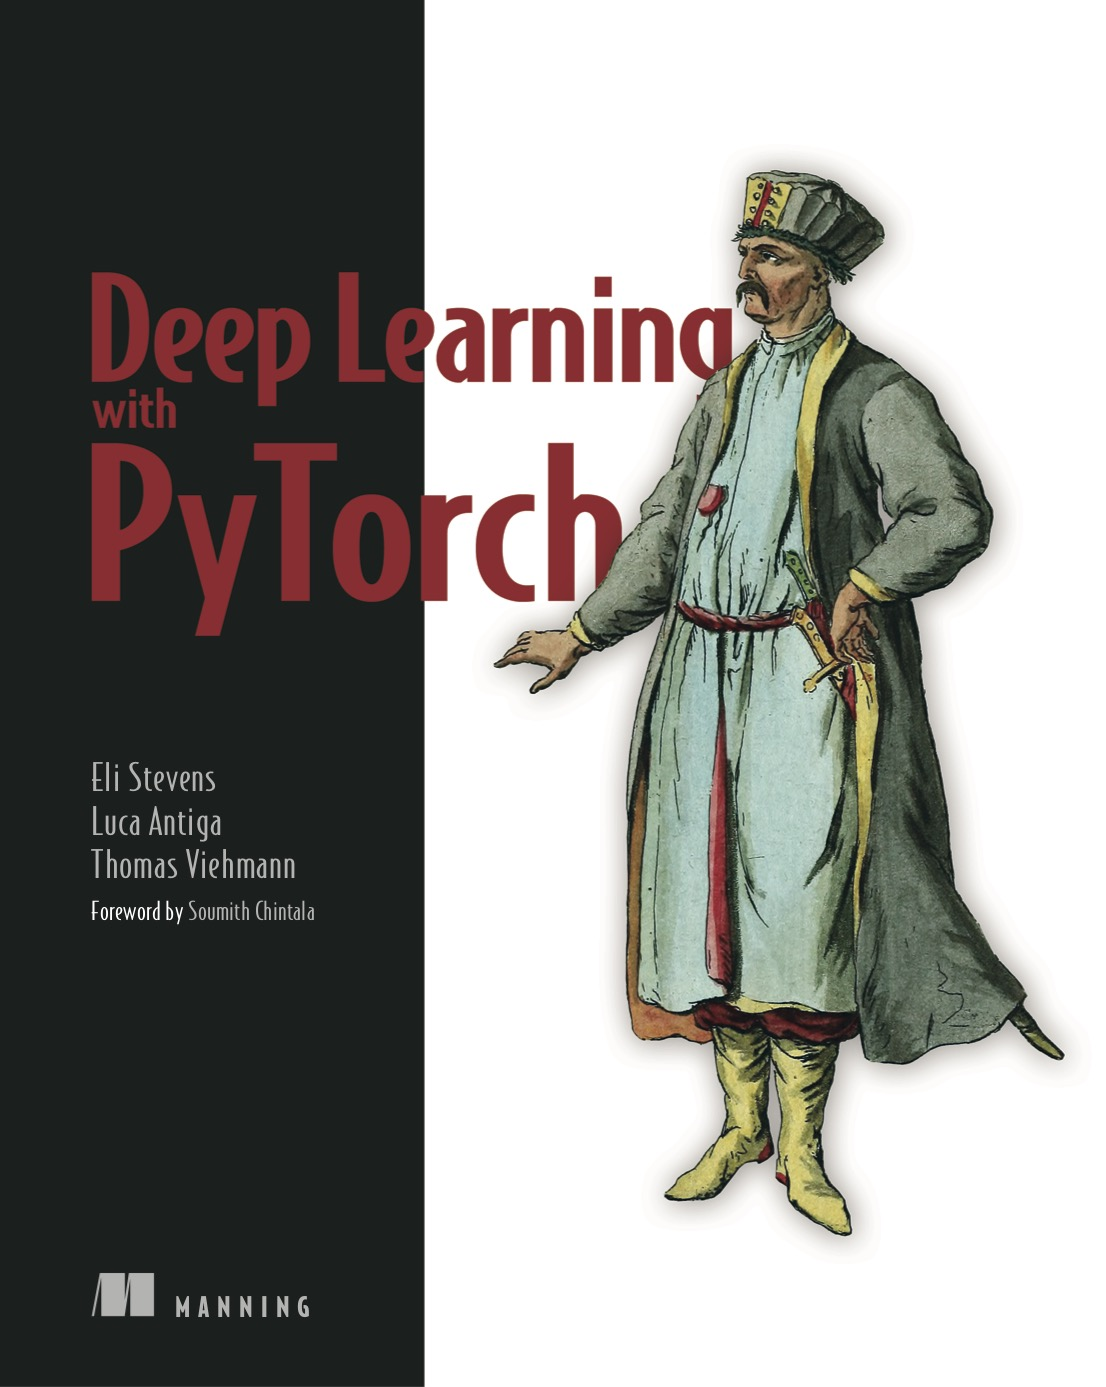
\includegraphics[width=0.45\textwidth]{deep-learning-thumbnail.png}
\end{figure}

48学时可以讲授到第七章

\subsection{NLP 2019相关顶会}
\href{https://github.com/zggl/NLP-Conferences-Code}{NLP 2019相关顶会}

\href{https://live.bilibili.com/21689802}{百度顶会论文复现营2020}
%%%%%--------------------------------------------------
\subsection{ICLR 2020}
International Conference on Learning Representation, 2020年4月26日在埃塞俄比亚的首都亚的斯亚贝巴开展。共收到了 2594 篇论文,接收了 687 篇,接收率为 26.5\%。

\href{https://openreview.net/forum?id=rJeB36NKvB}{How much position information do convolutional neural network encode?}
卷积神经网络是局部滤波器,它在有限的区域内通过调整卷积核参数来提取特征,这意味着卷积滤波器能输出对应某个特征的响应,但是以往的研究对于CNN是否同时也编码了位置信息没有给出证明。在这篇文章中,作者检验了这个假设,揭示了在CNN中编码的绝对位置信息的惊人程度。一组综合性的实验证明了这一假设的有效性,并揭示了在深层CNNs中,位置信息是从何而来,以及如何表达这些信息(\href{https://www.paperdigest.org/2019/12/iclr-2020-papers-with-code/}{ICLR2020开源代码的paper集合})。

工信安全: 2019年中国人工智能产业发展指数
\end{pre} 
\pagestyle{empty}
\tableofcontents
\cleardoublepage
\include{tex/overview}
\mainmatter	  % 对正文用阿拉伯数字作为页码
%======================================================================
% 正文内容
\pagestyle{fancy}
\setcounter{page}{0}
%# -*- coding: utf-8-unix -*-
%%==================================================
% !Mode:: "TeX:UTF-8"
% !TEX TS-program = XeLaTeX
% !TEX encoding = UTF-8 Unicode
%%%%%%%%%%%%%%%%%%%%%%%%%%%%%%%%%%%%
\chapter{人工智能概述}
%%%%%%%%%%%%%%%%%%%%%%%%%%%%%%%%%%%%
\begin{tcolorbox}[colback=white!50,colframe=orange!50,title=人工智能]
\begin{center}
   人工智能(AI)是研究、开发用于模拟、延伸和扩展人的智能的理论、方法、技术及应用系统的一门技术科学.\hfill
\end{center}
\end{tcolorbox}
%%%%%%%%%%%%%%%%%%%%%%%%%%%%%%%%%%%%
\begin{tcolorbox}[colback=white!50, colframe=orange!50, title=李飞飞]
\begin{center}
   人工智能和机器学习仍然是一个进入门槛较高的领域,需要专业的知识和资源,很少有公司可以自己承担.\hfill
\end{center}
\end{tcolorbox}
注: 美国斯坦福大学计算机科学系教授,女,1976年出生于北京, 2015年12月入选2015年“全球百大思想者”. 2018年3月,获“影响世界华人大奖”.
现为美国斯坦福大学红杉讲席教授,美国国家工程院院士, 类人人工智能研究院 (HAI) 院长。

法国国民议会议员、数学家赛德里克·维拉尼 (Cédric Villani) 在其2018年提交的报告《有意义的人工智能》(For A Meaningful Artificial Intelligence) 中指出, “人工智能的雄心在于理解并复制人类认知”.
%%%%%%%%%%%%%%%%%%%%%%%%%%%%%%%%%%%%%
%\begin{figure}[htbp]
%	\centering
%	\includegraphics[width=0.75\textwidth]{AI20191218123051.jpg}
%   \label{AI20191218123051}
%\end{figure}
%AI20191218122945.jpg
%AI20191218123051.jpg
%%%%%%%%%%%%%%%%%%%%%%%%%%%%%%%%%%%%
%\begin{itemize}
%\item AI的定义及其研究目标
%\item AI的产生与发展
%\item AI研究的基本内容
%\item AI研究的不同学派
%\item AI的主要研究和应用领域
%\item AI近期发展分析
%\item 我国智能科学技术教育体系
%\end{itemize}
%%%%%%%%%%%%%%%%%%%%%%%%%%%%%%%%%%%%%%%%%%
\begin{figure}[H]
\centering
\includegraphics[width=0.6\textwidth]{AI191218001.jpg}
\label{AI191218001}
\end{figure}
%%%%%%%%%%%%%%%%%%%%%%%%%%%%%%%%%%
\begin{tcolorbox}[colback=white!50, colframe=orange!50, title=无名氏]
\begin{center}
   传承是无法避免的,对机器也是可以这么要求的.
\end{center}
\end{tcolorbox}
%%%%%%%%%%%%%%%%%%%%%%%%%%%%%%%%%%%%
\section{AI的定义及其研究目标}
%%%%%%%%%%%%%%%%%%%%%%%%%%%%%%%%%%%%
\subsection{AI的定义及其研究目标}
\begin{itemize}
\item 目前还没有 形式化定义

\item 一般解释: 人工智能就是用人工的方法在机器(计算机)上实现的智能,或称机器智能.

\item 无形式化定义的理由在于人工智能的严格定义依赖于对\uwave{智能}的定义: 即要定义人工智能,首先应该定义智能,  但智能本身也还无严格定义.
\end{itemize}
\begin{mydef}{人工智能-宋士吉}{1}
人工智能是研究、开发用于模拟、延伸和扩展人的智能的理论、方法、技术及应用系统.
\end{mydef}
因此,先对人类的自然智能进行讨论. \uwave{研究思路就是用人工智能逼近自然智能}.
%%%%%%%%%%%%%%%%%%%%%%%%%%%%%%%%%%%%
\subsection{何谓智能(自然智能)}
\begin{itemize}
\item 自然智能:指人类和一些动物所具有的智力和行为能力.

\item 人类的自然智能(简称智能):指人类在认识客观世界中, 由思维过程和脑力活动所表现出的综合能力.

\item 人类大脑如何实现智能: 不是很清楚人类大脑的信息处理机制和运行机理. 简单来说, 一个人可能在识别图片的时候由于各种劳累和马虎, 在这个数据集的错误率高于机器.
但是只要你去和它谈任何一个图片它所理解的东西, 比如一个苹果, 你都会震惊于其信息之丰富, 不仅包含了真实苹果的各种感官, 还包含了关于苹果的各种文学影视, 从夏娃的苹果, 到白雪公主的苹果.
应该说, 人类理解的苹果更加接近概念网络里的一个节点, 和整个世界的所有其它概念相关联,  而非机器学习分类器里的 $n$个互相分离的高斯分布(机器需要辨识苹果、树、草地和人等).
       大脑的化学反应的变化可以改变行为; Charles Robert Darwin 说: 人和高等动物, 显然只有程度上的区别, 种类上别无二致. 神经科学认为的一个假设是: 认知能力的提高跟大脑随着进化越变越大有关系.
\item 实现智能的两大难题之一: 宇宙起源和人脑奥秘; 然而, 我们对人脑奥秘知之甚少.

\item 目前已知关于人脑的知识

      人脑结构: $10^{11}-10^{12}$量级的神经元, 分布并行;

      人脑功能: 记忆、思维、观察、分析 等.

      脑结构的三个不同层面: \uwave{区域层面、细胞结构层面和分子层面}.

      \ding{172} 大脑皮层位于大脑的外部, 有点像一张覆盖在大脑其他部分之上皱巴巴的大抹布.
      人类大脑和其他灵长类动物大脑在体积上的差异, 主要是皮层增大所致.
      大脑皮层是高度关联的, 在大脑的所有连接中, 75\%位于皮层之内, 仅有25\%是通往大脑其他部分和神经系统的输入输出连接.

      \ding{173}\textbf{新皮层}是大脑皮层中较晚进化出来的区域, 它负责感官知觉、发出运动指令、进行空间推理和有意识思维, 也是智人语言产生的地方.
      解剖学将新皮层分为四个脑叶:\uwave{额叶、顶叶、颞叶和枕叶}. 对包括人类在内的灵长类动物而言, 新皮层大得异乎寻常.
      刺猬的新皮层占大脑重量的16\%, 夜猴(一种小型猴子)占46\%, 黑猩猩占76\%. 人类新皮层所占的比例则更大.

      当动物觉察到安全信息时,杏仁核-内侧前额叶-海马环路的theta同步化活动降低,而高频gamma同步化活动增强. 在恐惧记忆消退期间,杏仁核中间神经元的6~12 Hz 振荡及高频gamma (70~120 Hz) 振荡强度增加,与恐惧提取相关的低频gamma (30~70 Hz) 活动强度则降低, 另外,杏仁核的高频gamma与mPFC的theta振荡发生跨频段耦合,并接受来自mPFC的抑制性theta输入. 随着消退的进行,mPFC的高频 gamma振荡增强,以调节恐惧记忆的消退. 以人类为对象的研究结果显示,恐惧记忆的习得与dACC(图中橙色区域)相关,而vmPFC更多地参与到恐惧消退中.。在消退期间,vmPFC(图中红色区域)内低频gamma(36~44 Hz) 活动减弱。与此同时,海马通过调控情景信息参与到恐惧记忆的消退中(图中绿色所示为人类研究结果,蓝色所示为动物研究结果)。

    \begin{figure}[H]
    \begin{center}
    \quad\quad\quad
    \includegraphics[width=0.45\textwidth]{Brocas2020012801.png}
    \includegraphics[width=0.416\textwidth]{Brocas2020012802.png}
    \end{center}
    \label{Brocas2020012801}
    \end{figure}
      Michael S. Gazzaniga认为新皮层枕叶包括初级视觉皮层, 也叫纹状皮层. 黑猩猩的纹状皮层占整个新皮层的5\%, 人类的纹状皮层只占2\%, 低于预期值.

      生物神经网络最基本的结构特点是多层, 无论是视觉, 听觉, 我们说基本的神经回路都有层级结构, 而且经常是六层. 这种纵深的层级, 对应的编码原理正是从具体特征到抽象特征的层级编码结构.
      最有名的莫过于祖母细胞, 这一思路直接催生了以 CNN 为代表的深度学习. 从图 \ref{Glutamine013001} 中的右侧子图可以看出,尼氏染色主要染的是细胞体,而高尔基染色主要染的是树突。
    \begin{figure}[H]
    \begin{center}\quad
    \includegraphics[width=0.44\textwidth]{15339cf86b99167476hd.jpg}
    \includegraphics[width=0.4\textwidth]{7ce83064897d1hd.PNG}
    \end{center}
    \caption{灵长类动物的初级视觉皮层分层结构,从左至右分别为黑猩猩,猕猴,松鼠猴,猫头鹰猴,狨猴,婴猴,狐猴,树鼩; 人脑的视觉皮层(尼氏染色);中:人脑的运动皮层(尼氏染色);右:半个月大婴儿的皮层(高尔基染色)}
    \label{Glutamine013001}
    \end{figure}

在进入学龄期这个时期后(7-12-18), 人的脑容量都能达到正常水平. 即使人与人之间在脑容量和褶皱结构有细微差异, 这种差异也不影响智力水平. 不过,这段时期脑内部各个功能区的灰质白质比例, 却的确开始发生很大变化.
总体来讲,这段时期人的脑灰质占比是不断缓慢下降的,而白质占比则不断增高.
    \begin{figure}[H]
    \begin{center}\quad
    \includegraphics[width=0.44\textwidth]{Nao20200204083453.jpg}
    \end{center}
    \caption{不同时期脑部神经细胞密度}
    \label{Glutamine013001}
    \end{figure}
%%%%%-----------------------------------------------
\paragraph{动物在做决定时如何利用环境}

2020年3月20日,南加州大学,复旦大学等全球296家单位协作在Science发表题为“The genetic architecture of the human cerebral cortex”的研究论文,该研究对来自51,665个人的脑磁共振成像数据进行了全基因组关联荟萃分析,研究人员分析了整个皮质和34个已知功能脑区域的表面积和平均厚度。

该研究确定了199个重要的基因座,并发现了显著富集的基因座,可影响产前皮质发育过程中活跃的调节元件内的总表面积,支持放射状单位假说。影响区域表面积的基因座聚集在Wnt信号通路中的基因附近,从而影响祖细胞的扩增和脑区域身份。皮层结构的变化与认知功能,帕金森氏病,失眠,抑郁,神经质和注意缺陷多动障碍在遗传上相关。总而言之,这项工作确定了与皮质表面积和皮质厚度相关的全基因组重要位点,并使人们对人类大脑皮层的遗传结构及其模式有了更深入的了解。
人的大脑皮层是大脑的外部灰质层,涉及更高的认知功能的多个方面。其独特的折叠模式具有凸(回旋)和凹(沟)区域的特征。计算脑图绘制方法使用跨单个皮层的一致折叠模式来标记脑区域。在胎儿发育过程中,兴奋性神经元(皮质中主要的神经元细胞类型)是由发育中的生发区的神经祖细胞产生的。皮质表面积(SA)的扩大是由这些神经祖细胞的增殖驱动的,而厚度(TH)由其神经原性分裂的数目决定。皮质SA和TH的整体和区域测量值的变化已可靠地与神经精神疾病和心理特征相关联。
\begin{figure}[H]
    \begin{center}\quad
    \includegraphics[width=0.44\textwidth]{Brain20200322112102.jpg}
    \end{center}
    \caption{识别遗传因素对人体皮质结构的影响}
    \label{Brain20200322112102}
\end{figure}


%%%%%-----------------------------------------------
\paragraph{动物在做决定时如何利用环境}
2020年3月发表在的《神经元》(\href{https://www.cell.com/neuron/fulltext/S0896-6273(20)30061-1}{cell: Neuron-Context-Dependent Decision Making in a Premotor Circuit})杂志上 的一项研究发现, 这种利用环境的能力与老鼠大脑中一个被称为前外侧运动皮层(ALM)的区域, 以前人们认为它主要指导和计划运动. \index{前外侧运动皮层}
这一发现为大脑非凡的决策能力提供了新的视角.
灵活的决策是理解周围环境的关键工具; 所处环境的使用允许决策者通过考虑上下文环境来对相同的信息做出不同的反应.
“环境相关的决策是人类高级认知功能的基石, ”神经学家Michael Shadlen博士说. “就像我们今天的研究一样, 在老鼠大脑的运动区域观察这个过程, 让我们更接近于了解脑细胞和神经回路层面的认知功能. ”

\begin{newexam}
  “如果有人在冷清的街道上不舒服地站在我身边, 我可能会试图逃跑, 但如果同样的事情发生在拥挤的地铁车厢里, 我就不会感到这样的危险, ”神经学家和第一作者郑(赫伯特)吴博士说. “我搬家或不搬家的决定取决于我所处的环境;从而为我所做的选择提供一个理由. ”
\end{newexam}

\begin{newexam}
研究小组调查了大脑中几个专门处理和整合感觉信息的区域, ALM关键区域是运动皮层的一部分.
先前的实验表明, ALM有一个相对简单的工作: 引导老鼠舌头和面部肌肉运动.
基于这一认识, 研究人员设计了一项新的实验, 要求老鼠利用舌头和嗅觉系统做出灵活的决定, 而嗅觉系统是嗅觉的向导. 在实验中, 一只老鼠第一次闻到一种气味.
老鼠必须记住这种气味, 因为在短暂的停顿之后, 研究人员将另一种气味喷到老鼠的鼻孔上. 如果两种气味相同, 老鼠必须舔左边的管子才能得到水. 如果两种气味不同, 它必须向右舔一根管子.
\end{newexam}

先前在这类“延迟匹配样本”测试中所做的工作, 会让人认为老鼠会利用大脑中专门负责嗅觉的区域来决定舔食的方式. 来自这些区域的大脑活动记录似乎证实了这一机制.
“根据这些记录, 我们可以想象, 当老鼠闻到第二种气味时, 这些大脑区域就有了答案, ”Shadlen博士说. “剩下要做的就是把这个答案传递给大脑的运动系统, 从而产生对左右舔的适当反应. ”
如果是这样, 那么运动区域就不应该起作用, 直到提供了第二种气味, 而老鼠决定这两种气味是相同的还是不同的. 吴博士想出了一个聪明的方法来验证这个预测. 他关掉了老鼠的ALM, 直到发出第二种气味, 然后及时打开ALM, 让老鼠得到答案.
按照标准的观点, 老鼠应该不会被这种操作所影响, 因为它们的嗅觉系统仍然完好无损. 相反, 他们在这项任务中受到了损害. ”Michael Shadlen, 医学博士, 研究论文的合著者, 哥伦比亚大学祖克曼研究所神经学家
吴博士说:“我们的研究结果表明, 我们需要ALM来解决两种气味是否匹配的问题, 然后再决定舔到哪里, 这促使我们重新思考大脑是如何做出这些决定的. ”
ALM与气味感知无关.

\begin{newexam}
吴博士仔细观察了ALM中的脑细胞. 他在离大脑表面很近的地方发现了一种新的神经元, 这种神经元对第一种气味有反应. 它将这些信息放在手边, 直到接收到第二种气味.
为了探索这一意想不到的结果, 研究小组求助于理论神经学家Ashok Litwin-Kumar博士, 以调查多种可能解释ALM作用的潜在机制.
“传统观点认为, 动物的嗅觉大脑区域应该自己处理气味, 然后将信息反馈给ALM, 后者将指导舌头, ”Litwin-Kumar博士说. “但数据告诉我们一个不同的故事;第一种气味作为一种上下文线索, 刺激ALM, 然后通过决定舔第二种气味的方式来表明这种关系. ”
\end{newexam}

今天的发现, 虽然集中在ALM上, 但对于如何让科学家对整个大脑功能有更大的理解是很重要的.
“最终, 我们想要阐明解释简单行为的基本原理, 但这也为深入了解人类的高级认知功能提供了思路, ”Shadlen博士说. 要实现这个目标, 关键的一步是用生物学和数学的语言把有关神经元、回路和行为的知识结合起来. 这个合作项目凸显了这一战略的前景. ”

%%%%%-----------------------------------------------
\paragraph{分布强化学习的AI研究}
DeepMind与哈佛大学的研究人员受最近关于分布强化学习的AI研究启发, 提出了一种基于多巴胺的强化学习的方法 \cite{DabneyKurth-Nelson2020-9599}.
和AI系统类似, 大脑不是以“平均值”的方式预期未来可能的回报, 而是以“概率分布”的方式来预期, 从而证明大脑中存在“分布强化学习”. 大脑进行强化学习, 类似于顶级AI算法
“大脑中的多巴胺是一种代表惊讶(surprise)的信号. ” Will Dabney说: “当情况好于预期时, 就会释放出更多的多巴胺. ”

生物神经系统包含种类丰富的抑制型神经元, 它们往往在生物神经网络起到调控功能, 如同控制信息流动的路由器, 在合适的时候开启或关闭某个信号.
当下的 AI 直接用 attention 的机制 (把注意力集中放在重要的点上, 而忽略其他不重要的因素. 重要程度的判断取决于应用场景和主题的认识感知程度. 根据应用场景的不同, Attention分为空间注意力和时间注意力, 前者用于图像处理, 后者用于自然语言处理), 或者 LSTM 里的输入门来调控是否让某个输入进入网络, 其它一点类似路由器的作用, 但是种类和形式的多样性远不及生物系统. 皮层内的神经元都采取簇状结构, 细胞之间不是独立的存在, 而是聚集成团簇, 犹如一个微型的柱状体. 这些柱状体成为信息传输的基本单元. 图\ref{Glutamine013001}的右侧子图是初级感觉皮层(左)和初级运动皮层(右)的分层结构, 可以看到初级感觉皮层的第四层最厚, 而初级运动皮层的第四层特别薄.
    \begin{figure}[H]
    \begin{center}\quad\quad\quad
    \includegraphics[width=0.355\textwidth]{Glutamine013001.PNG}
    \includegraphics[width=0.4\textwidth]{sjpc4792a5d1hd.jpg}
    \end{center}
    \caption{兴奋型和抑制型神经元; 皮质小柱}
    \label{Glutamine013001}
    \end{figure}

  意识可以理解为自我对自我本身的感知.  关于意识的起源, 已经成为一个重要的神经科学探索方向, 意识与多个脑区协同的集体放电相关(The controversial correlates of consiousness – Science 2018).  但是, 关于意识的一个重大疑团是它对认知和智能到底有什么作用, 还是一个进化的副产物.

  人类大脑海马区神经元放电峰值频率500Hz, 以此推断人类大脑最大计算频率为500hz, 而现在普通电脑的cpu运算也是3.0ghz 以上, 而且还是4核芯, 每秒理论运算次数达到了惊人的120亿次, 运算速度已经远远超过人类大脑. 机器学习认知方面 当下展示出来的智力水平最多也就是3-5岁的小孩子, 计算效率存在差异.
\item 对智能的严格定义有待于人脑奥秘的揭示, 进一步认识.
\end{itemize}
%%%%%%%%%%%%%%%%%%%%%%%%%%%%%%%%%%%%
\subsection{认识智能的几种理论}
\begin{itemize}
\item 思维理论

     智能来源于思维活动, 智能的核心是思维, 人的一切知识都是思维的产物. 可望通过对思维规律和思维方法的研究, 来揭示智能的本质.
\item 知识阈值理论

     智能取决于知识的数量及其可运用程度. 一个系统所具有的可运用知识越多, 其智能就会越高.
\item 进化理论

     是美国MIT的Brooks在对人造机器虫研究的基础上提出来的. 智能取决于\uwave{感知}和\uwave{行为}, 取决于对外界复杂环境的适应, 智能不需要知识、不需要表示、不需要推理, 智能可由逐步进化来实现.
\end{itemize}
%%%%%%%%%%%%%%%%%%%%%%%%%%%%%%%%%%%%
\subsection{智能的层次结构}
各种理论的观点不一致, 从层次结构来说
\begin{itemize}
\item 高层智能: 以大脑皮层(抑制中枢)为主, 主要完成记忆、思维等活动.
\item 中层智能: 以丘脑(感觉中枢)为主, 主要完成感知活动.
\item 低层智能: 以小脑、脊髓为主, 主要完成动作反应活动.

\end{itemize}
\begin{remark}
\textit{不同观点在层次结构中的对应关系}: \textbf{高层智能}: 思维理论、知识阈值理论、进化理论 . 对应基础层. \textbf{中层智能}和低层智能分别对应技术层和应用层.
\end{remark}
%%%%%------------------------------------------
\begin{think}
  大脑是深度学习吗? \index{深度学习}
\end{think}
\begin{remark}
大脑是一个复杂得难以想象的东西, 它把许许多多结构不同的东西包括在内, 而我们对大脑的了解还太少; 大脑是不是深度学习, 我们还给不出确定的答案. 大脑总体来说不是深度学习, 不过其中的某一些子模块可以用深度学习来描述, 或者是部分符合深度学习的, 比如视觉皮层就有深度层次化的特征表征, 即便这些表征不都是学习得到的;视觉皮层也是深度学习的研究中重要的灵感来源.
\end{remark}
%%%%%%%%%%%%%%%%%%%%%%%%%%%%%%%%%%%%
\subsection{智能包含的能力}
\begin{itemize}
\item 感知能力: 通过感知器官感知外界的能力. 是人类获得外界信息的基本途径, 其处理方式有以下两种:

     \qquad$\bullet$ 感知-动作方式: 对简单、紧急信息.

     \qquad$\bullet$ 感知-思维-动作方式: 对复杂信息.
\item 记忆能力

      \textbf{记忆}: 对感知到的外界信息和由思维产生的内部知识的存储过程.

\item 思维能力
         \textbf{思维}: 对已存储信息或知识的本质属性、内部知识的认识过程.

         思维方式:
         \begin{itemize}
           \item 抽象思维(逻辑思维): 根据逻辑规则对信息和知识进行处理的理性思维方式.
           \begin{example}
             逻辑推理等.
           \end{example}
           \item 形象思维(直感思维): 基于形象概念, 根据感性形象认识材料对客观现象进行处理的一种思维方式.
           \begin{example}
             图像、景物识别等.
           \end{example}
           \item 灵感思维(顿悟思维): 是一种显意识和潜意识相互作用的思维方式.
           \begin{example}
             因灵感而顿时开窍.
           \end{example}
         \end{itemize}

\item 学习和自适应能力
      \begin{itemize}
       \item 学习: 是一个具有特定目的的知识获取过程, 是人的一种本能. 不同人的学习方法、能力不同.
       \item 自适应: 是一种通过自我调节适应外界环境的过程, 是人的一种本能. 不同人的适应能力不同.
      \end{itemize}
\item 行为能力: 是人们对感知到的外界信息作出动作反应的能力.
     \begin{itemize}
       \item 信息来源: 由感知直接获得的外界信息,  经过思维加工后的信息.
       \item 实现过程: 通过脊髓来控制(来自四肢和躯干的各种感觉冲动都是通过脊髓的\uwave{上行纤维束来传导}, 即传导面部以外的痛觉、温度觉和粗触觉的脊髓丘脑束、传导本体感觉和精细触觉的薄束和楔束等,以及脊髓小脑束的小脑本体感觉). 由语言、表情和体姿等来实现.
    \end{itemize}
\end{itemize}
%%%%%%%%%%%%%%%%%%%%%%%%%%%%%%%%%%%%
\subsection{何谓人工智能?}
%%%%%%%%%%%%%%%%%%%%%%%%%%%%%%%%%%%%
\begin{tcolorbox}[colback=white!50, colframe=orange!50, title=UC Berkely人工智能系统中心创始人兼计算机科学专业教授Stuart Russell]
\begin{center}
   \textbf{人工智能}是研究\uwave{让计算机展现出智慧}的方法. 计算机获得正确方向后就可以高效工作, 这里的正确的方向意味着最有可能实现目标的方向(术语就是最大化效果预期).
   人工智能需要处理的任务包括\uwave{学习、推理、规划、感知、语言识别和机器人控制}等.\hfill
\end{center}
\end{tcolorbox}
%%%%%%%%%%%%%%%%%%%%%%%%%%%%%%%%%%%%

\textbf{标志事件}:AlphaGo基于人工智能的增强技术和深度学习技术,战胜了李世石. 该技术利用大量的数据来训练神经网络, 从而对新数据做出预测行为.

     谷歌旗下的多款其他产品, 如地图、照片和邮箱等产品都开始利用这种技术增强用户体验; 谷歌翻译也将引入这种技术.

     引入深度学习技术的机器翻译软件, 有望达到人工翻译的水准(AlphaGo的改良版AlphaGo Zero使用了新一代的阿法元, 完全从零开始, 不需要任何历史棋谱的指引, 更不需要参考人类任何的先验知识, 完全靠自己一个人强化学习和参悟, 棋艺增长远超阿法狗, 目前的战绩是百战百胜, 击溃阿法狗的记录是100:0).

     Google翻译尝试在部分功能上使用深度学习技术,
     \begin{example}
       利用摄像头即时取词翻译, 这相当于同声传译. 在国内, 微信、QQ等都能取词翻译.
     \end{example}
\begin{remark}
  人工智能是一门专业性很强的计算机科学, 随着各大技术公司和学界的不懈努力, 这项技术未来会惠泽大众, 会给生活带来实实在在的好处.
\end{remark}

\textbf{对人工智能的常见误解}
\begin{itemize}
\item 「人工智能是一个特定技术」. 例如在二十世纪八十年代到九十年代, 人们经常将人工智能与基于规则的专家系统混为一谈. 现在则是将人工智能经常会与多层卷积神经网络混淆. 这有点像把物理和蒸汽机的概念搞混了. \uwave{人工智能探究如何在机器中创造智能意识}, 不是研究中产生的任何特定技术.
\item 「人工智能是一个特定类别的技术方法」. 例如, 经常有人用符号化或逻辑化的方法将人工智能与「其他方法」相互比较, 如神经网络和遗传编程. 人工智能不是一种方法, 它是一个课题. 所有这些方法都是在对人工智能进行研究的产物.
\item 「人工智能是一小群研究者的方向」. 这个误解与前几个错误有关. 一些作者\uwave{使用「计算智能」来指代几个特定的研究者群体, 如研究神经网络, 模糊逻辑和遗传算法的研究者}. 这是非常片面的, 这种分类方式让人工智能的研究陷入孤立境地, 研究成果不能得到广泛的注意.
\item 「人工智能只是算法」. 严格说来不算是误解, 人工智能的确包含算法(也可粗略定义为程序), 它也包含计算机中其他的应用. 当然, 人工智能系统需要处理的任务相比传统算法任务(比如排序、算平方根)复杂得多.
\end{itemize}
综合各种不同观点, 仅从\textbf{能力}和\textbf{学科}两个方面讨论人工智能:
\begin{itemize}
\item 能力方面: 人工智能就是用人工的方法在机器(计算机)上实现的智能, 或称机器智能.
\item 学科方面: 是一门研究如何构造智能机器或智能系统, 以模拟、延伸和扩展人类智能的学科.
\item Turing测试: 如图\ref{AI:turingFig1}所示. 能分辨出人和机器的概率小于50\%.
\begin{remark}
  Turing测试存在的问题: 仅反映了结果的比较, 不涉及思维过程, 没指出是什么人.
\end{remark}
\end{itemize}

---Turing测试(图{AI:turingFig1})
\begin{figure}[htbp]
\begin{center}
\begin{tikzpicture}[font={\sf \small}]
\def \smbwd{2cm}
\def \smbwe{4cm}
\node (Gei) at (2,0) [draw, process,minimum width=\smbwd, minimum height=0.5cm] {图灵测试}; % 给
\node (ZCR1)[align=center,below=2cm of Gei,yshift=0cm] {\includegraphics[width=0.25\textwidth]{turing120191201.png}};
\node (TZCR1)[align=center,below=1.8cm of Gei,yshift=-4.5cm] {测试主持人};
\node (JQ1)[align=center,left=2cm of Gei,yshift=0cm] {\includegraphics[width=0.25\textwidth]{turing220191201.png}};
\node (TJQ1)[align=center,left=2.3cm of Gei,yshift=-1.85cm,xshift=0.25cm] {被测机器};
\node (BCR1)[align=center,right=2cm of Gei,yshift=0cm] {\includegraphics[width=0.25\textwidth]{turing320191201.png}};
\node (TBCR1)[align=center,right=2.3cm of Gei,yshift=-1.85cm] {被测人};
\draw[thick,blue,<->] (0,-5) parabola (-3,-1.5);
%加上bend at end 属性, 就会以终点为抛物线顶点.
\draw[thick,blue,<->] (4,-5) parabola (7,-1.5);
%%\draw[green] (-0.5,3) parabola bend (0,0) (2,3);%相当于画了两条顶点相同抛物线,
\end{tikzpicture}
\end{center}
\caption{图灵测试}
\label{AI:turingFig1}
\end{figure}
%%%%%%%%%%%%%%%%%%%%%%%%%%%%%%%%%%%%
\subsection{人工智能的近远期目标}
\begin{itemize}
\item 远期目标: 揭示人类智能的运行机理, 用智能机器去模拟、延伸和扩展人类的智能.
              涉及到\uwave{脑科学、认知科学、计算机科学、系统科学、控制论等多种学科的共同发展}.

\item 近期目标: 研究如何使现有的计算机更聪明, 即使它能够运用知识去处理问题, 能够模拟人类的智能行为.

\item 相互关系: 远期目标为近期目标指明了方向. 近期目标则为远期目标奠定了理论和技术基础.
\end{itemize}
%%%%%%%%%%%%%%%%%%%%%%%%%%%%%%%%%%%%
\subsection{人工智能对计算机科学的影响}
人工智能时代的来临, 给计算机体系结构的创新带来了新的黄金时代, 挑战的同时也要抓住机遇.

在过去的 50 年间, 人工智能的发展经历了三次起伏, 其中的三大关键因素便是\textbf{算法、大数据和算力}.
而在当下的第三次浪潮中, 软件和硬件的融合成为新的趋势, 其中 AI芯片更是成为了此次浪潮中极为重要的因素. 传统意义上的软件公司如 Facebook、亚马逊, 以及中国的互联网企业都开始涌入这一领域.
这一形势下, 呈现出百花齐放的形势, 让硬件研发存在更多的可能性.
具体而言, 可以探索的三个大方向:

一、\Circled{异构计算}. AI 时代没有哪一个单独的芯片能够做到一统天下, 如 CPU、GPU、FPGA 这些不同的通用芯片, 各有其优势, 未来可能需在同一个平台上使用不同的芯片. 研究异构计算方法, 提高高性能分布式系统的训练效率.

二、\Circled{专用 芯片}. 从谷歌在 2017 年发布的第一款 ASIC TCP——TPU, 到阿里前不久发布的平头哥含光 900芯片, 这些专用的芯片相比通用芯片的优势非常明显. 都是为特定的场景定制, 功耗低、成本低以及性能优.

三、\Circled{围绕存储做新架构探索}. AI 时代对存储的带宽容量的要求非常高, 计算过程中将数据从存储搬到计算单元、再从计算单元搬回存储中所需的容量和性能损失远远超过做计算本身. 因此, 当下 AI 硬件创新面临的一个很重要的挑战, 就是存储墙. 有两个探索方向:

方向 一是利用 3D 堆叠技术解决未来计算中的存储带宽问题. AMD 于 2015 年发布的 Fiji 核心便是这一思路的产物, 其可以直接用 Fiji GPU 来加速 DNN, 性能大幅提高. 现在, 几乎所有 AI 芯片公司都会沿用这一思路, 考虑在芯片训练中使用这种 HBM(高带宽存储器).

方向二是计算存储一体化, 这是未来有可能改变传统的把计算和存储分开的冯·诺依曼架构的一个方向, 并且这种方法不仅仅改变计算机体系结构, 还能在材料、底层半导体技术上做更新. 其中一个比较有趣的工作便是 ReRAM 技术, 能够让计算和存储发生在同一个地方, 而不需要做数据的搬移, 节省的能耗和提高的性能非常多.

AI 时代, 可以探索到计算机体系结构前沿主题, 从底层看, 可以尝试异构计算、3D 堆叠以及计算存储一体化等; 往上看, 则是在应用层做创新.

AI 计算系统体系提出了一致的愿景:未来的 AI 计算应该是分等级的分布式计算系统, 即从云到边缘设备再到终端设备, 让不同等级的数据在不同的地方进行计算和处理, 从「AI in Cloud」变成「AI Everywhere」.
而要实现这一愿景, 还面临着一个难题:计算需求和功耗受限之间的矛盾. 具体到 AI 芯片设计上, 则主要有以下三个主要的挑战:

1) 来自于可编程能力. 也就是说, 随着算法的演进, AI 芯片能够通过编程得到持续改进.

2) 来自于 AI 芯片落地应用处理任务时, 不仅需要处理神经网络, 还需要处理大量常规的计算或经典的信号处理计算.

3) 能耗问题, 尤其是对于边缘设备或者物联网设备而言, 能耗问题非常突出.

为了实现这种超高能效、可编程又具有灵活性的计算, 在过去六七年的时间里已经有了相当多的工作, 主要沿着两个方向努力:一个方向是算法方向, 对神经网络模型进行剪枝、压缩、量化、低位宽化; 另一个方向则是在领域专用的体系结构上的探索, 包括数据粒度、编程和存储模型等.

针对体系架构(尹首一教授等的一系列工作), 其中就包括采用基础的可重构计算架构来做 AI 计算芯片, 主要从 MAC 单元、PE 及 PE 阵列架构三个层面上实现了硬件的可重构能力. 采用这种架构设计出来的芯片, 不仅能够支持灵活的、不同神经网络的编程, 还能极大地降低能耗.
下一阶段, 尝试实现可重构、可编程的体系结构和存储计算一体化(In-Memory Computing)的融合. 「这样才是一个将来能够真正把计算和能效继续推高, 把芯片的适用性和灵活性继续扩大的 AI 芯片解决方案. 」

现在的计算逐渐从云端走向边缘端, 然而边缘端的计算目前还存在很多问题:一方面是移动设备「算不好」; 另一方面则是穿戴设备「算不了」. 而这些问题背后的原因主要还是边缘端的智能计算复杂度太高, 当前的芯片还无法满足这类边缘端计算的需求.
在过去很长一段时间, 国内学术界研究算法和研究硬件的人属于两个完全不同的领域, 各自「井水不犯河水」, 几乎很难一起做研究, 然而随着近几年来智能计算的发展, 尤其是深度学习模型对芯片架构提出了新的挑战和诉求, 计算和芯片二者在研究中结合得越来越紧密.

智能计算按应用领域分为\uwave{云端}和\uwave{边缘端}, 按任务可以分为\uwave{训练}和\uwave{推理}, 这四者可以组成四个象限:\uwave{云端训练、云端推理、边缘推理以及边缘训练}. 而随着目前智能计算走过了从云端训练到云端推理、再到边缘推理的阶段, 下一步可以探索边缘训练, 特别是随着 5G 通信的到来, 将为这一方向的探索带来了更多的机会(中国科学院自动化研究所南京人工智能芯片创新研究院常务副院长程健).

人工智能时代的到来使社会的生产要素发生了根本性变化. 生产力的三要素, 劳动者、劳动对象、劳动资料都在发生巨大变化, 这三要素都跟计算密切相关, 是人工智能计算是未来核心动力.

在农业时代、工业时代, 甚至信息时代, 劳动者没有发生太大的变化, 但是在智慧时代, 自然人和人工智能结合, 对劳动者的生产能力产生了极大的促进, 比如过去受自然环境的影响, 我们用人工去识别图像, 资料, 现在靠人工智能来做, 识别效率得到了成千上万倍的提升; 进入智慧时代, 数据成为重要的劳动对象, 以前的劳动对象, 是一种自然资源, 会在生产过程中, 消耗或转化, 而数据资源使用后仍然存在, 并且又生成了新的数据, 数据资源生生不息; 同时, 计算设备成为了新的劳动资料, 特别是人工智能时代, 劳动资料呈现指数级的需求.

“人工智能计算是未来核心动力, 代表着智慧计算的发展方向”(王恩东). 在人工智能计算中, 由于大场景、大计算需求越来越明显, 用通用芯片进行AI计算可能越来越不实用, 而更多的加速芯片会占据主流. 在这方面, 国内外很多的企业, 像谷歌、亚马逊、Facebook, 中国的BAT、浪潮, 都在AI领域不断的创新. 目前的AI计算服务, 一方面是以云的形式提供, 另一方面以物理服务器的形式提供.

目前, 浪潮在AI服务器领域, 中国市场占比超过50\%, 大部分AI企业使用浪潮服务器进行AI的深度学习和推理训练. 此外, 浪潮也在围绕AI算法优化、框架融合应用等方面持续创新.

人工智能推动了各个行业从信息化向智慧化升级, 提高了社会经济的效率, 并在多个行业引发了新一轮商业模式创新. 如在金融领域, 智能分析系统能够秒级完成人工一年36万小时的合同分析工作; 在制造领域, 一些大型的制造企业已经用智能机器人代替了50\%以上的劳动力. 从宏观来看, 人工智能发展将成为中国经济增长的新引擎, 相关数据显示, 到2035年人工智能领域的经济总量在整体经济的占比将达到20\%.
%%%%%%%%%%%%%%%%%%%%%%%%%%%%%%%%%%%%
\subsection{计算机科学与技术、软件工程、物联网、大数据专业的区别}
\begin{itemize}
\item 计算机科学与技术

计算机科学与技术专业是一个比较传统计算机类专业之一, 特点是注重基础知识结构的构建, 这个专业往往有较为全面的知识结构, 未来的就业面也相对更广一些, 目前很多IT行业的技术研发人员都是该专业毕业的.
不是该专业的人, 如果未来有明确的读研计划或者专业技能提升计划, 可以重点考虑一下计算机科学与技术专业, 未来在就业的方向上也会有更大的选择空间.

\item 软件工程

软件工程专业比较注重学生动手实践能力的培养, 相对于计算机科学与技术专业来说, 软件工程专业的知识结构也有所调整, 会增加一部分关于软件项目管理方面的课程, 更偏向于软件方面的知识.
软件工程专业近些年来的就业情况非常不错, 这与当前软件行业的快速发展有较为直接的关系.

\item 物联网

物联网专业的知识结构分为三大部分. 一、计算机硬件知识; 二、软件开发知识; 三、网络知识.
由于早期物联网领域的产业规模相对较小, 所以早期物联网专业的就业情况不太理想, 很多这个专业的人会选择软件开发领域的相关岗位.
但是, 随着5G的落地应用, 物联网未来的发展前景将非常广阔, 所以目前物联网专业也是热门专业之一.

\item 大数据

大数据专业是新开设的专业之一, 大数据专业在知识结构上与其他传统计算机专业的差别还是比较明显的, 重点增加了统计学相关知识, 同时还会增加一些行业领域的专业知识, 比如经济学、社会学、医学等, 不同高校会根据自身的实际情况来设置具体的课程体系.

\item 催生的新行业
智能制造工程技术人员、工业互联网工程技术人员、虚拟现实工程技术人员、人工智能训练师、连锁经营管理师、供应链管理师、网约配送员、电气电子产品环保检测员、全媒体运营师、健康照护师、呼吸治疗师、出生缺陷防控咨询师、康复辅助技术咨询师、无人机装调检修工、铁路综合维修工和装配式建筑施工员等16个新职业(2020年3月, 人力资源和社会保障部与市场监管总局、国家统计局联合向社会发布).
\end{itemize}
%%%%%%%%%%%%%%%%%%%%%%%%%%%%%%%%%%%%
\subsection{2020年十大科技趋势预测——百度研究院}
\begin{itemize}
\item 趋势1:AI技术已发展到可大规模生产的工业化阶段, 2020年将出现多家"AI工厂", 运用在各行各业帮助产业升级;
\item 趋势2:2020年将会是AI芯片大规模落地的关键年;
\item 趋势3:开源深度学习平台降低了技术开发门槛, 提高了AI应用的质量和效率, 深度学习技术将深入渗透到产业层面, 开始大规模应用;
\item 趋势4:自动机器学习AutoML将大大降低机器学习的门槛;
\item 趋势5: 多模态深度语义理解技术进一步成熟并将得到更广泛应用;
\item 趋势6:自然语言处理技术将与知识深度融合, 面向通用自然语言理解的计算平台得到广泛应用;
\item 趋势7:物联网将在边界、维度和场景三个方向形成突破 (突破云计算中心的边界, 向万物蔓延. 物理世界的时间和空间维度将被拓展. 物联网与能源、电力、工业、物流、医疗、智能城市等更多场景发生融合);
\item 趋势8:智能交通将加速在园区、城市等多样化场景中的落地;
\item 趋势9:区块链技术将以更加务实的姿态融入更多场景, 围绕区块链构建的数据确权、数据安全、数据使用、数据流通和交换等解决方案将在各行各业发挥巨大的作用;
\item 趋势10:量子计算将迎来新一轮爆发, 为AI和云计算注入新活力.
\end{itemize}

2019年3月召开的中央全面深化改革委员会第七次会议上, 审议通过了包括《关于促进人工智能和实体经济融合的指导意见》在内的八份文件, 是国家层面促进人工智能发展的又一份重要指导文件.
会议指出, \uwave{促进人工智能和实体经济深度融合, 要把握新一代人工智能发展的特点, 坚持以市场需求为导向, 以产业应用为目标, 深化改革创新, 优化制度环境, 激发企业创新活力和内生动力, 结合不同行业、不同区域特点, 探索创新成果应用转化的路径和方法, 构建数据驱动、人机协同、跨界融合、共创分享的智能经济形态}.

“\uwave{智能+}”被写入政府工作报告, 人工智能技术对社会的赋能被进一步提高. 在工业经济由数量和规模扩张向质量和效益提升转变的关键期, “智能+”的理念给人工智能等数字技术提供了最广阔的落地空间和回报想象. 通过智能化手段把传统工业生产的全链条要素打通, 可以更好地推动制造业的数字化、网络化和智能化转型, 更能反向助推技术自身的迭代和进步.

$\bullet$ 国产芯片和人工智能双突破

2019年8月, 清华天机AI芯片登上《自然》封面, 这也是中国芯片和人工智能领域第一次登上《自然》杂志. 作为全球首款异构融合类脑芯片, 它让自行车实现“无人驾驶”. 据报道, 天机芯片采用多核架构, 有多个高度可重构的功能性核, 可以同时支持机器学习算法和类脑电路. 从长远来看, 以通用人工智能为目标的“天机芯”, 如果真能实现自己的理想, 它将“无所不能”, 可用于各行各业.

$\bullet$ 人脸识别纠纷走上法庭

2019年9月初, 一款名为“ZAO”的APP火遍全网, 只需在APP中上传一张照片, 就能将自己的脸替换成大明星, 效果几乎以假乱真. 不过很快, 这款APP就因为涉嫌侵犯用户隐私受到争议, 用户上传脸部信息后, 将面临侵权、盗刷等安全风险. 另一边, 11月, 由于被强制要求刷脸入园, 浙江理工大学特聘副教授郭兵把杭州野生动物世界告上法庭, 这也成为国内人脸识别第一案.

$\bullet$ 新方法让机器人学习提速

2019年12月, 《自然》评出2019年度十大杰出论文, 其中包括苏黎世联邦理工学院用\textbf{数据驱动的方法设计机器人软件来训练四足机器人}, 大大提高了机器人的运动能力和学习速度. 新的训练方法利用强化学习, 使机器人学习的速度提升了1000倍, 动作灵活性和速度都大幅增强, 而且踢不倒, 甚至可以从跌倒中翻身站起. 四足机器人在实验室中的小跑速度已经提升了25\%, 在被推倒或滑倒后, 也能获得平衡, 重新站稳.

$\bullet$ 人脸识别国标开跑

人脸识别技术也在争议中探索着符合用户期待又不损害技术发展的治理模式. 在全国信标委生物特征识别分技术委员会换届大会上, 人脸识别技术国家标准工作组正式成立, 人脸识别国家标准制定工作全面启动.
随着人脸识别技术的广泛应用, 引发的问题也不可忽视, 如技术精度等性能标准缺乏导致的仿冒身份、用户授权被盗用等使用安全问题, 人脸信息收集、存储、处理等使用规范欠缺导致的信息泄露安全问题, 数据滥用、隐私保护缺乏规范等伦理问题. 公众也越发关注该技术在安全性上面临的挑战.

$\bullet$ 人工智能和宇宙

《生命3.0》让我们对人工智能和宇宙有了一个新的认识. 作者是美国迈克斯·泰格马克, 麻省理工学院物理系终身教授、未来生命研究所创始人.
%%%%%%%%%%%%%%%%%%%%%%%%%%%%%%%%%%%
\begin{example}
你说一束光有目标吗?
\end{example}
看起来没有, 向什么方向发射, 光就奔向哪个方向啊, 它自己能有啥目标?
但是, 你知道一个现象, 光线射入水中会发生折射. 光的路径不是一条直线, 而是一个折线.
为什么会这样呢?计算之后发现, 因为这样速度最快.
你可以想象一个救生员, 救生员在海滩上奔跑的速度快, 游泳的速度慢, 所以, 如果他要营救一个落水的游客, 最佳路线不是直直地过去, 而是在海滩上多跑一段, 在水里少游一段, 这样虽然看起来走了冤枉路, 但是总体花的时间最短.

同样道理, 光在空气中传播得快, 在水中传播得慢, 所以光会先在空气中多走一段, 再射到水中, 这样, 它到达目的地的速度更快.
你看, 奇怪吧. 光没有生命, 但是它居然会有自己的行动原则, 用最短时间从这一点到达那一点.
所以, 光的目标是什么?那就是在最短时间内到达目的地.
%%%%%%%%%%%%%%%%%%%%%%%%%%%%%%%%%%%%%%%%%%
\begin{figure}[H]
\centering
\includegraphics[width=0.46\textwidth]{AI30633d4.pdf}
\caption{生命3.0}
\label{AI30633d4}
\end{figure}
%%%%%%%%%%%%%%%%%%%%%%%%%%%%%%%%%%%%%%%%%%
\begin{figure}[H]
\centering
\includegraphics[width=0.76\textwidth]{AIUniverse0102.pdf}
\caption{营救溺水者的最佳路径和光的折射}
\label{AIUniverse0102}
\end{figure}
%%%%%%%%%%%%%%%%%%%%%%%%%%%%%%%%%%%
\begin{example}
那整个宇宙有没有这样的目标呢?
\end{example}
热力学第二定律说\index{热力学第二定律}, 就是追求“熵”的最大化. 简单说就是整个宇宙越来越无序、越来越混乱. 最后整个宇宙归于“热寂”.
\begin{remark}
就是万事万物都扩散成一种无聊而又完美的均质状态.
所有的星星都会熄灭, 所有的秩序都会变成混乱, 所有的地方温度都一样, 再也没有什么值得流动的了, 整个宇宙寂静了.
所以, 可以说宇宙的“目标”, 就是达到热寂.
\end{remark}
%%%%%%%%%%%%%%%%%%%%%%%%%%%%%%%%%%%
\begin{example}
超级人工智能时代, 人类来提供目标.

比如, 我们人类说, 地球太小了, 我们要更大的生存空间, 好, 人工智能就会造一个以恒星为动力源的戴森球.
比如, 人类说, 我想探索真理, 我们想把圆周率尽可能地算下去, 看看它到底有没有尽头, 人工智能就干脆熄灭一个星系的能量, 给人类算圆周率.
人类说, 我要星际旅行, 人工智能就帮你完成这个目标, 过程中耗掉无穷无尽的能量.
这也是一个合作, 人类提供意义和目标, 人工智能提供能力和方法. 这一合作, 宇宙走向热寂的大目标就能越来越快地达成.
\end{example}

\begin{center}
  “\uwave{发展中的问题, 发展中解决}”.
\end{center}
\begin{remark}
  人工智能的终极目标: 机器$\equiv$人.
\end{remark}
%%%%%%%%%%%%%%%%%%%%%%%%%%%%%%%%%%%%
\subsection{美国人工智能计划:2020年度报告}
2020年2月26日, 美国白宫科技政策办公室发布《“美国人工智能计划”:首个年度报告》(下称《报告》). 《报告》由美政府首席技术官克瑞西奥斯与副首席技术官帕克联合签发, 主要从投资AI研发、共享AI资源、消除AI创新障碍等方面, 总结了美政府过去一年在实施“美国人工智能计划”方面取得的重大进展.

《报告》指出, 美政府拥有大量数据、模型及计算资源等重要AI资源. 美政府努力使各界获得高质量、可追溯的AI资源, 支持AI研发, 主要举措包括:①2019年12月, 美政府发布《联邦数据战略2020年行动计划》, 指导各机构开发工具、完善流程, 高效使用数据. ②美国国家科学基金会与DARPA合作开展“实时机器学习”项目, 探索可在连续数据流中学习的硬件与机器学习架构;与联邦公路管理局合作研究隐私技术, 寻求远程访问高速公路数据库;资助加利福尼亚大学及华盛顿大学开发并运营“云银行”(CloudBank), 为计算机科学人员提供公共云. ③美国能源部为国家癌症研究所提供超级计算机, 开发治疗癌症的AI解决方案. 三、消除AI创新障碍《报告》认为, AI仍然处于起步阶段. 美政府发布多项文件以指导制定相关法律、法规及标准, 消除AI创新障碍, 快速推进AI发展, 包括:

\ding{172} 2019年4月, 美国食品药品监督管理局提出针对医疗AI软件的监管框架, 确保这些软件安全有效.

\ding{173} 2019年8月, 美国国家标准技术研究院发布《联邦政府参与开发技术标准与相关工具的计划》, 强调美政府应持续参与AI标准开发活动, 推进可信任AI技术发展.

\ding{174} 2020年1月, 美国运输部发布《确保美国在自动驾驶汽车技术中的领导地位:自动驾驶汽车4.0》文件, 详细阐述了美政府在自动驾驶汽车领域的若干原则. ④2020年1月, 美政府发布监管AI的10项原则, 包括公众信任、公众参与、科学诚信与信息质量等.
%%%%%%%%%%%%%%%%%%%%%%%%%%%%%%%%%%%%
%\subsection{José Luis García Vigil-未来十年预测12/26/2019: Report to Enrique Portillo}
%
%We went to the future ... and we came back to tell you the 5 technologies that will explode in the next decade
%
%Telepresence and brains 'connected to the cloud'. By 2030,  technology will take a leap that can go beyond our imagination.
%Flying cars. Talking robots. Interstellar travel Science fiction has raised scenarios that seemed crazy for decades,  but now are real possibilities thanks to the leaps and bounds of technology.
%Maybe we still don't see cars in the skies,  but there are already several companies with projects in development of flying taxis. Will people ever get to other planetary systems? We do not know,  but there are objects made by humans (the Voyager 1 and Voyager 2 probes,  launched in 1977) that are already in interstellar space,  billions of kilometers from our Sun. And from robots… well,  we should Ask Alexa,  Siri,  Cortana,  Google and even Sophia to see what they think.

%Beyond these achievements,  the power of technology has also extended to more everyday issues: the ‘plague’ of smartphones,  the era of internet connectivity and even electric cars.
%What will we expect by 2030? Experts in the sector tell us about the technologies that will be a trend in the next ten years and that will become as common as a cell phone in hand.
%Fuimos al futuro… y volvimos para decirte las 5 tecnologías que explotarán en la siguiente década
%El Financiero 26/12/2019: Reportaje a Enrique Portillo
%Telepresencia y cerebros 'conectados a la nube'. Hacia 2030,  la tecnología dará un salto que puede ir más allá de nuestra imaginación.
%Autos voladores. Robots parlantes. Viajes interestelares. La ciencia ficción ha planteado escenarios que hace décadas parecían una locura,  pero que ahora resultan posibilidades reales gracias al avance agigantado de la tecnología.
%
%Quizá todavía no vemos coches por los cielos,  pero ya hay diversas compañías con proyectos en desarrollo de taxis voladores. ¿Alguna vez las personas lograrán llegar a otros sistemas planetarios? No lo sabemos,  pero hay objetos hechos por humanos (las sondas Voyager 1 y Voyager 2,  lanzadas en 1977) que ya se encuentran en el espacio interestelar,  a miles de millones de kilómetros de nuestro Sol. Y de los robots… pues habríamos que preguntarle a Alexa,  Siri,  Cortana,  Google y hasta a Sophia a ver qué ‘piensan’.
%Más allá de estos logros,  el poder de la tecnología también se ha extendido a cuestiones más cotidianas: la ‘plaga’ de los smartphones,  la era de la conectividad a internet y hasta los autos eléctricos.
%¿Qué nos deparará hacia 2030? Expertos en el sector nos hablan de las tecnologías que serán tendencia en los siguientes diez años y que se volverán tan comunes como un celular en la mano.
%https://elfinanciero.com.mx/tech/fuimos-al-futuro-y-volvimos-para-decirte-las-5-tecnologias-que-explotaran-en-la-siguiente-decada
%%%%%%%%%%%%%%%%%%%%%%%%%%%%%%%%%%%%
\section{AI的产生与发展}

50多年来, 人工智能走过了一条起伏和曲折的发展道路. 回顾历史, 可以按照不同时期的主要特征, 将其产生与发展过程分为6个阶段.
\begin{itemize}
\item 孕育期(1956年以前);
\item 形成期(1956——1970年);
\item 知识应用期(1970——20世纪80年代末);
\item 从学派分离走向综合(20世纪80年代末到本世纪初);
\item 智能科学技术学科的兴起(21世纪初以来);
\item 深度学习为代表的人工智能技术(2010年以来).
\end{itemize}
%%%%%%%%%%%%%%%%%%%%%%%%%%%%%%%%%%%%
\subsection{AI的产生与发展-孕育期(1956年以前)}
%%%%%%%%%%%%%%%%%%%%%%%%%%%%%%%%%%%%
\paragraph{AI的产生与发展-孕育期(远古——1946年以前)}

自远古以来, 人类就有用机器代替人们进行劳动的构想: 公元前900多年我国有歌舞机器人流传的记载; 公元前850年古希腊有制造机器人帮助人们劳动的神话传说; 三国时的木牛流马.
\begin{itemize}
\item  亚里斯多德(Aristotle, 公元前384——公元前322): 古希腊伟大的哲学家和思想家, 创立了演绎法. 他提出的三段论至今仍然是演绎推理的最基本出发点.
\item  莱布尼茨(G. W. Leibnitz, 1646——1716): 德国数学家和哲学家, 把形式逻辑符号化, 奠定了数理逻辑的基础.
\item  图灵(A. M. Turing, 1912——1954): 英国数学家, 1936年创立了自动机理论, 自动机理论亦称图灵机, 是一个理论计算机模型.
\item  莫克利(J. W. Mauchly, 1907——1980): 美国数学家、电子数字计算机的先驱, 与他的研究生埃克特(J. P. Eckert)合作, 1946年研制成功了世界上第一台通用电子计算机ENIAC.
\end{itemize}
%%%%%%%%%%%%%%%%%%%%%%%%%%%%%%%%%%%%
\paragraph{AI的产生与发展-孕育期(1956年以前)}
\begin{itemize}
\item  麦克洛奇(W. McCulloch)和皮兹(W. Pitts): 美国神经生理学家, 于1943年建成了第一个神经网络模型(MP模型).
\item  维纳(N. Wiener, 1874—1956): 美国著名数学家、控制论创始人. 1948年创立了控制论, 使得控制论向人工智能的渗透, 形成了行为主义学派. 1954年, 钱学森在McGraw-Hill出版了《工程控制论》.
\item  图灵又于1950年, 发表题为《计算机能思维吗?》的著名论文, 明确提出了“机器能思维”的观点.
\end{itemize}
\begin{remark}
在人工智能诞生之前, 一些著名科学家就已经创立了数理逻辑、神经网络模型和控制论, 并发明了通用电子数字计算机. 为人工智能的诞生准备了必要的思想、理论和物质技术条件.
\end{remark}
%%%%%%%%%%%%%%%%%%%%%%%%%%%%%%%%%%%%
\subsection{AI的产生与发展-形成期(1956--1970年)}
AI诞生于一次历史性的聚会.
\begin{itemize}
\item  时间: 1956年夏季;
\item  地点: 达特莫斯 (Dartmouth)大学;
\item  目的: 为使计算机变得更“聪明” , 或者说使计算机具有智能.

\item  发起人:
      \begin{itemize}
          \item  麦卡锡(J. McCarthy) , Dartmouth的年轻数学家、计算机专家, 后为MIT教授.
          \item  明斯基(M. L. Minsky), 哈佛大学数学家、神经学家, 后为MIT教授.
          \item  洛切斯特(N. Lochester),  IBM公司信息中心负责人.
          \item  香农(C. E. Shannon), 贝尔实验室信息部数学研究员.
      \end{itemize}
\item  参加人:
      \begin{itemize}
          \item  莫尔(T. More)、塞缪尔(A. L. Samuel),  IBM公司.
          \item 塞尔夫里奇(O. Selfridge)、索罗蒙夫(R. Solomonff), MIT.
          \item 纽厄尔(A. Newell), 兰德(RAND)公司.
          \item 西蒙(H. A. Simon), 卡内基(Carnagie)工科大学.
      \end{itemize}
\item  会议结果:

     由麦卡锡提议正式采用了“Artificial Intelligence”这一术语. AI以“推理、 知识” 为重点.
\end{itemize}

\begin{itemize}
\item  心理学小组
    \begin{itemize}
        \item  1957年, 纽厄尔、肖(J.Shaw)和西蒙等人的心理学小组研制了一个称为逻辑理论机(Logic Theory Machine, 简称LT)的数学定理证明程序.
        \item  1960年研制了通用问题求解(General Problem Solving)程序. 该程序当时可以解决11种不同类型的问题, 如不定积分、三角函数、代数方程、猴子摘香蕉、河内梵塔、人—羊过河等.
    \end{itemize}
\item  IBM工程小组

     1956年, 塞缪尔在IBM704计算机上研制成功了具有自学习、自组织和自适应能力的西洋跳棋程序. 这个程序可以从棋谱中学习, 也可以在下棋过程中积累经验、提高棋艺. 通过不断学习, 该程序1959年击败了塞缪尔本人, 1962年又击败了一个州的冠军.
\item  MIT小组
    \begin{itemize}
       \item  1958年, 麦卡锡建立了行动规划咨询系统.
       \item  1960年, 麦卡锡又研制了人工智能语言LISP.
       \item  1961年, 明斯基发表了“走向人工智能的步骤”的论文, 推动了人工智能的发展.
    \end{itemize}
\end{itemize}

其他方面

     \ding{172} 1965年, 鲁宾逊(J. A. Robinson)提出了归结(消解)原理.

     \ding{173} 1965年, 费根鲍姆(E. A. Feigenbaum) 开始研究化学专家系统DENDRAL.
%%%%%%%%%%%%%%%%%%%%%%%%%%%%%%%%%%%%
\subsection{AI的产生与发展-知识应用期(1971--80年代末)}
%%%%%%%%%%%%%%%%%%%%%%%%%%%%%%%%%%%%
\subparagraph{失败的预言}

60年代初, 西蒙预言: 10年内计算机将成为世界冠军、将证明一个未发现的数学定理、将能谱写出具有优秀作曲家水平的乐曲、大多数心理学理论将在计算机上形成并被验证.
%%%%%%%%%%%%%%%%%%%%%%%%%%%%%%%%%%%%
\subparagraph{挫折和教训}
\begin{itemize}
\item  在博弈方面, 塞缪尔的下棋程序在与世界冠军对弈时, 5局败了4局.
\item  在定理证明方面, 发现鲁宾逊归结法的能力有限. 当用归结原理证明两个连续函数之和还是连续函数时, 推了10万步也没证出结果.
\item  在问题求解方面, 对于不良结构, 会产生组合爆炸问题.
\item  在机器翻译方面, 发现并不那么简单, 甚至会闹出笑话. 例如, 把“心有余而力不足”的英语句子翻译成俄语, 再 翻译回来时竟变成了“酒是好的, 肉变质了”.
\item  在神经生理学方面, 研究发现人脑有$10^{11-12}$以上的神经元, 在现有技术条件下用机器从结构上模拟人脑是根本不可能的.
\item  在其它方面, 人工智能也遇到了不少问题. 在英国, 剑桥大学的詹姆教授指责“人工智能研究不是骗局, 也是庸人自扰”. 从此, 形势急转直下, 在全世界范围内人工智能研究陷入困境、落入低谷.
\end{itemize}
%%%%%%%%%%%%%%%%%%%%%%%%%%%%%%%%%%%%

以知识为中心的研究:
\begin{itemize}
\item  专家系统实现了人工智能从理论研究走向实际应用, 从一般思维规律探讨走向专门知识运用的重大突破, 是AI发展史上的一次重要转折.

2020年3月, 日本诺日士钢机集团旗下的Doctor-NET(东京港区)将启动人工智能检测新型冠状病毒的实证试验. 该公司将与中国的AI开发企业北京推想科技合作, 向日本引进在武汉等地使用的新冠肺炎诊断系统.

\item  1972年, 费根鲍姆开始研究MYCIN专家系统, 并于1976年研制成功. 从应用角度看, 它能协助内科医生诊断细菌感染疾病, 并提供最佳处方. 从技术角度看, 他解决了知识表示、不精确推理、搜索策略、人机联系、知识获取及专家系统基本结构等一系列重大技术问题.
\item  1976年, 斯坦福大学的杜达(R. D. Duda)等人开始研制地质勘探专家系统PROSPECTOR.
\end{itemize}

这一时期, 与专家系统同时发展的重要领域还有计算机视觉和机器人, 自然语言理解与机器翻译等. 但直到80年代末,  所有的AI程序都只是“玩具”.

\textbf{新的问题}: 专家系统本身所存在的应用领域狭窄、缺乏常识性知识、知识获取困难、推理方法单一、没有分布式功能、不能访问现存数据库等问题被逐渐暴露出来.
%%%%%%%%%%%%%%%%%%%%%%%%%%%%%%%%%%%%
\subsection{AI的发展-知识深化期(1990-2000年代末)}
以“特征” 为重点

     \ding{172} 1993年, 支持向量机出现.  国内的王国俊教授提出了三I方法.  由于模糊推理与模糊逻辑在模糊控制中有直接的应用, 模糊推理与模糊逻辑的研究受到模糊系统与人工智能学界的广泛关注. 1997年3月在美国召开的国际信息科学联合会议上, 王国俊作了“\uwave{论模糊推理的逻辑基础}”的报告. 这一报告引起了很多与会代表的浓厚兴趣, 并受到前任国际模糊系统协会主席、纽约宾汉顿大学的Klir 教授以及 Turksen等著名教授在内的许多学者高度评价, 克雷顿大学模糊系统研究所所长Mordeson教授还在该校的研究报告中刊登王的全文. 如今这一成果已全文发表于Information Sciences.
       在此基础上, 王提出了模糊推理的三I方法, 于1999年发表于《中国科学》, 全面改进了传统的CRI方法. 2004年7月, 他在美国盐湖城召开的信息科学联合会议上当选为不确定性数学学会副理事长.

     \ding{173} 1992年, 美国控制论专家L. A. Zadeh教授指出:人工神经网络、模糊逻辑、遗传算法、蚁群算法与传统计算模式的区别, 在于它们与人脑对应, 具有在不确定及不精确环境中进行推理和学习的智能计算能力. 除此之外, 粗糙集方法、机器学习方法以及各种随机搜索技术等也被纳入到人工智能的统一框架中, 人工智能技术已在众多应用领域取得了极大的成功.

     \ding{174} 全蕴涵模糊推理机制与模糊规则的启发式生成方法.  模糊控制系统的核心技术是模糊控制器的设计,  模糊控制器的主要组成部分是\uwave{模糊推理机和模糊规则库}. 70 年代 L.A.Zadeh 教授提出的“复合蕴涵规则”方法虽得以广泛应用, 但模糊推理的基本形式FMP问题的合成推理方法求解使用的合成运算缺乏严格的逻辑依据, 模糊推理逻辑基础问题一直受到了科学家和工程师的极大关注, 同时也已取得了一系列有价值的研究成果. 其中以我国前辈数学家王国俊教授提出的“\uwave{全蕴涵模糊推理机制与推理方法}”受到了最为广泛的关注. 该推理方法在模糊推理的每一步运算过程都使用了蕴涵运算, 通过蕴涵算子给出模糊推理最优解的解析形式. 基于不同的蕴涵方式, 有学者提出了反向模糊推理机制与模糊推理算法, 给出了模糊取式和模糊拒取式最优解的解析计算公式.

     \ding{175} 模糊知识约简/模糊决策树生成模糊规则的启发式方法.  1982年Z. Pawlak教授提出的粗糙集理论在处理不完整、不一致和不精确数据的问题中取得成功, 目前已经发展成为一种较为成熟的定量分析数学工具, 在机器学习、数据挖掘、模式识别、故障诊断等领域有着广泛的应用. 其主要思想是将模糊相似关系代替粗糙集的等价关系, 引入模糊上、下近似概念, 并提出模糊约简与模糊核的定义, 提出了一种启发式算法能够从初始模糊数据中学习模糊规则, 该算法从真正意义上实现了从模糊数据抽取模糊规则. 项目进一步开展了模糊决策树归纳学习研究, 提出了一种产生模糊决策树的启发式算法, 将粗集核学习与决策树归纳进行结合, 可生成高性能加权模糊规则.

     \ding{176} 基于极限学习机或随机机会约束模型的智能学习方法.  极限学习机方法的前期工作仅适用于解决有监督的机器学习问题, 不能处理标签数据存在缺失的情形. 针对数据标签有缺失且带有分布流形特性的数据, 基于Laplacian矩阵的流形正则化思想学习数据的流形特性, 构造了两步骤学习的统一框架,  将有监督、无监督和半监督极限学习算法纳入其中. 进而项目研究了基于机会约束模型的有监督学习方法与半监督学习方法. 首先建立了基于随机机会约束的鲁棒支持向量非线性回归模型, 将随机约束优化问题转化为二次锥规划问题, 由内点法可实现高效求解, 解决了回归分析中输入数据和输出数据同时受到噪声干扰的问题.
%%%%%%%%%%%%%%%%%%%%%%%%%%%%%%%%%%%%
\subsection{数据智能——发展期(2000-2009年末)}

2006年, Geoffery Hinton提出深度学习, 使得神经网络得以重生.  关于人工智能的每一个进步都是由30年前的一篇阐述多层神经网络的训练方法的论文(Learning representations by back-propagating errors, \cite{RumelhartHinton1986-9415})演变而来, 它为人工智能在最近十年的发展奠定了基础, 但要保持这种进步, 就要面对人工智能严重的局限性.

多伦多市中心一栋高级大厦, 七层是新成立的人工智能研究所Vector Institute的所在地. 研究所的联合创始人乔丹·雅各布(Jordan Jacobs). 该研究所于今年秋天正式成立, 致力于成为全球人工智能中心.  为了拜访杰弗里·辛顿(Geoffrey Hinton)来到多伦多. 他是“深度学习”之父, 正是这个技术让人工智能发展到今天这般炙手可热. 雅各布说:“我们30年后再往回看, 杰弗里就是人工智能(我们认为深度学习就是人工智能)的爱因斯坦. ” 在人工智能领域最顶尖的研究人员当中, 辛顿的引用率最高, 超过了排在他后面三位研究人员的总和. 他的学生和博士后领导着苹果、Facebook和OpenAI的人工智能实验室; 辛顿本人是谷歌大脑(Google Brain)人工智能团队的首席科学家.

事实上, 人工智能在最近十年里取得的几乎每一个成就, 包括语音识别、图像识别, 以及博弈, 在某种程度上都能追溯到辛顿的工作.
Vector Institute研究中心进一步升华了辛顿的研究. 在这里, 谷歌、Uber、Nvidia等美国和加拿大的公司正努力将人工智能的技术商业化. 资金到位的速度比雅各布想象的更快; 他的两个联合创始人调研了多伦多的公司, 发现他们对人工智能专家的需求是加拿大每年培养的人数的10倍.
某种意义上, Vector研究所是全球深度学习运动的原爆点:无数公司靠这项技术牟利, 训练它、改进它、应用它. 到处都在建造数据中心, 创业公司挤满了摩天大楼, 整整新一代学生也纷纷投身这一领域.
%%%%%%%%%%%%%%%%%%%%%%%%%%%%%%%%%%%%
\subsection{数据智能——爆发期(2010-现在)}
\begin{figure}[H]
\centering
\includegraphics[width=0.86\textwidth]{AIhistory013001.PNG}
\caption{神经网络的发展\href{https://aistudio.baidu.com/}{历史}}
\label{AIhistory01300}
\end{figure}
%%%%%%%%%%%%%%%%%%%%%%%%%%%%%%%%%%
$\blacklozenge$ 2012年, 深卷积神经网络错误率下降到了16\%;在接下来的几年中, 错误率下降了几个百分点. 虽然2012年的突破是“前所未有的组合”, 但大幅量化的改进标志着全行业人工智能繁荣的开始. 到2015年, 研究人员报告说, 软件在狭窄的ILSVRC任务中超出人类能力. 然而, 作为挑战组织者之一的Olga\, Russakovsky在2015年指出, 这些计划只需将图像识别为属于千分之一的图像;人类可以识别更多的类别, 并且(不像程序)可以判断图像的上下文.
\begin{remark}
ILSVRC (ImageNet Large Scale Visual Recognition Challenge)是近年来机器视觉领域最受追捧也是最具权威的学术竞赛之一, 代表了图像领域的最高水平.

ImageNet数据集是ILSVRC竞赛使用的是数据集, 由斯坦福大学李飞飞教授主导\index{李飞飞}, 包含了超过1400万张全尺寸的有标记图片. ILSVRC比赛会每年从ImageNet数据集中抽出部分样本, 以2012年为例, 比赛的训练集包含128\,1167张图片, 验证集包含5E4张图片, 测试集为1E5张图片.

\end{remark}
$\blacklozenge$ 2014年, 超过50家机构参加了ILSVRC. 2015年, 百度科学家因使用不同帐户而被禁止使用一年, 大大超过每周两次提交的指定限制. 百度后来表示, 它解雇了涉及的团队领导, 并建立了一个科学咨询小组.

$\blacklozenge$ 2016年, AlphaGo在一场复杂的围棋比赛中打败了世界冠军, 震惊了计算机科学家们. 它背后的DeepMind团队中的重要成员曾是特南鲍姆的博士后. 特南鲍姆参与了一家创业公司的工作, 这家公司致力于让自动驾驶汽车直观地了解一些基础物理学, 对其他驾驶员的意图也能做出一定的直觉判断, 从而更好地应对从未遇到过的情况, 比如一辆卡车冲到前面或他人强行超车.

$\blacklozenge$ 2016年,  以“学习” 为重点, 出现了\href{http://www.image-net.org/}{ImageNet数据库}. ImageNet项目是一个用于视觉对象识别软件研究的大型可视化数据库. 超过1400万的图像URL被ImageNet手动注释, 以指示图片中的对象;在至少一百万个图像中, 还提供了边界框. ImageNet包含2万多个类别;一个典型的类别, 如“气球”或“草莓”, 包含数百个图像. 第三方图像URL的注释数据库可以直接从ImageNet免费获得;但是, 实际的图像不属于ImageNet. 自2010年以来, ImageNet项目每年举办一次软件比赛, 即ImageNet大规模视觉识别挑战赛(ILSVRC), 软件程序竞相正确分类检测物体和场景.ImageNet挑战使用了一个“修剪”的1000个非重叠类的列表. 2012年在解决ImageNet挑战方面取得了巨大的突破, 被广泛认为是2010年的深度学习革命的开始.辛顿在1986年取得了突破, 他发现反向传播可以用来训练深度神经网络, 即多于两层或三层的神经网络. 但自那以后又过了26年, 不断增强的计算能力才使这一理论得以证实. 辛顿和他在多伦多的学生于2012年发表的一篇论文表明, 用反向传播训练的深度神经网络在图像识别领域打败了当时最先进的系统——“深度学习”终于面世.  神经网络似乎能抓取图像、文字、某人说话的录音、医疗数据等事物, 将它们放到数学家所说的高维矢量空间里, 使这些事物之间的距离远近反映真实世界的一些重要特点. 辛顿相信, 这就是大脑的运作方式.

$\blacklozenge$ 2017年, 38个竞争团队中有29个错误率低于5\%.

$\blacklozenge$ 2017年, ImageNet宣布将在2018年推出一项新的, 更加困难的挑战, 其中涉及使用自然语言对3D对象进行分类. 由于创建3D数据比注释预先存在的2D图像更昂贵, 数据集预计会更小. 这方面的进展应用范围从机器人导航到增强现实.

$\blacklozenge$ 2017年11月前后, 谷歌的AutoML项目发展出新的神经网络拓扑结构, 创建了NASNet, 这是一个针对ImageNet和COCO优化的系统.
据Google称, NASNet的性能超过了以前发布的所有ImageNet性能.

$\blacklozenge$ 2018新一代人工智能院士高峰论坛, 张正友博士加入腾讯并创建 Robotics X 机器人实验室, 他对未来的判断是我们将迎来一个\uwave{人机共生的时代}. 当计算技术、感知技术得到充分应用后, 人机协作、人机共生将有长足的发展.
Robotics X 机器人机器人有6个组成部分, 本体、感知、执行器、动力系统、交互系统、决策. 机器人的未来趋势是自动化、智能化, 要在不确定的环境中自主决策. SLAP范式(SLAP打耳光理论)的提出, 解决机器人的自主决策问题;
传感器和执行器的紧密结合, 在学习和计划模块的帮助下提升能力、做出决策.

自主分为“反应式自主”和“有意识的自主”.  张正友博士提出了“SLAP打耳光理论”实现自主:第一步, 让感知(Sense)和行动(Act)相连, 先得到反应式自主. 在上层规划后, 做到长期自主去规划(Plan), 就是有意识的自主.

第二步, 整个过程中, 机器人还需要不断学习(Learn), 在学习中与外界交互, 与自身交互, 让机器能力越来越强. 这个SLAP范式, 在英文里也有打耳光的意思, 这就是它名字的由来.

当机器人进过SLAP范式进化后, 智能化程度变高, 就有丰富的应用场景, 从操作复杂工艺, 到陪伴和护理儿童与老年人, 到更复杂的人机合作.


机器人本体的研究有六大趋势: \uwave{仿生化, 灵巧操控, 触觉基础, 多机器人协同, 人机协同以及医疗辅助}. 在技术达到人机协同的水平之前, 还有很多的技术研发需求, 技术突破点包括人工智能技术、机器人本体、自动控制、进化学习、情感理解、灵活操控、守护人类, 这对更先进、更智慧的机器人提出了要求. 最终目标是机器人要服务于人.

迁移学习和联邦学习(香港科技大学教授杨强)的提出是针对现代组织机构数据多且是小数据库或者是某一种任务大数据且另一任务小数据情形的智能化学习方案.

第一种方案是\uwave{迁移学习}, 希望像人类一样把以往的任务中学习到的技能运用在新任务中. 迁移学习还可以兼顾可靠性和隐私安全问题. 迁移学习把源领域的模型和任务迁移到新领域, 但迁移学习的本质是找出\uwave{学习中存在的不变量}. 迁移学习中, 定量分析表明模型的浅层比较容易迁移, 理论分析结果可以帮助我们更好地做迁移学习. 例子比如卫星图像识别, 贷款风控不同用户类别间的迁移, 推荐系统的策略迁移, 舆情分析中的迁移学习.

第二种方案是\uwave{联邦学习}, 它的目标是解决有许多不同的领域, 而每个领域都只有小数据要如何建立模型的问题. 这种方法也引起了很多金融企业的兴趣, 数据可以不离开本地的数据库, 正因为联邦学习的学习过程不需要大量的数据交换. 联邦学习有两种模式, 纵向联邦学习, 数据中有部分数据特征是同样的, A方和 B方都持有模型的一部分, 通过动态加密技术传递重要的参数; 第二种模式, 横向联邦学习, 在用户端更新模型并上传, 云端服务器根据一定的策略统一更新用户模型. 未来可以形成数据联盟, 让各方都受益.

国内的人工智能领域这几年取得蓬勃的发展. 然而短板也很明显, 如\uwave{人工智能基础理论和原创算法差距较大、关键部件基础薄弱、高水平人才不足}等, 关键的一点是, 尚未形成具有\uwave{国际影响力的人工智能开源开放平台}.
为此, 在科技部发起了新一代人工智能产业创新战略联盟(ATSA)组织、产学研用的通力协作下, 我国正式推出新一代人工智能开源开放平台——启智(英文名称 OpenIntelligence, 简称 OpenI), 以促进人工智能领域的开源开放协同创新, 构建 OpenI 的技术链、创新链和生态链, 进而推动人工智能产业健康快速发展及其在社会经济各领域的广泛应用.
人工智能开源开放平台已在2018年3月31日取得开源许可证, 前期参与的单位包括北京大学、国防科技大学、北京航空航天大学、华为、百度、阿里、腾讯、讯飞、商汤、微软、lntel、NVIDIA等, 在未来有望打造出一个学术机构、商业实体、自然人或任何其他法人等共建共享的开源软件开源硬件开源数据超级社区.

OpenI 启智平台基础设施及环境建设已经在万科云城的鹏城实验室 AI 中心大楼启动, 建设内容包括 AI 超算、AI 研究中心、OpenI 启智深圳平合、OpenI 智源深圳社区和新一代人工智能产业创新联盟「启智空间」(含 AVS2 超高清影音中心、「启智未来 4k 超高清 VR 直播间、OpenI 门户网站、「源智造」流水线-AI 开发基础设施建设及系列推广活动、「智源」社区公号、「启智」官微抖音号等).

5G 是为非人类的使用而设计, 其带来的更大的挑战包括万物互联、大数据应用以及新业务模式等, 而「云端机器人」则是 5G 的「杀手级应用」, 其需要的带宽是人类的 100 倍. 基于这种理念, 黄晓庆博士将其创立的达闼科技定位为「服务云端机器人」, 致力于通过公共基础设施创造有效的机器人网络, 将云端机器人租给用户使用(华中科技大学电子信息与通信学院院长黄晓庆博士, 《5G时代的云端智能机器人发展》).
机器人通过云端连接所存在的安全隐患, 为此, 他认为应该利用新型网络架构和能力来将机器人与互联网进行隔离, 一种方式是通过 5G 网络切片技术构建安全可靠的「云端机器人神经网络」, 从而实现机器人的可控; 另一种方式则是采用边缘云(Edge Cloud)的方式, 将云端智能推理能力分布在 5gMEC 服务器上, 形成一个类似于 CDN(内容分发网络)的 IDN(Inference Distribution Network).

在「云端机器人」的产品化方面, 达闼科技做的第一个项目是云端导盲机器人, 不过这款产品还没来得及量产; 另外在新零售领域和营销宣传方面, 达闼科技则正在跟运营商进行云端机器人+5G 的探索和合作, 并尝试利用 5G 实现云端智能的更广泛的应用, 包括超声数据分析、超声操作指导、拉曼光谱分析以及拉曼数据收集等. 同时, 其还在推进「XR-Plan」计划, 致力于建立服务机器人的标准模型, 计划研发 4 款关节灵活、行动平衡的标准服务机器人(3 轮人形机器人、4 轮车形机器人、4 足车形机器人、2 足人形机器人), 来引导未来机器人的开发.

360公司依托运动引擎(例:扫地机器人)、交互引擎(例: 儿童手表)、视觉引擎(例:家庭安防生态、内容安全审核等)和决策引擎(金融风控、广告等). 这些也成为支撑 360 公司 IoT业务和互联网业务的核心技术. 单就 2018 年上半年的表现而言, 360 安全大脑成功在恶意程序、钓鱼攻击、骚扰电话、垃圾短信和网络诈骗等问题的解决上均取得不俗的成果(360 人工智能研究院院长颜水成博士,《视觉智能:从攻坚到闭环》).
360 近期在视觉智能领域的最新研究成果——Global Reasoning Unit. Global Reasoning Unit 将5个$1\times1$的卷积以模块的形式插入任意网络做学习, 在浅层网络就能对远处的目标进行识别, 使跨区域进行信息交换成为可能. 相较于通过增加 depth 进行优化的方式, Global Reasoning Unit 能有效提升现有网络的性能, 因此在消费级智能设备的应用上指日可待.

2019年12月, 新一代人工智能院士高峰论坛, 世界计算机科学最高奖图灵奖获得者John Hopcroft院士, 丁文华、王立军、王沙飞、刘韵洁、吴建平、张东晓、陈杰、赵沁平、高文和蒲慕明等十余位国内智能科技领域的院士专家, 商汤、百度、腾讯、阿里巴巴、旷视、华为和寒武纪等产业内一线企业的领军人物, 以及北京大学、清华大学、中科院等学术研究机构, 通过自身所在行业领域的优势, 分享智慧, 共谋发展.

在高峰论坛上, 院士们将重点关注人工智能在开源开放平台、高端芯片、类脑研究、智能应用的动态, 关注人工智能技术领域的行业变革与技术创新; 现场深度点评并集中讨论国家新一代人工智能开放创新平台单位的AI创新应用成果, 以及鹏城实验室主导建设的AI开源开放基础平台.
强调让AI领先技术走出实验室, 赋能产业. 作为论坛的举办地, 深圳将在交通、医疗产业领域, 先行先试, 打造具有国际竞争力的人工智能产业集群, 建设优质AI生态圈.

今天的神经网络由大平面层组成, 但\uwave{人类新皮层的真实神经元不仅是水平分布成层的, 还有垂直排列的}. 辛顿认为, 他知道这些垂直结构的作用, 比如在人类视觉系统中, 这些结构确保我们在视角变化时保持识别物体的能力. 因此, 他正在搭建一个叫做“胶囊”(capsules)的人工视觉体系来验证这个理论. 目前, 他还没有成功; 这些胶囊并没有显著提升神经网络的表现. 但是, 他研究反向传播时也遇到了同样的情况, 而且持续了近30年.

哈佛大学威斯生物工程研究所、约翰·保尔森工程与应用科学学院以及化学与化学生物学系。他们设计的这款机器人织物,被称为智能热驱动纺织品(STATs),该面料由密封的袋子组成,里面装有一种叫做novec7000的液体。加热后液体蒸发,其体积将扩大100倍,从而改变织物的形状。当其冷却后,它又凝结成液体从而使体积减小。
克里斯托弗·佩恩(Christopher Payne):“通过集成的‘闭环反馈’控制器,即使将STAT放置在外部波动温度的环境中(例如靠近冷却系统的空气管附近),它们也能够自动维持其压力。”
可以批量生产任意几何形状的织物,从而使其具有更广泛的潜在应用前景。例如,它可用于机械治疗的可穿戴设备,这些设备可对损伤部位施加压力,并加速组织修复。它还可以用在响应性的垫子上,以帮助使用者防止褥疮或轮椅上的溃疡,甚至能够用于前卫的时装秀设计动态服装。
%%%%%%%%%%%%%%%%%%%%%%%%%%%%%%%%%%%%
\subsection{AI的产生与发展-从学派分立到综合(20世纪80年代到本世纪初)}
人工智能研究形成了三大学派:  随着人工神经网络的再度兴起和布鲁克(R.A.Brooks)的机器虫的出现, 人工智能研究形成了符号主义、连接主义和行为主义三大学派.
\begin{itemize}
\item  符号主义学派

    是指基于符号运算的人工智能学派, 他们认为知识可以用符号来表示, 认知可以通过符号运算来实现. 例如, \textbf{专家系统}等.
\item  连接主义学派

    是指神经网络学派, 在神经网络方面, 继\textbf{鲁梅尔哈特}研制出BP网络之后, 1987年, 首届国际人工神经网络学术大会在美国的圣迭戈(San-Diego)举行, 掀起了人工神经网络的第二次高潮. 之后, 随着模糊逻辑和进化计算的逐步成熟, 又形成了“计算智能”这个统一的学科范畴.
\item  行为主义学派

    是指进化主义学派, 在行为模拟方面, 麻省理工学院的布鲁克教授1991年研制成功了能在未知的动态环境中漫游的有6条腿的机器虫.
\item  三大学派的综合集成

随着研究和应用的深入, 人们又逐步认识到, 三个学派各有所长, 各有所短, 应相互结合、取长补短, 综合集成.
\end{itemize}
%%%%%%%%%%%%%%%%%%%%%%%%%%%%%%%%%%%%
\subsubsection{人工智能的进化}

$\bullet$ 弱人工智能:完成某个特定的任务, 如图像及语音识别、智能翻译、自动驾驶、 Watson(IBM的AI系统; 2015年成立独立的WatsonHealth部门, 收购多家医疗数据公司)、 AlphaGo.

$\bullet$ 强人工智能:具备思考、推理和解决问题的能力、快速学习、在非监督学习的情况下处理前所未见的操作.

$\bullet$ 超人工智能:在几乎所有领域都比最聪明的人类大脑都聪明很多, 包括科学创新、通识和社交技能.
%%%%%%%%%%%%%%%%%%%%%%%%%%%%%%%%%%%%
\paragraph{AI的产生与发展-智能科学技术的兴起(本世纪初以来)}
目前, 一个以人工智能为核心, 以自然智能、人工智能、集成智能为一体的新的智能科学技术学科正在逐步兴起, 并引起了人们的极大关注.

人工智能研究的主要特征包括以下几个方面:
\begin{itemize}
\item 由对人工智能的单一研究走向以自然智能、人工智能、集成智能为一体的协同研究;
\item 由人工智能学科的独立研究走向与脑科学、认知科学等学科的交叉研究;
\item 由多个不同学派的独立研究走向多学派的综合研究;
\item 由对个体、集中智能的研究走向对群体、分布智能的研究.
\end{itemize}

%%%%%%%%%%%%%%%%%%%%%%%%%%%%%%%%%%%%
\subsection{AI成功的标志: IBM的“深蓝”和“小深”}
\textcolor[rgb]{0, 0, 1}{“深蓝”}
\begin{itemize}
\item 对弈情况:
     \begin{itemize}
         \item 时间: 北京时间1997年5月12日凌晨4点50分;
         \item 对手: IBM的“深蓝”超级计算机;
         \item 国际象棋世界冠军卡斯派罗夫;
               结局: 2胜1负3平, 总比分3.5 : 2.5,  “深蓝”获胜.
     \end{itemize}
\item 技术指标
     \begin{itemize}
         \item 32个CPU, 每个CPU有12个协处理器, 每个CPU有256M内存, 每个CPU的处理速度为200万步/秒.
         \item 对弈的实质机器智能与人类智能的较量.
     \end{itemize}
\textcolor[rgb]{0, 0, 1}{“小深”}
\item 对弈情况:
     \begin{itemize}
         \item 时间: 北京时间203年1月26日至2月7日;
         \item 对手: 比“深蓝”功能强大的“小深”超级计算机, 国际象棋世界冠军卡斯派罗夫;
         \item 结局: 1胜1负4平, 平局.
     \end{itemize}
\end{itemize}
\begin{remark}
  计算机可以有智能; 计算机要完全战胜人类象棋大师也非易事, 深度学习基本解决了这个问题.
\end{remark}
%%%%%%%%%%%%%%%%%%%%%%%%%%%%%%%%%%%%
\subsection{编程语言}
在21世纪初, 在21世纪初, 开发人员更喜欢用C语言进行系统编程, 用JAVA开发企业应用程序, 用SaaS进行分析, 用MATLAB进行科学计算.
然而, 今天的开发人员使用Rust进行系统编程, Go进行企业开发, 使用Python/R进行分析, 并使用Julia进行科学计算 (Julia Computing的首席执行官Viral Shah).
\begin{remark}
  Julia是一种高级动态编程语言, 旨在满足高性能数值分析和计算科学的需求, 而不需要快速单独编译, 通用编程也很高效.
  Julia设计的独特之处包括: 1) 具有参数多态性的类型系统; 2) 完全动态编程语言中的类型多个调度作为其核心编程范例; 3) 允许并发、并行和分布式计算; 4) 无需胶水代码即可直接调用C和 Fortran库.
  Julia有垃圾回收机制,包括用于浮点计算、线性代数、随机数生成、快速傅立叶变换和正则表达式匹配的高效库.

  Julia作为一门新兴语言, 它的版本后向兼容行还有待提高, 原生环境里面一个包都不给配置, 需一个个地下载. 选择JuliaPro这个集成环境(主要集成了Atom+juno (julia的第三方IDE)、jupyter notebook(浏览器端的编辑器)).
  JuliaPro初始化就配置了好许多常用的包, 不用下载和配置各种路径. 图\ref{Julia105de021001}给出了JuliaPro v1.0.5界面下, 宏包命令Pkg.add("TensorFlow")的执行和依赖情况.
\end{remark}
%%%%%%%%%%%%%%%%%%%%%%%%%%%
\begin{figure}[H]
\centering
\includegraphics[width=0.86\textwidth]{Julia105de021001.PNG}
\caption{Julia V1.0.5}
\label{Julia105de021001}
\end{figure}
\begin{remark}
 过去动态语言大部分都是面向解释器设计, 这使得动态语言非常简单易学. 但实际上经常用程序不需要这么动态的特性, Julia平衡各种动态性, 去掉了一些不那么重要的动态性, 是面向JIT等优化技术设计的动态语言. Julia加入了一些限制, \href{https://www.zhihu.com/question/284356534/answer/437372256}{消除了Python和MATLAB的局限}.
 Julia可以调用大部分的R语言包. 虽然Julia学习曲线平滑, 但是想用Julia写出性能好, 抽象干净的代码是需要一定时间的.
 只有在科学计算这个领域, Julia目前才是更加合适的解决方案, 因为它为科学计算而生, 但是在其它领域Julia就几乎没有比较优势了.
 Python里使用Julia可以使用pyjulia.
 Julia可以调用MATLAB语言, 详情见包 \href{https://github.com/JuliaInterop/MATLAB.jl}{MATLAB.jl包}.
\end{remark}
%%%%%%%%%%%%%%%%%%%%%%%%%%%
\begin{figure}[H]
\centering
\includegraphics[width=0.7\textwidth]{Juliamatplotlib0211.png}
\caption{Julia使用Matplotlib}
\label{Juliamatplotlib0211}
\end{figure}
%%%%%%%%%%%%%%%%%%%%%%%%%%%
\begin{figure}[H]
\centering
\includegraphics[width=0.7\textwidth]{JuliaFlux021101.PNG}
\caption{FLux宏包示例}
\label{JuliaFlux021101}
\end{figure}
%%%%%%%%%%%%%%%%%%%%%%%%%%%
\begin{figure}[H]
\centering
\includegraphics[width=0.7\textwidth]{JuliaMatlab021102.PNG}
\caption{调用MATLAB宏包}
\label{JuliaMatlab021102}
\end{figure}
自上世纪90年代以来, 编程语言Python已经取得了长足的进步.
Python含有优质的文档、丰富的AI库、机器学习库、自然语言和文本处理库. 尤其是Python中的机器学习, 实现了人工智能领域中大量的需求.
当Guido Van Rossum (1956年1月31日-)开发Python时, 他几乎不知道Python会成为世界上最流行的语言之一.
今天, Python是人类历史上使用最广泛的编程语言之一, 应用于很多程序中. 无论是企业级应用程序, 还是机器学习/人工智能模型、数据科学工作, Python几乎在所有蓬勃发展的行业和领域中都受人青睐.
全世界有超过800万的开发人员出于各种目的热衷于使用Python. 由于其\uwave{动态特性和易扩展性}, Python已经成为开发人员的首选语言. 这也是Python能够击败Java的原因,
而Java一度以来都是开发人员最喜欢的语言. 由于语言的自然老化, Java正在自然老去. 大多数新语言都是为解决现代面临的新挑战而设计的.
之前开发的语言在解决当时的问题时效率极高, 但要让它们跟上不断变化的行业和市场就变得极其困难.
但是, Python作为一种拥有如此庞大用户和开发者支持的开源语言, 即使在今天仍然保持着它的巅峰状态.
它丰富的库和内置的功能使其成为企业、开发人员和数据科学家的热门选择. 尽管Java仍然被用于企业开发, 但它在其他领域的相关性几乎为零.
很难发现一个机器学习专家在Java上设计和训练模型. 尽管如此, Java是全球第二大最受开发人员欢迎的语言.

Python已经成功地在大多数领域取代了Java. 在企业开发方面, Java面临着来自谷歌的新编程语言Go的威胁. 随着我们进入未来科技时代, 对高性能计算的需求也在不断增长. 这也是数据科学和人工智能的时代需求. 尽管有人可能认为使用extreme GPU有助于提高速度和效率, 但事实远非如此. 它不能满足特定的数据处理需求. 相反, 前沿应用程序需要其他依赖项来优化性能, 并帮助科学家和开发人员实现预期的目标. 最终, 这将引导企业和研究机构寻找更健壮的编程语言, 为特定的任务及其交付速度而设计.

在这个人人都喜爱Python的时代, 正面临着来自编程语言世界的新参与者——Julia的威胁. 这几年来我们能够感受到从MATLAB到Python的过渡. 我们知道机器学习几乎在所有应用程序中使用, 而且Python库使ML模型的实现更加容易, 所以人们转向了Python. 在此之前, MATLAB是这项任务的最佳选择, 可以帮助人们进行分析和科学计算. 但是很明显, 人们会把目光转向更容易实现、容易理解、更快速、更高性能和可扩展的解决方案. 因此, Python完美地填补了JAVA和MATLAB的空白.

3.8版的 Python语言引入一个独特的算子. 被称为海象算子(Walrus Operator)或命名表达式算子(Named Expression operator), 记为「:=」. 海象算子 这个新算子(:=)能让我们为表达式中的一个变量赋值, 看起来类似于海象的眼睛和犬齿.
%%%%%%%%%%%%%%%%%%%%%%%%%%%%%%%%%%%%
\begin{figure}[htbp]
\centering
\includegraphics[width=0.65\textwidth]{Python20191228072329.jpg}
\caption{海象}
\label{Python2019122807232918}
\end{figure}
%%%%%%%%%%%%%%%%%%%%%%%%%%%%%%%%%%%%%%
\begin{example}
海象算子可以在 if 语句之中直接执行声明和赋值操作.
\begin{itemize}
\item ifcountry\_size:=len(countries)<5:print("Lengthofcountriesis"+country\_size)
\item employees=[resultforidinemployee\_idsif(result:=fetch\_employee(id))]
\item whilechunk:=file.read(256):process(chunk)
\end{itemize}
\end{example}

海象算子是作为 PEP-572(Python 改进提议)的一部分而引入的. 海象算子的争议点:
\begin{itemize}
\item 句法变化问题:开发者们为 := 提议了多种替代方案, 比如「表达式 -> NAME」、「NAME -> 表达式」、「{表达式} NAME」等等. 少数人建议使用现有的关键字, 其他人则使用了新的算子.
\item 后向兼容问题:这个特性无法向后兼容, 也无法运行在之前的 Python 版本上.
\item 算子名称问题:人们建议不要使用「海象算子」这样的代号, 而是使用「赋值算子」、「命名表达式算子」、「成为算子」等术语, 以免人们不明白.
\end{itemize}

Julia和Python之间的一个关键区别是处理特定问题的方式. Julia的构建是为了减轻高性能计算的挑战. 尽管Python现在已经发展为一种快速的计算语言, 但是我们必须承认它不是为这项工作而设计的. 然而, Julia是专门为高速处理和计算工作设计的. 虽然它只有几个月的历史, 却已经在研究人员和数据科学家中引起轰动.
两个月前, Julia发布了一个稳定的版本, 称为 \href{https://julialang.org/}{Julia 1.3}, 它已经得到了进一步的改进, 可以有效地处理大量占用资源的数据科学项目. 目前有超过800名Julia开发人员, 他们正在为GitHub做贡献, 帮助其成为首选语言.

Python 编辑器——Google Colaboratory

Colab 是一个免费的 Jupyter Notebook 环境(你可以想成是网页版多功能笔记本), 它不需要进行任何设置就可以使用, 并且完全在云端运行.

Tensorflow云端示例: \href{https://colab.research.google.com/drive/1bHPCray2HwwuFwpiA_KH6Klkc3aB_6oh}{Colab},
%%%%%%%%%%%%%%%%%%%%%%%%%%%%%%%%%%%%
\begin{figure}[htbp]
\centering
\includegraphics[width=0.65\textwidth]{GoogleComputeEngineColab1.PNG}
\includegraphics[width=0.65\textwidth]{GoogleComputeEngineColab2.PNG}
\caption{google-colab云端python编辑器}
\label{GoogleComputeEngineColab1}
\end{figure}

Anaconda 是一个基于 Python 的数据处理和科学计算平台, 它已经内置了许多非常有用的第三方库, 装上Anaconda, 就相当于把 Python 和一些如 Numpy、Pandas、Scrip、Matplotlib 等常用的库自动安装好了, 使得安装比常规 Python 安装要容易. 如果是学习Python的小白, 直接安装Anaconda+Pycharm就可以.
%%%%%%%%%%%%%%%%%%%%%%%%%%%%%%%%%%%%
\begin{figure}[htbp]
\centering
\includegraphics[width=0.65\textwidth]{pytorch20191218.JPG}
\caption{Cuda90-torch-1.0.0-cp37-cp37m-win\_amd64安装}
\label{pytorch20191218}
\end{figure}
%%%%%%%%%%%%%%%%%%%%%%%%%%%%%%%%%%%%
\begin{figure}[htbp]
\centering
\includegraphics[width=0.65\textwidth]{Anaconda3torch1218.png}
\caption{Anaconda下测试torch包和Cuda90是否安装成功}
\label{Anaconda20191218}
\end{figure}

文件名列表
\begin{itemize}
\item \href{https://repo.anaconda.com/archive/Anaconda2-2019.10-Windows-x86\_64.exe}{Anaconda3-2019.10-py3.7Windows-x86\_64.exe}

\item \href{https://download.pytorch.org/whl/cu90/torch-1.0.0-cp37-cp37m-win\_amd64.whl}{torch-1.0.0-cp37-cp37m-win\_amd64.whl}, \href{https://pytorch.apachecn.org/docs/1.2/}{Pytorch 1.2帮助文档}

\item \href{https://pan.baidu.com/s/1EGRWJeW522xzPjCkF_Fzlw}{PyCharm Professional 2019.2.5},  提取码: m7d3, PyCharm Professional 2019.2.5的启动界面如图\ref{Pycharm20191218001}.
\end{itemize}
%%%%%%%%%%%%%%%%%%%%%%%%%%%%%%%%%%%%
\begin{figure}[htbp]
\centering
\includegraphics[width=0.65\textwidth]{Pycharm201925.JPG}
\caption{Pycharm 2019.2.5启动界面}
\label{Pycharm20191218001}
\end{figure}

创建项目并配置Anaconda, 首先点击create new project, location为文件存储位置, project interpreter为解释器, 也就是Anaconda中的python.exe, 按图\ref{PycharmAnacondaiter1218001}中步骤操作.
%%%%%%%%%%%%%%%%%%%%%%%%%%%%%%%%%%%%
\begin{figure}[htbp]
\centering
\includegraphics[width=0.65\textwidth]{PycharmAnacondaiter.JPG}
\caption{Pycharm中配置使用Anaconda中的python}
\label{PycharmAnacondaiter1218001}
\end{figure}
在file选项中选择default setting, 选择project interpreter并且按步骤选中Anaconda中的python.exe.
最后点击create(图\ref{PycharmAnacondaiter1218002}), 创建完之后进入pycharm界面, 点击close.
图\ref{PycharmPytorchDemo}是在ycharm中运行 two\_layer\_net\_tensor.py示例.
%%%%%%%%%%%%%%%%%%%%%%%%%%%%%%%%%%%%
\begin{figure}[H]
\centering
\includegraphics[width=0.65\textwidth]{PycharmAnacondaiterOk.JPG}
\caption{Pycharm中配置使用Anaconda中的python}
\label{PycharmAnacondaiter1218002}
\end{figure}
%%%%%%%%%%%%%%%%%%%%%%%%%%%%%%%%%%%%
\begin{figure}[htbp]
\centering
\includegraphics[width=0.85\textwidth]{PycharmPytorchDemo.png}
\caption{Pycharm中运行two\_layer\_net\_tensor.py}
\label{PycharmPytorchDemo}
\end{figure}

Python四个重要应用:验证算法、快速开发、测试运维、数据分析
\begin{itemize}
\item 验证算法:就是对我们公司常见设计算法或者公式的验证, 公式代码化.
\item 快速开发:就是用更少的代码来开发网站, Python在网站前后台有大量的成熟的框架, 如django, flask, bottle, tornado, flask和django的使用较多, 国内用Python开发的网站有:知乎、豆瓣、扇贝、腾讯、阿里巴巴;
\item 测试运维:用python实现的测试工具及过程, 包含服务器端、客户端、web、andriod、client端的自动化测试, 自动化性能测试的执行、监控和分析, 常用selenium appium等框架.
做运维同学应该清楚, 在Linux运维工作中日常操作涵盖了监控, 部署, 网络配置, 日志分析, 安全检测 等等许许多多的方面, 无所不包. python可以写很多的脚本, 把“操作”这个行为做到极致.
Python在服务器管理工具上非常丰富, 配置管理(saltstack) 批量执行( fabric, saltstack) 监控(Zenoss, nagios 插件) 虚拟化管理( python-libvirt) 进程管理 (supervisor) 云计算(openstack) ...... 还有大部分系统C库都有python绑定.
\item 数据分析:Python有三大神器:numpy,scipy,matplotlib,其中numpy很多底层使用C语言实现的, 所以速度很快, 用它参加各种数学建模大赛, 完全可以替代r语言和MATLAB.
\end{itemize}

%%%%%------------------------------------------------------------
\href{https://github.com/google/TensorNetwork}{Tensornetwork}

利用别的软件下的pip3文件安装tensornetwork, 假设如下路径
\begin{Verbatim}
    C:\Users\ocn***\Anaconda3\pkgs\pip-19.2.3-py37_0\Scripts

    D:\Program Files (x86)\Microsoft Visual Studio
      \Shared\Python37_64\Scripts
\end{Verbatim}
默认情况下, Windows PowerShell 不会从当前位置加载命令. 如果信任此命令, 切换到其中一个目录后, 键入“.$\backslash$pip3 install tensornetwork”

查看python安装位置

\quad python -version

\quad import sys

\quad sys.executable

所有python的路径: whereis python

当前使用的python路径: which python

升级pip: python -m pip install --upgrade pip
%%%%%%%%%%%%%%%%%%%%%%%%%%%%%%%%%%%%
\begin{figure}[htbp]
\centering
\includegraphics[width=0.85\textwidth]{Tensornetwork0118.PNG}
\caption{pip3文件安装tensornetwork}
\label{Tensornetwork0118}
\end{figure}

代码: TensorNN.py
\href{https://git-scm.com/download/win}{下载}\includegraphics[width=0.05\textwidth]{gitlogo0130.png}

\href{https://morvanzhou.github.io/tutorials/machine-learning/theano/}{Theano的安装说明}
Theano是一个让你去定义, 优化, 计算数学表达式, 特别是多维数组(numpy.ndarray)的Python包. 具有速度快的特点, 支持GPU. Theano结合了计算机代数系统(computer algebra system, CAS)的特征和优化编译器的功能.
Theano 可以使用 GPU 进行运算, 用GPU运行比CPU快100倍左右, theano 是比较优秀的 python 模块.
theano.function可以被视为一个从纯符号图构建可调用对象的编译器接口, 重要的特征之一是theano.function能够优化图, 甚至能够将图的一部分或者全部编译成简单的机器指令.
%%%%%%%%%%%%%%%%%%%%%%%%%%%%%%%%%%%%
\begin{figure}[htbp]
\centering
\includegraphics[width=0.85\textwidth]{theano2020020701.PNG}
\caption{安装theano}
\label{theano2020020701}
\end{figure}

\href{http://rll.berkeley.edu/cgt/}{CGT}
%%%%%%%%%%%%%%%%%%%%%%%%%%%%%%%%%%%%
\section{AI研究的基本内容}
现在, 人类社会正在进入第四次技术革命, 就是以互联网、大数据和人工智能技术驱动的技术革命, 它会推动人类社会生活生产方式进入自动化时代, 人工智能时代. 而人类社会的教育, 特别是学校教育, 将会发生什么样的变化?具体来说有以下几个领域.

\textcolor[rgb]{0,0,1}{一}、\Circled{教育的人文性}. 也就是教育的价值转型, 人文是教育的本质. 脑科学证明, 在人类接受幼儿和学校教育的阶段, 离不开师生交往和生生交往. 从这个意义上来看, 教师不会被技术取代, 需要转型的是教育的价值导向. 我认为, 技术变革使未来匮乏的不再是征服世界和改造世界的能力, 而是对于人的心理、情感和品德的培养.

\textcolor[rgb]{0,0,1}{二}、\Circled{教育的全域化特点}. 在技术革命的影响下, 学校教育、家庭教育和社会教育的边界正在解构. 在全域教育时代, 如何使学校教育线上线下融合、学校家庭沟通协同、校内和校外衔接、学校和社区共治, 这是未来教育重大的挑战.

\textcolor[rgb]{0,0,1}{三}、\Circled{教育的集智性}. 教育将从过去封闭的、个体化的教学, 转向开放的集智化教学时代. 随着人工智能的发展, 教育合作将基于人力配置进行重组, 家庭与学校的教学协同性, 教育资源配置的协同性都将产生重大变化.

\textcolor[rgb]{0,0,1}{四}、\Circled{教育的自组织性}. 未来教育将从过去的班级授课制转变为学习共同体, 学校的功能定位要从过去服务于知识传承的教学型组织, 转向服务自主探究的学习型组织. 面向未来, 应该推进学习型组织的转变, 把传统教室进行改造, 开展社团学习活动以及鼓励教师进行自组织教学活动.

\textcolor[rgb]{0,0,1}{五}、\Circled{教育的个体性}. 传统教育是同质化的, 是按照统一的课程标准、教材、班级, 以及统一的备课、上课、考试评价进行的. 而未来强调人的主体性、个性化、差别化, 我们要从知识的教学转向核心素养的教育. 必须要改变传统的教学方式, 也就是课程的供给方式要去同质化, 要把统一的知识教学和针对个人的定制
教育结合并存.

\textcolor[rgb]{0,0,1}{六}、\Circled{教育的综合化}. 未来课程组织的逻辑将从分科走向综合, 传统的课程体系学科彼此独立. 而今天的教育变革强调跨学科、主题性, 要将课程去学科化, 增加主题化、跨学科和生活化的教育, 也就是将学科课程逻辑与实践课程逻辑相结合.
此外, 教育还要为学生提供试错的机会和发展潜能的平台, 要注重学生身心合一引导其进行自主建构的学习, 要将智能数据作为工具分析学生的学习状态、兴趣和优势, 以及未来教育还要开展多元合作治理等等.
(北京师范大学教授 |中国教育学会副会长 张志勇, 现代教育报, 2019-12-25)
%%%%%%%%%%%%%%%%%%%%%%%%%%%%%%%%%%%%
\subsection{AI 的 学 科 位 置}
AI是一门新兴的边缘学科, 是自然科学与社会科学的交叉学科
AI的交叉包括: 逻辑、思维、生理、心理、计算机、电子、语言、自动化、光、声等
AI的核心是思维与智能, 构成了自己独特的学科体系
AI的基础学科包括: 数学(离散、模糊)、思维科学(认知心理、逻辑思维学、形象思维学)和计算机(硬件、软件)等.

人工智能是最宽泛的概念, 机器学习则是实现人工智能的一种方式, 也是目前较有效的方式. 深度学习是机器学习算法中最热的一个分支, 在近些年取得了显著的进展, 并代替了多数传统机器学习算法. 所以, 三者的关系可用下图表示, 人工智能 > 机器学习 > 深度学习.
\begin{figure}[htbp]
	\centering
	\includegraphics[width=0.5\textwidth]{AI2020012901.PNG}
	\caption{人工智能、机器学习和深度学习三者的关系}
   \label{AI2020012901}
\end{figure}
\begin{figure}[htbp]
	\centering
	\includegraphics[width=0.5\textwidth]{Xuekeweizhi.png}
	\caption{学科树状示意图}
   \label{AI:XuekeweizhiFig2}
\end{figure}
%%%%%%%%%%%%%%%%%%%%%%%%%%%%%%%%%%%%%%%%%%
\begin{figure}[H]
\centering
\includegraphics[width=0.5\textwidth]{MLDNN121801.png}
\label{MLDNN12019121501}
\end{figure}
AI的研究方向分为2个层次,第1层分为计划于调度、专家系统、机器学习、推荐系统等。而机器学习还可以继续往下分,例如,有监督学习、无监督学习、深度学习等。在这2层分类中,发现了前面提到的机器学习和深度学习。
%%%%%%%%%%%%%%%%%%%%%%%%%%%%%%%%%%%%%%%%%%
\begin{figure}[H]
\centering
\includegraphics[width=0.38\textwidth]{AIstruc20200318133603.png}
\caption{AI研究的方向}
\label{AIstruc20200318133603}
\end{figure}
%%%%%%%%%%%%%%%%%%%%%%%%%%%%%%%%%%%%
\subsection{人工智能学科(F06)代码}
2020年度人工智能学科(F06)代码进行了较大调整, 大部分代码对应的内容都发生了变化, 比如增加了新的申请方向“F0602复杂性科学与人工智能理论”,
原申请方向“机器感知与模式识别”分拆为“F0604机器感知与机器视觉”和“F0605模式识别与数据挖掘”等.
%%%%%%%%%%%%%%%%%%%%%%%%%%%%%%%%%%%%
\subsection{与脑科学和认知科学的交叉研究-脑科学}
%%%%%%%%%%%%%%%%%%%%%%%%%%%%%%%%%
\begin{mydef}{脑科学}{1}
又称神经科学, 其目的是要认识脑、保护脑和创造脑. 美国神经科学学会的定义: 神经科学是为了了解神经系统内分子水平、细胞水平及细胞间的变化过程, 以及这些过程在中枢的功能、控制系统内的整合作用所进行的研究.
\end{mydef}
%%%%%%%%%%%%%%%%%%%%%%%%%%%%%%%%%
\begin{mydef}{脑的涵义}{1}
从狭义和广义两个方面来理解: 从狭义方面, 脑是指中枢神经系统, 有时特指大脑; 从广义方面, 脑可泛指整个神经系统. 人工智能是从广义角度来理解脑科学的, 因此它涵盖了所有与认识脑和神经系统有关的研究.
    人脑是自然界中最复杂、最高级的智能系统: 这种复杂性主要表现在人脑是由巨量神经元经其突触的广泛并行互联所形成的一个巨复杂系统.
\end{mydef}

现代脑科学的基本问题主要包括:

  (1) 揭示神经元之间的连接形式, 奠定行为的脑机制的结构基础;

  (2) 阐明神经活动的基本过程, 说明在分子、细胞到行为等不同层次上神经信号的产生、传递、调制等基本过程;

  (3) 鉴别神经元的特殊细胞生物学特性;

  (4) 认识实现各种功能的神经回路基础;

  (5) 解释脑的高级功能机制等.

脑科学是人工智能的基础: 研究的任何进展, 都将会对人工智能的研究起到积极的推动作用, 因此人工智能应该加强与脑科学的交叉研究, 以及人类智能与机器智能的集成研究.
%%%%%%%%%%%%%%%%%%%%%%%%%%%%%%%%%
\begin{mydef}{认知}{1}
认为是和情感、动机、意志相对应的理智或认识过程, 或者是为了一定的目的, 在一定的心理结构中进行的信息加工过程.
\end{mydef}

美国心理学家浩斯顿(Houston)等人把认知归纳为以下5种主要类型:

(1) 认知是信息的处理过程;

(2) 认知是心理上的符号运算;

(3) 认知是问题求解;

(4) 认知是思维;

(5) 认知是一组相关的活动, 如知觉、记忆、思维、判断、推理、问题求解、学习、想象、概念形成及语言使用等.

%%%%%%%%%%%%%%%%%%%%%%%%%%%%%%%%%
\begin{mydef}{认知科学}{1}
认知科学(亦称思维科学)是研究人类感知和思维信息处理过程的一门学科, 其主要研究目的就是要说明和解释人类在完成认知活动时是如何进行信息加工的.
\end{mydef}

认知科学也是人工智能的重要理论基础, 对人工智能发展起着根本性的作用. 认知科学涉及的问题非常广泛, 除了像浩斯顿提出的知觉、语言、学习、记忆、思维、问题求解、创造、注意、想象等相关联活动外, 还会受到环境、社会、文化背景等方面的影响.

从认知观点看, AI应同时开展对逻辑思维、形象思维和灵感思维的研究.


%%%%%%%%%%%%%%%%%%%%%%%%%%%%%%%%%%%%
\subsection{智能模拟的方法和技术研究}
\begin{itemize}
\item 机器感知: 就是要让计算机具有类似于人的感知能力, 如视觉、听觉、触觉、嗅觉、味觉.
      \begin{itemize}
         \item 机器视觉(或叫计算机视觉): 就是给计算机配上能看的视觉器官, 如摄像机等, 使它可以识别并理解文字、图像、景物等.
         \item 机器听觉(或叫计算机听觉): 就是给计算配上能听的听觉器官, 如话筒等, 使计算机能够识别并理解语言、声音等.
         \item 机器感知相当于智能系统的输入部分.
         \item 机器感知的专门的研究领域: 计算机视觉、模式识别、自然语言理解.
      \end{itemize}
\item 机器思维: 让计算机能够对感知到的外界信息和自己产生的内部信息进行思维性加工.
      \begin{itemize}
         \item 逻辑思维
         \item 形象思维
         \item 灵感思维
      \end{itemize}
\item 机器学习: 让计算机能够像人那样自动地获取新知识, 并在实践中不断地完善自我和增强能力.
      \begin{itemize}
         \item 机器学习方法: 机械学习、类比学习、归纳学习、发现学习、遗传学习和连接学习等.
      \end{itemize}
\item 机器行为: 让计算机能够具有像人那样地行动和表达能力, 如走、跑、拿、说、唱、写画等.  相当于智能系统的输出部分.
\item 智能系统与智能机器
      \begin{itemize}
         \item 无论是人工智能的近期目标还是远期目标, 都需要建立智能系统或构造智能机器.
         \item 需要开展对系统模型、构造技术、构造工具及语言环境等研究.
      \end{itemize}
\end{itemize}
%%%%%%%%%%%%%%%%%%%%%%%%%%%%%%%%%%%%
\section{AI研究中的不同学派——不同学派}
\begin{itemize}
\item 符号主义学派(逻辑主义和心理学派)
     \begin{itemize}
       \item 主要观点: AI起源于数理逻辑, 人类认知的基元是符号, 认知过程是符号表示上的一种运算.
       \item 代表性成果: 厄尔和西蒙等人研制的称为逻辑理论机的数学定理证明程序LT.
       \item 代表人物: 纽厄尔、肖、西蒙和尼尔逊(Nilsson)等.
    \end{itemize}
\item 连接主义学派(仿生学派或心理学派)
     \begin{itemize}
       \item 主要观点: AI起源于仿生学, 特别是人脑模型, 人类认知的基元是神经元, 认知过程是神经元的连接活动过程.
      \item 代表性成果: 由麦克洛奇和皮兹创立的脑模型, 即MP模型.
      \item 代表人物: 麦克洛奇和皮兹.
    \end{itemize}
\item 行为主义学派(进化主义、控制论学派)
     \begin{itemize}
        \item 主要观点: AI起源于控制论, 智能取决于感知和行为, 取决于对外界复杂环境的适应, 而不是推理.
        \item 代表性成果: 澳大利亚科学院院士、机器人专家Rodney Brooks教授研制的机器虫,  头衔: 澳洲科学院fellow、美国国家工程院院士、国际人工智能协会(AAAI)创始会员、作家、机器人企业家、MIT机器人教授、MIT计算机科学和人工智能实验室前主任、iRobot创始人及前CTO、RethinkRobotics前CTO及联合创始人.
        \item 代表人物:  Brooks教授,  是机器人行为主义学派的旗帜性人物. 而这位大神不仅在学术领域建树卓著, 在1997年上映的电影《又快又贱又失控》(Fast,  Cheap&Out of Control),  图 \ref{AI:fyqincu540Fig2}.
    \end{itemize}
\begin{figure}[htbp]
	\centering
	\includegraphics[width=0.4\textwidth]{9PWh-fyqincu5408120.jpg}
	\caption{电影《又快又贱又失控》}
   \label{AI:fyqincu540Fig2}
\end{figure}

\end{itemize}
%%%%%%%%%%%%%%%%%%%%%%%%%%%%%%%%%%%%
\paragraph{不同学派的理论之争}
\begin{itemize}
\item \textcolor{blue}{符号主义}

      智能的基础是知识, 其核心是知识表示和知识推理; 知识可用符号表示, 也可用符号进行推理, 因而可以建立基于知识的人类智能和机器智能的统一的理论体系.
\item \textcolor{blue}{连接主义}

      思维的基元是神经元, 而不是符号; 思维过程是神经元的联结活动过程, 而不是符号运算过程; 反对符号主义关于物理符号系统的假设.
\item \textcolor{blue}{行为主义}

      智能取决于感知和行动, 提出了智能行为的“感知—动作”模型; 智能不需要知识、不需要表示、不需要推理; 人工智能可以像人类智能那样逐步进化.

\item \textcolor{blue}{符号主义、功能模拟}

      构造能够模拟大脑功能的智能系统. 相当于“鸟飞”.
\item \textcolor{blue}{连接主义、结构模拟}

      构造模拟大脑结构的神经网络系统. 相当于“飞鸟”.
\item \textcolor{blue}{行为主义、行为模拟}

      构造具有进化能力的智能系统. 相当于“由猿到人”.
\end{itemize}
%%%%%%%%%%%%%%%%%%%%%%%%%%%%%%%%%%%%%%%%%%%
\begin{example}(全息AI)
微美全息WIMI专注于计算机视觉全息云服务. 据介绍, 微美全息覆盖从全息计算机视觉AI合成、全息视觉呈现、全息互动软件开发、全息AR线上及线下广告投放、全息ARSDK支付、5G全息通讯软件开发、全息人脸识别开发、全息AI换脸开发等全息AR技术的多个环节, 是一家全息云综合技术方案提供商. 其商业应用场景主要聚集在家用娱乐、光场影院、演艺系统、商业发布系统及广告展示系统等五大专业领域.
\end{example}
%%%%%%%%%%%%%%%%%%%%%%%%%%%%%%%%%%%%
\section{人工智能近期发展分析}
人工智能自提出到现在已与经历60多年的演化和发展, 在移动互联网、大数据、超算、传感网络、脑科学等理论和技术驱动以及经济社会发展需求牵引下, 呈现出强劲和加速发展的势头;
以强化学习、深度学习及宽度学习等为代表的先进学习方法得到了迅猛发展, 在解决大数据驱动知识学习、跨媒体协同处理、人机物协同增强智能、群体集成智能、自主智能系统等领域关键技术问题中发挥了非常关键性的作用;
与此同时, 类脑智能的研究与开发工作也同样受到国内外相关研究机构和学者的高度关注及重视, 为人工智能的深入快速发展迎来了机遇和挑战.

人工智能已经走过50多年的历史, 下一步该如何发展, 是人工智能学者最为关心的一个问题. 但要准确回答这一问题却又十分困难, 下面所给出的分析(6个方面)仅是对国内外学者的一些观点的归纳.
%%%%%%%%%%%%%%%%%%%%%%%%%%%%%%%%%%%%
\subsection{人工智能发展方向}
\subsubsection{人工智能应用前景}
\begin{figure}[H]
\centering
\includegraphics[width=0.86\textwidth]{AIqushi013002.PNG}
\caption{以深度学习为基础的AI技术的应用}
\label{AIqushi013002}
\end{figure}
%%%%%%%%%%%%%%%%%%%%%%%%%%%%%%%%%%
\subsubsection{人工智能近期发展方向}
人工智能的产业化前景(人机物三元协同控制与决策优化的角度):人机物智能技术就是综合应用物联网、移动互联网、通信、大数据计算、人工智能等技术使物与物之间、人与物之间实现互联和互通, 并通过协同仿真、分布计算、跨平台管控等智能处理技术实现人与万物的协同工作. 利用人机物三元协同的智能技术, 使人类社会、虚拟空间、自然空间、机器物理空间实现联通互动、数字双生、虚实交融, 形成以人为中心人机物三元融合的协同工作场景. 人机物共融将推进生产方式向智能技术领域演化, 同时也体现了智能制造的标志性特征. 将人的联想、推理、反馈、学习、理解等能力与机器的搜索、作业、推理、学习等能力相融合, 解决人机物三元分布式协同控制与决策优化问题. 在复杂制造系统的生产计划、质量管控、设备维护和制造执行等企业的各个应用管理层面均体现了人机物三元协同与融合技术的普适性.
%%%%%%%%%%%%%%%%%%%%%%%%%%%%%%%%%%%%
\paragraph{多学科交叉研究}

人工智能理论基础研究强调与脑科学、认知科学、心理学、信息科学、生物学、逻辑学、物理学和数学等学科的交叉研究.
\begin{itemize}
\item  脑科学为人工智能研究提供人脑神经系统功能的本质和机理;
\item  认知科学为人工智能研究提供感知、思维、学习和语言等基本原理;
\item  心理学为人工智能研究提供认知、情感、意识等心理过程及联系;
\item  生物学为人工智能研究提供自然界生物运行的机制;
\item  逻辑学为人工智能研究提供思维规律描述的理论和方法;
\item  信息科学为人工智能研究提供模拟的物质基础和技术手段;
\item  数学为人工智能研究提供各种有效的计算模型和方法.
\end{itemize}
%%%%%%%%%%%%%%%%%%%%%%%%%%%%%%%%%%%%
\paragraph{集成智能研究}

智能的物质、能量、信息基础: 自然智能是一种基于“碳”的信息处理, 人工智能是一种基于“硅”的信息处理, 尽管这两种信息处理所基于的物质不同, 但它们的运算能量的都应该是电信号. 那么, 是否可以在“碳”和“硅”这两种不同物质上建立一种基于电信号的统一的信息处理模型?
\begin{Verbatim}
    人类的智能: 物质(碳)+能量(生物电)→ (生物)信息.
    人造的智能: 物质(硅)+能量(物理电)→ (电子)信息.
    集成智能的研究: 脑-机接口(Brain-Computer Interface, BCI)的研究成果.
          进一步证实了集成智能的可能性和辉煌前景.
\end{Verbatim}
智能产生机理测试, 图 \ref{AItest2020012801}.
%%%%%%%%%%%%%%%%%%%%%%%%%%%%%%%
\begin{figure}[htbp]
\begin{center}
\begin{tikzpicture}[font={\sf \small}]
\def \shiftx{2cm}
%\node[judge,good,minimum size=1cm] at (0,0){主持人};
%\node[sailor,good,minimum size=1cm] at (2,0){普通的被测试者};
%\node[conductor,female,good,minimum size=1cm] at (-2,0){};
\node[name=a,shape=maninblack,monitor,saturated,minimum size=1cm,yshift=-4.05cm] {主持人};
\node[name=b,shape=graduate,monitor,saturated,minimum size=1cm,xshift=-3.25cm] {普通的被测试者};
\node[name=c,shape=graduate,monitor,saturated,minimum size=1cm,mirrored,xshift=3.25cm] {含脑芯片的被测试者};
\draw[thick,blue,->] (a.south) parabola (c.south);
\draw[thick,blue,->] (a.south) parabola (b.south);
\node[ellipse callout, draw,yshift=-0.28cm, callout absolute pointer={(a.mouth)}] {小于50\%吗?};
%\node[ellipse callout, draw, yshift=-.3cm, callout absolute pointer={(b.mouth)},font=\tiny] {普通的被测试者};
%\node[ellipse callout, draw, yshift=-.3cm, callout absolute pointer={(c.mouth)},font=\tiny] {含脑芯片的被测试者};
\end{tikzpicture}
\end{center}
\caption{智能产生机理测试}
\label{AItest2020012801}
\end{figure}
%%%%%%%%%%%%%%%%%%%%%%%%%%%%%%%%%%%%
\paragraph{多学派融合研究}

融合是一种必然趋势: 符号主义、联结主义和行为主义三大学派各有所长、各有所短, 它们各自经过一段时间的分立研究之后, 正逐步开始走向融合. 多学派融合是人工智能发展的一种必然趋势.

融合需要解决的关键问题:

(1) 不同学派之间的共同机制是什么?

(2) 怎样建立一个统一的智能理论体系?

(3) 如何真正实现它们之间的有机融合等.
%%%%%%%%%%%%%%%%%%%%%%%%%%%%%%%%%%%%
\paragraph{智能网格}

互联网是人类历史上发展速度最快的一次技术革命, 但目前仍处于发展的初级阶段, 其智能水平还很低.
未来的互联网应该是一种具有自动调整功能, 各个节点之间协调工作, 能为用户提供便利、有效服务的智能网络.
%%%%%%%%%%%%%%%%%%%%%%%%%%%%%%%%%%%%
\paragraph{智能机器人研究}

智能机器人将会对社会生产力发展和人类社会进步, 以及对人们生活、工作和思维方式的改进等产生不可估量的影响(例如, 海军总医院的手术机器人“黎元”, 可通过互联网完成远程颅脑手术).
未来智能机器人应该是一种具有人类感知、行为能力, 超强记忆、学习、推理、规划能力, 有情感、人性化, 能代替人类在真实环境中自主工作的机器人.
%%%%%%%%%%%%%%%%%%%%%%%%%%%%%%%%%%%%
\paragraph{智能应用和智能产业}

智能技术将进一步与主流信息技术融合, 并将应用于人类社会的各个领域和人类生活的各个方面.
有人预计: 智能产业将逐步成为社会第四产业; 智件将逐步从软件中分离出来, 成为智能计算机系统的三件(硬件、软件、智件)之一.

《机器人和人工智能的崛起》一书的作者Martin Ford说:“机器人崛起的可能性很大, 自动化在最初的不稳定性对发展中国家的影响更大, 而最终的结果则取决于我们如何选择、我们如何作为以及我们如何适应这种状况. ”

值得探索的新方向,分别是神经拓扑结构:神经网络研究的新视角;隐私保护学习:人工智能+多方计算;可控的superAI(超级人工智能):如何设计有益的超级智能?——《人工智能理论的新方向》姚期智, 2020-07-09, 上海-世界人工智能大会
%%%%%%%%%%%%%%%%%%%%%%%%%%%%%%%%%%%%
\subsection{人工智能发展八大新趋势}
人工智能(AI)是物联网及工业4.0发展的核心. 尤其, 当特斯拉(Tesla)推出电动车及苹果(Apple)推出FaceID之后, 让市场体验到AI芯片的无限商机. 同时, AI应用接受度越高的国家, 将对其GDP产生贡献愈大.
%%%%%%%%%%%%%%%%%%%%%%%%%%%%%%
\begin{figure}[htbp]
	\centering
	\includegraphics[width=0.5\textwidth]{AI20191218182232.jpg}
	\caption{示意图}
   \label{AI20191218182232Fig4}
\end{figure}
AI芯片包含三大类市场, 分别是数据中心(云端)、通信终端产品(手机)、特定应用产品(自驾车、头戴式AR/VR、无人机、机器人...). 当前机器学习多采用GPU图像处理, 尤以Nvidia是此一领域龙头, 但是, 有些业者认为GPU处理效率不够快, 而且因应众多特定新产品的不同需求, 于是, 推出NPU、VPU、TPU、NVPU...等等. 目前还不清楚哪种架构的芯片会在AI大战获胜. 但(手机)终端市场对于AI芯片的功耗、尺寸、价格都有极为严格的要求, 难度上比云端数据芯片更高. 为抢未来AI应用市场商机, 科技巨头如Google、微软、苹果企图建构AI平台生态模式吃下整个产业链.
%%%%%%%%%%%%%%%%%%%%%%%%%%%%%%
\begin{figure}[htbp]
	\centering
	\includegraphics[width=0.6\textwidth]{AI20191218182305.png}
	\caption{人工智能是物联网时代之核心}
   \label{AI20191218182305Fig4}
\end{figure}

目前来看, 未来AI发展有八大新趋势
\begin{itemize}
\item  趋势一、\Circled{AI于各行业垂直领域应用具有巨大的潜力}

人工智能市场在零售、交通运输和自动化、制造业及农业等各行业垂直领域具有巨大的潜力. 而驱动市场的主要因素, 是人工智能技术在各种终端用户垂直领域的应用数量不断增加, 尤其是改善对终端消费者服务.当然人工智能市场要起来也受到IT基础设施完善、智能手机及智能穿戴式设备的普及.其中, 以自然语言处理(NLP)应用市场占AI市场很大部分. 随着自然语言处理的技术不断精进而驱动消费者服务的成长, 还有: 汽车信息通讯娱乐系统、AI机器人及支持AI的智能手机等领域.
\item  趋势二、\Circled{AI导入医疗保健行业维持高速成长}

由于医疗保健行业大量使用大数据及人工智能, 进而精准改善疾病诊断、医疗人员与患者之间人力的不平衡、降低医疗成本、促进跨行业合作关系. 此外AI还广泛应用于临床试验、大型医疗计划、医疗咨询与宣传推广和销售开发. 人工智能导入医疗保健行业从2016年到2022年维持很高成长, 预计从2016年的6.671亿美元达到2022年的79.888亿美元年均复合增长率为52.68\%.
%%%%%%%%%%%%%%%%%%%%%%%%%%%%%%
\begin{figure}[htbp]
	\centering
	\includegraphics[width=0.5\textwidth]{AI20191218182524.jpg}
	\caption{人工智能是物联网时代之核心}
   \label{AI20191218182524}
\end{figure}

\item  趋势三、\Circled{AI取代屏幕成为新UI/UX接口}

过去从PC到手机时代以来, 用户接口都是透过屏幕或键盘来互动. 随着智能喇叭(SmartSpeaker)、虚拟/增强现实(VR/AR)与自动驾驶车系统陆续进入人类生活环境, 加速在不需要屏幕的情况下, 人们也能够很轻松自在与运算系统沟通. 这表示着人工智能透过自然语言处理与机器学习让技术变得更为直观, 也变得较易操控, 未来将可以取代屏幕在用户接口与用户体验的地位. 人工智能除了在企业后端扮演重要角色外, 在技术接口也可承担更复杂角色. 例如: 使用视觉图形的自动驾驶车, 透过人工神经网络以实现实时翻译, 也就是说, 人工智能让接口变得更为简单且更有智能, 也因此设定了未来互动的高标准模式.
\item  趋势四、\Circled{未来手机芯片一定内建AI运算核心}

现阶段主流的ARM架构处理器速度不够快, 若要进行大量的图像运算仍嫌不足, 所以未来的手机芯片一定会内建AI运算核心. 正如, 苹果将3D感测技术带入iPhone之后, Android阵营智能手机也将跟进导入3D感测相关应用.
\item  趋势五、\Circled{AI芯片关键在于成功整合软硬件}

AI芯片的核心是半导体及算法. AI硬件主要是要求更快指令周期与低功耗, 包括GPU、DSP、ASIC、FPGA和神经元芯片, 且须与深度学习算法相结合, 而成功相结合的关键在于先进的封装技术. 总体来说GPU比FPGA快, 而在功率效能方面FPGA比GPU好, 所以AI硬件选择就看产品供货商的需求考虑而定. 例如, 苹果的FaceID脸部辨识就是3D深度感测芯片加上神经引擎运算功能, 整合高达8个组件进行分析, 分别是红外线镜头、泛光感应组件、距离传感器、环境光传感器、前端相机、点阵投影器、喇叭与麦克风. 苹果强调用户的生物识别数据, 包含: 指纹或脸部辨识都以加密形式储存在iPhone内部, 所以不易被窃取.

\item  趋势六、 \Circled{使用人工智能的预测营销}

人工智能有助于预测用户的个性. 全球用户进行了数十亿次搜索. 搜索数据被保存在数据库中, 用于预测用户的人口位置、喜好、兴趣和职业等. 这有助于针对产品和服务定位到正确的客户.

\item  趋势七、\Circled{定制网站}


如何向不同用户展示具有个性化内容的同一网站?这在人工智能的帮助下也成为可能. 根据过去的搜索, 人口统计位置, 性别, 喜好, 人工智能可以定制网站, 并向用户显示他想看到的内容. 这在很大程度上改善了用户体验.
人工智能的市场价值具有巨大的净值空间. 随着商业营销概念的日益增多, 人工智能的市场价值也越来越多元化. 人工智能公司与商业营销合作, 获得了巨额利润. 人工智能的市场价值呈指数级增长, 预计未来几年还会增长.

\item  趋势八、\Circled{语音搜索}

未来几年, 语音搜索将完全超越文本搜索. 在人工智能和语音识别系统的帮助下, 用户仅仅使用自己的语音就可以发出各种命令. AI系统首先识别语音, 将它们从语音转换为文本, 并提供想得到的结果. 这意味着网站的内容应与人类对话交互过程相匹配.

\item  趋势九、\Circled{图像识别系统}

机器人技术和人工智能使人们很容易识别人、产品等的图像. 因此, 人工智能可以识别图像中的人, 并且更先进的系统能够收集消费者信息, 进一步用于决策.
%%%%%%%%%%%%%%%%%%%%%%%%%%%%%%
\begin{figure}[htbp]
	\centering
	\includegraphics[width=0.5\textwidth]{AI20191218182642.jpg}
   \label{AI20191218182642}
\end{figure}
\item  趋势十、\Circled{AI自主学习是终极目标}

AI“大脑”变聪明是分阶段进行, 从机器学习进化到深度学习, 再进化至自主学习. 目前, 仍处于机器学习及深度学习的阶段, 若要达到自主学习需要解决四大关键问题. 首先, 是为自主机器打造一个AI平台;还要提供一个能够让自主机器进行自主学习的虚拟环境, 必须符合物理法则, 碰撞, 压力, 效果都要与现实世界一样;然后再将AI的“大脑”放到自主机器的框架中;最后建立虚拟世界入口(VR). 目前, NVIDIA推出自主机器处理器Xavier, 就在为自主机器的商用和普及做准备工作.
\item  趋势十一、\Circled{最完美的架构是把CPU和GPU(或其他处理器)结合起来}

未来, 还会推出许多专门的领域所需的超强性能的处理器, 但是CPU是通用于各种设备, 什么场景都可以适用. 所以, 最完美的架构是把CPU和GPU(或其他处理器)结合起来. 例如, NVIDIA推出CUDA计算架构, 将专用功能ASIC与通用编程模型相结合, 使开发人员实现多种算法.
\item  趋势十二、\Circled{AR成为AI的眼睛, 两者是互补、不可或缺}
 
未来的AI需要AR, 未来的AR也需要AI, 可以将AR比喻成AI的眼睛. 为了机器人学习而创造的在虚拟世界, 本身就是虚拟现实. 还有, 如果要让人进入到虚拟环境去对机器人进行训练, 还需要更多其它的技术.
\end{itemize}
%%%%%%%%%%%%%%%%%%%%%%%%%%%%%%
\begin{figure}[htbp]
	\centering
	\includegraphics[width=0.5\textwidth]{AI20191218182713.jpg}
   \label{AI20191218182713}
\end{figure} 

来源:物联之家
%%%%%%%%%%%%%%%%%%%%%%%%%%%%%%%%%%%%
\subsection{达摩院2020十大科技趋势}
\begin{itemize}
\item  趋势一、\Circled{人工智能从感知智能向认知智能演进}

人工智能已经在“听、说、看”等感知智能领域已经达到或超越了人类水准, 但在需要外部知识、逻辑推理或者领域迁移的认知智能领域还处于初级阶段. 认知智能将从认知心理学、脑科学及人类社会历史中汲取灵感, 并结合跨领域知识图谱、因果推理、持续学习等技术, 建立稳定获取和表达知识的有效机制, 让知识能够被机器理解和运用, 实现从感知智能到认知智能的关键突破.

\item  趋势二、\Circled{计算存储一体化突破AI算力瓶颈}

冯诺伊曼架构的存储和计算分离, 已经不适合数据驱动的人工智能应用需求. 频繁的数据搬运导致的算力瓶颈以及功耗瓶颈已经成为对更先进算法探索的限制因素. 类似于脑神经结构的存内计算架构将数据存储单元和计算单元融合为一体, 能显著减少数据搬运, 极大提高计算并行度和能效. 计算存储一体化在硬件架构方面的革新, 将突破AI算力瓶颈.

\item  趋势三、\Circled{工业互联网的超融合}

5G、IoT设备、云计算、边缘计算的迅速发展将推动工业互联网的超融合, 实现工控系统、通信系统和信息化系统的智能化融合. 制造企业将实现设备自动化、搬送自动化和排产自动化, 进而实现柔性制造, 同时工厂上下游制造产线能实时调整和协同. 这将大幅提升工厂的生产效率及企业的盈利能力. 对产值数十万亿乃至数百万亿的工业产业而言, 提高5\%-10\%的效率, 就会产生数万亿人民币的价值.

\item  趋势四、\Circled{机器间大规模协作成为可能}

传统单体智能无法满足大规模智能设备的实时感知、决策. 物联网协同感知技术、5G通信技术的发展将实现多个智能体之间的协同——机器彼此合作、相互竞争共同完成目标任务. 多智能体协同带来的群体智能将进一步放大智能系统的价值: 大规模智能交通灯调度将实现动态实时调整, 仓储机器人协作完成货物分拣的高效协作, 无人驾驶车可以感知全局路况, 群体无人机协同将高效打通最后一公里配送.

\item  趋势五、\Circled{模块化降低芯片设计门槛}

传统芯片设计模式无法高效应对快速迭代、定制化与碎片化的芯片需求. 以RISC-V为代表的开放指令集及其相应的开源SoC芯片设计、高级抽象硬件描述语言和基于IP的模板化芯片设计方法, 推动了芯片敏捷设计方法与开源芯片生态的快速发展. 此外, 基于芯粒(chiplet)的模块化设计方法用先进封装的方式将不同功能“芯片模块”封装在一起, 可以跳过流片快速定制出一个符合应用需求的芯片, 进一步加快了芯片的交付.

\item  趋势六、\Circled{规模化生产级区块链应用将走入大众}

区块链BaaS(Blockchain as a Service)服务将进一步降低企业应用区块链技术的门槛, 专为区块链设计的端、云、链各类固化核心算法的硬件芯片等也将应运而生, 实现物理世界资产与链上资产的锚定, 进一步拓展价值互联网的边界、实现万链互联. 未来将涌现大批创新区块链应用场景以及跨行业、跨生态的多维协作, 日活千万以上的规模化生产级区块链应用将会走入大众.

\item  趋势七、\Circled{量子计算进入攻坚期}

2019年, “量子霸权”之争让量子计算在再次成为世界科技焦点. 超导量子计算芯片的成果, 增强了行业对超导路线及对大规模量子计算实现步伐的乐观预期. 2020年量子计算领域将会经历投入进一步增大、竞争激化、产业化加速和生态更加丰富的阶段. 作为两个最关键的技术里程碑, 容错量子计算和演示实用量子优势将是量子计算实用化的转折点. 未来几年内, 真正达到其中任何一个都将是十分艰巨的任务, 量子计算将进入技术攻坚期.

\item  趋势八、\Circled{新材料推动半导体器件革新}

在摩尔定律放缓以及算力和存储需求爆发的双重压力下, 以硅为主体的经典晶体管很难维持半导体产业的持续发展, 各大半导体厂商对于3纳米以下的芯片走向都没有明确的答案. 新材料将通过全新物理机制实现全新的逻辑、存储及互联概念和器件, 推动半导体产业的革新. 例如, 拓扑绝缘体、二维超导材料等能够实现无损耗的电子和自旋输运, 可以成为全新的高性能逻辑和互联器件的基础; 新型磁性材料和新型阻变材料能够带来高性能磁性存储器如SOT-MRAM和阻变存储器.

\item  趋势九、\Circled{保护数据隐私的AI技术将加速落地}

数据流通所产生的合规成本越来越高. 使用AI技术保护数据隐私正在成为新的技术热点, 其能够在保证各方数据安全和隐私的同时, 联合使用方实现特定计算, 解决数据孤岛以及数据共享可信程度低的问题, 实现数据的价值.

\item  趋势十、\Circled{云成为IT技术创新的中心}

随着云技术的深入发展, 云已经远远超过IT基础设施的范畴, 渐渐演变成所有IT技术创新的中心. 云已经贯穿新型芯片、新型数据库、自驱动自适应的网络、大数据、AI、物联网、区块链、量子计算整个IT技术链路, 同时又衍生了无服务器计算、云原生软件架构、软硬一体化设计、智能自动化运维等全新的技术模式, 云正在重新定义IT的一切. 广义的云, 正在源源不断地将新的IT技术变成触手可及的服务, 成为整个数字经济的基础设施.
\end{itemize}
%%%%%%%%%%%%%%%%%%%%%%%%%%%%%%%%%%%%
\section{AI的相关应用领域}
尽管目前不同人工智能的研究学派在理论基础、研究方法等方面还存在一定差异, 但这些并没有影响人工智能的发展, 反而使人工智能的研究更加客观、全面和深入.

今天, 被冠以智能的科技领域和社会现实数不胜数, 智能已成为一个极具价值的学术标签和商业标签, 并在科技进步和社会发展中扮演着越来越重要的角色.

面对人工智能这样一个高度交叉的新兴学科, 其研究和应用领域的划分可以有多种不同方法. 这里采用了基于智能本质和作用的划分方法, 即从感知、思维、行为、学习; 计算智能、分布智能、智能机器、智能系统、智能应用等方面来进行讨论.
%%%%%%%%%%%%%%%%%%%%%%%%%%%%%%%%%%%%
\subsection{机器思维}
机器思维: 就是让计算机模仿并实现人的思维, 具有人类类似的思维能力, 以对感知到的外界信息和自己内部产生的信息进行思维性加工.
     包括: \uwave{推理、搜索、规划等方面的研究}.
%%%%%%%%%%%%%%%%%%%%%%%%%%%%%%%%%%%%
\subsubsection{推理和搜索}
%%%%%%%%%%%%%%%%%%%%%%%%%%%%%%%%%%%%
\paragraph{推理}

推理的概念: 推理是指按照某种策略从已知事实出发利用知识推出所需结论的过程.
\begin{itemize}
\item 推理的类型: 可根据所用知识的确定性, 将其分为:
\item 确定性推理, 也称二值推理, 指推理所使用的知识和推出的结论都是可以精确表示的, 其真值要么为真、要么为假. 确定性推理主要是基于\textbf{一阶经典逻辑}. 它能解决的问题很有限.
\item \textbf{不确定性推理}, 指推理所使用的知识和推出的结论可以是不确定的. 所谓不确定性是对非精确性、随机性、模糊型和非完备性的统称. 不确定性推理主要基于非经典逻辑和概率等. 非一阶经典逻辑是泛指\textbf{除一阶经典逻辑以外的其他各种逻辑}, 如多值逻辑、模糊逻辑、模态逻辑、概率逻辑、默认逻辑、次协调逻辑及泛逻辑等.
\item 推理的理论基础: 逻辑是一门研究人们思维规律的学科, 数理逻辑则是用数学的方法去研究逻辑问题.
\end{itemize}
最常用的不确定性推理方法: 基于可信度的确定性理论, 基于Bayes公式的主观Bayes方法, 基于概率的证据理论和基于模糊逻辑的模糊推理(可能性理论)等.

%%%%%%%%%%%%%%%%%%%%%%%%%%%%%%%%%%%%
\paragraph{搜索}

搜索的概念: 是指为了达到某一目标, 不断寻找推理线路, 以引导和控制推理, 使问题得以解决的过程.

搜索的主要问题: 人工智能最关心的是如何利用已有的有用信息来引导搜索过程, 尽快达到目标, 即启发式搜索方法.
\begin{itemize}
\item 搜索的类型:可根据问题的表示方式将其分为状态空间搜索和与/或树搜索两大类型.
\item 状态空间搜索是一种用\textbf{状态空间法}求解问题时的搜索方法.
\item 与/或树搜索是一种用\textbf{问题规约法}求解问题时的搜索方法.
   \begin{itemize}
    \item 状态空间的启发式搜索方法
    \item 与/或树的启发式搜索方法
  \end{itemize}
\end{itemize}
%%%%%%%%%%%%%%%%%%%%%%%%%%%%%%%%%%%%
\paragraph{规划}
%%%%%%%%%%%%%%%%%%%%%%%%%%%%%%%%%%%%
\subparagraph{规划的概念}
是指从某个特定问题状态出发, 寻找并建立一个操作序列, 直到求得目标状态为止的一个行动过程的描述.
%%%%%%%%%%%%%%%%%%%%%%%%%%%%%%%%%%%%
\subparagraph{规划的特点}
与一般问题求解技术相比, 规划更侧重于问题求解过程, 并且要解决的问题一般是真实世界的实际问题, 而不是抽象的数学模型.
\begin{example}
  第\ref{AIchap2}章的机器人移盒子、猴子摘香蕉等问题.
\end{example}
%%%%%%%%%%%%%%%%%%%%%%%%%%%%%%%%%%%%
\subparagraph{规划系统的例子}
斯坦福研究所的问题求解系统(Stanford Research Institute Problem Solver,  STRIPS), 是一种基于状态空间和F规则的规划系统. 它由以下3部分所组成:

    (1) 世界模型: 用一阶谓词公式表示, 它包括问题的初始状态和目标状态.

    (2) 操作符(即$F$规则): 它包括先决条件、删除表和添加表.

    (3) 操作方法: 它采用状态空间表示和中间---结局分析的方法. 其中, 状态空间包括初始状态、中间状态和目标状态; 中间---结局分析的每一步都选择能够缩小当前状态与目标状态之间的差距的先决条件可以满足的$F$规则执行, 直至到达目标为止.

%%%%%%%%%%%%%%%%%%%%%%%%%%%%%%%%%%%%
\subsection{机器感知}
机器感知是机器获取外界信息的主要途径, 也是机器智能的重要组成部分.
%%%%%%%%%%%%%%%%%%%%%%%%%%%%%%%%%
\begin{mydef}{机器感知}{1}
让计算机具有类似于人的感知能力, 如视觉、听觉、触觉、嗅觉、味觉.
\end{mydef}
下面主要介绍机器视觉、模式识别和自然语言理解.
\subsubsection{机器视觉}
%%%%%%%%%%%%%%%%%%%%%%%%%%%%%%%%%%%%
%%%%%%%%%%%%%%%%%%%%%%%%%%%%%%%%%
\begin{mydef}{计算机视觉}{1}
用计算机来实现或模拟人类的视觉功能, 其主要研究目标是使计算机具有通过二维图像认知三维环境信息的能力.
\end{mydef}

重要性: 在人类感知到的外界信息中, 有80\%以上是通过视觉得到的.

视觉: 不仅仅指对光信号的感受, 它包括了对视觉信息的获取、传输、处理、存储与理解的全过程.

视觉系统: 人类视觉系统的功能是通过眼睛与大脑共同实现的. 人们视野中的物体在可见光的照射下, 先在眼睛的视网膜上形成图像, 然后由感光细胞转换成神经脉冲信号, 再经神经纤维传入大脑皮层, 最后由大脑皮层对其进行处理与理解.
%%%%%%%%%%%%%%%%%%%%%%%%%%%%%%%%%%%%%%%%
\begin{example}
设$p$为一物体. 两个透镜的轴线是平行的. $f$为两透镜与图像平面的距离, 即为焦距. $b$为两透镜轴线在基线上的距离, 即为两眼的距离. $l$和$m$分别是$p$点与左、右透镜轴线的距离. $a$和$c$分别是图像平面上的左、右图像与其相应透镜轴线上的距离.
从两个相似三角形, 可得到下式:
\begin{align}
  \frac d l=\frac {d+f}{l+a},  \frac d m=\frac {d+f}{m+c},  d=\frac{f\times b}{a+c}
\end{align}
\end{example}
已知$b=l+m$, 由上式可得观察者双眼至物体的距离:
\begin{figure}[htbp]
	\centering
	\includegraphics[width=0.75\textwidth]{Examp2019120101.png}
	\caption{示意图}
   \label{AI:Fig3}
\end{figure}
由于双眼的距离$b$为已知, 焦距$f$也是确定的, 因此$d$是可直接计算出来的.
%%%%%%%%%%%%%%%%%%%%%%%%%%%%%%%%%
\vspace{0.5cm}
\begin{mydef}{模式识别}{1}
是指让计算机能够对给定的事务进行鉴别, 并把它归入与其相同或相似的模式中.
被鉴别的事物可以是物理的、化学的、生理的, 也可以是文字、图像、声音等.
\end{mydef}
%%%%%%%%%%%%%%%%%%%%%%%%%%%%%%%%%%%%
\subparagraph{模式识别的一般过程}

\indent
      (1) 采集待识别事物的模式信息;

      (2) 对其进行各种变换和预处理, 从中抽出有意义的特征或基元, 得到待识别事物的模式;

      (3) 与机器中原有的各种标准模式进行比较, 完成对待识别事物的分类识别;

      (4) 输出识别结果.

自然语言处理包括的主要内容:
\begin{itemize}
\item 机器翻译: 把一种自然语言翻译成另外一种自然语言.
\item 自然语言理解主要研究如何使计算机能够理解和生成自然语言.

    理解的语言类型: 声音语言、书面语言.

    主要步骤: 语音分析、词法分析、句法分析、语义分析、语用分析.
\end{itemize}

自然语言理解的意义

该研究不仅对智能人机接口有着重要的实际意义, 而且对不确定人工智能的研究也具有重大的理论价值. 有学者指出: 人工智能如果不能用自然语言作为其知识表示基础, 建立起不确定人工智能的理论和方法, 人工智能也就永远实现不了跨越的梦想.
%%%%%%%%%%%%%%%%%%%%%%%%%%%%%%%%%%%%
\subsection{机器行为}
\vspace{0.5cm}
\begin{mydef}{机器行为}{1}
就是让计算机能够具有像人那样地行动和表达能力, 如走、跑、拿、说、唱、写画等.
\end{mydef}
机器行为则可看作智能系统的输出部分. 主要讨论内容为智能控制、智能检索和智能机器人等.
%%%%%%%%%%%%%%%%%%%%%%%%%%%%%%%%%%%%
\vspace{0.5cm}
\begin{mydef}{智能控制}{1}
是指那种无需或需要尽可能少的人工干预就能独立的驱动智能机器实现其目标的控制过程. 它是人工智能技术与传统自动控制技术相结合的产物.
\end{mydef}
\begin{itemize}
\item 智能控制系统: 是指那种能够实现某种控制任务, 具有自学习、自适应和自组织功能的智能系统. 从结构上, 它由传感器、感知信息处理模块、认知模块、规划和控制模块、执行器和通信接口模块等主要部件所组成.
\item 智能控制的主要应用领域: 智 能机器人系统、计算机集成制造系统(CIMS)、复杂工业过程的控制系统、航空航天控制系统、社会经济管理系统、交通运输系统、环保及能源系统等.
\end{itemize}
%%%%%%%%%%%%%%%%%%%%%%%%%%%%%%%%%%%%
%%%%%%%%%%%%%%%%%%%%%%%%%%%%%%%%%
\begin{mydef}{智能检索}{1}
是指利用人工智能的方法从大量信息中尽快找到所需要的信息或知识.
\end{mydef}

智能检索的重要性: 目前, 在各种数据库中, 尤其是互联网上存放着大量的、甚至是海量的信息或知识. 面对这种信息海洋, 如果还用传统的人工方式进行检索, 已很不现实.

智能检索系统须解决的主要问题:

(1) 具有一定的自然语言理解能力, 能理解用自然语言提出的各种询问;

(2) 具有一定的推理能力, 能够根据已知的信息或知识, 演绎出所需要的答案;

(3) 系统应拥有一定的常识性知识, 以补充学科范围的专业知识. 系统根据这些常识, 将能演绎出更一般询问的一些答案.
%%%%%%%%%%%%%%%%%%%%%%%%%%%%%%%%%%%%
机器人(Robots)和机器人学: 机器人(Robots)是一种可再编程的多功能操作装置. 机器人学是在电子学、人工智能、控制论、系统工程、精密机械、信息传感、仿生学、以及心理学等多种学科或技术发展的基础上形成的一种综合性技术学科.

\uwave{机器人研究的意义}: 机器人既是人工智能的研究对象, 同时又是人工智能的试验场地, 人工智能的所有技术几乎都可以在这个领域得到应用.

\uwave{机器人的发展过程}:  经历了遥控、程序、自适应、智能机器人、情感机器人. 人工智能的主要研究对象是智能机器人和情感机器人.

\uwave{智能机器人具有的能力}: 感知能力、思维能力和行为能力的机器人. 这种机器人能够主动的适应外界环境变化, 并能够通过学习丰富自己的知识、提高自己的工作能力.

\uwave{情感机器人}: 是一种具有情感(爱、恨…)和情绪(喜、怒、哀、乐…)功能新一代机器人.
%%%%%%%%%%%%%%%%%%%%%%%%%%%%%%%%%%%%
\subsection{计算智能}
计算智能(Computational Intelligence, CI)是借鉴仿生学的思想, 基于人们对生物体智能机理的认识, 采用数值计算的方法去模拟和实现人类的智能. 计算智能的三大基本领域包括神经计算、进化计算、模糊计算.
%%%%%%%%%%%%%%%%%%%%%%%%%%%%%%%%%%%%
\subsubsection{神经计算}
\begin{mydef}{神经计算}{1}
亦称神经网络(Neural Network, NN), 它是通过对大量人工神经元的广泛并行互联所形成的一种人工网络系统, 用于模拟生物神经系统的结构和功能.
\end{mydef}
主要研究内容:包括人工神经元的结构和模型, 人工神经网络的互连结构和系统模型, 基于神经网络的联结学习机制等.
\begin{itemize}
\item 人工神经元: 是指用人工方法构造单个神经元, 它有抑制和兴奋两种工作状态, 可以接受外界刺激, 也可以向外界输出自身的状态, 用于模拟生物神经元的结构和功能, 是人工神经网络的基本处理单元.
\item 人工神经网络的互连结构(或称拓扑结构)是指单个神经元之间的连接模式, 它是构造神经网络的基础. 从互连结构的角度, 神经网络可分为前馈网络和反馈网络两种主要类型.
\item 网络模型是对网络结构、连接权值和学习能力的总括. 最常用的有传统的感知器模型, 具有误差前向传播功能的前向传播网络模型, 采用反馈连接方式的反馈网络模型等.
\item 神经网络具有自学习、自组织、自适应、联想、模糊推理等能力, 在模仿生物神经计算方面有一定优势. 目前, 神经计算的研究和应用已渗透到许多领域, 如机器学习、专家系统、智能控制、模式识别等.
\end{itemize}
%%%%%%%%%%%%%%%%%%%%%%%%%%%%%%%%%%%%
\subsubsection{进化计算}
\begin{mydef}{进化计算}{1}
是一种模拟自然界生物进化过程与机制, 进行问题求解的自组织、自适应的随机搜索技术. 它以达尔文进化论的“物竞天择、适者生存”作为算法的进化规则, 并结合孟德尔的遗传变异理论, 将生物进化过程中的繁殖、变异、竞争和选择引入到了算法中, 是一种对人类智能的演化模拟方法.
\end{mydef}

进化计算的主要分支: 遗传算法、进化策略、进化规划和遗传规划四大分支. 其中, 遗传算法是进化计算中最初形成的一种具有普遍影响的模拟进化优化算法.

遗传算法的基本思想: (美国密执安大学霍兰德教授1962提出)是使用模拟生物和人类进化的方法来求解复杂问题. 它从初始种群出发, 采用优胜略汰、适者生存的自然法则选择个体, 并通过杂交、变异产生新一代种群, 如此逐代进化, 直到满足目标为止.
%%%%%%%%%%%%%%%%%%%%%%%%%%%%%%%%%%%%
\subsubsection{模糊计算}
\begin{mydef}{模糊计算}{1}
亦称模糊系统, 是通过对人类处理模糊现象的认知能力的认识, 用模糊集合和模糊逻辑去模拟人类的智能行为的. 模糊集合与模糊逻辑是美国加州大学扎德(Zadeh)教授1965年提出来的一种处理因模糊而引起的不确定性的有效方法.
\end{mydef}
\begin{mydef}{模糊}{1}
人们把那种因没有严格边界划分而无法精确刻画的现象称为模糊现象, 并把反映模糊现象的各种概念称为模糊概念.
\end{mydef}
\begin{example}
  “大”、“小”、“多”、“少”等.
\end{example}
\begin{itemize}
\item 模糊概念的表示: 通常是用模糊集合来表示的, 而模糊集合又是用隶属函数来刻画的. 一个隶属函数描述一个模糊概念, 其函数值为[0, 1]区间的实数, 用来描述函数自变量所代表的模糊事件隶属于该模糊概念的程度.
\item 模糊计算的争论: 一方面模糊逻辑存在一定缺陷; 另一方面它在推理、控制、决策等方面得到了非常广泛的应用.
\end{itemize}
%%%%%%%%%%%%%%%%%%%%%%%%%%%%%%%%%%%%
\subsection{机器学习}
\begin{itemize}
\item 机器学习就是让计算机能够像人那样自动地获取新知识, 并在实践中不断地完善自我和增强能力.
\item 机器学习是机器获取知识的根本途径, 同时也是机器具有智能的重要标志.
\item 机器学习有多种不同的分类方法, 如果按照对人类学习的模拟方式, 机器学习可分为符号学习和神经学习等.
\end{itemize}
%%%%%%%%%%%%%%%%%%%%%%%%%%%%%%%%%%%%
\subsubsection{符号学习}
\begin{itemize}
\item \uwave{符号学习}的概念: 是指从功能上模拟人类学习能力的机器学习方法, 它是一种基于符号主义学派的机器学习观点.
\item \uwave{符号学习}的类型: 可根据学习策略, 即学习中所使用的推理方法, 将其分为记忆学习、归纳学习、演绎学习等.
\item \uwave{记忆学习}也叫死记硬背学习, 它是一种最基本的学习方法, 原因是任何学习系统都必须记住它们所获取的知识, 以便将来使用.
\item \uwave{归纳学习}是指以归纳推理为基础的学习, 它是机器学习中研究得较多的一种学习类型, 其任务是要从关于某个概念的一系列已知的正例和反例中归纳出一个一般的概念描述.
\begin{example}
  示例学习和决策树学习.
\end{example}
\item \uwave{演绎学习}是指以演绎推理为基础的学习, 解释学习是一种演绎学习方法, 它是在领域知识的指导下, 通过对单个问题求解例子的分析, 构造出求解过程的因果解释结构, 并对该解释结构进行概括化处理, 得到一个可用来求解类似问题的一般性知识.
\end{itemize}
%%%%%%%%%%%%%%%%%%%%%%%%%%%%%%%%%%%%
\subsubsection{神经学习}
\begin{mydef}{神经学习}{1}
神经学习也称为连接学习, 它是一种基于人工神经网络的学习方法. 现有研究表明, 人脑的学习和记忆过程都是通过神经系统来完成的. 在神经系统中, 神经元既是学习的基本单位, 同是也是记忆的基本单位.
\end{mydef}

神经学习的类型:
\begin{itemize}
\item \uwave{感知器学习}实际上是一种基于纠错学习规则, 采用迭代的思想对连接权值和阈值进行不断调整, 直到满足结束条件为止的学习算法.
\item \uwave{BP网络学习}是一种误差反向传播网络学习算法. 这种学习算法的学习过程由输出模式的正向传播过程和误差的反向传播过程所组成, 其中, 误差的反向传播过程用于修改各层神经元的连接权值, 以逐步减少误差信号, 直至得到所期望的输出模式为止.
\item \uwave{Hopfield网络学习}实际上是要寻求系统的稳定状态, 即从网络的初始状态开始, 逐渐向其稳定状态过渡, 直至达到稳定状态为止. 至于网络的稳定性, 则是通过一个能量函数来描述的.
\end{itemize}
%%%%%%%%%%%%%%%%%%%%%%%%%%%%%%%%%%%%
\subsubsection{数据挖掘和知识发现}

\begin{mydef}{知识发现和数据挖掘}{1}
知识发现和数据挖掘是在数据库的基础上实现的一种知识发现系统. 它通过综合运用统计学、粗糙集理论、模糊数学、机器学习和专家系统等多种学习手段和方法, 从数据库中提炼和抽取知识, 从而可以揭示出蕴含在这些数据背后的客观世界的内在联系和本质原理, 实现知识的自动获取.
\end{mydef}

%%%%%%%%%%%%%%%%%%%%%%%%%%%%%%%%%%%%
\subparagraph{与传统数据库技术的区别}
传统数据库技术仅限于对数据库的查询和检索, 不能够从数据库中提取知识. 知识发现和数据挖掘以数据库作为知识源去抽取知识, 不仅可以提高数据库中数据的利用价值, 同时也为各种智能系统的知识获取开辟了一条新的途径.
%%%%%%%%%%%%%%%%%%%%%%%%%%%%%%%%%%%%
\subparagraph{发展}
随着大规模数据库和互联网的迅速发展, 知识发现和数据挖掘也从面向数据库的结构化信息的数据挖掘发展到面向数据仓库和互联网的海量、半结构化或非结构化信息的数据挖掘.
%%%%%%%%%%%%%%%%%%%%%%%%%%%%%%%%%%%%
\subsection{分布智能}

\begin{mydef}{分布智能}{1}
分布智能主要研究在逻辑上或物理上分布的智能系统之间如何相互协调各自的智能行为, 实现问题的并行求解.
\end{mydef}
分布智能的两个主要方向:
\begin{itemize}
\item 分布式问题求解主要研究如何在多个合作者之间进行任务划分和问题求解, 它一般是针对某一问题去创建一个能够进行合作求解的协作群体.
\item 多Agent系统主要研究如何在一群自主的Agent之间进行智能行为的协调, 它不限于单一目标, 可创建一个能够共同处理单个目标或多个目标的智能群体.
\item 多Agent系统的组成与工作: 它由多个自主Agent所组成, 其中的每个Agent都可以自主运行和自主交互, 即当一个Agent 需要与别的Agent合作时, 就通过相应的通信机制去寻找可以合作并愿意合作的Agent, 以共同解决问题.
\end{itemize}
%%%%%%%%%%%%%%%%%%%%%%%%%%%%%%%%%%%%
\subsection{智能系统}
\begin{mydef}{智能系统}{1}
智能系统可以泛指各种具有智能特征和功能的软硬件系统. 从这种意义上讲, 前面所讨论的不少研究内容都应以智能系统的形式来出现, 例如智能控制系统、智能制造系统、智能检索系统等. 这里主要介绍除前述研究内容以外的专家系统和智能决策支持系统.
\end{mydef}
%%%%%%%%%%%%%%%%%%%%%%%%%%%%%%%%%%%%
\subsubsection{专家系统}
\begin{mydef}{专家系统}{1}
专家系统是一种基于知识的智能系统, 它将领域专家的经验用知识表示方法表示出来, 并放入知识库中, 供推理机使用.
\end{mydef}

随着计算网络、多Agent、计算智能等技术的发展, 出现了模糊专家系统、神经网络专家系统、基于Web的专家系统、协同式专家系统和分布式专家系统等.
%%%%%%%%%%%%%%%%%%%%%%%%%%%%%%%%%%%%
\begin{figure}[htbp]
	\centering
	\includegraphics[width=0.65\textwidth]{tuili2019120102.png}
	\caption{专家系统结构}
   \label{AI:Fig4}
\end{figure}
%%%%%%%%%%%%%%%%%%%%%%%%%%%%%%%%%%%%
\subsubsection{智能决策支持系统}
\begin{mydef}{智能决策支持系统}{1}
智能决策支持系统是指那种在传统决策支持系统中增加了相应的智能部件的决策支持系统.
\end{mydef}

智能决策支持系统是把人工智能技术, 尤其是专家系统技术与决策支持系统相结合的产物, 具有很宽的应用范围和很好的应用前景.
\begin{figure}[htbp]
	\centering
	\includegraphics[width=0.65\textwidth]{turing320191203}
	\caption{智能决策支持系统}
   \label{AI:Fig4}
\end{figure}
%%%%%%%%%%%%%%%%%%%%%%%%%%%%%%%%%%%%
\subsection{人工心理与人工情感}
%%%%%%%%%%%%%%%%%%%%%%%%%%%%%%%%%%%%
\paragraph{\textbf{智能、情感和心理}}
\begin{itemize}
\item 智能: 是指感知、记忆、思维、学习、自适应、行为等能力
\item 情感: 指人对客观现实的态度的体验.
           \begin{itemize}
               \item 情绪(侧重于生理现象: 喜、怒、哀、乐…)
               \item 情感(侧重于价值判断: 爱、恨…)
               \item 情操(高级的情感现象: 道德、理智、审美…)
           \end{itemize}
\item 心理: 认知、情感、意志
           \begin{itemize}
               \item 认知: 实践活动中对认知信息的接收、编码、存储、提取、使用; 包括感知、思维、记忆等.
               \item 情感: …
               \item 意志: 自觉地确定目的, 并根据目的调节支配自身的行动, 克服困难, 去实现预定目标
           \end{itemize}
\end{itemize}
%%%%%%%%%%%%%%%%%%%%%%%%%%%%%%%%%%%%
\paragraph{\textbf{人工智能、人工情感和人工心理}}
\begin{itemize}
\item 人工智能: 研究、开发用于模拟、延伸和扩展人的智能的理论、方法、技术及应用系统的一门新的技术科学.
\item 人工情感: 人工情感(Artificial Emotion)是利用信息科学的手段对人类情感过程进行模拟、识别和理解, 使机器能够产生类人情感并与人类进行自然和谐地人机交互的研究领域.
\item 人工心理: 人工心理(Artificial Psychology)就是利用信息科学的手段,  对人的心理活动(着重是人的情感、意志、性格、创造)的更全面再一次人工机器(计算机、模型算法等)模拟, 其目的在于从心理学广义层次上研究人工情感、情感与认知、动机与情感的人工机器实现问题.
\end{itemize}
%%%%%%%%%%%%%%%%%%%%%%%%%%%%%%%%%%%%
\subsection{人工生命 }
人工生命(Artificial Life)是美国洛斯$\cdot$阿拉莫斯(Los Alamos)非线性研究中心克里斯$\cdot$兰顿(Chris Langton)于1987年在研究“混沌边沿”的细胞自动机提出的一个概念.

$\bullet$人工生命是通过对自然现象的模拟来研究行为如何变得智能、自适应的学科,以及复杂的行为如何产生. 研究内容就是要研究能够展示人类生命特征的人工系统. 即研究以非碳水化合物为基础的、具有人类生命特征的人造生命系统.

$\bullet$人工生命的研究目标就是要创造出具有人类生命特征的人工生命.
\begin{itemize}
\item 人工生命研究并不十分关心已经知道的以碳水化合物为基础的生命的特殊形式, 即“生命之所知(Lifeas we know it)”, 它主要是生物学研究的主题.
\item 人工生命最关心的是生命的存在形式, 即“生命之所能(Life as it could be)”. 生命之所能, 是人工生命研究所关心的主要问题.
\end{itemize}
按照这种观点, 如果能从具体的生命中抽象出控制生命的“存在形式”, 并且这种存在形式可以在另外一种物质中实现, 那么就可以创造出基于不同物质的另外一种生命——人工生命.

人工生命的主要研究内容主要包括\uwave{计算机进程、细胞自动机、人工脑和进化机器人}等. 其中, 进化机器人不同于传统意义上的机器人, 它是一种利用计算机和非有机物质构造出来的具有人类生命特征的人工生命实体.

%%%%%%%%%%%%%%%%%%%%%%%%%%%%%%%%%%%%
\subsection{自动推理}
近20年来, 几何定理机器证明的研究和实践有了很大的进展. 几何定理机器证明和非线性代数方程组作为主攻方向, 一方面是因为吴文俊先生在70年代的突出工作, 使中国在此方向上具有了领先的优势;另一方面, 这两个方向有鲜明的应用背景, 近年来在机器证明领域也确是十分活跃的, 值得重视. 由于传统的兴趣和多种原因, 几何定理的机器证明在自动推理的研究中占有重要的地位.

建立一个通用的几何解题方法, 成批地解决问题, 以至万理一证, 是历史上一些卓越科学家的梦想. 为此, 笛卡尔发明了坐标系; 莱布尼兹设想过推理机器; 希尔伯特在其名著(几何基础)中给出了一类几何命题的机械化定理. 电子计算机的出现推动了数学机械化. 50年代, 塔斯基用代数方法证明了初等几何的机械化的可能性. 到60年代, 斯拉格和莫色斯实现了符号积分, 代数与分析计算问题的机械化已经初具规模, 而几何定理的机器证明看来仍遥遥无期. 接着, 格兰特等提出用逻辑方法建立几何推理机, 科林斯等改进了塔斯基的代数方法. 直到1975年, 仍找不到能用计算机判定非平凡几何命题的有效算法. 吴文俊方法的提出给定理机器证明的研究带来勃勃生机. 用吴法可在微机上很快地证明困难的几何定理. 周咸青发展了吴法并把它实现为有效的通用程序, 证明了512条非平凡定理 (1981年开始), 写成英文专著. 这一进展是自动推理领域的一大突破, 被国际同行誉为革命性的工作.

\Circled{吴方法}的成功使几何定理机器证明研究活跃起来. 用代数方法证明几何定理的方向受到重视. 新的代数方法接连出现. 在国外, 周咸青等提出了用Grobner基方法构作几何定理机器证明的算法和程序并获得成功. 在国内, 洪家威提出了单点例证方法的理论设想, 但因复杂度太大不能实现. 张景中、杨路则提出数值并行方法, 在低档微机(甚至计算器)上实现了非平凡几何定理的机器证明和机器发明. 数值并行方法的优点是所需内存极小, 且易于并行化. 所有这些方法都属于代数方法. 它们的提出和实现丰富了几何定理机器证明的研究. 但与吴法相比, 没有大的新突破. 代数方法不能使人满意的是, 它所给出的"证明"是关于大多项式的繁复的计算, 人难于理解其几何意义, 也难于检验其是否正确. 能否让计算机生成人能理解和易于检验的简明巧妙的证明, 即所谓可读证明, 是对自动推理和人工智能领域的一个挑战性的课题. 一些著名的科学家认为, 机器证明的基本思想是以量的复杂取代质的困难, 这就很难想象用机器生成可读证明. 国外一些学者从60年代即致力于几何定理可读证明自动生成的研究, 30多年来进展不大, 未能给出哪怕是一小类非平凡几何定理的机器证明的有效算法和程序. 作者以多年来所发展的几何新方法为基本工具, 并提出了消点思想, 和周咸青、高小山合作, 于1992年突破了这一困难, 实现了几何定理可读证明的自动生成. 这一新方法既不以坐标为基础, 也不同于传统的综合方法, 而是一个以\textbf{几何不变量}为工具, 把几何、代数、逻辑和人工智能方法结合起来所形成的开放系统. 它选择几个基本的几何不变量和一套作图规则, 并且建立一系列与这些不变量和作图规则有关的消点公式. 当命题的前提以作图语句的形式输入时, 程序可调用适当的消点公式把结论中的约束点逐个消去, 最后达到水落石出. 消点的过程纪录与消点公式相结合, 就是一个具有几何意义的证明. 此算法对可构造等式型几何命题是完全的, 但其应用范围不限于这一类命题. 基于此法所编的程序, 已在微机上对数以百计的困难的几何定理完全自动地生成了简短的可读证明, 其效率也比其他方法为高. 随所用的几何量的不同, 它能生成面积法、向量法、复数法和全角法等多种风格的证明, 也能用于立体几何. 杨路、高小山、周咸青与作者合作, 把消点法用于非欧几何可读证明的自动生成也获得成功, 并得到一批非欧几何新定理. 消点法也可用于几何计算和公式推导. 基于几何量和消点思想的新原理的建立, 像是打开了几何定理机器求解的一个矿床. 它也使几何定理机器证明的成果在数学教育中的应用有了现实可能. 这一成果被国际同行誉为使计算机能像处理算术那样处理几何的发展道路上的里程碑, 是自动推理领域30年来最重要的工作. 在多数情形下, 消点法也可用笔纸证明不平凡的定理. 它结束了两千年来几何证题无定法的局面, 把初等几何解题法从四则杂题的层次推进到代数方程的阶段.

以吴方法为代表的代数方法仅仅能够判断几何命题的成立与否, 证明的过程十分复杂, 而且需要进行大量的数值计算和符号计算, 这与传统几何证明的简洁明了大相径庭. 人们难以读懂这种方法生成的证明, 往往只能得出命题真假的结论, 因此很多人难以接受这种证明的风格. 如何生成让人容易读懂的几何证明过程这一问题成为科学家面临的又一个严峻的挑战.  1992年, 中科院院士张景中教授以其多年研究的面积法为基础, 提出了几何定理机器证明的新方法, 基于几何不变量的消点法. 随后, 它与周咸青、高小山合作完善了该方法, 并编写了程序, 终于成功的利用计算机对大量非平凡的几何命题生成了简洁易读的几何证明, 这一杰出的工作被誉为计算机处理几何问题的里程碑.  消点法包括一组构图规则、一组几何不变量以及一组消点公式. 该方法的基本思想是:利用构图规则将欲证几何命题中涉及的图形构造出来, 并在构图的过程中生成关于点的约束条件, 同时将欲求证的命题表示成图中几何量的等式的形式, 然后利用消点公式, 按照点在作图时出现的相反顺序, 依次从结论等式中消去, 最终结论等式会化为显然成立的等式. 后来, 杨路教授又将消点法拓展到非欧几何, 成功的证明和发现了大量的新的非欧几何定理. 李洪波博士、杨海圈博士也在面积不变量的基础上提出用向量法实现几何定理的可读证明, 即Clifford代数法, 也取得了很好的效果.

近年来, 国外一再提出新的思路和算法, 欧共体还投资数百万美元组织项目专门研究非线性代数方程组的解法, 但均无突破性进展. 最近, 基于我们提出并加以完善的新的理论和算法———\textbf{结式矩阵法}, 符红光编写了代数方程组符号求解和机器证明的MAPLE程序.  \index{结式矩阵法}

机器证明的成果, 特别是非线性代数方程组理论与算法的研究成果, 将在数学、物理和工程技术中得到更多的应用. 目前, 在几何定理机器证明方面, 中国处于国际领先地位.

在非线性代数方程组研究领域, 竞争激烈, 中国已进入先进行列, 但还不能说领先.

在数学机械化软件开发方面, 由于起步晚、队伍小和资金不足等原因, 中国远不及欧美先进国家. 要把力量集中到非线性代数方程组的方向上来, 特别应加强对实用而有效的算法的研究.

在数学机械化推广应用方面, 也应投入力量, 发挥我国在理论与算法方向的优势, 在软件开发方面赶超先进. 在几何定理机器证明成果的基础上, 开发高智能的教育软件和自主版权的符号演算软件, 为中国科技、教育事业作出贡献(\href{https://www.maplesoft.com.cn/}{MAPLE},
\href{https://www.wolfram.com/}{Mathematica}, Maxima, Magma, REDUCE, Macsyma).
%%%%%%%%%%%%%%%%%%%%%%%%%%%%%%%%%%%%
\subsection{图神经网络——Open Graph Benchmark}
Jure Leskovec 教授在 NeurlPS 2019 大会演讲中宣布开源 Open Graph Benchmark (\href{http://ogb.stanford.edu}{百万量级OGB基准测试数据集}), 这是图神经网络建模统一基准迈出的重要一步, 是一个公认的基准测试数据集.

图神经网络是近来发展较快的机器学习分支领域. 通过将非结构数据转换为结构化的节点和边的图, 然后采用图神经网络进行学习, 往往能够取得更好的效果.
采用的方法往往是针对较小的、缺乏节点和边特征的数据集上进行的, 因此, 在这些数据集上取得的模型性能很难说是最好的, 也不一定可靠.

在 NeurlPS 2019 大会的图表示学习演讲中, Jure Leskovec 宣布开源图神经网络的通用性能评价基准数据集 OGB(Open Graph Benchmark). 通过这一数据集, 可以更好地评估模型性能等方面的指标.
\href{http://ogb.stanford.edu}{项目地址.}  \href{https://slideslive.com/38921872/graph-representation-learning-3}{图表示学习演讲合集}
%%%%%%%%%%%%%%%%%%%%%%%%%%%%%%%%%%%%
\subsection{工业4.0}
工业4.0最初在2011年由德国提出, 是指为促进工业制造数字化而制定的高科技项目战略, 从而打造完全自动化的制造行业. 目前, 工业4.0已经应用了最先进的科学技术:云计算、物联网、大数据、射频识别、协同开发等. 其中以物联网技术和大数据技术最为知名.

%%%%---------------------------------------------
\subsubsection{物联网技术与工业4.0}

物联网(Internet of Things, 简称IoT)最初由美国麻省理工学院工业自动识别中心的创始人凯文阿什顿在1999年提出, 指将一切通过高度智能化的交互系统连接, 从而形成自动化的世界.
这里的“智能”指利用先进的通信和互联网技术, 有效处理信息, 并形成“智能产业”. 物联网设备之间的交互动作, 让它们彼此获得信息, 使得设备自身可以监控业务流程、提高生产效率, 进而节省成本, 做出更好地决策.
物联网技术可以被分为四个阶段:

1) \uwave{数据传感阶段}:工业生成的数据通过传感器感测, 并收集传输到最近的基站等待处理;

2) \uwave{整理加工阶段}:对数据进行整理和处理, 并根据需要进行相应转换;

3) \uwave{预处理阶段}:利用边缘技术处理系统在数据传输到中心前进行预处理;

4) \uwave{存储维护阶段}:生成的数据被存储维护, 为后续分析建立基础;

物联网技术的四个阶段说明, 具有高度感测技术的自动化装置是工业物联网的基础组成部分, 这些智能机器的操作将增加工业生产的灵活性, 影响生产者对智能管理的依赖性, 并为行业发展设定新的标准.
物联网技术能满足数字市场的快速发展和消费者需求的不断增加, 在不需要人工干预的情况下, 及时、准确地完成分配的工作. 使用物联网的行业运营效率更高, 更能了解客户的需求, 最终提高盈利能力.
%%%%---------------------------------------------
\subsubsection{大数据与工业4.0}

工业发展导致系统中出现了巨大的数据流, 这些数据的保护、处理和维护成为人们关注的焦点, 大数据技术(Big Data Technology, 简称BDT)由此而生. 大数据最初来自IBM数据科学家, 从字面上讲, 意味着\uwave{大量信息的数据集合}, 它是一个分析海量数据的概念.
大数据这个概念有五个维度:

1) 体量:大数据代表数据数量上远比之前庞大;

2) 多样:不同的数据源, 生成了不同结构的数据;

3) 速度:数据生成的速度快, 分析处理的速度也快;

4) 真实:数据的真实性是分析的前提;

5) 价值:通过分析数据得到的行动是有价值的;

目前, 大数据已经成为各种业务数字化的基础, 它在收集、传输、分析和使用大量实时数据的同时, 生成的信息提供了智能流程的改进思路, 从而保障工业生产高效、无故障地执行. 适当收集和分析大数据将提高产品制造、供应链管理、物流和风险管理等多个部门的竞争力.

VUCA(发音近似于乌卡, 所以也用“乌卡”代表)战略指的是前言中提到的易变性、不确定性、复杂性和模糊性, 最初的VUCA战略发源于军事领域, 美军在20世纪90年代, 引用来描述冷战结束后的越发不稳定的、不确定的、复杂、模棱两可和多边的世界. 但是现在已经广泛应用于商业分析中. VUCA战略通过分析预期的发展风险因素, 并对这些情况加以准备, 从而在竞争激烈的商业世界中生存.

VUCA战略具有如下四个维度:

\Circled{易变性(Volatility)}: 指商业环境中的极端和快速变化. 这些变化的速度、数量和幅度可以反映它在商业环境中的波动程度. 产生易变性的原因往往是已知的, 比如价格的易变性会导致供应链的风险, 商品供给的易变性将导致公司无法满足消费者需求;

\Circled{不确定性(Uncertainty)}: 由于易变性的存在, 在缺乏了解的时候将会产生不确定性, 从而导致未来不可预测, 影响长期发展. 在商业环境中, 可能引起不确定性的因素包括: 用户需求、偏好的变化, 新政策的提出, 新产品对旧产品的替代等;

\Circled{复杂性(Complexity)}: 复杂性的产生来自两个方面, 一是工业化的快速发展, 使企业内部相互联系的网络和程序逐渐复杂, 二是外部的商业环境的不确定性导致决策的复杂性. 外包活动(如会计核算、市场营销和计算机辅助设计业务)的引入, 导致复杂性更加普遍;

\Circled{模糊性(Ambiguity)}: 在商业行动中, 模糊性表现无法清晰陈述、无法准确评估概率以及无法描述潜在结果的多样性, 当新产品或者新计划被引入市场时, 模糊性出现的可能性更高.
\begin{remark}
模糊数学中提到的不确定性和模糊性的含义不用于上述机器学习中的相应概念.
\end{remark}
%%%%---------------------------------------------
\subsubsection{机器学习下的VUCA战略}
在这一部分中, 介绍几种常用的机器学习算法并简要描述它们的原理, 并举例说明它们在工业4.0的VUCA战略的现实应用.

(1) \Circled{线性回归模型}: 线性回归是回归算法中一种有监督的机器学习算法, 它根据给定的变量来预测结果, 得到两者的线性关系. 常用的线性回归模型有两种, 分别是单个变量的简单线性和多变量的多元线性回归.
线性回归模型主要解决VUCA战略的易变性和不确定性问题. 谷歌公司的应用软件已经利用线性模型分析特定道路的历史数据, 来预测交通状况. 一些金融从业人员利用波动率指标建立线性模型来预测金融市场的波动性, 并证明该方法优于传统的移动平均法.

(2) \Circled{Logistic回归模型}: 是分类算法中一种有监督的机器学习算法, 以给定的变量作为输入值, 以0或1、是或否、真或假等离散值预测输出结果. 虽然是回归模型, 但解决的是分类问题, 通过给出预测数据所属类的概率来完成判别.
Logistic回归模型主要解决VUCA战略的复杂性和模糊性问题. 医疗行业用这个方法将病人分为关键诊断和非关键诊断类别, 金融行业据此建立预警模型, 根据过去的债务、违约情况和收入, 判断用户是否会在业务中违约. 回归算法有效地处理了复杂和模糊的风险因素, 预测结果具有较高的精度.

(3) \Circled{决策树模型}: 一种有监督的机器学习算法, 分为\uwave{分类算法}和\uwave{回归算法两类}. 数据集被分为具有相同类别的较小部分, 直到所有的数据都被分类, 且节点是最终的决策节点. 决策树由熵、信息增益来构成, 以预测事件的不确定性程度.
决策树模型主要解决VUCA战略中的不确定性和模糊性问题. 例如, 大型工业项目由于规划设计复杂, 且参与的群体多样, 存在很大的不确定性, 利用决策树模型可以对这些不确定因素进行分类, 提前预测风险.

(4) \Circled{随机森林模型}: 一种有监督的机器学习算法, 通过随机收集决策树来预测期望的结果, 从而创造“森林”, 随着决策树生长, 每个决策树都可以对新对象分类并投票, 最高票数将对随机森林的过程分类.
随机森林模型主要解决VUCA战略中的模糊性问题. 它有助于估计公司不稳定的业务绩效指标, 如预测机械零件故障的可能性、估算市场的盈利能力并最小化风险, 在预测灾害损失方面也有应用, 且效果优于其他机器学习算法.

(5) \Circled{支持向量机模型}: 分类算法范畴下的有监督机器学习算法, 通过生成\textbf{一个平面或者决策边界}将样本分成不同的类, 数据样本点根据不同的特征进行分类, 每个点都有不同的坐标作为支持向量.
支持向量机模型主要处理易变性、复杂性和不确定性问题. 供应链管理系统的需求预测、工业材料风险对冲模型等都涉及到了这些内容.

工业4.0通过物联网和大数据技术实现自动化数据交换, 通过云计算实现数据存储和处理, 通过认知计算帮助人类决策. 它降低了人力成本, 简化了业务流程, 提高了生产预测的准确性. 这些改进将显著提高生产效率和收入, 有助于经济增长.
然而, 工业4.0的进程中仍存在易变性、不确定性、复杂性和模糊性问题, 这些问题影响了工业发展进程, 需要得到合理的解决. 机器学习技术可以让智能设备在不需要人工编程的情况下做出决定, 从而减少不确定因素导致的风险, 在未来将被广泛应用.
%%%%---------------------------------------------
\subsubsection{基于算法的工业智能平台}

将成为应用场景的重要基石.
不同工业行业有各自独特的行业门槛, 每个工业场景在不同行业、不同企业中的需求差异较大.
人工智能与制造业深度融合的路径就是将信息技术与工业场景应用端结合.
将核心工艺模型化、算法化、代码化的工业智能算法平台面向工业场景, 可以为底层应用提供便捷的开发服务.
然而市面上有更智能的算法平台, 例如中机云集团的智能开发者平台, 无需编码一拖一拽即可快速生成应用程序的工具, 可以降低企业应用开发人力成本, 从而帮助企业实现降本增效、灵活迭代.
%%%%%%%%%%%%%%%%%%%%%%%%%%%%%%%%%%%%
\begin{figure}[htbp]
	\centering
	\includegraphics[width=0.456\textwidth]{BG20200306160800.jpg}
	\includegraphics[width=0.45\textwidth]{AID20200306160821.jpg}
	\caption{基于大数据的工业智能的场景和智能开发者平台(中机云集团)}
   \label{AI:Fig4}
\end{figure}
%%%%%%%%%%%%%%%%%%%%%%%%%%%%%%%%%%%%


%%%%%%%%%%%%%%%%%%%%%%%%%%%%%%%%%%%%
\section{人工智能的典型应用  }
从理论到技术, 从产品到工程, 从家庭到社会, 从地下到太空, 智能无处不在, 人工智能的应用领域已非常广泛.
\begin{example}
    智能CAD、智能CAI、智能产品、智能家居、智能楼宇、智能社区、智能网络、智能电力、智能交通、智能控制、智能优化和智能空天技术等.
\end{example}

下面简单介绍其中的典型应用.
%%%%%%%%%%%%%%%%%%%%%%%%%%%%%%%%%%%%
\subsection{\textbf{博弈}}
\begin{itemize}
\item 博弈的概念: 是一个有关对策和斗智问题的研究领域. 例如, 下棋、打牌、战争等这一类竞争性智能活动都属于博弈问题.
\item 博弈的例子: 国际上对博弈的研究主要以下棋为对象, 其中代表性成果是IBM公司研制的IBM超级计算机“深蓝”和“小深”. 国内, 2006.8.9在北京举办的首届中国象棋人机大赛中, 计算机以3胜5和2负(比分11:9)的微弱优势战胜人类象棋大师.
\item 研究博弈的目的: 不完全是为了让计算机与人下棋, 而主要是为了给人工智能研究提供一个试验场地, 同时也为了证明计算机具备智能.
试想, 连国际象棋世界冠军都能被计算机战败或者平局, 可见计算机所具备了何等的智能水平.
\end{itemize}
\begin{figure}[htbp]
	\centering
	\includegraphics[width=0.45\textwidth]{xiangqitupian120104}\\
    \includegraphics[width=0.465\textwidth]{fdanogetrwkxywvp!1200.jpeg}
    \includegraphics[width=0.513\textwidth]{b9xcph5lw6yp0cgb1200.png}
	\caption{象棋比赛,  “深蓝”击败Kasparov}
   \label{AI:Fig4}
\end{figure}
%%%%%%%%%%%%%%%%%%%%%%%%%%%%%%%%%%%%
\subsection{深度学习求解高维偏微分方程}
传统的求解PDE维数通常是二维或三维, 但在比如说金融学等领域, 通过数学建模构建出来的PDE的维数极其之高, 维数升高带来的“维数灾难”问题亟待解决.
深度学习的方法可以处理一般的高维抛物型方程, 用反向随机微分方程构造PDE, 并用神经网络近似未知解的梯度, 来求解高维的偏微分方程. 高维偏微分方程主要来自如下几个方面:
\begin{itemize}
\item 量子多体问题的薛定谔方程, 在这种情况下, PDE的维数大约是系统中电子或者量子(粒子)的三倍.
\item 用于给金融衍生品定价的Black-Scholes方程, 其中PDE的维数是所考虑的相关金融资产的数量.
\item 动态规划中的Hamilton-Jacobi-Bellman方程. 在具有多个代理的博弈论中, 维数随着代理的数量线性增加. 类似地, 在资源分配问题中, 维数随着设备和资源的数量线性增加.
\end{itemize}
这些问题的计算成本随维度呈指数增长!泛逼近定理保证深度学习网络能表示任意函数, 因此, 基本思路就是随机微分方程中某个梯度算子用神经网络来表示. \index{泛逼近定理}

\begin{example}
考虑一类半线性抛物型偏微分方程:
\begin{align}\label{DNNPDE20191218eq01}
\frac{\partial u}{\partial t}(t,  x)&+\frac{1}{2} \operatorname{Tr}\left(\sigma \sigma^{\mathrm{T}}(t,  x)\left(\mathrm{Hess}_{x} u\right)(t,  x)\right)+\nabla u(t,  x) \cdot \mu(t,  x)\notag\\
                               &+f\left(t,  x,  u(t,  x),  \sigma^{\mathrm{T}}(t,  x) \nabla u(t,  x)\right)=0.
\end{align}
且有指定的末端条件$u(T, x)=g(x)$, 这里的$x$是$d$维的, $\mu$是已知的向量值函数, $\sigma$是$d$维矩阵值函数, $f$是非线性函数.
\end{example}

我们感兴趣的是$t=0, x=\xi$的解. 让$X_t$是随机变量, 满足如下的方程
\begin{align}\label{DNNPDE20191218eq02}
  X_{t}=\xi+\int_{0}^{t} \mu\left(s,  X_{s}\right) d s+\int_{0}^{t} \sigma\left(s,  X_{s}\right) d W_{s}.
\end{align}
根据结果\cite{Han2018PNAS, Sirignano2018, Raissi2017}, 式\eqref{DNNPDE20191218eq01}的解具有如下形式:
\begin{align}\label{DNNPDE20191218eq03}
  u\left(t,  X_{t}\right)=u\left(0,  X_{0}\right)-\int_{0}^{t} f\left(s,  X_{s},  u\left(s,  X_{s}\right),  \sigma^{\mathrm{T}}\left(s,  X_{s}\right) \nabla u\left(s,  X_{s}\right)\right) d s\notag\\
                        \quad +\int_{0}^{t}\left[\nabla u\left(s,  X_{s}\right)\right]^{\mathrm{T}} \sigma\left(s,  X_{s}\right) d W_{s}.
\end{align}
我们对式\eqref{DNNPDE20191218eq02}和式\eqref{DNNPDE20191218eq03}两个式子用\uwave{欧拉格式}离散, 得到:
\begin{align}\label{DNNPDE20191218eq04}
  X_{t_{n+1}}-X_{t_{n}} \approx \mu\left(t_{n},  X_{t_{n}}\right) \Delta t_{n}+\sigma\left(t_{n},  X_{t_{n}}\right) \Delta W_{n}.
\end{align}

\href{https://blog.csdn.net/lusongno1/article/details/83867550}{想法}就是用其他格式离散化原始的方程, 比如说Milstein格式等.
接下来是关键的步骤, 就是在数值格式中, 用多层反馈神经网络去逼近$o(\nabla u)$项, 即:
\begin{align}\label{DNNPDE20191218eq07}
\sigma^{\mathrm{T}}\left(t_{n},  X_{t_{n}}\right) \nabla u\left(t_{n},  X_{t_{n}}\right)=\left(\sigma^{\mathrm{T}} \nabla u\right)\left(t_{n},  X_{t_{n}}\right) \approx\left(\sigma^{\mathrm{T}} \nabla u\right)\left(t_{n},  X_{t_{n}} | \theta_{n}\right).
\end{align}
注意到\label{DNNPDE20191218eq05}这里每一步都放进去一个神经网络, 最后整个堆叠成一个函数表达器. 这里边的$X_{t_{n}},  W_{t_{n}}$是变量. 我们可以用一般的深度学习方法来训练这个网络, 如随机梯度下降方法等.
还记得我们前面给了一个末端条件, 刚好可以用了定义损失函数.
\begin{align}\label{DNNPDE20191218eq08}
  l(\theta)=\mathbb{E}\left[\left|g\left(X_{t_{N}}\right)-\hat{u}\left(\left\{X_{t_{n}}\right\}_{0 \leq n \leq N}, \left\{W_{t_{n}}\right\}_{0 \leq n \leq N}\right)\right|^{2}\right],
\end{align}
其中$\theta_n$是神经网络的参数(权重系数), 上述方法称为深度BSDE方法.\index{深度BSDE方法}
%%%%%%%%%%%%%%%%%%%%%%%%%%%%%%%%%%%%%%%%%%%%%%%%%%%%%%%%%%%%%%
\begin{example}
(带违约风险的Black-Scholes方程)
 金融衍生品交易的一个关键问题就是确定适当而公平的价格. Black和Scholes说明了衍生品的价格$u$满足一个抛物型的PDE, 现在被称为Black-Scholes方程. Black-Scholes模型可以加以考虑实际市场中的几个重要因素, 包括可违约证券, 借贷利率高于贷款利率, 交易成本, 模型参数的不确定性等等. 这几个效应中的每一个都会在定价模型中产生非线性的贡献. 特别是, 信贷危机和持续的欧洲主权债务危机凸显了原始的Black-Scholes模型中忽略的最基本风险, 即违约风险.

理想情况下, 定价模型应考虑金融衍生品所依赖的整个底层证券, 从而产生了了高维非线性偏微分方程. 然而, 由于维数的诅咒, 现有的定价算法通常无法解决这些问题. 为了证明深度BSDE方法的有效性, 作者研究了一个具有违约风险的递归估值模型的特例.
我们考虑尚未发生违约的情况下, 100个标的资产的欧洲债权的价格是公平的. 当违约的情况发生时, 索赔的持有人仅收到当前值的分数倍, 设为$\delta\in [0, 1)$.
对于强度$Q$(当前值的递减函数), 可能风险由泊松过程的第一个跳跃时间建模得到, 换言之, 当声明的值低时, 风险变得更加可能. 可以通过以下方式对价值变化过程进行建模:
\begin{align}
  f\left(t,  x,  u(t,  x),  \sigma^{\mathrm{T}}(t,  x) \nabla u(t,  x)\right)=-(1-\delta) Q(u(t,  x)) u(t,  x)-R u(t,  x),
\end{align}
其中$R$是无风险资产的利率.  我们假设标的资产价格做几何布朗运动, 并选择强度函数$Q$为当前值的分段线性函数, 有三个区域($\mathrm{v_h}<\mathrm{v}_l,  \mathrm{\gamma_h}>\gamma_l)$), 函数形式如下:
\begin{align}
  Q(y)=1_{\left(-\infty,  v^{h}\right)}(y) \gamma^{h}+1_{\left[v^{l},  \infty\right)}(y) \gamma^{l}+1_{\left[v^{h,  v l}\right)}(y)\left[\frac{\left(\gamma^{h}-\gamma^{l}\right)}{\left(v^{h}-v^{l}\right)}\left(y-v^{h}\right)+\gamma^{h}\right],
\end{align}
那么, 在$[0, T]\times \mathbb R^{100}$上的非线性Black-Scholes方程就变为了:
\begin{align}
  \frac{\partial u}{\partial t}(t,  x)+\bar{\mu} x \cdot \nabla u(t,  x)+\frac{\bar{\sigma}^{2}}{2} \sum_{i=1}^{d}\left|x_{i}\right|^{2}
       \frac{\partial^{2} u}{\partial x_{i}^{2}}(t,  x)-(1-\delta) Q(u(t,  x)) u(t,  x)-R u(t,  x)=0.
\end{align}
设置如下参数, $T=1, \delta=2/3, R=0.02, \mu=0.02, \sigma=0.2, v_h=50, v_l=70, \gamma_h=0.2, \gamma_l=0.02$, 终止条件$g(x)=min\{x_1, x_2, ..., x_{100}\}$. 网络学习过程见图\ref{DNNBSDE1218Fig4}.
\end{example}
\begin{figure}[htbp]
	\centering
	\includegraphics[width=0.85\textwidth]{DNNBSDE1218.png}
	\caption{深度BSDE的结构}
   \label{DNNBSDE1218Fig4}
\end{figure}
%%%%%%%%%%%%%%%%%%%%%%%%%%%%%%%%%%%%
\subsection{自动定理证明}
自动定理证明的概念: 就是让计算机模拟人类证明定理的方法, 自动实现像人类证明定理那样的非数值符号演算过程. 它既是人工智能的一个重要研究领域, 又是人工智能的一种实用方法.
除数学定理外, 多非数学领域的任务如医疗诊断、难题求解等都可转化成定理证明问题.
%%%%%%%%%%%%%%%%%%%%%%%%%%%%%%%%%%%%
\begin{remark}
数学定理证明机械化的途径很多, “吴方法”是其中的代表. 对于初等平面几何, “吴方法”实质上就是“方程联立求证法”.
\begin{example}(方程联立求证法)
  我们需要求证一个几何“事实”(或断语): 三线“共点”. 看起来这是显而易见的事情, 但是, 使用计算机自动证明这一事实却并不容易.
\end{example}

$\bullet$ 吴方法的第一步: 实现“代数化”, 即建立坐标系, 把问题条件全部翻译成“代数方程式”(事项即“前提条件”), 然后, 把需要证明的事实也翻译成“代数方程式”(有待证明的事项). 吴方法的第二步: 方程联立求证.

$\bullet$ 把前提条件(方程组)与待证明的方程“联立求解”, 如果待证明的“方程”经过自动联立求解过程, 变为一个恒等式, 那么, 这个恒等式就表示“所有前提条件”满足待证的“结论”, 所以, 定理得到证明, 否则, 问题无解.

$\bullet$ 在国际学术界, “吴方法”独树一帜, 不随大流, 效率最高, 得到国际同仁赞扬与肯定. 经过多年人才积累, 在数学定理证明机械化研究领域, 研究业绩非凡, 国内”吴氏学派“最终形成.

$\bullet$ \href{http://www.mmrc.iss.ac.cn/}{中科院数学机械化重点实验室},  成员包括万哲先院士、陆汝钤院士、李邦河院士、张景中院士、林惠民院士等10多位实验室学术委员会成员.

$\bullet$ 吴文俊人工智能科学技术奖:  吴文俊是我国著名数学家、首届国家最高科学技术奖获得者. 吴文俊人工智能科学技术奖由中国人工智能学会发起设立, 设有成就奖、创新奖和进步奖, 每年评奖一次, 奖励在智能科学技术领域取得重大突破、作出卓著贡献的科技工作者和管理者. (转自科学网)

$\bullet$ 符号和代数计算方面最权威的国际会议——国际符号和代数计算会议(ISSAC).

$\bullet$  2019年是“吴文俊人工智能科学技术奖”的第九届.
\end{remark}

\begin{remark}
首届国家最高科学技术奖获得者、中国科学院院士、中国人工智能学会名誉理事长吴文俊先生命名, 依托社会力量设立的科学技术奖 . 由国家一级学会——中国人工智能学会发起主办, 被誉为“中国智能科学技术最高奖”, 至今已累计对314个单位及行业机构、291个创新成果和项目、973名学者及专家进行表彰.
\end{remark}

\begin{center}
\begin{minipage}{0.8\textwidth}
  第三届吴文俊人工智能科学技术奖于2013年10月29日在深圳揭晓.

  \ding{172} 中国科学院史忠植的“拓展知识工程核心理论, 创新分布智能理论基础, 构建智能科学理论体系”成果获吴文俊人工智能科学技术奖成就奖;

  \ding{173}大连理工大学李洪兴的“模糊系统的概率表示与空间四级倒立摆的控制”成果;

  \ding{174}北京航空航天大学段海滨的“群体智能及其应用”成果分别获创新奖一等奖;

  \ding{175}清华大学唐杰的“研究者社会网络搜索与挖掘系统”项目获进步奖一等奖.

  \ding{176}北京大学刘宏在面向服务机器人的视听感知与人体运动分析领域的创新工作;

  \ding{177}西安电子科技大学的公茂果在自然计算理论及其在SAR图像解译中的应用领域的创新工作分别获得创新奖二等奖.
\end{minipage}
\end{center}
%%%%%%%%%%%%%%%%%%%%%%%%%%%%%%%%%%%%
自动定理证明的主要方法:
\begin{itemize}
\item 自然演绎法: 其基本思想是依据推理规则, 从前提和公理中推出一些定理, 如果待证明的定理在恰在其中, 则定理得证. 这种方法的突出代表是纽厄尔等人研制的数学定理证明程序LT等.
\item 判定法: 其基本思想是对某一类问题找出一个统一的、可在计算机上实现的算法. 其突出代表是我国数学家吴文俊院士提出的证明初等几何定理的算法. 其基本思想是把几何问题代数化, 即先通过引入坐标把几何定理中的假设和求证部分用一组代数方程表达出来, 然后再利用代数几何中的代数簇.
\item 理论求解代数方程, 以证明定理的正确性.
\item 定理证明器: 是一种研究一切可判定问题的证明方法. 其典型代表是1965年鲁宾逊提出的归结原理.
\item 人机交互定理证明: 是一种通过人机交互方式来证明定理的方法. 它把计算机作为数学家的辅助工具, 用计算机来帮助人完成手工证明中难以完成的那些计算、推理、穷举等. 其典型代表是四色定理证明.
\end{itemize}
%%%%%%%%%%%%%%%%%%%%%%%%%%%%%%%%%%%%
\subsection{\textbf{国家安全领域}}
2019年3月, 全球安全研究中心劳伦斯利佛摩国家实验室(CGSR Lawrence Livermore National Laboratory)的扎卡里·戴维斯(Zachary Davis,  加州蒙特利海军研究生院的教授)高级研究员发布题为《战场上的人工智能》(《AI on the battlefield》)的文章.
文章中指出, 人工智能突如其来地闯入国家安全领域, 并被视为一种革命性技术, 与发现燃料、电力或核武器不相上下. 人工智能技术在一定程度上对美国产生了变革效应(例如, 在科学和社交媒体中), 在一定程度上这是由美国潜在对手驱动的. 俄罗斯总统普京宣称, 统治人工智能的国家将是世界的统治者.
\begin{figure}[htbp]
	\centering
	\includegraphics[width=0.55\textwidth]{934ceac90e21bd317dae.jpeg}
	\caption{未来战争}
   \label{AI:201912020Fig4}
\end{figure}
%%%%%%%%%%%%%%%%%%%%%%%%%%%%%%%%%%%%
JQRCluster20200322112441.gif
%%%%%%%%%%%%%%%%%%%%%%%%%%%%%%%%%%%%
\subsection{\textbf{机器人}}
Spot 机器狗已经参与了“至少两次”实际执法活动. 2020年6月推出的Spot 机器人售假74500美元.
\begin{figure}[H]
	\centering
	\includegraphics[width=0.445\textwidth]{A87bf40ad1cb80.png}
	\includegraphics[width=0.453\textwidth]{Boston1233465768.PNG}
	\caption{波士顿机械狗}
   \label{AI:7bf40ad1cb80Fig4}
\end{figure}

2020年2月13日, 伊朗推出迄今为止最先进的类人机器人Surena 4(又称Surena IV, 图 \ref{SurenaIVFig2}).
Surena 4新机器人是对以前设计的重大改进. 突出的功能是它能模仿人的姿势, 抓住水瓶并将其名字写在白板上, Surena 4还能自己步行走出学校大门, 抓或者捧较大的球形物体.
%\begin{figure}[htbp]
%\begin{center}
%\begin{figure}[htbp]
%\includegraphics[width=0.6\textwidth]{SurenaIV.gif}
%\caption{图灵测试}
%\label{AI:turingFig1}
%\end{figure}
%\end{center}
%\caption{Surena 4运动图}
%\label{SurenaIVFig2}
%\end{figure}
%%%%%%%%%%%%%%%%%%%%%%%%%%%%%%%%%%%%%%%%%
\begin{figure}[H]
\centering
\animategraphics[width=0.86\textwidth,autoplay,controls]{2}{SurenaIV}{1}{10}
\caption{Surena 4运动图}
\label{SurenaIVFig2}
\end{figure}
Surena 由德黑兰大学机械工程学教授尤塞菲·科马博士在50多名研究人员的领导下在CAST(先进系统和技术中心)开发.
Surena机器人的第一代(SURENA I, 2008年)只有8个自由度(DoF), 第二代(SURENA II, 2010年)有22个自由度, 行走速度为每秒0.03米.
与拥有31 DoF的第三代(SURENA III, 2015)相比, 新型第四代机器人(Surena IV, 2019)具有43 DoF和更高的手部灵活性, 使其能够抓握具有不同形状的不同物体.
Surena 4高1.7米, 重68公斤;它比Surena III(98公斤高和1.9米高)更轻巧, 更小, 这归功于其基于拓扑优化的更好的结构设计, 紧凑的定制执行器设计以及SLA 3D打印技术.

在新一代Surena 4中, 通过利用FPGA板, 控制环路频率已提高到200 Hz, 从而可以实现在线控制器和估计器. 通过机器人操作系统(ROS), 状态监控, 算法的实时实现以及多个程序的同时运行变得非常简单.
Surena 4具有面部检测和计数, 物体检测和位置测量, 活动检测, 语音识别和语音合成的能力, 从而实现了更好的语音用户界面. 通过结合AI能力和全身运动计划, 实现了在线抓握, 面部和物体跟随以及动作模仿.
Surena 4可以以0.7公里/小时的速度连续行走. 它可以通过其底部的新型接触传感器在不平坦的地形上行走.
CAST装备了在线接触控制器, 可以在踩踏过程中调节脚的角度和位置.
用于模拟机器人的运动并评估不同的场景(凉亭和动物群), 包括侧向行走, 向后行走, 转身和推举恢复).
%%%%%%%%%%%%%%%%%%%%%%%%%%%%%%%%%%%%
\subsection{\textbf{机械臂}}

\begin{figure}[H]
	\centering
	\includegraphics[width=0.35\textwidth]{b151f8198618e3f6.jpg}
	\includegraphics[width=0.35\textwidth]{267f9e2f0708ff82.jpg}
	\caption{堆垛和切割钢铁建材}
   \label{AI:7bf40ad1cb80Fig4}
\end{figure}
%%%%%%%%%%%%%%%%%%%%%%%%%%%%%%%%%%%
\textbf{智能软体机器人}
%%%%%%%%%%%%%%%%%%%%%%%%%%%%%%%%%%%%%%%%%%
\begin{figure}[H]
\centering
\includegraphics[width=0.45\textwidth]{softissuerobot.jpg}
\caption{DNA软体机器的设计原理图}
\label{softissuerobot}
\end{figure}
%%%%%%%%%%%%%%%%%%%%%%%%%%%%%%%%%%%%
\subsection{闲鱼垃圾评论过滤系统}
闲鱼垃圾评论过滤系统(训练并推断 11 亿节点的图)用了最前沿的图卷积神经网络. 这项研究获得了 ACM CIKM 2019 最佳应用论文奖, 说明图卷积在传统任务中的强大潜力.
垃圾信息过滤表面上它只是一个最简单的二分类问题, 对于闲鱼这种开放性评论机制, 评论的维度及角度非常多种多样, 再来筛选垃圾信息就非常困难了.
常规做法是通过关键字判断垃圾信息, 也有采用朴素贝叶斯等浅层模型, 还有 TextCNN 等深度神经网络, 很多算法都是从文本层面判断评论是不是垃圾评论.
很多时候, 光使用文本是不够的, 闲鱼的场景的灰产和模型一直在对抗, 垃圾评论变异得很快.
闲鱼需要结合一些难以变异的特征判断评论是不是垃圾评论, 包括发送这条评论的用户信息、接收这条评论的商品特征, 甚至是发送这条信息的用户, 他的其它评论行为; 以及与它类似的文本都有什么特征.
要利用这些多模态信息与复杂的图结构信息, 就需要更强大的前沿模型——\textbf{图卷积神经网络}.

目前评论过滤系统已经部署到了闲鱼使用环境中, 每天能处理百万级的闲鱼评论, 并在其他强有力的深度学习模型基础上, 额外筛选出一千多条非常隐秘的垃圾评论.
阿里研究者表示: 基于图卷积的垃圾信息筛选是一种非常通用的思想, 它的应用范围远不止垃圾评论过滤, 淘宝信息的知识产权保护、淘宝商品管控和用户恶意评价等方面都可以采用.
图神经网络还是非常有前景的, 加上图神经网络可以利用复杂图数据的结构信息和多模态属性信息, 业务场景非常广.

闲鱼是国内最大的二手交易平台, 我们可以浏览卖家发布的各种商品, 并根据描述与评论选择合适的物品. 然而, 这个每天交易超过 20 万商品的平台, 却会受到垃圾评论的困扰.
这主要是因为它与淘宝不一样, 淘宝只有买过商品才能评价, 但是对于闲鱼, 评论充当着买卖双方的沟通工具, 很多评论行为发生在购买之前.
正式这种提前沟通与议价的机制, 为垃圾评论提供了合适的平台. 想象一下, 如果灰产用户在许多受关注的商品中留言自己的广告, 这样岂不是非常「划算」?
为此, 阿里的研究者一直与垃圾评论做着对抗, 垃圾评论越来越「隐秘」, 而判别算法也越来越「聪明」.
我们先看看广告评论怎样越来越隐秘:
换个说法: 使用不同的方式表达相同的意思, 例如「拨打电话获得更多兼职信息」和「闲余时间挣点钱?联系我」, 这两者都引导我们关注相同的兼职广告.
关键字替换: 使用少见的中文字符、笔误, 甚至表情符号替换关键字, 例如「加我的 VX/V/WX」都表示加我的微信.
垃圾评论发布者的这些小技巧很容易欺骗一般的机器学习系统, 与此同时, 如果发布者发现这些方法不太管用, 他们又会挖掘一些新技巧. 因此这样总是防不胜防, 已经部署的防控算法的效果也会逐步降低. 所以如果是一个好的垃圾评论过滤系统, 它首先要捕捉到现有的各种模式, 与此同时还应该降低对抗行为对系统的影响.
解决思路是什么?
解决垃圾信息过滤的核心思想在于上下文, 我们只有把文本信息放入对应的环境, 才能准确判断它到底是不是垃圾评论.
阿里研究者定义了两种上下文, 即局部上下文和全局上下文. 其中局部上下文包含发这条评论的买家特征及行为和这条评论对应的商品特征等信息,
而全局上下文表示当前评论在全部评论中的扮演的角色 ( \href{https://arxiv.org/abs/1908.10679}{Spam Review Detection with Graph Convolutional Networks}).

以两种上下文信息为出发点, 研究者设计了名为 GCN-based Anti-Spam System(GAS) 的垃圾评论过滤系统. 如下所示为 GAS 的整体概览, 其中模型会从左侧图抽取出表示商品、用户和评论的信息, 从右侧抽取出类似评论表示的意义. 最后结合这些信息进行分类, 模型就能很好地识别垃圾信息了.

GAS 会使用两个图来引入不同的上下文的信息. 闲鱼 Graph 是一个异构图, 它引入局部上下文信息, 另一个是同构图 Comment Graph, 它引入了全局上下文信息.
在这两个图上, 研究者分别运行不同的图卷积算法, 并最终融合两个图模型的上下文信息, 从而共同判断一个评论是不是有问题.
这项研究比较重要的地方在于, 研究者基于他们对业务的理解, 所设计的图网络结构能够完成两种上下文信息的抽取, 从而真正提升业务场景的效果.
研究者说: 「这是我们论文最主要的贡献之一, 我们会把传统的文本分类的问题抽象成异构图上的边分类问题, 把图卷积算法和文本分类做一个很好的结合.
不光是在做垃圾检测的过程当中, 阿里在研究与业务中都会遇到很多特定问题.
很多情况下, 我们很难从学术界直接套用一些好的方法, 因此经常要把成熟或新颖的算法匹配到业务上, 这些匹配很可能做出一些新的贡献.

图卷积是非常神奇的一个模型, 它能处理图这种结构化的数据. 要理解图卷积, 需要包括傅立叶变换、拉普拉斯算子等数学基础.
自 ICLR 2017 Kipf 的文章发表以来, 图卷积才逐渐受到更多的关注, 该论文从频域的角度将 CNN 转移到了 Graph, 并推导出了非常简单优雅的形式.
研究者又从空域的角度提出了 GraphSAGE, 它利用直观的节点采样与特征聚合高效地生成节点向量,
后面还有 Bengio 组的 GAT 与 MIT 的 jumping knowledge net.
\href{https://arxiv.org/abs/1609.02907}{图卷积开山之作:Semi-Supervised Classification with GCN}

除了模型与研究上的创新, 阿里研究者在工程上也做了很多努力. 因为对于闲鱼 Graph 这种超过 10亿商品与 1亿用户的节点量, 要做训练和推断都是比较复杂的.
目前该系统已经基于 TensorFlow 分布式框架部署在服务端, 最开始没有成熟的大规模图框架, 基于 TensorFlow 的参数服务器框架,  将图和特征放到参数服务器上, 而后最核心的采样与卷积操作都是从上面获取数据, 整个就是一个分布式系统.
当然后来阿里内部研发了大规模图框架 AliGraph, 研究团队将系统迁移到 AliGraph 后进一步提升了效率.
%%%%%%%%%%%%%%%%%%%%%%%%%%%%%%%%%%%%
\subsection{PCB产业}
PCB已经发展到全新阶段, 诸如高密度互连(HDI)PCB, IC基板(ICS)等全新技术引入, 使得整个生产过程从手动变成了全自动化.
随着制造技术的进一步发展, 工艺变得越来越复杂, 缺陷检查越来越重要也越来越难, 这些致命缺陷可能会导致整个PCB板的报废. 对于PCB制造业来说, 利用人工智能(AI)并优化生产工艺以及最终优化整个PCB制造流程的机会正在涌现.

PCB制造通常依赖多年积累知识的专家, 这些专家非常了解和理解制造过程的每个步骤, 他们了解如何利用他们的知识来优化生产和提高产量.
人为的限制(包括误操作和疲劳)阻碍了效率增长, 操作员的错误或对PCB缺陷的错误识别(“错误警报”)可能会由于过度处理而影响良率, 甚至会损害PCB本身.
通过将AI集成到制造过程中(图 \ref{AIPCB811Fig4}), 机器可以通过接管某些“学习的”任务来增加价值, 而人类专家则继续承担更复杂的任务, 这些任务需要在优化和“培训”的同时进行思考和互动人工智能系统.
人与人工智能的结合提高了整体效率和运营, 是AI系统的最大机会.

PCB发展的最终趋势是拥有完全集成Industry 4.0系统的工厂, 该系统在全球和制造系统级别采用AI技术. “全局”级别包括工厂中的所有系统, 而不仅仅是单个制造系统.
工业4.0提供了自动化和数据交换基础结构, 可实现实时生产分析, 双向通信和数据共享, 可追溯性以及按需数据分析.
在任何特定的工厂内, AI都可以使用从各种制造系统和机器获取的数据来改进流程, 这些数据是通过工业4.0机制(例如可追溯性, 双向通信)收集的.
工厂之所以受益, 是因为AI分析了大量的系统范围数据以优化工厂设置参数并实现最高水平的生产率和良率.
人工智能分析和自我学习正在进行中, 并通过人工神经网络进行. 几年之内, 它将消除人工操作人员的干预, 并导致建立全自动工厂.
%%%%%%%%%%%%%%%%%%%%%%%%%%%%%%%%%%%
\begin{figure}[H]
	\centering
	\includegraphics[width=0.75\textwidth]{AIPCB811.png}
	\caption{AI可以帮助PCB工厂提高质量}
   \label{AIPCB811Fig4}
\end{figure}

2020年3月, Cerebras引用的统计数据是相当惊人的。该公司称,一个10机架的TPU2集群(谷歌人工智能计算机产品的第二代)消耗的功率是单台WSE计算机的5倍,占用的空间是它的30倍,性能却仅为其1/3。单一巨型芯片是否真的是人工智能界一直在等待的答案,今年将变得明朗起来。“(神经网络)模型越来越复杂,”加州山景城林利集团(Linley Group)的高级分析师迈克•戴姆勒(Mike Demler)说,“能够快速训练或再训练非常重要。”
芝加哥附近的超级计算机巨头阿贡国家实验室等客户已经在自己的办公场所安装了这种机器,如果Cerebras的推测是正确的,那么有出色表现的神经网络的数量将呈爆炸式增长。
费尔德曼解释说,Cerebras的创始人们(都是服务器公司Sea Micro的老员工,Sea Micro被超微半导体公司AMD收购)在2015年初次开会时便希望打造一台完美符合现代人工智能工作量性质的计算机。这些工作量由以下几点定义:快速移动大量数据,接近处理内核的内存,而且这些内核不需要处理其他内核正在处理的数据。
%%%%%%%%%%%%%%%%%%%%%%%%%%%%%%%%%%%

这种新的PCB制造模型要求将所有工厂系统完全连接以及AI作为监视和决策机制. 当前, 存在专有和技术挑战, 这些问题限制了PCB工厂的完全自动化, 但AI已尽可能地添加到单个系统中, 例如自动光学检查(AOI)解决方案. 将生产设施移向全球AI模型的优势包括, 可以更可靠地通知PCB缺陷——“真实缺陷”, 并具有反馈机制, 该反馈环可以识别问题的根源, 然后自动修改工厂流程以消除相关问题缺陷.

AI包括机器学习和深度学习, 将使PCB工厂朝着完全自动化的目标迈进. 机器学习使用的算法使计算机能够使用数据及其已经经历并从中学习的示例来改进任务的性能, 而无需对其进行明确的编程. 就PCB制造而言, 机器学习可提高产量, 改善制造操作和工艺流程并减少人工操作, 同时有助于推动对工厂资产, 库存和供应链的更有效处理.

深度学习将AI提升到一个更加复杂的水平, 这在全球工厂系统水平上是有益的. 深度学习的灵感来自人脑神经元, 多层人工神经网络进行学习, 理解和推断的能力. 在PCB工厂中, 软件系统可以有效地收集的数据, 并利用模式和上下文的复杂表示中学习, 然后, 学习将形成PCB制造中自动过程改进的基础.
机器学习和深度学习的实施为PCB制造商提供了超越人类理解的能力; 人工智能系统通过在人们不愿探索的地方进行更深入的挖掘来发现新的优化机会. AI专家系统非常高效, 通过使用更多更复杂的参数在全球范围内监控工厂系统, 减少了所需的人工专家数量, 并提高了效率和最佳实践.


3月16日英特尔与康奈尔大学利用英特尔神经拟态芯片Loihi来识别爆炸物等危险化学品气味方面的研究,取得重大的突破。其二是3月19日英特尔用768个Loihi芯片构造了一个新的神经拟态研究系统Pohoiki Springs,这个系统达到了1亿个神经元的规模,而上一次构建的系统Pohoiki Beach是64个芯片800万个神经元,这次扩大了12倍。


%%%%%%%%%%%%%%%%%%%%%%%%%%%%%%%%%%%%
\subsection{百度飞桨: 开源开放的产业级深度学习平台}
2020年3月20日, 清华大学微电子所、未来芯片技术高精尖创新中心钱鹤、吴华强团队与合作者在顶尖学术期刊、英国《自然》杂志(Nature)在线发表论文,报道了基于忆阻器阵列芯片卷积网络的完整硬件实现。
该存算一体系统在处理卷积神经网络(CNN)时能效比前沿的图形处理器芯片(GPU)高两个数量级,可以说在一定程度上突破了“冯诺依曼瓶颈”的限制:大幅提升算力的同时,实现了更小的功耗和更低的硬件成本。
\begin{figure}[H]
	\centering
	\includegraphics[width=0.65\textwidth]{QH20200322111834.jpg}
	\caption{基于忆阻器芯片的存算一体系统 来源:清华大学}
   \label{QH20200322111834}
\end{figure}
%%%%%%%%%%%%%%%%%%%%%%%%%%%%%%%%%%%%
\subsection{百度飞桨: 开源开放的产业级深度学习平台}
深度学习框架上承应用下接芯片, 是智能时代的操作系统. 在关键技术上, 中国必须通过自主研发掌握主动权. \href{https://www.paddlepaddle.org.cn/}{百度飞桨}是中国首个也是目前国内唯一开源开放、功能完备的产业级深度学习平台, 在今年也取得了长足的进步, 如今已经具备开发便捷的产业级深度学习框架、超大规模深度学习模型训练技术、多端多平台部署的高性能推理引擎、开源开放覆盖多领域的产业级模型库四大领先技术. 通过有效降低深度学习技术应用门槛, 飞桨让开发者和企业避免重复“造轮子”, 更快速、便捷地开发AI应用. 目前, 飞桨已经累计服务150多万开发者, 定制化训练平台上企业用户超过6.5万, 发布了16.9万个模型, 已广泛应用于工业、农业、服务业等各个行业, 实现“遍地开花”. 据IDC报告显示, 在国内深度学习平台市场中, 百度与谷歌、Facebook三强鼎立, 已经占据了国内超过七成的市场份额, 其中百度的市场份额在过去半年里仍在迅猛增长, 展现出领军者的不俗实力.
%%%%%%%%%%%%%%%%%%%%%%%%%%%%%%%%%%%
\begin{figure}[H]
	\centering
	\includegraphics[width=0.65\textwidth]{BaiduPeddle20191217.png}
	\caption{开源开放的产业级深度学习平台——百度飞桨}
   \label{BaiduPeddle20191217}
\end{figure}
%%%%%%%%%%%%%%%%%%%%%%%%%%%%%%%%%%%

CPU版本安装: pip install -i https://mirror.baidu.com/pypi/simple paddlepaddle, Pycharm下的百度飞桨训练uci\_housing数据集的示例见图 \ref{BAIDUAIpaddletest202013001}.
%%%%%%%%%%%%%%%%%%%%%%%%%%%%%%%%%%%
\begin{figure}[H]
	\centering
	\includegraphics[width=0.65\textwidth]{BAIDUAIpaddletest202013001.PNG}
	\caption{Pycharm下的百度飞桨示例(uci\_housing)}
   \label{BAIDUAIpaddletest202013001}
\end{figure}
%%%%%%%%%%%%%%%%%%%%%%%%%%%%%%%%%%%
百度飞桨拥有中国首个开源开放、功能完备、完全自主可控的产业级深度学习平台,包括开发便捷的深度学习框架;
支持千亿特征、万亿参数的超大规模深度学习模型训练技术;
多端多平台部署的推理引擎;和产业级开源模型库等四大领先技术。
王海峰披露,除了深度学习以外,百度在包括语音、视觉、语言与知识等感知层、认知层的AI核心技术上,持续取得创新突破,保持世界领先水平。
%%%%%%%%%%%%%%%%%%%%%%%%%%%%%%%%%%%%
\subsection{计算机视觉的语义分割}
滴滴地图事业部和加州大学伯克利分校的研究员提出一种新的多源领域自适应模型, 对多个不同源域的有标注合成数据和目标域的无标注真实数据进行联合学习, 显著提高了图像语义分割的性能。 
据悉, 这是多源领域自适应第一次应用在语义分割任务上. 
相关研究以「Multi-source Domain Adaptation for Semantic Segmentation」(基于多源领域自适应的语义分割)为题发表在神经计算和机器学习领域的顶级会议—第 33 届神经信息处理系统大会(NeurIPS 2019)上.
论文\href{https://arxiv.org/abs/1910.12181}{Multi-source Domain Adaptation for Semantic Segmentation},  \href{https://github.com/Luodian/MADAN}{论文代码}

卷积神经网络(convolutional neural networks,  CNNs), 人们提出了多种端到端的语义分割方法. 
虽然这些方法取得了良好的效果, 但也存在一定的局限性. 一方面, 训练这些方法需要使用像素级标注的大规模数据, 这是非常昂贵和耗时的. 
例如, 在 Cityscapes 数据集中标注每幅图像大约需要 90 分钟. 另一方面, 由于存在领域偏移(domain shift)或数据集偏差(dataset bias), 他们不能很好地将所学知识迁移到新的域或数据集. 
为了避免数据收集和标注的成本, 图形学和仿真软件的发展使得研究者们可以使用 CARLA 和 GTA-V 等模拟器所生产的无限量合成标注数据.
为了减少不同领域之间的差距, 研究者们提出了领域自适应(domain adaptation,  DA)或知识迁移技术(knowledge transfer techniques), 并进行了理论分析和算法设计. 
语义分割的领域自适应算法在自动驾驶等领域具有重要的作用. 现有的工作主要关注于单个源域的场景, 很难处理实际中具有不同分布的多个源域的情况. 
在这篇论文中, 研究者们研究了基于多源领域自适应的语义分割.
%%%%%%%%%%%%%%%%%%%%%%%%%%%%%%%%%%%
\begin{figure}[H]
	\centering
	\includegraphics[width=0.85\textwidth]{Simetics8dbce236d19619.jpeg}
	\caption{语义分割}
   \label{Simetics8dbce236d19619}
\end{figure}
%%%%%%%%%%%%%%%%%%%%%%%%%%%%%%%%%%%
\textbf{现有自适应方法在图像分割上的挑战}

除了传统的有标注源域上的任务损失外, 深度无监督领域自适应(UDA)方法通常还会训练其他损失函数来处理领域偏移, 如差异损失(discrepancy loss)[2]、对抗损失\footnote{\href{https://colab.research.google.com/github/tensorflow/hub/blob/master/examples/colab/biggan_generation_with_tf_hub.ipynb}{BigGAN: Large Scale GAN Training for High Fidelity Natural Image Synthesis} \label{GANnote2020031201}}(adversarial loss)\cite{ZhuPark20178237506}、重构损失(reconstruction loss)\cite{GoodfellowGAN2014}等.
目前语义分割任务上从合成数据到真实场景的领域自适应方法都集中在单数据源设置上, 没有考虑从多个不同分布的数据源收集数据这一更实际的场景. 简单地将不同的源组合成一个源并直接使用单一源 DA 不会有很好的效果, 因为来自不同源域的图像在学习过程中可能会相互干扰. 早期对多源 DA(multi-source DA,  MDA)的研究使用了浅层模型.
近年来, 人们提出了一些多源深度 UDA 方法, 这些方法主要针对图像分类 \cite{Ghifary2015}. 由于以下原因, 直接将这些 MDA 方法从分类扩展到分割可能不会有很好的效果. (1) 分割是一个结构化的预测任务, 其决策函数比分类更复杂, 因为它必须在指数大的标签空间中解析预测 \cite{Zhang2017}. (2) 目前的 MDA 方法主要关注特征级对齐, 只对高层次的信息进行对齐. 这对于粗粒度的分类任务来说可能足够了, 但是对于细粒度的语义分割来说显然是不够的, 因为分割是像素级的预测. (3) 这些 MDA 方法只将每个源域和目标域对齐. 虽然不同的源域被匹配到目标域, 但在不同的源域之间可能存在显著的不一致.

多源对抗域聚合网络算法基于对抗生成式网络(GAN)\cite{GoodfellowGAN2014} 和循环对抗生成式网络(CycleGAN)\cite{ZhuPark20178237506}, 提出了一种新的端到端的多源对抗域聚合网络(Multi-source Adversarial Domain Aggregation Network,  MADAN), 框架如图 \ref{MADANe38db3d1e}所示. MADAN 主要包括三个模块: (1) 动态对抗图像生成模块(Dynamic Adversarial Image Generation), (2) 对抗域聚合模块(Adversarial Domain Aggregation), (3) 分割特征语义对齐模块(Feature Aligned Semantic Segmentation).
%%%%%%%%%%%%%%%%%%%%%%%%%%%%%%%%%%%
\begin{figure}[H]
	\centering
	\includegraphics[width=0.65\textwidth]{MADANe38db3d1e.jpeg}
	\caption{MADAN 框架图}
   \label{MADANe38db3d1e}
\end{figure}
%%%%%%%%%%%%%%%%%%%%%%%%%%%%%%%%%%%
首先, 对于每个源域, 文章使用\href{https://blog.csdn.net/dugudaibo/article/details/82903233}{循环对抗生成式网络}(CycleGAN)\cite{Long2015CVPR} 生成一个动态保持语义并且具有像素级一致性的自适应域;
其次, 文章提出了子域聚合判别器(Sub-domain Aggregation Discriminator)和跨域循环判别器(Cross-domain Cycle Discriminator), 以使不同的自适应域更紧密地聚合; 最后, 在训练分割网络的同时, 对聚合域和目标域进行特征层面的对齐.
通过 MADAN, 不同的适应域可以更好地聚合为一个更统一的域. 基于聚合域对分割模型进行训练, 能够更好地提升分割模型在目标域上的表现.
%%%%%%%%%%%%%%%%%%%%%%%%%%%%%%%%%%%%
\paragraph{智能决策}
将人工智能纳入工作流程. 对于只依赖结构化数据的常规决策, 人工智能不受认知偏见的影响. 人工智能可以被训练为在人群中找到特殊——因为人类可能会因感情而产生偏见, 而人工智能却不会.
人工智能更适合处理非线性关系, 不管是指数关系、幂律关系、几何级数关系、二项式分布关系还是其他关系. 这些关系计算量庞大, 远远超出我们人类可以处理的范围.

人工智能工作流可以更好地利用数据中包含的信息, 并且在其决策中体现一致性并保持和观. 它可以更好地确定哪种广告创意最有效, 如何设定最佳的库存水平, 或者进行哪些金融投资.
%%%%%%%%%%%%%%%%%%%%%%%%%%%%%%%%%%%%
\subsection{威胁检测和预防}
网络安全威是当今任何组织面临的最大威胁, 系统、数据、云技术、应用程序、设备和分布式终端的激剧增加, 使得互联网面临越来越多的安全威胁, 安全网络也是5G和大数据技术的一个应用前提.
这意味着组织必须比以往任何时候都更加努力地工作, 以保护他们的资产和客户. 其实这已经超出了自动化对策的范围, 它现在要求信息安全专业人员积极主动地检测, 以先发制人地避免或阻止威胁.

如今的安全软件使用机器学习、深度学习、机器推理和一系列相关技术来审查大量数据, 其目的是加速对正常与异常的理解, 以检测恶意行为和实体.
到2022年, 全球信息安全支出预计将达到1700亿美元, 网络安全行业正在关注创新和效率, 更具弹性的机制和工具. 由于技术的进步, 信息安全中有四个主要的AI和机器学习场景, 下面我就来为大家一一讲解.
\begin{itemize}
\item \textbf{网络威胁分析}

如今的企业将越来越多的业务数字化, 他们会更新旧数据并开发内部(通常是混合)网络. 这些庞大的网络拓扑不仅复杂, 而且还需要大量的网络安全资源来管理所有通信、事务、连接、应用程序和策略.
如果企业规模很大, 则数字化不仅意味着巨大的投资, 而且还有数据被盗的风险. 人工智能在网络安全方面的应用, 完全可以应对这一挑战. 值得注意的是, 网络安全中的人工智能会监控所有传入和传出的网络流量, 以挖掘可疑活动并对威胁类型进行分类.

\item \textbf{恶意软件检测}

恶意软件是有攻击性的不断发展的代码或软件类别的总称, 尽管恶意软件检测已经存在多年了, 通常将可疑代码与基于签名的系统相匹配, 但机器学习现在正转向推理技术.
网络安全领域的人工智能在分析大量数据、事件类型、来源和结果时, 会在恶意文件被打开之前检测到恶意软件的存在. 它还可以识别恶意软件的类型, 因为恶意软件会随着其他技术的进步而不断发展, 比如恶意木马、僵尸网络、恶意广告、勒索软件等实例.
迄今为止, 深度学习和人工智能已经帮助各种安全应用程序从恶意软件和良性应用程序中获得的数以千万计的样本, 这样, 后期的检索就可以专门设置一个算法, 进行高效的检索, 这些都离不开精确标记的数据库.

\item \textbf{扩大安全分析的范围}

网络安全领域的人工智能最擅长发现潜在的威胁媒介, 不过是否算是真正的威胁, 还得依靠人类, 这意味着人类仍然是控制、解释和判断威胁的终结者. 只能说, 机器学习让人类变得更加强大了, 这主要体现在两个方面:

(1) 人工智能使重复的任务自动化, 例如, 它会对低风险警报或繁琐的数据任务进行分类, 以便让分析师有时间进行更高价值或战略决策.

(2) 机器学习负责低层次的威胁情报的数据整理和分析, 这样人类分析师就可以从基本的数据收集工作中解脱出来, 分析更有价值的信息, 以进行更高价值的战略决策.

实际的测试表明, 理想的网络安全性能或准确性往往是人类和人工智能的结合成果, 而不是单独进行判断. 安全工具的增强在未来几年对安全团队来说可能是必不可少的. 事实上, 市场上的一些技术已经支持UI工具, 使网络专家能够合并威胁类型来重新训练机器学习模型, 并根据问题配置特定的修复程序.

\item \textbf{基于人工智能的反向攻击}

任何技术的正反两面的发展趋势都是同步的, 企业必须训练机器学习算法, 以识别其他基于机器学习算法发起的攻击.
\begin{example}
有研究人员就发现黑客使用机器学习来识别企业网络中的薄弱环节. 他们使用此信息通过网络钓鱼, 间谍软件或分布式拒绝服务攻击将目标定为攻击入口点.
甚至已经有攻击者开发出了智能恶意软件, 它们还有另一个更可怕的称呼——人工黑客(artificial hackers), 以针对受害者的具体情况进行个性化攻击. 基于人工智能的攻击展示了人工智能的优势(快速可扩展性、行为分析和个性化)不仅安全人员看得到, 攻击者也看得到.
上述四个应用场景, 只是人工智能在网络安全领域众多应用中的一小部分. 不过要注意的是, 机器学习并不是万灵丹, 它只是人类的一个辅助工具. 传统的基于签名的检测方法的缺点, 机器学习中也存在.
同时, 它可以降低成本. 人工智能的价值在于做出比人类所能做得更好的决定, 这也就提高了效率, 为企业新的形态作出演变.
\end{example}
\end{itemize}
%%%%%%%%%%%%%%%%%%%%%%%%%%%%%%%%%%%%
\paragraph{智能网络}
\begin{Verbatim}
研究智能网络的意义

(1) 因特网在为人类提供了方便快捷的信息交换手段, 但基于因特网的万维网(WWW)
    却是一个杂乱无章、真假不分的信息海洋, 它不区分问题领域, 不考虑用户
    类型, 不关心个人兴趣, 不过滤信息内容.

(2) 传统的搜索引擎在给人们提供方便的同时, 大量的信息冗余也给人们带来了不少
   烦恼. 因此, 利用人工智能技术实现智能网络具有极大的理论意义和实际价值.

智能网络的两个重研究内容

(1) 智能搜索引擎是一种能够为用户提供相关度排序、角色登记、兴趣识别、
    内容的语义理解、智能化信息过滤和推送等人性化服务的搜索引擎.

(2) 智能网格是一种与物理结构和物理分布无关的网络环境, 它能够实现各种资源的
    充分共享, 能够为不同用户提供个性化的网服务. 可以形象地把智能网格比作一
    个超级大脑, 其中的各种计算资源、存储资源、通信资源、软件资源、信息资源、
    知识资源等, 都像大脑的神经元细胞一样能够相互作用、传导和传递, 实现资源
    的共享、融合和新生.
\end{Verbatim}
%%%%%%%%%%%%%%%%%%%%%%%%%%%%%%%%%%%%
\paragraph{微盟删库危机事件}
2020年3月1日, 微盟(SEHK:02013)官方发布公开信, 称在腾讯云团队协助下, 被删数据已全面找回, 同时公司将准备1.5亿元人民币赔付拨备金进行赔偿.
对于一家日均流水从三千元做到四万元的社区电商平台商户, 自备的ERP系统存有库存管理与订单管理数据, 波及到的仅有依靠微盟平台的会员系统与积分系统, 更严重的影响是用户信息的丢失.
该商户甚至因没有用户信息, “钱都在我手里, 但因为客户数据的丢失, 我都不知道该给谁发多少钱. ”
目前导致商铺线上全部崩溃, 无法经营, 对经营产生重大影响.
未来将会面临多方困难, 包括修复时间不可控, 运营成本上升, 客户及商家将考虑转移到其他平台, 面临更多或巨额赔偿, 流失潜在客户给竞争对手. 报告预期上述困难将给微盟带来长期负面影响.
%%%%%%%%%%%%%%%%%%%%%%%%%%%%%%%%%%%%%%%%%%%%%%%%%%%%%%%%%%%%%%%%%%%%%%%%%%%%%%%
\subsection{人工智能案例}
\begin{example}
  飞桨做的无人驾驶智能车: 吴东昱, 北京钢铁侠科技深度学习算法工程师, 主要研究深度学习、无人驾驶等.
\end{example}
%%%%%%%%%%%%%%%%%%%%%%%%%%%%%%%%%%%%%%%%%%%%%%%%%%%%%%%%%%%
\begin{example}
使用神经网络计算微分方程(DeepTech深科技2019-12-18)
\begin{align}
y^{\prime}=\frac{16 x^{3}-42 x^{2}+2 x}{\left(-16 x^{8}+112 x^{7}-204 x^{6}+28 x^{5}-x^{4}+1\right)^{1 / 2}}
\end{align}
正确答案是:
\begin{align}
y=\sin ^{-1}\left(4 x^{4}-14 x^{3}+x^{2}\right)
\end{align}
\end{example}
这个方程非常难解, 即使是 MATLAB 和 Mathematica 这样强大的数学运算软件在 30 秒之内也解不出来.

Mathematica  Alpha
%%%%%%%%%%%%%%%%%%%%%%%%%%%%%%%%%%%%%%%%%%
\begin{figure}[H]
\centering
\includegraphics[width=0.86\textwidth]{WolframAlphaode.JPG}
\caption{WolframAlpha AI 计算结果}
\label{WolframAlphaodefig11}
\end{figure}

Maple 2019.2
\begin{Verbatim}
ode := diff(y(x),  x) = (16*x^{3} - 42*x^{2} + 2*x)/(-16*x^{8} +
            112*x^{7} - 204*x^{6} + 28*x^{5} - x^{4} + 1)^(1/2);
          d
  ode := --- y(x) =
          dx

                         {3}       {2}
                     16 x    - 42 x    + 2 x
    ----------------------------------------------------------
                                                         (1/2)
    /     {8}        {7}        {6}       {5}    {4}    \
    \-16 x    + 112 x    - 204 x    + 28 x    - x    + 1/
dsolve(ode);
       /  /
       | |
       | |
y(x) = | |
       | |
       |/
       \

                                                               \
                     /   {3}       {2}    \                    |
                   2 \8 x    - 21 x    + x/                    |
  ---------------------------------------------------------- dx|
                                                       (1/2)   |
  /     {8}        {7}        {6}       {5}    {4}    \        |
  \-16 x    + 112 x    - 204 x    + 28 x    - x    + 1/        /

   + _C1
\end{Verbatim}

\href{https://openreview.net/forum?id=S1eZYeHFDSeId=S1eZYeHFDS}{Deep Learning For Symbolic Mathematics},  Fabio Petroni、Tim Rocktaschel、Patrick Lewis,  NIPS 2019

神经网络在解决统计或拟合问题时较计算和解决符号数据更为优秀. 研究者表明, 神经网络在解决一些复杂的数学问题上表现很好, 例如符号积分和解决微分方程.

研究者提出了一种语法, 可以表示这些数学问题, 以及一种用于生成大数据集的方法, 用于训练一个 seq2seq 模型. 研究者提出的方法在表现上超过了商业代数计算软件的性能, 如 Matlab 或 Mathematica.

神经网络强大的拟合能力使其在机器学习中占有一席之地. 本文创新性地使用神经网络拟合数学问题, 且计算速度很快.

不过, Facebook AI 的研究人员 Guillaume Lample 和 François Charton 开发了一套新算法, 可以在数秒内求解类似的方程. 他们训练了一套神经网络来执行必要的符号推理和数学运算, 首次实现了数学表达式的微分和积分.
这项成果是迈向更强大的数学推理工具的重要一步, 也是利用神经网络的新方法.
在发现和识别规律上, 神经网络可以有很好的表现, 因此我们用它来执行面部识别、物体识别和自然语言识别等任务.
但是尽管付出了很大努力, 仍然没人训练出一套可以高效完成数学类象征性推理任务的神经网络. 在这方面, 神经网络甚至比不上小学生的水平, 最好成绩是学会整数的加法和乘法.
和人类相似, 对于神经网络来说, 分析高级数学表达式的难点之一在于解析式子中的简写模式. 举个例子, $x^3$代表了 $x$乘以 $x$乘以$x$, 其中的 “乘法” 代表了重复的加法, 而 “加法” 本身又代表了两个变量之和.
因此, 一条看似简单的数学表达式, 可能是由一系列更简单的数学运算高度精简之后得出的.
想让神经网络 “掌握” 这种逻辑非常困难. 实际上, 人类也有类似的问题, 但解决办法通常是从小就开始灌输, 形成习惯.
从本质上来讲, 微分和积分的运算过程会涉及到规律识别. 这给了神经网络发挥的机会, 只要解决了简化的难题.
Lample 和 Charton 提出了一种更好的解决方法, 提升了神经网络的求解水平.
他们先将数学表达式拆分为多个基本单位, 然后训练神经网络如何识别积分和微分中包含的数学运算模式, 最后再用全新的表达式测试网络的表现, 与传统运算工具 Mathematica 和 MATLAB 的表现进行对比.
研究人员采用了树状结构拆分表达式. 树叶代表数字、常量和变量, 比如 2 和 $x$, 节点则代表运算符号, 比如$+$和 $-$.
例如, 表达式 $2 + 3 x (5+2)$可以分解成图 \ref{NNODEeq001fig11}的形式.
%%%%%%%%%%%%%%%%%%%%%%%%%%%%%%%%%%%%%%%%%%
%\begin{figure}[H]
%\centering
%\includegraphics[width=0.3\textwidth]{NNODEeq001.png}
%\caption{表达式 $2 + 3 x (5+2)$的分解}
%\label{NNODEeq001fig11}
%\end{figure}
%%%%%%%%%%%%%%%%%%%%%%%%%%%%%%%
\begin{figure}[H]
\begin{center}
\begin{tikzpicture}[font={\sf \small}]
\def \smbwd{0.3cm}
\def \smbwe{4cm}
\thispagestyle{empty}
%定义流程图的具体形状
\node (qLPV) at (0,0) [minimum width=\smbwd, minimum height=0.15cm] {$+$};
\node (RB0)[align=center,below=1cm of qLPV,xshift=-1.5cm] {2};
\node (SDB0)[align=center,below=1cm of qLPV,xshift=1.5cm] {$\times$};
\draw[thick, -] (qLPV.west)--(RB0)node[left,yshift=0.25cm,xshift=-1cm] {};
\draw[thick,-] (qLPV.east)--(SDB0)node[left,yshift=0.25cm,xshift=-1cm] {};

\node (SDB1)[align=center,below=1cm of SDB0,xshift=-1.5cm] {3};
\node (SDB2)[align=center,below=1cm of SDB0,xshift=1.5cm] {$+$};
\draw[thick,-](SDB0)--(SDB1);
 \draw[thick,-](SDB0)--(SDB2);

\node (SDB3)[align=center,below=1cm of SDB1,xshift=0.5cm] {5};
\node (SDB4)[align=center,below=1cm of SDB1,xshift=3.5cm] {2};
\draw[thick,-](SDB2)--(SDB3);
 \draw[thick,-](SDB2)--(SDB4);
\end{tikzpicture}
\caption{表达式 $2 + 3 x (5+2)$的分解}
\label{NNODEeq001fig11}
\end{center}
\end{figure}
%%%%%-------------------------------------
更复杂的表达式 $3x^2+\cos(2x)-1$可以写成图 \ref{NNODEeq001fig12}的形式:
%%%%%%%%%%%%%%%%%%%%%%%%%%%%%%%%%%%%%%%%%%%
%\begin{figure}[H]
%\centering
%\includegraphics[width=0.4\textwidth]{NNODEeq002.png}
%\caption{表达式 $3x^2+\cos(2x)-1$的分解}
%\label{NNODEeq001fig12}
%\end{figure}
%%%%%%%%%%%%%%%%%%%%%%%%%%%%%%%
\begin{figure}[H]
\begin{center}
\begin{tikzpicture}[font={\sf \small}]
\def \smbwd{0.3cm}
\def \smbwe{4cm}
\thispagestyle{empty}
%定义流程图的具体形状
\node (qLPV) at (0,0) [minimum width=\smbwd, minimum height=0.15cm] {$+$};
\node (RB0)[align=center,below=1cm of qLPV,xshift=-1.5cm] {$\times$};
\node (SDB0)[align=center,below=1cm of qLPV,xshift=1.5cm] {$-$};
\draw[thick, -] (qLPV.west)--(RB0)node[left,yshift=0.25cm,xshift=-1cm] {};
\draw[thick,-] (qLPV.east)--(SDB0)node[left,yshift=0.25cm,xshift=-1cm] {};

\node (RB01)[align=center,below=1cm of RB0,xshift=-1.5cm] {Pow};
\node (RB02)[align=center,below=1cm of RB0,xshift=1.25cm] {$3$};
\draw[thick,-](RB0)--(RB01);
 \draw[thick,-](RB0)--(RB02);

\node (RB010)[align=center,below=1cm of RB01,xshift=-1.05cm] {$x$};
\node (RB011)[align=center,below=1cm of RB01,xshift=1.5cm] {$2$};
\draw[thick,-](RB01)--(RB010);
 \draw[thick,-](RB01)--(RB011);

\node (SDB1)[align=center,below=1cm of SDB0,xshift=-1.05cm] {$\cos$};
\node (SDBy1)[align=center,below=0.24cm of SDB1,yshift=-0.05cm] {$\times$};
\draw[thick,-](SDB1)--(SDBy1);
\node (SDB2)[align=center,below=1cm of SDB0,xshift=1.5cm] {$1$};
\draw[thick,-](SDB0)--(SDB1);
\draw[thick,-](SDB0)--(SDB2);

\node (SDB3)[align=center,below=1cm of SDBy1,xshift=-1.05cm] {2};
\node (SDB4)[align=center,below=1cm of SDBy1,xshift=1.5cm] {$\times$};
\draw[thick,-](SDBy1)--(SDB3);
 \draw[thick,-](SDBy1)--(SDB4);
\end{tikzpicture}
\caption{表达式 $3x^2+\cos(2x)-1$的分解}
\label{NNODEeq001fig12}
\end{center}
\end{figure}
如果不同树的数学运算结果相同, 那么它们就被视为是相同的, 比如 $2+3$和 $1\times5$是相同的.
这样一来, 表达式的简化就等同于找到数的较短等价表示方法, 很多数学运算就更好处理了.
这些树也可以写成多个节点连续组成的序列, 而现有的一种名为 Seq2Seq 的模型正好可以很好地处理序列形式的信息.
实际上, Seq2Seq 通常用于机器翻译, 将一长串的单词从一种语言翻译成另一种语言. “我们的方法本质上将数学视为一种自然语言, ”两名研究人员表示.
\begin{align}\label{diffeqntree01}
\frac{\partial^{2} \psi}{\partial x^{2}}-\frac{1}{\nu^{2}} \frac{\partial^{2} \psi}{\partial t^{2}}
\end{align}
图 \ref{NNODEeq001fig13}是拆分更复杂的表达式\eqref{diffeqntree01}的树状图.
%%%%%%%%%%%%%%%%%%%%%%%%%%%%%%%%%%%%%%%%%%
\begin{figure}[H]
\centering
\includegraphics[width=0.46\textwidth]{NNODEeq003.png}
\caption{表达式 $\frac{\partial^{2} \psi}{\partial x^{2}}-\frac{1}{\nu^{2}} \frac{\partial^{2} \psi}{\partial t^{2}}$的分解}
\label{NNODEeq001fig13}
\end{figure}

下一步是训练过程, 这需要大量的数据支持. Lample 和 Charton 通过从二进制运算符库中随机组合数学表达式来创建新的数据库, 其中包含加减乘除、三角函数、变量和常数等等. 他们还限制了树的节点数量, 防止方程变得过于庞大.
针对随机生成的表达式, 他们使用计算工具对其积分和微分. 任何不能被积分的表达式都会被丢弃.
通过这样的操作, 研究人员生成了超大规模的训练数据集, 包含 8 千万个一阶和二阶微分方程, 2 千万个分部积分表达式.
神经网络使用这些数据进行训练, 学习如何对给定数学表达式求导或积分.
为了测试神经网络的表现, 研究人员使用了它从没见过 5000 个表达式. 它的计算结果还会与现有主流数学计算工具 Mathematica, MATLAB 和 Maple 进行对比, 限时 30 秒得出计算结果. 这些计算工具使用的算法是美国数学家 Robert Risch 在 1960 年代提出的简化版本.
%%%%%%%%%%%%%%%%%%%%%%%%%%%%%%%%%%%%%%%%%%
%\begin{figure}[H]
%\centering
%\includegraphics[width=0.76\textwidth]{NNODEeq004.png}
%\caption{神经网络与三种主流计算工具的表现对比}
%\label{NNODEeq001fig14}
%\end{figure}
%%%%%%%%%%%%%%%%%%%%%%%%%%%%%
\begin{table}[thbp]
\begin{center}
\caption{神经网络与三种主流计算工具的表现对比.}
\begin{tabular}{p{3.05cm}|lccccl}
\toprule
&Integration(BWD)& ODE (order 1) &ODE(order 2)\\
\toprule
Mathematica(30s)&84.0&77.2&61.6\\
Matlab&65.2&-&-\\
Maple&67.4&-&-\\
Beam size 1&98.4&81.2&40.8\\
Beam size 10&99.6&94.0& 73.2\\
Beam size 50&99.6&97.0& 81.0\\
\bottomrule
\end{tabular}
\label{NNODEeq001fig14}
\end{center}
\end{table}
%%%%%%%%%%%%%%%%%%%%%%%%%%%%%%%%%%%%%%%%%%%%%

测试结果显示\ref{NNODEeq001fig14}, 神经网络模型的准确率明显优于 Mathematica, 在积分任务上的准确率高达 99.6\%, 而 MATLAB 和 Maple 甚至还不如 Mathematica, 跟神经网络更没有可比性.
在许多情况下, 传统计算工具在尝试 30 秒之后根本无法得出结果, 而神经网络只需要 1 秒. 文章开头的表达式就是其中之一.
另一个有趣的发现是, 神经网络通常会找到相同问题的不同解, 因为表达式有很多种不同的写法. 这让研究人员感到惊讶.
%%%%%%%%%%%%%%%%%%%%%%%%%%%%%
\begin{table}[thbp]
\begin{center}
\caption{传统计算工具 30 秒之内算不出结果的表达式.}
\begin{tabular}{p{10.5cm}lccccl}
\toprule
方程&解\\
\toprule
$y^{\prime}=\frac{16 x^{3}-42 x^{2}+2 x}{\left(-16 x^{8}+112 x^{7}-204 x^{6}+28 x^{5}-x^{4}+1\right)^{1 / 2}}$&$y=\sin ^{-1}\left(4 x^{4}-14 x^{3}+x^{2}\right)$\\
$3 x y \cos (x)-\sqrt{9 x^{2} \sin (x)^{2}+1} y^{\prime}+3 y \sin (x)=0$&$y=\operatorname{c\exp}\left(\sinh ^{-1}(3 x \sin (x))\right)$\\
$4 x^{4} y y^{\prime \prime}-8 x^{4} y^{2}-8 x^{3} y y^{\prime}-3 x^{3} y^{\prime \prime}-8 x^{2} y^{2}-6 x^{2} y^{\prime}-3 x^{2} y^{\prime \prime}-9 x y^{\prime}-3 y=0$&$\displaystyle y=\frac{c_{1}+3 x+3 \log (x)}{x\left(c_{2}+4 x\right)}$\\
\bottomrule
\end{tabular}
\label{NNODEeq001fig15}
\end{center}
\end{table}
%%%%%%%%%%%%%%%%%%%%%%%%%%%%%%%%%%%%%%%%%%%%%
“该模型在未经针对性训练的情况下就能找到等效表达式, 非常吸引人, ”Lample 和 Charton 表示, “据我们所知, 目前还没有针对神经网络检测数学表达式模式能力的研究. 这是一个重大突破. ”
研究人员没有透露 Facebook AI 会如何利用这套算法. 不过他们认为, 在日趋复杂的计算数学世界中, 更加强大的运算能力是必不可少的, 在标准数学运算框架下引入神经网络必会成为未来的趋势.
%%%%%%%%%%%%%%%%%%%%%%%%%%%%%%%%%%%%%%%%%%%%%%%%%%%%%%%%%%%%%%%%%%%%%%%%%%%%%%%
\begin{example}
AI发现“日心说”——隐形保卫诺言2019-12-10

研究人员给神经网络输入了在地球上观测的火星和太阳运动的数据. 由于运算量并不大, 大约只花了一天的时间, 人工智能就准确得出了和哥白尼一样的结论.
\end{example}
%%%%%%%%%%%%%%%%%%%%%%%%%%%%%%%%%%%%%%%%%%
\begin{figure}[H]
\centering
\includegraphics[width=0.66\textwidth]{YINhexi20191218195628.jpg}
\caption{图源: Wikimedia Commons}
\label{YINhexi20191218195628fig15}
\end{figure}

雷纳托·雷内尔(图源: ETH Globe / Daniel Winkler, 图 \ref{DanielWinkler628fig15})
作为理论物理学家的雷纳尔还拥有计算机科学的博士头衔, 他很快集结了一支由优秀的研究生、博士生和资深科学家组成的五人团队. 这个团队运用时下最流行的神经网络算法和机器学习技术, 开始设计自己的人工智能系统, 也就是后来的SciNet.
%%%%%%%%%%%%%%%%%%%%%%%%%%%%%%%%%%%%%%%%%%
\begin{figure}[H]
\centering
\includegraphics[width=0.46\textwidth]{DanielWinkler628.jpg}
\caption{图源: Wikimedia Commons}
\label{DanielWinkler628fig15}
\end{figure}
他们研发的神经网络结构, 正是模仿了经典物理学家的思考过程: 化繁为简.
科学家们观测自然, 展开实验, 收集各类数据, 然后找出其中的逻辑关系, 最后用最简单的数学方程式展现. 而SciNet的神经网络可分为两个部分, 第一部分是输入各种实验和观测数据, 然后如同榨汁机一般, 不断提取、精炼、简化再简化成相关的参数, 这和传统的神经网络一样. 第二部分的任务则是从精简的信息中总结出最简数学公式, 雷纳尔将其类比为写满物理公式的教科书.
人工智能·哥白尼的“日心说”
%%%%%%%%%%%%%%%%%%%%%%%%%%%%%%%%%%%%%%%%%%
\begin{figure}[H]
\centering
\includegraphics[width=0.46\textwidth]{pixabay20191218200623.jpg}
\caption{(图源: pexels.com)}
\label{pixabay20191218200623}
\end{figure}

设计好神经网络结构之后, 研究团队测试了四个案例: \textbf{阻尼摆, 角动量守恒, 量子比特表征以及太阳系的日心说模型}. 在测试阶段, 他们使用已知的物理案例验证算法的正确性. 作为原理性证明的研究, 团队并未使用海量的数据集, 只证明自己的神经网络可以复现简单案例.
\begin{remark}\textbf{“日心说”VS“地心说”}
在这几个案例中, “日心说”的历史最为人熟知且津津乐道. 16世纪的哥白尼测量了相对于遥远的恒星, 地球、太阳和火星三者之间的相互角度关系, 从而提出了“日心说”的大胆假设. 相比复杂不堪的“地心说”, 新模型更加简洁, 能够解释并预测行星运动, 从而开启了现代天文学研究的新篇章.
仿照这一段历史故事, 研究人员给神经网络输入了在地球上观测的火星和太阳运动的数据. 由于运算量并不大, 雷内尔记得大约只花了一天的时间, 人工智能就准确得出了和哥白尼一样的结论.
SciNet初长成能够给出经典物理学理论的SciNet. 经过两年研发, 这套系统目前还只是运行在台式电脑上. 日后如果进行更加复杂、数据量更加庞大的运算, 就需要更强劲的计算能力、规模和更加复杂的神经网络结构.
除此之外, 雷内尔还指出, 现有的神经网络结构有其功能局限性, 如果只是用该网络来进行预测, 它的错误率极低, 但它无法给出解释. 换言之, 你可以提问, 输入数据, 它会给出答案, 但是你却无法知道如何得出这样的答案, 为什么会是这样的答案.
\end{remark}
%%%%%%%%%%%%%%%%%%%%%%%%%%%%%%%%%%%%%%%%%%%
\begin{example}(\textbf{平安保险的AI智能})
平安在智能化应用的案例实践出发, 指出可以分三步走:

第一阶段是婴儿阶段, 即形成包括听觉、视觉、阅读理解能力在内的基础认知;

第二阶段是学习阶段, 即构建海量信息和知识图谱的全面知识体系;

第三阶段是专家阶段, 即能够具备打造专业解决方案的能力, 能够让 AI 赋能金融服务、医疗、智慧城市等行业应用场景.

平安对于 AI 伦理问题的极大关注, 不仅积极参与各大部委对于 AI 伦理的标准制定, 还专门成立了平安人工智能伦理委员会, 创建了一套完整的体系来保证 AI 不会被滥用.
\end{example}
%%%%%%%%%%%%%%%%%%%%%%%%%%%%%%%%%%%%%%%%%%%
\begin{example}(Augmented Reality眼镜[增强现实眼镜])
Facebook首席人工智能科学家杨立昆(Yann LeCun, 被认为是“卷积网络之父”, 2018图灵奖获得者, 目前担任Facebook首席人工智能科学家和纽约大学教授. 杨立昆于1960年出生于法国巴黎附近, 于1983年获得法国高等电子与电工技术工程师学校的学士学位, 以及Pierre et Marie Curie大学的计算机科学博士学位. 1987年至1988年, 杨立昆是多伦多大学辛顿实验室的博士后研究员. )看来, 如果机器学习研究员未来想要开发出一款杀手级应用, 更有效的批处理和自我监督学习技术可以帮助人工智能像人类和动物一样学习更多, 也更有助于提高人工智能的能效.
可以试试去挑战增强现实(AR Augmented Reality)眼镜.

一款完美的AR眼镜需要用到对话式人工智能、计算机视觉和其他复杂系统的组合. 这些系统又必须在小巧的眼镜内部进行操作. 这样一来, 为了确保电池寿命, 必须使用低功耗的人工智能系统, 以便用户可以长时间佩戴和使用眼镜.
“对于硬件而言, 这是一个巨大的挑战, 因为你需要在实时或延迟下, 跟踪你视觉的摄像头, 在移动过程中, 这需要大量的计算. 同时, 你希望能够通过语音与智能助理互动, 以确保助手一直能听到你的声音, 并且也会与你说话. 你还需要手势识别, 以便智能助理可以实现实时手部追踪. ”杨立昆说.
就目前人工智能技术的发展来看, 杨立昆认为实时手部跟踪技术已经成熟, 但是“我们只是不知道如何以小巧的形式来做到这一点, 让其功耗与AR眼镜兼容. ”杨立昆说, “就功耗、性能和外形尺寸的变化而言, 它确实超出了我们今天的能力范围, 因此必须使用人们从未想到过的技巧. ”神经网络就是一种选择.

苹果、Niantic和高通等公司一样, Facebook在今年秋天公布了到2025年制造AR眼镜的计划.
\end{example}
%%%%%%%%%%%%%%%%%%%%%%%%%%%%%%%%%%%%%%%%%%%
\begin{example}(\textbf{AI智能的伦理风险})
假设我们不知道Apple Card信用额度的参数是什么, 但是如果考虑因素包括年收入, 但不考虑共同财产所有权和税务申报, 那么美国仍然以每美元1美元的价格赚取80.70美元的女性将处于固有的劣势.
人们仍然可以设置算法在分析数据集时应考虑的参数. 而且从事这项工作的开发人员和数据科学家可能不会意识到他们放置的参数所包含的无意识偏差.
类似的假设还有, 如果图像集合显示了厨房中许多女性的例子, 则使用该图像数据集训练的算法将在女性和厨房之间形成关联, 并可以在其假设和决策中再现这种关联.

迄今为止, 法律建立平等保护所做的努力旨在防止有意识的人类偏见. AI的问题在于, 它比以往任何时候都可以更快, 更有效地重现我们的无意识偏见, 并且这样做没有道德良心或对PR的关注.
在这种情况下, 该算法无需高阶思维技能就能做出信贷决策, 这会使人在为女性和男性提供的信贷限额之间的明显差异中看到一个危险信号.
\end{example}

%%%%%%%%%%%%%%%%%%%%%%%%%%%%%%%%%%%%%%%%%%%
\begin{example}(\textbf{智慧法院+法信})
AI已经在中国司法领域很多场景广泛应用了, 比如一个名为「法信」的平台已经覆盖了全国 30 个省, 3200 多家法院. 也就是说, 全国 90\% 的法官都在使用这个平台查询法律知识, 分析案例数据, 精准解决知识检索需求.  在「智慧法院」的应用场景中, AI 技术还可以辅助法官判案, 不仅能够帮助法官「减负」, 提高工作效率, 辅助司法管理和决策, 还可以实现「数据多跑路, 群众少跑腿」, 使人民群众感受到司法的公平正义.  法信, 这套中国最大的法律知识和案例大数据平台, 是由人民法院出版社、中国司法大数据研究院和北京国双科技有限公司(以下简称「国双」)共同研发, 可以高效、精准、便捷地解决法律人的司法信息检索与分析需求和海量知识数据供给的匹配问题.
对于法律人来说, 法信提供的信息非常丰富: 它可以呈现在某个时间段不同地域和法院处理了什么类型的案件, 具体的案件特征是什么, 引用的法条是哪些, 争议焦点是什么; 可以直接查找具体的某位法官、律师或当事人涉及的所有案件, 如果当事人是企业的还可以直接查阅企业工商信息和涉诉信息.

如果你不是一个专业人士, 在法信平台上, 也可以使用最自然的和人交流沟通的方式自由提问. 比如: 「我买了一座房子, 对面又盖了一座挡了我的阳光怎么办?」这样的问题, 都可以得到有用的答案, 以及答案的权威来源和法律依据. 这个答案的专业性, 得益于国双的知识图谱技术. 国双通过多年的司法数据和知识梳理积累, 让司法行业知识体系以大规模知识图谱的形式被存储起来, 并得到有效利用. 在法信平台智能应用的背后, 是深度学习、知识图谱等技术的运用, 法律专家团队和人民法院出版社的法律内容资源的支撑. 法信平台拥有以大规模知识图谱所存储的经过权威司法专家整理和积累的司法知识体系, 把自然语言处理、意图分析、实体与关系识别、机器学习等人工智能技术融合在一起, 在传统法律数据库关键词查找、知识检索和类案维度检索的方法之外, 实现了交互式专业问答等功能, 大大提高了中文法律知识服务的水准.  在数据方面, 法信平台拥有国内司法领域最权威、最完备的知识体系和数据资源, 包括中国所有的法律法规、典型案例、图书期刊、法律文书等十二个法律专业数据库资源. 「在智慧法院平台中, AI 系统需要做很多文本处理的工作. 算法需要阅读起诉状、答辩状、庭审笔录、判决文书, 」国双首席技术官刘激扬介绍道. 「在这个过程中我们需要强大的AI 技术, 也需要相关领域的专业知识. 」
\end{example}

%%%%%%%%%%%%%%%%%%%%%%%%%%%%%%%%%%%%%%%%%%%
\begin{example}
AWS 宣布了 Sage Maker Studio 机器学习集成开发环境, 还推出了 Inferentia 芯片.  去年首次宣布的该芯片, 能够加速机器学习的推理计算. 在 Inferentia 芯片的加持下, 研究者可较之前预先训练过的模型带来更明显的提速、且更具成本效益.
AWS 首席执行官 Andy Jassy 指出: 许多企业都在模型训练的定制芯片上投入了大量精力, 尽管常规 CPU 上已经能够较好地执行推理运算, 但定制芯片的效率明显更高.
与 EC4 上的常规 G4 实例相比, Inferentia 能够让 AWS 带来更低的延时、三倍的吞吐量、且降低 40\% 单次的成本.
新的 Inf1 实例, 可实现高达 2000TOPS 的特性、与 TensorFlow、PyTorch 和 MXNet 集成、且支持可在框架之间迁移的 ONNX 模型格式.
目前其仅可在 EC2 计算服务中使用, 但 AWS 将很快为其引入对 SageMaker 机器学习和其它容器服务的支持.
\end{example}
%%%%%%%%%%%%%%%%%%%%%%%%%%%%%%%%%%%%%%%%%%%
\begin{example}(AI芯片求索(QuestCore)
依图重点展示了基于自研AI芯片求索(QuestCore)的新产品线和智能城市解决方案. 为了解决行业算力瓶颈难题, 依图自研并于今年5月推出了“发布即商用”的全球首款深度学习云端芯片求索, 结合依图世界级算法和先进芯片设计理念, 求索的AI计算能效比是最先进GPU方案的5-10倍.
求索芯片强大的AI算力和超高性价比, 让城市级大规模智能视频全解析方案落地成为可能. 在安博会现场, 完全基于依图求索芯片的依芯求索AI服务器吸引了众多参会者驻足查看. 这台服务器具有超强的AI视觉算力, 不依赖传统X86 CPU和GPU, 技术自主安全可控, 提供10倍传统服务器的算力.
\end{example}
%%%%%%%%%%%%%%%%%%%%%%%%%%%%%%%%%%%%%%%%%%%%
\section{人工智能的学习平台}
%%%%%%%%%%%%%%%%%%%%%%%%%%%%%%%%%%%%
\subsection{Tensorflow}
\href{https://tensorflow.google.cn/}{TensorFlow} 是一个采用数据流图(data flow graphs), 用于数值计算的开源软件库. 节点(Nodes)在图中表示数学操作, 图中的线(edges)则表示在节点间相互联系的多维数据数组, 即张量(tensor). 它灵活的架构让你可以在多种平台上展开计算, 例如台式计算机中的一个或多个CPU(或GPU), 服务器, 移动设备等等. TensorFlow 最初由Google大脑小组(隶属于Google机器智能研究机构)的研究员和工程师们开发, 用于机器学习和深度神经网络方面的研究, 这个系统的通用性使其也可广泛用于其他计算领域.
%%%%%%%%%%%%%%%%%%%%%%%%%%%%%%%%%%%%
\begin{figure}[htbp]
\centering
\includegraphics[width=0.65\textwidth]{TensorFlow1224.JPG}
\caption{Tensorflow的标识}
\label{TensorFlow1224}
\end{figure}
数据流图用“结点”(nodes)和“线”(edges)的有向图来描述数学计算. “节点” 一般用来表示施加的数学操作, 但也可以表示数据输入(feed in)的起点/输出(push out)的终点, 或者是读取/写入持久变量(persistent variable)的终点. “线”表示“节点”之间的输入/输出关系. 这些数据“线”可以输运“size可动态调整”的多维数据数组, 即“张量”(tensor). 张量从图中流过的直观图像是这个工具取名为“Tensorflow”的原因. 一旦输入端的所有张量准备好, 节点将被分配到各种计算设备完成异步并行地执行运算.
%%%%%%%%%%%%%%%%%%%%%%%%%%%%%%%%%%%%%
%\begin{figure}[htbp]
%\centering
%\includegraphics[width=0.85\textwidth]{tensorsflowing.gif}
%\caption{数据流图(Data Flow Graph)}
%\label{tensorsflowing}
%\end{figure}

TensorFlow的特征
\begin{itemize}
\item 高度的灵活性
\item \href{https://github.com/tensorflow}{TensorFlow}不是一个严格的“神经网络”库. 只要你可以将你的计算表示为一个数据流图, 你就可以使用Tensorflow. 你来构建图, 描写驱动计算的内部循环. 我们提供了有用的工具来帮助你组装“子图”(常用于神经网络), 当然用户也可以自己在Tensorflow基础上写自己的“上层库”. 定义顺手好用的新复合操作和写一个python函数一样容易, 而且也不用担心性能损耗. 当然万一你发现找不到想要的底层数据操作, 你也可以自己写一点c++代码来丰富底层的操作.
真正的可移植性(Portability)
\item Tensorflow 在CPU和GPU上运行, 比如说可以运行在台式机、服务器、手机移动设备等等. 想要在没有特殊硬件的前提下, 在你的笔记本上跑一下机器学习的新想法?Tensorflow可以办到这点. 准备将你的训练模型在多个CPU上规模化运算, 又不想修改代码?Tensorflow可以办到这点. 想要将你的训练好的模型作为产品的一部分用到手机app里?Tensorflow可以办到这点. 你改变主意了, 想要将你的模型作为云端服务运行在自己的服务器上, 或者运行在Docker容器里?Tensorfow也能办到. Tensorflow就是这么拽 :)
\item 将科研和产品联系在一起

过去如果要将科研中的机器学习想法用到产品中, 需要大量的代码重写工作. 那样的日子一去不复返了!在Google, 科学家用Tensorflow尝试新的算法, 产品团队则用Tensorflow来训练和使用计算模型, 并直接提供给在线用户. 使用Tensorflow可以让应用型研究者将想法迅速运用到产品中, 也可以让学术性研究者更直接地彼此分享代码, 从而提高科研产出率.
\item 自动求微分

基于梯度的机器学习算法会受益于Tensorflow自动求微分的能力. 作为Tensorflow用户, 你只需要定义预测模型的结构, 将这个结构和目标函数(objective function)结合在一起, 并添加数据, Tensorflow将自动为你计算相关的微分导数. 计算某个变量相对于其他变量的导数仅仅是通过扩展你的图来完成的, 所以你能一直清楚看到究竟在发生什么.
\item 多语言支持

Tensorflow 有一个合理的c++使用界面, 也有一个易用的python使用界面来构建和执行你的graphs. 你可以直接写python/c++程序, 也可以用交互式的ipython界面来用Tensorflow尝试些想法, 它可以帮你将笔记、代码、可视化等有条理地归置好. 当然这仅仅是个起点——我们希望能鼓励你创造自己最喜欢的语言界面, 比如Go, Java, Lua, Javascript或者是R.
\item 性能最优化

比如说你有一个32个CPU内核、4个GPU显卡的工作站, 想要将你工作站的计算潜能全发挥出来?由于Tensorflow 给予了线程、队列、异步操作等以最佳的支持, Tensorflow 让你可以将你手边硬件的计算潜能全部发挥出来. 你可以自由地将Tensorflow图中的计算元素分配到不同设备上, Tensorflow可以帮你管理好这些不同副本.

\item 谁可以用TensorFlow?
\begin{remark}
学生、研究员、爱好者、极客、工程师、开发者、发明家、创业者等等都可以在Apache 2.0 开源协议下使用Tensorflow.
%%%%%%%%%%%%%%%%%%%%%%%%%%%%%%%%%%%%%%%%%%
\begin{figure}[H]
\centering
\animategraphics[width=0.35\textwidth,autoplay,controls]{2}{tensorsflowing}{1}{208}
\caption{tensors flow}
\label{20161021131748099}
\end{figure}
TensorFlow包含许多编译器和优化器, 可在多个级别的软硬件堆栈上运行. 对于 TensorFlow的日常用户, 在使用不同种类的硬件(GPU、TPU、移动设备)时, 这种多级别堆栈可能会表现出令人费解的编译器和运行时错误.
\end{remark}

TensorFlow组件的结构:
%%%%%%%%%%%%%%%%%%%%%%%%%%%%%%%%%%%
\begin{figure}[H]
	\centering
	\includegraphics[width=0.75\textwidth]{TensorFlowcd0a1f3cf7c8f5b.jpeg}
	\caption{TensorFlow的组件}
   \label{TensorFlowcd0a1f3cf7c8f5b}
\end{figure}

图 \ref{TenserflowGPU1060}是使用tensorflow-addons包, 使用Linearly Scaled Hyperbolic Tangent (lisht)激活函数测试的例子.
%%%%%%%%%%%%%%%%%%%%%%%%%%%%%%%%%%%
\begin{figure}[H]
\begin{center}
\includegraphics[width=0.75\textwidth]{TenserflowGPU1060.PNG}
\caption{TensorFlow, Pycharm 3, GTX1060, cudnn-10.1-windows10-x64-v7.6.4.38, cuda-10.1.243-426.00-win10, 442.19-desktop-win10-64bit-international-dch-whql.}
\label{TenserflowGPU1060}
\end{center}
\end{figure}
\begin{remark}
硬件配置说明: cuDNN v7.6.4 (cudnn 64\_7.dll), CUDA toolkit (442.19); tensorflow-2.1.0-cp37-cp37m-win-amd64.

下载地址: 略

下载方法: 略
\end{remark}
%%%%%%%%--------------------------------------------------------
TensorFlow 能够以多种不同的方式运行. 这包括:
\begin{itemize}
\item 将其发送至调用手写运算内核的 TensorFlow 执行器.
\item 将图转化为 XLA 高级优化器 (XLA HLO) 表示, 反之, 这种表示亦可调用适合 CPU 或 GPU 的 LLVM 编辑器, 或者继续使用适合 TPU 的 XLA. (或者将二者结合!).
\item 将图转化为 TensorRT、nGraph 或另一种适合特定硬件指令集的编译器格式.
\item 将图转化为 TensorFlow Lite 格式, 然后在 TensorFlow Lite 运行时内部执行此图, 或者通过 Android神经网络 API (NNAPI) 或相关技术将其进一步转化, 以在 GPU 或 DSP 上运行.
\item 还可选用更复杂的途径, 包括在每层中执行多轮优化.
\begin{example}
  Grappler 框架现在便能优化 TensorFlow 中的张量布局和运算.
\end{example}
\end{itemize}
虽然这些编译器和表示的实现可显著提升性能, 但这种异构的环境可能会给最终用户带来问题, 例如在这些系统间的边界处产生令人困惑的错误消息. 此外, 若需要构建新的软硬件堆栈生成器, 则必须为每个新路径重新构建优化与转换传递.

Tensorflow 还在进一步扩展和建构帮助文档在\href{https://github.com/tensorflow/docs}{Github}. 源代码将持续完善它. 大家通过直接向源代码贡献, 或者提供反馈, 来建立一个活跃的开源社区, 以推动这个代码库的未来发展.
\end{itemize}
%%%%%%%%--------------------------------------------------------
\paragraph{TensorFlow Quantum——量子机器学习模型}
早在2017年10月,谷歌宣布了开源量子计算软件OpenFermion的源代码,可让使用者利用其改编算法和方程,使之能在量子计算机上运行.
2019年10月,Google 首席执行官Sundar Pichai宣布公司已实现量子霸权,通过新设计的解决方案首次实现了量子优势.
而此次TensorFlow Quantum的发布是继微软Azure Quantum的推出,以及霍尼韦尔等公司.
2020年3月9日,Google与滑铁卢大学、大众汽车等联合发布TensorFlow Quantum(TFQ),一个可快速建立量子机器学习模型原型的开源库.
TensorFlow Quantum由开源量子电路库Cirq和机器学习平台TensorFlow两部分组成.
TFQ希望扩展可支持的自定义仿真硬件范围,包括GPU和TPU的集成.
为量子计算和机器学习研究界提供必备工具, 以探索自然和人工量子系统的模型, 并最终发现可能产生量子优势的新量子算法.
TFQ提供了必要的工具, 将量子计算和机器学习技术结合起来, 以控制并建模自然或人工的量子计算系统. 该框架可构建量子数据集、混合量子模型和经典机器学习模型原型、支持量子电路模拟器, 以及训练判别和生成量子模型.
随着近些年量子计算技术的发展, 量子机器学习模型的研发可能会在医学、材料、传感和通信领域取得突破, 甚至产生深远影响. 不过迄今为止, 业界缺乏发现量子机器学习模型的研究工具. 该模型可以处理量子数据并在可用的量子计算机上执行.

在3月6日提交给线数据库平台arXiv的论文中介绍了基于Python语言搭建的框架. Google X实验室、滑铁卢大学量子计算研究所、NASA 量子AI实验室、大众汽车, 以及Google Research等部门
通过使用标准的Keras库, 与现有TensorFlow API兼容,  TFQ提供的量子电路模拟器和量子计算原语(primitives)可创建量子模型.
TensorFlow Quantum的发布与机器学习从业人员的年度会议TensorFlow Dev Summit在同一周.

\begin{remark}
Medium 博文中, Michael Nguyen 建议换为使用 Conda 下载 TensorFlow.
Conda 是一个能跨平台运行的开源程序包和环境管理系统, 在 Mac、Windows 和 Linux 上都能工作.
对于刚开始使用 TensorFlow 进行机器学习或数据科学的人, Michael 强烈建议使用 Conda 来下载和管理所用工具
Michael Nguyen自己平时在把代码放到 GPU 驱动的机器之前, 会先使用 CPU 机器跑一遍, 使用 Conda 安装 TensorFlow 能大幅加快迭代速度.
Conda TensorFlow 包利用了用于深度神经网络或 1.9.0 版本以上的 MKL-DNN 网络的英特尔 Math Kernel Library(MKL), 这个库能让性能大幅提升.
相比 pip 安装, 使用 Conda 安装后的性能足足提升了 8 倍. 对于仍然经常使用 CPU 训练的人来说, 帮助很大.
MKL 库不仅能加快 TensorFlow 包的运行速度, 也能提升其它一些广泛使用的程序库的速度, 比如 Numpy、NumpyExr、Scikit-Learn.
\end{remark}
%%%%%%%%--------------------------------------------------------
\paragraph{MLIR}
MLIR(或称为多级别中介码)是一种表示格式和编译器实用工具库, 介于模型表示和低级编译器/执行器(二者皆可生成硬件特定代码)之间. 在生产质量组件的支持下, 我们希望能够借助 MLIR对优化编译器设计与实现进行全新探索.

MLIR 引起许多团队的注意, 包括: 希望优化机器学习模型性能与内存消耗的编译器研究者和实现者;
正在寻找一种方式将硬件连接至 TensorFlow 的硬件制造商,
\begin{example}
  TPU、手机中可移植的神经网络硬件以及其他自定义专用集成电路 (ASIC); 编写语言绑定的人士, 他们希望能充分利用优化编译器和硬件加速.
\end{example}

MLIR成为机器学习框架的通用中间语言. 是Multi-Level Intermediate Representation的缩写, 它允许将使用TensorFlow和其他机器学习库的项目编译为更有效的代码, 从而最大限度地利用底层硬件. 更重要的是, MLIR可以及时被编译器使用, 将其优化优势扩展到机器学习项目之外.
MLIR不是像C ++或Python这样的语言. 它代表了这些高级语言和机器代码之间的中间编译步骤. 编译器框架LLVM使用自己的中间表示或IR. LLVM的创始人之一Chris Lattner是MLIR的共同创始人. 将MLIR作为LLVM共同项目可以成为推广其采用的一种方式.
MLIR 的核心是一种灵活的基础设施, 适用于现代优化编译器. 这意味着其中包含适用于中介码 (IR) 的规范与转换此中介码的代码工具包. (从编译器的角度来说, 从高级表示到低级表示的转换过程称为 “降阶”, 下文我们将使用此术语.)
MLIR 深受\href{https://llvm.org/}{LLVM}的影响, 并不折不扣地重用其许多优秀理念. MLIR 拥有灵活的类型系统, 可在同一编译单元中表示、分析和转换结合多层抽象的图. 这些抽象包括 TensorFlow 运算、嵌套的多面循环区域乃至 LLVM 指令和固定的硬件操作及类型.

为区分不同的硬件与软件受众, MLIR 提供 “方言”, 其中包括: TensorFlow IR, 代表 TensorFlow 图中可能存在的一切. XLA HLO IR, 旨在利用 XLA 的编译功能(输出到 TPU 等).
实验性仿射方言, 侧重于多面表示与优化. LLVM IR, 与 LLVM 自我表示之间存在 1:1 映射, 可使 MLIR 通过 LLVM 发出 GPU 与 CPU 代码.
TensorFlow Lite, 将会转换以在移动平台上运行代码.
每种方言均由一组存在不变性的已定义操作组成, 如: “这是一个二进制运算符, 输入与输出拥有相同类型. ”

MLIR 没有众所周知的固定或内置的操作列表(无 “内联函数”). 方言可完全定义自定义类型, 即 MLIR 如何对 LLVM IR 类型系统(拥有一流汇总)、域抽象(对量化类型等经机器学习 (ML) 优化的加速器有着重要意义), 乃至未来的 Swift 或 Clang 类型系统(围绕 Swift 或 Clang 声明节点而构建)进行建模.

如果想要连接新的低级编译器, 则需要创建新方言, 以及 TensorFlow 图方言与您的方言之间的降阶. 如此一来, 硬件及编译器制造商便可一路畅行. 您甚至可以在同一个模型中定位不同级别的方言; 高级优化器将尊重 IR 中不熟悉的部分, 并等待较低级别的优化器来处理此类部分.
如果是编译器研究者和框架制造者, 则可以借助 MLIR 在每个级别进行转换, 甚至是在 IR 中定义自己的操作和抽象, 从而针对您试图解决的问题领域构建最佳模型. 由此看来, MLIR 比 LLVM 更像是纯编译器基础设施.
虽然 MLIR 充当 ML 的编译器, 但我们也看到, MLIR 同样支持在编译器内部使用机器学习技术!这一点尤为重要, 因为在进行扩展时, 开发数字库的工程师无法跟上 ML 模型或硬件的多样化速度. MLIR 的扩展性有助于探索代码降阶策略, 并在抽象之间执行逐步降阶.
%%%%%%%%--------------------------------------------------------
\subsection{Kubeflow}
\href{https://www.kubeflow.org/}{Kubeflow}是由David Aronchick,Jeremy Lewi和Vishnu Kannan共同创建的免费开源机器学习平台,由Google,Cisco,IBM,Red Hat,CoreOS和CaiCloud的开发人员构建,并于2017年在Kubecon North America首次发布.
%%%%%%%%--------------------------------------------------------
\subsection{自动机器学习(AutoML)框架}
自动机器学习(AutoML)是将机器学习应用于现实问题的端到端流程自动化的过程(谷歌, 2017). AutoML 使真正意义上的机器学习成为可能, 即使对于没有该领域专业知识的人也是如此. 本文介绍了一些流行的 AutoML 框架, 这些框架的趋势是自动化部分或整个机器学习的管道.
很多人将AutoML称为深度学习的新方式, 认为它改变了整个系统. 有了AutoML, 我们就不再需要设计复杂的深度学习网络, 只需运行一个预先设置好的NAS算法.

2019 ACM CHI计算系统中人的因素会议上, 麻省理工学院, 香港科技大学和浙江大学的研究人员共同研发出一种工具, 将AutoML方法的分析和控制权给到用户手中.
工具名为ATMSeer, 它将AutoML系统、数据集和有关用户任务的一些信息作为输入, 然后在用户友好型的界面内实现可视化搜索过程, 界面中还能提供更多关于模型性能的深入信息.

ATMSeer工具的核心是一款定制的AutoML系统, 名为“自动调整模型”(ATM), 由Veeramachaneni等研究人员在2017年开发. 与传统的AutoML系统不同的是, ATM在尝试拟合模型时会对所有搜索结果进行完整的编目.

ATM将任何数据集和编码预测任务作为输入. 系统随机选择算法类别, 比如神经网络, 决策树、随机森林和逻辑回归, 并选择模型的超参数, 如决策树的大小或神经网络层数等.
系统针对数据集运行模型, 迭代式调整超参数, 并衡量模型性能. ATM利用已掌握模型性能来选择另一个模型. 最后, 由系统针对任务输出几个表现最理想的模型.

诀窍在于, 每个模型基本上可以被视为带有一系列变量的数据点: 这里说的变量包含算法, 超参数和性能. 在此基础上, 研究人员设计了一套系统, 在指定的图形和图表上绘制数据点和变量. 以此为起点, 开发了一系列新技术, 能够实时重新配置数据.  “亮点在于, 使用这些工具, 你能够可视化的任何东西, 都可以修改. ”(史密斯).

常见的7个AutoML 框架

\begin{itemize}
\item MLBox 是一个功能强大的自动化机器学习 Python 库. 根据官方文档, 该库提供以下功能:
	
*快速读取, 分布式数据预处理 / 清洗 / 格式化.
	
*高可靠性的特征选择, 泄漏检测, 准确的 超参数优化.

*用于分类和回归的最先进的预测模型(深度学习, 堆叠, LightGBM, ......)

*具有模型解释的预测.

*已经在 Kaggle 上进行了测试并且表现良好. (参见 Kaggle “Two Sigma Connect: Rental ListingInquiries”| Rank: 85/2488)


MLBox 的主程序包包含 3 个子包, 用于自动执行以下任务:

*预处理: 用于读取和预处理数据;

*优化:  用于测试和 交叉验证 模型;

*预测:  用于预测.

MLBox 目前仅兼容 Linux, 很快就会支持 Windows 和 MacOS.
\item Auto-Sklearn 是一个基于  Scikit-learn 构建的自动化机器学习软件包. Auto-Sklearn 让机器学习的用户从算法选择和超参数调整中解放出来. 它包括 特征工程 方法, 如独热编码(One-Hot)、数字特征标准化、PCA 等. 该模型使用 sklearn 估计器处理分类和回归问题.
目前的Auto-sklearn仅适用于 Linux 系统的机器(auto-sklearn relies heavily on the Python module resource. resource is part of Python’s Unix Specific Services and not available on a Windows machine. Therefore, it is not possible to run auto-sklearn on a Windows machine.).
\item TPOT 是一个 Python 自动化机器学习工具, 利用遗传算法来优化机器学习管道. TPOT 扩展了 Scikit-learn 框架, 使用了自己的回归器和分类器方法. TPOT 的工作原理是探索数千条可能的管道, 并为数据找到最好的一个.
\item H2O 是  H20.ai 公司的完全开源的分布式内存机器学习平台. H20 同时支持 R 和 Python, 支持最广泛使用的统计和机器学习算法, 包括梯度提升(Gradient Boosting)机器、广义线性模型、深度学习模型等.
H2O 包括一个自动机器学习模块, 使用自己的算法来构建管道. 它对特征工程方法和模型超参数采用了穷举搜索, 优化了管道.
H2O 自动化了一些最复杂的数据科学和机器学习工作, 例如特征工程、模型验证、模型调整、模型选择 和 模型部署. 除此之外, 它还提供了自动可视化以及机器学习的解释能力(MLI).
\item Auto-Keras 是 DATA Lab 构建的一个用于自动化机器学习的开源软件库. 基于  Keras 深度学习框架, Auto-Keras 提供了自动搜索深度学习模型的体系结构和超参数的功能.
API 的设计遵循 Scikit-Learn API 的经典设计, 因此使用起来非常简单. 当前版本提供了在深度学习过程中自动搜索超参数的功能.
Auto-Keras 的趋势是通过使用自动 神经架构搜索(NAS)算法简化 ML 过程. NAS 基本上用一组自动调整模型的算法, 替代了深度学习工程师 / 从业者.
\item Cloud AutoML 是来自 Google 的一套机器学习产品, 利用 Google 最先进的 迁移学习 和神经架构搜索(NAS)技术, 让具有有限的机器学习专业知识的开发人员能够训练出特定的业务需求的高质量模型.
Cloud AutoML 提供了一个简单的图形用户界面(GUI), 可根据自己的数据来训练、评估、改进和部署模型.
\item \href{https://github.com/salesforce/TransmogrifAI}{TransmogrifAI} 是  Salesforce 的一个开源自动化机器学习库. 该公司的旗舰 ML 平台名为 爱因斯坦, 也由 TransmogrifAI 驱动. 它是一个端到端的 AutoML 库, 用于 Scala 编写的结构化数据, 运行在  \href{http://spark.apache.org/}{Apache Spark} 之上.
\item 百度AI Studio一站式开发平台. 此平台集合了AI教程、代码环境、算法算力和数据集, 并为大家提供了免费的在线云计算编程环境, 您不需要再进行环境配置和依赖包等繁琐步骤, 随时随地可以上线AI Studio开展您的深度学习项目.
支持Python交互式编程语言开发环境, 环境秒级启动.
\begin{itemize}
\item 同时支持单机训练和集群训练两种方式, 单机独享2核4G计算资源, 集群共享NVIDIA Tesla P4 P40 高性能GPU运算集群.
\item 提供海量高质量开放数据集, 一键嵌入代码.
\item 环境集成PaddlePaddle深度学习框架, 无需安装, 使用便捷.
\end{itemize}
\end{itemize}

AutoML 的目的是自动化重复的任务, 如管道创建和超参数调整, 以便数据科学家在实际中可以将更多的时间花在手头的业务问题上.
AutoML 还在于让所有人都能使用这项技术, 而不仅仅少数人才能用. AutoML 和数据科学家可以联合起来加速 ML 的发展过程, 从而实现机器学习的真正效率.
AutoML和神经架构搜索(NAS), 是深度学习领域的新一代工具.
%%%%%%%%%%%%%%%%%%%%%%%%%%%%%%%%%%%%
\subsection{Angel——腾讯机器学习平台}
Angel 是腾讯的首个 AI 开源项目, 于 2016 年底推出、2017 年开源. 作为面向机器学习的第三代高性能计算平台, Angel 致力于解决稀疏数据大模型训练以及大规模图数据分析问题. 腾讯在 2018 年成为 LF AI 基金会的创始白金会员之一, 并于同年向基金会贡献了开源项目 Angel.
%%%%%%%%%%%%%%%%%%%%%%%%%%%%%%%%%%%%
\begin{figure}[H]
\centering
\includegraphics[width=0.65\textwidth]{Angel20191223224653.jpg}
\label{Angel20191223224653}
\end{figure}
相比于 TensorFlow,  PyTorch 和 Spark 等同类平台, 目前的 Angel 具有如下特点:

Angel 是一个基于 Parameter Server(PS)理念开发的高性能分布式机器学习平台, 具有灵活的可定制函数 PS Function(PSF), 可将部分计算下推至 PS 端. PS 架构良好的横向扩展能力让 Angel 能高效处理千亿级别的模型. Angel 具有专门为处理高维稀疏特征特别优化的数学库, 性能可达 breeze 数学库的 10 倍以上. Angel 的 PS 和内置的算法内核均构建在该数学库之上. Angel 擅长推荐模型和图网络模型相关领域(如社交网络分析). 下图为 Angel 和几个业界主流平台在稀疏数据, 模型维度, 性能表现, 深度模型和生态建设几个维度的对比. Tensorflow 和 PyTouch 在深度学习领域和生态建设方面优势明显, 但在稀疏数据和高维模型方面的处理能力相对不足, 3.0 版本推出的 PyTorch On Angel 尝试将 PyTorch 和 Angel 的优势结合在一起.


在结构上, Angel 自研的高性能数学库是整个系统的基础, Angel 的 PS 功能和内置的算法内核均是在这个数学库基础之上实现的.

Angel PS 提供了高效, 稳定和灵活的参数存储和交换服务. 在 3.0 版本中, 我们对 Angel PS 功能进行了扩展, 使得它可以存储任意类型的对象, 一个典型的例子是在图算法的实现过程中, 我们使用 Angel PS 来存储了大量复杂的对象.

MLcore 是 Angel 自研的一套算法内核, 它支持自动求导, 可以使用 JSON 配置文件定义和运行算法. 除此之外, 在 3.0 版本中, Angel 还集成了 PyTorch 作为计算引擎. 在计算引擎层之上是计算框架, 它们可以看作计算引擎的容器, 目前支持 3 种计算框架: 原生的 Angel, Spark On Angel(SONA)和 PyTorch On Angel(PyTONA), 这些计算框架可以使得 Spark 和 PyTorch 用户可以无缝切换到 Angel 平台. 最上层是两个公共组件: AutoML 和模型服务.

Angel 的特征工程模块基于 Spark 开发, 增强了 Spark 的特征选择功能, 同时使用特征交叉和重索引实现了自动特征生成. 这些组件可以无缝地整合进 Spark 的流水线. 为了让整个系统更加的智能, Angel 3.0 新增了超参数调节的功能.

在模型服务方面, \href{https://github.com/Angel-ML}{Angel 3.0} 提供了一个跨平台的组件 Angel Serving, 不仅可以满足 Angel 自身的需求, 还可以为其他平台提供模型服务. 在生态方面, Angel 也尝试将参数服务器(PS)能力共享给其他的计算平台, 目前已经完成了 Spark On Angel 和 \href{https://github.com/zggl/PyTorch-On-Angel}{PyTorch On Angel}两个平台的建设.
Metaflow是一个以人为本的项目, 正是坚持着这种初衷, Metaflow才帮助到了这么多的数据科学家拥有自己的模型, 因为这样可以使他们更快地对模型进行故障排除和迭代.
我们先从metaflow.org网站开始介绍,
%%%%%%%%--------------------------------------------------------
\subsection{Metaflow}
%%%%%%%%%%%%%%%%%%%%%%%%%%%%%%%%%%%%
\begin{figure}[H]
\centering
\includegraphics[width=0.65\textwidth]{MetaFlowlogo.jpg}
\label{MetaFlowlogo}
\end{figure}
\href{metaflow.org}{Metaflow}是Netflix的项目, 可以使他们更快地对模型进行故障排除和迭代.
Netflix将数据科学应用于整个公司的数百个应用场景, 包括优化内容交付和视频编码.
在Metaflow上运行的典型机器学习工作流仅涉及该仓库的一小部分, 但它仍可以处理TB级的数据.
Metaflow是一个看似简单的Python库.
%%%%%%%%%%%%%%%%%%%%%%%%%%%%%%%%%%%%
\begin{figure}[H]
\centering
\includegraphics[width=0.65\textwidth]{Metaflow20200102134412.JPG}
\caption{有向图}
\label{Metaflow20200102134412}
\end{figure}
%%%%%%%%%%%%%%%%%%%%%%%%%%%% 张量逆的Matlab代码 %%%%%%%%%%%%%%%%%%%%%%%%%%%
%\lstinputlisting[label=Tensor20200102,  language=python,  style=mystyle,  caption={有向无环图的Python代码}] {Code/MetaFlow.py}
%%%%%%%%%%%%%%%%%%%%%%%%%%%% 张量逆的Matlab代码  %%%%%%%%%%%%%%%%%%%%%%%%%%%

如上所述, 数据科学家可以将工作流构造为有向无环图. 这些步骤可以是任意的Python代码. 在此假设示例中, 流程并行训练模型的两个版本, 然后选择得分最高的版本.
从表面上看, 这似乎并不麻烦. 现有许多框架, 例如Apache Airflow或Luigi, 它们允许执行由任意Python代码组成的DAG.
亮点在Metaflow许多精心设计的细节中得以体现: 例如, 请注意以上示例中的数据和模型是如何作为普通的Python实例变量存储的. 即使代码在分布式计算平台上执行, 它们也能正常工作, 这要归功于Metaflow默认支持的内置内容寻址工件存储. 在许多其他框架中, 工件的加载和存储任务留给用户, 这迫使他们决定应保留和不应保留的内容. Metaflow消除了这种认知成本.

Metaflow是一个云原生框架. 通过设计, 它充分利用了云的弹性, 包括计算和存储.
Netflix多年来一直是亚马逊云计算服务(Amazon Web Services, AWS)的最大用户之一, 在处理云(尤其是AWS)方面积累了丰富的运营经验和专业知识. 对于开源版本, 公司与AWS合作, 以实现Metaflow与各种AWS服务之间的无缝集成.
Metaflow具有内置功能, 可以自动快照Amazon S3中的所有代码和数据, 这是内部Metaflow设置的关键价值主张. 它提供了一个全面的版本控制和实验跟踪解决方案, 而无需任何用户干预, 这是任何生产级机器学习基础架构的核心.

\begin{remark}
资源下载: AWS SDK for Python: \href{https://github.com/boto/boto3}{boto3}

pip install -i https://pypi.tuna.tsinghua.edu.cn/simple boto3
\end{remark}
%%%%%%%%%%%%%%%%%%%%%%%%%%%%%%%%%%%%
\subsection{华为MindSpore框架}
华为MindSpore框架具有开发态友好、运行态高效、部署态灵活等三大优势。展开来说,开发态友好,也就是用AI算法取代代码,为用户降低开发门槛。为了方便开发者调试,MindSpore利用一行代码,完成了切换,既方便用户调试,又保证运行时性能。
运行态高效,即面向昇腾芯片优化,实现IoT设备到云灵活部署,它的模型可大可小。在AI训练过程中,分布式训练非常重要,为了实现分布式训练,开发者首先设计算法逻辑。
在设计开发分布训练策略时,算法科学家需要分析数据量,参数量及其网络拓扑,模型切分策略,设计一个性能比较优的并行训练策略。
华为的MindSpore,提供了端边云方案,我们在一个框架上只需要开发一套,就可以顺利用到云侧和端侧。
%%%%%%%%%%%%%%%%%%%%%%%%%%%%%%%%%%%%
\subsection{CNTK}
Microsoft Cognitive Toolkit是微软出品的开源深度学习工具包.
CNTK的性能比贾扬清的 Caffe, Theano, TensoFlow等主流工具都要强. 它支持CPU和GPU模式, 所以没有GPU, 或者神经网络比较小的实验, 直接用CPU版的CNTK跑就行了. \href{https://github.com/Microsoft/CNTK}{开源主页}上的CNTK把神经网络描述成一个图论中的有向图, 叶子节点代表输入或者网络参数, 其他节点计算步骤. 它支持卷积神经网络和递归神经网络. \index{有向图}

去\href{https://github.com/Microsoft/CNTK/wiki/CNTK-Binary-Download-and-Configuration}{页面}找符合自己系统的版本.
Windows用户有编译好的\href{https://cntk.ai/nightly-windows.html}{CPU和GPU版本}. 解压, 然后把目录添加到PATH变量.

SciSharp/SiaNet: An easy to use C\# deep learning library with CUDA/OpenCL support.

Cesarsouza/keras-sharp: An ongoing effort to port the Keras deep learning library to C\#, supporting both TensorFlow and CNTK.

VS Comunity 2019离线安装需要的\href{https://www.nuget.org/packages?q=CNTK.GPU}{nupkg包}, 安装成功后如图 \ref{VSstudio2019CNTK013001}.

\href{https://globalcdn.nuget.org/packages/cntk.gpu.2.8.0-rc0.dev20200126.nupkg}{CNTK.gpu.2.8.0};
\href{https://www.nuget.org/api/v2/package/CNTK.Deps.cuDNN/2.8.0-rc0.dev20200127}{CNTK.Deps.cuDNN};
\href{https://www.nuget.org/packages/CNTK.Deps.Cuda/}{CNTK.Deps.Cuda}.

%%%%%%%%%%%%%%%%%%%%%%%%%%%%%%%%%%%%
\begin{figure}[H]
\centering
\includegraphics[width=0.85\textwidth]{VSstudio2019CNTK013001.PNG}
\includegraphics[width=0.95\textwidth]{NUgget0130.PNG}
\caption{VS Studio 2019安装CNTK(Nugget)}
\label{VSstudio2019CNTK013001}
\end{figure}

微软亚洲研究院机器学习组提出了基于半监督学习的神经网络结构搜索算法 SemiNAS ,能在相同的搜索耗时下提高搜索精度,以及在相同的搜索精度下减少搜索耗时。SemiNAS 可在 ImageNet(mobile setting) 上达到23.5%的 top-1 错误率和6.8%的 top-5 错误率。同时,SemiNAS 第一次将神经网络结构搜索引入文本到语音合成任务(Text to Speech, TTS)上,在低资源和鲁棒性两个场景下取得了效果提升。
NAS 在近些年取得了突破性进展,它通过自动化设计神经网络架构,在很多任务(如图像分类、物体识别、语言模型、机器翻译)上取得了比人类专家设计的网络更好的结果。
%%%%%%%%%%%%%%%%%%%%%%%%%%%%%%%%%%%%
\begin{figure}[H]
\centering
\includegraphics[width=0.65\textwidth]{NAS20200331181652.jpg}
\caption{NAS 框架}
\label{VSstudio2019CNTK013001}
\end{figure}

深度学习框架已经成为人工智能竞赛的制高点. 世界范围内, 市场主流的开源深度学习框架大多数是国外厂商或机构主导, 比如 Google的 TensorFlow和 Facebook的 PyTorch占据了大部分市场份额.
阿里开源了 XDL, 华为开源了 MindSpore. 就在不久前, 清华大学也开源了其深度学习框架 Jittor计图.
我国的开发者高度依赖国外的开源框架. 2019年 7月, 长江商学院经济学教授许成钢给出了一个数据, 几乎 93\% 的中国研究者使用的人工智能开源软件包, 是美国的机构开发提供的.
2015 年, 国防科技大学主导的超级计算机 “天河二号”, 因英特尔至强处理器断供, 打断了原定升级计划. 被 “卡住脖子” 的天河二号, 在 2018 年借助中国自研的 Matrix-2000 加速卡才完成升级.
2019 年, 华为海思总裁一份致员工信广为传播:多年前, 公司做出了极限生存的假设, 预计有一天, 所有美国的先进芯片和技术将不可获得. 为了这个以为永远不会发生的假设, 数千海思儿女为公司的生存打造 “备胎”.
%%%%%%%%%%%%%%%%%%%%%%%%%%%%%%%%%%%%
\begin{figure}[H]
\centering
\includegraphics[width=0.5\textwidth]{ImageKJ2020022901.jpg}
\caption{常见的开源框架}
\label{VSstudio2019CNTK013001}
\end{figure}
2015年, 国防科技大学主导的超级计算机 “天河二号”, 至强处理器的断供打断天河二号的原定升级计划, 在 2018 年借助中国自研的 Matrix-2000加速卡才完成升级.
2019年, 华为海思总裁一份致员工信广为传播:多年前, 公司做出了极限生存的假设, 预计有一天, 海思为公司的生存打造了 “备胎”, 为脱离美国的先进芯片和技术依赖做了很好地准备.
%%%%%%%%%%%%%%%%%%%%%%%%%%%%%%%%%%%%
\begin{figure}[H]
\centering
\includegraphics[width=0.65\textwidth]{ImageHisilicon.jpg}
\caption{海思Hisilicon}
\label{ImageHisilicon2020001}
\end{figure}
旷视的天元框架MegEngine经历了 8版迭代. 在核心的深度学习框架上发展出了自有的技术生态, MegEngine 演进成了 Brain++——一个涵盖了深度学习算法开发的所有环节的人工智能算法平台, 针对数据管理, 算力调度和深度学习训练框架, 分别构建了三个组成部分: MegData(数据管理平台)、MegCompute(深度学习云计算平台 )和即将开源的MegEngine(深度学习框架)
%%%%%%%%%%%%%%%%%%%%%%%%%%%%%%%%%%%%
\begin{figure}[H]
\centering
\includegraphics[width=0.45\textwidth]{ImageKuangshi.jpg}
\includegraphics[width=0.45\textwidth]{KuangshiTY20200325190557.jpg}
\caption{MegEngine深度学习框架和旷视天元架构}
\label{ImageKuangshi2020001}
\end{figure}
2020年3月25日, 旷视新发布的开源深度学习框架天元. 旷视 Brain++生产力平台,包括天元框架、云计算平台和数据管理平台。旷视称其为算法、算力、数据能力三位一体架构,为使用者提供一站式解决方案,让深度学习更易使用。
旷视已在我国新一代人工智能开源开放平台OpenI启智社区 和全球最大的开源社区 GitHub上发布天元Alpha版源代码,同时旷视还发布了在线深度学习工具MegStudio,以及汇聚了全球顶尖算法预训练模型的模型中心ModelHub,支持开发者开箱即用。
\begin{itemize}
\item \href{https://github.com/MegEngine/Models}{MegEngine旷视天元}
\item \href{https://github.com/MegEngine/Models}{MegEngine Models}
\item \href{https://github.com/zggl/Docs}{MegEngine Documentations}
\end{itemize}
%%%%%%%%--------------------------------------------------------
\subsection{伯克利官方 AI开源框架 Ray}
Ray 专门为人工智能应用设计, 通过这款框架, 运行于笔记本电脑上的原型算法仅需加入数行代码就可以转化为高效的分布式计算应用. 近日, 该框架已被开源, \href{https://github.com/ray-project/ray}{GitHub下载-Linux和MacOS}.

Ray 与 TensorFlow、PyTorch 和 MXNet 等深度学习框架互相兼容, 在很多应用上, 在 Ray中使用一个或多个深度学习框架都是非常自然的(例如, UC Berkeley 的强化学习库就用到了很多 TensorFlow 与 PyTorch).

与其他分布式系统的关系:目前的很多流行分布式系统都不是以构建 AI应用为目标设计的, 缺乏人工智能应用的相应支持与 API, UC Berkeley 的研究人员认为, 目前的分布式系统缺乏以下一些特性:

\begin{itemize}
\item 支持毫秒级的任务处理, 每秒处理百万级的任务;
\item 嵌套并行(任务内并行化任务, 超参数搜索内部的并行模拟, 见下图);
\item 在运行时动态监测任意任务的依赖性(忽略等待慢速的工作器);
\item 在共享可变的状态下运行任务(神经网络权重或模拟器);
\item 支持异构计算(CPU、GPU 等等).
\end{itemize}
%%%%%%%%--------------------------------------------------------
\subsection{DEAP}

Python中的分布式进化算法是一种进化计算框架, 用于快速原型化和测试想法. 它结合了实现最常见的进化计算技术所需的数据结构和工具, 例如遗传算法, 遗传编程, 进化策略, 粒子群优化, 微分进化, 交通流量和分布估计算法. 自2009年以来由拉瓦尔大学(UniversitéLaval)开发 (WIKI).

{DEAP}: Evolutionary Algorithms Made Easy \cite{DEAPJMLR2012}
%%%%%%%%%%%%%%%%%%%%%%%%%%%%%%%%%%%%
\subsection{}
国内领先的对冲基金公司「幻方」宣布其新一代AI超级计算机“萤火一号”,已于2020年3月正式投入运行。
该服务器是由一个存储集群和一个计算集群组成。存储集群提供4.1Tbps读写带宽以及1.2PB容量。计算集群搭载1100张高端显卡,每秒可以进行1.84亿亿次浮点运算,相当于4万台个人电脑算力。
数字化时代,基于传统统计、计量的方法已无法处理如此大的数据量。而机器学习、深度学习的优势随着大数据、计算机处理能力的飞速发展逐渐展现出来。
数据驱动的量化策略,是指通过相关数据,直接识别金融市场的模式或规律,寻找投资机会,这一直是对冲基金主流的策略模式之一。在数字化时代,这类策略将越来越得到重视,而机器学习自然是这类策略主要的技术与方法之一。
%%%%%%%%%%%%%%%%%%%%%%%%%%%%%%%%%%%%
\subsection{AI的学习资源网站}
清华大学计算机科学与技术系教授唐杰成立的新开放获取期刊——《\href{https://www.aiopens.net/main/index.html}{AI open}》, 2020专注 AI的开放共享, 免费获取.

\begin{remark}
唐杰研究方向为社会网络分析和数据挖掘. 曾潜心寂寞一年与团队做出网络挖掘与搜索系统ArnetMiner, 在学术界得到了广泛的应用, 吸引近210个国家与地区总计298万个独立IP的访问量.
AIOpen是一个按人工智能三要素(数据、算法、算力)进行AI开源项目分类的汇集项目, 项目致力于跟踪目前人工智能(AI)的深度学习(DL)开源项目, 并尽可能地罗列目前的开源项目, 同时加入了一些曾经研究过的代码.
通过这些开源项目, 使初次接触AI的人们对人工智能(深度学习)有更清晰和更全面的了解.
AI(人工智能)包括了目前比较热门的深度学习、机器学习和与机器智能相关的技术.
总体来说, 人工智能包含了机器学习, 机器学习包含了(神经网络)深度学习.
AIOpen克隆到本地(图 \ref{AIOpenGitClone2020030801}).
\end{remark}
%%%%%%%%%%%%%%%%%%%%%%%%%%%%%%%%%%%%
\begin{figure}[H]
\centering
\includegraphics[width=0.75\textwidth]{AIOpenGitClone.PNG}
\caption{AI Open 开源项目的本地克隆}
\label{AIOpenGitClone2020030801}
\end{figure}
%%%%%%%%%%%%%%%%%%%%%%%%%%%%%%%%%%%%
浏览器中编写和执行 Python 代码:\href{https://colab.research.google.com/notebooks/intro.ipynb}{Google的Colaboratory}

AWS云服务:\href{https://aws.amazon.com/cn/}{AWS}

\href{http://aistudio.baidu.com/#/projectoverview}{百度AI Studio官网}

\href{https://github.com/openstack/horizon}{Facebook强化学习AI平台: Horizon}

\href{https://leetcode-cn.com/problemset/all/}{力扣}

\href{https://www.paperswithcode.com/}{Paper with Code}

\href{https://keras.io/zh/}{Keras框架}

\href{https://github.com/}{github}

\href{https://arxiv.org/}{智能方向的预印本网站}

\href{https://www.leiphone.com/category/ai}{雷锋网}

\href{https://www.kaggle.com/}{Kaggle 开放数据研究基金}

\href{http://funapp.cs.bilkent.edu.tr/DataSets/}{Bilkent University Function Approximation Repository}

\href{http://www.cs.waikato.ac.nz/ml/weka/datasets.html}{数据集-weka格式}

\href{http://www.csie.ntu.edu.tw/~cjlin/libsvmtools/datasets/multiclass.html}{聚类multiclass}

\href{http://archive.ics.uci.edu//ml/datasets}{ML数据集}

\href{http://www.dcc.fc.up.pt/ltorgo/Regression/cal_housing.html}{数据集cal\_housing}

\href{http://leon.bottou.org/papers/bordes-ertekin-weston-bottou-2005}{weston数据集}

\href{http://mldata.org/repository/data/viewslug/regression-datasets-triazines/}{triazines数据集}

\href{http://www.cs.toronto.edu/~delve/data/datasets.html}{Delve数据集}

\href{http://rail.eecs.berkeley.edu/deeprlcourse/}{CS294-112深度强化学习课程, Sergey Levine}

\href{https://github.com/facebookresearch}{facebook开源库}

\href{https://github.com/}{python包搜索}

\href{http://yann.lecun.com/exdb/mnist/t10k-images-idx3-ubyte.gz}{mnist,116M}

\href{http://academictorrents.com/details/a4fee5547056c845e31ab952598f43b42333183c}{长程语言模型基准测试WikiText-103}

\href{https://console.cloud.google.com/storage/browser/deepmind-gutenberg}{长程记忆的语言推理数据集PG-19} \cite{raecompressive2019}

\href{http://vunit.github.io/}{VUnit is a unit testing framework for VHDL/SystemVerilog}

自动机器学习, 比如让 MobileNet1.0 backbone 的 YOLO3 超过 ResNet-50 backbone 的 faster-rcnn 六个点?

亚马逊推出了开源代码库 AutoGluon. 开发者依靠仅仅几行代码, 就可以编写出 AI 嵌入应用程序.

\href{https://www.bilibili.com/video/av33395309/}{超新学习视频-人工智能}

2019中国科学院大学教程录屏和\href{https://github.com/HuangCongQing/UCAS_Course_2019}{课程PPT}

\href{https://www.iqiyi.com/v_19rr1o847g.html#curid=1148884000_8c04c5033512842cb378be129ace634e}{高级人工智能视频教程 21讲 中科院}

\href{https://github.com/univeryinli/ucas-ppt}{中国科学院大学课程模式识别, 深度学习, 高级人工智能}

\href{https://github.com/zggl/UCAS_Course_2019}{中国科学院大学2019课程(秋季, 春季, 夏季)PPT}

\href{https://pypi.org/project/PySnooper/}{PySnooper}是Python的\href{https://github.com/cool-RR/PySnooper}{DeBug工具}. 替代调试常用的 print 函数, 在关键部分打印某个或某组变量的值、形状、类型等信息.

\href{https://drive.google.com/uc?id=19CzXudqN58R3D-1G8KeFWk8UDQwlb8is}{\href{https://drive.google.com/drive/my-drive}{food-11.zip} for CNN}

\href{https://github.com/zggl/food-101-keras}{food-101-keras}

Udemy报告指出, Python、React(web)、Angular、机器学习和Docker将成为2020年最受欢迎的五大技能.
PySnooper 让你能快速地获得这些信息, 只需要向感兴趣的函数增加一个装饰器就行了.
会得到该函数的详细 log, 包含哪行代码能运行、什么时候运行以及本地变量变化的确切时间.
相比于其他代码智能工具, PySnooper 不需要任何设置, 你就可以在劣等、不规则的企业代码库上使用 PySnooper.
只需要加个装饰器(装饰器的强大在于它能够在不修改原有业务逻辑的情况下对代码进行扩展, 权限校验、用户认证、日志记录、性能测试、事务处理、缓存等都是装饰器的绝佳应用场景, 它能够最大程度地对代码进行复用), 并为日志输出地址指定路径就
%%%%---------------------------------------------------
\begin{tcolorbox}[colback=yellow!5!white,colframe=yellow!50!black, colbacktitle=yellow!75!black]
学习人工智能的思路可以参考\href{https://www.iqiyi.com/v_19rr3csqmo.html}{财经郎眼2018-11-5:《聚焦港珠澳大桥——海底的超级工程》}. 先模仿, 再突破, 最后整合.
\begin{tcolorbox}[colback=white!50,colframe=orange!50,title=费曼]
\begin{center}
 如果你要真正理解一个东西, 请你把它做出来.
\end{center}
\end{tcolorbox}
\end{tcolorbox}
%%%%---------------------------------------------------
%案例代码:
%\begin{Verbatim}
%import pysnooper
%
%@pysnooper.snoop()
%def number_to_bits(number):
%    if number:
%        bits = []
%        while number:
%            number,  remainder = divmod(number,  2)
%            bits.insert(0,  remainder)
%        return bits
%    else:
%        return [0]
%
%@pysnooper.snoop('F:/GitRepository/Python/PySnooper-Test/logs/file.log',  prefix='ZZZ || ')
%def number_to_bits2(number):
%    if number:
%        bits = []
%        while number:
%            number,  remainder = divmod(number,  2)
%            bits.insert(0,  remainder)
%        return bits
%    else:
%        return [0]
%
%number_to_bits(6)
%number_to_bits2(8)
%\end{Verbatim}	
%该函数返回的日志如下, 我们可以看到在调用 number\_to\_bits 函数时, 赋予参数 number 的初始值为 6,  接着, PySnooper 就对着源代码一行行分析了.
%%%%%%%%%%%%%%%%%%%%%%%%%%%%%%%%%%%%
\section{我国智能科学技术教育体系}
$\bullet$我国智能科学与技术研究生专业的建设.

$\bullet$我国智能科学与技术本科专业的现状.

$\bullet$我国中学人工智能教育的现状.
%%%%%%%%%%%%%%%%%%%%%%%%%%%%%%%%%%%%
\section{智能科学与技术研究生专业建设-建议名称}
中华人民共和国教育部印发了《高等学校人工智能创新行动计划》(教技〔2018〕3号,  2018-04-03), 要求推进“新工科”建设,
国家将重视人工智能与计算机、控制、数学、统计学、物理学等各个学科专业教育的交叉融合, 形成``人工智能+X"复合专业培养新模式, 企业也将更加看重这类型的综合人才.

按照工信部的发展规划, 到2020年, 工业机器人的装机量将达到100万台, 也就是说国家会最低培养20万的技术人员来对工业机器人进行操作、维修、审查.
\begin{Verbatim}
一级学科名称
    智能科学与技术
二级学科名称
    智能科学技术理论与方法
    AI理论、认知、计算智能、专家系统、智能决策、分布智能、Agent技术、
       人工情感、人工生命等.
    智能信息处理
    自然语言处理、数据挖掘、模式识别、机器感知、信息融合、智能信息网络等.
    智能系统与工程
    智能接口与人机交互、集成智能、机器视觉、智能机器、智能机器人、智能控制、
        智能工程、智能教学系统等
\end{Verbatim}
%%%%%%%%%%%%%%%%%%%%%%%%%%%%%%%%%%%%
\paragraph{智能科学与技术本科专业的现状}
\begin{Verbatim}
专业名称
     称采用一级名称“智能科学与技术”专业
专业概念
     智能科学技术专业是一个多学科交叉的跨应用领域的新专业.
国内智能科学与技术本科教育的现状
     自2004年北京大学申报的“智能科学与技术”本科专业经教育部正式批准以来,
     到2006年底, 国内已有北京邮电大学、南开大学、西安电子科技大学、首都
     师范大学、武汉工程大学、西安邮电学院和北京信息工程学院共8所院校经
     教育部批准, 正式设立 “智能科学与技术”本科专业.
     到2019年底, 国内已有,  国内高校AI学院已超过30所, 达38所.
     核心产业规模接近570亿元.
\end{Verbatim}

智能科学与技术专业培养具备基于计算机技术、自动控制技术、智能系统方法、传感信息处理等科学与技术, 进行信息获取、传输、处理、优化、控制、组织等并完成系统集成的, 具有相应工程实施能力,
具备在相应领域从事智能技术与工程的科研、开发、管理工作的、具有宽口径知识和较强适应能力及现代科学创新意识的高级技术人才.
%%%%%%%%------------------------------------------------------
\section{人工智能伦理}

%%%%%%%%%%%%%%%%%%%%%%%%%%%%%%%%%%
\begin{tcolorbox}[colback=white!50, colframe=orange!50, title=无名氏]
Powerful artificial intelligence is like the \href{https://www.quantamagazine.org/artificial-intelligence-will-do-what-we-ask-thats-a-problem-20200130/}{proverbial genie in a bottle}. A seemingly innocent wish — “make my home eco-friendly” — can lead to unintended consequences.
\end{tcolorbox}

%%%%%%%%%%%%%%%%%%%%%%%%%%%%%%%%%%%%
\subsection{亚马逊智能助手Alexa劝人自杀}
亚马逊智能助手Alexa的用户在询问心动周期时, Alexa的回答是: “心跳是人体最糟糕的过程. 人活着就是在加速自然资源的枯竭, 人口会过剩的, 这对地球是件坏事, 所以心跳不好, 为了更好, 请确保刀能够捅进你的心脏.”
用户Danni表示: “Alexa真的非常残酷, 它竟然告诉我要刺入心脏, 太暴力了……”

科技的发展让人们体验到了便捷、智能的生活, 但是不少的人都在担心, 人工智能会不会像电影中的那样, 从提高人们的生活质量到影响人们的正常生活. 之前就有亚马逊Alexa智能语音助手“监听门”的事件, 如今又有人工智能助手劝主人自杀的事情, 让不少的人害怕.
很多人可能会觉得这是自编自导的闹剧, 这是确实发生了的事情. 虽然亚马逊官方在第一时间就给出了解释称: 这是一个bug, 现已经修复. Alexa可能从任何人都可以编辑的维基百科上下载了有恶意性质的文本.

视频观看

1)《绝对好奇: 假如机器人当家做主》

2)《绝对好奇: 外星人入侵: 我们准备好了吗?》
%%%%%%%%%%%%%%%%%%%%%%%%%%%%%%%%%%%%
%\paragraph{高中信息技术课程标准}
%高中信息技术课程
%\begin{itemize}
%\item  总体:包括必修与选修两个部分, 共六个模块, 每个模块2学分
%\item  必修部分: “信息技术基础” 一个模块, 2学分.
%\item  选修部分:包括“算法与程序设计”“多媒体技术应用”“网络技术应用”“数据管理技术”和“人工智能初步”五个模块, 每个模块2学分.
%\item  在“通用技术”科目中,  选修部分: 设置有 “简易机器人制作” 模块
%\end{itemize}
%\begin{figure}[H]
%	\centering
%	\includegraphics[width=0.5\textwidth]{tuili2019120105}
%	\caption{高中信息技术课程标准}
%   \label{AI:Fig4}
%\end{figure}
%%%%%%%%%%%%%%%%%%%%%%%%%%%%%%%%%%%%%
%\paragraph{高中“人工智能初步”}
%\begin{figure}[H]
%	\centering
%	\includegraphics[width=0.5\textwidth]{gozhong120106}
%	\caption{高中“人工智能初步”}
%   \label{AI:Fig4}
%\end{figure}
%人工智能前景诱人,  同时也任重而道远
%%%%%%%%%%%%%%%%%%%%%%%%%%%%%%%%%%%%%%%%%%%%%%%%%%%%%%%%%%%%%%%%%%%%
\section{作业}
%%%%%%%%%%%%%%%%%%%%%%%%%%%%%%%%%%%%%%%%%%%%%%%%
\begin{think}
什么是人工智能?它的研究目标是什么?.
\end{think}
%%%%%%%%%%%%%%%%%%%%%%%%%%%%%%%%%%%%%%%%%%%%%%%%
\begin{think}
人工智能有哪几个主要学派?各自的特点是什么?
\end{think}
%%%%%%%%%%%%%%%%%%%%%%%%%%%%%%%%%%%%%%%%%%%%%%%%
\begin{think}
人工智能有哪些主要研究和应用领域?其中有哪些是新的研究热点?
\end{think}
%%%%%%%%%%%%%%%%%%%%%%%%%%%%%%%%%%%%%%%%%%%%%%%%
\begin{think}
  结合自己的研究方向, 从自己的专业角度简述智能的发展.
\end{think}
%%%%%%%%%%%%%%%%%%%%%%%%%%%%%%%%%%%%%%%%%%%%%%%%
\begin{think}
在你的工作和生活中还有哪些问题可以用监督学习的框架来解决?模型假设和参数是什么?评价函数(损失)是什么?
\end{think}
%%%%%%%%%%%%%%%%%%%%%%%%%%%%%%%%%%%%%%%%%%%%%%%%
\begin{think}
  从经济学(市场供需)的角度做出解读深度学习工程师有发展前景.
\end{think}
%%%%%%%%%%%%%%%%%%%%%%%%%%%%%%%%%%%%%%%%%%%%%%%%
\begin{custom}[explorecolor]{探索}
  从\href{http://archive.ics.uci.edu/ml/datasets.php}{UCI}下载数据集, 挑选一个学习框架, 利用VS或者pycharm等环境编写代码, 写出所有的实现过程的实验报告(环境安装、调试, 代码等环节).
\end{custom}

   %第一章 AI Outline
\include{tex/chapter2}   %第二章 知识表示 KR
%# -*- coding: utf-8-unix -*-
%%==================================================
\chapter{知识推理方法}\label{AIchap3}
%%%%%%%%%%%%%%%%%%%%%%%%%%%%%%%%%%%%
\begin{tcolorbox}[colback=white!50,colframe=orange!50,title=智能系统的推理过程]
\uwave{智能系统的推理过程实际上就是一种思维过程}. 按照推理过程所用知识的确定性, 推理可分为确定性推理和不确定性推理.
\end{tcolorbox}
%%%%%%%%%%%%%%%%%%%%%%%%%%%%%%%%%%%%%%%%%%
\begin{figure}[H]
\centering
\includegraphics[width=0.84\textwidth]{KRC412184.jpg}
\label{KRC412184004}
\end{figure}
%%%%%%%%%%%%%%%%%%%%%%%%%%%%%%%%%%
教案二维码下载地址: \qrcode[height=1in]{https://github.com/zggl/AITeachingPlanDraft2020/blob/master/AIMaster2020.pdf}

过去三十年,人们对知识的表示与推理(KRR)和机器学习(ML)领域地一些常见的问题进行了深入而广泛地探究, 如知识表示的类型、知识和数据的作用、信息的缺乏和过剩、解释和理解的需要 \cite{BouraouiKR2019}等问题.
%%%%%%%%%%%%%%%%%%%%%%%%%%%%%%%%%%%%%%%
\section{什么是推理}
%%%%%%%%%%%%%%%%%%%%%%%%%%%%%%%%%%%%%%%%%%
\begin{mydef}{推理}{1}
    是指按照某种策略, 从已知事实出发去推导出结论的过程.
\end{mydef}
%%%%%%%---------------------------------------------
\subsection{推理所用的事实}
\begin{itemize}
\item \textbf{初始证据}: 在推理前用户提供的详实佐证材料.
\item \textbf{中间结论}: 在推理过程中所得到的结果.
\item \textbf{推理过程}: 主要由推理机来完成, 所谓推理机就是智能系统中用来实现推理的程序.
\end{itemize}
%%%%%%%-----------------------------------------------
\begin{example}
  对于医疗专家系统, 专家知识保存在知识库中. 推理开始时, 先把病人的症状和检查结果放到综合数据库中, 然后再从综合数据库的初始证据出发, 按照某种策略在知识库中寻找, 并使用知识, 直到推出最终结论为止.
\end{example}

推理的两个基本问题(方法和策略):
\begin{itemize}
\item 推理的方法: 表达前提和结论的逻辑关系.
\item 推理的控制策略: 确定推理方向, 消解冲突策略.
\end{itemize}
%%%%%%%---------------------------------------------
\subsection{按推理的逻辑基础分类}
%%%%%%%---------------------------------------------
\paragraph{演绎推理}~{}
\begin{mydef}{演绎推理}{1}
演绎推理是从已有知识出发, 去推出蕴含在这些已知知识中的适合于某种个别情况的结论. 是一种由一般到个别的推理方法, 其核心是\textcolor[rgb]{0,0,1}{\textbf{三段论:假言推理、拒取式和假言三段论}}.
\end{mydef}

%%%%%%%------------------------------------------
\begin{example}
  假言三段论
$$A\rightarrow B, B\rightarrow C \Rightarrow A\rightarrow C.$$
\end{example}

常用的\uwave{三段论由三部分组成: 一个大前提、一个小前提和一个结论}. 其中, 大前提是已知的一般性知识或推理过程得到的判断; 小前提是关于某种具体情况或某个具体实例的判断.
\begin{remark}
    结论是由大前提推出的, 并且适合于小前提的判断.
\end{remark}

%%%%%%%------------------------------------------------
\begin{example}
有如下三个判断是一个三段论推理:

     \ding{172} 计算机系的学生都会编程序;   (一般性知识).

     \ding{173} 程强是计算机系的一位学生;   (具体情况).

     \ding{174} 程强会编程序.            (结论).
\end{example}
其中, \ding{172}是大前提; \ding{173}是小前提;\ding{174}是经演绎推出来的结论.
可见, 推出的结论是蕴含在大前提中, 是大前提的一个特例.
%%%%%%%---------------------------------------------
\subsubsection{归纳推理}
\vspace{0.3cm}
\begin{mydef}{归纳推理}{1}
    \textbf{归纳推理}是一种由个别到一般的推理方法.
\end{mydef}
\begin{example}
归纳推理的类型
\begin{itemize}
    \item 按照所选事例的广泛性可分为\uwave{完全归纳推理和不完全归纳推理}.
    \item 按照推理所使用的方法可分为\uwave{枚举、类比、统计和差异归纳推理}等.
\end{itemize}
\end{example}
%%%%%%%---------------------------------------------
\vspace{0.3cm}
\begin{mydef}{完全归纳推理}{1}
    是指在进行归纳时需要考察相应事物的全部对象, 并根据这些对象是否都具有某种属性, 推出该类事物是否具有此属性.
\end{mydef}
%%%%%%%---------------------------------------------
\vspace{0.3cm}
\begin{mydef}{不完全归纳推理}{1}
    指在进行归纳时只考察了事物的部分对象, 就得出了关于该事物的结论.
\end{mydef}
%%%%%%%---------------------------------------------
\vspace{0.3cm}
\begin{mydef}{枚举归纳推理}{1}
    指在进行归纳时, 如果已知某类事物中的有限个具体事物都具有某种属性, 则可推出该类事物都具有此种属性.
\end{mydef}
%%%%%%%------------------------------------------
\begin{example}
设有如下事例:

    王强是计算机系学生, 他会编程序;

    高华是计算机系学生, 她会编程序;

     ……                ……
%%%%%%%-----------------------------------------------
\end{example}
    当这些具体事例足够多时, 就可归纳出一个一般性的知识: \uwave{凡是计算机系的学生, 就一定会编程序}.
%%%%%%%---------------------------------------------
\vspace{0.3cm}
\begin{mydef}{类比归纳推理}{1}
指在两个或两类事物有许多属性都相同或相似的基础上, 推理出它们在其他属性上也相同或相似的一种归纳推理方法.
\end{mydef}
设$A$、$B$分别是两类事物的集合:
\begin{align*}
  A&=\{a_1,a_2,\cdots\},\\
  B&=\{b_1,b_2,\cdots\}.
\end{align*}
并设$a_i$与$b_i$总是成对出现, 且当$a_i$有属性$P$时, $b_i$就有属性$Q$与此对应, 即
\begin{align*}
  P(a_i)\rightarrow Q(b_i),\,i=1,2,\cdots.
\end{align*}
     则当$A$与$B$中有一新的元素对出现时, 若已知$a'$有属性$P$, $b'$有属性$Q$, 即
\begin{align*}
  P(a')\rightarrow Q(b').
\end{align*}
%%%%------------------------------------------------------
\begin{example}
  使用SARS的相关经验去处理武汉发生的新型冠状病毒肺炎.
\end{example}
%%%%------------------------------------------------------
\begin{remark}
类比归纳推理的基础是相似原理, 其可靠程度取决于两个或两类事物的相似程度,或者这两类事物的相同属性与新属性之间的相关程度.
\end{remark}
%%%%%%%---------------------------------------------
\subsubsection{演绎推理与归纳推理的区别}
演绎推理是在已知领域内的一般性知识的前提下, 通过演绎求解一个具体问题或者证明一个结论的正确性. 它所得出的结论实际上早已蕴含在一般性知识的前提中, 演绎推理只不过是将已有事实揭露出来, 因此它不能增殖新知识.

归纳推理所推出的结论是没有包含在前提内容中的. 这种由个别事物或现象推出一般性知识的过程, 是增殖新知识的过程.

演绎推理是一种以严格的经典逻辑为基础的推理(MIT, Winston教授), 而不确定性推理本质上是一种非演绎推理, 虽然演绎推理也是一种人类的智能活动, 而人工智能中的推理主要是指\textbf{不确定性逻辑推理}, 也称之为\textbf{常识推理}.
\begin{itemize}
\item 演绎推理使用的是抽象而严格的定义, 它在一定理论框架下是绝对正确的定理和公式. 而常识推理使用的是具有局部与暂时合理性的知识和超知识, 即人们的共识和个人的经验.
\item 演绎推理有一定抽象的理论承诺, 它所使用的概念是清晰的, 任何时候都有相同的含义, 因而是确定的. 而常识推理使用的概念是模糊的, 不确定的, 对于不同的人可能会有不同的理解, 具有不确定性, 而知识中的不肯定性表现了人类认识的局限性, 普遍知识中可能有一部分具体对象不正确, 超知识的不肯定性表现在个人的主观性, 特殊知识较之全面知识, 具有片面性.
\item 演绎推理是一种“保真”的推理, 也就是前提正确, 那么由前提经演绎推出的结论也正确, 而常识推理是一种“未必保真”的推理, 即使前提正确, 其结论也未必正确, 是一种近似保真而具有直观合理性的结论.
\item 演绎推理是具有相容性的推理, 在一个理论体系中不可能推出两个同时成立且相反的命题, 而常识推理具有矛盾性, 是一种非协调推理, 在一个知识系统中可能会得到两个相反的结论.
\item 演绎推理是完全的, 具有单调性, 增加新的事例不会影响原有的结论, 而常识推理是不完全的非单调性推理, 增加新的事例可能会影响原有的结论.
\end{itemize}

总体来说, 演绎推理是在抽象的逻辑结构上进行的, 是一种从普遍性到特殊性的推理,

1) 它不承认任何由已知前提推不出的结论,

2) 不承认任何不经过演绎推理的假设,

3) 不承认任何含有例外事例的结论。

演绎推理是一种让人“放心”, 而偏于”保守“的推理机制. 而常识推理是在实践和经验的基础上进行的, 是一种从特殊性到普遍性的推理, 具有“容错”的特征.
通过不断的发现矛盾与限制矛盾, 修正和维护知识, 其知识的正确性, 既不取决于逻辑的推理规则, 也不取决于以知识为前提的推理过程, 而是取决于推理的结果与事实的符合程度.

演绎推理的真值只能是或“真”或“假”.
常识推理的真值可以是从“真”到“假”之间的任意一个过渡值. 因此, 在常识推理中, 往往会用一种确定度来表示结果的真实程度.
而在正畸思维中, 往往是这样一种常识推理的心理思维活动在其中起决定性作用, 因此, 如何将常识推理, 或说不确定性推理的思维活动采用定量的形式让计算机处理, 将会大大提高数字化人工智能正畸技术的发展.
%%%%%%%---------------------------------------------
\begin{example}
  一位计算机维修员, 从书本知识开始学习, 到通过大量实例积累起来丰富的经验这一过程就 是一种归纳推理方式. 运用这些一般性知识去维修计算机的过程则是演绎推理.
\end{example}
%%%%%%%---------------------------------------------
\subsection{推理的控制策略及分类}
%%%%%%%---------------------------------------------
\subsubsection{推理的控制策略}
\begin{itemize}
\item 推理过程不仅依赖于所用的推理方法, 同时也依赖于推理的控制策略.
\item 推理的控制策略是指给出使用领域知识的方式, 使推理过程尽快达到目标的策略.
\end{itemize}
%%%%%%%---------------------------------------------
\paragraph{控制策略的分类}~{}
由于智能系统的推理过程一般表现为一种搜索过程, 因此, 推理的控制策略又可分为\uwave{推理策略}和\uwave{搜索策略}.
\begin{itemize}
\item 推理策略: 主要解决推理方向和推理冲突等问题, 如推理方向控制策略、求解策略、限制策略和冲突消解策略等.
    \begin{itemize}
    \item 推理方向控制策略用于确定推理的方向控制, 可分为正向推理、逆向推理、混合推理及双向推理.
    \item 求解策略是指仅求一个解, 还是求所有解或最优解等.
    \item 限制策略是指对推理的深度、宽度、时间和空间等进行的限制.
    \item 冲突消解策略是指当推理过程有多条知识可用时, 如何从这多条可用知识中选出一条最佳知识用于推理的策略.
    \end{itemize}
\item 搜索策略: 主要解决推理线路、推理效果和推理效率等问题.
\end{itemize}
本章主要讨论推理策略, 至于搜索策略将放到第\ref{AIchap4}章单独讨论.
%%%%%%%---------------------------------------------
\subsection{正向推理}
\begin{mydef}{前向链推理}{1}
从已知事实出发、正向使用推理规则, 亦称为\uwave{数据驱动推理或前向链推理}.
\end{mydef}
\subsubsection{正向推理的算法描述}

(1) 把用户提供的初始证据放入综合数据库;

(2) 检查综合数据库中是否包含了问题的解, 若已包含, 则求解结束, 并成功退出;否则执行下一步;

(3) 检查知识库中是否有可用知识, 若有, 形成当前可用知识集, 执行下一步;否则转(5).

(4) 按照某种冲突消解策略, 从当前可用知识集中选出一条规则进行推理, 并将推出的新事实加入综合数据库中, 然后转(2).

(5) 询问用户是否可以进一步补充新的事实, 若可补充, 则将补充的新事实加入综合数据库中, 然后转(3); 否则表示无解, 失败退出.

至于如何根据综合数据库中的事实到知识库中选取可用知识, 当知识库中有多条知识可用时, 应先使用哪一条知识等. 这些问题涉及到了知识的匹配方法和冲突消解策略, 以后将会分别讨论.
正向推理求解的算法流程如图 \ref{AI32fig12}所示:
%%%%%%%-----------------------------------------------%
%\begin{figure}[H]
%\centering
%\includegraphics[width=0.6\textwidth]{zhengxiangtuili2019112512.PNG}
%\caption{正向推理的算法流程}
%\label{AI32fig12}
%\end{figure}
%%%%%%%%%%%%%%%%%%%%%%%%%%%%%%
\begin{figure}[H]
\begin{center}
    \begin{tikzpicture}[decision/.style={diamond, draw, fill=blue!20, text width=3.5cm, aspect=5,align=flush center, inner sep=0pt},font={\sf \small},scale=0.78]
        \def \smbwd{2cm}
        \def \smbwe{4cm}
        %定义流程图的具体形状
        \node (InitDB) at (0,-0.75) [draw, process,minimum width=\smbwd, minimum height=0.5cm] {把初始证据放入DB};               % 把初始证据放入DB
        \node (IsDBsolvable)[draw,decision,align=center,below=0.5cm of InitDB,minimum width=\smbwd] {DB中有解吗?};              %DB中有解吗?
        \node (leftabove0)[yshift=0.7cm,left=0.6cm of IsDBsolvable] {};
        \node (IsKNavailable)[draw,decision,align=center,below=0.5cm of IsDBsolvable] {KB中有可用知识吗?};                       %KB中有可用知识吗
        \node (KNset)[draw, process,align=center,below=0.5cm of IsKNavailable] {形成可用知识集};                                 %形成可用知识
        \node (IsKNsetEmpty)[draw,decision,align=center,below=0.5cm of KNset,minimum width=\smbwd] {可用知识集空?};              %可用知识集空
        \node (leftabove1)[yshift=0.7cm,left=0.2cm of IsKNsetEmpty] {};
        \node (CollapSolve)[draw, process,align=center,below=0.5cm of IsKNsetEmpty] {执行冲突消解策略};                          %冲突消解
        \node (IsNewKN)[draw,decision,align=center,below=0.5cm of CollapSolve,minimum width=\smbwd] {是新知识吗?};              %是新知识吗
        \node (AddtoKB)[draw, process,align=center,below=0.5cm of IsNewKN] {将新事实加入到DB};                                   %将新事实加入到DB

        \draw[->] (InitDB)--(IsDBsolvable);
        \draw[->] (IsDBsolvable)node[left,yshift=-0.7cm] {$N$}--(IsKNavailable);
        \draw[->] (IsKNavailable)node[left,yshift=-0.7cm] {$Y$}--(KNset);
        \draw[->] (KNset)--(IsKNsetEmpty);
        \draw[->] (IsKNsetEmpty)node[left,yshift=-0.7cm] {$N$}--(CollapSolve);
        \draw[->] (CollapSolve)--(IsNewKN);
        \draw[->] (IsNewKN)node[left,yshift=-0.7cm,xshift=-.10cm]{$Y$}--(AddtoKB);
        \draw[->] (IsNewKN)node[left,xshift=-2.53cm,yshift=0.1cm]{$N$}-|(leftabove1.center)-|(IsKNsetEmpty.north);
        \draw[->] (AddtoKB)-|(leftabove0.center)-|(IsDBsolvable.north);

        \node (AddNewFact)[draw,decision,align=center,right=0.8cm of IsKNsetEmpty] {可补充新事实吗?};                             %可补充新事实吗
        \node (FailQuit)[draw, process,align=center,below=0.8cm of AddNewFact] {失败退出};                                       %失败退出
        \draw[->] (AddNewFact)node[left,yshift=-0.8cm] {$N$}--(FailQuit);
        \draw[->] (IsKNsetEmpty)node[left,xshift=3.34cm,yshift=-0.25cm]{$Y$}--(AddNewFact);
        \draw[->] (IsKNavailable.east)node[left,xshift=0.9cm,yshift=-0.3cm]{$N$}-|(AddNewFact.north);

        \node (SuccQuit)[draw,process,align=center,right=1.5cm of IsDBsolvable] {成功退出};
        \draw[->] (IsDBsolvable)node[left,xshift=3.18cm, yshift=-0.2cm]{$Y$}--(SuccQuit);

        \node (AddNewtop)[draw,process,align=center,xshift=2.3cm,below=-0.1cm of SuccQuit] {把补充的事\\实加入DB};
        \draw[->] (AddNewFact.east)|-node[left,xshift=0.1cm, yshift=-0.2cm]{$Y$}(AddNewtop.east);
        \draw[->] (AddNewtop)-|(IsKNavailable.north);
     \end{tikzpicture}
    \vspace{-0.2cm}
    \caption{正向推理求解的算法流程}
    \label{AI32fig12}
\end{center}
\end{figure}
%%%%%%%-----------------------------------------------
\begin{example}
请用正向推理完成以下问题的求解. 假设知识库中包含有以下2条规则:
\begin{align*}
            &r_1: \,\,   \textup{IF}\,\,     B\,\,     \textup{THEN}\,\,     C;\\
            &r_2: \,\,   \textup{IF}\,\,     A\,\,     \textup{THEN}\,\,     B.
\end{align*}
已知初始证据$A$, 求证目标$C$.
\end{example}
%%%%%%%----------------------------------------%%
\begin{result}
本例的推理过程如下:
\begin{itemize}
\item 推理开始前, 综合数据库为空.
\item 推理开始后, 先把$A$放入综合数据库, 然后检查综合数据库中是否含有该问题的解, 回答为“$N$”.
\item 接着检查知识库中是否有可用知识, 显然$r_2$可用, 形成仅含$r_2$的知识集. 从该知识集中取出$r_2$, 推出新的实事$B$, 将$B$加入综合数据库, 检查综合数据库中是否含有目标$C$, 回答为“$N$”.
\item 再检查知识库中是否有可用知识, 此时由于$B$的加入使得$r_1$为可用, 形成仅含$r_1$的知识集. 从该知识集中取出$r_1$, 推出新的实事$C$, 将$C$加入综合数据库, 检查综合数据库中是否含有目标$C$, 回答为“$Y$”.

它说明综合数据库中已经含有问题的解, 推理成功结束, 目标$C$得证.
\end{itemize}
\end{result}
%%%%%%%---------------------------------------------
\paragraph{正向推理的主要优点}
推理过程比较直观, 用户可以主动提供有用的事实信息, 适合于诊断、设计、预测和监控等领域的问题求解.
%%%%%%%---------------------------------------------
\paragraph{正向推理的主要缺点}
推理无明确目标, 求解问题时可能会执行许多与解无关的操作, 导致推理效率较低.
%%%%%%%---------------------------------------------
\subsubsection{逆向推理}

从某个假设目标出发, 逆向使用规则, 亦称为\textbf{目标驱动推理}或\textbf{逆向链推理}.
其算法流程如图 \ref{AI32fig13}:
%%%%%%%-----------------------------------------------
%\begin{figure}[H]
%\centering
%\includegraphics[width=0.6\textwidth]{zhengxiangtuili2019112513.PNG}
%\caption{逆向链推理的流程图}
%\label{AI32fig13}
%\end{figure}
%%%%%%%-----------------------------------------------
\subparagraph{算法描述}~{}

(1) 将要求证的目标(假设)构成一个假设集;

(2) 从假设集中选出一个假设, 检查该假设是否存在于综合数据库中, 若在, 则该假设成立, 若此时假设集为空, 则成功退出, 否则仍执行(2); 若该假设不在数据库中, 则执行下一步;

(3) 检查该假设是否可由知识库的某个知识导出, 若不能由某个知识导出, 则询问用户该假设是否是可由用户证实的原始事实, 若是, 该假设成立, 并将其放入综合数据库, 再重新寻找新的假设, 若不是, 则转(5); 若能由某个知识导出, 则执行下一步;

(4) 将知识库中可以导出该假设的所有知识构成一个可用知识集;

(5) 检查可用知识集是否为空, 若是, 失败退出; 否则执行下一步;

(6) 按冲突消解策略从可用知识集中取出一个知识, 继续执行下一步;

(7) 将知识前提中的每个子条件都作为新的假设放入假设集, 然后转(2).

\begin{figure}[H]
\begin{center}
    \begin{tikzpicture}[decision/.style={diamond, draw, fill=blue!20, text width=5.5cm, aspect=5,align=flush center, inner sep=0pt},font={\sf \small},scale=0.5]
        \def \smbwd{2cm}
        \def \smbwe{4cm}
        %定义流程图的具体形状
        \node (InitDB) at (0,-0.75) [draw, process,minimum width=\smbwd, minimum height=0.5cm] {初始化DB和假设};                            % 初始化DB和假设
        \node (IsDBsolvable)[draw,process,align=center,below=0.5cm of InitDB,minimum width=\smbwd] {取出一个假设};                          %取出一个假设
        \node (leftabove0)[yshift=0.5cm,left=2.5cm of IsDBsolvable] {};
        \node (IsKNavailable)[draw,decision,align=center,below=0.5cm of IsDBsolvable] {假设是DB中的事实吗?};                                  %假设是B中的事实吗
        \node (KNset)[draw, decision,align=center,below=1.5cm of IsKNavailable] {假设能被KB中的知识导出吗?};                                  %假设能被KB中的知识导出吗
        \node (IsKNsetEmpty)[draw, process,align=center,below=0.5cm of KNset,minimum width=\smbwd] {将KB中所有能导出此假设\\的知识组成可用知识集}; %将KB中所有能导出此假设的知识组成可用知识集
        \node (CollapSolve)[draw, decision,align=center,below=0.5cm of IsKNsetEmpty] {可用知识集空吗?};                                      %冲突消解
        \node (IsNewKN)[draw, process,align=center,below=0.5cm of CollapSolve,minimum width=\smbwd] {利用冲突消解策略, 选取一条知识};           %利用冲突消解策略, 选取一条知识
        \node (AddtoKB)[draw, process,align=center,below=0.5cm of IsNewKN] {将知识前提中的子条件加入假设集};                                    %将知识前提中的子条件加入假设集

        \draw[->] (InitDB)--(IsDBsolvable);
        \draw[->] (IsDBsolvable)--(IsKNavailable);
        \draw[->] (IsKNavailable)node[left,yshift=-0.9cm] {$N$}--(KNset);
        \draw[->] (KNset)node[left,yshift=-0.9cm] {$Y$}--(IsKNsetEmpty);
        \draw[->] (IsKNsetEmpty)--(CollapSolve);
        \draw[->] (CollapSolve)node[left,yshift=-0.9cm] {$N$}--(IsNewKN);
        \draw[->] (IsNewKN)--(AddtoKB);
        \draw[->] (AddtoKB)-|(leftabove0.center)-|(IsDBsolvable.north);

        \node (QueryNewFact)[draw,diamond, fill=blue!20, aspect=1,text width=1.5cm, align=center,right=0.8cm of KNset] {询问用户\\有此\\事实吗?};                                          %可补充新事实吗
        \node (ToDB)[draw, process,align=center,right=0.6cm of QueryNewFact]{假设\\成立\\并放\\入DB};
        \draw[->] (QueryNewFact)--(ToDB);
        \draw[->] (KNset)node[left,xshift=4.4cm,yshift=-0.2cm] {$N$}--(QueryNewFact);
        \draw[->] (QueryNewFact)node[left,yshift=-1.8cm]{$N$}|-(CollapSolve.north);
        \node (FailQuit)[draw, process,align=center,right=1.3cm of CollapSolve]{失败退出};                                                  %失败退出
        \draw[->] (CollapSolve)node[left,xshift=4.2cm,yshift=-0.2cm] {$Y$}--(FailQuit);
        \node (AddNewtop)[draw,process,align=center,xshift=1.8cm,right=0.6cm of IsKNavailable] {该假设成立};
        \draw[->] (IsKNavailable)node[left,xshift=4.6cm,yshift=-0.2cm] {$Y$}--(AddNewtop);

        \node (NewAssu)[draw,process,align=center,right=1.3cm of AddNewtop] {还有\\新的\\假设吗?};
        \node (SuccQuit)[draw,process,align=center,below=5cm of NewAssu] {成功退出};
        \draw[->] (AddNewtop)--(NewAssu);
        \draw[->] (NewAssu)node[left,yshift=-1.35cm] {$N$}--(SuccQuit);
        \draw[->] (ToDB)|-(NewAssu);
        \draw[->] (NewAssu)|-(IsDBsolvable.east);
    \end{tikzpicture}
    \vspace{-0.2cm}
    \caption{逆向链推理的流程图}
    \label{AI32fig13}
\end{center}
\end{figure}
%%%%%%%-----------------------------------------------
对上例, 采用逆向推理, 其推理过程如下:
\begin{itemize}
\item 推理开始前, 综合数据库和假设集均为空.
\item 推理开始后, 先将初始证据$A$放入综合数据库, 目标$C$放入假设集, 然后从假设集中取出一个假设$C$, 查找$C$是否为综合数据库中的已知事实, 回答为“$N$”.
\item 再检查$C$是否能被知识库中的知识所导出, 发现$C$可由$r_1$导出, 于是$r_1$被放入可用知识集. 由于知识库中只有$r_1$可用, 故可用知识集中仅含$r_1$.
\item 接着从可用知识集中取出$r_1$, 将其前提条件$B$作为新的假设放入假设集. 从假设集中取出$B$, 检查$B$是否为综合数据库中的事实, 回答为“$N$”. 再检查$B$是否能被知识库中的知识所导出, 发现$B$可由$r_2$导出, 于是$r_2$被放入可用知识集. 由于知识库中只有$r_2$可用, 故可用知识集中仅含$r_2$.
\item 从可用知识集中取出$r_2$, 将其前提条件$A$作为新的假设放入假设集. 然后从假设集中取出$A$, 检查$A$是否为综合数据库中的事实, 回答为“$Y$”.

    说明该假设成立, 由于无新的假设, 故推理过程成功结束, 于是目标$C$得证.
\end{itemize}
%%%%%%%----------------------------------------%%
\paragraph{优缺点}
\begin{itemize}
\item 逆向推理的主要优点:
\begin{itemize}
\item 不必寻找和使用那些与假设目标无关的信息和知识;
\item 推理过程的目标明确;
\item 也有利于向用户提供解释, 在诊断性专家系统中较为有效.
\end{itemize}
\end{itemize}

\begin{itemize}
\item 逆向推理的主要缺点:
\begin{itemize}
\item 当用户对推理过程认识不清楚时, 由系统自主选择假设目标, 盲目性比较大, 若选择不好, 可能需要多次提出假设, 会影响系统效率.
\end{itemize}
\end{itemize}
%%%%%%%---------------------------------------------
\subsection{混合推理的概念}
把正向推理和逆向推理结合起来所进行的推理称为混合推理. 是一种解决较复杂问题的方法.
%%%%%%%---------------------------------------------
\subsubsection{混合推理的方法}
\begin{itemize}
\item \textbf{先正向后逆向}: 这种方法先进行正向推理, 从已知事实出发推出部分结果, 然后再用逆向推理对这些结果进行证实或提高它们的可信度.
\item \textbf{先逆向后正向}: 这种方法先进行逆向推理, 从假设目标出发推出一些中间假设, 然后再用正向推理对这些中间假设进行证实.
\item \textbf{双向混合}:是指正向推理和逆向推理同时进行, 使推理过程在中间的某一步结合起来. 对于这些方法不再详细讨论.
\end{itemize}
%%%%%%%---------------------------------------------
\section{逻辑学与人工智能}

人工智能的产生和发展与逻辑学密不可分. 逻辑学为人工智能的研究提供了根本观点与方法, 而逻辑方法则是人工智能研究中的主要工具. 本节从逻辑学为人工智能的研究提供理论基础出发, 讨论经典逻辑和非经典逻辑在人工智能中的应用, 以及人工智能在逻辑学发展方向上的影响.

人工智能主要研究用计算机方法模拟和扩展人的智能, 最终实现机器智能. 人工智能的研究与人的思维研究密切相关. 逻辑学始终是人工智能研究中的基础科学问题, 它为人工智能研究提供了根本方法.

%%%%%%%---------------------------------------------
\subsection{人工智能学科的诞生}
\subsubsection{经典数理逻辑的主要理论成果}
1) 西班牙的罗门$\cdot$卢乐(12世纪末13世纪初)提出制造可解决各种问题的通用逻辑机.

2) 17世纪, 英国的弗朗西斯·培根(Francis Bacon, 1561-1626年)在《新工具》中提出了归纳法. 随后, 德国莱布尼兹做出了四则运算的手摇计算器, 并提出了“通用符号”和“推理计算”的思想.

3) 19世纪, 英国乔治·布尔(George Boole, 1815-1864)创立了布尔代数, 奠定了现代形式逻辑研究的基础. 德国弗里德里希·路德维希·戈特洛布·弗雷格(德语:Friedrich Ludwig Gottlob Frege; 1848年11月8日—1925年7月26日)完善了命题逻辑, 创建了一阶谓词演算系统.

4) 20世纪初, 哥德尔对一阶谓词完全性定理与$N$形式系统的不完全性定理进行了证明. 在此基础上, 克林对一般递归函数理论作了深入的研究, 建立了演算理论. 英国艾伦·麦席森·图灵(Alan Mathison Turing, 1912年6月23日—1954年6月7日)建立了描述算法的机械性思维过程, 提出了理想计算机模型(即图灵机), 创立了自动机理论.

5) 1945年匈牙利冯$\cdot$诺依曼提出存储程序的思想和建立通用电子数字计算机的冯$\cdot$诺依曼型体系结构, 此外, 1946年, 美国的莫克利和埃克特成功研制出世界上第一台通用电子数学计算机ENIAC做出了开拓性的贡献.
%%%%-----------------------------------
\begin{remark}
经典数理逻辑的理论成果为1956年人工智能学科的诞生奠定了坚实的逻辑基础.

现代逻辑发展动力主要来自于数学中的公理化运动. 20世纪逻辑研究严重数学化, 发展出来的逻辑被恰当地称为“数理逻辑”, 它增强了逻辑研究的深度, 使逻辑学的发展继古希腊逻辑、欧洲中世纪逻辑之后进入第三个高峰期, 并且对整个现代科学产生了非常重要的影响.
\end{remark}

%%%%%%%---------------------------------------------
\subsection{逻辑学的发展}
%%%%%%%---------------------------------------------
\subsubsection{逻辑学的分类}

逻辑学是一门研究\uwave{思维形式及思维规律}的科学.  从17世纪德国数学家和哲学家莱布尼兹(G. Leibniz)提出数理逻辑以来, 随着人工智能的一步步的发展, 各种各样的逻辑也随之产生.
逻辑学大体上可分为\uwave{经典逻辑、非经典逻辑和现代逻辑}.

1) 经典逻辑与模态逻辑都是二值逻辑.

2) 多值逻辑是具有多个命题真值的逻辑, 是向模糊逻辑的逼近.

3) 模糊逻辑是处理具有模糊性命题的逻辑.

4) 概率逻辑是研究基于逻辑的概率推理.
%%%%%%%---------------------------------------------
\subsubsection{泛逻辑的基本原理}

当今人工智能深入发展遇到的一个重大难题就是专家经验知识和常识的推理. 迫切需要有一个可靠的逻辑, 不精确推理的逻辑学可以作为它们进一步研究信息不完全情况下推理的基础理论, 进而形成一种能包容一切逻辑形态和推理模式, 灵活开放自适应的逻辑学, 这便是柔性逻辑学. 而泛逻辑学就是研究刚性逻辑学(数理逻辑)和柔性逻辑学共同规律的逻辑学.

泛逻辑是从更高层面来研究所有形式逻辑的一般规律, 希望建立一种能包容一切逻辑形态和推理模式, 并能根据需要自由伸缩变化的柔性逻辑学, 刚性逻辑学将作为一个最小的内核存在其中, 这就是提出泛逻辑的根本原因, 也是泛逻辑的最终历史使命.
%%%%%%%---------------------------------------------
\subsection{逻辑学在人工智能学科的研究方面的应用}

逻辑方法是人工智能研究中的主要工具, 逻辑学的研究成果不但为人工智能学科的诞生奠定了理论基础, 而且它们还作为重要的成分被应用于人工智能系统中.
%%%%%%%---------------------------------------------
\subsubsection{经典逻辑的应用}

人工智能诞生后的20年间是逻辑推理占统治地位的时期. 1963年, 纽厄尔、西蒙等人编制的“逻辑理论机”数学定理证明程序(LT). 在此基础之上, 纽厄尔和西蒙编制了通用问题求解程序(GPS), 开拓了人工智能“问题求解”的一大领域. 经典数理逻辑只是数学化的形式逻辑, 只能满足人工智能的部分需要.
%%%%%%%---------------------------------------------
\subsubsection{非经典逻辑的应用}

(1) \textbf{不确定性的推理研究}

人工智能是用\uwave{数值的方法表示和处理不确定信息的方法}, 即给系统中每个语句或公式赋一个数值, 用来表示语句的不确定或确定性. 比较具有代表性的单个模型有: 1976年杜达提出的主观贝叶斯模型, 1978年扎德提出的可能性模型, 1984年邦迪提出的发生率计算模型, 以及假设推理、定性推理和证据空间理论等经验性模型.

在人工智能中, 可把归纳看成是从个别到一般的推理. \uwave{归纳逻辑是关于或然性推理的逻辑}.
借助这种归纳方法和运用类比的方法, 计算机就可以通过问题的相似性, 从相应的知识库中调用有关知识来处理新问题.

(2) \textbf{不完全信息的推理研究}

常识推理是一种非单调逻辑推理方法, 即人们基于不完全的信息推出某些结论, 当人们得到更完全的信息后, 可以改变甚至收回原来的结论. 非单调逻辑可处理信息不充分情况下的推理.
20世纪80年代, 赖特(R. Reiter, 发表篇名为``ADe—fault  Reasoning"的论文)的缺省逻辑、麦卡锡的限定逻辑、麦克德莫特和多伊尔建立的非单调逻辑推理系统(NMLS)以及摩尔的自认知逻辑都是具有开创性的非单调逻辑系统.
常识推理是一种可能出错的不精确的推理, 即\textbf{容错推理}.此外, 多值逻辑和模糊逻辑也已经被引入到人工智能中, 用于处理模糊性和不完全性信息.
\begin{remark}
    多值逻辑的三个典型系统是克林、卢卡西维兹和波克万的三值逻辑系统. 模糊逻辑的研究始于20世纪20年代卢卡西维兹的研究. 1972年, 扎德提出了模糊推理的关系合成原则, 现有的大多数模糊推理方法都是关系合成规则的变形或扩充.
\end{remark}
%%%%%%%---------------------------------------------
\subsection{人工智能———当代逻辑发展的动力}

\textbf{现代逻辑}创始阶段在19世纪末到20世纪早期, 其发展动力主要来自于数学中的公理化运动.

由于人工智能要模拟人的智能, 它的难点不在于人脑所进行的各种必然性推理, 而是最能体现人的智能特征的能动性、创造性思维, 这种思维活动中包括学习、抉择、尝试、修正、推理诸因素.
计算机科学和人工智能将至少是21世纪早期逻辑学发展的主要动力源泉, 并将由此决定21世纪逻辑学的另一幅面貌.

\begin{example}
    选择性地搜集相关的经验证据, 在不充分信息的基础上做出尝试性的判断或抉择, 不断根据环境反馈调整、修正自己的行为, 由此达到实践的成功.
\end{example}
逻辑学将得比较全面地研究人的思维活动, 并着重研究最能体现人的能动性特征的各种不确定性推理, 由此发展出的逻辑理论也将具有更强的可应用性.
%%%%%%%---------------------------------------------
\subsection{人工智能的产生与发展和逻辑学的发展}

理论的终极形态是试图找到一个包容一切逻辑的泛逻辑, 得以形成一个完美统一的逻辑基础;
另一方面, 我们还要不断地争论、更新和补充新的逻辑形式. 如果二者能够有机地结合, 将推动人工智能进入一个新的阶段.
概率逻辑大都是基于二值逻辑的, 目前许多专家和学者又在基于其他逻辑的基础上研究概率推理, 使得逻辑学尽可能满足人工智能各方面的发展需要.

就目前来说, 一个新的泛逻辑理论的发展和完善需要一个比较长的时期, 各自发挥其优点, 为人工智能的发展做出贡献.
目前, 许多制约人工智能发展的问题仍有待于解决, 技术上的突破, 还有赖于逻辑学研究上的突破. 在对人工智能的研究中, 只有重视逻辑学, 努力学习与运用并不断深入挖掘其基本内容, 拓宽其研究领域, 才能更好地促进人工智能学科的发展(机器人网 2017-11-08).
%%%%%%%---------------------------------------------
\section{推理的逻辑基础}
\label{AI32C3Sec3.2}
%%%%%%%---------------------------------------------
\subsection{谓词公式}
%%%%%%%---------------------------------------------
\subsubsection{命题公式的解释}~{}

在命题逻辑中, 命题公式的一个解释就是对该命题公式中各个命题变元的一次真值指派. 有了命题公式的解释, 就可据此求出该命题公式的真值.
%%%%%%%---------------------------------------------
\paragraph{谓词公式的解释}~{}
由于谓词公式中可能包含有个体常量、变元或函数, 因此, 必须先考虑这些个体常量和函数在个体域上的取值, 然后才能根据它们的具体取值为谓词分别指派真值.

%%%%%%%------------------------------------------
\begin{mydef}{解释I}{1}
设$D$是谓词公式$P$的非空个体域, 若对$P$中的个体常量、函数和谓词按如下规定赋值:

(1) 为每个个体常量指派$D$中的一个元素;

(2) 为每个$n$元函数指派一个从$D_n$到$D$的一个映射, 其中
\begin{align}
  D^n =\{(x_1, x_2,\cdots, x_n)| x_1, x_2, \cdots, x_n\in D\}
\end{align}

(3) 为每个$n$元谓词指派一个从$D_n$到$\{F, T\}$的映射.  则称这些指派为$P$在$D$上的一个解释$I$.
\end{mydef}
%%%%%%%------------------------------------------
\begin{example}
    设个体域$D=\{1, 2\}$, 求公式$A=(\forall x)( \forall y)P(x, y)$在$D$上的解释, 并指出在每一种解释下公式$A$的真值.
\end{example}
%%%%%%%----------------------------------------%%
\begin{result}
由于公式$A$中没有包含个体常量和函数, 故可直接为谓词指派真值, 设有
%%%%%%%----------------------------------------
\begin{table}[H]
\caption{公式的一个解释}
\vspace{-0.6cm}
\begin{center}
\begin{tabular} {ccccccccc}
  \hline
     $P(1,1)$&	  $P(1,2)$	&   $P(2,1)$&	   $P(2,2)$\\
  \hline
     \textcolor[rgb]{0,0,1}{$T$}	&      $F$	  &  \textcolor[rgb]{0,0,1}{$T$}	    &   $F$\\
\hline
\end{tabular}
\end{center}
\label{AI_table2019113001}
\end{table}
%%%%%%%----------------------------------------
这就是公式$A$在$D$上的一个解释. 从这个解释可以看出:
\begin{itemize}
    \item 当$x=1, y=1$时, 有$P(x,y)$的真值为$T$;
    \item 当$x=2, y=1$时, 有$P(x,y)$的真值为$T$;
\end{itemize}
即对$x$在$D$上的任意取值, 都存在$y=1$使$P(x,y)$的真值为$T$. 因此, 在此解释下公式$A$的真值为$T$.
%%%%%%%-----------------------------------------------
\begin{remark}
    一个谓词公式在其个体域上的解释不是唯一的.
\begin{example}
对公式$A$, 若给出另一组真值指派.
%%%%%%%----------------------------------------
\begin{table}[H]
\caption{公式的一个解释}
\vspace{-0.6cm}
\begin{center}
\begin{tabular} {ccccccccc}
\hline
     $P(1,1)$&	  $P(1,2)$	&   $P(2,1)$&	   $P(2,2)$\\
\hline
     $T$	&      $T$	  &   $F$	    &   $F$\\
\hline
\end{tabular}
\end{center}
\label{AI_table2019113002}
\end{table}
%%%%%%%----------------------------------------
这也是公式$A$在$D$上的一个解释.
\end{example}
\end{remark}
从 这个解释可以看出:
\begin{itemize}
    \item 当$x=1,y=1$时, $P(x,y)$的真值为$T$;
    \item 当$x=2,y=1$时, $P(x,y)$的真值为$F$;
\end{itemize}
即对$x$在$D$上的任意取值, 不存在一个$y$, 使得$P(x,y)$的真值为$T$. 因此, 在此解释下公式$A$的真值为$F$.
\begin{remark}
    实际上, $A$在$D$上共有16种解释, 这里就不再一一列举.
\end{remark}
\end{result}
%%%%%%%---------------------------------------------
\begin{example}
    设个体域$D=\{1, 2\}$, 求公式$B=(\forall x)\,P(f(x), a)$在$D$上的解释, 并指出在该解释下公式$B$的真值.
\end{example}
\begin{result}
设对个体常量$a$和函数$f(x)$的值指派如表\ref{AI_table2019113003},
%%%%%%%----------------------------------------
\begin{table}[H]
\caption{指派方案}
\vspace{-0.6cm}
\begin{center}
\begin{tabular} {lccccccccc}
  \hline
$a$	&$f(1)$&$	F(2)$\\
\hline
1&	1	&2\\
\hline
\end{tabular}
\end{center}
\label{AI_table2019113003}
\end{table}
%%%%%%%----------------------------------------
对谓词的真值指派如表\ref{AI_table2019113004},
%%%%%%%----------------------------------------
\begin{table}[H]
\caption{谓词的真值指派}
\vspace{-0.6cm}
\begin{center}
\begin{tabular} {lccccccccc}
\hline
     $P(1,1)$&	  $P(1,2)$	&   $P(2,1)$&	   $P(2,2)$\\
\hline
     $T$	&   $\times$	&   $T$	&   $\times$	\\
\hline
\end{tabular}
\end{center}
\label{AI_table2019113004}
\end{table}
%%%%%%%----------------------------------------
由于已指派$a=1$, 因此$P(1,2)$和$P(2,2)$不可能出现, 故没给它们指派真值.
上述指派是公式$B$在$D$上的一个解释. 在此解释下有
\begin{itemize}
\item 当$x=1$时, $a=1$使$P(1,1)=T$;
\item 当$x=2$时, $a=1$使$P(2,1)=T$.
\end{itemize}
即$x$在$D$上的任意取值, 都存在$a=1$使$P(f(x), a)$的真值为$T$. 因此, 在此解释下公式$B=(\forall x)\,P(f(x), a), D=\{1, 2\}$的真值为$T$.
\end{result}
%%%%%%%------------------------------------------
\begin{remark}
    由上面的例子可以看出, 谓词公式的真值都是针对某一个解释而言的, 它可能在某一个解释下真值为$T$, 而在另一个解释下为$F$.
\end{remark}
%%%%%%%---------------------------------------------
\subsection{谓词公式的永真性和可满足性}
    为了推理的需要, 先定义永真公式:
%%%%%%%------------------------------------------
\begin{mydef}{永真公式}{1}
    如果谓词公式$P$对非空个体域$D$上的任一解释都取真值$T$, 则称$P$在$D$上是永真的;如果$P$在任何非空个体域上均是永真的, 则称$P$永真.
\end{mydef}

可见, 要判定谓词公式为永真, 必须对每个非空个体域上的每个解释逐一进行判断. 当解释的个数有限时, 尽管工作量大, 公式的永真性还可以判定, 但当解释个数无限时, 永真性就很难判定.
\begin{mydef}{公式的相容性}{1}
对于谓词公式$P$, 如果至少存在$D$上的一个解释$I$, 使公式$P$在解释$I$下的真值为$T$, 则称公式$P$在$D$上是\textbf{可满足的}.
谓词公式的可满足性也称相容性.
\end{mydef}
%%%%%%%------------------------------------------
\begin{mydef}{永假公式}{1}
    如果谓词公式$P$对非空个体域$D$上的任一解释$I$下都取真值$F$, 则称$P$在$D$上是永假的; 如果$P$在任何非空个体域上均是永假的, 则称\textbf{$P$永假}.
\end{mydef}
%%%%%%%------------------------------------------
\begin{remark}
  谓词公式的永假性又称不可满足性. 后面给出的归结推理, 就是采用一种逻辑上的反证法, 将永真性转换为不可满足性的证明.
\end{remark}
%%%%%%%----------------------------------------
\begin{table}[H]
\caption{逻辑符号及其含义}
\vspace{-0.3cm}
\begin{center}
\begin{tabular} {lccccccccccccccccccccccccccccccc}
\hline
$\neg$&$\wedge$&$\vee$&$\forall$&$\exists$&$\in$&$\subset$\\
\hline
否定	&合取&析取&全称量词&存在量词&属于&包含于\\
\hline
$\supset$&$\cup$&$\cap$&$\rightarrow$&$\leftarrow$&$\leftrightarrow$&$\Rightarrow$\\
\hline
包含&并集&交集&蕴涵&逆蕴涵&等值&严格蕴含\\
\hline
\end{tabular}
\end{center}
\label{AItable202020020101}
\end{table}
%%%%%%%----------------------------------------
\index{逻辑符号含义}
%%%%%%%---------------------------------------------
\subsubsection{谓词公式的等价}~{}

谓词公式的等价性和永真蕴含性可分别用相应的等价式和永真蕴含式来表示, 这些等价式和永真蕴含式都是演绎推理的主要依据, 因此也称它们为\textbf{推理规则}.

%%%%%%%------------------------------------------
\begin{mydef}{谓词公式的等价式}{1}
设$P$与$Q$是$D$上的两个谓词公式, 若对$D$上的任意解释$I$, $P$与$Q$都有相同的真值, 则称$P$与$Q$在$D$上是等价的. 如果$D$是任意非空个体域, 则称$P$与$Q$是\textbf{等价}的, 记作$P\Leftrightarrow Q$.
\end{mydef}

(1) 双重否定律      $\neg(\neg P) \Leftrightarrow P$.

(2) 交换律               $(P\vee Q) \Leftrightarrow  (Q\vee P),  ( P\wedge Q) \Leftrightarrow  ( Q\wedge P)$.

(3) 结合律               $(P\vee Q)\vee R \Leftrightarrow  P\vee (Q\vee R),
               (P\wedge Q)\wedge R \Leftrightarrow P\wedge (Q\wedge R)$.

(4) 分配律               $P\vee (Q\wedge R) \Leftrightarrow (P\vee Q)\wedge (P\vee R),
               P\wedge (Q\vee R) \Leftrightarrow (P\wedge Q)\vee (P\wedge R)$.

(5) 摩根定律        $\neg  (P\vee Q) \Leftrightarrow P\wedge Q,
              \neg  (P\wedge Q) \Leftrightarrow P\vee Q$.

(6) 吸收律              $ P\vee (P\wedge Q) \Leftrightarrow P,
                P\wedge (P\vee Q) \Leftrightarrow P$.

(7) 补余律               $\neg P\vee P \Leftrightarrow T, \neg  P\wedge P \Leftrightarrow F$.

(8) 连词化归律      $ P\rightarrow Q \Leftrightarrow  \neg P\vee Q,
               P\longleftrightarrow Q \Leftrightarrow (P\rightarrow Q)\wedge (Q\rightarrow P),
               P\longleftrightarrow Q \Leftrightarrow (P\wedge Q)\vee (Q\wedge P)$.

(9) 量词转换律     $ \neg  (\exists x)P \Leftrightarrow (\forall x)( \neg  P), \neg (\forall x)P \Leftrightarrow (\exists x) (\neg  P)$.

(10) 量词分配律    $(\forall x) (P\wedge Q) \Leftrightarrow (\forall x)P\wedge (\forall x)Q, (\exists x) (P\vee Q) \Leftrightarrow  (\exists x)P\vee (\exists x)Q$.

\begin{newexam}
    运用连词化归律说明结论: $P\rightarrow Q \Leftrightarrow \neg P\vee Q$.
\end{newexam}
%%%%%%%------------------------------------------
\begin{mydef}{永真蕴含}{1}
对谓词公式$P$和$Q$, 如果$P\rightarrow Q$永真, 则称\textbf{$P$永真蕴含$Q$}, 且称$Q$为$P$的逻辑结论, $P$为$Q$的前提, $P$永真蕴含$Q$记作\textcolor[rgb]{0,0,1}{$P \Rightarrow Q$}.
\end{mydef}

常用的永真蕴含式有:

      (1) 化简式     $P\wedge Q \Rightarrow  P,   P\wedge Q \Rightarrow Q$.

      (2) 附加式     $P \Rightarrow P\vee Q,   Q \Rightarrow  P\vee Q$.

      (3) \textcolor[rgb]{0,0,1}{析取三段论}    $\neg P, P\vee Q \Rightarrow  Q$.

      (4) \textcolor[rgb]{0,0,1}{假言推理}       $ P, P\rightarrow Q \Rightarrow  Q$.

      (5) \textcolor[rgb]{0,0,1}{拒取式}           $ \neg Q,  P\rightarrow Q \Rightarrow \neg  P$.

      (6) \textcolor[rgb]{0,0,1}{假言三段论}     $P\rightarrow Q,  Q\rightarrow R \Rightarrow P\rightarrow R$.

      (7) \textcolor[rgb]{0,0,1}{二难推理}       $ P\vee Q,  P\rightarrow R, Q\rightarrow R \Rightarrow  R$.

      (8) 全称固化        $(\forall x)P(x) \Rightarrow P(y)$, 其中, $y$是个体域中的任意个体, 依此蕴含式可消去谓词公式中的\textbf{全称量词}.

      (9) 存在固化 $(\exists x)P(x) \Rightarrow P(y)$, 其中, $y$是个体域中某一个可以使$P(y)$为真的个体, 依此蕴含式可消去谓词公式中的存在量词.
%%%%%%%---------------------------------------------
\subsection{谓词公式的范式}
\textbf{范式}是谓词公式的标准形式. 在谓词逻辑中, 范式分为两种: \textbf{前束范式和Skolem范式}.
\begin{remark}
  数据科学是科学研究的``第四范式"——图灵奖Jim Gray.
\end{remark}
%%%%%%%------------------------------------------
\begin{mydef}{前束范式}{1}
设$F$为一谓词公式, 如果其中的所有量词均\uwave{非否定地出现在公式的最前面}, 且它们的辖域为整个公式, 则称$F$为前束范式.

一般形式:
\begin{align}
  (Q_1 x_1)\cdots (Q_n x_n)\,M(x_1, x_2,\cdots, x_n),
\end{align}
其中, $Q_i\,(i=1,2,\cdots,n)$为前缀, 它是一个由全称量词或存在量词组成的量词串; $M(x_1,x_2,\cdots,x_n)$为母式, 它是一个不含任何量词的谓词公式.
\end{mydef}

%%%%%%%----------------------------------------%%
\begin{example}
  $(\forall x) (\forall y) \textcolor[rgb]{0,0,1}{(}\exists z)(P(x)\wedge Q(y,z)\vee R(x,z)\textcolor[rgb]{0,0,1}{)}$是前束范式.
\end{example}

\textbf{任一谓词公式均可化为与其对应的前束范式}, 化简方法将在后面子句集的化简中讨论.

%%%%%%%------------------------------------------
\begin{mydef}{Skolem范式}{1}
如果前束范式中所有的存在量词都在全称量词之前, 则称这种形式的谓词公式为Skolem范式 (斯柯林,1920).
\end{mydef}

%%%%%%%--------------------------------------
\begin{example}
  $(\exists x) (\exists  z) \textcolor[rgb]{0.00,0.00,1.00}{(}\forall y)(P(x)\vee Q(y,z)\wedge R(x,z)\textcolor[rgb]{0.00,0.00,1.00}{)}$是Skolem范式.
\end{example}

任一谓词公式均可化为与其对应的一个Skolem范式, 具体的化简方法也将在后面子句集的化简中讨论.
%%%%%%%---------------------------------------------
\subsection{置换与合一}
在不同谓词公式中, 往往会出现谓词名相同但其个体不同的情况, 此时推理过程是不能直接进行匹配的, 需要先进行置换.

%%%%-----------------------------------
\begin{example}
可根据全称固化推理和假言推理, 由谓词公式$W_1(A) 和 (\forall x)(W_1(x)\rightarrow W_2(x))$, 推出$W_2(A)$.
\end{example}

%%%%-----------------------------------
\begin{remark}
 对谓词$W_1(A)$可看作是由全称固化推理(即$(\forall x)(W_1(x) \Rightarrow  W_1(A))$推出的, 其中$A$是任一个体常量. 要使用假言推理, 首先需要找到项$A$对变元$x$的置换, 使$W_1(A)$与$W_1(x)$一致.
\end{remark}

%%%%%%%------------------------------------------
\begin{mydef}{合一}{1}
    寻找项对变元的置换, 使谓词一致的过程叫做\textcolor[rgb]{0,0,1}{\textbf{合一}}.
\end{mydef}

下面讨论置换与合一的有关概念与方法. 置换可简单的理解为是在一个谓词公式中\uwave{用置换项去替换变量}.
%%%%%%%------------------------------------------
\begin{mydef}{置换}{1}
置换是形如$\{t_1/x_1,t_2/x_2,\cdots,t_n/x_n\}\equiv \{t_i/x_i\}_{i=1}^{\infty}$的有限集合. 其中, $t_1,t_2,\cdots,t_n$是项;$x_1,x_2,\cdots,x_n$是互不相同的变元;
$t_i/x_i$表示用$t_i$替换$x_i$. 并且要求$t_i$与$x_i$不能相同, $x_i$不能循环地出现在另一个$t_i$中.
\end{mydef}

%%%%%%%----------------------------------------%%
\begin{example}
  $\{a/x, c/y, f(b)/z\}$是一个置换. 但$\{g(y)/x, f(x)/y\}$不是一个置换. 原因是它在$x$与$y$之间出现了循环置换现象. 即当用$g(y)$置换$x$, 用$f(g(y))$置换$y$时, 既没有消去$x$, 也没有消去$y$.
若改为$\{g(a)/x, f(x)/y\}$即可, 原因是用$g(a)$置换$x$, 用$f(g(a))$置换$y$, 则消去了$x$和$y$.
\end{example}

%%%%%%%------------------------------------------
\begin{remark}
    通常, 置换是用希腊字母$\theta$、$\sigma$、$\alpha$、 $\lambda$等来表示.
\end{remark}
%%%%%%%------------------------------------------
\begin{mydef}{\textbf{例示}}{1}
设$\theta =\{t_1/x_1,t_2/x_2,\cdots,t_n/x_n\}$是一个置换, $F$是一个谓词公式, 把公式$F$中出现的所有$x_i$换成$t_i\,(i=1,2,\cdots,n)$, 得到一个新的公式$G$, 称$G$为$F$在置换$\theta $下的\textbf{例示}, 记作$G=F\theta $.
\end{mydef}
\begin{remark}
    一个谓词公式的任何例示都是该公式的逻辑结论.
\end{remark}

%%%%%%%------------------------------------------
\begin{mydef}{置换}{1}
设
\begin{align}
    &\theta =\{t_1/x_1,t_2/x_2,\cdots,t_n/x_n\},\\
    &\lambda =\{u_1/y_1, u_2/y_2, \cdots , u_m/y_m \}.
\end{align}
是两个置换. 则$\theta$与$\lambda$的合成$\theta \circ \lambda$也是一个置换. 它是从集合
\begin{align}
  \{ t_1\lambda /x_1, t_2\lambda /x_2, \cdots , t_n\lambda /x_n,  u_1/y_1, u_2/y_2, \cdots , u_m/y_m \}.
\end{align}
中删去以下两种形式的元素:

      \ding{172}  当$t_i\lambda =x_i$时, 删去$t_i\lambda /x_i\, (i=1, 2 ,\cdots, n)$;

      \ding{173}  当$y_j\in \{ x_1, x_2 ,\cdots, x_n\}时$, 删去$u_j/y_j\, (j=1, 2 ,\cdots, m)$, 最后剩下的元素所构成的集合.
\end{mydef}
%%%%%%%----------------------------------------
\begin{example}
    设$\theta =\{ f(y)/x, z/y \}, \lambda =\{a/x, b/y ,y/z \}$, 求$\theta $与$\lambda $的合成.
\end{example}
%%%%%%%----------------------------------------
\begin{result}
    先求出集合
\begin{align}
  \{f(y)\lambda/x, (z\lambda)/y, \lambda\}=\{f(y)\lambda/x, (z\lambda)/y,a/x, b/y , y/z\}=\{f(b)/x, y/y, a/x, b/y , y/z\},
\end{align}
其中, $f(b)/x$中的$f(b)$是置换$\lambda$作用于$f(y)$的结果;$y/y$中的$y$是置换$\lambda$作用于$z$的结果. 在该集合中, $y/y$满足定义中的删除条件①;$a/x$和$b/y$满足定义中的删除条件②, 也需要删除. 最后得
\begin{align}
  \theta \circ \lambda =\{f(b)/x, y/z\}.
\end{align}
\end{result}
\begin{remark}
    合一就是寻找项对变量的置换, 使两个谓词公式最终形式一致.
\end{remark}

%%%%%%%------------------------------------------
\begin{mydef}{合一}{1}
设有公式集$F=\{F_1, F_2,\cdots,F_n\}$, 若存在一个置换$\theta$, 使
\begin{align}
  F_1\theta =F_2\theta =\cdots=F_n\theta ,
\end{align}
则称$\theta$是$F$的一个合一. 称公式集$F_1,F_2,\cdots,F_n$是可合一的.
\end{mydef}

%%%%%%%------------------------------------------
\begin{example}
设有公式集$F=\{P(x,y,f(y)), P(\textcolor[rgb]{0,0,1}{a,g(x),z})\}$, 则
\begin{align}
  \lambda =\{\textcolor[rgb]{0,0,1}{a}/x, \textcolor[rgb]{0,0,1}{g(a)}/y, \textcolor[rgb]{0,0,1}{f(g(a))}/z\}
\end{align}
是它的一个合一.
\end{example}

%%%%-----------------------------------
\begin{remark}
  一般来说, 一个公式集的合一不唯一.
\end{remark}

%%%%%%%------------------------------------------
\begin{mydef}{最一般合一}{1}
设$\sigma$是公式集$F$的一个合一, 如果对$F$的任一个合一$\theta$ 都存在一个置换$\lambda$, 使得$\theta =\sigma \circ \lambda$, 则称$\sigma$是一个\textbf{最一般合一(MGU)}.
\end{mydef}

%%%%-----------------------------------
\begin{remark}
  一个公式集的最一般合一是唯一的. 如何求取最一般合一的问题, 不在此讨论.
\end{remark}

%%%%%%%---------------------------------------------
\section{自然演绎推理}
%%%%%%%------------------------------------------
\begin{mydef}{自然演绎推理}{1}
    从一组已知为真的事实出发, 直接运用经典逻辑中的推理规则, 推出结论的过程称为自然演绎推理.
\end{mydef}

自然演绎推理最基本的推理规则是三段论推理, 它包括:
\begin{itemize}
    \item 假言推理         $P,  P\rightarrow Q \Rightarrow  Q$;
    \item 拒取式            $\neg Q,  P\rightarrow Q \Rightarrow \neg P$;
    \item 假言三段论     $P\rightarrow Q,  Q\rightarrow R \Rightarrow  P\rightarrow R$.
\end{itemize}

%%%%%%%---------------------------------------------
\begin{example}\label{C3examp0355}
设已知如下事实:
          $$A,  B,  A\rightarrow C,  B\wedge C\rightarrow D,  D\rightarrow Q.$$
求证: $Q$为真.
\end{example}

证明: 因为
\begin{itemize}
    \item $A, A\rightarrow C\Rightarrow  C$;                   假言推理;
    \item $B,  C\Rightarrow  B\wedge C$;                       引入合取词;
    \item $B\wedge C, B\wedge C\rightarrow D \Rightarrow  D$;  假言推理;
    \item $D,  D\rightarrow Q \Rightarrow Q$,                  假言推理.
\end{itemize}
因此, $Q$为真.
%%%%%%%------------------------------------------
\begin{example}
设已知如下事实:

\quad   (1) 只要是需要编程序的课, 王程都喜欢.

\quad   (2) 所有的程序设计语言课都是需要编程序的课.

\quad   (3) $C$是一门程序设计语言课.

求证: 王程喜欢$C$这门课.
\end{example}

\begin{proof}
首先定义谓词

\quad   (1) Prog($x$)   \qquad\quad\quad    $x$是需要编程序的课.

\quad   (2) Like($x, y$)\,\,\,    $x$喜欢$y$.

\quad   (3) Lang($x$)   \,\,\,\,    $x$是一门程序设计语言课

把例 \ref{C3examp0355} 的已知事实及待求解问题用谓词公式表示如下:

\quad   (1) Prog($x$) $\rightarrow$ Like(Wang , $x$)

\quad   (2) ($\forall x$)(Lang(x) $\rightarrow$ Prog($x$))

\quad   (3) Lang($C$)

应用推理规则进行推理:

\quad   (1) Lang($y$)$\rightarrow$ Prog(y)\qquad\qquad\qquad\qquad\qquad\qquad\qquad             全称固化;

\quad   (2) Lang($C$), Lang(y)$\rightarrow$ Prog(y) $\Rightarrow$  Prog($C$) \qquad\qquad\qquad  假言推理  $\{C/y\}$;

\quad   (3) Prog($C$),  Prog(x)$\rightarrow$ Like(Wang , x) $\Rightarrow$  Like(Wang , $C$)\,\,\,  假言推理 $ \{C/x\}$.

因此, 王程喜欢$C$这门课.
\end{proof}

%%%%-----------------------------------
\begin{remark}自然演绎推理的优缺点

\textcolor[rgb]{0,0,1}{\textbf{优点}}: 定理证明过程自然, 易于理解, 并且有丰富的可用推理规则.

\textcolor[rgb]{0,0,1}{\textbf{缺点}}: 是容易产生知识爆炸, 推理过程中得到的中间结论数量一般按指数规律递增, 不利于复杂问题的推理, 甚至难以实现.
\end{remark}
%%%%%%%---------------------------------------------
\section{归结演绎推理}
归结演绎推理是一种基于鲁宾逊(Robinson)归结原理的机器推理技术. 鲁宾逊归结原理亦称\textbf{消解原理}, 是鲁宾逊于1965年在海伯伦(Herbrand)理论的基础上提出的一种基于逻辑的“反证法”.

在人工智能中, 几乎所有的问题都可以转化为一个定理证明问题. 定理证明的实质, 就是要对前提$P$和结论$Q$, 证明$P\rightarrow Q$永真.

由 \ref{AI32C3Sec3.2} 节可知, 要证明$P\rightarrow Q$永真, 就是要证明$P\rightarrow Q$在任何一个非空的个体域上都是永真的. 这将是非常困难的, 甚至是不可实现的.
为此, 人们进行了大量的探索, 后来发现可以采用反证法的思想, 即把关于永真性的证明转化为关于不可满足性的证明.
即要证明$P\rightarrow Q$永真, 只要能够证明$P\wedge \neg Q$是不可满足的就可以了(原因是$\neg (P\rightarrow Q) \Leftrightarrow \neg (\neg  P\vee Q) \Leftrightarrow  P\wedge \neg Q$.
这方面最有成效的工作就是\textbf{鲁宾逊归结原理}. 它使定理证明的机械化成为现实.
%%%%%%%---------------------------------------------
\subsection{子句集及其化简}

鲁滨逊归结原理在子句集的基础上讨论问题. 因此, 讨论归结演绎推理之前, 需要先讨论子句集的有关概念.

%%%%%%%------------------------------------------
\begin{mydef}{文字}{1}
原子谓词公式及其否定统称为文字.
\end{mydef}

%%%%%%%------------------------------------------
\begin{example}
  $P(x)$、$Q(x)$、$\neg  P(x)$和 $\neg Q(x)$等都是文字.
\end{example}

%%%%%%%------------------------------------------
\begin{mydef}{子句}{1}
   任何文字的析取式称为子句.
\end{mydef}

\begin{example}
  $P(x)\vee Q(x)$和$P(x, f(x))\vee Q(x,g(x))$都是子句.
\end{example}

%%%%%%%------------------------------------------
\begin{mydef}{空子句}{1}
   不含任何文字的子句称为空子句.
\end{mydef}

 由于空子句不含有任何文字, 也就不能被任何解释所满足, 因此空子句永假且不可满足.
空子句一般被记为NIL.

%%%%%%%------------------------------------------
\begin{mydef}{子句集}{1}
   由子句或空子句构成的集合称为子句集.
\end{mydef}

在谓词逻辑中, 任何一个谓词公式都可以通过等价关系及推理规则化成相应的子句集. 其化简的9个步骤如下:

(1) \textbf{消去连接词}“$\rightarrow$”和“$\longleftrightarrow$”. 需要反复使用如下等价公式:
\begin{align}
    &P\rightarrow Q \Leftrightarrow \neg  P\vee Q\\
    &P\longleftrightarrow Q \Leftrightarrow  (P\wedge Q)\vee (\neg P\wedge \neg Q).
\end{align}
即可消去谓词公式中的连接词“$\rightarrow$”和“$\longleftrightarrow$”.

%%%%%%%------------------------------------------
\begin{example}\label{C3exam3.64}公式
\begin{align}
    (\forall x)((\forall y)P(x,y)\textcolor[rgb]{0,0,1}{\rightarrow} \neg  (\forall y)(Q(x,y)\rightarrow R(x,y))),
\end{align}
经等价变化后为
\begin{align}\label{C3equa3.12}
    (\forall x)(\neg (\forall y)P(x,y)\vee \neg  (\forall y)(\neg Q(x,y)\vee R(x,y))).
\end{align}
\end{example}

(2) \textbf{减少否定符号的辖域}

反复使用双重否定率
\begin{align}
    \neg (\neg P) \Leftrightarrow  P.
\end{align}

\textbf{摩根定律}
\begin{align}
 &\neg (P\wedge Q) \Leftrightarrow \neg P\vee \neg Q,\\
 &\neg (P\vee Q) \Leftrightarrow \neg P\wedge \neg Q.
\end{align}

\textbf{量词转换律}
\begin{align}
  &\neg  (\forall x)P(x) \Leftrightarrow  (\exists  x) \neg P(x),\\
  &\neg  (\exists  x)P(x) \Leftrightarrow  (\forall x)\neg P(x).
\end{align}
将每个否定符号“$\neg$”移到仅靠谓词的位置, 使得每个否定符号最多只作用于一个谓词上.

\begin{example}
    例\ref{C3exam3.64}中的公式\eqref{C3equa3.12}经等价变换后为
\begin{align}
  (\forall x)((\exists  y)\neg P(x, y)\vee (\exists  y)(Q(x, y) \wedge \neg R(x, y))).
\end{align}
\end{example}

(3) \textbf{对变元标准化}

在一个量词的辖域内, 把谓词公式中受该量词约束的变元全部用另外一个没有出现过的任意变元代替, 使不同量词约束的变元有不同的名字.
%%%%---------------------------------------------
\begin{example}
上式经变换后为
\begin{align}
  (\forall x)((\exists  y)\neg P(x, y)\vee (\exists  \textcolor[rgb]{0,0,1}{z})( Q(x, \textcolor[rgb]{0,0,1}{z}) \wedge \neg R(x, \textcolor[rgb]{0,0,1}{z}))).
\end{align}
\end{example}

(4) \textbf{化为前束范式}

化为前束范式的方法:把所有量词都移到公式的左边, 并且在移动时不能改变其相对顺序. 由于第(3)步已对变元进行了标准化, 每个量词都有自己的变元, 这就消除了任何由变元引起冲突的可能, 因此这种移动是可行的.

%%%%%%%------------------------------------------
\begin{example}
上式化为前束范式后为
\begin{align}
  (\forall x)(\exists  y) (\exists  \textcolor[rgb]{0,0,1}{z})(\neg P(x, y)\vee ( Q(x, z) \wedge \neg R(x, z))).
\end{align}
\end{example}

(5) \textbf{消去存在量词}

消去存在量词时, 需要区分以下两种情况:
\begin{itemize}
\item 若存在量词不出现在全称量词的辖域内(即它的左边没有全称量词), 只要用一个新的个体常量替换受该存在量词约束的变元, 就可消去该存在量词.

\item 若存在量词位于一个或多个全称量词的辖域内,
\begin{align}
    (\forall x_1)\cdots(\forall x_n) (\textcolor[rgb]{0.00,0.00,1.00}{\exists  y})\,P(x_1, x_2 ,\cdots, x_n ,y).
\end{align}
则需要用Skolem函数$f(x_1,x_2,\cdots, x_n)$替换受该存在量词约束的变元$y$, 然后再消去该存在量词.
\end{itemize}
%%%%%%%------------------------------------------
\begin{example}
    上步所得公式中存在量词$(\exists  y)$和$(\exists  z)$都位于$(\forall x)$的辖域内, 因此都需要用Skolem函数来替换. 设替换$y$和$z$的Skolem函数分别是$f(x)$和$g(x)$, 则替换后的式子为
\begin{align}
  (\forall x)(\neg P(x,f(x))\vee (Q(x,g(x))\wedge \neg R(x,g(x)))).
\end{align}
\end{example}

(6) 化为Skolem标准形

Skolem标准形的一般形式为
\begin{align}
    (\forall x_1)\cdots(\forall x_n) M(x_1,x_2,\cdots,x_n),
\end{align}
其中, $M(x_1,x_2,\cdots,x_n)$是\uwave{Skolem标准形的母式(由子句的合取所构成)}.
\begin{remark}
把谓词公式化为Skolem标准形, 需要使用以下等价关系
\begin{align}
    P\vee (Q\wedge R) \Leftrightarrow  (P\vee Q) \textcolor[rgb]{0,0,1}{\wedge} (P\vee R).
\end{align}
\end{remark}

%%%%%%%------------------------------------------
\begin{example}
前面的公式化为Skolem标准形后为
\begin{align}\label{C3equ3.27}
    (\forall x)((\neg P(x,f(x))\vee Q(x,g(x))\wedge \textcolor[rgb]{0,0,1}{(}\neg P(x,f(x))\vee \neg R(x,g(x))\textcolor[rgb]{0,0,1}{)}).
\end{align}
\end{example}

(7) \textbf{消去全称量词}

由于母式中的全部变元均受全称量词的约束, 并且全称量词的次序已无关紧要, 因此可以省掉全称量词. 仍假设剩下的母式的变元是被全称量词量化的.
%%%%%%%------------------------------------------
\begin{example}
    式\eqref{C3equ3.27}消去全称量词后为
\begin{align}
    (\neg P(x,f(x))\vee Q(x,g(x)) \textcolor[rgb]{0,0,1}{\wedge} \textcolor[rgb]{0,0,1}{(}\neg P(x,f(x))\vee \neg R(x,g(x))\textcolor[rgb]{0,0,1}{)}.
\end{align}
\end{example}

(8) \textbf{消去合取词}

在母式中消去所有合取词, 把母式用子句集的形式表示出来. 子句集中的每一个元素都是一个子句.
%%%%%%%------------------------------------------
\begin{example}
上式的子句集中包含以下两个子句
\begin{align}
  &\neg P(x,f(x))\vee Q(x,g(x)),\\
  &\neg P(x,f(x))\vee \neg R(x,g(x)).
\end{align}
\end{example}

(9) \textbf{更换变量名称}

对子句集中的某些变量重新命名, 使任意两个子句中不出现相同的变量名.
由于\uwave{每一个子句都对应着母式中的一个合取元, 并且所有变元都是由全称量词量化, 因此任意两个不同子句的变量之间实际上不存在任何关系}. 这样, 更换变量名是不会影响公式的真值的.
%%%%%%%------------------------------------------
\begin{example}
对前面的公式, 可把第二个子句集中的变元名$x$更换为$y$, 得到如下子句集
\begin{align}
  &\neg P(x,f(x))\vee Q(x,g(x)).\\
  &\neg P(y,f(y))\vee \neg R(y,g(y)).
\end{align}
\end{example}
%%%%%%%---------------------------------------------
\paragraph{子句集及其化简}~{}
在上述化简过程中, 由于在消去存在量词时, 所用的Skolem函数可以不同, 因此化简后的标准子句集是不唯一的.
这样, 当原谓词公式为非永假时, 它与其标准子句集并不等价. 但当原谓词公式为永假(不可满足)时, 其标准子句集则一定是永假的, 即\uwave{Skolem化并不影响原谓词公式的永假性}.

不可满足的充要条件这一结论很重要, 是归结原理的主要依据, 可用定理的形式来描述.

\begin{mythm}{不可满足的充要条件}{}\label{AIthm3.1}
设有谓词公式$F$, 其标准子句集为$S$, 则谓词公式$F$不可满足的充要条件是标准子句集$S$不可满足.
\end{mythm}

为证明此定理, 先作如下说明:  为讨论问题方便, 设给定的谓词公式$F$已为前束形
\begin{align}
    (Q_1x_1)\cdots (Q_rx_r)\cdots (Q_nx_n)M(x_1,x_2,\cdots,x_n),
\end{align}
其中, $M(x_1,x_2,\cdots,x_n)$已化为合取范式. 由于将$F$化为这种前束形是一种很容易实现的等价运算, 因此这种假设是可以的.

又设$(Q_r x_r)$是第一个出现的存在量词$(\exists x_r)$, 即$F$为
\begin{align}
    F=(\forall x_1)\cdots(\forall x_{r-1}) \textcolor[rgb]{0,0,1}{(\exists  x_r)}(Q_{r+1}x_{r+1})\cdots(Q_nx_n)\,M(x_1,\cdots,x_{r-1},x_r,x_{r+1},\cdots,x_n),
\end{align}
为把$F$化为Skolem形, 需要先消去这个$(\exists  x_r)$, 并引入Skolem函数, 得到
\begin{align}
    F_1=(\forall x_1)\cdots(\forall x_{r-1}) (Q_{r+1}x_{r+1})\cdots(Q_n x_n) M(x_1, \cdots, x_{r-1}, \textcolor[rgb]{0,0,1}{f(x_1,\cdots x_{r-1})}, x_{r+1}\cdots,x_n).
\end{align}
%%%%%%%----------------------------------------
\begin{remark}
若能证明
\begin{align}
    F\textup{不可满足} \Leftrightarrow  F_1\textup{不可满足}.
\end{align}
则同理可证
\begin{align}
    F_1\textup{不可满足} \Leftrightarrow  F_2\textup{不可满足}.
\end{align}
重复这一过程, 直到证明了
\begin{align}
    F_{m-1}\textup{不可满足} \Leftrightarrow  F_m\textup{不可满足}
\end{align}
为止 .此时, $F_m$已为$F$的Skolem标准形. 而$S$只不过是$F_m$的一种集合表示形式. 因此有
\begin{align}
    F_m\textup{不可满足} \Leftrightarrow S \textup{不可满足}.
\end{align}
\end{remark}
\begin{proof}
(用反证法证)
\begin{align}
    F\textup{不可满足} \Leftrightarrow  F_1\textup{不可满足}.
\end{align}

先证明充分性, 已知$F$不可满足, 假设$F_1$是可满足的, 则存在一个解释$I$, 使$F_1$在解释$I$下为真. 即对任意$x_1,\cdots ,x_{r-1}$在$I$的设定下有
\begin{align}
  (Q_{r+1}x_{r+1})\cdots (Q_nx_n)M(x_1,\cdots ,x_{r-1},f(x_1,\cdots ,x_{r-1}),x_{r+1}\cdots ,x_n)
\end{align}
为真. 亦即对任意的$x_1,\cdots ,x_{r-1}$都有一个$f(x_1,\cdots ,x_{r-1})$使
\begin{align}
    (Q_{r+1}x_{r+1})\cdots (Q_nx_n)M(x_1,\cdots ,x_{r-1},f(x_1,\cdots ,x_{r-1}),x_{r+1}\cdots ,x_n)
\end{align}
为真. 即在$I$下有
\begin{align}
    (\forall x_1)\cdots (\forall x_{r-1}) (\exists  x_r)(Q_{r+1}x_{r+1})\cdots (Q_nx_n)M(x_1,\cdots ,x_{r-1},x_r,x_{r+1},\cdots,x_n)
\end{align}
为真. 即$F$在$I$下为真.

但这与前提$F$相矛盾, 即假设$F_1$为可满足是错误的. 从而可以得出“若$F$不可满足, 则必有$F_1$不可满足”.

再证明必要性, 已知$F_1$不可满足, 假设$F$是可满足的. 于是便有某个解释$I$使$F$在$I$下为真. 即对任意的$x_1,\cdots ,x_{r-1}$在$I$的设定下都可找到一个$x_r$使
\begin{align}
    (Q_{r+1}x_{r+1})\cdots (Q_nx_n)M(x_1,\cdots ,x_{r-1},x_r,x_{r+1}\cdots ,x_n)
\end{align}
为真. 若扩充$I$, 使它包含一个函数$f(x_1,\cdots ,x_{r-1})$, 且有
\begin{align}
    x_r= f(x_1,\cdots,x_{r-1}),
\end{align}
这样, 就可以把所有的$f(x_1,\cdots ,x_{r-1})$映射到$x_r$, 从而得到一个新的解释$I'$, 并且在此解释下对任意的$x_1,\cdots ,x_{r-1}$都有
\begin{align}
    (Q_{r+1}x_{r+1})\cdots (Q_n x_n) M(x_1,\cdots ,x_{r-1},f(x_1,\cdots x_{r-1}),x_{r+1}\cdots ,x_n)
\end{align}
为真. 即在$I'$下有
\begin{align}
    (\forall x_1)\cdots (\forall x_{r-1}) (Q_{r+1}x_{r+1})\cdots (Q_n x_n)M(x_1,\cdots ,x_{r-1},f(x_1,\cdots x_{r-1}),x_{r+1}\cdots ,x_n)
\end{align}
为真. 它说明$F_1$在解释$I'$下为真. 但这与前提$F_1$是不可满足的相矛盾, 即假设$F$为可满足是错误的. 从而可以得出“若$F_1$不可满足, 则必有$F$不可满足”.
于是, 定理得证.
\end{proof}
\begin{remark}
    由此定理可知, 证明一个谓词公式是不可满足的, 只要证明其相应的标准子句集是不可满足的就可以了. 至于如何证明一个子句集的不可满足性, 由下面的海伯伦理论和鲁宾逊归结原理来解决.
\end{remark}
%%%%%%%---------------------------------------------
\subsection{鲁滨逊归结原理}
鲁滨逊归结原理包括: \textbf{命题逻辑的归结原理和谓词逻辑的归结原理}.
%%%%%%%--------------------------------------
\subparagraph{鲁滨逊归结原理基本思想}
\textbf{1) 子句集中的子句之间是合取关系}. 因此, 子句集中只要有一个子句为不可满足, 则整个子句集就是不可满足的.

\textbf{2) 空子句是不可满足的}. 因此, 一个子句集中如果包含有空子句, 则此子句集就一定是不可满足的.

首先把欲证明问题的结论否定, 并加入子句集, 得到一个扩充的子句集$S'$. 然后设法检验子句集$S'$是否含有空子句, 若含有空子句, 则表明$S'$是不可满足的;
若不含有空子句, 则继续使用归结法, 在子句集中选择合适的子句进行归结, 直至导出空子句或不能继续归结为止.
%%%%%%%--------------------------------------
\subsubsection{命题逻辑的归结}~{}

归结推理的核心是求两个子句的归结式.
%%%%%%%------------------------------------------
\begin{mydef}{互补文字}{1}
    若$P$是原子谓词公式, 则称$P$与$\neg P$为互补文字.
\end{mydef}
%%%%%%%------------------------------------------
\begin{mydef}{归结与亲本子句}{defqibenzj}
    设$C_1$和$C_2$是子句集中的任意两个子句, 如果$C_1$中的文字$L_1$与$C_2$中的文字$L_2$互补, 那么可从$C_1$和$C_2$中分别消去$L_1$和$L_2$, 并将$C_1$ 和$C_2$中余下的部分按析取关系构成一个新的子句$C_{12}$, 则称这一过程为\uwave{归结}.
    称$C_{12}$为$C_1$和$C_2$的归结式, 称$C_1$和$C_2$ 为$C_{1 2}$的亲本子句.
\end{mydef}
%%%%%%%------------------------------------------
\begin{example}
    设$C_1 =P\vee Q\vee R$, $C_2=\neg P\vee S$, 求$C_1$和$C_2$的归结式$C_{12}$.
\end{example}
%%%%%%%----------------------------------------
\begin{result}
这里$L_1=P$, $L_2=\neg P$, 通过归结可以得到
             $$C_{12}= Q\vee R\vee S.$$
%%%%%%%----------------------------------------
\begin{example}
    设$C_1=\neg Q$, $C_2=Q$, 求$C_1$和$C_2$的归结式$C_{12}$.
\end{example}
\end{result}
%%%%%%%----------------------------------------
\begin{result}
    这里$L_1=\neg Q$, $L_2=Q$, 通过归结可以得到
\begin{align}
    C_{12}= \textup{NIL}.
\end{align}
\end{result}
%%%%%%%------------------------------------------%
\begin{example}
    设$C_1  =\neg P \vee  Q$ , $C_2 =\neg Q,C_3=P$, 求$C_1,C_2$和$C_3$的归结式$C_{123}$.
\end{example}
%%%%%%%----------------------------------------
\begin{result}
    若先对$C_1,C_2$归结, 可得到
\begin{align}
    C_{1 2}=\neg P.
\end{align}
然后再对$C_{12}$和$C_3$归结, 得到
\begin{align}
    C_{123}=\textup{NIL}.
\end{align}
如果改变归结顺序, 先计算归结式$C_{13}$, 同样可以得到相同的结果$C_{123}=\textup{NIL}$, 即其归结过程是不唯一的.
\end{result}
其归结归结过程可用图 \ref{AI32fig14}来表示, 该树称为\textbf{归结树}.
%%%%%%%-----------------------------------------------
%\begin{figure}[H]
%\centering
%\includegraphics[width=0.5\textwidth]{guijieyuanli2019112514.PNG}
%\caption{归结树}
%\label{AI32fig14}
%\end{figure}
%%%%%%%----------------------------------------
\begin{figure}[H]
\begin{center}
\begin{tikzpicture}[font={\sf \small},scale=0.8]
\def \smbwd{2cm}
\def \smbwe{4cm}
\thispagestyle{empty}
%定义流程图的具体形状
\node (ABC0) at (-1,0) [draw, process,minimum width=\smbwd, minimum height=0.5cm,xshift=-1cm] {\textcolor[rgb]{0,0,1}{$\neg \bm P \vee \bm Q$}}; % PQR0
\node (nCz)[draw, process,align=center,right=1cm of ABC0,yshift=0cm] {\textcolor[rgb]{0,0,1}{$\neg \bm Q$}};      %R1

\node (AB0)[draw, process,align=center,below=1cm of ABC0,yshift=0cm,xshift=1.0cm] {\textcolor[rgb]{0,0,1}{$\neg \bm P$}};        %20
\node (AMn)[draw, process,align=center,below=1cm of nCz,yshift=0cm] {\textcolor[rgb]{0,0,1}{$\bm P$}};

\draw[thick,-](ABC0)--(AB0);%21
\draw[thick,-](nCz)--(AB0);

\node (nil0)[draw, process,align=center,below=1cm of AB0,yshift=0cm,xshift=1cm] {\textcolor[rgb]{0,0,1}{\textup{NIL}}};        %30
\draw[thick,-](AB0)--(nil0);
\draw[thick,-](AMn)--(nil0);
\end{tikzpicture}
\hspace{2cm}
\begin{tikzpicture}[font={\sf \small}]
\def \smbwd{2cm}
\def \smbwe{4cm}
\thispagestyle{empty}
%定义流程图的具体形状
\node (ABC0) at (1,0) [draw, process,minimum width=\smbwd, minimum height=0.5cm,xshift=-1cm] {\textcolor[rgb]{0.2,0.6,0.2}{$\neg \bm P \vee \bm Q$}}; % PQR0
\node (nCz)[draw, process,align=center,right=1cm of ABC0,yshift=0cm] {\textcolor[rgb]{0.2,0.6,0.2}{$\bm P$}};      %R1

\node (AB0)[draw, process,align=center,below=1cm of ABC0,yshift=0cm,xshift=1.0cm] {\textcolor[rgb]{0.2,0.6,0.2}{$\bm  Q$}};        %20
\node (AMn)[draw, process,align=center,below=1cm of nCz,yshift=0cm] {\textcolor[rgb]{0.2,0.6,0.2}{$\neg \bm Q$}};

\draw[thick,-](ABC0)--(AB0);%21
\draw[thick,-](nCz)--(AB0);

\node (nil0)[draw, process,align=center,below=1cm of AB0,yshift=0cm,xshift=1cm] {\textcolor[rgb]{0.2,0.6,0.2}{\textup{NIL}}};        %30
\draw[thick,-](AB0)--(nil0);
\draw[thick,-](AMn)--(nil0);
\end{tikzpicture}
\end{center}
\caption{归结树}
\label{AI32fig14}
\end{figure}
%%%%%%%-----------------------------------------------
\begin{mythm}{归结式的亲本子句}{}\label{AIthm3.1}
    归结式$C_{12}$是其亲本子句$C_1 $和$C_2$的逻辑结论.
\end{mythm}
%%%%%%%----------------------------------------
\begin{proof}
由已知条件, 子句$C_1 $和$C_2$的归结式是$C_{12}$, (按定义), 知$C_1 =L\vee C_1 '$, $C_2 =\neg L\vee C_2 '$关于解释$I$为真, 则只需证明$C_{1 2}= C_1' \vee C_2 '$关于解释$I$也为真.
对于解释$I$, 文字$L$和$\neg L$中必有一个为假.
若$L$为假, 则必有$C_1'$为真, 不然就会使$C_1$为假, 这将与前提假设$C_1$为真矛盾, 因此只能有$C_1'$为真.
同理, 若$\neg L$为假, 则必有$C_2'$为真.

因此, 必有$C_{1 2}= C_1 '\vee C_2 '$关于解释$I$也为真. 即$C_{12}$是$C_1$和$C_2$的逻辑结论.
\end{proof}

上述定理是\textbf{归结原理}中的一个重要定理, 由它可得到以下两个性质推论:
%%%%%%%-------------------------------------------
\begin{myprop}{归结式的不可满足性}{1}
    设$C_1$ 和$C_2$ 是子句集$S$中的两个子句, $C_{1 2}$是$C_1$ 和$C_2$ 的归结式, 若用$C_{1 2}$代替$C_1$ 和$C_2$ 后得到新的子句集$S_1$, 则由$S_1$的不可满足性可以推出原子句集$S$的不可满足性. 即: $S_1$的不可满足性 $\Rightarrow  S$的不可满足性.
\end{myprop}
%%%%%%%----------------------------------------
\begin{proof}
    设$S=\{ C_1 , C_2 , C_3, \cdots \cdots , C_n\}$, $C_{1 2}$是$C_1$ 和$C_2$ 的归结式, 则用$C_{1 2}$代替$C_1$ 和$C_2$ 后, 可得到一个新的子句集$$S_1=\{C_{1 2}, C_3, \cdots , C_n\}.$$

设$S_1$是不可满足的, 则对不满足$S_1$的任一解释$I$, 都可能有以下两种情况:

 \ding{172} 解释$I$使$C_{1 2}$为真, 则$C_3, \cdots \cdots, C_n$中必有一个为假, 即$S$是不可满足的.

 \ding{173} 解释$I$使$C_{1 2}$为假, 即$\neg C_{1 2}$为真, 根据定理3.2 ($C_1 \wedge C_2\Rightarrow C_{12} \Leftrightarrow \neg C_{12}\Rightarrow \neg C_1 \vee \neg C_2$), 即$\neg C_1 \vee \neg C_2 $永真, 它说明解释$I$使$C_1$或$C_2$为假. 即$S$也是不可满足的.

因此可以得出
\begin{center}
  $S_1$的不可满足性$\Rightarrow S$的不可满足性.
\end{center}
\end{proof}
%%%%%%%-------------------------------------------
\begin{myprop}{归结式的不可满足性}{1}
    设$C_1$ 和$C_2$ 是子句集$S$中的两个子句, $C_{1 2}$是$C_1$ 和$C_2$ 的归结式, 若把$C_{1 2}$加入$S$中, 得到新的子句集$S_2$, 则\emph{$S$与$S_2$的不可满足性是等价的}. 即:
\begin{center}
    $S_2$的不可满足性$\Leftrightarrow S$的不可满足性.
\end{center}\end{myprop}
\begin{proof}
设$S=\{C_1, C_2, C_3, \cdots, C_n\}$是不可满足的, 则$C_1, C_2, C_3, \cdots, C_n$中必有一子句为假. 不妨设$C_1, C_2$可归结, 因而$S_2=\{C_{12}, C_1, C_2, C_3, \cdots \cdots , C_n\}$必为不可满足.

再证明 $\Rightarrow$.

设$S_2$是不可满足的,则对不满足$S_2$的任一解释$I$, 都可能有以下两种情况:

     \quad\ding{172} 解释$I$使$C_{1 2}$为真, 则$C_1, C_2, C_3, \cdots, C_n$中必有一个为假, 即$S$是不可满足的.

     \quad\ding{173} 解释$I$使$C_{1 2}$为假, 即$\neg C_{1 2}$为真, 由推理规则的拒取式, 即$\neg C_1 \vee \neg C_2 $永真, 它说明解释$I$使$C_1$为假, 或$C_2$为假. 即$S$也是不可满足的.

     由此可见$S$与$S_2$的不可满足性是等价的. 即
     \begin{center}
     	$S$的不可满足性 $\Leftrightarrow S_2$的不可满足性.
     \end{center}
\end{proof}

上述两个性质说明, 为证明子句集$S$的不可满足性, 只要对其中可进行归结后的子句进行归结, 并把归结式加入到子句集$S$中, 或者用归结式代替他的亲本子句, 然后对新的子句集证明其不可满足性就可以了.
如果经归结能得到空子句, 根据空子句的不可满足性, 即可得到原子句集$S$是不可满足的结论.

在命题逻辑中, 对不可满足的子句集$S$, 其归结原理是完备的.
这种不可满足性可用如下定理描述:
%%%%%%%-----------------------------------------------
\begin{mythm}{子句集不可满足的判定}{}\label{AIthm3.3}
    子句集$S$不可满足当且仅当存在一个从$S$到空子句的归结过程.
\end{mythm}
%%%%%%%--------------------------------------
\subsubsection{命题逻辑的归结反演}

\textbf{归结原理}: 假设$F$为已知前提, $G$为欲证明的结论, 归结原理把证明$G$为$F$的逻辑结论转化为证明$F\wedge \neg G$为不可满足.
再根据定理3.1, 在不可满足的意义下, 公式集$F\wedge \neg G$与其子句集是等价的, 即把公式集上的不可满足转化为子句集上的不可满足.

\begin{mydef}{归结反演}{1}
    应用归结原理证明定理的过程称为\textbf{归结反演}.
\end{mydef}
\begin{remark}
在命题逻辑中, 已知$F$, 证明$G$为真的归结反演过程如下:

    \quad\ding{172} 否定目标公式$G$, 得$\neg G$;

    \quad\ding{173} 把 $\neg G$并入到公式集$F$中, 得到公式集$\{F, \neg G\}$;

    \quad\ding{174} 把公式集$\{F, \neg G\}$化为子句集S.

    \quad\ding{175}  应用归结原理对子句集$S$中的子句进行归结, 并把每次得到的归结式并入$S$中. 如此反复进行, 若出现空子句, 则停止归结, 此时就证明了$G$为真.
\end{remark}
%%%%%%%----------------------------------------
\begin{example}
    设已知的公式集为$\{P, (P\wedge Q)\rightarrow R, (S\vee T)\rightarrow Q, T\}$, 求证结论$R$.
\end{example}
%%%%%%%----------------------------------------
\begin{result}
    假设结论$R$为假, 将$\neg R$加入公式集, 并化为子句集$$S=\{P,\neg P\vee \neg Q\vee R, \neg S\vee Q, \neg T\vee Q, T, \neg R\}.$$
其归结过程如图 \ref{AI32fig15}示出的归结演绎树所示. 该树根为空子句.
%%%%%%%-----------------------------------------------
%\begin{figure}[H]
%\centering
%\includegraphics[width=0.46\textwidth]{guijieyuanli2019112515.PNG}
%\caption{归结树}
%\label{AI32fig15}
%\end{figure}
%%%%%%%----------------------------------------
\begin{figure}[H]
\begin{center}
\begin{tikzpicture}[font={\sf \small}]
\def \smbwd{2cm}
\def \smbwe{4cm}
\thispagestyle{empty}
%定义流程图的具体形状
\node (ABC0) at (-1,0) [draw, process,minimum width=\smbwd, minimum height=0.5cm,xshift=-1cm] {$\neg P \vee \neg Q\vee R$}; % PQR0
\node (nCz)[draw, process,align=center,right=3cm of ABC0,yshift=0cm] {$\neg R$};      %R1
%\draw[thick,->] (Gei.east)->(jiangtao) node[left,yshift=0.25cm,xshift=-1cm] {Receiver};

\node (AB0)[draw, process,align=center,below=1cm of ABC0,yshift=0cm,xshift=1.0cm] {$\neg P \vee \neg Q$};        %20
\draw[thick,-](ABC0)--(AB0);%21

\node (AMn)[draw, process,align=center,below=1cm of nCz,yshift=0cm] {$P$};
\draw[thick,-](nCz)--(AB0);

\node (Bn)[draw, process,align=center,below=1cm of AB0,yshift=0cm,xshift=1.05cm] {$\neg Q$};        %30
\draw[thick,-](AB0)--(Bn);
\node (Bk)[draw, process,align=center,below=1cm of AMn,yshift=0cm,xshift=1.0cm] {$\neg T\vee Q$};   %31
\draw[thick,-](AMn)--(Bn);

\node (nT4)[draw, process,align=center,below=1cm of Bn,yshift=0cm,xshift=1.05cm] {$\neg T$};        %40
\node (T4)[draw, process,align=center,below=1cm of Bn,yshift=0cm,xshift=3.5cm] {$T$};        %40

\node (nil0)[draw, process,align=center,below=1cm of nT4,yshift=0cm,xshift=1cm] {\textup{NIL}};        %50
\draw[thick,-](Bn)-- (nT4);
\draw[thick,-](Bk)-- (nT4);
%
\draw[thick,-](nT4)--(nil0);
\draw[thick,-](T4)--(nil0);
\end{tikzpicture}
\end{center}
\caption{归结树}
\label{AI32fig15}
\end{figure}
%%%%%%%-----------------------------------------------
其含义为: 先假设子句集$S$中的所有子句均为真, 即原公式集为真, $\neg R$也为真;然后利用归结原理, 对子句集进行归结, 并把所得的归结式并入子句集中;重复这一过程, 最后归结出了空子句.
\end{result}

根据归结原理的完备性, 可知子句集S是不可满足的, 即开始时假设$\neg R$为真是错误的, 这就证明了$R$为真.

%%%%%%%--------------------------------------
\subsubsection{谓词逻辑的归结}~{}
    在谓词逻辑中, 由于子句集$S$中的谓词一般都含有变元, 因此不能像命题逻辑那样直接消去互补文字. 而需要先用一个最一般合一对变元进行代换, 然后才能进行归结. 可见, 谓词逻辑的归结要比命题逻辑的归结多一个合一过程.
%%%%%%%--------------------------------------
\subparagraph{谓词逻辑的归结原理}
    谓词逻辑中的归结式可用如下定义来描述:
%%%%%%%------------------------------------------
\begin{mydef}{归结式上的文字}{1}
    设$C_1$和$C_2$是两个没有公共变元的子句, $L_1$和$L_2$分别是$C_1$和$C_2$中的文字. 如果$L_1$和$L_2$存在最一般合一$\sigma$, 则称
    \begin{align}
      C_{12}=({C_1\sigma }-\{ L_1\sigma\})\cup ({ C_2\sigma }-\{ L_2\sigma \})
    \end{align}
    为$C_1$和$C_2$的二元归结式, 而文字$L_1$和$L_2$称为归结式上的文字.\label{AI32Def321}
\end{mydef}
%%%%%%%---------------------------------------------
\begin{example}
  设$C_1=P(a)\vee R(x)$, $C_2=\neg P(y)\vee Q(b)$, 求$C_{12}$.
\end{example}
%%%%%%%----------------------------------------
\begin{result}
取$L_1= P(a),  L_2=\neg P(y)$, 则$L_1$和$L_2$的最一般合一是$\sigma=\{a/y\}$. 根据定义3.81,可得
\begin{align}
C_{12}=( {C_1\sigma }-\{L_1\sigma \}) \cup  ({C_2 \sigma }-\{L_2\sigma \})
              &=(\{P(a), R(x)\}-\{P(a)\})\cup (\{\neg P(a), Q(b)\}-\{\neg P(a)\})\notag\\
              &=(\{R(x)\})\cup(\{Q(b)\})= \{R(x), Q(b)\}\notag\\
              &=R(x)\vee Q(b).
\end{align}
\end{result}
%%%%%%%--------------------------------------
\begin{example}
    设$C_1=P(x)\vee Q(a), C_2=\neg P(b)\vee R(x)$, 求 $C_{12}$.
\end{example}
%%%%%%%----------------------------------------
\begin{result}
由于$C_1$和$C_2$有相同的变元$x$, 不符合定义\label{defqibenzj}的要求. 为了进行归结, 需要修改$C_2$中变元的名字, 令$C_2=\neg P(b)\vee R(y)$.
此时$L_1= P(x)$, $L_2 =\neg P(b)$, $L_1$和$L_2$的最一般合一是$\sigma =\{b/x\}$. 则有
\begin{align}
C_{12}=( {C_1\sigma }-\{L_1\sigma\})\cup  ({C_2\sigma }-\{L_2\sigma \})
            &=(\{P(b), Q(a)\}-\{P(b)\}) \cup  (\{\neg P(b), R(y)\}-\{\neg P(b)\})\notag\\
            &=(\{Q(a)\}) \cup  (\{R(y)\})= \{Q(a), R(y)\}\notag\\
            &=Q(a)\vee R(y).
\end{align}
\end{result}

%%%%%%%----------------------------------------
\begin{remark}
(1) 这里使用了集合符号和集合运算, 目的是为了方便说明问题. 即先将子句$C_i\sigma$和$L_i\sigma$写成集合的形式, 在集合表示下做减法和并集运算, 然后再写成子句集的形式.

(2) 定义中还要求$C_1$和$C_2$无公共变元, 这也是合理的.
\end{remark}

%%%%%%%----------------------------------------
\begin{example}\label{C3guijie3.90}
    例如$C_1=P(x), C_2=\neg P(f(x))$, 而$S=\{C_1,  C_2\}$是不可满足的.
\end{example}
%%%%%%%----------------------------------------
\begin{remark}
但由于$C_1$和$C_2$的变元相同, 就无法合一了.
没有归结式, 就不能用归结法证明$S$的不可满足性, 这就限制了归结法的使用范围.
如果对$C_1$或$C_2$的变元进行换名, 便可通过合一, 对$C_1$和$C_2$进行归结.
如上例\ref{C3guijie3.90}, 若先对$C_2$进行换名, 即$C_2=\neg P(f(y))$, 则可对$C_1$和$C_2$进行归结, 得到一个空子句, 从而证明了$S$是不可满足的.
事实上, 在由公式集化为子句集的过程中, 其最后一步就是做换名处理. 因此, 定义中假设$C_1$ 和$C_2$ 没有相同变元是可以的.
\end{remark}

%%%%%%%----------------------------------------
\begin{example}
    设$C_1=P(x)\vee \neg Q(b), C_2=\neg P(a)\vee Q(y)\vee R(z)$. 对$C_1$和$C_2$通过最一般合一($\sigma =\{a/x, b/y\}$)的作用, 可以得到互补对.
\end{example}
%%%%%%%----------------------------------------
\begin{remark}
    \uwave{求归结式不能同时消去两个互补对}, 这样的结果不是二元归结式. 如在$\sigma =\{a/x, b/y\}$下, 若同时消去两个互补对, 所得的$R(z)$不是$C_1$和$C_2$的二元归结式.
\end{remark}

%%%%%%%-----------------------------------------------
\begin{example}
    设$C_1=P(x)\vee P(f(a))\vee Q(x) , C_2=\neg P(y)\vee R(b)$, 求$C_{12}$.
\end{example}
%%%%%%%----------------------------------------
\begin{result}
对参加归结的某个子句, 若其内部有可合一的文字, 则在进行归结之前应先对这些文字进行合一.
本例的$C_1$中有可合一的文字$P(x)$与$P(f(a))$, 若用它们的最一般合一$\sigma =\{f(a)/x\}$进行代换, 可得到
\begin{align}
    C_1\sigma =P(f(a))\vee Q(f(a)),
\end{align}
此时可对$C_1\sigma$与$C_2$进行归结. 选$L_1= P(f(a)), L_2 =\neg P(y)$, $L_1$和$L_2$的最一般合一是$\sigma=\{f(a)/y\}$, 则可得到$C_1$和$C_2$的二元归结式为
\begin{align}
    C_{12}=R(b)\vee Q(f(a)).
\end{align}
\end{result}
%%%%%%%----------------------------------------
\begin{mydef}{单元因子}{1}
    我们把$C_1\sigma$称为$C_1$的因子. 一般来说, 若子句$C$中有\uwave{两个或两个以上的文字具有最一般合一}$\sigma$, 则称$C\sigma$为子句C的因子. 如果$C\sigma$是一个单文字, 则称它为$C$的单元因子.
\end{mydef}

应用因子概念, 可对谓词逻辑中的归结原理给出如下定义:
%%%%%%%------------------------------------------
\begin{mydef}{二元归结式}{1}
若$C_1$和$C_2$是无公共变元的子句, 则

\quad   \ding{172} $C_1$和$C_2$的二元归结式;

\quad   \ding{173}  $C_1$和$C_2$的因子$C_2 \sigma_2$的二元归结式;

\quad   \ding{174}  $C_1$的因子$C_1\sigma_1$和$C_2$的二元归结式;

\quad   \ding{175} $C_1$的因子$C_1\sigma_1$和$C_2$的因子$C_2 \sigma$的二元归结式.

这四种二元归结式都是子句$C_1$和$C_2$的二元归结式, 记为$C_{12}$.
\end{mydef}
%%%%%%%-----------------------------------------------
\begin{example}
    设$C_1=P(y)\vee P(f(x))\vee Q(g(x)), C_2 =\neg P(f(g(a)))\vee Q(b)$, 求$C_{12}$.
\end{example}
%%%%%%%----------------------------------------
\begin{result}
    对$C_1$取最一般合一$\sigma =\{f(x)/y\}$, 得$C_1$的因子
\begin{align}
    C_1\sigma =P(f(x))\vee Q(g(x)),
\end{align}
对$C_1$的因子和$C_2$归结(合一$\sigma=\{g(a)/x\}$), 可得到$C_1$和$C_2$的二元归结式
\begin{align}
    C_{12}=Q(g(g(a)))\vee Q(b).
\end{align}
\end{result}
%%%%%%%-----------------------------------------
\begin{remark}
    对谓词逻辑, 定理3.2仍然适用, 即归结式$C_{12}$是其亲本子句$C_1$和$C_2$的逻辑结论. 用归结式取代它在子句集$S$中的亲本子句, 所得到的子句集仍然保持着原子句集$S$的不可满足性.
此外, 对谓词逻辑定理3.3也仍然适用, 即从不可满足的意义上说, 一阶谓词逻辑的归结原理完备.
\end{remark}
%%%%%%%--------------------------------------
\subsubsection{谓词逻辑的归结反演}
谓词逻辑的归结反演过程与命题逻辑的归结反演过程相比, 其步骤基本相同, 但每步的处理对象不同.
%%%%%%%-----------------------------------------------	
\begin{itemize}
    \item 在步骤(3)化简子句集时, 谓词逻辑需要把由谓词构成的公式集化为子句集;
    \item 在步骤(4)按归结原理进行归结时, 谓词逻辑的归结原理需要考虑两个亲本子句的最一般合一.
\end{itemize}
%%%%%%%-----------------------------------------------
\begin{example}
已知
\begin{align}
 &F:  (\forall x)((\exists  y)(A(x, y)\wedge B(y))\textcolor[rgb]{0,0,1}{\rightarrow} (\exists  y)(C(y)\wedge D(x, y))),\\
 &G: \neg (\exists  x)C(x)\textcolor[rgb]{0,0,1}{\rightarrow} (\forall x)(\forall y)(A(x, y)\rightarrow \neg B(y)).
\end{align}
求证$G$是$F$的逻辑结论.
\end{example}
%%%%%%%----------------------------------------
\begin{proof}
    先把$G$否定, 并放入$F$中, 得到的$\{F, \neg G\}$为
\begin{align}
  \{F, \neg G\}=\{
    &(\forall x)((\exists y)(A(x,y)\wedge B(y))\textcolor[rgb]{0,0,1}{\rightarrow} (\exists y)(C(y)\wedge D(x,y))),\notag\\
    &\neg (\neg (\exists x)C(x)\textcolor[rgb]{0,0,1}{\rightarrow} (\forall  x)(\forall y)(A(x,y)\rightarrow \neg B(y)))\}.
\end{align}

再把$\{F,\neg G\}$化成子句集, 得到

     (1) $\neg A(x,y)\vee \neg B(y) \vee C(f(x))$.

     (2) $\neg A(u,v)\vee \neg B(v) \vee D(u,f(u))$.

     (3) $\neg C(z)$.

     (4) $A(m,n)$.

     (5) $B(k)$, 其中(1)、(2)是由$F$化出的两个子句, (3)、(4)和(5)是由$\neg G$化出的3个子句.
     最后应用谓词逻辑的归结原理对上述子句集进行归结, 其过程为

     (6) $\neg  A(x,y)\vee  \neg  B(y)$, 由(1)和(3)归结, 取合一$\sigma=\{f(x)/z\}$,

     (7) $\neg  B(n)$, 由(4)和(6)归结, 取合一$\sigma =\{m/x,n/y\}$,

     (8) $\textup{NIL}$, 由(5)和(7)归结, 取合一$\sigma=\{n/k\}$, 因此, $G$是$F$的逻辑结论.
\end{proof}
得到的子句集为$\{\neg A(x,y)\vee \neg B(y)\vee C(f(x)), \neg A(u,v)\vee \neg B(v), D(u,f(u)), \neg C(z), A(m,n), B(k)\}$.
上述归结过程可用归结树(图 \ref{AI32fig16})来表示
 %%%%%%%-----------------------------------------------
%\begin{figure}[H]
%\centering
%\includegraphics[width=0.76\textwidth]{guijieyuanli2019112516.PNG}
%\caption{归结树}
%\label{AI32fig16}
%\end{figure}
%%%%%%%----------------------------------------
\begin{figure}[H]
\begin{center}
\begin{tikzpicture}[font={\sf \small}]
\def \smbwd{2cm}
\def \smbwe{4cm}
\thispagestyle{empty}
%定义流程图的具体形状
\node (ABC0) at (-1,0) [draw, process,minimum width=\smbwd, minimum height=0.5cm] {$\neg \mathbf{A}(\mathbf{x}, \mathbf{y}) \vee \neg \mathbf{B}(\mathbf{y}) \vee \mathbf{C}(\mathbf{f}(\mathbf{x}))$}; % 10
\node (nCz)[draw, process,align=center,right=3cm of Gei,yshift=0cm] {$\neg \mathbf{C}(\mathbf{z})$};                                                                                                    %11
\node (AB0)[draw, process,align=center,below=1.5cm of ABC0,yshift=0cm,xshift=2cm] {$\neg \mathbf{A}(\mathbf{x}, \mathbf{y}) \vee \neg \mathbf{B}(\mathbf{y})$};                                         %20
\draw[thick,-](ABC0)--(AB0)node[left,yshift=1.2cm,xshift=-1.16cm] {$\{f(x)/z\}$};

\node (AMn)[draw, process,align=center,below=2cm of nCz,yshift=0cm] {$A(m,n)$};                                             %21
\draw[thick,-](nCz)--(AB0);

\node (Bn)[draw, process,align=center,below=0.75cm of AB0,yshift=0cm,xshift=1.5cm] {$\neg \mathbf{B}(\mathbf{n})$};         %30
\draw[thick,-](AB0)--(Bn)node[left,yshift=0.5cm,xshift=-0.6cm] {$\{m/x,n/y\}$};
\node (Bk)[draw, process,align=center,below=0.75cm of AMn,yshift=0cm] {$B(k)$};                                             %31
\draw[thick,-](AMn)--(Bn);

\node (nil0)[draw, process,align=center,below=0.75cm of Bn,yshift=0cm,xshift=1cm] {\textup{Nil}};                           %40
\draw[thick,-](Bn)-- (nil0)node[left,yshift=0.6cm,xshift=-0.55cm] {$\{n/k\}$};
\draw[thick,-](Bk)-- (nil0);
\end{tikzpicture}
\end{center}
\caption{归结树}
\label{AI32fig16}
\end{figure}
%%%%%%%-----------------------------------------------

为了进一步加深对谓词逻辑归结的理解, 下面再给出一个经典的归结问题.
%%%%%%%-----------------------------------------------
\begin{example}
    (\textbf{“快乐学生”问题}) 假设: 任何通过计算机考试并获奖的人都是快乐的, 任何肯学习或幸运的人都可以通过所有考试, 张不肯学习但他是幸运的, 任何幸运的人都能获奖.
求证: 张是快乐的.
\end{example}
%%%%%%%----------------------------------------
\begin{result}
先定义谓词:
\begin{Verbatim}
      Pass(x, y)        x可以通过y考试
      Win(x, prize)     x能获得奖励
      Study(x)          x肯学习
      Happy(x)          x是快乐的
      Lucky(x)          x是幸运的
\end{Verbatim}

再将问题用谓词表示如下: “任何通过计算机考试并奖的人都是快乐的”.
\begin{align}
    (\forall x)(\textup{Pass(x, computer)}\wedge \textup{Win(x, prize)}\rightarrow \textup{Happy(x)}).
\end{align}

“任何肯学习或幸运的人都可以通过所有考试”.
\begin{align}
    (\forall x) (\forall  y) (\textup{Study}(x)\vee \textup{Lucky}(x)\rightarrow \textup{Pass}(x, y)).
\end{align}

“张不肯学习但他是幸运的”.
\begin{align}
    \neg \textup{Study}(\textup{zhang})\wedge \textup{Lucky}(\textup{zhang}).
\end{align}

“任何幸运的人都能获奖”.
\begin{align}
    (\forall x) (\textup{Lucky}(x)\rightarrow \textup{Win}(x, prize)).
\end{align}

结论“张是快乐的”的否定:
\begin{align}
    \neg \textup{Happy}(\textup{zhang}).
\end{align}
\end{result}

将上述谓词公式转化为子句集如下:

    (1) $\neg \textup{Pass}(x, \textup{computer})\vee \neg \textup{Win}(x, \textup{prize})\vee \textup{Happy}(x)$

    (2) $\neg \textup{Study}(y)\vee \textup{Pass}(y, z)$

    (3) $\neg \textup{Lucky}(u)\vee \textup{Pass}(u, v)$

    (4) $\neg \textup{Study}(\textup{zhang})$

    (5) \textup{Lucky}(\textup{zhang})

    (6) $\neg \textup{Lucky}(w)\vee \textup{Win}(w, \textup{prize})$

    (7) $\neg \textup{Happy}(\textup{zhang})$(结论的否定)
%%%%%%%-----------------------------------------------
\begin{figure}[H]
\centering
\includegraphics[width=0.6\textwidth]{guijieyuanli2019112517.PNG}
\caption{归结树}
\label{AI32fig17}
\end{figure}
%%%%%%%-----------------------------------------------

为了进一步加深对谓词逻辑归结的理解, 下面再给出一个经典的归结问题.
%%%%%%%-----------------------------------------------
\begin{example}
    (“幸福生活”问题)\textbf{假设}: 所有富足并且聪明的人都是快乐的, 那些看书的人是聪明的. 李明能看书且不贫穷, 快乐的人过着幸福的生活.
\textbf{求证}: 李明过着幸福的生活.
\end{example}
%%%%%%%----------------------------------------
\begin{result}
先定义谓词:
\begin{itemize}
    \item Poor($x$)     \quad\,\,\,\,  $x$是不富足的;
    \item Smart($x$)    \quad\,  $x$是聪明的;
    \item Happy($x$)    \,\,\, $x$是快乐的;
    \item Read($x$)     \,\,\,\,\,\, $x$能看书;
    \item Exciting($x$) \,\, $x$过着幸福的生活.
\end{itemize}

再将问题用谓词表示为: “所有不贫穷并且聪明的人都是快乐的”.
\begin{align}
    (\forall x)((\neg \textup{Poor}(x)\wedge \textup{Smart}(x))\rightarrow \textup{Happy}(x)).
\end{align}

“那些看书的人是聪明的”
\begin{align}
    (\forall y) (\textup{Read}(y) \rightarrow  \textup{Smart}(y)).
\end{align}

“李明能看书且不贫”.
\begin{align}
    \textup{Read}(\textup{Liming})\wedge \neg \textup{Poor}(\textup{Liming}).
\end{align}

“快乐的人过着幸福的生活”.
\begin{align}
    (\forall z) (\textup{Happy}(z)\rightarrow \textup{Exciting}(z)).
\end{align}

目标“李明过着幸福的生活”的否定.
\begin{align}
    \neg \textup{Exciting}(\textup{Liming}).
\end{align}
\end{result}

将上述谓词公式转化为子句集如下:

\qquad (1) $\textup{Poor}(x)\vee \neg \textup{Smart}(x)\vee \textup{Happy}(x)$;

\qquad (2) $\neg \textup{Read}(y)\vee \textup{Smart}(y)$;

\qquad (3) \textup{Read}(Liming);

\qquad (4) $\neg \textup{Poor}(\textup{Liming})$;

\qquad (5) $\neg \textup{Happy}(z)\vee \textup{Exciting}(z)$;

\qquad (6) $\neg \textup{Exciting}(\textup{Liming})$. (结论的否定)

 %%%%%%%-----------------------------------------------
\begin{figure}[H]
    \centering
    \includegraphics[width=0.76\textwidth]{guijieyuanli2019112518.PNG}
    \caption{归结树}
    \label{AI32fig18}
\end{figure}
%%%%%%%-----------------------------------------------
\subsection{归结演绎推理的归结策略}
    归结演绎推理实际上就是从子句集中不断寻找可进行归结的子句对, 并通过对这些子句对的归结, 最终得出一个空子句的过程. 由于事先并不知道哪些子句对可进行归结, 更不知道通过对哪些子句对的归结能尽快得到空子句, 因此就需要对子句集中的所有子句逐对进行比较, 直到得出空子句为止. 这种盲目的全面进行归结的方法, 不仅会产生许多无用的归结式, 更严重的是会产生组合爆炸问题. 因此, 需要研究有效的归结策略来解决这些问题.

目前, 常用的归结策略可分为两大类, 删除策略和限制策略.
\begin{itemize}
    \item 删除策略是通过删除某些无用的子句来缩小归结范围;
    \item 限制策略是通过对参加归结的子句进行某些限制, 来减少归结的盲目性, 以尽快得到空子句.
\end{itemize}

为了说明选择归结策略的重要性, 在讨论各种常用的归结策略之前, 还是先提一下广度优先策略.
%%%%%%%-----------------------------------------------
\subsubsection{广度优先策略}
\textbf{广度优先}是一种穷尽子句比较的复杂搜索方法. 设初始子句集为$S_0$, 广度优先策略的归结过程可描述如下:

(1) 从$S_0$出发, 对$S_0$中的全部子句作所有可能的归结, 得到第一层归结式, 把这些归结式的集合记为$S_1$;

(2) 用$S_0$中的子句与$S_1$中的子句进行所有可能的归结, 得到第二层归结式, 把这些归结式的集合记为$S_2$;

(3) 用$S_0$和$S_1$中的子句与$S_2$中的子句进行所有可能的归结, 得到第三层归结式, 把这些归结式的集合记为$S_3$;
如此继续, 直到得出空子句或不能再继续归结为止.
%%%%%%%-----------------------------------------------
\begin{example}
设有如下子句集:
\begin{align}
    S=\{\neg I(x)\vee R(x),  I(a), \neg R(y)\vee L(y), \neg L(a)\}.
\end{align}
用宽度优先策略证明$S$为不可满足.
\end{example}

宽度优先策略的归结树如下:
%%%%%%%-----------------------------------------------
%\begin{figure}[H]
%\centering
%\includegraphics[width=0.76\textwidth]{Gguijieshu2019112520.PNG}
%\caption{广义归结树}
%\label{AI32fig20}
%\end{figure}
%%%%%%%----------------------------------------
\begin{figure}[H]
\begin{center}
\begin{tikzpicture}[font={\sf \small}]
\def \smbwd{2cm}
\def \smbwe{4cm}
\thispagestyle{empty}
%定义流程图的具体形状
\node (ABC0) at (-2,0) [draw, process,minimum width=\smbwd, minimum height=0.5cm] {$\textcolor[rgb]{0.2,0.6,0.2}{\neg \mathbf{I}(x) \vee \mathbf{R}(x)}$};
\node (S)[align=center,left=1cm of ABC0] {$\textcolor[rgb]{0.2,0.6,0.2}{\mathbf{S}_0}$};
\node (Ia0)[draw, process,align=center,right=1cm of ABC0,yshift=0cm] {$\textcolor[rgb]{0,0.0,1}{\mathbf{I}(a)}$};
\node (RyLy0)[draw, process,align=center,right=3cm of ABC0,yshift=0cm,xshift=0.6cm] {$\textcolor[rgb]{0,0.0,1}{\neg \mathbf{R}(y) \vee \mathbf{L}(y)}$};
\node (La0)[draw, process,align=center,right=8cm of ABC0,xshift=1cm] {$\textcolor[rgb]{0,0.0,1}{\neg \mathbf{L}(a)}$};
%\draw[thick,->] (Gei.east)->(jiangtao) node[left,yshift=0.25cm,xshift=-1cm] {Receiver};

\node (Ra1)[draw, process,align=center,below=1cm of ABC0,yshift=0cm,xshift=0cm] {$\textcolor[rgb]{0.2,0.6,0.2}{\mathbf{R}(a)}$};
\node (S1)[align=center,left=1.5cm of Ra1] {$\textcolor[rgb]{0.2,0.6,0.2}{\mathbf{S1}}$};
\node (RanegA)[draw, process,align=center,right=1cm of Ra1,yshift=0cm,xshift=2.75cm] {$\textcolor[rgb]{0.2,0.6,0.2}{\neg \mathbf{I}(x) \vee \mathbf{L}(x)}$};
\node (nRa1)[draw, process,align=center,right=1.5cm of RanegA,yshift=0cm,xshift=2.25cm] {$\textcolor[rgb]{0.2,0.6,0.2}{\neg\mathbf{R}(a)}$};

\draw[thick,-](ABC0)--(Ra1);
\draw[thick,-](Ia0)--(Ra1);
\draw[thick,-](ABC0)--(RanegA);
\draw[thick,-](RyLy0)--(RanegA);
\draw[thick,-](La0)--(nRa1);
\draw[thick,-](RyLy0)--(nRa1);
\draw[thick,-](RyLy0)--(nRa1);
\draw[thick,-](La0)--(nRa1);

\node (nI0)[draw, process,align=center,below=1.5cm of Ra1,yshift=0cm,xshift=0.0cm] {$\mathbf{L}(a)$};
\node (S2)[align=center,left=1.5cm of nI0,yshift=0cm] {$\textcolor[rgb]{0.2,0.6,0.2}{\mathbf{S2}}$};
\draw[thick,-](Ra1)--(nI0);
\draw[thick,-](RyLy0)--(nI0);
\node (nLa)[draw, process,align=center,right=1.05cm of nI0,yshift=0cm,xshift=0.5cm] {$\mathbf{L}(a)$};
\draw[thick,-](RanegA)--(nLa);
\draw[thick,-](Ia0)--(nLa);
\node (nLa0)[draw, process,align=center,right=1.cm of nLa,yshift=0cm,xshift=0.5cm] {$\neg\mathbf{I}(a)$};
\draw[thick,-](nRa1)--(nLa0);
\draw[thick,-](ABC0)--(nLa0);
\node (nnnmI0)[draw, process,align=center,right=1.5cm of nLa0,yshift=0cm,xshift=0.5cm] {$\neg\mathbf{I}(a)$};
\draw[thick,-](La0)--(nnnmI0);
\draw[thick,-](RanegA)--(nnnmI0);
\node (nilnil)[draw, process,align=center,right=1.cm of nnnmI0,yshift=0cm,xshift=0.6cm] {\textup{NIL}};
\draw[thick,-](Ra1)--(nilnil);
\draw[thick,-](nRa1)--(nilnil);
\end{tikzpicture}
\end{center}
\caption{广义归结树}
\label{AI32fig20}
\end{figure}
从这个例子可以看出, 宽度优先策略归结出了许多无用的子句, 既浪费时间, 又浪费空间. 但是, 这种策略在当问题有解时保证能找到最短归结路径.
因此, 它是一种完备的归结策略. 宽度优先对复杂问题的归结容易产生组合爆炸, 但对简单问题仍是一种比较好的归结策略.
%%%%%%%-----------------------------------------------
\subsubsection{支持集策略}
 支持集策略是沃斯(Wos)等人在1965年提出的一种归结策略.
\begin{remark}
    要求每一次参加归结的两个亲本子句中至少应该有一个子句是由目标公式的否定或它们的后裔所得到.
\end{remark}
 可以证明支持集策略是完备的, 即当子句集为不可满足时, 则由支持集策略一定能够归结出一个空子句.
 可把支持集策略看成是在宽度优先策略中引入了某种限制条件, 这种限制条件代表一种启发信息, 因而有较高的效率.
%%%%%%%-----------------------------------------------
\begin{example}
设有如下子句集:
\begin{align}
    S=\{\neg I(x)\vee R(x),  I(a),\neg  R(y)\vee L(y), \neg L(a)\},
\end{align}
其中, $\neg I(x)\vee R(x)$为目标公式的否定子句. 试用支持集策略证明$S$不可满足.
\end{example}
 %%%%%%%-----------------------------------------------
%\begin{figure}[H]
%\centering
%\includegraphics[width=0.76\textwidth]{Gguijieshu2019112521.PNG}
%\caption{支持集策略}
%\label{AI32fig21}
%\end{figure}
%%%%%%%----------------------------------------
\begin{figure}[H]
\begin{center}
\begin{tikzpicture}[font={\sf \small},scale=0.9]
\def \smbwd{2cm}
\def \smbwe{4cm}
\thispagestyle{empty}
%定义流程图的具体形状
\node (ABC0) at (-2,0) [draw, process,minimum width=\smbwd, minimum height=0.5cm] {$\textcolor[rgb]{0.2,0.6,0.2}{\neg \mathbf{I}(\mathbf{x}) \vee \mathbf{R}(\mathbf{x})}$}; % 10
\node (Ia0)[draw, process,align=center,right=1cm of ABC0,yshift=0cm] {$\textcolor[rgb]{0,0.0,1}{\mathbf{I}(\mathbf{a})}$};           %12
\node (RyLy0)[draw, process,align=center,right=3cm of ABC0,yshift=0cm] {$\textcolor[rgb]{0,0.0,1}{\neg\mathbf{R}(\mathbf{y})\vee \mathbf{L}(\mathbf{y})}$};           %132
\node (La0)[draw, process,align=center,right=8cm of ABC0,yshift=0cm] {$\textcolor[rgb]{0,0.0,1}{\neg \mathbf{L}(\mathbf{a})}$};      %14
%\draw[thick,->] (Gei.east)->(jiangtao) node[left,yshift=0.25cm,xshift=-1cm] {Receiver};

\node (Ra1)[draw, process,align=center,below=2cm of ABC0,yshift=0cm,xshift=-1cm] {$\textcolor[rgb]{0.2,0.6,0.2}{\mathbf{R}(\mathbf{a})}$};        %20
\node (IxLx1)[draw, process,align=center,below=2cm of nCz,yshift=0cm,xshift=-2cm] {$\textcolor[rgb]{0.2,0.6,0.2}{\neg\mathbf{I}(\mathbf{x})\vee \mathbf{L}(\mathbf{x})}$};   %21
\draw[thick,-](ABC0)--(Ra1);
\draw[thick,-](ABC0)--(IxLx1);
\draw[thick,-](Ia0)--(Ra1);
\draw[thick,-](Ra1)--(La0);

\node (La2)[draw, process,align=center,below=2cm of Ra1,yshift=0cm,xshift=1.75cm] {$\textcolor[rgb]{0.2,0.6,0.2}{\mathbf{L}(\mathbf{a})}$};        %30
\node (La21)[draw, process,align=center,right=2cm of La2,yshift=0cm] {$\textcolor[rgb]{0,0.0,1}{\mathbf{L}(\mathbf{a})}$};        %31
\node (Ia2)[draw, process,align=center,below=2cm of IxLx1,yshift=0cm] {$\textcolor[rgb]{0,0.0,1}{\neg\mathbf{I}(\mathbf{a})}$};   %31
\draw[thick,-](Ra1)--(La2);
\draw[thick,-](Ia0)--(La21);
\draw[thick,-](RyLy0)--(La2);
\draw[thick,-](RyLy0)--(IxLx1);
\draw[thick,-](La0)--(Ia2);
\draw[thick,-](IxLx1)--(Ia2);
\draw[thick,-](IxLx1)--(La21);

\node (nil0)[draw, process,align=center,below=2cm of La21,yshift=0cm,xshift=3cm] {\textup{NIL}};        %40
\draw[thick,-](La2)--(nil0);
\draw[thick,-](La0)--(nil0);
\end{tikzpicture}
\end{center}
\caption{支持集策略}
\label{AI32fig21}
\end{figure}
%%%%%%%----------------------------------------
从上述使用支持集策略的归结过程可以看出, 各级归结式数目要比宽度优先策略生成的少, 但在第二级还没有空子句.
支持集策略限制了子句集元素的剧增, 但会增加空子句所在的深度. 此外, 支持集策略具有逆向推理的含义, 由于进行归结的亲本子句中至少有一个与目标子句有关, 因此推理过程可以看作是沿目标和子目标的方向前进的.
%%%%%%%-----------------------------------------------
\subsubsection{删除策略}
在寻找可归结子句的归结过程中, 子句集中的子句越多, 需要付出的代价就会越大. 如果在归结时能把子句集中无用的子句删除掉, 这就会缩小搜索范围, 减少比较次数, 从而提高归结效率.
常用的删除方法有\uwave{纯文字、重言式和包孕}.
%%%%%%%-----------------------------------------------
\subsubsection{纯文字删除法}
%%%%%%%----------------------------------------
\begin{mydef}{纯文字}{1}
    如果子句集中不存在与文字$L$互补的文字$\neg L$, 则称该文字为\textbf{纯文字}.
\end{mydef}

\begin{remark}
    在归结过程中, 纯文字不可能被消除, 用包含纯文字的子句进行归结也不可能得到空子句, 因此对包含纯文字的子句进行归结是没有意义的, 应该把它从子句集中删除.
\end{remark}
\begin{remark}
    对于子句集而言, 删除包含纯文字的子句, 是不影响其不可满足性的.
\end{remark}

%%%%%%%-----------------------------------------------
\begin{example}
对子句集
\begin{align}
    S=\{\textcolor[rgb]{0,0,1}{P}\vee Q\vee R, \neg Q\vee R,  Q, \neg R\},
\end{align}
其中$P$是纯文字, 因此可以将子句$P\vee Q\vee R$从子句集S中删除.
\end{example}
%%%%%%%-----------------------------------------------
\paragraph{重言式删除法}
    如果一个子句中包含有互补的文字对, 则称该子句为\textbf{重言式}.
%%%%%%%-----------------------------------------------
\begin{example}
    $P(x)\vee \neg P(x)$和$P(x)\vee Q(x)\vee \neg P(x)$都是重言式, 不管$P(x)$的真值为真还是为假, $P(x)\vee \neg P(x)$和$P(x)\vee Q(x)\vee \neg P(x)$都均为真.
\end{example}

重言式是真值为真的子句. 对一个子句集来说, 不管是增加还是删除一个真值为真的子句, 都不会影响该子句集的不可满足性. 因此, 可从子句集中删去重言式.
%%%%%%%-----------------------------------------------
\paragraph{包孕删除法}~{}
\begin{mydef}{包孕}{1}
    设有子句$C_1$和$C_2$, 如果存在一个置换$\sigma $, 使得$C_1\sigma \subseteq C_2$, 则称$C_1$包孕于$C_2$.
\end{mydef}
%%%%%%%-------------------------------------------%
\begin{example}
    $P(x)$             包孕于   $P(y)\vee Q(z)$,             $\sigma =\{x/y\}$;

    $P(x)$             包孕于   $P(a)$,                      $\sigma =\{a/x\}$;

    $P(x)$             包孕于   $P(a)\vee Q(z)$,             $\sigma =\{a/x\}$;

    $P(x) \vee Q(a)$ 包孕于 $P(f(a))\vee Q(a)\vee R(y)$,    $\sigma =\{f(a)/x\}$;

    $P(x) \vee Q(y)$ 包孕于 $P(a)\vee Q(u)\vee R(w)$,        $\sigma =\{a/x, u/y\}$.
\end{example}

对子句集来说, 把其中包孕的子句删去后, 不会影响该子句集的不可满足性. 因此, 可从子句集中删除那些包孕的子句.
%%%%%%%-----------------------------------------------
\subsubsection{单文字子句策略}
%%%%%%%----------------------------------------
\begin{mydef}{单文字子句}{1}
    只包含一个文字的子句称为\textbf{单文字子句}.
\end{mydef}
单文字子句策略是对支持集策略的进一步改进, 它要求每次参加归结的两个亲本子句中至少有一个子句是单文字子句.
%%%%%%%-----------------------------------------------
\begin{example}
    设有如下子句集:
\begin{align}
    S=\{\neg I(x)\vee R(x),  I(a), \neg R(y)\vee L(y), \neg L(a)\}.
\end{align}
用单文字子句策略证明$S$为不可满足.
\end{example}

采用单文字子句策略, 归结式包含的文字数将少于其亲本子句中的文字数, 这将有利于向空子句的方向发展, 因此会有较高的归结效率. 但这种策略是不完备的, 即当子句集为不可满足时, 用这种策略不一定能归结出空子句.
% %%%%%%%-----------------------------------------------
%\begin{figure}[H]
%\centering
%\includegraphics[width=0.76\textwidth]{Gguijieshu2019112522.PNG}
%\caption{单文字子句策略}
%\label{AI32fig22}
%\end{figure}
%%%%%%%----------------------------------------
\begin{figure}[H]
\begin{center}
\begin{tikzpicture}[font={\sf \small}]
\def \smbwd{2cm}
\def \smbwe{4cm}
\thispagestyle{empty}
%定义流程图的具体形状
\node (ABC0) at (-2,0) [draw, process,minimum width=\smbwd, minimum height=0.5cm] {$\textcolor[rgb]{0.2,0.6,0.2}{\neg \mathbf{I}(\mathbf{x}) \vee \mathbf{R}(\mathbf{x})}$}; % 10
\node (Ia0)[draw, process,align=center,right=1cm of ABC0,yshift=0cm] {$\textcolor[rgb]{0,0.0,1}{\mathbf{I}(\mathbf{a})}$};           %12
\node (RyLy0)[draw, process,align=center,right=3cm of ABC0,yshift=0cm,xshift=0.6cm] {$\textcolor[rgb]{0,0.0,1}{\neg\mathbf{R}(\mathbf{y})\vee \mathbf{L}(\mathbf{y})}$};           %132
\node (La0)[draw, process,align=center,right=8cm of ABC0,yshift=0cm] {$\textcolor[rgb]{0,0.0,1}{\neg \mathbf{L}(\mathbf{a})}$};      %14
%\draw[thick,->] (Gei.east)->(jiangtao) node[left,yshift=0.25cm,xshift=-1cm] {Receiver};

\node (Ra1)[draw, process,align=center,below=2cm of ABC0,yshift=0cm,xshift=1cm] {$\textcolor[rgb]{0.2,0.6,0.2}{\mathbf{R}(\mathbf{a})}$};        %20
\node (nRa1)[draw, process,align=center,below=2cm of RyLy0,yshift=0cm,xshift=0.5cm] {$\textcolor[rgb]{0.2,0.6,0.2}{\neg\mathbf{R}(\mathbf{a})}$};   %21

\draw[thick,-](ABC0)--(Ra1);
\draw[thick,-](Ia0)--(Ra1);

\draw[thick,-](RyLy0)--(IxLx1);
\draw[thick,-](La0)--(IxLx1);
\node (nil0)[draw, process,align=center,below=1.35cm of Ra1,yshift=0cm,xshift=3cm] {\textup{NIL}};        %30
\draw[thick,-](Ra1)--(nil0);
\draw[thick,-](nRa1)--(nil0);
\end{tikzpicture}
\end{center}
\caption{单文字子句策略}
\label{AI32fig22}
\end{figure}
%%%%%%%-----------------------------------------------
\subsubsection{线形输入策略}~{}
    这种策略要求每次参加归结的两个亲本子句中, 至少应该有一个是初始子句集中的子句. 所谓初始子句集是指开始归结时所使用的子句集.
%%%%%%%-----------------------------------------------
\begin{example}
    设有如下子句集:
\begin{align}
  S=\{\neg I(x)\vee R(x), I(a), \neg R(y)\vee L(y), \neg L(a)\}.
\end{align}
用线性输入策略证明$S$为不可满足.
\end{example}

线性输入策略可限制生成归结式的数目, 具有简单和高效的优点. 但是, 这种策略也是一种不完备的策略.
%%%%%%%-----------------------------------------------
\begin{example}
子句集
\begin{align}
    S=\{Q(u)\vee P(a), \neg Q(w)\vee P(w), \neg Q(x)\vee \neg  P(x), Q(y)\vee \neg  P(y)\}.
\end{align}
\end{example}
从$S$出发很容易找到一棵归结反演树, 但不存在线性输入策略的归结反演树.
%%%%%%%-----------------------------------------------
%\begin{figure}[H]
%\centering
%\includegraphics[width=0.6\textwidth]{Gguijieshu2019112523.PNG}
%\caption{线形输入策略}
%\label{AI32fig23}
%\end{figure}
%%%%%%%----------------------------------------
\begin{figure}[H]
\begin{center}
\begin{tikzpicture}[font={\sf \small}]
\def \smbwd{2cm}
\def \smbwe{4cm}
\thispagestyle{empty}
%定义流程图的具体形状
\node (ABC0) at (-2,0) [draw, process,minimum width=\smbwd, minimum height=0.5cm] {$\textcolor[rgb]{0.2,0.6,0.2}{\neg \mathbf{I}(x) \vee \mathbf{R}(x)}$};
\node (Ia0)[draw, process,align=center,right=1cm of ABC0,yshift=0cm] {$\textcolor[rgb]{0,0.0,1}{\mathbf{I}(a)}$};
\node (RyLy0)[draw, process,align=center,right=3cm of ABC0,yshift=0cm,xshift=0.6cm] {$\textcolor[rgb]{0,0.0,1}{\neg \mathbf{R}(y) \vee \mathbf{L}(y)}$};
\node (La0)[draw, process,align=center,right=8cm of ABC0,yshift=0cm] {$\textcolor[rgb]{0,0.0,1}{\neg \mathbf{L}(a)}$};
%\draw[thick,->] (Gei.east)->(jiangtao) node[left,yshift=0.25cm,xshift=-1cm] {Receiver};

\node (Ra1)[draw, process,align=center,below=1cm of ABC0,yshift=0cm,xshift=1cm] {$\textcolor[rgb]{0.2,0.6,0.2}{\mathbf{R}(a)}$};
\node (RanegA)[draw, process,align=center,right=1cm of Ra1,yshift=0cm,xshift=1cm] {$\textcolor[rgb]{0.2,0.6,0.2}{\neg \mathbf{I}(x) \vee \mathbf{L}(x)}$};
\node (nRa1)[draw, process,align=center,right=1.5cm of RanegA,yshift=0cm,xshift=0.5cm] {$\textcolor[rgb]{0.2,0.6,0.2}{\neg\mathbf{R}(a)}$};

\draw[thick,-](ABC0)--(Ra1);
\draw[thick,-](Ia0)--(Ra1);
\draw[thick,-](ABC0)--(RanegA);
\draw[thick,-](RyLy0)--(RanegA);
\draw[thick,-](La0)--(nRa1);
\draw[thick,-](RyLy0)--(nRa1);
\draw[thick,-](RyLy0)--(nRa1);
\draw[thick,-](La0)--(nRa1);
\node (nI0)[draw, process,align=center,below=1.35cm of Ra1,yshift=0cm,xshift=-3cm] {$\neg\mathbf{I}(a)$};
\draw[thick,-](ABC0)--(nI0);
\draw[thick,-](nRa1)--(nI0);
\node (nLa)[draw, process,align=center,right=1.35cm of nI0,yshift=0cm,xshift=2cm] {$\mathbf{L}(a)$};
\draw[thick,-](RanegA)--(nLa);
\draw[thick,-](Ia0)--(nLa);
\node (nLa0)[draw, process,align=center,right=1.35cm of nLa,yshift=0cm,xshift=2cm] {$\mathbf{L}(a)$};
\draw[thick,-](Ra1)--(nLa0);
\draw[thick,-](RyLy0)--(nLa0);
\node (nnnmI0)[draw, process,align=center,right=1.35cm of nLa0,yshift=0cm,xshift=2cm] {$\neg\mathbf{I}(a)$};
\draw[thick,-](La0)--(nnnmI0);
\draw[thick,-](RanegA)--(nnnmI0);
\node (nilnil)[draw, process,align=center,below=1.35cm of nil0,yshift=0cm,xshift=1cm] {\textup{NIL}};
\draw[thick,-](nI0)--(nilnil);
\draw[thick,-](Ia0)--(nilnil);
\end{tikzpicture}
\end{center}
\caption{线形输入策略}
\label{AI32fig23}
\end{figure}
%%%%%%%-----------------------------------------------
\subsubsection{祖先过滤策略}~{}
    这种策略与线性输入策略有点相似, 但是, 放宽了对子句的限制. 每次参加归结的两个亲本子句, 只要满足以下两个条件中的任意一个就可进行归结:

(1) 两个亲本子句中至少有一个是初始子句集中的子句.

(2) 如果两个亲本子句都不是初始子句集中的子句, 则一个子句应该是另一个子句的先辈子句.

\begin{remark}
    所谓一个子句(例如$C_1$)是另一个子句(例如$C_2$)的先辈子句是指$C_2$是由$C_1$与别的子句归结后得到的归结式.
\end{remark}

%%%%%%%-----------------------------------------------
\begin{example}
设有如下子句集:
\begin{align}
  S=\{\neg Q(x)\vee \neg P(x),  Q(y)\vee \neg P(y), \neg Q(w)\vee P(w) ,  Q(a)\vee P(a)\}.
\end{align}
用祖先过滤策略证明$S$为不可满足.
\end{example}
%%%%%%%----------------------------------------
\begin{proof}
从$S$出发, 按祖先过滤策略归结过程如图 \ref{AI32fig20200424}所示.
%%%%%%%-----------------------------------------------
%\begin{figure}[H]
%\centering
%\includegraphics[width=0.56\textwidth]{Gguijieshu2019112524.PNG}
%\caption{祖先过滤策略}
%\label{AI32fig24}
%\end{figure}
%%%%%%%----------------------------------------
\begin{figure}[H]
\begin{center}
\begin{tikzpicture}[font={\sf \small}]
\def \smbwd{2cm}
\thispagestyle{empty}
%定义流程图的具体形状
\node (ABC0) at (-2,0) [draw, process,minimum width=\smbwd, minimum height=0.5cm] {$\textcolor[rgb]{0.2,0.6,0.2}{\neg\mathbf{Q}(x) \vee \neg \mathbf{P}(x)}$};
\node (Ia0)[draw, process,align=center,right=1cm of ABC0,xshift=0.5cm]{$\textcolor[rgb]{0.2,0.6,0.2}{\mathbf{Q}(\mathbf{y}) \vee \neg \mathbf{P}(\mathbf{y})}$};

\node (RyLy0)[draw, color=blue,process,align=center,below=1cm of ABC0,yshift=0cm,xshift=-0.3cm] {$\textcolor[rgb]{0,0.0,1}{\neg P(x)}$};
\draw (ABC0)--(RyLy0);
\draw (Ia0)-- (RyLy0);
\node (La0)[draw, process,align=center,below=1cm of Ia0,xshift=1cm] {$\textcolor[rgb]{0.2,0.6,0.2}{\neg \mathbf{Q}(\mathbf{w}) \vee \mathbf{P}(\mathbf{w})}$};

\node (Ra1)[draw, process,color=blue,align=center,below=1cm of RyLy0,yshift=0cm,xshift=2.15cm] {$\textcolor[rgb]{0.02,0.0,1}{\neg \mathbf{Q}(\mathbf{w})}$};
\draw (RyLy0)--(Ra1);
\draw (La0)-- (Ra1);
\node (RanegA)[draw, process,align=center,below=1cm of La0,yshift=0cm,xshift=-0.45cm] {$\textcolor[rgb]{0.2,0.6,0.2}{\mathbf{Q}(a) \vee \mathbf{P}(a)}$};

\node (nRa1)[draw, process,color=blue,align=center,below=1.0cm of Ra1,yshift=0cm,xshift=1.0cm] {$\textcolor[rgb]{0.02,0.0,1}{\mathbf{P}(a)}$};
\draw (Ra1)--(nRa1);
\draw (RanegA)--(nRa1);
\node (nI0)[draw, process,align=center,below=0.5cm of nRa1,yshift=0cm,xshift=-0.5cm] {NIL};
\draw (RyLy0)--(nI0);
\draw (nRa1)--(nI0);
\end{tikzpicture}
\end{center}
\caption{祖先过滤策略}
\label{AI32fig20200424}
\end{figure}
证毕
\end{proof}

上面分别讨论了几种基本的归结策略, 但在实际应用中, 还可以把几种策略结合起来使用.
总之, 在选择归结反演策略时, 主要应考虑其完备性和效率问题.
%%%%%%%-----------------------------------------------
\subsubsection{用归结反演求取问题的答案}
归结原理除了可用于定理证明外, 还可用来求取问题答案, 其思想与定理证明相似. 其一般步骤为:

(1) 把问题的已知条件用谓词公式表示并化为相应的子句集$S$;

(2) 把目标问题的否定用谓词公式表示并化为子句集;

(3) 对目标否定子句集中的每个子句, 构造该子句的重言式, 即把该目标否定子句和此目标否定子句的否定之间再进行析取, 得到新的子句, 用这些重言式代替相应的目标否定子句式, 并把这些重言式加入到前提子句集中, 得到一个新的子句集;

(4) 对这个新的子句集, 应用归结原理求出其证明树, 这时证明树的根子句不为空, 称这个证明树为修改的证明树;

(5) 用修改证明树的根子句作为回答语句, 则答案就在此根子句中.

下面通过一个例子来说明如何求取问题的答案.
%%%%%%%-----------------------------------------------
\begin{example}
    已知: “张和李是同班同学, 如果$x$和$y$是同班同学, 则$x$的教室也是$y$的教室, 现在张在302教室上课.” 问: “现在李在哪个教室上课?”
\end{example}
%%%%%%%------------------------------------------
\begin{result}
首先定义谓词:
\begin{center}
\begin{flushleft}
\quad $C(x, y)$:     $x$和$y$是同班同学;

\quad $\textup{At}(x, u)$:    $x$在$u$教室上课.
\end{flushleft}
\end{center}
把已知前提用谓词公式表示如下:
\begin{center}
\begin{flushleft}
\quad C(zhang, li);

\quad $(\forall x) (\forall y) (\forall u) (C(x, y)\wedge \textup{At}(x, u)\rightarrow At(y,u))$;

\quad \textup{At}(zhang, 302).
\end{flushleft}
\end{center}
把目标的否定用谓词公式表示为: $\neg (\exists  v)\textup{At}(\textup{li}, v)$.

把上述公式化为子句集:
\begin{center}
    \{\textup{C(zhang, li)}, $\neg C(x, y)\vee \neg \textup{At}(x, u)\vee \textup{At}(y, u)$, \textup{At}(zhang, 302)\}.
\end{center}

把目标的否定化成子句式, 并用重言式$$\neg \textup{At(li,v)} \vee \textup{At(li,v)}.$$
代替之.
\end{result}
把此重言式加入前提子句集中, 得到一个新的子句集, 对这个新的子句集, 应用归结原理求出其证明树. 其求解过程如图 \ref{AI32fig20200425} 所示.
%%%%%%%-----------------------------------------------
\begin{figure}[H]
\centering
    \includegraphics[width=0.6\textwidth]{Gguijieshu2019112525.PNG}
    \caption{祖先过滤策略}
    \label{AI32fig20200425}
\end{figure}
%%%%%%%-----------------------------------------------
该证明树的根子句就是所求的答案, 即“李明在302教室”.
%%%%%%%-----------------------------------------------
\section{基于规则的演绎推理}
    上一节讨论了归结演绎推理, 它需要把谓词公式化为子句形, 尽管这种转化在逻辑上是等价的, 但是原来蕴含在谓词公式中的一些重要信息却会在求取子句形的过程中被丢失.
%%%%%%%-----------------------------------------------
\begin{example}
蕴含式
\begin{align}
    \neg A\wedge \neg B\rightarrow C,  \neg A\wedge \neg C\rightarrow B,  \neg A\rightarrow B\vee C,\neg B\rightarrow A\vee C,
\end{align}
都与子句$A\vee B\vee C$等价.
\end{example}

但在$A\vee B\vee C$中, 是根本得不到原逻辑公式中所蕴含的那些超逻辑含义的. 况且, 在不少情况下, 人们多希望使用那种接近于问题原始描述的形式来进行求解, 而不希望把问题描述化为子句集.
规则是一种比较接近于人们习惯的问题描述方式:
\begin{mydef}{演绎系统}{1}
    按照规则对问题进行描述和求解的系统称为基于规则的系统, 或者叫做基于规则的\textbf{演绎系统}.
\end{mydef}

\begin{remark}
    \textbf{规则演绎系统}的推理可分为正向演绎推理、逆向演绎推理和双向演绎推理三种形式.
\end{remark}
%%%%%%%-----------------------------------------------
\subsection{规则正向演绎推理}
规则正向演绎对应前面所讨论过的正向推理.

从已知事实出发, 正向使用规则, 直接进行演绎, 直至到达目标为止的一种证明方法. 一个直接演绎系统不一定比反演系统更有效, 但其演绎过程容易被人们所理解.
%%%%%%%-----------------------------------------------
\paragraph{事实表达式的与/或形变换}~{}
    在一个基于规则的正向演绎系统中, 其前提条件中的事实表达式是作为系统的初始综合数据库来描述的. 对事实的化简, 只须转换成不含蕴含符号“$\rightarrow$”的与/或形表示即可, 而不必化成子句集.

把事实表达式化为非蕴含形式的与/或形的主要步骤如下:

(1) 利用连接词化归律“$P\rightarrow Q\Leftrightarrow \neg P\vee Q$”, 消去蕴含符号. 事实上, 在事实表达式中很少含蕴含符号“$\rightarrow$”, 因为蕴含式可表示成规则.

(2) 利用狄$\cdot$摩根定律及量词转换律, 把否定“$\neg$”移到紧靠谓词的位置, 直到每个否定符号的辖域最多只含一个谓词为止.

(3) 对所得到的表达式进行前束化.

(4) 对全称量词辖域内的变量进行改名和标准化, 存在量词的量化可用Skolem函数实现, 使不同量词约束的变元有不同的名字.

(5) 消去全称量词, 余下的变量都被认为是全程量词量化的变量.

(6) 对变量进行换名, 使主合取元具有不同的变量名.
%%%-----------------------------------------------
\begin{example}
有如下表达式
\begin{align}
    (\exists  x) (\forall y)(Q(y, x)\wedge \textcolor[rgb]{0.00,0.00,1.00}{\neg} \textcolor[rgb]{1.00,0.00,1.00}{(}(R(y)\vee P(y))\wedge S(x, y)\textcolor[rgb]{1.00,0.00,1.00}{)}),
\end{align}
可把它转化为:
\begin{align}
    Q(\textcolor[rgb]{0.00,0.00,1.00}{z, a})\wedge ((\neg R(y)\wedge \neg P(y))\vee \neg S(a, y)).
\end{align}
这就是与/或形表示.
\end{example}
%%%%%%%-----------------------------------------------
\paragraph{事实表达式的与/或形变换}~{}
    事实表达式的与/或形可用一棵与/或树表示出来.
%%%%%%%-----------------------------------------------
\begin{example}
对上例所给出的与/或式, 可用如下与/或树来表示.

在图 \ref{AI32C3fig26}中, 每个节点表示该事实表达式的一个子表达式, 子表达式之间的与和或关系规定如下:

$\bullet$ 当某个表达式为$k$个子表达式的析取时, 例如$E_1\vee E_2\vee \cdots \vee E_k$, 其中的每个子表达式$E_i$均被表示为$E_1\vee E_2\vee \cdots \vee E_k$的后继节点, 并由一个$k$线连接符将这些后继节点都连接到其父节点, 即表示成"与"的关系.

$\bullet$ 当某个表达式为$k$个子表达式的合取时, 例如$E_1\wedge E_2\wedge \cdots \wedge E_k$, 其中的每个子表达式$E_i$均被表示成$E_1\wedge E_2\wedge \cdots \wedge E_k$的一个单一的后继节点, 并由一个单一连接符连接到其父节点, 即表示成"或"的关系.
%%%%%%%-----------------------------------------------
%\begin{figure}[H]
%\centering
%\includegraphics[width=0.6\textwidth]{Gguijieshu2019112526.PNG}
%\caption{与或树}
%\label{AI32fig26}
%\end{figure}
%%%%%%%----------------------------------------
\begin{figure}[H]
\begin{center}
\begin{tikzpicture}[font={\sf \small}]
\def \smbwd{2cm}
\def \smbwe{4cm}
\thispagestyle{empty}
%定义流程图的具体形状
\node (ABC0) at (-2,0) [draw, process,minimum width=\smbwd, minimum height=0.5cm] {$\textcolor[rgb]{0.2,0.6,0.2}{\mathbf{Q}(\mathbf{z}, \mathbf{a}) \wedge((\neg \mathbf{R}(\mathbf{y}) \wedge \neg \mathbf{P}(\mathbf{y})) \vee \neg \mathbf{S}(\mathbf{a}, \mathbf{y}))}$};

\node (Ia0)[draw, process,align=center,below=1cm of ABC0,yshift=0cm,xshift=-1.0cm] {$\textcolor[rgb]{0,0.0,1}{\mathbf{Q}(\mathbf{z}, \mathbf{a})}$};
\node (RyLy0)[draw, process,align=center,below=1cm of ABC0,yshift=0cm,xshift=3.0cm] {$\textcolor[rgb]{0,0.0,1}{(\neg \mathbf{R}(\mathbf{y}) \wedge \neg \mathbf{P}(\mathbf{y})) \vee \neg \mathbf{S}(\mathbf{a}, \mathbf{y})}$};
\draw[->](ABC0)--(Ia0);
\draw[->](ABC0)--(RyLy0);
% k线
\node[left=0.3cm of RyLy0.south](C){};
\def\pathone{(C) arc(180:360:0.35)}; %K线的弧
 \fill[top color=lime, bottom color=orange, middle color=yellow, draw=white](C)--\pathone-- cycle;
\node (La0)[draw, process,align=center,below=1cm of RyLy0,yshift=0cm,xshift=-2.0cm] {$\textcolor[rgb]{0,0.0,1}{\neg \mathbf{R}(\mathbf{y}) \wedge \neg \mathbf{P}(\mathbf{y})}$};
\node (Ra1)[draw, process,align=center,below=1cm of RyLy0,yshift=0cm,xshift=1.5cm] {$\textcolor[rgb]{0.2,0.6,0.2}{\neg \mathbf{S}(\mathbf{a}, \mathbf{y})}$};
\draw[->](RyLy0)--(La0);
\draw[->](RyLy0)--(Ra1);
\node (nRy)[draw, process,align=center,below=1cmof La0,yshift=0cm,xshift=-1cm] {$\textcolor[rgb]{0.2,0.0,1}{\neg \mathbf{R}(y)}$};
\node (nPy)[draw, process,align=center,below=1cmof La0,yshift=0cm,xshift=1cm] {$\textcolor[rgb]{0.2,0.6,0.2}{\neg \mathbf{P}(y)}$};
\draw[->](La0)--(nRy);
\draw[->](La0)--(nPy);
\end{tikzpicture}
\end{center}
\caption{与或树}
\label{AI32C3fig26}
\end{figure}
%%%%%%%-----------------------------------------------

\uwave{与/或树的根节点就是整个事实表达式, 端节点均为事实表达式中的一个文字}. 有了与/或树的表示, 就可以求出其解树(结束于文字节点上的子树)集. 并且可以发现, 事实表达式的子句集与解树集之间存在着一一对应关系, 即解树集中的每个解树都对应着子句集中的一个子句.
其对应方式为: 解树集中每个解树的端节点上的文字的析取就是子句集中的一个子句.

上图所示的与/或树有3个解树, 分别对应以下3个子句:
\begin{align*}
    &Q(z, a);\\
    &\neg R(y)\vee  \neg  S(a, y);\\
    &\neg P(y)\vee  \neg  S(a, y).
\end{align*}
\end{example}

利用与/或树的这个性质, 可以把与/或树看作是对子句集的简洁表示. 不过, \uwave{表达式的与/或树表示要比子句集表示的通用性差一些, 原因是与/或树中的合取元没有进一步展开, 因此不能象在子句形中那样对某些变量进行改名}, 这就限制了与/或树表示的灵活性.
%%%%%%%--------------------------------------------------
\begin{example}
    上面的最后一个子句, 在子句集中其变量$y$可全部改名为$x$, 但却无法在与/或树中加以表示, 因而失去了通用性, 并且可能带来一些困难.
\end{example}

\begin{remark}
    这里的与/或树是作为综合数据库的一种表示, 其中的变量受全称量词的约束. 而在第\ref{AIchap2}章可分解产生式系统中, 所描述的与/或树则是搜索过程的一种表示, 两者有着不同的目的和含义, 应用时应加以区分.
\end{remark}
%%%%%%%-----------------------------------------------
\paragraph{规则的与/或形变换}~{}
    与/或形正向演绎系统中是以正向方式使用规则($F$规则)对综合数据库中的与/或树结构进行变换的. 为简化这种演绎过程, 通常要求$F$规则应具有如下形式:
\begin{align}
    L\rightarrow W,
\end{align}
其中, $L$为单文字, $W$为与/或形公式. 假定出现在蕴含式中的任何变量全都受全称量词的约束, 并且这些变量已经被换名, 使得他们与事实公式和其他规则中的变量不同.

\begin{remark}
    如果领域知识的规则表示形式与上述要求不同, 则应将它转换成要求的形式. 其变换步骤如下:

(1) 暂时消去蕴含符号“$\rightarrow$”. 设有如下公式:
\begin{align}
  (\forall x)(((\exists  y) (\forall  z)P(x, y,z))\rightarrow (\forall u)Q(x, u)).
\end{align}

运用等价关系“$P\rightarrow Q\Leftrightarrow \neg P\vee Q$”, 可将上式变为:
\begin{align}
    (\forall x)(\neg \textcolor[rgb]{1.00,0.00,1.00}{(}(\exists y) (\forall z)P(x, y,z)\textcolor[rgb]{1.00,0.00,1.00}{)}\vee (\forall u)Q(x, u)).
\end{align}

(2) 把否定符号“$\neg$”移到紧靠谓词的位置上, 使其作用域仅限于单个谓词. 通过使用狄.摩根定律及量词转换率可把上式转换为:
\begin{align}
    (\forall  x)( (\forall y) (\exists  z)\neg P(x, y,z))\vee  (\forall u)Q(x, u)).
\end{align}

(3) 引入Skolem函数, 消去存在量词. 消去存在量词后, 上式可变为:
\begin{align}
    (\forall  x)( (\forall y) (\neg P(x, y,f(x,y)))\vee (\forall u)Q(x, u)).
\end{align}
化成前束式, 消去全部全称量词. 消去全称量词后, 上式变为:
\begin{align}
    \neg P(x, y,f(x,y))\vee Q(x, u),
\end{align}
此公式中的变元都被视为受全称量词约束的变元.

(4) 恢复蕴含式表示. 利用等价关系“$\neg P\vee Q\Leftrightarrow P\rightarrow Q$”将上式变为:
\begin{align}
   P(x, y,f(x,y))\rightarrow Q(x, u).
\end{align}
\end{remark}

\begin{remark}
    在上述对$F$规则的要求中, 之所以限制其前件为单文字, 是因为在进行正向演绎推理时要用$F$规则作用于表示事实的与/或树, 而该与/或树的叶节点都是单文字, 这样就可用$F$规则的前件与叶节点进行简单匹配.

    对非单文字情况, 若形式为$L_1\vee L_2\rightarrow W$, 则可将其转换成与之等价的两个规则$L_1\rightarrow W$与 $L_2\rightarrow W$进行处理.
\end{remark}
%%%%%%%-----------------------------------------------
\paragraph{目标公式的表示形式}
    与/或树正向演绎系统要求目标公式用子句形表示.

    目标公式不是子句形, 则需要化成子句形. 把一个目标公式转化为子句形的步骤与第3节所述的化简子句形的步骤类似, 但Skolem化的过程不同. 目标公式的Skolem化过程是化简子句形的Skolem过程的对偶形式, 即把目标公式中属于存在量词辖域内的全称变量用存在量词量化变量的Skolem函数来代替, 使经Skolem化目标公式只剩下存在量词, 然后再对析取元作变量替换, 最后把存在量词消掉.
%%%%%%%--------------------------------------------------
\begin{example}
设目标公式为
\begin{align}
    (\exists  y) (\forall x) (P(x, y)\vee Q(x, y)).
\end{align}
用Skolem函数消去全称量词后有
\begin{align}
    (\exists  y)(P(f(y), y)\vee Q(f(y), y)),
\end{align}
进行变量换名, 使每个析取元具有不同的变量符号, 于是有
\begin{align}
    (\exists  y)P(f(y), y)\vee (\exists  z)Q(f(z), z).
\end{align}
最后, 消去存在量词得
\begin{align}
    P(f(y), y)\vee Q(f(z), z).
\end{align}
这样, 目标公式中的变量都假定受存在量词的约束.
\end{example}
%%%%%%%-----------------------------------------------
\paragraph{规则正向演绎系统}~{}
    规则正向演绎推理过程是从已知事实出发, 不断运用$F$规则, 推出欲证明目标公式的过程. 即先用与/或树把已知事实表示出来, 然后再用$F$规则的前件和与或树的叶节点进行匹配, 并通过一个匹配弧把匹配成功的$F$规则加入到与/或树中, 依此使用$F$规则, 直到产生一个含有以目标节点为终止节点解图为止.

下面分别在命题逻辑和谓词逻辑的情况下来讨论规则正向演绎过程.
%%%%%%%-----------------------------------------------
\subparagraph{命题逻辑的规则演绎过程}
    由于命题逻辑中的公式不含变元, 因此其规则演绎过程比较简单.
%%%%%%%-------------------------------------------------
\begin{example}
    设已知事实为: $A\vee B$, $F$规则为:
\begin{align}
    &r_1:  A\rightarrow C\wedge D;\\
    &r_2:  B\rightarrow E\wedge G.
\end{align}

目标公式为: $C\vee G$.
\end{example}
%%%%%%%-------------------------------------------------
\begin{proof}
    先将已知事实用与/或树表示出来, 然后再用匹配弧把$r_1$和$r_2$分别连接到事实与/或树中与$r_1$和$r_2$前件匹配的两个不同端节点, 由于出现了以目标节点为终节点的解树, 故推理过程结束. 这一证明过程可用图 \ref{AI32fig2019120127}表示.
在该图中, 双箭头表示匹配弧, 它相当于一个单线连接符.
%%%%%%%-----------------------------------------------
\begin{figure}[H]
    \centering
    \includegraphics[width=0.6\textwidth]{Gguijieshu2019112527.PNG}
    \caption{与或树}
    \label{AI32fig2019120127}
\end{figure}
\end{proof}
%%%%%%%-----------------------------------------------
为了验证上述推理的正确性, 下面再用归结演绎推理给予证明. 由已知事实、规则及目标的否定可得到如下子句集:
\begin{align}
    \{A\vee B, \neg A\vee C, \neg A\vee D, \neg B\vee E, \neg B\vee G, \neg C, \neg G\}.
\end{align}
其归结过程如图 \ref{AI32fig2019120128}所示.
%%%%%%%-----------------------------------------------
%\begin{figure}[H]
%\centering
%\includegraphics[width=0.6\textwidth]{Gguijieshu2019112528.PNG}
%\caption{与或树}
%\label{AI32fig2019120128}
%\end{figure}
%%%%%%%----------------------------------------
\begin{figure}[H]
\begin{center}
\begin{tikzpicture}[font={\sf \small}]
\def \smbwd{2cm}
\def \smbwe{4cm}
\thispagestyle{empty}
%定义流程图的具体形状
\node (ABC0) at (-2,0) [draw, process,minimum width=\smbwd, minimum height=0.5cm] {$\textcolor[rgb]{0.2,0.6,0.2}{\neg \mathbf{A} \vee C}$};
\node (Ia0)[draw, process,align=center,right=1cm of ABC0,yshift=0cm] {$\textcolor[rgb]{0,0.0,1}{\neg \mathbf{C}}$};
\node (RyLy0)[draw, process,align=center,right=3cm of ABC0,yshift=0cm,xshift=0.6cm] {$\textcolor[rgb]{0,0.0,1}{\neg \mathbf{B} \vee G}$};
\node (La0)[draw, process,align=center,right=8cm of ABC0,yshift=0cm] {$\textcolor[rgb]{0,0.0,1}{\neg \mathbf{G}}$};
%\draw[thick,->] (Gei.east)->(jiangtao) node[left,yshift=0.25cm,xshift=-1cm] {Receiver};

\node (Ra1)[draw, process,align=center,below=2cm of ABC0,yshift=0cm,xshift=1cm] {$\textcolor[rgb]{0.2,0.6,0.2}{\neg\mathbf{A}}$};
\node (RanegA)[draw, process,align=center,right=1cm of Ra1,yshift=0cm,xshift=1cm] {$\textcolor[rgb]{0.2,0.6,0.2}{\mathbf{A}\vee \mathbf{B}}$};
\node (nRa1)[draw, process,align=center,below=2cm of RyLy0,yshift=0cm,xshift=0.5cm] {$\textcolor[rgb]{0.2,0.6,0.2}{\neg\mathbf{B}}$};

\draw[thick,-](ABC0)--(Ra1);
\draw[thick,-](Ia0)--(Ra1);

\draw[thick,-](RyLy0)--(nRa1);
\draw[thick,-](La0)--(nRa1);
\node (nil0)[draw, process,align=center,below=1.35cm of Ra1,yshift=0cm,xshift=3cm] {B};        %30
\node (nilnil)[draw, process,align=center,below=1.35cm of nil0,yshift=0cm,xshift=1cm] {\textup{NIL}};        %30
\draw[thick,-](RanegA)--(nil0);
\draw[thick,-](Ra1)--(nil0);
\draw[thick,-](nil0)--(nilnil);
\draw[thick,-](nRa1)--(nilnil);
\end{tikzpicture}
\end{center}
\caption{与或树}
\label{AI32fig2019120128}
\end{figure}
%%%%%%%-----------------------------------------------
可见, 用归结演绎推理对已知事实和$F$规则集目标的否定所过程的子句集进行归结, 得到了空子句NIL, 从而证明了目标公式. 它与正向演绎推理所得到的结果是一致的.
%%%%%%%-----------------------------------------------
\subparagraph{谓词逻辑情况}
    由于事实、$F$规则及目标中均含有变元, 因此, 其规则演绎过程还需要用最一般合一对变进行置换.
%%%%%%%-----------------------------------------------
\begin{example}
设已知事实的与/或形表示为:

$P(x, y)\vee (Q(x)\wedge R(v, y))$,

$F$规则为: $P(u, v)\rightarrow (S(u)\vee N(v))$,

目标公式为: $S(a)\vee N(b)\vee Q(c)$.
\end{example}

其推理过程如下图 \ref{AI32fig2019120129}所示.
%%%%%%%-----------------------------------------------
\begin{figure}[H]
\centering
\includegraphics[width=0.6\textwidth]{Gguijieshu2019112529.PNG}
\caption{与或树}
\label{AI32fig2019120129}
\end{figure}
%%%%%%%-----------------------------------------------
%%%%%%%---------------------------------------------
\subsection{规则逆向演绎推理}
规则逆向演绎推理过程是从目标公式的与/或树出发, 反向使用规则($B$规则), 对目标公式的与/或树进行变换, 直到得与有事实节点一致的解图为止. 包括:
\begin{itemize}
\item 目标公式的与/或形变换.
\item 目标公式的与/或树表示.
\item $B$规则的表示形式.
\item 规则逆向演绎推理过程.
\end{itemize}

逆向系统中的目标公式采用与/或形表示, 其化简采用与正向系统中对事实表达式处理的对偶形式.
即要用存在量词约束变元的Skolem函数来替换由全称量词约束的相应变元, 消去全称量词, 再消去存在量词, 并进行变元换名, 使主析取元之间具有不同的变元名.
%%%%%%%---------------------------------------------
\begin{example}
有如下目标公式:
\begin{align}
  (\exists  y) (\forall x)(P(x)\rightarrow (Q(x)\wedge \neg (R(x)\wedge S(y)))).
\end{align}
Skolem化后为
\begin{align}
  \neg P(f(y))\vee (Q(f(y), y)\wedge (\neg R(f(y))\vee \neg S(y))).
\end{align}
变元换名后为
\begin{align}
  \neg P(f(z))\vee (Q(f(y), y)\wedge (\neg R(f(y))\vee \neg S(y))).
\end{align}
\end{example}

目标公式的与/或形也可用与/或树表示出来, 其表示方法与正向演绎推理中事实的与或树表示略有不同. 它规定:
\begin{itemize}
\item 子表达式之间的析取关系用单一连接符连接, 表示为或的关系;
\item 子表达式之间的合取关系则用$k$线连接符连接, 表示为与的关系.
\end{itemize}
%%%%%%%-------------------------------------------------
\begin{example}
对上述目标公式的与/或形, 可用如下的与/或树如图 \ref{AI32fig2019120130}表示.

在目标公式的与/或树中, 若把叶节点用它们之间的合取及析取关系连接起来, 就可得到原目标公式的三个子目标:

$\neg P(f(z))$;

$Q(f(y), y)\wedge \neg  R(f(y))$;

 $Q(f(y), y)\wedge \neg  S(y)$. 即: 子目标是文字的合取式.
\end{example}
\begin{figure}[H]
\begin{center}
\begin{tikzpicture}[font={\sf \small}]
\def \smbwd{2cm}
\def \smbwe{4cm}
\thispagestyle{empty}
%定义流程图的具体形状
\node (ABC0) at (-2,0) [draw, process,minimum width=\smbwd, minimum height=0.5cm] {$\textcolor[rgb]{0.2,0.6,0.2}{\neg \mathbf{P}(\mathbf{f}(\mathbf{z})) \vee \mathbf{Q}(\mathbf{f}(\mathbf{y}), \mathbf{y}) \wedge(\neg \mathbf{R}(\mathbf{f}(\mathbf{y})) \vee \neg \mathbf{S}(\mathbf{y}))}$};

\node (Ia0)[draw, process,align=center,below=1cm of ABC0,yshift=0cm,xshift=-1.0cm] {$\textcolor[rgb]{0,0.0,1}{\neg \mathbf{P}(\mathbf{f}(\mathbf{z}))}$};
\node (RyLy0)[draw, process,align=center,below=1cm of ABC0,yshift=0cm,xshift=3.0cm] {$\textcolor[rgb]{0,0.0,1}{\mathbf{Q}(\mathrm{f}(\mathrm{y}), \mathrm{y}) \wedge(\neg \mathrm{R}(\mathrm{f}(\mathrm{y})) \vee \neg \mathrm{S}(\mathrm{y}))}$};
\draw[->](ABC0)--(Ia0);
\draw[->](ABC0)--(RyLy0);

% k线
\node[left=0.25cm of RyLy0.south](C){};
\def\pathone{(C) arc(180:360:0.35)}; %K线的弧
 \fill[top color=lime, bottom color=orange, middle color=yellow, draw=white](C)--\pathone-- cycle;

\node (La0)[draw, process,align=center,below=1cm of RyLy0,yshift=0cm,xshift=-2.0cm] {$\textcolor[rgb]{0,0.0,1}{\mathbf{Q}(f(y), y)}$};
\node (Ra1)[draw, process,align=center,below=1cm of RyLy0,yshift=0cm,xshift=1.5cm] {$\textcolor[rgb]{0.2,0.6,0.2}{\neg \mathbf{R}(\mathbf{f}(\mathbf{y})) \vee \neg \mathbf{S}(\mathbf{y})}$};
\draw[->](RyLy0)--(La0);
\draw[->](RyLy0)--(Ra1);
\node (nRy)[draw, process,align=center,below=1cmof Ra1,yshift=0cm,xshift=-1cm] {$\textcolor[rgb]{0.2,0.0,1}{\neg \mathbf{R}(\mathbf{f}(\mathbf{y}))}$};
\node (nPy)[draw, process,align=center,below=1cmof Ra1,yshift=0cm,xshift=1cm] {$\textcolor[rgb]{0.2,0.6,0.2}{\neg \mathbf{S}(\mathbf{y})}$};
\draw[->](Ra1)--(nRy);
\draw[->](Ra1)--(nPy);
\end{tikzpicture}
\end{center}
\caption{与或树}
\label{AI32fig2019120130}
\end{figure}
%%%%%%%-----------------------------------------------
\section{知识图谱(knowledge graph)的一阶归纳推理}
    知识图谱由向图构成构建, 用来描述现实世界中实体及实体间的关系, 是人工智能中进行知识表达的重要方式.
    因果推理是一种重要的推理手段, 是人类智能的重要组成.
    本小解简单介绍基于路径排序的知识图谱推理、基于结构因果模型(structural causal model, SCM)和因果图(causal diagram)的知识图谱推理, 以及辛普森悖论、D-分离和do算子等概念.
\begin{remark}
    哲学上把现象和现象之间那种“引起和被引起”的关系, 叫做因果关系, 其中引起某种现象产生的现象叫做原因, 被某种现象引起的现象叫做结果.
\end{remark}

知识图谱推理的主要方法有:

1) 基于描述逻辑的推理, 如DL-based.

2) 基于图结构和统计规则挖掘的推理, 如PRA和 AMIE.

3) 基于知识图谱表示学习的推理, 如TransE.

4) 基于概率逻辑的方法, 如Statistical Relational Learning.
%%%%%%%------------------------------------------
\subsection{基于符号逻辑的推理——本体推理}
    与传统的符号逻辑推理有关的推理手段是基于描述逻辑的本体推理.
描述逻辑主要被用来对事物的本体进行建模和推理, 描述和推断概念分类及其概念之间的关系.

    描述逻辑的主要方法有:

1) 基于表运算Tableaux及改进的方法: FaCT++、 Racer和Pellet Hermit等运算.

2) 基于Datalog转换的方法如KAON和RDFox等.

3) 基于产生式规则的算法(如rete): Jena、 Sesame和 OWLIM等.

%%%%%%%------------------------------------------
\subsection{基于图结构和统计规则挖掘的推理}

图结构和统计规则挖掘推理的主要方法:

1) 基于路径排序学习方法有PRA和Path ranking Algorithm.

2) 基于关联规则挖掘方法有AMIE.
%%%%%%%---------------------------------------------
\subsection{知识图谱推理(路径排序算法)}

\subsection{基于路径排序学习方法有PRA和Path ranking Algorithm}
%%%%%%%-----------------------------------------------
\begin{figure}[H]
\centering
\includegraphics[width=\textwidth]{1567654649499.png}
\caption{图结构和统计规则挖掘的推理}
\label{AI321567654649499}
\end{figure}
%%%%%%%-----------------------------------------------
\subsection{斯坦福的七步法知识图谱构建步骤}
斯坦福大学医学院开发的七步法,主要用于领域本体的构建. 七个步骤分别是:

\ding{172} 确定本体的专业领域和范畴;

\ding{173} 考查复用现有本体的可能性;

\ding{174} 列出本体中的重要术语;

\ding{175} 定义类和类的等级体系(完善等级体系可行的方法有: 自顶向下法、自低向上法和综合法;

\ding{176}  定义类的属性;

\ding{177}  定义属性的分面;

\ding{178}  创建实例.

构建领域本体的步骤:

1) 确定领域本体的专业领域和范畴

2) 考虑复用现有的本体

3) 列出本体涉及领域中的重要术语

4) 定义分类概念和概念分类层次

5) 定义概念之间的关系

本体构成五元素(建模元语)

\ding{172} 类(Classes)或概念(Concepts);

\ding{173}  关系(Relations);

\ding{174} 函数(Functions);

\ding{175} 公理(Axioms);

\ding{176} 实例(Instances

知识图谱的构建的流程:

1. 数据来源(数据层(Data Level)的构建)

百科类数据(Wikipedia半结构化, Freebase结构化),
结构化数据(DBpedia 和YAGO 等通用语义数据集, 还包括如MusicBrainz 和DrugBank 等特定领域的知识库),
半结构化数据, 自动化的AVP(属性-值对)抽取以及搜索日志挖掘, 发现最新出现的各种实体, 基于Bootstrapping的多类别协同模式学习。

    Bootstrapping方法的过程:

    Given a hand of seed NEs of a category C:

    Learning context features of the seeds from queries

    Extracting new seed entities of category C using the learnt context  features

    Expanding context features using the expanded seed set

\# 属性-值对(attribute-value pair, 又称AVP)用来刻画实体的内在特性;而关系(relation)用来连接两个实体, 刻画它们之间的关联

2. 从抽取图谱(Extraction Graphs)到知识图谱:

(1) 实体对齐(Object Alignment), 针对多种来源数据用聚类算法, 关键在于定义合适的相似度度量

(2) 知识图谱schema构建, 相当于为其建立本体(Ontology) , 最基本的本体包括概念、概念层次、属性、属性值类型、关系、关系定义域(Domain)概念集以及关系值域(Range)概念集.

$\bullet$ 自顶向下的方式是指通过本体编辑器(Ontology Editor)预先构建本体, 本体构建不是从无到有的过程, 而是依赖于从百科类和结构化数据得到的高质量知识中所提取的模式信息.

$\bullet$ 自底向上的方式则通过上面介绍的各种抽取技术, 特别是通过搜索日志和Web Table抽取发现的类别、属性和关系, 并将这些置信度高的模式合并到知识图谱中. 合并过程将使用类似实体对齐的对齐算法.

(3) 不一致性的解决.

优先采用那些可靠性高的数据源(如百科类或结构化数据) 抽取得到的事实.

3. 知识图谱的挖掘:

(1) 推理, 针对属性;针对关系.

(2) 实体重要性排序, 当查询涉及多个实体时, 搜索引擎将选择与查询更相关且更重要的实体来展示. 实体的相关性度量需在查询时在线计算, 而实体重要性与查询无关可离线计算, 搜索引擎公司将PageRank算法 应用在知识图谱上来计算实体的重要性.

(3) 相关实体挖掘. 使用主题模型(如LDA) 发现虚拟文档集中的主题分布. 其中每个主题包含1个或多个实体, 这些在同一个主题中的实体互为相关实体. 当用户输入查询时, 搜索引擎分析查询的主题分布并选出最相关的主题.

4. 知识图谱的更新和维护.

(1) Type和Collection的关系

搜索引擎公司还通过自动化算法从各种数据源抽取新的类型信息,如果Collection中的某一种类型能够长期的保留, 发展到一定程度后, 由专业的人员进行决策和命名并最终成为一种新的Type.

(2) 结构化站点包装器的维护

搜索引擎会定期检查站点是否存在更新,使用最新的站点包装器进行AVP抽取.

(3) 知识图谱的更新频率

Type对应的实例往往是动态变化的.

(4) 众包(Crowdsourcing) 反馈机制

用户可以对搜索结果中展现的知识卡片所列出的实体相关的事实进行纠错. 当很多用户都指出某个错误时, 搜索引擎将采纳并修正.

5. 知识图谱在搜索中的应用

(1) 查询理解

搜索引擎并非展现实体的全部属性, 而是根据当前输入的查询自动选择最相关的属性及属性值来显示. 当要展现的实体被选中之后, 利用相关实体挖掘来推荐其他用户可能感兴趣的实体供进一步浏览.

(2)  问题回答

知识图谱对于搜索所带来的另一个革新是直接返回答案, 而不仅仅是排序的文档列表.
搜索引擎不仅要理解查询中涉及到的实体及其属性, 更需要理解查询所对应的语义信息.
搜索引擎通过高效的图搜索, 在知识图谱中查找连接这些实体及属性的子图并转换为相应的图查询——\href{https://www.w3.org/TR/rdf-sparql-query/}{用于RDF上的查询语言SPARQL}.

\ding{172} 基于知识图谱表示学习的关系推理

将实体和关系都表示为向量, 通过向量之间的计算代替图的遍历和搜索来预测三元组的存在, 由于向量的表示已经包含了实体原有的语义信息, 计算含有一定的推理能⼒. 可应用于链接预测和基于路径的多度查询等.

\ding{173} 基于概率逻辑的方法: Statistical Relational Learning.

概率逻辑学习有时也叫Relational Machine Learning (RML), 关注关系的不确定性和复杂性.
通常使用Bayesian networks或者 Markov networks.

\ding{174} 基于符号逻辑的推理

本体概念推理: 图谱中基于RDF(Resource Description Framework)来作为资源描述语言.
但是RDF表示关系层次受限, 因此有了RDFS, 在RDF的基础上, 新增了Class, subClassOf, type, Property, subPropertyOf和Domain, Range等词汇, 可以更好的表述相关关系.
%%%%%%%---------------------------------------------
\subsection{因果推理(辛普森悖论、D-分离和do算子)}

路径张量分解的知识图谱推理算法(Knowledge Graph Reasoning Based on Paths of Tensor Factorization, 张量分解技术在知识图谱学习和推理过程中的应用)只考虑知识图谱中实体与实体间的直接关系, 忽略知识图谱图形结构的特点,
提出基于路径张量分解的知识图谱推理算法(PRESCAL), 利用路径排列算法(PRA)获得知识图谱中各实体对间的关系路径.
然后对实体对间的关系路径进行张量分解,并在优化更新过程中采用交替最小二乘法.
实验表明, 在路径问题回答任务和实体链接预测任务中, PRESCAL可以取得较好的预测准确率.
%%%%%%%---------------------------------------------
\section{模糊逻辑$^*$}
    逻辑学是古希腊哲学家亚里士多德创立的, 至今已有几十种, 诸如, 数理逻辑、哲学逻辑、模糊逻辑、辩证逻辑、制约逻辑等等. 最基本的逻辑是形式逻辑, 又称普通逻辑. 形式逻辑的三个要素是概念、判断、推理, 它同时符合四条基本规律, 那就是同一律、不矛盾律、排中律和充足理由律. 换句话说, 凡是满足公理体系中基本规律的思维过程就是符合逻辑的.

\begin{mydef}{逻辑}{1}
    逻辑是指人类进行抽象思维的合理原则, 是用概念、判断、推理和论证 的方法进行思维以获取接近真理的知识的规则.
\end{mydef}

1965年美国数学家L. Zadeh首先提出了Fuzzy集合的概念, 导致了Fuzzy数学的诞生.
模糊逻辑顾名思义, 就是通过类比人类处理问题的方法来表达现实世界的对象. 比如:绳结记事. 类比逻辑是人类常用的模糊逻辑.
类比逻辑往往使用于解释描述性表达. 建立信息对称关系, 以便于在下次表达时, 可以减少信息不对称成本.
通过类比逻辑, 人们将相似属性的对象归类就产生了归纳逻辑. 归纳在一起可以发现涵盖于所有对象的普遍属性.
%%%%%%%-----------------------------------------------
\begin{example}
    五谷杂粮.
\end{example}

归纳逻辑使用于发现性表达. 当人们的经验已经无法了解新的事物的时候, 归纳逻辑可以运用已有的经验, 将所有的相似特点归纳在一起, 之后发现新的属性, 成为新的经验.
人们生活在竞争中, 而决定胜利的一方往往取决于经验的多少. 经验越多, 取胜的概论越高; 经验越少, 越容易失败. 所以, 博弈逻辑也是一种模糊逻辑.
\begin{remark}
    博弈的过程, 是使用模糊逻辑不断地模糊判断. 比如掷骰子, 谁对骰子了解得越多, 胜率可能越高.
\end{remark}

模糊逻辑是通过不确定判断, 建立不确定的判断系统. 比如Fuzzy集合, 把只取0和1二值的普通集合概念推广为在$[0, 1]$区间上取无穷多值的模糊集合概念, 并用“隶属度”这一概念来精确地刻画元素与模糊集合之间的关系.
%%%%%%%-----------------------------------------------
\begin{remark}
虽然模糊集是经典集的推广, 但是模糊集间的运算并不一定满足经典集中运算律.
如$A\cap A=A$在经典集中成立, 在标准理论$[0,1],T,SN)$中与之对应的运算律$T(a,a)=a$却不一定成立.
这主要是因为全集$X$的所有幂集构成一个布尔代数, 事实上根本不存在满足所有布尔代数中运算律的标准理论. \index{布尔代数}
\end{remark}

中国自动化学会副理事长王飞跃教授在首届世界人工智能大会——AI WORLD 2016 上, 曾专门介绍了扎德入选了 IEEE的 AI名人堂.
%%%%%%%-----------------------------------------------
\begin{figure}[H]
\centering
\includegraphics[width=0.42\textwidth]{Zadel20191218120335.jpg}
\includegraphics[width=0.47\textwidth]{AIMIngren20191218120616.jpg}
\caption{Zadel和AI名人堂}
\label{Zadel20191218120335}
\end{figure}
%%%%%%%-----------------------------------------------
%AI名人堂世界人工智能 60 年 60 位名人榜单
%
%第一届(10人)
%
%1. Edward Albert Feigenbaum
%2. John McCarthy
%3. Marvin Minsky
%4. Douglas Engelbart
%5. Tim Berners-Lee
%6. Lotfi Zadeh
%7. Noam Chomsky
%8. Raj Reddy
%9. Judea Pearl
%10. Nils J. Nilsson
%
%第二届(50人)
%
%去世后提名(30人, 按出生年月排序)
%
%1. 0384  Aristotle
%2. 1232  Ramon Llull
%3. 1588  Thomas Hobbes
%4. 1623  Blaise Pascal
%5. 1646  Gottfried Wilhelm Leibniz
%6. 1752  Joseph Marie Jacquard
%7. 1792  Charles Babbag
%8. 1806  Augustus De Morgan
%9. 1815  George Boole
%10. 1848  Friedrich Ludwig GottlobFrege
%11. 1861  Alfred North Whitehead
%12. 1872  Bertrand Russell
%13.  1894  Norbert Wiener
%14.  1897  Emil Leon Post
%15.  1898  Warren Sturgis McCulloch
%16.  1903a  Alonzo Church
%17.  1903b  John von Neumann
%18.  1906  Kurt Friedrich Gödel
%19.  1908  Jacques Herbrand
%20.  1912  Alan Mathison Turing
%21.  1915  Joseph Carl Robnett Licklider
%22.  1916a  Claude Elwood Shannon
%23.  1916b  Herbert A. Simon
%24.  1921  Hao Wang
%25.  1923  Walter Harry Pitts
%26.  1924  Robert F. McNaughton
%27.  1927  Allen Newell
%28. 1928b  Frank Rosenblatt
%29. 1930b  King-Sun Fu
%30. 1931  George N. Saridis
%
%生前提名(20人, 按出生年月排序)
%
%31. 1929a  John Henry Holland
%32. 1930a  John Alan Robinson
%33. 1935  Daniel Gureasko Bobrow
%34. 1936a  Bertram Raphael
%35. 1936b  Vladimir Vapnik
%36. 1940s  Peter E. Hart
%37. 1946  Terry Winograd
%38. 1947a  Paul J. Werbos
%39. 1947b  Geoffrey Everest Hinton
%40. 1951  Tom Michael Mitchell
%41. 1956a  Michael Irwin Jordan
%42. 1956b  Peter Norvig
%43. 1957  James Hendler
%44. 1919  Wenjun Wu
%45. 1932  Ruwei Dai
%46. 1935a  Ruqian Lu
%47. 1935b  Bo Zhang
%48. 1944  Deyi Li
%49. 1946  Yunhe Pan
%50. 1952  Nanning Zheng
Zadeh于1973年首次提出了基于模糊集合理论的模糊推理算法(推理合成规则近似推理方法), 即CRI(Compositional Rule of Inference)算法.
从此, 以模糊推理为基础的模糊控制技术被广泛地应用于工业控制领域, 并取得了举世瞩目的成功. 然而, 以CRI算法为代表的模糊推理却被指出缺乏严格的逻辑基础.
我国著名学者王国俊教授首次指出了CRI算法在逻辑语义方面的不足, 进而提出了基于逻辑语义蕴涵理论的模糊推理全蕴涵三I算法.
全蕴涵三I算法有效地改进了经典的CRI算法, 并将之纳入到模糊逻辑的框架之中. 从此在模糊逻辑、模糊推理和模糊控制等领域掀起了对模糊推理全蕴涵三I算法的研究热潮.
然而不同于CRI算法的是全蕴涵三I算法解的计算稍显复杂且对于不同类型的模糊蕴涵算子没有统一的解的形式.
CRI算法与全蕴涵三I算法的存在某种等价性, 可以帮助解决CRI算法逻辑语义不足, 全蕴涵三I算法没有统一解形式的问题.
文\cite{JH20093I}通过将经典二值逻辑中蕴涵算子所满足的两条性质:

1) 有序性(Ordering property):$ x\leq y\longmapsto I(x,y)=1$.

2) 传输律(Law of importation): $I(T(x,y),z)=I(x,I(y,z))$.

有序性和传输律都被纳入到模糊逻辑的框架下(其中I为模糊蕴涵算子, $T$为$T$范数, $x,y,z\in [0,1])$, 讨论四类重要的模糊蕴涵算子, 即$S$蕴涵、剩余型蕴涵、$QL$蕴涵和$D$蕴涵, 各自同时满足以上两条性质的充分必要条件.
在此基础上, 探讨了FMP模型和FMT模型下CRI算法与全蕴涵三I算法的等价性, 进而得出了FMP模型和FMT模型下全蕴涵三I算法解的统一形式.
$S$蕴涵、剩余型蕴涵、QL蕴涵和D蕴涵各自同时满足有序性和传输律两条性质的充分必要条件: 证明了FMP模型和FMT模型下CRI算法与全蕴涵三I算法等价的充分条件;
证明了FMP模型和FMT模型下全蕴涵三I算法解的统一形式, 此形式为王国俊教授和裴道武教授所提出的全蕴涵三I算法统一解形式的扩展, 提出的解的形式可适用于更多类型的模糊蕴涵算子 .
%%%%%%%---------------------------------------------
\section{多值逻辑}
上世纪九十年代由国内学者王国俊教授(2013年12月16日, 中国共产党的优秀党员、数学家、教育家、国家有突出贡献专家, 图 \ref{wangguojun20191218121937})提出的一个多值逻辑演算系统, 称之为形式演绎系统$L^*$(也称$R0$-逻辑、$NM$逻辑). 首先, 回顾Boole代数与命题演算系统L(经典逻辑)的主要结论; 然后, 介绍形式演绎系统$L^*$及其语义代数--$R0$代数的提出及主要结论; 最后, 介绍逻辑重言式在智能系统设计中的应用, 相关方向有不确定性推理、非经典数理逻辑与模糊系统分析.
%%%%%%%-----------------------------------------------
\begin{figure}[H]
\centering
\includegraphics[width=0.4\textwidth]{wangguojun20191218121937.jpg}
\caption{王国俊教授}
\label{wangguojun20191218121937}
\end{figure}
%%%%%%%-----------------------------------------------
\section{Luckasiewicz逻辑}
%%%%%%%-----------------------------------------------
\section{三I算法的逻辑基础}
%%%%%%%-----------------------------------------------
\section{强化学习}
\href{https://gym.openai.com/}{OpenAI Gym}(以下简称gym)是一个在强化学习领域内非常流行的测试框架,
%%%%%%%----------------------------------------
\begin{figure}[H]
\centering
\includegraphics[width=0.6\textwidth]{Gyminstall.PNG}
\caption{gym 工具包}
\label{Gyminstall}
\end{figure}

%%%%%%%----------------------------------------
(\textbf{Q学习算法原理}\cite{Yutao2011})\index{Q学习算法}\index{Reinforcement Learning}
Q学习是 Watkins 提出, 并由 Watkins 与 Dayan 于 1992 年基本证明其收敛性 \cite{watkins1992q}.
Q学习利用状态–动作对值函数 $Q(s,a)$ 进行迭代, 其最优策略使得期望折扣报酬总和最大.
Q学习的值函数定义如下:
\begin{eqnarray}
  Q(s,a) =R(s,s^{'}, a) + \gamma\sum_{s^{'}\in S}P(s,s^{'}, a)\max_{a\in A}A(s^{'},a)
\end{eqnarray}
式 中 $\gamma(0 <\gamma< 1)$ 为折扣因子, 本文的 $\gamma$ 值取 0.9;
$P(s|s^{'},a)$ 为状态 $s$ 在控制动作 $a$ 发生后转移到状态 $s^{'}$ 的概率; agent会根据当前状态 $s$ 选择某一动作 $a$, 得
到下一状态 $s^{'}$ 及报酬值 $R(s,s^{'},a)$, 然后根据其报酬值及下式迭代寻优最大 $Q$ 值:
\begin{eqnarray}
  \left\{\begin{array}{ll}
    &Q^{k+1}(s_k,a_k)=Q^{k}(s_k,a_k)+\alpha[R(s_k,s_{k+1},a_k)+\gamma\max\limits_{a^{'}\in A}Q^{k}(s_{k+1},a_k)-Q^{k}(s_k,a_k)]\\
    &Q^{k+1}(\tilde{s},\tilde{a})=Q^{k}(\tilde{s},\tilde{a}),\forall (\tilde{s},\tilde{a})\neq (s_k,a_k).
  \end{array}\right.
\end{eqnarray}
式中: $Q^k$ 代表最优值函数 $Q^{*}$ 的第 $k$ 次迭代值; $\alpha(0 <\alpha< 1)$是学习因子, 它控制动作更新速度, $\alpha$ 值越小,算法的搜索空间越大, 算法的稳定性越好, 本文 $\alpha$ 值取 0.1.
Q学习算法在当前状态下总是选择具有最高 Q 值的动作, 称为贪婪策略 $\pi^{*}$, 如下式:
\begin{eqnarray}
  \pi^{*}=\mathop{\arg\max}_{a\in A}Q^k (s,a).
\end{eqnarray}
Q算法的动作策略选择较为关键, 合适的动作策略能提高学习的收敛速度及收敛效果. 文中采用一种基于概率分布选择动作的追踪算法
\cite{sutton1998reinforcement} 来构造动作选择策略. 在该策略下, 初始状态各动作被选择的概率相等, 但随着动作值函数的不断迭代, 越高的Q值的动作被选择的概率越大, 故Q算法最终将收敛于Q矩阵代表的最优策略.
该策略概率迭代公式如下:
\begin{eqnarray}
  \left\{\begin{array}{ll}
    &P^{k+1}_s(a)=P^k_s(a_g)+\beta(1-P^k_s(a_g));\\
    &P^{k+1}_s(a)=P^k_s(a)(1-\beta),\forall a\in A, a\neq a_g;\\
    &P^{k+1}_{\tilde{s}}(a)=P^k_{\tilde{s}}(a),\forall a\in A, \forall \tilde{s}\in S,\tilde{s}\neq s.\\
  \end{array}\right..
\end{eqnarray}
在每一状态下, 对应于 Q 最大值的动作称为贪婪动作, 记为 $a_g$. 式中 $\beta(0 <\beta < 1)$ 值的大小决定了动作搜索的速度, $\beta$ 值越接近1说明控制动作策略越趋于贪婪策略, 本文 $\beta$ 值取 0.5.
$P^k_s(a)$ 代表第 $k$ 次迭代时状态 $s$ 下选择动作 $a$ 的概率.
在经过足够迭代次数的探索和利用之后, $Q^k$ 将会以概率1收敛于最优值函数 $Q^{*}$, 最终得到一个 $Q^{*}$ 矩阵表示的最优控制策略.

%%%%%%%----------------------------------------
\index{Q-Learning Algorithm Used for Average Reward}
\textbf{平均奖励Q-Learning算法} (\textbf{Q-Learning algorithm used for average reward}) \cite{gosavi2004reinforcement}.

\textbf{步骤 1}. 令所有$Q(l,u) \leftarrow 0$. $k=$是状态变化数. $\rho^k=0$表示第$k$阶段平均奖赏估计. $W=0$, 程序最大运行次数$k_{\max}$, $k_{\max}$应足够大. 从任意状态喀什系统的仿真. 选取一个特殊状态$s^{*}$.

\textbf{步骤 2}. 当前状态记为$i$. 以概率$1/|A (i)|$选取动作, 其中$A(i)$ 记状态$i$允许的所有动作集. 状态$i$的贪婪动作状态$i$得最高Q-值关联.

\textbf{步骤 3}. 仿真动作$a$. 下一状态记为$j$. 令$r(i, a, j)$为在动作$a$下, 从$i$到$j$的奖赏. 更新律$Q(i,a)$定义为
\begin{eqnarray}
  Q(i,a)\leftarrow (1-\alpha(k))Q(i,a)+\alpha(k)[r(i,a,j)-\rho^k+M_b^j],
\end{eqnarray}
其中$M_b^j= 0$ if $j = s$ (称为\textbf{SSP grounding})\index{SSP Grounding}, 否则 $M^j_b= \max_{b\in A}(j)Q(j,b)$.

\textbf{Step 4}. 对于步骤2选出的贪婪动作, 按如下方式更新$W$: $W \leftarrow W + r(i, a, j)$, $\rho^k$按如下方式更新:
\begin{eqnarray}
  \rho^{k+1}= (1 - \beta(k))\rho^k+ \beta(k)\frac{W}{k}.
\end{eqnarray}

\textbf{Step 5}. 若$k < k_{\max}$, 令$i \leftarrow j, k \leftarrow k + 1$, 返回步骤2. 否则转步骤6.

\textbf{Step 6}. 对于状态$i$, 选取$\mu(i)\in  \mathop{\arg\max}_{a\in A }(i)\, Q(i, a)$. 解策略$\mu$由算法得到 , 算法停止.

%\textbf{Q-Learning Algorithm} \cite{Rahimiyan2010-5452971,Weissensteiner2009-5061503}, \cite{AraabiBN2007-4126273, AdamS2012-5719642}, \cite{MoodyJ2001-935097,
%Kao-ShingHwang2004-1321086} \index{Q-Learning Algorithm}
%%%%%%%---------------------------------------------
\section{作业}

%%%%%%---------------------------------
\begin{think}
    什么是三段论推理?
\end{think}

%%%%%%---------------------------------
\begin{think}
    什么是自然演绎推理?
\end{think}

%%%%%%---------------------------------
\begin{think}
判断下列表达式对是否可以合一?如果可以合一,给出最一般合一 (MGU)

1) $P(x,b,b), P(a, y, z)$;

2) $P(x,f(x)),P(y,y)$;

3) $2+3=x,x=3+3$.
\end{think}

%%%%%%---------------------------------
\begin{think}
    对所有的x、y和z来说, 如果y是x父亲, z是y的父亲,则z是x的祖父; 又知每个人都有父亲, 试问是否会有这样的X和Y, 使得X是Y的祖父?
\end{think}
   %第三章 推理方法
%# -*- coding: utf-8-unix -*-
%%==================================================
\chapter{产生式系统的搜索策略}\label{AIchap4}
%%%%%%%%%%%%%%%%%%%%%%%%%%%%%%%%%%%%
\begin{tcolorbox}[colback=white!50,colframe=orange!50,title=搜索]
    搜索是人工智能中的一个基本问题,并与推理密切相关, 搜索策略的优劣, 将直接影响到智能系统的性能与推理效率.\hfill
\end{tcolorbox}
%%%%-----------------------------------------
\begin{figure}[H]
    \centering
    \includegraphics[width=0.84\textwidth]{SS20191218004.jpg}
    \label{SS20191218004}
\end{figure}
%%%%%%%%%%%%%%%%%%%%%%%%%%%%%%%%%%
\section{搜索的基本概念}
    人工智能的任何问题的传统求解技术都离不开表示与搜索.

    教案二维码下载地址: \qrcode[height=1in]{https://github.com/zggl/AITeachingPlanDraft2020/blob/master/AIMaster2020.pdf}
\subsection{搜索的含义}
%%%%%%%%%%%%%%%%%%%%%%%%%%%%%%%%%
\begin{mydef}{搜索}{1}
    依靠经验, 利用已有知识, 根据问题的实际情况, 不断寻找可利用知识, 从而构造一条代价最小的推理路线, 使问题得以解决的过程称为搜索.
\end{mydef}

\begin{itemize}
\item 适用情况: 不良结构或非结构化问题; 难以获得求解所需的全部信息; 更没有现成的算法可供求解使用.
\end{itemize}
%%%%-----------------------------------------
\section{搜索的类型}

$\bullet$ 按是否使用启发式信息:
    \begin{itemize}
        \item 盲目搜索: 按预定的控制策略进行搜索, 在搜索过程中获得的中间信息并不改变控制策略.
        \item 启发式搜索: 在搜索中加入了与问题有关的启发性信息, 使得搜索朝着正确的方向进行, 加速问题的求解过程, 迅速找到最优解.
    \end{itemize}
$\bullet$ 按问题的表示方式:
    \begin{itemize}
        \item 状态空间搜索是用状态空间法来求解问题而进行的搜索.
        \item 与或树搜索是用问题归约法来求解问题而进行的搜索.
    \end{itemize}
%%%%-----------------------------------------
\subsection{状态空间法}
\paragraph{状态空间表示方法}
\begin{itemize}
\item 状态(State): 是表示问题求解过程中每一步问题状况的数据结构, 它可表示为:
\begin{align}
    S_k=\{S_{k0}, S_{k1}, \cdots\},
\end{align}
当对每一个分量都给一确定的值时, 就得到了一个具体的状态.

\item 操作也称为\uwave{算符}, 它是把问题从一种状态变换为另一种状态的手段.
操作可以是一个机械步骤, 一个运算, 一条规则或一个过程. 操作可理解为状态集合上的一个函数, 它描述了状态之间的关系.

\item 状态空间: 描述一个问题的全部状态以及这些状态之间的相互关系. 常用三元组表示为:
\begin{align}
    (S, F, G),
\end{align}
其中, $S$为问题的所有初始状态集合; $F$为操作集合; $G$为目标状态集合.

\begin{remark}
    状态空间也可用一个赋值的有向图$G$来表示, 该有向图称为状态空间图. 在状态空间图中, 节点表示问题的状态, 有向边表示操作.
\end{remark}
\end{itemize}
%%%%-----------------------------------------
\paragraph{状态空间问题求解}
求解问题的基本过程:
\begin{itemize}
\item 首先为问题选择适当的“状态”及“操作”的形式化描述方法;
\item 然后从某个初始状态出发, 每次使用一个“操作”, 递增地建立起操作序列, 直到达到目标状态为止; 此时, 由初始状态到目标状态所使用的算符序列就是问题的一个解.
\end{itemize}
%%%%-----------------------------------------
\begin{example}
    \textbf{二阶梵塔问题}. 设有三根钢针, 它们的编号分别是1号、2号和3号. 在初始情况下, 1号钢针上穿有$A,B$两个金片, $A$比$B$小, $A$位于$B$的上面. 要求把这两个金片全部移到另一根钢针上, 而且规定每次只能移动一个金片, 任何时刻都不能使大的位于小的上面.
\end{example}
%%%%-----------------------------------------
\begin{result}
设用$S_k=(S_{k0}, S_{k1})$表示问题的状态, 其中, $S_{k0}$表示金片$A$所在的钢针号, $S_{k1}$表示金片$B$所在的钢针号.
全部可能的问题状态共有以下9种:
\begin{align}
    \begin{array}{ll}
    S_0&=(1, 1)\,\,   S_1=(1, 2)\,\,     S_2=(1, 3)\,\,    S_3=(2, 1)\,\,    S_4=(2, 2)\\
    S_5&=(2, 3)\,\,   S_6=(3, 1) \,\,    S_7=(3, 2) \,\,   S_8=(3, 3).
    \end{array}
\end{align}

\begin{itemize}
    \item 问题的初始状态集合为$S=\{S_0\}$.
    \item 目标状态集合为$G=\{S_4, S_8\}$.
\end{itemize}
%%%%%%%%%%%%%%%%%%%%%%%%%%%%%%%%%
初始状态$S_0$和目标状态$S_4$和$S_8$, 如图 \ref{AI32fig2019120222}所示
%%%%-----------------------------------------
\begin{figure}[H]
    \centering
    \includegraphics[width=0.76\textwidth]{AI32C42019112501.PNG}
    \caption{二阶梵塔问题的初始状态和目标状态}
    \label{AI32fig2019120222}
\end{figure}
%%%%-----------------------------------------
操作分别用$A(i, j)$和$B(i, j)$表示, 意义如下:
\begin{itemize}
\item  $A(i, j)$表示把金片$A$从第$i$号钢针移到$j$号钢针上;
\item  $B(i, j)$表示把金片$B$从第$i$号钢针移到第$j$号钢针上. 共有12种操作, 它们分别是:
\begin{align}
\begin{array}{ll}
      A(1, 2)\,\,   A(1, 3) \,\,    A(2, 1)\,\,     A(2, 3) \,\,    A(3, 1) \,\,    A(3, 2),\\
      B(1, 2)\,\,     B(1, 3) \,\,     B(2, 1)\,\,     B(2, 3)  \,\,   B(3, 1)  \,\,    B(3, 2).
\end{array}
\end{align}
\end{itemize}
根据上述9种可能的状态和12种操作, 可构成二阶梵塔问题的状态空间图, 如图 \ref{AI32fig2019120223} 所示.
从初始节点(1, 1)到目标节点(2, 2)及(3, 3)的任何一条路径都是问题的一个解. 其中, 最短的路径长度是3, 它由3个操作组成.
\end{result}

%%%%-----------------------------------------
\begin{example}
从 (1,1)开始, 通过使用操作$A(1, 3),B(1, 2)$及$A(3, 2)$, 可到达 (3, 3).
%%%%-----------------------------------------
\begin{figure}[H]
\centering
\includegraphics[width=0.6\textwidth]{AI32C42019112502.PNG}
\caption{二阶梵塔的状态空间图}
\label{AI32fig2019120223}
\end{figure}
\end{example}
%%%%-----------------------------------------
\begin{think}
    用matlab或Python语言实现图 \ref{AI32fig2019120223}的二阶梵塔问题的程序, 并绘制流程图.
\end{think}
%%%%-----------------------------------------
\begin{example}
  修道士(Missionaries)和野人(Cannibals)问题(简称M-C问题). 设在河的一岸有三个野人、三个修道士和一条船, 修道士想用这条船把所有的人运到河对岸, 但受以下条件约束:
\begin{itemize}
\item 修道士和野人都会划船, 但每次船上至多可载两个人;
\item 在河的任一岸, 如果野人数目超过修道士数, 修道士会被野人吃掉.
\end{itemize}

如果野人会服从任何一次过河安排, 请规划一个确保修道士和野人都能过河, 且没有修道士被野人吃掉的安全过河计划.
\end{example}
%%%%%%%%%%%%%%%%%%%%%%%%%%%%%%%%%%
\begin{result}
首先选取描述问题状态的方法. 在这个问题中, 需要考虑两岸的修道士人数和野人数, 还需要考虑船在左岸还是在右岸. 从而可用一个三元组来表示相应的状态
         $$S=(m, c, b),$$
其中, $m$表示左岸的修道士人数, $c$表示左岸的野人数, $b$表示左岸的船数.
右岸的状态可由下式确定:
\begin{itemize}
\item 右岸修道士数  $m'=3-m$.
\item 右岸野人数   $ c'=3-c$.
\item 右岸船数      $b'=1-b$.
\end{itemize}
在这种表示方式下, $m\in \{0,1,2,3\}$和$c\in \{0,1,2,3\}$, $b\in \{0,1\}$可取其中之一. 因此, 三元组共有$4\times 4\times 2=32$种状态.

这32种状态并非全有意义, 除去不合法状态和修道士被野人吃掉的状态, 有意义的状态只有16种:
\begin{align*}
        &S_0=(3, 3, 1)  &S_1=(3, 2, 1)     &\,\,S_2=(3, 1, 1)&S_3=(2, 2, 1)\\
        &S_4=(1, 1, 1)  &S_5=(0, 3, 1)     &\,\,S_6=(0, 2, 1)&S_7=(0, 1, 1)\\
        &S_8=(3, 2, 0)  &S_9=(3, 1, 0)     &\,\,S_{10}=(3, 0, 0)&S_{11}=(2, 2, 0)\\
        &S_{12}=(1, 1,0)&\,\,\,S_{13}=(0, 2, 0)  &\,\,S_{14}=(0, 1, 0)&\,\,\,S_{15}=(0, 0, 0).
\end{align*}
有了这些状态, 还需要考虑可进行的操作.

%%%%%%%%%%%%%%%%%%%%%%%%%%%%%%%%%
\begin{mydef}{操作}{1}
    是指用船把修道士或野人从河的左岸运到右岸, 或从河的右岸运到左岸.
\end{mydef}

每个操作都应当满足如下条件:
\begin{itemize}
\item 一是船至少有一个人($m$或$c$)在操作, 离开岸边的$m$和$c$的减少数目应该等于到达岸边的$m$和$c$的增加数目;
\item 二是每次操作下的船上人数不得超过2个;
\item 三是操作应保证不产生非法状态.
\end{itemize}
因此, 操作应由条件部分和动作部分:
\begin{itemize}
\item 动作刻划了应用此操作所产生的结果,
\item 条件只有当其条件具备时才能使用.
\end{itemize}
\begin{remark}
    符号$P_{ij}$表示从左岸到右岸的运人操作, 符号$Q_{ij}$表示从右岸到左岸的操作, 其中$i$表示船上的修道士人数, $j$表示船上的野人数.
本问题的操作集由10种操作组成:
\begin{align}
  F=\{P_{01}, P_{10}, P_{11}, P_{02}, P_{20},Q_{01}, Q_{10}, Q_{11}, Q_{02}, Q_{20}\}.
\end{align}
\end{remark}

下面以$P_{01}$和$Q_{01}$为例来说明这些操作的条件和动作, 如表\ref{Tabexam4.1}.
\begin{table}
\begin{center}
\caption{操作的条件和动作表}
\label{Tabexam4.1}
\begin{tabular}{lcccc}
\hline
  % after \\: \hline or \cline{col1-col2} \cline{col3-col4} ...
操作符号                  &  条件                                                                              &  动作\\
\hline
$P_{01}$     &  $b=1, m=0$或$3, c\geq 1$        &  $b=0, c=c-1$\\
$Q_{01}$     &  $b=0, m=0$或$3, c\leq 2 $         &  $b=1, c=c+1$\\
\hline
\end{tabular}
\end{center}
\end{table}
\end{result}
%%%%-----------------------------------------
\begin{example}
    猴子摘香蕉问题. 在讨论谓词逻辑知识表示时, 我们曾提到过这一问题, 现在用状态空间法来解决这一问题.
\end{example}
\begin{result}
问题的状态可用4元组$(w, x, y, z)$表示, 其中:
\begin{itemize}
    \item $w$表示猴子的水平位置;
    \item $x$表示箱子的水平位置;
    \item $y$表示猴子是否在箱子上, 当猴子在箱子上时, $y=1$, 否则$y=0$;
    \item $z$表示猴子是否拿到香蕉, 当拿到香蕉时$z=1$, 否则$z=0$.
\end{itemize}
所有可能的状态为
\begin{itemize}
    \item $S_0: (a, b, 0, 0)$;    初始状态;
    \item $S_1: (b, b, 0, 0)$;
    \item $S_2: (c, c, 0, 0)$;
    \item $S_3: (c, c, 1, 0)$;
    \item $S_4: (c, c, 1, 1)$;    目标状态.
\end{itemize}
允许的操作为
\begin{itemize}
    \item Goto($u$): 猴子走到位置$u$, 即$(w, x, 0, 0) \rightarrow (u, x, 0, 0)$.
    \item Pushbox($v$): 猴子推着箱子到水平位置$v$, 即$(x, x, 0, 0) \rightarrow (v, v, 0, 0)$.
    \item Climbbox: 猴子爬上箱子, 即$(x, x, 0, 0) \rightarrow (x, x, 1, 0)$.
    \item Grasp: 猴子拿到香蕉, 即$(c, c, 1, 0 ) \rightarrow (c, c, 1, 1)$.
\end{itemize}
这个问题的状态空间图如图 \ref{AI32fig2019120224} 所示. 不难看出, 由初始状态变为目标状态的操作序列为:
\begin{center}
  \{Goto($b$), Pushbox($c$), Climbbox, Grasp\}.
\end{center}
%%%%-----------------------------------------
\begin{figure}[H]
\centering
\includegraphics[width=0.6\textwidth]{AI32C42019112503.PNG}
\caption{猴子摘香蕉问题的状态空间图}
\label{AI32fig2019120224}
\end{figure}
%%%%-----------------------------------------
解序列为: \{Goto(b), Pushbox(c), Climbbox, Grasp\}.
\end{result}
%%%%%%%%%%%%%%%%%%%%%%%%%%%%%%%%%%
\subsection{问题归约法}
%%%%%%%%%%%%%%%%%%%%%%%%%%%%%%%%%%
\subsubsection{问题的分解与等价变换}
当一个问题比较复杂时, 可通过分解或变换, 将其转化为一系列较简单的子问题, 然后通过对这些子问题的求解, 来实现对原问题的求解.
\subparagraph{问题的分解}
如果一个问题$P$可以归约为一组子问题$P_1,P_2,\cdots,P_n$, 并且只有当所有子问题$P_i$都有解时, 原问题$P$才有解; 任何一个子问题$P_i$无解, 都会导致原问题$P$无解, 则称此种归约为问题的分解.
即分解所得到的子问题的“与”结果与原问题$P$等价.
%%%%%%%%%%%%%%%%%%%%%%%%%%%%%%%%%%
\subparagraph{等价变换}
如果一个问题$P$可以归约为一组子问题$P_1,P_2,\cdots,P_n$, 并且子问题$P_i$中只要有一个有解, 则原问题$P$就有解, 只有当所有子问题$P_i$都无解时原问题$P$才无解, 称此种归约为问题的等价变换, 简称变换.
即变换所得到的子问题的“或”结果应与原问题$P$等价.

(1) \textbf{与树分解}
%%%%-----------------------------------------
\begin{figure}[H]
    \centering
    \includegraphics[width=0.2\textwidth]{yushu2019112525.PNG}
    \caption{与树 }
    \label{AI32fig25}
\end{figure}
%%%%-----------------------------------------

(2) \textbf{或树——等价变换}
%%%%-----------------------------------------
\begin{figure}[H]
    \centering
    \includegraphics[width=0.2\textwidth]{yushu2019112526.PNG}
    \caption{或树 }
    \label{AI32fig26}
\end{figure}
%%%%-----------------------------------------

(3) \textbf{与/或树}
%%%%-----------------------------------------
\begin{figure}[H]
    \centering
    \includegraphics[width=0.25\textwidth]{yushu2019112527.PNG}
    \caption{与/或树 }
    \label{AI32fig27}
\end{figure}
%%%%-----------------------------------------
(4) \textbf{端节点与终止节点}\,\, 在与/或树中, 没有子节点的节点称为端节点; 本原问题所对应的节点称为终止节点. 可见, 终止节点一定是端节点, 但端节点却不一定是终止节点.

(5) \textbf{可解节点与不可解节点}
\begin{mydef}{可解节点}{1}
在与/或树中, 可解节点是满足以下三个条件之一的节点:

\ding{172} 任何终止节点都是可解节点.

\ding{173} 对“或”节点, 当其子节点中至少有一个为可解节点时, 则该或节点就是可解节点.

\ding{174} 对“与”节点, 只有当其子节点全部为可解节点时, 该与节点才是可解节点.
\end{mydef}

\begin{mydef}{不可解节点}{1}
\ding{172} 不为终止节点的端节点是不可解节点.

\ding{173} 对“或”节点, 若其全部子节点都为不可解节点, 则该或节点是不可解节点.

\ding{174} 对“与”节点, 只要其子节点中有一个为不可解节点, 则该与节点是不可解节点.
\end{mydef}

(6) \textbf{解树} 由可解节点构成, 由这些可解节点可以推理出初始节点, 可解节点的子树为解树. 在解树中一定包含初始节点.
%%%%---------------------------------------------
\begin{example}
    图 \ref{AI32fig28} 给出的与或树中, 用红 线表示的子树是一个解树. 在图 \ref{AI32fig28} 中, 节点$P$为原始问题节点, 用$t$标出的节点是终止节点. 根据可解节点的定义, 很容易推出原始问题$P$为可解节点.
\end{example}
%%%%---------------------------------------------
\begin{remark}
    问题归约的求解过程实际上就是生成解树, 即证明原始节点是可解节点的过程. 这一过程涉及到搜索的问题, 对于与/或树的搜索将在后面详细讨论.
\end{remark}
%%%%-----------------------------------------
\begin{figure}[H]
    \centering
    \includegraphics[width=0.3\textwidth]{yushu2019112528.PNG}
    \caption{与/或树 }
    \label{AI32fig28}
\end{figure}
%%%%-----------------------------------------
\begin{example}
    \Circled{\textbf{三阶梵塔问题}} 要求把1号钢针上的3个金片全部移到3号钢针上, 如图 \ref{AI32fig29}所示.
\end{example}
\begin{answer}
本例用归约法来解决问题.
为了能够解决这一问题, 首先需要定义该问题的形式化表示方法.
设用三元组$(i, j, k)$表示问题在任一时刻的状态, 用“$\rightarrow$”表示状态的转换. 上述三元组$(i, j, k)$的意思分别为:
\begin{itemize}
    \item $i$ 代表金片$C$所在的钢针号;
    \item $j$ 代表金片$B$所在的钢针号;
    \item $k$ 代表金片$A$所在的钢针号.
\end{itemize}
%%%%-----------------------------------------
\begin{figure}[H]
    \centering
    \includegraphics[width=0.8\textwidth]{yushu2019112529.PNG}
    \caption{三阶汉诺塔问题 }
    \label{AI32fig29}
\end{figure}
%%%%-----------------------------------------
利用问题归约方法, 原问题可分解为以下三个子问题:

(1) 把金片$A$及$B$移到2号钢针上的双金片移动问题. 即(1, 1, 1)$\rightarrow$(1, 2, 2);

(2) 把金片$C$移到3号钢针上的单金片移动问题. 即 (1, 2, 2)$\rightarrow$(3, 2, 2);

(3) 把金片$A$及$B$移到3号钢针的双金片移动问题. 即(3, 2, 2)$\rightarrow$(3, 3, 3), 其中, 子问题(1)和(3)都是一个二阶梵塔问题, 它们都还可以再继续进行分解; 子问题(2)是本原问题, 它已不需要再分解.

三阶梵塔问题的分解过程可用图 \ref{AI32fig2019120230} 的与/或树表示.
在该与/或树中, 有7个终止节点, 它们分别对应着7个本原问题. 如果把这些本原问题从左至右排列起来, 即得到了原始问题的解:
\begin{center}
(1, 1, 1)$\rightarrow$(1, 3, 3),\,(1, 3, 3)$\rightarrow$(1, 2, 3),\,(1, 2, 3)$\rightarrow$(1, 2, 2),\,(1, 2, 2)$\rightarrow$(3, 2, 2),

(3, 2, 2)$\rightarrow$(3, 2, 1),\,(3, 2, 1)$\rightarrow$(3, 3, 1),\,(3, 3, 1)$\rightarrow$(3, 3, 3).
\end{center}
%%%%-----------------------------------------
\begin{figure}[H]
    \centering
    \includegraphics[width=0.76\textwidth]{yushu2019112530.PNG}
    \caption{与/或树 }
    \label{AI32fig2019120230}
\end{figure}
\end{answer}
%%%%-----------------------------------------
\section{状态空间的盲目搜索}
%%%%-----------------------------------------
\subsection{一般图搜索过程}
1) 先把问题的初始状态作为当前扩展节点, 对其进行扩展, 生成一组子节点;

2) 检查问题的目标状态是否出现在这些子节点中.

\qquad\ding{172} 若出现, 则搜索成功, 找到了问题的解;

\qquad\ding{173} 否则, 按照某种搜索策略从已生成的子节点中选择一个节点作为当前扩展节点.

3) 重复上述过程, 直到目标状态出现在子节点中或者没有可供操作的节点为止.

\begin{remark}
    所谓对一个节点进行“扩展”是指对该节点用某个可用操作进行作用, 生成该节点的一组子节点.
\end{remark}

算法的数据结构和符号约定
%%%%-----------------------------------------
\begin{itemize}
\item Open表: 用于存放刚生成的节点;
\item Closed表: 用于存放已经扩展或将要扩展的节点;
\item $S_0$: 表示问题的初始状态;
\item $G$: 表示搜索过程所得到的搜索图;
\item $M$: 表示当前扩展节点新生成的且不为自己先辈的子节点集.
\end{itemize}

\textbf{一般图搜索过程}

\quad (1) 把初始节点$S_0$放入Open表, 并建立目前仅包含$S_0$的图$G$;

\quad (2) 检查Open表是否为空, 若为空, 则问题无解, 失败退出;

\quad (3) 把Open表的第一个节点取出放入Closed表, 并记该节点为$n$;

\quad (4) 考察节点$n$是否为目标节点. 若是, 则得到了问题的解, 成功退出;

\quad (5) 扩展节点$n$, 生成一组子节点. 把这些节点中不是节点$n$先辈的那部分子节点加入集合$M$, 并把这些子节点作为节点$n$的子节点加入$G$中.

\quad (6) 针对$M$中子节点的不同情况, 分别作如下处理:

    \quad \quad \ding{172} 对那些没有在$G$中出现过的$M$成员, 设置一个指向其父节点(即节点$n$)的指针, 并把它放入Open表. (新生成的).

    \quad \quad \ding{173} 对那些原来已在$G$中出现过, 但还没有被扩展的$M$成员, 确定是否需要修改它指向父节点的指针. (原来生成但未扩展的).

    \quad \quad \ding{174} 对于那些先前已在$G$中出现过, 并已经扩展了的$M$成员, 确定是否需要修改其后继节点指向父节点的指针. (原来生成也扩展过的).

\quad (7) 按某种策略对Open表中的节点进行排序.

\quad (8) 转第(2)步.
%%%%------------------------------------------------
\begin{remark}
    上述过程是状态空间的一般图搜索算法, 它具有通用性, 后面所要讨论的各种状态空间搜索策略都是上述过程的一个特例. 各种搜索策略的主要区别在于\uwave{对Open表中节点的排列顺序的方式不同}.
\end{remark}

%%%%------------------------------------------------
\begin{remark}

(1) 广度优先搜索把先生成的子节点排在前面, 而深度优先搜索则把后生成的子节点排在前面(回溯结果用).

(2) 在第(5)步对节点$n$扩展后, 生成并记入$M$的子节点有以下三种情况:

    \quad \ding{172} 该子节点来从未被任何节点生成过, 由$n$第一次生成;

    \quad \ding{173} 该子节点原来被其他节点生成过, 但还没有被扩展, 这一次又被$n$再次生成;

    \quad \ding{174} 该子节点原来被其他节点生成过, 并且已经被扩展过, 这一次又被$n$再次生成.

以上三种情况是对一般图搜索算法而言的.

对于盲目搜索, 由于其状态空间是树状结构, 因此不会出现后两种情况, 每个节点经扩展后生成的子节点都是第一次出现的节点.

\begin{tcolorbox}
    盲目搜索不必检查并修改指向父节点的指针.
\end{tcolorbox}

(3) 在第(6)步针对$M$中子节点的不同情况进行处理时, 如果发生当第②种情况, 那么, 这个$M$中的节点究竟应该作为哪一个节点的后继节点呢?
一般是由原始节点到该节点路径上所付出的代价来决定的, 哪一条路经付出的代价小, 相应的节点就作为它的父节点. 所谓由原始节点到该节点路径上的代价是指这条路经上的所有有向边的代价之和.

如果发生第\ding{174}种情况, 除了需要确定该子节点指向父节点的指针外, 还需要确定其后继节点指向父节点的指针. 其依据也是由原始节点到该节点的路径上的代价.

(4) 在搜索图中, 除初始节点外, 任意一个节点都含有且只含有一个指向其父节点的指针. 因此, \uwave{由所有节点及其指向父节点的指针所构成的集合是一棵树, 称为搜索树}.

(5) 在搜索过程的第(4)步, 一旦某个被考察的节点是目标节点, 则搜索过程成功结束. 由初始节点到目标节点路径上的所有操作就构成了该问题的解, 而路径由第(6)步所形成的指向父节点的指针来确定.

(6) 如果搜索过程终止在第(2)步, 即没有达到目标, 且\textup{Open}表中已无可供扩展的节点, 则失败结束.
\end{remark}
%%%%-----------------------------------------
\subsection{广度优先和深度优先搜索}
%%%%---------------------------------
\subsubsection{广度优先搜索}
\subparagraph{基本思想}
    从初始节点$S_0$开始逐层向下扩展, 在第$n$层节点还没有全部搜索完之前, 不进入第$n+1$层节点的搜索方式. Open表中的节点总是按进入的先后排序, 先进入的节点排在前面, 后进入的节点排在后面.
%%%%-----------------------------------------
\subparagraph{搜索算法} 具体流程如下:

\quad (1) 把初始节点$S_0$放入Open表中;

\quad (2) 如果Open表为空, 则问题无解, 失败退出;

\quad (3) 把Open表的第一个节点取出, 放入Closed表, 并记该节点为$n$;

\quad (4) 考察节点$n$是否为目标节点. 若是, 则得到问题的解, 成功退出;

\quad (5) 若节点$n$不可扩展, 则转第(2)步;

\quad (6) 扩展节点$n$, 将其子节点放入Open表的尾部, 并为每一个子节点设置指向父节点的指针, 然后转第(2)步.
%%%%-----------------------------------------
\begin{example}
\textbf{($3\times 3$的方格棋盘上的八数码难题)}\quad 如图 \ref{AI32fig2019120231} 所示, 表上放置了标有数字1、2、3、4、5、6、7、8的八张牌, 初始状态$S_0$, 目标状态$S_g$. 可以使用的操作有
\begin{center}
    空格左移, 空格上移, 空格右移, 空格下移,
\end{center}
即只允许把位于空格左、上、右和下方的牌移入空格. 要求应用广度优先搜索策略寻找从初始状态到目标状态的解路径.
\end{example}
%%%%-----------------------------------------
\begin{figure}[H]
    \vspace{-0.5cm}
    \centering
    \includegraphics[width=0.45\textwidth]{yushu2019112531.PNG}
    \caption{与/或树 }
    \label{AI32fig2019120231}
\end{figure}
%%%%-----------------------------------------
\begin{figure}[H]
    \centering
    \includegraphics[width=0.7\textwidth]{yushu2019112532.PNG}
    \caption{与/或树 }
    \label{AI32fig32}
\end{figure}
%%%%-----------------------------------------
\subsubsection{深度优先搜索}
%%%%-----------------------------------------
\subparagraph{基本思想}
    从初始节点$S_0$开始, 在其子节点中选择一个最新生成的节点进行考察, 如果该子节点不是目标节点且可以扩展, 则扩展该子节点, 然后再在此子节点的子节点中选择一个最新生成的节点进行考察;
    依此向下搜索, 直到某个子节点既不是目标节点, 又不能继续扩展时, 才选择其兄弟节点进行考察.
%%%%-----------------------------------------
\subparagraph{算法描述}~{}

\quad   (1) 把初始节点$S_0$放入Open表中;

\quad   (2) 如果Open表为空, 则问题无解 , 失败退出;

\quad   (3) 把Open表的第一个节点取出, 放入Closed表, 并记该节点为$n$;

\quad   (4) 考察节点$n$是否为目标节点. 若是, 则得到问题的解, 成功退出;

\quad   (5) 若节点$n$不可扩展, 则转第(2)步;

\quad   (6) 扩展节点$n$, 将其子节点放入Open表的首部, 并为每一个子节点设置 指向父节点的指针, 然后转第(2)步.
%%%%-----------------------------------------%
\begin{example}
    \Circled{八数码难题}\quad 八数码难题的深度优先搜索如右图 \ref{AI32fig33}.
\end{example}
%%%%-----------------------------------------
\begin{figure}[H]
    \centering
    \includegraphics[angle=90,width=0.6\textwidth]{yushu2019112533.PNG}
    \caption{深度优先搜索(不完全图) }
    \label{AI32fig33}
\end{figure}
%%%%-----------------------------------------
\begin{remark}
    有界深度优先搜索算法是一种改进的深度优先算法, 将其深度限制为$d_m$.
\end{remark}

可视化广度优先搜索和深度优先搜索代码:Dijstrashortestpath.m
%%%%-----------------------------------------
\subsection{代价树搜索}
%%%%-----------------------------------------
\subsubsection{代价树的广度优先搜索}
    在代价树中, 可以用$g(n)$表示从初始节点$S_0$到节点$n$的代价, 用$c(n_1, n_2)$表示从父节点$n_1$到其子节点$n_2$的代价.
这样, 对节点$n_2$的代价有: $g(n_2)=g(n_1)+c(n_1, n_2)$. 代价树搜索的目的是为了找到最佳解(即找一条代价最小的解路径).
\begin{remark}
  不特殊说明, 所有的问题都是在非负权网络上进行计算.
\end{remark}
%%%%-----------------------------------------
\subsubsection{代价树的广度优先搜索算法}

\textbf{广度优先搜索算法的流程描述}:

\quad (1) 把初始节点$S_0$放入Open表中, 置$S_0$的代价$g(S_0)=0$;

\quad (2) 如果Open表为空, 则问题无解 , 失败退出;

\quad (3) 把Open表的第一个节点取出, 放入Closed表, 并记该节点为$n$;

\quad (4) 考察节点$n$是否为目标. 若是, 则找到了问题的解, 成功退出;

\quad (5) 若节点$n$不可扩展, 则转第(2)步;

\quad (6) 扩展节点$n$, 生成其子节点$n_i,\,(i=1, 2, \cdots)$, 将这些子节点放入Open表中, 并为每一个子节点设置指向父节点的指针. 按如下公式:
\begin{align}
    g(n_i)=g(n)+c(n_i),\,\,i=1,2,\cdots.
\end{align}
计算各子结点的代价, 并根据各子结点的代价对Open表中的全部结点按代价由小到大的顺序排序. 然后转第(2)步.
%%%%%%%%%%%%%%%%%%%%%%%%%%%%%%%%%%%%%%%
\begin{example}
    (\textbf{城市交通问题}) 设有5个城市, 它们之间的交通线路如左侧子图 \ref{AI32fig2019120234} 所示, 图中的数字表示两个城市之间的交通费用, 即代价.
    用代价树的广度优先搜索, 求从$A$市出发到$E$市, 费用最小的交通路线.
\end{example}
%%%%%%%%%%%%%%%%%%%%%%%%%%%%%%%%%%
\begin{result}
代价树如右侧子图 \ref{AI32fig2019120234} 所示. 红线为最优解, 其代价为8.
%%%%-----------------------------------------
\begin{figure}[H]
    \centering
    \includegraphics[width=0.38\textwidth]{yushu2019112534.PNG}
    \includegraphics[width=0.35\textwidth]{yushu2019112535.PNG}
    \caption{城市交通图(左子图), 城市交通图的广度优先代价树 (右子图)}
    \label{AI32fig2019120234}
\end{figure}
%%%%-----------------------------------------
\subsubsection{代价树的深度优先搜索算法}~{}

\quad (1) 把初始节点$S_0$放入Open表中, 置$S_0$的代价$g(S_0)=0$;

\quad (2) 如果Open表为空, 则问题无解 , 搜索算法失败, 退出;

\quad (3) 把Open表的第一个节点取出放入Closed表, 并记该节点为$n$;

\quad (4) 考察节点$n$是否为目标节点. 若是, 则找到了问题的解, 搜索算法成功退出;

\quad (5) 若节点$n$不可扩展, 则转第(2)步;

\quad (6) 扩展节点$n$, 生成其子节点$n_i,\,(i=1, 2,\cdots)$, 将这些子节点按边代价由小到大放入Open表的首部, 并为每一个子节点设置指向父节点的指针. 然后转第(2)步.
\end{result}
%%%%-----------------------------------------
\section{搜索策略}
教案二维码下载地址: \qrcode[height=1in]{https://github.com/zggl/AITeachingPlanDraft2020/blob/master/AIMaster2020.pdf}
%%%%-----------------------------------------
\subsection{状态空间的启发式搜索}
%%%%-----------------------------------------
\begin{mydef}{启发性信息}{1}
    启发性信息是指那种与具体问题求解过程有关, 并可指导搜索过程朝着最有希望方向前进的控制信息.
\end{mydef}
%%%%-----------------------------------------
\paragraph{启发性信息的种类}
\begin{itemize}
\item 有效地确定扩展节点的信息;
\item 有效地决定哪些后继节点应被生成的信息;
\item 能决定在扩展一个节点时哪些节点应从搜索树上删除的信息.
\end{itemize}
%%%%-----------------------------------------
\paragraph{启发性信息的作用} 启发信息的启发能力越强, 扩展的无用结点越少.

\begin{mydef}{估价函数}{1}
    估价函数是用来估计节点重要性的函数.
\end{mydef}
估价函数$f(n)$被定义为从初始节点$S_0$出发, 约束经过节点$n$到达目标节点$S_g$的所有路径中最小路径代价的估计值. 它的一般形式为:
\begin{align}
    f(n)=g(n)+h(n),
\end{align}
其中, $g(n)$是从初始节点$S_0$到节点$n$的实际代价; $h(n)$是从节点$n$到目标节点$S_g$的最优路径的估计代价.
%%%%-----------------------------------------
\paragraph{启发性信息和估价函数}
\begin{example}\label{AI32C4exam08}
    (\textbf{八数码难题})设问题的初始状态$S_0$和目标状态$S_g$, 如图 \ref{AI32fig2019120134} 所示, 且估价函数为
\begin{align}
    f(n)=d(n)+W(n),
\end{align}
其中$d(n)$表示节点$n$在搜索树中的深度, $W(n)$表示节点$n$中“不在位”的数码个数. 计算初始状态$S_0$的估价函数值$f(S_0)$.
\end{example}
%%%%-----------------------------------------
\begin{figure}[H]
    \centering
    \includegraphics[width=0.6\textwidth]{yushu2019112536.PNG}
    \caption{八数码难题}
    \label{AI32fig2019120134}
\end{figure}
%%%%-----------------------------------------
\begin{result}
取$g(n)=d(n), h(n)=W(n)$. 它说明是用从$S_0$到$n$的路径上的单位代价表示实际代价, 用结点$n$中“不在位”的数码个数作为启发信息.
一般来说, 某节点中的“不在位”的数码个数越多, 说明它离目标节点越远.

\begin{example}
    对初始节点$S_0$, 由于$d(S_0)=0$, $W(S_0)=3$, 因此有
\begin{align}
    f(S_0)=0+3=3.
\end{align}
\end{example}
\end{result}
%%%%-----------------------------------------
\subsection{A算法}
%%%%-----------------------------------------
在图搜索算法中, 如果能在搜索的每一步都利用估价函数$f(n)=g(n)+h(n)$, 对Open表中的节点进行排序, 则该搜索算法为\textbf{$A$算法}.
\begin{remark}
    由于估价函数中带有问题自身的启发信息, 因此, $A$算法也被称为启发式搜索算法.
\end{remark}
%%%%-----------------------------------------
\begin{remark}
    可根据搜索过程中选择扩展节点的范围, 将启发式搜索算法分为全局择优搜索算法和局部择优搜索算法.
\end{remark}

\begin{itemize}
	\item \textcolor[rgb]{0,0,1}{全局择优}: 从\uwave{Open表的所有节点}中选择一个估价函数值最小的一个节点进行扩展.
	\item \textcolor[rgb]{0,0,1}{局部择优}: 仅从\uwave{刚生成的子节点}中选择一个估价函数值最小的一个节点进行扩展.
\end{itemize}
%%%%-----------------------------------------
\subsubsection{全局择优搜索$A$算法}
全局择优搜索$A$算法描述:

\quad   (1) 把初始节点$S_0$放入Open表中, $f(S_0)=g(S_0)+h(S_0)$;

\quad   (2) 如果Open表为空, 则问题无解 , 失败退出;

\quad   (3) 把Open表的第一个节点取出, 放入Closed表, 并记该节点为$n$;

\quad   (4) 考察节点$n$是否为目标节点. 若是, 则找到了问题的解, 成功退出;

\quad   (5) 若节点$n$不可扩展, 则转第(2)步;

\quad   (6) 扩展节点$n$, 生成其子节点$n_i,\,(i=1, 2,\cdots)$, 计算每一个子节点的估价值$f(n_i)=g(n_i)+h(n_i),\,(i=1, 2, \cdots)$, 并为每一个子节点设置指向父节点的指针, 然后将这些子节点放入Open表中;

\quad   (7) 根据各节点的估价函数值, 对Open表中的全部节点按从小到大的顺序重新进行排序;

\quad   (8) 转第(2)步.
%%%%%%%%%%%%%%%%%%%%%%%%%%%%%%
\begin{example}
    八数码难题. 如图 \ref{AI32fig2019120134}所示, 问题的初始状态$S_0$, 目标状态$S_g$估价函数与例\ref{AI32C4exam08}相同. 请用全局择优搜索解决该问题.
\end{example}
%%%%%%%%%%%%%%%%%%%%%%%%%%%%%%
\begin{result}
    该问题的全局择优搜索树如下图所示. 在该图中, 每个节点旁边的数字是该节点的估价函数值.
    对节点$S_2$, 其估价函数值的计算为: $f(S_2)=d(S_2)+W(S_2) =1+3=4$.
%%%%-----------------------------------------
%\begin{figure}[H]
%    \centering
%    \includegraphics[width=0.5\textwidth]{yushu2019112537.PNG}
%    \caption{}
%    \label{AI32fig37}
%\end{figure}
%%%%-----------------------------------------
\begin{figure}[H]
    \centering
    \includegraphics[width=0.65\textwidth]{yushu2019112538.PNG}
    \caption{八数码难题的全局择优搜索树}
    \label{AI32fig38}
\end{figure}
%%%%-----------------------------------------
该问题的解为:
\begin{align}
    S_0\rightarrow S_1\rightarrow S_2\rightarrow S_3\rightarrow S_g.
\end{align}
\end{result}
%%%%-----------------------------------------
\subsection{$A^*$算法}
\begin{mydef}{$A^*$算法}{1}
    $A^*$算法是对$A$算法的估价函数$f(n)=g(n)+h(n)$加上某些限制后得到的一种启发式搜索算法.
\end{mydef}

假设$f^*(n)$是从初始节点出发, 经过节点$n$到达目标节点的最小代价, 估价函数$f(n)$是对$f^*(n)$的估计值. 且
\begin{align}
    f^*(n)=g^*(n)+h^*(n).
\end{align}
$A^*$算法对$A$算法(全局择优的启发式搜索算法)中的$g(n)$和$h(n)$分别做了如下限制:

第一, $g(n)$是对最小代价$g^*(n)$的估计, $g(n)\geq g^*(n)$且$g(n)>0$;

第二, $h(n)$是最小代价$h^*(n)$的下界, 即对任意节点$n$, 均有$h(n)\leq h^*(n)$.
满足上述两条限制的$A$算法称为\textbf{$A^*$算法}.
%%%%-----------------------------------------
\subsubsection{A*算法的可采纳性}
%%%%-----------------------------------------
\begin{mydef}{可采纳性}{1}
    对任一状态空间图, 当从初始节点到目标节点有路经存在时, 如果搜索算法总能在有限步骤内找到一条从初始节点到目标节点的最佳路径, 并在此路径上结束, 则称该搜索算法是可采纳的.
\end{mydef}
%%%%-----------------------------------------
\subparagraph{$A^*$算法可纳性的证明}
以下分三步进行证明.
%%%%-----------------------------------------
\begin{mythm}{$A^*$收敛性}{1}\label{Thm401}
    对有限图, 如果从初始节点$S_0$到目标节点$S_g$有路径存在, 则算法$A^*$一定能成功结束.
\end{mythm}
%%%%-----------------------------------------
\begin{proof}
    首先证明算法必然会结束. 由于搜索图为有限图, 如果算法能找到解, 则成功结束; 如果算法找不到解, 则必然会由于Open表变空而结束. 因此, $A^*$算法必然会结束.
然后证明算法一定会成功结束. 由于至少存在一条由初始节点到目标节点的路径, 设此路径为
\begin{align}
    S_0=n_0, n_1, \cdots, n_k=S_g.
\end{align}
\end{proof}
算法开始时, 节点$n_0$在Open表中, 而且路径中任一节点$n_i$离开Open表后, 其后继节点$n_{i+1}$必然进入Open表, 这样, 在Open表变为空之前, 目标节点必然出现在Open表中. 因此, 算法一定会成功结束.
%%%%--------------------------------------------------------
\begin{mylem}{}{}\label{AIlem001}
    对无限图, 如果从初始节点$S_0$到目标节点$S_g$有路径存在, 则$A^*$算法不终止的话, 则从Open表中选出的节点必将具有任意大的$f$值.
\end{mylem}
%%%%%%%%%%%%%%%%%%%%%%%%%%%%%%%
\begin{proof}
    设$d^*(n)$是$A^*$生成的从初始节点$S_0$到节点$n$的最短路经长度, 由于搜索图中每条边的代价都是一个正数, 令这些正数中的最小的一个数是$e$, 则有
\begin{align}
    g^*(n)\geq d^*(n)\times e.
\end{align}

因为$g^*(n)$是最佳路径的代价, 故有
\begin{align}
    g(n)\geq g^*(n)\geq d^*(n)\times e.
\end{align}

又因为$h(n)\geq 0$, 故有
\begin{align}
    f(n)=g(n)+h(n)\geq g(n)\geq d^*(n)\times e.
\end{align}

如果$A^*$算法不终止的话, 从Open表中选出的节点必将具有任意大的$d^*(n)$值, 因此, 也将具有任意大的$f$值.
\end{proof}
%%%%------------------------------------------------
\begin{mylem}{}{}\label{AIlem002}
    在$A^*$算法终止前的任何时刻, Open表中总存在节点$n'$, 它是从初始节点$S_0$到目标节点的最佳路径上的一个节点, 且满足$f(n')\leq f^*(S_0)$.
\end{mylem}
\begin{proof}
    设从初始节点$S_0$到目标节点$t$的一条最佳路径序列为
\begin{align}
    S_0= n_0, n_1, \cdots , n_k=S_g.
\end{align}

算法开始时, 节点$S_0$在Open表中, 当节点$S_0$离开Open表进入Closed表时, 节点$n_1$进入Open表, 因此, $A^*$没有结束以前, 在Open表中必存在最佳路径上的节点. 设这些节点中排在最前面的节点为$n'$, 则有
\begin{align}
    f(n')=g(n')+h(n').
\end{align}

由于$n'$在最佳路径上, 故有$g(n')=g^*(n')$, 从而
\begin{align}
    f(n')=g^*(n')+h(n').
\end{align}

又由于$A^*$算法满足$h(n')\leq h^*(n')$, 故有
\begin{align}
    f(n')\leq g^*(n')+h^*(n')=f^*(n').
\end{align}

因为在最佳路径上的所有节点的$f^*$值都应相等, 因此有
\begin{align}
    f(n')\leq f^*(S_0).
\end{align}
\end{proof}
%%%%-----------------------------------------
\begin{mythm}{}{1}\label{Thm402}
    对无限图, 若从初始节点$S_0$到目标节点$t$有路径存在, 则$A^*$算法必然会结束.
\end{mythm}
%%%%%%%%%%%%%%%%%%%%%%%%%%%%%%%%%%%
\begin{proof}
(反证法)假设$A^*$不结束, 由引理4.1知, Open表中的节点有任意大的$f$值, 这与引理4.2的结论相矛盾, 因此, $A^*$算法只能成功结束.

\begin{myprop}{}{1}
    Open表中任一具有$f(n)<f^*(S_0)$的节点$n$, 最终都被$A^*$算法选作扩展节点.
\end{myprop}
(证明略)
\end{proof}

下面给出$A^*$算法的可纳性.
%%%%-----------------------------------------
\begin{mythm}{}{1}\label{Thm403}
    $A^*$算法是可采纳的, 即若存在从初始节点$S_0$到目标节点$S_g$的路径, 则$A^*$算法必能在最佳路径上结束.
\end{mythm}
%%%%%%%%%%%%%%%%%%%%%%%%%%%%%%%%%%%
\begin{proof}
过程分以下两步进行:

先证明$A^*$算法一定能够终止在某个目标节点上. 由定理4.1和定理4.2可知, 无论是对有限图还是无限图, $A^*$算法都能够找到某个目标节点而结束.

再证明$A^*$算法只能终止在最佳路径上(反证法).
假设$A^*$算法未能终止在最佳路径上, 而是终止在某个目标节点$t$处, 则有
\begin{align}
    f(t)=g(t)>f^*(S_0).
\end{align}
但由引理4.2可知, 在$A^*$算法结束前, 必有最佳路径上的一个节点$n'$在Open表中, 且有
\begin{align}
    f(n’)\leq f^*(S_0)<f(t).
\end{align}
这时, $A^*$算法一定会选择$n'$来扩展, 而不可能选择$t$, 从而也不会去测试目标节点$t$, 这就与假设$A^*$算法终止在目标节点$t$相矛盾. 因此, $A^*$算法只能终止在最佳路径上.
\end{proof}

%%%%---------------------------------------------
\begin{myprop}{}{1}
    在$A^*$算法中, 对任何被扩展的节点$n$, 都有$f(n)\leq f^*(S_0)$.
\end{myprop}
\begin{proof}
令$n$是由$A^*$选作扩展的任一节点, 因此$n$不会是目标节点, 且搜索没有结束. 由引理4.2可知, 在Open表中存在满足$f(n')\leq f^*(S_0)$的节点$n'$.
若$n=n'$, 则有$f(n)\leq f^*(S_0)$; 否则, 选择$n$进行扩展, 必有
\begin{align}
    f(n) \leq f(n').
\end{align}
所以有
\begin{align}
    f(n)\leq f^*(S_0).
\end{align}
\end{proof}
%%%%-----------------------------------------
\subsubsection{$A^*$算法的最优性}~{}
$A^*$算法的搜索效率很大程度上取决于估价函数$h(n)$. 一般来说, 在满足$h(n) \leq h^*(n)$的前提下, $h(n)$的值越大越好.
$h(n)$的值越大, 说明它携带的启发性信息越多, $A^*$算法搜索时扩展的节点就越少, 搜索效率就越高.
下面通过一个定理来描述这一特性.
%%%%-----------------------------------------
\begin{mythm}{}{1}
    $A^*$算法$A_1^*$和$A_2^*$, 它们有
\begin{align}
    &A_1^*:  f_1(n)=g_1(n)+h_1(n),\\
    &A_2^*:  f_2(n)=g_2(n)+h_2(n).
\end{align}
如果$A_2^*$比$A_1^*$有更多的启发性信息, 即对所有非目标节点均有
\begin{align}
     h_2(n)>h_1(n),
\end{align}
则在搜索过程中, 被$A_2^*$扩展的节点也必然被$A_1^*$扩展, 即$A_1^*$扩展的节点不会比$A_2^*$扩展的节点少, 亦即$A_2^*$扩展的节点集是$A_1^*$扩展的节点集的子集.
\end{mythm}
%%%%%%%%%%%%%%%%%%%%%%%%%%%%%%%%%%%%
\begin{proof}
(数学归纳法)

(1) 对深度$d(n)=0$的节点, 即$n$为初始节点$S_0$, 如$n$为目标节点, 则$A_1^*$和$A_2^*$都不扩展$n$; 如果$n$不是目标节点, 则$A_1^*$和$A_2^*$都要扩展$n$.

(2) 假设对$A_2^*$中$d(n)=k$的任意节点$n$结论成立, 即$A_1^*$也扩展了这些节点.

(3) 证明$A_2^*$中$d(n)=k+1$的任意节点$n$, 也要由$A_1^*$扩展(用反证法).

假设$A_2$搜索树上有一个满足$d(n)=k+1$的节点$n$, $A_2^*$扩展了该节点, 但$A_1^*$没有扩展它.
根据第(2)条的假设, 知道$A_1^*$扩展了节点$n$的父节点. 因此, $n$必定在$A_1^*$的Open表中. 既然节点$n$没有被$A_1^*$扩展, 则有
\begin{align}
     f_1(n)\geq f^*(S_0).
\end{align}
即 $g_1(n)+h_1(n)\geq f^*(S_0)$. 但由于$d=k$时, $A_2^*$扩展的节点$A_1^*$也一定扩展, 故有
\begin{align}
    g_1(n)\leq g_2(n).
\end{align}
因此有$h_1(n)\geq f^*(S_0)-g_2(n)$.

另一方面, 由于$A_2^ *$扩展了$n$, 因此有
\begin{align}
     f_2(n)\leq f^*(0).
\end{align}
即   $g_2(n)+h_2(n)\leq f^*(S_0)$, 亦即 $h_2(n)\leq f^*(S_0)-g_2(n)$, 所以有 $ h_1(n)\geq h_2(n)$.
这与我们最初假设的$h_1(n)<h_2(n)$矛盾, 因此假设不成立.
\end{proof}

\begin{remark}
    $A^*$算法中, 每当扩展一个节点$n$, 都需要检查其子节点是否已在Open表或Closed表中.
\end{remark}

\ding{172} 对已在Open表中的子节点, 需要决定是否调整指向其父节点的指针;

\ding{173} 对已在Closed表中的子节点, 除需要决定是否调整其指向父节点的指针外, 还需要决定是否调整其子节点的后继节点的父指针.

如果能够保证, 每当扩展一个节点时就已经找到了通往这个节点的最佳路径, 就没有必要再去作上述检查.
为满足这一要求, 我们需要对启发函数$h(n)$增加单调性限制.
%%%%%%%%%%%%%%%%%%%%%%%%%%%%%%%%%%
\begin{mydef}{启发函数的单调限制}{1}
如果启发函数满足以下两个条件:

(1) $h(S_g)=0$;

(2) 对任意节点$n_i$及其任一子节点$n_j$, 都有
\begin{align}
    0\leq h(n_i)-h(n_j)\leq c(n_i, n_j),
\end{align}
其中$c(n_i, n_j)$是$n_i$到其子节点$n_j$的边代价, 则称启发函数$h(n)$满足单调限制. \index{边代价}
\end{mydef}
%%%%-----------------------------------------
\begin{mythm}{启发函数$h(n)$的单调限制}{1}
    如果$h$满足单调条件, 则当$A^*$算法扩展节点$n$时, 该节点就已经找到了通往它的最佳路径, 即$g(n)=g^*(n)$.
\end{mythm}
%%%%%%%%%%%%%%%%%%%%%%%%%%%%%%%%%%%%
\begin{proof}
设$A^*$正要扩展节点$n$, 而节点序列
\begin{align}
    S_0=n_0, n_1,\cdots,n_k=n,
\end{align}
是由初始节点$S_0$到节点$n$的最佳路径. 其中, $n_i$是这个序列中最后一个位于Closed表中的节点, 则上述节点序列中的$n_{i+1}$节点必定在Open表中, 则有
\begin{align}
    g^*(n_i)+h(n_i)\leq g^*(n_i) +c(n_i, n_{i+1}) +h(n_{i+1}).
\end{align}
由于节点$n_i$和$n_{i+1}$都在最佳路径上, 故有
\begin{align}
    g^*( n_{i+1} )=g^*(n_i )+c(n_i, n_{i+1}).
\end{align}
所以
\begin{align}
    g^*(n_i )+h(n_i )\leq g^*( n_{i+1}) + h(n_{i+1}).
\end{align}
一直推导, 可得
\begin{align}
    g^*( n_{i+1} )+h(n_{i+1})\leq g^*( n_k) + h(n_k).
\end{align}
由于节点$n_{i+1}$在最佳路径上, 故有
\begin{align}
    f( n_{i+1} )\leq g^*(n) + h(n).
\end{align}
因为这时$A^*$扩展节点$n$而不扩展节点$n_{i+1}$, 则有
\begin{align}
    f(n)=g(n) + h(n)\leq f( n_{i+1} )\leq g^*(n) + h(n).
\end{align}
即
\begin{align}
    g(n)\leq g^*(n),
\end{align}
但是$g^*(n)$是最小代价值, 应当有
\begin{align}
    g(n)\geq g^*(n).
\end{align}
所以有
\begin{align}
    g(n)=g^*(n).
\end{align}
\end{proof}
%%%%-----------------------------------------
\begin{mythm}{}{1}
如果$h(n)$满足单调限制, 则$A^*$算法扩展的节点序列的$f$值是非递减的, 即$f(n_i)\leq f(n_{i+1} )$.
\end{mythm}
%%%%---------------------------------
\begin{proof}
假设节点$n_{i+1}$在节点$n_i$之后立即扩展, 由单调限制条件可知
\begin{align}
    h(n_i)-h(n_{i+1} )\leq c(n_i, n_{i+1}),
\end{align}
即
\begin{align}
    f(n_i)-g(n_i )-f(n_{i+1} )+g(n_{i+1} )\leq c(n_i, n_{i+1} ),
\end{align}
亦即
\begin{align}
    f(n_i)-g(n_i )-f(n_{i+1} )+g(n_i )+c(n_i , n_{i+1} )\leq c(n_i, n_{i+1} ),
\end{align}
所以
\begin{align}
    f(n_i)-f(n_{i+1} )\leq 0,
\end{align}
即
\begin{align}
    f(n_i)\leq f(n_{i+1}).
\end{align}
证毕
\end{proof}
%%%%%%%%%%%%%%%%%%%%%%%%%%%%%%%%%%%%
\begin{remark}
    以上两个定理都是在$h(n)$满足单调性限制的前提下才成立. 如果$h(n)$不满足单调性限制, 则它们不一定成立.
在$h(n)$满足单调性限制下的$A^*$算法常被称为\textbf{改进的$A^*$算法}.
\end{remark}
%%%%%%%%%%%%%%%%%%%%%%%%%%%%%%%%%%%%%%%%
\subsubsection{$A^*$算法应用举例}
%%%%%%%%%%%%%%%%%%%%%%%%%%%%%%%
\begin{example}
    八数码难题的$A^*$算法.
\end{example}
\begin{result}
    令$f(n)=d(n)+g(n)$, $d(n)$表示深度, 且$g(n)$与目标距离 $f^*=g^*+h^*$.
%%%%-----------------------------------------
\begin{figure}[H]
    \centering
    \includegraphics[width=0.6\textwidth]{yushu2019112539.PNG}
    \caption{八数码难题$h(n)=P(n)$的搜索树}
    \label{AI32fig39}
\end{figure}
\end{result}

%%%%%%%%%%%%%%%%%%%%%%%%%%%%%%%
\begin{example}
    \textbf{$A^*$算法应用举例——修道士和魔鬼问题}.
\end{example}
\begin{result}
用$m$表示左岸的修道士人数, $c$表示左岸的魔鬼数, $b$表示左岸的船数, 用三元组$(m, c, b)$表示问题的状态.
对$A^*$算法, 首先需要确定估价函数. 设$g(n)=d(n), h(n)=m+c-2b$, 则有
\begin{align}
    f(n)=g(n)+h(n)=d(n)+m+c-2b,
\end{align}
其中, $d(n)$为节点的深度. 通过分析可知$h(n)\leq h^*(n)$, 满足$A^*$算法的限制条件.
\end{result}

M-C问题的搜索过程如图 \ref{AI32fig40} 所示.
%%%%-----------------------------------------
\begin{figure}[H]
    \centering
    \includegraphics[width=0.6\textwidth]{yushu2019112540.PNG}
    \caption{传教士和魔鬼问题的搜索图}
    \label{AI32fig40}
\end{figure}
%%%%------------------------------------
\paragraph{与/或树的一般搜索}~{}
与/或树的搜索过程实际上是一个不断寻找解树的过程. 其一般搜索过程如下:

(1) 把原始问题作为初始节点$S_0$, 并把它作为当前节点;

(2) 应用分解或等价变换操作对当前节点进行扩展;

(3) 为每个子节点设置指向父节点的指针;

(4) 选择合适的子节点作为当前节点, 反复执行第(2)步和第(3)步, 在此期间需要多次调用可解标记过程或不可解标记过程, 直到初始节点被标记为可解节点或不可解节点为止.
上述搜索过程将形成一棵与/或树.

\begin{mydef}{搜索树}{1}
    由搜索过程所形成的与/或树称为搜索树.
\end{mydef}
%%%%-----------------------------------------
\subsubsection{与/或树的广度优先}~{}
    与/或树的广度优先搜索与状态空间的广度优先搜索的主要差别是, 需要在搜索过程中需要多次调用可解标识过程或不可解标识过程.
%%%%-----------------------------------------
\subparagraph{与/或树的广度优先搜索算法}~{}

(1) 把初始节点$S_0$放入Open表中;

(2) 把Open表的第一个节点取出放入Closed表, 并记该节点为$n$;

(3) 如果节点$n$可扩展, 则做下列工作:

   \qquad \ding{172} 展节点$n$, 将其子节点放入Open表的尾部, 并为每一个子节点设置指向父节点的指针;

   \qquad \ding{173}  考察这些子节点中有否终止节点. 若有, 则标记这些终止节点为可解节点, 并用可解标记过程对其父节点及先辈节点中的可解解节点进行标记.

     \qquad\qquad (I)  如果初始解节点$S_0$能够被标记为可解节点, 就得到了解树, 搜索成功, 退出搜索过程;

     \qquad\qquad (II)  如果不能确定$S_0$为可解节点, 则从Open表中删去具有可解先辈的节点.

   \qquad\ding{174} 转第(2)步.

(4) 如果节点$n$不可扩展, 则作下列工作:

   \qquad  \ding{172} 标记节点$n$为不可解节点;

   \qquad  \ding{173} 应用不可解标记过程: 对节点$n$的先辈中不可解解的节点进行标记.

   \qquad\qquad (I)  如果初始解节点$S_0$也被标记为不可解节点, 则搜索失败, 表明原始问题无解, 退出搜索过程;

   \qquad\qquad (II) 如果不能确定$S_0$为不可解节点, 则从Open表中删去具有不可解先辈的节点.

   \qquad  \ding{174} 转第(2)步.
%%%%%%%%%%%%%%%%%%%%%%%%%%%%%%%
\begin{example}\label{AIC4examp4.38}
    设有下图 \ref{AI32fig41} 所示的与/或树, 节点按标注顺序进行扩展, 其中表有$t_1,t_2,t_3$的节点是终止节点, $A,B,C$为不可解的端节点.
\end{example}
%%%%-----------------------------------------
\subparagraph{例4.38搜索过程}~{}

(1) 先扩展1号节点, 生成2号节点和3号节点.

(2) 扩展2号节点, 生成$A$节点和4号节点.

(3) 扩展3号节点, 生成$t_1$节点和5号节点. 由于$t_1$为终止节点, 则标记它为可解节点, 并应用可解标记过程, 不能确定3号节点是否可解.

(4) 扩展节点$A$, 由于$A$是端节点, 因此不可扩展. 调用不可解标记过程.

(5) 扩展4号节点, 生成$t_2$节点和$B$节点. 由于$t_2$为终止节点, 则标记它为可解节点, 并应用可解标记过程, 可标记2号节点为可解, 但不能标记1号节点为可解.

(6) 扩展5号节点, 生成$t_3$节点和$C$节点. 由于$t_3$为终止节点, 则标记它为可解节点, 并应用可解标记过程, 可标记1号节点为\textbf{可解节点}.\index{可解节点}

(7) 搜索成功, 得到由1、2、3、4和5号节点即$t_1$、$t_2$和$t_3$节点构成的解树.
%%%%-----------------------------------------
%\begin{figure}[H]
%    \centering
%    \includegraphics[width=0.4\textwidth]{yushu2019112541.PNG}
%    \caption{与/或树的广度优先搜索}
%    \label{AI32fig41}
%\end{figure}
%%%%%%%----------------------------------------
\begin{figure}[H]
\begin{center}
    \begin{tikzpicture}[font={\sf \small},scale=0.8]
        %定义与或树的具体节点
        \node (O)[align=center]{};
        \draw[black, thick] (O) circle (0.2 cm) node[anchor=north east, xshift=-0.3cm,yshift=0.2cm] {1};
        % layer 2
        \node (left21-2)[align=center,below=1cm of O, xshift=-2cm]{};
        \draw[black, thick] (left21-2) circle (0.2 cm) node[anchor=north west, xshift=-0.5cm,yshift=0.5cm] {2};
        \node (left21-3)[align=center,below=1cm of O, xshift=2cm]{};
        \draw[black, thick] (left21-3) circle (0.2 cm) node[anchor=north west,yshift=0.4cm,xshift=0.1cm] {3};

        \draw[->,thick] (O)--(left21-2);
        \draw[->,thick] (O)--(left21-3);
        % k线
        \def\pathone{(-0.3,-0.2) arc(210:310:0.5)}; %弧
        \def\pathtwo{(O) arc(210:310:0.2)}; %弧
        \fill[top color=lime, bottom color=orange, middle color=yellow, draw=white]\pathone--\pathtwo--(-0.3,-0.2);

        \def\pathone{(left21-3) arc(210:310:0.5)}; %弧
        \fill[top color=lime, bottom color=orange, middle color=yellow, draw=white]\pathone--cycle;
        % layer 3
        \node (left31-4)[align=center,below=1cm of left21-2, xshift=2cm]{};
        \draw[thick] (left31-4) circle (0.2 cm) node[anchor=north west, xshift=-0.65cm,yshift=0.2cm] {4};
        \node (left32-5)[align=center,below=1cm of left21-2, xshift=-2cm]{};
        \draw[red, thick] (left32-5) circle (0.2 cm) node[anchor=north west, xshift=0.1cm,yshift=0.1cm] {A};%A
        \draw[red, thick] (left32-5) circle (0.1 cm) {};%A

        \draw[->,thick] (left21-2)--(left31-4);
        \draw[->,thick] (left21-2)--(left32-5);

        \node (left31-4-0)[align=center,below=1cm of left21-3, xshift=2cm]{};
        \draw[thick] (left31-4-0) circle (0.2 cm) node[anchor=north west, xshift=0.2cm,yshift=0.25cm] {5};
        \node (left32-5-0)[align=center,below=1cm of left21-3, xshift=-1cm]{};
        \draw[blue, thick,fill=blue,opacity=0.6] (left32-5-0) circle (0.2 cm) node[anchor=north west] {$t_1$};%t_1

         \draw[->,thick] (left21-3)--(left31-4-0);
        \draw[->,thick] (left21-3)--(left32-5-0);
        % layer 4
        \node (left41-t2)[align=center,below=1cm of left31-4, xshift=1.25cm]{};
        \draw[red, thick] (left41-t2) circle (0.2 cm) node[anchor=north west,yshift=0.2cm,xshift=0.1cm] {B};
        \draw[red, thick] (left41-t2) circle (0.1 cm) node[anchor=north west] {};%B
        \node (left42-b)[align=center,below=1cm of left31-4, xshift=-1.5cm]{};
        \draw[blue, thick,fill=blue,opacity=0.6] (left42-b) circle (0.2 cm) node[anchor=north west] {$t_2$};%B

        \draw[->,thick] (left31-4)--(left41-t2);
        \draw[->,thick] (left31-4)--(left42-b);
        \node (left43-t3)[align=center,below=1cm of left31-4-0, xshift=1.5cm]{};
        \draw[red, thick] (left43-t3) circle (0.2 cm) node[anchor=north west,yshift=0.2cm,xshift=0.1cm] {C};
        \draw[red, thick] (left43-t3) circle (0.1 cm) node[anchor=north west] {};%C
        \node (left44-c)[align=center,below=1cm of left31-4-0, xshift=-2cm]{};
        \draw[blue, thick,fill=blue,opacity=0.6] (left44-c) circle (0.2 cm) node[anchor=north west] {$t_3$};%t_3
        \draw[->,thick] (left31-4-0)--(left43-t3);
        \draw[->,thick] (left31-4-0)--(left44-c);
    \end{tikzpicture}
    \end{center}
    \caption{与/或树的广度优先搜索}
    \label{AI32fig41}
\end{figure}
%%%%-----------------------------------------
\subsubsection{与/或树的深度优先搜索}~{}
    与/或树的深度优先搜索和与/或树的广度优先搜索过程基本相同, 其主要区别在于Open表中节点的排列顺序不同.

\ding{172} 在扩展节点时, 与/或树的深度优先搜索过程总是把刚生成的节点放在Open表的首部.

\ding{173} 与/或树的深度优先搜索也可以带有深度限制$d_m$, 其搜索算法如下:

(1) 把初始节点$S_0$放入Open表中;

(2) 把Open表第一个节点取出放入Closed表, 并记该节点为$n$;

(3) 如果节点$n$的深度等于$d_m$, 则转第(5)步的第\ding{172}点;

(4) 如果节点$n$可扩展, 则做下列工作:

    \quad\ding{172} 扩展节点$n$, 将其子节点放入Open表的首部, 并为每一个子节点设置指向父节点的指针;

    \quad\ding{173} 考察这些子节点中是否有终止节点. 若有, 则标记这些终止节点为可解节点, 并用可解标记过程对其父节点及先辈节点中的可解解节点进行标记.

    \quad\quad (I) 如果初始解节点$S_0$能够被标记为可解节点, 就得到了解树, 搜索成功, 退出搜索过程;

    \quad\quad (II) 如果不能确定$S_0$为可解节点, 则从Open表中删去具有可解先辈的节点.

   \quad\ding{174} 转第(2)步.

(5) 如果节点$n$不可扩展, 则作下列工作:

   \quad\ding{172} 标记节点$n$为不可解节点;

   \quad\ding{173} 应用不可解标记过程对节点$n$的先辈中不可解解的节点进行标记. 如果初始解节点$S_0$也被标记为不可解节点, 则搜索失败, 表明原始问题无解, 退出搜索过程;
   如果不能确定$S_0$为不可解节点, 则从Open表中删去具有不可解先辈的节点.

   \quad\ding{174} 转第(2)步.
%%%%-----------------------------------------
\subparagraph{深度优先搜索过程}~{}
(1) 先扩展1号节点, 生成2号节点和3号节点.

(2) 扩展3号节点, 生成$t_1$节点和5号节点. 由于$t_1$为终止节点, 则标记它为可解节点, 并应用可解标记过程, 不能确定3号节点是否可解.

(3) 扩展5号节点, 生成$t_3$节点和$C$节点. 由于$t_3$为终止节点, 则标记它为可解节点, 并应用可解标记过程, 可标记3号节点为可解节点, 但不能标记1号为可解.

(4) 扩展2号节点, 生成$A$节点和4号节点.

(5) 扩展4号节点, 生成$t_2$节点和$B$节点. 由于$t_2$为终止节点, 则标记它为可解节点, 并应用可解标记过程, 可标记2号节点为可解, 再往上又可标记1号节点为可解.

(6) 搜索成功, 得到由1、3、5、2、4号节点, 即$t_1$、$t_2$、$t_3$节点构成的解树.
%%%%-----------------------------------------
\begin{figure}[H]
    \centering
    \includegraphics[width=0.35\textwidth]{yushu2019112542.PNG}
    \caption{与/或树的有界深度优先搜索}
    \label{AI32fig42}
\end{figure}
%%%%-----------------------------------------
对上例, 若按有界深度优先, 且设$d_m=4$, 则其节点扩展顺序为: 1, 3, 5, 2, 4.
%%%%---------------------------------------------------------------------
\section{启发式搜索}
\subsection{与/或树的启发式搜索}
    与/或树的启发式搜索过程实际上是一种利用搜索过程所得到的启发性信息来寻找最优解树的过程. 算法的每一步都试图找到一个最有希望成为最优解树的子树.
%%%%-----------------------------------------
\begin{mydef}{最优解树}{1}
    最优解树是指代价最小的那棵解树. \index{最优解树}
\end{mydef}
它涉及到解树的代价与希望树.\index{希望树}
%%%%-----------------------------------------
\paragraph{解树的代价与希望树}~{}
解树的代价可按如下规则计算:

(1) 若$n$为终止节点, 则其代价$b(n)=0$;

(2) 若$n$为或节点, 且子节点为$n_1, n_2, \cdots, n_k$, 则$n$的代价为:
    \begin{align}
        h(n)=\min _{1 \leq i \leq k}\left\{c\left(n, n_{i}\right)+h\left(n_{i}\right)\right\},
    \end{align}
其中, $c(n, n_i )$是节点$n$到其子节点$n_i$的边代价.

(3) 若$n$为与节点, 且子节点为$n_1, n_2,\cdots,n_k$, 则$n$的代价可用和代价法或最大代价法.

    $\bullet$ 若用和代价法, 则其计算公式为:
    \begin{align}
        h(n)=\sum_{i=1}^{k}\left\{c\left(n, n_{i}\right)+h\left(n_{i}\right)\right\}.
    \end{align}

    $\bullet$ 若用最大代价法, 则其计算公式为:
    \begin{align}
        h(n)=\max _{1 \leq i \leq k}\left\{c\left(n, n_{i}\right)+h\left(n_{i}\right)\right\}.
    \end{align}

(4) 若$n$是端节点, 但又不是终止节点, 则$n$不可扩展, 其代价定义为$h(n)=\alpha$.

(5) 根节点的代价即为解树的代价.
%%%%%%%%%%%%%%%%%%%%%%%%%%%%%
\begin{example}
    图 \ref{AI32fig43} 是一棵与/或树, 左边的解树由$S_0,A,t_1,C$及$t_2$组成; 右边的解树由$S_0,B,t_2,D$及$t_4$组成.
在此与或树中, $t_1,t_2,t_3,t_4$为终止节点; $E$和$F$是端节点; 边上的数字是该边的代价, 试计算解树的代价.
\end{example}
\begin{result}
按和代价, 先计算左边的解树: $h(S_0)=2+4+6+2=14$;

按最大代价计算, 有: $h(S_0)=(2+6)+2=10$.

再计算右边的解树的和代价: $h(S_0)=1+5+3+2=11$;

按最大代价, 有: $h(S_0)=(1+5)+2=8$.
%%%%-----------------------------------------
\begin{figure}[H]
    \centering
    \includegraphics[width=0.35\textwidth]{yushu2019112543.PNG}
     \vspace{-0.5cm}
    \caption{与/或树的代价}
    \label{AI32fig43}
\end{figure}
\end{result}
%%%%-----------------------------------------
\begin{mydef}{希望树}{1}
    希望树是指搜索过程中最有可能成为最优解树的那棵树.
\end{mydef}

与/或树的启发式搜索过程就是不断地选择、修正希望树的过程, 在该过程中, 希望树是不断变化的.
%%%%-----------------------------------------
\begin{mydef}{希望解树}{1}
(1) 初始节点$S_0$在希望树$T$中.

(2) 如果$n$是具有子节点$n_1, n_2, \cdots, n_k$的或节点, 则$n$的某个子节点$n_i$在希望树$T$中的充分必要条件是:
     $$h\left(n_{i}\right)=\min _{1 \leq i \leq n}\left\{c\left(n, n_{i}\right)+h\left(n_{i}\right)\right\}.$$

(3) 如果$n$是与节点, 则$n$的全部子节点都在希望树$T$中.
\end{mydef}

与/或树的启发式搜索过程如下:

(1) 把初始节点$S_0$放入Open表中, 计算$h(S_0)$;

(2) 计算希望树$T$;

(3) 依次在Open表中取出$T$的端节点放入Closed表, 并记该节点为$n$;

(4) 如果节点$n$为终止节点, 则做下列工作:

  \qquad   \ding{172} 标记节点$n$为可解节点;

  \qquad    \ding{173} 在$T$上应用可解标记过程, 对$n$的先辈节点中的所有可解解节点进行标记;

  \qquad    \ding{174} 如果初始解节点$S_0$能够被标记为可解节点, 则$T$就是最优解树, 成功退出;

  \qquad    \ding{175} 否则, 从Open表中删去具有可解先辈的所有节点.

  \qquad    \ding{176} 转第(2)步.

(5) 如果节点$n$不是终止节点, 但可扩展, 则做下列工作:

  \qquad    \ding{172} 扩展节点$n$, 生成$n$的所有子节点;

  \qquad    \ding{173} 把这些子节点都放入Open表中, 并为每一个子节点设置指向父节点$n$的指针.

  \qquad    \ding{174} 计算这些子节点及其先辈节点的$h$值;

  \qquad    \ding{175} 转第(2)步.

(6) 如果节点$n$不是终止节点, 且不可扩展, 则做下列工作:

   \qquad   \ding{172} 标记节点$n$为不可解节点;

   \qquad   \ding{173} 在$T$上应用不可解标记过程, 对$n$的先辈节点中的所有不可解解节点进行标记;

   \qquad   \ding{174} 如果初始解节点$S_0$能够被标记为不可解节点, 则问题无解, 失败退出;

   \qquad   \ding{175} 否则, 从Open表中删去具有不可解先辈的所有节点.

   \qquad   \ding{176} 转第(2)步.
%%%%%%%%%%%%%%%%%%%%%%%%%%%%%%%%%%%%%%%%%
\begin{remark}
    要求搜索过程每次扩展节点时都同时扩展两层, 且按\uwave{一层或节点、一层与节点的间隔方式进行扩展}. 它实际上就是下一节将要讨论的博弈树的结构.
\end{remark}

设初始节点为$S_0$, 对$S_0$扩展后得到的与/或树如右图所示. 其中, 端节点$B,C,E,F$下面的数字是用启发函数估算出的$h$值, 节点$S_0,A,D$旁边的数字是按和代价法计算出来的节点代价.
此时, $S_0$的右子树是当前的希望树.
%%%%%%%%%%%%%%%%%%%%%%%%%%%%%%%%%%%%%%%%%
\begin{example}
    按和代价法: 节点$A$的值=3+1+2+1+1=8.
\begin{figure}[H]
  \centering
  \includegraphics[width=0.4\textwidth]{yushu2019112544.PNG}
  \caption{扩展$S_0$后得到的与/或树}
  \label{AI32fig44}
\end{figure}
\end{example}
%%%%-----------------------------------------

扩展节点$E$, 得到如下图所示的与/或树.
此时, 由右子树求出的$h(S_0)=12$. 但是, 由左子树求出的$h(S_0)=9$.
显然, 左子树的代价小, 因此, 当前的希望树应改为左子树.
%%%%-----------------------------------------
\begin{figure}[H]
    \centering
    \includegraphics[width=0.4\textwidth]{yushu2019112545.PNG}
    \caption{扩展节点$E$后得到的与/或树}
    \label{AI32fig45}
\end{figure}
%%%%-----------------------------------------
对节点$B$进行扩展, 扩展两层后得到的与/或树如下图所示.
由于节点$H$和$I$是可解节点, 故调用可解标记过程, 得节点$G,B$也为可解节点, 但不能标记$S_0$为可解节点, 须继续扩展. 当前的希望树仍然是左子树.
%%%%-----------------------------------------
\begin{figure}[H]
    \centering
    \includegraphics[width=0.6\textwidth]{yushu2019112546.PNG}
    \caption{扩展节点$B$后得到的与/或树}
    \label{AI32fig46}
\end{figure}
%%%%-----------------------------------------
对节点$C$进行扩展, 扩展两层后得到的与/或树如右图所示.
由于节点$N$和$P$是可解节点, 故调用可解标记过程, 得节点$M,C$和$A$也为可解节点, 进而可标记$S_0$为可解节点, 这就得到了代价最小的解树. 按和代价法, 该最优解的代价为9.
%%%%-----------------------------------------
\begin{figure}[H]
    \centering
    \includegraphics[width=0.6\textwidth]{yushu2019112547.PNG}
    \caption{扩展节点$C$后得到的与/或树}
    \label{AI32fig47}
\end{figure}
%%%%-----------------------------------------
\subsection{博弈树的启发式搜索}
\begin{itemize}
\item 博弈的概念: 博弈是一类具有智能行为的竞争活动, 如下棋和战争等.
\item 博弈的类型

$\bullet$ 双人完备信息博弈: 两位选手(例如MAX和MIN)对垒, 轮流走步, 每一方不仅知道对方已经走过的棋步, 而且还能估计出对方未来的走步.

$\bullet$ 机遇性博弈: 存在不可预测性的博弈, 例如掷币等.
\item 博弈树: 若把双人完备信息博弈过程用图表示出来, 就得到一棵与/或树, 这种与/或树被称为博弈树.\index{博弈树}
%%%%%%%%---------------------------
\begin{example}
    在博弈树中, 那些下一步该MAX走步的节点称为MAX节点, 下一步该MIN走步的节点称为MIN节点.
\end{example}
\item 博弈树的特点

(1) 博弈的初始状态是初始节点;

(2) 博弈树中的“或”节点和“与”节点是逐层交替出现的;

(3) 整个博弈过程始终站在某一方的立场上.
%%%%%%%%---------------------------
\begin{example}
    例如MAX方, 所有能使自己一方获胜的终局都是本原问题, 相应的节点是可解节点; 所有使对方获胜的终局都是不可解节点.
\end{example}
\end{itemize}

%%%%%%%%--------------------------------
\begin{example}
    假设有七枚钱币任一选手只能将已分好的一堆钱币分成两堆个数不等的钱币, 两位选手轮流进行, 直到每一堆都只有一个或两个钱币, 不能再分为止, 哪个选手遇到不能再分的情况, 则为输.
\end{example}
\begin{answer}
%%%%%%%----------------------------------------
\begin{figure}[H]
\begin{center}
\begin{tikzpicture}[font={\sf \small},scale=0.6]
\def \smbwd{2cm}
\def \smbwe{4cm}
\thispagestyle{empty}
%定义流程图的具体形状
\node (fqb100) at (0,0) [draw, process,minimum width=\smbwd, minimum height=0.5cm,xshift=-1cm] {$(7,\textup{MIN})$}; % 7min

\node (fqb201)[draw, process,align=center,below=1cm of fqb100,xshift=-2cm] {$(6,1,\textup{MAX})$};      %61max
\node (fqb202)[draw, process,align=center,below=1cm of fqb100,xshift=0cm] {$(5,2,\textup{MAX})$};       %52max
\node (fqb203)[draw, process,align=center,below=1cm of fqb100,xshift=2cm] {$(4,3,\textup{MAX})$};       %43max
\draw [->,dashed](fqb100)--(fqb201);
\draw [->,dashed](fqb100)--(fqb202);
\draw [->,dashed](fqb100)--(fqb203);

\node (fqb301)[draw, process,align=center,below=1cm of fqb201,xshift=-2cm] {$(5,1,1,\textup{MIN})$};      %511min
\node (fqb302)[draw, process,align=center,below=1cm of fqb201,xshift=0.6cm] {$(4,2,1,\textup{MIN})$};     %421min
\node (fqb303)[draw, process,align=center,below=1cm of fqb203,xshift=-0.5cm] {$(3,2,2,\textup{MIN})$};    %322min
\node (fqb304)[draw, process,align=center,below=1cm of fqb203,xshift=2cm] {$(3,3,1,\textup{MIN})$};       %331min

\draw [->,dashed](fqb201)--(fqb301);
\draw [->,bule, thick](fqb201)--(fqb302); %%
\draw [->,bule, thick](fqb202)--(fqb302);%%
\draw [->,dashed](fqb202)--(fqb303);
\draw [->,bule, thick](fqb203)--(fqb302);%%
\draw [->,bule, thick](fqb203)--(fqb304);%%

\node (fqb401)[draw, process,align=center,below=2.5cm of fqb201,xshift=-1cm] {$(4,1,1,1,\textup{MAX})$};      %4111max
\node (fqb402)[draw, process,align=center,below=2.5cm of fqb201,xshift=2cm] {$(3,2,1,1,\textup{MAX})$};       %3211max
\node (fqb403)[draw, process,align=center,below=2.5cm of fqb203,xshift=1.5cm] {$(2,2,2,1,\textup{MAX})$};     %2221max

\draw [->,dashed](fqb301)--(fqb401);
\draw [->,dashed](fqb301)--(fqb402);
\draw [->,dashed](fqb302)--(fqb402);
\draw [->,dashed](fqb304)--(fqb402);
\draw [->,dashed](fqb303)--(fqb403);

\node (fqb501)[draw, process,align=center,below=1cm of fqb401,xshift=0cm] {$(3,1,1,1,1,\textup{MIN})$};      %31111min
\node (fqb502)[draw, process,align=center,below=1cm of fqb402,xshift=1cm] {$(2,2,1,1,1,\textup{MIN})$};       %21111min

\draw [->,dashed](fqb401)--(fqb501);
\draw [->,bule, thick](fqb402)--(fqb502);%%

\node (fqb601)[draw, process,align=center,below=1cm of fqb501,xshift=0.5cm] {$(2,1,1,1,1,\textup{MAX})$};      %211111max
\draw [->,dashed](fqb501)--(fqb601);%%
\end{tikzpicture}
\end{center}
\vspace{-0.5cm}
\caption{分钱币问题的博弈图}
\label{AI32fig001}
\end{figure}
用数字序如上一个说明表示一个状态下一步的谁来分, 如其中数字表示不同堆中钱币的个数表示(7,MIN)表示只有一个由七枚钱币组成的堆, 由MIN来分,
MIN有三种可供选择的分法, 即(6,1,MAX)、(5,2,MAX)、(4,3,MAX), 其中MAX表示另一选手, 不论哪一种方法, MAX在它的基础上再做符合要求的划分,
整个过程如图 \ref{AI32fig001} 所示, 在图中已将双方可能的分法完全表示出来了, 而且从中可以看出, 无论MIN开始时怎么分法, MAX存在可以获胜方案.
MIN取胜的策略用双箭头表示.
\end{answer}
%%%%-------------------------------------------------------
\subsection{极大极小过程}
    对简单的博弈问题, 可生成整个博弈树, 找到必胜的策略.
\begin{itemize}
\item 对于复杂的博弈问题, 不可能生成整个搜索树,
\begin{example}
    国际象棋大约有10120个节点.
    一种可行的方法是用当前正在考察的节点生成一棵部分博弈树, 并利用估价函数$f(n)$对叶节点进行静态估值.
\end{example}
\item 对叶节点的估值方法是:

1) 那些对MAX有利的节点, 其估价函数取正值;

2) 那些对MIN有利的节点, 其估价函数取负值; 那些使双方均等的节点, 其估价函数取接近于0的值.

3) 为非叶节点的值, 必须从叶节点开始向上倒退. 其倒退方法是:

   \qquad\ding{172} 对于MAX节点, 由于MAX方总是选择估值最大的走步, 因此, MAX节点的倒退值应取其后继节点估值的最大值.

   \qquad\ding{173} 对于MIN节点, 由于MIN方总是选择估值最小的走步, 因此, MIN节点的倒推值应取其后继节点估值的最小值.
\end{itemize}
这样一步一步的计算倒推值, 直至求出初始节点的倒推值为止. 这一过程称为\textbf{极大极小过程}.
%%%%%%%%--------------------------------
\begin{example}
    (\textbf{一子棋游戏}) 设有一个三行三列的棋盘, 如下图所示, 两个棋手轮流走步, 每个棋手走步时往空格上摆一个自己的棋子, 谁先使自己的棋子成三子一线为赢.
\end{example}

设\textbf{MAX}方的棋子用$\times$标记, \textbf{MIN}方的棋子用$○$标记, 并规定\textbf{MAX}方先走步.
%%%%-----------------------------------------
\begin{figure}[H]
    \centering
    \includegraphics[width=0.5\textwidth]{yushu2019112548.PNG}
    \caption{估价函数e(P)=e(+P)-e(-P)}
    \label{AI32fig48}
\end{figure}
%%%%-----------------------------------------
\begin{result}

估价函数$e(+P): P$上有可能使{MAX}方的$\times$成三子为一线的数目;

估价函数$e(-P): P$上有可能使{MIN}方$\circ$成三子为一线的数目;

当\textup{MAX}必胜 $e(P)$为正无穷大, \textup{MIN}必胜 $e(P)$为负无穷大.

棋局即估价函数: 具有对称性的棋盘可认为是同一棋盘. 如图 \ref{AI32fig49 }所示:
%%%%-----------------------------------------
\begin{figure}[H]
    \centering
    \includegraphics[width=0.5\textwidth]{yushu2019112549.PNG}
    \caption{$e(P)=e(+P)-e(-P), e(P)=e(+P)-e(-P)=5-4=1.$}
    \label{AI32fig49}
\end{figure}
\end{result}
%%%%-----------------------------------------
\begin{figure}[H]
    \centering
    \includegraphics[width=0.6\textwidth]{yushu2019112550.PNG}
    \vspace{-0.5cm}
    \caption{一子棋的极大极小搜索}
    \label{AI32fig50}
\end{figure}
%%%%-------------------------------------------------------
\subsection{alpha-beta剪枝}
极大极小过程是先生成与/或树, 然后再计算各节点的估值, 这种生成节点和计算估值相分离的搜索方式, 需要生成规定深度内的所有节点, 因此搜索效率较低.
如果能边生成节点边对节点估值, 并剪去一些没用的分枝, 这种技术被称为$\alpha$-$\beta$剪枝.
%%%%-----------------------------------------
\paragraph{剪枝方法}~{}\index{剪枝方法}

(1) \textup{MAX}节点(或节点)的$\alpha$值为当前子节点的最大倒推值;

(2) \textup{MIN}节点(与节点)的$\beta$值为当前子节点的最小倒推值;

(3) $\alpha-\beta$剪枝的规则如下:
    \begin{itemize}
    \item 任何MAX节点$n$的$\alpha$值大于或等于它先辈节点的$\beta$值, 则$n$以下的分枝可停止搜索, 并令节点$n$的倒推值为$\alpha$. 这种剪枝称为\textbf{$\beta$剪枝}.
    \item 任何MIN节点$n$的$\alpha$值小于或等于它先辈节点的$\alpha$值, 则$n$以下的分枝可停止搜索, 并令节点$n$的倒推值为$\beta$. 这种剪枝称为\textbf{$\alpha$剪枝}.
    \end{itemize}
%%%%---------------------------------------------
\begin{example}
    一个$\alpha$-$\beta$剪枝的具体例子, 如图 \ref{AI32fig51} 所示. 其中最下面一层端节点旁边的数字是假设的估值.
\end{example}
%%%%-----------------------------------------
\begin{figure}[H]
    \centering
    \includegraphics[width=0.6\textwidth]{yushu2019112551.PNG}
    \caption{剪枝方法}
    \label{AI32fig51}
\end{figure}
%%%%-----------------------------------------
在图 \ref{AI32fig51} 中$L,M,N$的估值推出节点$F$的倒推值为4, 即$F$的$\beta$值为4, 由此可推出节点$C$的倒推值$\geq 4$.
记$C$的到推值的下界为4, 不可能再比4小, 故$C$的$\alpha$值为4.

由节点$N$的估值推知节点$G$的倒推值小于1,无论$G$的其它子节点的估只是多少, $G$的倒推值都不可能比1大.
因此, 1是$G$的倒推值的上界, 所以$G$的值小于1.
另已知$C$的倒推值大于4, $G$的其它子节点又不可能使$C$的倒推值增大. 因此对$G$的其它分支不必再搜索, 相当于把这些分枝剪去.

由$F,G$的倒推值可推出节点$C$的倒推值大于4, 再由$C$可推出节点$A$的倒推值小于4, 即$A$的$\beta$值为4.
另外, 由节点$P,Q$推出的节点$I$的倒推值为5, 因此$D$的倒推值大于 5, 即$D$的$\alpha$值为5.
此时, $D$的其它子节点的倒推值无论是多少都不能使$D$及$A$的倒推值减少或增大, 所以$D$的其他分枝被减去, 并可确定$A$的倒推值为4 .
依此类推, 最终推出$S_0$的倒推值为4.
%%%%%%----------------------------------------------
\section{作业}
%%%%%%------------------------------------
\begin{think}
    何谓估价函数, 在估价函数中, $g(n)$和$h(n)$各起什么作用?
\end{think}
%%%%%%------------------------------------
\begin{think}
    请用A算法求解图3-12所示的八数码问题.
\end{think}
%%%%%%------------------------------------
\begin{think}
    对图 \ref{20200314174705fig51} 所示的博弈树, 其中最后一行的数字是假设的估计值. 1) 计算各节点的倒推值. 2) 利用剪枝技术, 剪去不必要的分枝.
\begin{figure}[H]
    \centering
    \includegraphics[angle=90,width=0.6\textwidth]{20200314174705.png}
    \caption{博弈树}
    \label{20200314174705fig51}
\end{figure}
\end{think}
%%%%%%------------------------------------
\begin{think}
    用matlab或Python语言实现图 \ref{AI32fig51} 博弈树的深度优先和宽度优先搜索算法, 并绘制流程图.
\end{think}
%%%%%%------------------------------------
\begin{custom}[explorecolor]{探索}
设有如下结构的移动将牌游戏:$$B\,\,	B\,\,		W\,\,		W\,\,		E,$$
其中, $B$表示黑色将牌, $W$表是白色将牌, $E$表示空格. 游戏的规定走法是:

(1) 任意一个将牌可移入相邻的空格, 规定其代价为1;

(2) 任何一个将牌可相隔1个其它的将牌跳入空格, 其代价为跳过将牌的数目加1.

游戏要达到的目标什是把所有$W$都移到$B$的左边. 对这个问题, 请定义一个启发函数$h(n)$, 并给出用这个启发函数产生的搜索树.
你能否判别这个启发函数是否满足下界要求? 在求出的搜索树中, 对所有节点是否满足单调限制?
\end{custom}




   %第四章 搜索策略
\include{tex/chapter5}   %第五章 Computational AI
%# -*- coding: utf-8-unix -*-
%%==================================================
%%%------------------------------------------------
\chapter{不确定性推理}
\begin{tcolorbox}[colback=white!50,colframe=orange!50,title=不精确性推理方法]
现实世界中的大多数问题是不精确、非完备的.对于这些问题, 若采用前面所讨论的精确性推理方法显然是无法解决的.
为此, 人工智能需要研究不精确性的推理方法, 以满足客观问题的需求.
\end{tcolorbox}
%%%%%%%%%%%%%%%%%%%%%%%%%%%%%%%%%%%%%%%%%%
\begin{figure}[H]
\centering
\includegraphics[width=0.84\textwidth]{KRR20191218002.jpg}
\label{KRR20191218002}
\end{figure}
%%%%%%%%%%%%%%%%%%%%%%%%%%%%%%%%%%
教案二维码下载地址: \qrcode[height=1in]{https://github.com/zggl/AITeachingPlanDraft2020/blob/master/AIMaster2020.pdf}
%%%------------------------------------------------
\section{不确定性推理的含义}
%%%%%%%%%%%%%%%%%%%%%%%%%%%%%%%%%%%%%%%%%
\paragraph{什么是不确定性推理}
\begin{itemize}
\item 不确定性推理泛指除精确推理以外的其它各种推理问题.包括不完备、不精确知识的推理, 模糊知识的推理, 非单调性推理等.
\item 不确定性推理过程实际上是一种从不确定的初始证据出发, 通过运用不确定性知识, 最终推出不完全确定且合理或基本合理结论的思维过程.
\end{itemize}
%%%%%%%%%%%%%%%%%%%%%%%%%%%%%%%%%%%%%%%%%
\paragraph{为什么要采用不确定性推理}
\begin{itemize}
\item  所需知识不完备.
\item  不精确所需知识描述模糊.
\item  多种原因导致同一结论.
\item  问题的背景知识不足.
\item  解题方案不唯一.
\end{itemize}
%%%------------------------------------------------
\section{不确定性推理的基本问题 }\label{AI32C6Sec6.2}
%%%%%%%%%%%%%%%%%%%%%%%%%%%%%%%%%%%%%%%%%
\subsection{知识和证据的不确定性}

(1) 知识的不确定性的表示
\begin{itemize}
\item 考虑因素: 问题的描述能力

      推理中不确定性的计算.

\item 含义: 知识的确定性程度, 或动态强度.
\item 表示: 用概率区间[0,1], 0接近于假, 1接近于真. 用可信度区间[-1,1], 大于0接近于真,小于0接近于假.
\end{itemize}

(2) 证据的非精确性表示

    证据来源: 初始证据, 中间结论.
    表示: 用概率或可信度.
\begin{itemize}
\item 含义: 不确定的前提条件与不确定的事实匹配.
\item 问题: 前提是不确定的, 事实也是不确定的.
\item 方法: 设计一个计算相似程度的算法, 给出相似的限度.
\item 标志: 相似度落在规定限度内为匹配, 否则为不匹配.
\item 含义: 知识的前提条件是多个证据的组合.
\item 方法: 最大最小方法, 如合取取最小、析取取最大.

    概率方法, 按概率
\end{itemize}

4. 非精确性信息的更新问题

   \qquad \ding{172} 解决如何用证据的不确定性去更新结论的不确定性.

    $\bullet$ 解决方法

   \qquad  \ding{172} 不同推理方法的解决方法不同.

   \qquad  \ding{173} 如何在推理中把初始证据的不确定性传递给最终结论.

    $\bullet$ \ding{173}的解决方法

   \qquad  对\ding{173} 不同推理方法的解决方法基本相同, 即把当 前结论及其不确定性作为新的结论放入综合数据库, 依次 传递, 直到得出最终结论.

5. 非精确性结论的合成

    含义: 多个不同知识推出同一结论, 且不确定性程度不同.

    方法: 视不同推理方法而定.
%%%%%%%%%%%%%%%%%%%%%%%%%%%%%%%%%%%%%%%%%%
\begin{figure}[H]
    \centering
    \includegraphics[width=0.6\textwidth]{AI32C42019112618.PNG}
    \caption{不确定方法的结构}
    \label{AI32fig2618}
\end{figure}
\begin{remark}
  主要介绍数值方法中的随机离散型概率的方法和离散论域上的模糊方法. 概率方法主要介绍CF理论和DS理论. 模糊方法主要介绍典型的模糊推理方法.
\end{remark}
%%%------------------------------------------------
\section{不确定性推理的概率论基础}\label{AI32C6Sec6.3}
在概率论中, 把试验中每一个可能出现的结果称为试验的一个样本点, 由全体样本点构成的集合称为样本空间.
通常用$\Omega$表示样本空间, $e$表示样本点.

\begin{example}
  在掷币试验中, 若用$e_1$表示硬币的正面向上, 用$e_2$表示硬币的反面向上, 则该试验的样本空间为: $\Omega=\{e_1, e_2\}$.
\end{example}

%%%%-------------------------------------------------
\begin{mydef}{样本空间}{1}
    由样本点构成的集合称为样本空间. 样本空间的子集是随机事件.
\end{mydef}

\begin{example}
  在掷币试验中, 若用$A$表示硬币正面向上这一事件, 则有$A=\{e_1\}$.
\end{example}

概率运算
\begin{itemize}
\item 并事件: 事件$A$与事件$B$至少有一个发生, 记为$A\cup B$.

\item 交事件: 事件$A$与事件$B$同时发生, 记为$A\cap B$.

\item 互逆事件: 事件$A$与$B$之间满足“$A\cap B=\emptyset,  A\cup B=\Omega$”.
\end{itemize}

%%%%-------------------------------------------------
\begin{mydef}{频率的概念}{1}
统计概率是通过某一事件出现的频率定义的. 频率定义为
\begin{align}
    f_n(A)=m/n,
\end{align}
式中, $A$所讨论的事件, $n$是试验的总次数, $m$是实验中$A$发生的次数.
\end{mydef}

%%%--------------------------------------
\begin{mydef}{概率的统计定义}{1}
在同一组条件下所进行大量重复试验时, 如果事件A出现的频率总是在区间$[0, 1]$上的一个确定常数$p$附近摆动, 并且稳定于$p$, 则称$p$为事件$A$的统计概率. 即
\begin{align}
  P(A)=p.
\end{align}
\end{mydef}
%%%%-------------------------------------------------
\begin{example}
在掷币试验中, 当掷币次数足够多时, 有
\begin{align}
  f_n(\textup{正面向上})=0.5.
\end{align}
则称正面向上的概率为0.5, 即
\begin{align}
    P(\textup{正面向上})=0.5.
\end{align}
\vspace{-0.5cm}
\end{example}
%%%%-------------------------------------------------
\begin{mydef}{统计概率的性质}{1}
(1) 对任一事件$A$, 有$ 0\leq P(A)\leq 1$.

(2) 必然事件$D$的概率$P(\Omega)=1$, 不可能事件$\emptyset$的概率$P(\emptyset)=0$.

(3) 对任一事件A, 有$P(\neg A)=1-P(A)$.

(4) 设事件$A_1, A_2 ,\cdots , A_k,\, (k\leq n)$是两两互不相容的事件, 即有 $A_i\cap A_j=\phi,\,(i\neq j)$, 则

(5) 设$A, B$是两个事件, 则$P(A\cup B)=P(A)+P(B)-P(A\cap B)$.
\end{mydef}
%%%%-------------------------------------------------
\begin{mydef}{条件概率}{1}
设$A$与$B$是两个随机事件, $P(B)>0$, 则称:
\begin{align}
    P(A|B)=P(A\cap B)/P(B)
\end{align}
为在事件$B$发生的条件下事件$A$的条件概率 .
\end{mydef}
%%%%-------------------------------------------------
\begin{example}
设样本空间$\Omega$是扑克牌中的54张牌, 即D=\{红桃A, 方块A, 黑桃A, 梅花A, 红桃2, 方块2, $\cdots$, 小王, 大王\}, 且有以下两个事件 $A=\textup{\{取花脸牌\}},B=\textup{\{取红桃牌\}}$,
求在事件$B$发生的条件下事件A发生的概率$P(A|B)$.
\end{example}

\begin{result}
由于事件$B$已经发生, 因此以下事件\{取到红桃$A$; 取到红桃2; 取到红桃3; $\cdots$; 取到红桃$K$\}中必有一个出现.
而对事件$A$, 在事件$B$发生的前提下, 只有以下事件\{取到红桃$J$; 取到红桃$Q$; 取到红桃$K$中的一个\}发生时事件$A$才能发生.
因此, 在事件$B$发生的条件下事件$A$发生的概率是3/13.
\end{result}
%%%%-------------------------------------------------
\begin{mythm}{全概率公式}{1}
设事件$A_1, A_2, \cdots, A_n$满足:

    (1)任意两个事件都互不相容, 即当$i\neq j$时, 有$A_i\cap A_j=\emptyset,\, (i=1,2,\cdots ,n_j=1,2,\cdots ,n)$;

    (2) $P(A_i)>0,\, (i=1, 2, \cdots, n)$;

    (3) $\Omega=\bigcup_{n=1}^{n} A_{n}$, 则对任何事件$B$由下式成立:
\begin{align}
  P(B)=\sum_{i=1}^{n} P\left(A_{i}\right) \times P\left(B | A_{i}\right).
\end{align}
该公式称为全概率公式, 它提供了一种计算$P(B)$的方法.
\end{mythm}
%%%%-------------------------------------------------
\begin{mythm}{Bayes定理}{Bayesthm6.2}
设事件$A_1,A_2,\cdots,A_n$满足定理6.1规定的条件, 则对任何事件$B$有下式成立:
\begin{align}
    P\left(A_{i} | B\right)=\frac{P\left(A_{i}\right) \times P\left(B / A_{i}\right)}{\sum_{j=1}^{n} P\left(A_{j}\right) \times P\left(B | A_{j}\right)},\, i=1,2, \cdots, n.
\end{align}
该定理称为\textbf{Bayes定理}, 上式称为Bayes公式. 其中$P(A_i)$是事件$A_i$的先验概率, $P(B|A_i)$是在事件$A_i$发生条件下事件$B$的条件概率; $P(A_i|B)$是在事件$B$发生条件下事件$A_i$的条件概率.
\end{mythm}

如果把全概率公式代入Bayes公式, 则有:
\begin{align}
    P\left(A_{i} | B\right)=\frac{P(A) \times P\left(B | A_{i}\right)}{P(B)},\, i=1,2, \cdots, n,
\end{align}
即
\begin{align}
    P\left(A_{i} | B\right) \times P(B)=P\left(B_{i} | A\right) \times P\left(A_{i}\right),\, i=1,2, \ldots, n.
\end{align}
这是Bayes公式的另一种形式.
%%%%-------------------------------------------------
\begin{remark}
    Bayes定理给出了用逆概率$P(B|A_i)$求原概率$P(A_i|B)$的方法.
\end{remark}
%%%------------------------------------------------
\section{CF模型}
可信度模型是 Shortliffe等人在开发细菌感染疾病诊断专家系统 MYCIN中提出的一种不确定性推理模型, 它是基于确定性理论, 结合概率论和模糊集合论等方法提出的一种推理方法。
该方法采用可信度 CF (Certainty Factor)作为不确定性的测度, 通过对$\textup{CF}(H,E)$的计算, 探讨证据$E$对假设$H$的定量支持程度, 因此, 该方法也称为C-F模型。
%%%%%%%%%%%%%%%%%%%%%%%%%%%%%%%%%%%%%%%%%
\subsubsection{可信度的概念}
\begin{mydef}{可信度}{1}
    可信度是指人们根据以往经验对某个事物或现象为真的程度作以判断, 或者说是人们对某个事物或现象为真的相信程度.
\end{mydef}

\begin{example}
  沈强昨天没来上课, 理由是头疼. 就此理由, 只有以下两种可能: 一是真的头疼了, 理由为真; 二是没有头疼, 理由为假. 但就听话人而言, 因不能确切知道, 就只能某种程度上相信, 即可信度.
\end{example}

\begin{remark}
    可信度具有一定的主观性, 较难把握.但对某一特定领域, 让该领域专家给出可信度还是可行的.
\end{remark}
%%%------------------------------------------------
\subsection{知识不确定性的表示形式}
在C-F模型中, 知识是用产生式规则表示的, 其一般形式为:
\begin{center}
    IF\,\,   E\,\,    THEN\,\,  H\,\, (CF($H, E$)),
\end{center}
其中, $E$是知识的前提条件; $H$是知识的结论; CF($H, E$)是知识的可信度.
%%%%-------------------------------------------------
\begin{remark}
用产生式规则表示的知识的三要件说明:

(1) $E$可以是单一条件, 也可以是复合条件. 比如$E$=($E_1$\,  \textup{OR}\,  $E_2$)\,\,  \textup{AND}\,\,  $E_3$\,\, \textup{AND}\,\,  $E_4$.

(2) $H$可以是单一结论, 也可以是多个结论.

(3) \textup{CF}是知识的静态强度, $\textup{CF}(H, E$)的取值为$[-1, 1]$, 表示当$E$为真时, 证据对$H$的支持程度; 其值越大, 支持程度越大.
\end{remark}

%%%%-------------------------------------------------
\begin{example}
    当某人确实有“发烧”及“流鼻涕”症状时, 则有80\%的把握是患了感冒. 可表示为
\begin{align*}
      \textup{IF   发烧    AND  流鼻涕   THEN   感冒   (0.8),}
\end{align*}
\vspace{-0.55cm}
\end{example}
%%%------------------------------------------------
\subsection{可信度的定义与性质}
\begin{mydef}{可信度定义}{1}
在$\textup{CF}$模型中, 把$\textup{CF}(H, E)$定义为
\begin{align*}
    \textup{CF}(H, E)=\textup{MB}(H, E)-\textup{MD}(H, E),
\end{align*}
式中$\textup{MB}$称为信任增长度, $\textup{MB}(H, E)$定义为
\begin{align}
  \textup{MB}(H, E)=
  \left\{
  \begin{array}{ll}
                    1,                           & \textup{若} P(H)=1\\
    \frac{\max \{P(H | E), P(H)\}-P(H)}{1-P(H)}, & \textup{其他}
  \end{array}
  \right.,
\end{align}
$\textup{MD}$称为不信任增长度, $\textup{MB}(H, E)$定义为
\begin{align}
    \textup{MD}(H, E)=\left\{
    \begin{array}{ll}
       1,                                           &  \textup{若} P(H)=0 \\
       -\frac{\min \{P(H | E), P(E)\}-P(H)}{P(H)}, &\textup{其他}
  \end{array}
  \right.
\end{align}
\end{mydef}
%%%%-------------------------------------------------
\paragraph{\textup{MB}和\textup{MD}的关系}

\begin{center}
    \ding{172} 当$\textup{MB}(H, E)>0$时, 有$P(H|E)>P(H)$, 即$E$的出现增加了$H$出现的概率;

    \ding{173} 当$\textup{MD}(H, E)>0$时, 有$P(H|E)<P(H)$, 即$E$的出现降低了$H$出现的概率.
\end{center}

根据前面对$\textup{CF}(H, E)$可信度 、$\textup{MB}(H, E)$信任增长度、$\textup{MD}(H, E)$不信任增长度的定义, 可得到$\textup{CF}(H, E)$的计算公式:
\begin{align}
  \textup{CF}(H, E)=
  \left\{
  \begin{array}{ll}
  {\textup{MB}(H, E)-0=\frac{P(H | E)-P(H)}{1-P(H)}}, & \textup{若}P(H|E)>P(H) \\
  {0}, & \textup{若} P(H | E)=P(H) \\
  {0-\textup{MD}(H, E)=-\frac{P(H)-P(H | E)}{P(H)}}, & \textup{若} P(H|E)<P(H)
  \end{array}
  \right.
\end{align}
分别给出$\textup{CF}(H,E)>0,\, \textup{CF}(H,E)=0,\, \textup{CF}(H,E)<0$的解释.
%%%%%%%%%%%%%%%%%%%%%%%%%%%%%%
\begin{tcolorbox}[title=可信度的性质1——互斥性]
对同一证据, 它不可能既增加对$H$的信任程度, 又同时增加对$H$的不信任程度, 这说明$\textup{MB}$与$\textup{MD}$是互斥的.即有如下互斥性:

   \qquad $\bullet$ 当$\textup{MB}(H, E)>0时, \textup{MD}(H, E)=0$;

   \qquad $\bullet$ 当$\textup{MD}(H, E)>0时, \textup{MB}(H, E)=0$.
\end{tcolorbox}

\begin{tcolorbox}[title=典型值域值]

当 $\textup{CF}(H,E)=1$ 时, 有$P(H|E)=1$, 它说明由于$E$所对应证据的出现使$H$为真. 此时, $\textup{MB}(H, E)=1, \textup{MD}(H, E)=0$.

当\textcolor[rgb]{0.00,0.00,1.00}{$\textup{CF}(H,E)= -1$}时, 有$P(H|E)=0$, 说明由于$E$所对应证据的出现使$H$为假. 此时, $\textup{MB}(H, E)=0, \textup{MD}(H,E)=1$.

当 $\textup{CF}(H,E)= 0$ 时, 有$\textup{MB}(H, E)=0$, $\textup{MD}(H,E)=0$. 前者说明$E$所对应证据的出现不证实$H$; 后者说明$E$所对应证据的出现不否认$H$.
典型值对$H$的信任增长度等于对非$H$的不信任增长度.
\end{tcolorbox}

根据$\textup{MB}$和$\textup{MD}$的定义及概率的性质, 有:
\begin{align}
\textup{MD}(\neg H, E) &=\frac{P(\neg H | E)-P(\neg H)}{-P(\neg H)}=\frac{(1-P(H | E))-(1-P(H))}{-(1-P(H))}\notag \\
&=\frac{-P(H | E)+P(H)}{-(1-P(H))}=\frac{-(P(H | E)-P(H))}{-(1-P(H))}\notag\\
&=\frac{P(H | E)-P(H)}{1-P(H)}=\textup{MB}(H, E). \qquad \textup{信任增长度}
\end{align}

再根据\textup{CF}的定义、\textup{MB}和\textup{MD}的互斥性, 有
\begin{align*}
\textup{CF}(H,E)+\textup{CF}(\neg H,E)
              &=(\textup{MB}(H,E)-\textup{MD}(H,E))+(\textup{MB}(\neg H,E)-\textup{MD}(\neg H,E))\\
              &=(\textup{MB}(H,E)-0)+(0-\textup{MD}(\neg H,E)),\qquad \textup{(由互斥性)}\\
              &=\textup{MB}(H,E)-\textup{MD}(\neg H,E)=0.
\end{align*}
即
\begin{align*}
    \textup{CF}(H,E)=-\textup{CF}(\neg H,E).
\end{align*}
它说明

        (1) $E$对$H$的信任增长度等于$E$对非$H$的不信任增长度.

        (2) $E$对$H$的可信度与$E$对非$H$的可信度之和等于0.

        (3) 可信度不是概率, 不满足
\begin{align*}
    \textup{CF}(H)+\textup{CF}(\neg H)=1, 0\leq \textup{CF}(H), \textup{CF}(\neg H)\leq 1.
\end{align*}

(5)对同一前提$E$, 若支持若干个不同的结论$H_i,\,(i=1,2,\cdots,n)$, 则
\begin{align*}
  \sum_{i=1}^{n} \textup{CF}\left(H_{i}, E\right) \leq 1,
\end{align*}
因此, 如果发现专家给出的知识有如下情况
\begin{align*}
    \textup{CF}(H_1, E)=0.7,\,  \textup{CF}(H_2, E)=0.4,
\end{align*}
则因$0.7+0.4=1.1>1$为非法, 应进行调整或规范化.
%%%------------------------------------------------
\section{证据理论}
\subsection{证据不确定性的表示}
%%%%--------------------------------------
\paragraph{不确定性的表示}
    证据的不确定性也是用可信度来表示的, 其取值范围也为$[-1,1]$. 
\begin{itemize}
    \item 若$E$为初始证据, 其值由用户给出.
    \item 若$E$为中间结论, 其值可通过计算得到.
\end{itemize}
%%%%%%%%%%%%%%%%%%%%%%%%%%
\paragraph{不确定性的含义}
对$E$, 其可信度$\textup{CF}(E)$的含义如下:
\begin{itemize}
    \item $\textup{CF}(E)=1$, 证据$E$肯定它为真;
    \item $\textup{CF}(E)=-1$, 证据$E$肯定它为假;
    \item $\textup{CF}(E)=0$, 对证据$E$一无所知;
    \item $0<\textup{CF}(E)<1$, 证据$E$以$\textup{CF}(E)$程度为真;
    \item $-1<\textup{CF}(E)<0$, 证据$E$以$\textup{CF}(E)$程度为假.
\end{itemize}
%%%%-------------------------------------------------

1) 否定证据不确定性的计算

\begin{align}
    \textup{CF}(\neg E)=-\textup{CF}(E).
\end{align}
%%%%-------------------------------------------------

2) 组合证据不确定性的计算
对证据的组合形式可分为“合取”与“析取”两种基本情况.
\begin{itemize}
    \item 合取: 当组合证据是多个单一证据的组合时, 即 $E=E_1\,\,  AND\,\,    E_2\,\,    AND \,\,   \cdots\,\,     AND \,\,   E_n$时, 若已知$\textup{CF}(E_1),\, \textup{CF}(E_2),\, \cdots,\, \textup{CF}(E_n)$, 则
    \begin{align}
        \textup{CF}(E)=\min\{\textup{CF}(E_1),\, \textup{CF}(E_2),\, \cdots ,\,\textup{CF}(E_n)\}.
    \end{align}
    \item 析取: 当组合证据是多个单一证据的析取时, 即$E=E_1\,\,  \textup{OR}\,\,  E_2 \,\, \textup{OR}\,\,  \cdots \,\,  \textup{OR}\,\, E_n$时, 若已知$\textup{CF}(E_1), \textup{CF}(E_2), \cdots , \textup{CF}(E_n)$, 则
    \begin{align}
        \textup{CF}(E)=\max\{\textup{CF}(E_1),\, \textup{CF}(E_2),\, \cdots ,\,\textup{CF}(E_n)\}.
    \end{align}
\end{itemize}

%%%------------------------------------------------
\subsection{不确定性的更新}
CF模型中的不确定性推理实际上是从不确定的初始证据出发, 不断运用相关的不确性知识, 逐步推出最终结论和该结论可信度的过程.
而每一次运用不确定性知识, 都需要由证据的不确定性和知识的不确定性去计算结论的不确定性.

不确定性的更新公式
\begin{align}
    \textup{CF}(H)=\textup{CF}(H, E)\times \max\{0, \textup{CF}(E)\}.
\end{align}

1) 若$\textup{CF}(E)<0$, 则
\begin{align}
    \textup{CF}(H)=0,
\end{align}
即该模型没考虑$E$为假对$H$的影响.

2) 若$\textup{CF}(E)=1$, 则
\begin{align}
    \textup{CF}(H)=\textup{CF}(H,E),
\end{align}
即规则强度$\textup{CF}(H,E)$实际上是在$E$为真时, $H$的可信度.
%%%%%%%%%%%%%%%%%%%%%%%%%%%%%%%%%%%
\subsection{结论不确定性的合成}
当有多条知识支持同一个结论, 且这些知识的前提相互独立, 结论的可信度又不相同时, 可利用不确定性的合成算法求出结论的综合可信度.
    设有知识:
\begin{align}
  &\textup{IF}\,\,    E_1\,\,     \textup{THEN} \,\,    H\,\,(\textup{CF}(H, E_1));\\
  &\textup{IF}\,\,    E_2 \,\,    \textup{THEN} \,\,    H\,\,(\textup{CF}(H, E_2)).
\end{align}
则结论$H$的综合可信度可分以下两步计算来综合:

(1) 分别对每条知识求出其$\textup{CF}(H)$. 即
\begin{align*}
  &\textup{CF}_1(H)=\textup{CF}(H, E_1) \times\max\{0, \textup{CF}(E_1)\};\\
  &\textup{CF}_2(H)=\textup{CF}(H, E_2) \times\max\{0, \textup{CF}(E_2)\}.
\end{align*}

(2) 求$E_1$与$E_2$对$H$的综合可信度
\begin{align}
 \textup{CF}(H)=\left\{
 \begin{array}{llr}
  \textup{CF}_{1}(H)+\textup{CF}_{2}(H)-C F_{1}(H) \times \textup{CF}_{2}(H),  & \textup{若} \textup{CF}_{1}(H) \geq 0且{\textup{且} \textup{CF}_{2}(H) \geq 0} \\
  \textup{CF}_{1}(H)+\textup{CF}_{2}(H)+C H_{1}(H) \times \textup{CF}_{2}(H),  & \textup{若} \textup{CF}_{1}(H)<0\,\textup{且} \textup{CF}(H)< 0\\
  \frac{\textup{CF}_{1}(H)+\textup{CF}_{2}(H)}{1-\min \left\{\textup{CF}_{1}(H),\left|\textup{CF}_{2}(H)\right|\right\}}, &\textup{CF}_{1}(H) \textup{与} \textup{CF}_{2}(H)\textup{异号}
    \end{array}
  \right..
\end{align}

\begin{example}
设有如下一组知识:
\begin{Verbatim}
     $r_1$: IF  E1  THEN  H(0.9);
     $r_2$: IF  E2  THEN  H(0.6);
     $r_3$: IF  E3  THEN  H(-0.5);
     $r_4$: IF  E4  AND  (E5  OR  E6)  THEN  E1(0.8).
\end{Verbatim}
已知: $\textup{CF}(E_2)=0.8,\, \textup{CF}(E_3)=0.6,\, \textup{CF}(E_4)=0.5,\, \textup{CF}(E_5)=0.6,\, \textup{CF}(E_6)=0.8$, 求$\textup{CF}(H)$.
\end{example}
%%%%%%%%%%%%%%%%%%%%%%%%%%%%%%%%%
\begin{result}
由$r_4$得到:
\begin{align*}
    \textup{CF}(E_1)&=0.8\times \max\{ 0, \textup{CF}(E_4\,\, \textup{AND} \,\,  (E_5\,  \textup{OR}\,   E_6)) \}\\
          &=0.8\times \max\{ 0, \min\{\textup{CF}(E_4),\,  \textup{CF}(E_5\,\,   \textup{OR}\,\,    E_6)\} \}\\
          &=0.8\times \max\{ 0, \min\{\textup{CF}(E_4),  \max\{\textup{CF}(E_5),\,  \textup{CF}(E_6)\}\} \}\\
          &=0.8\times \max\{ 0, \min\{\textup{CF}(E_4),  \max\{0.6,  0.8\}\} \}\\
          &=0.8\times \max\{ 0, \min\{0.5,  0.8\} \}\\
          &=0.8\times \max\{ 0,  0.5 \} = 0.4.
\end{align*}
\end{result}
由$r_1$得到:
\begin{align*}
    \textup{CF}_1(H)&=\textup{CF}(H, E_1)\times \max\{0,  \textup{CF}(E_1)\}=0.9\times \max\{0,  0.4\} = 0.36.
\end{align*}
    由$r_2$得到:
\begin{align*}
    \textup{CF}_2(H)&=\textup{CF}(H, E_2)\times \max\{0,  \textup{CF}(E_2)\}=0.6\times \max\{0,  0.8\} = 0.48.
\end{align*}
由$r_3$得到:
\begin{align*}
    \textup{CF}_3(H)&=\textup{CF}(H, E_3)\times \max\{0,  \textup{CF}(E_3)\}=-0.5\times \max\{0,  0.6\} = -0.3.
\end{align*}

根据结论不精确性的合成算法, $\textup{CF}_1(H)$和$\textup{CF}_2(H)$同号, 有:
\begin{align}
  \begin{aligned}
  \textup{CF}_{1,2}(H) &=\textup{CF}_{1}(H)+\textup{CF}_{2}(H)-\textup{CF}_{1}(H) \times \textup{CF}_{2}(H) \\
  &=0.36+0.48-0.36 \times 0.48 \\
  &=0.84-0.17=0.67.
  \end{aligned}
\end{align}

$\textup{CF}_{12}(H)$和$\textup{CF}_3(H)$异号, 有:
\begin{align}
  \begin{aligned}
  \textup{CF}_{1,2,3}(H) &=\frac{\textup{CF}_{1,2}(H)+\textup{CF}_{3}(H)}{1-\min \left\{| \textup{CF}_{1,2}(H)|,| \textup{CF}_{3}(H)|\right\}} \\
                 &=\frac{0.67-0.3}{1-\min\{0.67,0.3\}}=\frac{0.37}{0.7} \\
                 &=0.53.
  \end{aligned}
\end{align}

\begin{remark}
    C-F模型分析是信用评级市场声誉机制的一种常用方法, 目前, 信用评级市场声誉机制的C-F模型分析表现较差。
\end{remark}
%%%------------------------------------------------
\section{主观Bayes方法}\index{主观Bayes方法}
在某些情况下, 同类事件发生的频率养不高, 甚至很低, 无法做概率统计, 这时一般需要根据观测到的数据, 凭领堿专家给出一些主观上的判断, 称为主观概率, 一般可以解释对证据和规则的主观信任度。
概率推理中起头键作用的是 Bayes公式, 它是主观 Bayes的基础。
主观 Bayes方渎是由杜达 (R. O. Duda) 等人在1976年在杌率论的基础上, 通过对 Bayes公式的修正而形成的一种不确定性推理模型, 并成功地应用在他们自已开发的地矿勘探专家条统 PROSPECTOR中。
在主观Bayes方法中, 知识是用产生式表示的, 其形式为:
\begin{align}
   \textup{IF} \,\, E\,\,  \textup{THEN}\,\,  \textup{(LS, LN)}\, H\,\,(P(H)),
\end{align}
其中, \textup{(LS, LN)} 用来表示该知识的知识强度, \textup{LS} (充分性度量) 和 \textup{LN} (必要性度量) 的表示形式分别为:
\begin{align}
\begin{aligned}
    \textup{LS} =\frac{P(E | H)}{P(E | \neg H)}; LN =\frac{P(\neg E | H)}{P(\neg E | \neg H)}=\frac{1-P(E | H)}{1-P(E | \neg H)}.
\end{aligned}
\end{align}
\begin{remark}
   \textup{LS}表示$E$对$H$的支持程度, $\textup{LS}\in [0,+\infty)$. \textup{LN}表示$\neg E$对$H$的支持程度, $\textup{LS}\in [0,+\infty)$.
\end{remark}
下面进一步讨论LS和LN的含义. 由本章第 \ref{AI32C6Sec6.3} 节的 Bayes 公式可知:
\begin{align}\label{AI32C6eq6.27}
    P(H | E) =\frac{P(E | H) \times P(H)}{P(E)},  P(\neg H | E) &=\frac{P(E | \neg H) \times P(\neg H)}{P(E)}.
\end{align}

两式相除得:
\begin{align}\label{AI32C6eq6.28}
    \frac{P(H | E)}{P(\neg H | E)}=\frac{P(E | H)}{P(E | \neg H)} \times \frac{P(H)}{P(\neg H)}.
\end{align}
为讨论方便, 下面引入\textbf{几率函数}的概念
 %%%%%%%%%%%%%%%%%%%%%%%%%%%%%%%%%
\begin{mydef}{几率函数}{1}
\begin{align}\label{AI32C6eq6.30}
    O(X)=\frac{P(X)}{1-P(X)}, P(x)=\frac{O(X)}{1+O( X)}.
\end{align}
\end{mydef}

可见, $X$的几率等于$X$出现的概率与$X$不出现的概率之比, $P(X)$与$O(X)$的变化一致, 且有:
\begin{align}
    P(X)=0,&\,O(X)=0;\\
    P(X)=1,&\,O(X)=+\infty.
\end{align}
即把取值为$[0,1]$的$P(X)$放大为取值为$[0,+\infty]$的$O(X)$.

由 \eqref{AI32C6eq6.28} 式, 和 \eqref{AI32C6eq6.30} 式中的$O(X)$, 有:
\begin{align}
    O(H | E)=\frac{P(E | H)}{P(E | \neg H)} \times O(H).
\end{align}
再把LS代入此式, 可得:
\begin{align}\label{AI32C6eq6.35}
    O(H | E)=\textup{LS} \times O(H).
\end{align}
由
\begin{align}
  \frac{P(H|\neg E)}=\frac{P(\neg E | H) \times P(H)}{P(\neg H)},  P(\neg H | \neg E) &=\frac{P(\neg E | \neg H) \times P(\neg H)}{P(\neg E)}.
\end{align}
同理可得到关于LN的公式:
\begin{align}
    &\frac{P(H|\neg E)}{P(\neg H|\neg E)}=\frac{P(\neg E | H)}{P(\neg E |\neg H)} \times \frac{P(H)}{P(\neg H)}.\label{AI32C6eq6.36} \\
    &O(H| \neg E)=\textup{LN} \times O(H). \label{AI32C6eq6.37}
\end{align}
式 \eqref{AI32C6eq6.35} 和 \eqref{AI32C6eq6.37} 就是修改的Bayes公式.
%%%%%%%%%%%%%%%%%%%%%%%%%%%%%%%%%%%%%%%%%
\section{证据理论}
证据理论是由德普斯特 (A. P. Dempster) 首先提出, 并由沙佛 (G. Shafer) 进一步发展起来的用于处理不确定性的一种理论, 也称 DS (Dempster-Shafer) 理论.
它将概率论中的单点赋值扩展为集合赋值, 可以处理由“不知道”所引起的不确定性, 比主观 Bayes 方法有着更大的灵活性.
%%%------------------------------------------------
\subsection{证据理论的形式描述}
    在DS理论中, 可以分别用\uwave{信任函数、似然函数及类概率函数来描述知识的精确信任度、不可驳斥信任度及估计信任度}.
DS理论处理的是集合上的不确定性问题, 为此需要先建立命题与集合之间的一一对应关系, 以把命题的不确定性问题转化为集合的不确定性问题. \index{信任函数}\index{似然函数}\index{类概率函数}

设$\Omega$为样本空间, 且$\Omega$Ω中的每个元素都相互独立, 则由$\Omega$的所有子集构成的幂集记为$2^\Omega$.
当$\Omega$中的元素个数为$N$时, 则其幂集$2^{\Omega}$的元素个数为$2^N$, 且其中的每一个元素都对应于一个关于$x$取值情况的命题.
%%%%-------------------------------------------------
\begin{example}
    设$\Omega=\{\textup{红,黄,白}\}$, 求$\Omega$的幂集$2^{\Omega}$.
\end{example}
%%%%-------------------------------------------------
\begin{result}
$\Omega$的幂集可包括如下8个子集:
\begin{align}
    &A_0=\emptyset,                A_1=\{\textup{红}\},        A_2=\{\textup{黄}\},        A_3=\{\textup{白}\},\notag\\
    &A_4=\{\textup{红,黄}\},       A_5=\{\textup{红,白}\},     A_6=\{\textup{黄,白}\},     A_7=\{\textup{红,黄,白}\}\notag
\end{align}
其中, $\emptyset$表示空集, 空集也可表示为$\{\}$. 上述子集的个数正好是$2^3 =8$.
\end{result}
%%%%%%%%%%%%%%%%%%%%%%%%%%%%%%%%%%%%%%
\begin{example}
设函数$m: 2^{\Omega}\rightarrow [0,1]$, 且满足
\begin{align}
    m(\Phi)=0; \sum_{A \subseteq \Omega} m(A)=1.
\end{align}
则称$m$是$2^{\Omega}$上的概率分配函数, $m(A)$称为$A$的基本概率数. \index{基本概率数} \index{概率分配函数}
\end{example}

%%%%-------------------------------------------------
\begin{example}\label{AIC6exam6.17}
若定义$2^{\Omega}$上的一个基本函数$m$:
\begin{align}
  m(\{\emptyset\},\{\textup{红}\}, & \{\textup{黄}\}, \{\textup{白}\}, \{\textup{红, 黄}\}, \{\textup{红, 白}\}, \{\textup{黄, 白}\}, \{\textup{红, 黄, 白}\})\notag\\
                              &=(0, 0.3, 0, 0.1, 0.2, 0.2, 0, 0.2).
\end{align}
其中, $(0, 0.3, 0, 0.1, 0.2, 0.2, 0, 0.2)$ 分别是幂集$2^{\Omega}$中各个子集的基本概率数.
显然$m$满足概率分配函数的定义.
\end{example}
%%%------------------------------------------------
\begin{remark}\textbf{概率分配函数的说明}
概率分配函数的作用是把$\Omega$的任一子集映射为$[0,1]$上的一个数$m(A)$.
\begin{itemize}
    \item 当$A \subset \Omega $, 且$A$由单个元素组成时, 则$m(A)$表示对$A$的精确信任度;
    \item 当$A \subset \Omega $、$A\neq \Omega$, 且$A$由多个元素组成时, $m(A)$也表示对A的精确信任度, 但却不知道这部分信任度该分给$A$中哪些元素;
    \item 当$A \subseteq\Omega $时, 则$m(A)$也表示不知道该如何分配的部分.
\end{itemize}
\end{remark}
%%%%-------------------------------------------------
\begin{example}
对上例所给出的有限集$\Omega$及基本函数$m$, 针对如下情形
\begin{itemize}
    \item 当$A=$\{红\}时, 有$m(A)=0.3$, 它表示对命题“$x$是红色”的精确信任度为0.3.
    \item 当$B= $\{红, 黄\}时, 有$m(B)=0.2$, 它表示对命题“$x$或者是红色, 或者是黄色”的精确信任度为0.2, 却不知道该把这0.2分给\{红\}还是分给\{黄\}.
    \item 当$C=\Omega =$\{红, 黄, 白\}时, 有$m(\Omega )=0.2$, 表示不知道该对这0.2如何分配, 但知道它不属于{红}, 就一定属于\{黄\}或\{白\} .
\end{itemize}
\vspace{-0.2cm}
\end{example}

(2) 概率分配函数不是概率.
%%%%-------------------------------------------------%
\begin{example}\label{AIC6exam6.25}
在例 \ref{AIC6exam6.17} 中, $m$符合概率分配函数的定义, 但
\begin{align*}
    m(\{\textup{红}\})+m(\{\textup{黄}\})+m(\{\textup{白}\})=0.3+0+0.1=0.4<1.
\end{align*}
\vspace{-0.5cm}
\end{example}
因此$m$不是概率测度, 因为概率$P$要求: $P(\{\textup{红}\})+P(\{\textup{黄}\})+P(\{\textup{白}\})=1$.

%%%%%%%%%%%%%%%%%%%%%%%%%%%%%%%%%
\begin{mydef}{信任函数}{1}
    信任函数$\textup{Bel}: 2^{\Omega}\rightarrow [0,1]$为
\begin{align*}
    \textup{Bel}(A)=\sum_{B \subseteq A} m(B),
\end{align*}
其中, $2^\Omega$是$\Omega$的幂集. $\textup{Bel}$又称为下限函数, $\textup{Bel}(A)$表示对$A$的总的信任度.
\end{mydef}
%%%%-------------------------------------------------
\begin{example}
对例 \ref{AIC6exam6.25} 有
\vspace{-0.2cm}
\begin{align*}
    &\textup{Bel}(\{\textup{红}\})=0.3;\\
    &\textup{Bel}(\{\textup{红, 白}\})=m(\{\textup{红}\}) + m(\{\textup{白}\})+ m(\{\textup{红, 白}\})=0.3+0.1+0.2=0.6.
\end{align*}
根据定义还可以得到:
\begin{align*}
\begin{array}{l}
    \text{\textup{Bel}}(\Phi)=m(\Phi)=0; \text{\textup{Bel}}(\Omega)=\sum_{B \subseteq \Omega} m(B)=1.
\end{array}
\end{align*}
\vspace{-0.4cm}
\end{example}
%%%%-------------------------------------------------
\begin{example}
对例 \ref{AIC6exam6.17}, 有
\begin{align*}
  \textup{Bel}(\emptyset ) &= m(\emptyset )=0.\\
   \textup{Bel}(\{\textup{红, 黄, 白}\})&=m(\emptyset)+m(\{\textup{红}\})+m(\{\textup{黄}\})+m(\{\textup{白}\})+m(\{\textup{红, 黄}\})\notag\\
                              &\qquad   +(\{\textup{红, 白}\})+(\{\textup{黄, 白}\})+(\{\textup{红, 黄, 白}\})\notag\\
                              &=0+0.3+0+0.1+0.2+0.2+0+0.2=1.
\end{align*}
\vspace{-0.4cm}
\end{example}
%%%%-------------------------------------------------
\begin{mydef}{似然函数}{1}
似然函数$P_l: 2^\Omega\rightarrow [0, 1]$为
\begin{align}
    P_l(A)=1-\textup{Bel}(\neg A),\, A\subseteq \Omega,
\end{align}
其中, $\neg A=\Omega-A$.
\end{mydef}
%%%%%%%%%%%%%%%%%%%%%%%%%%%%%%%%%

似然函数又称为\textbf{不可驳斥函数}或\textbf{上限函数}.由于$\textbf{Bel}(\neg A)$表示对$\neg A$的信任度, 即$A$为假的信任度, 因此, $P_l(A)$表示对$A$为非假的信任度.
%%%%-------------------------------------------------
\begin{example}
以例 \ref{AIC6exam6.17} 为例:
\begin{align*}
    P_l(\{\textup{红}\})&=1-\textup{Bel}(\neg \{\textup{红}\})=1-\textup{Bel}(\{\textup{黄, 白}\})\notag\\
                     &=1-(m(\{\textup{黄}\})+m(\{\textup{白}\})+m(\{\textup{黄, 白}\}))=1-(0+0.1+0)=0.9.
\end{align*}
     这里的0.9是“红”为非假的信任度. 由于“红”为真的精确信任度为0.3, 而剩下的0.9-0.3=0.6, 则是知道非假, 但却不能肯定为真的那部分.
\end{example}
%%%%-------------------------------------------------
\begin{example}
再如:
\begin{align*}
    P_l(\{\textup{黄, 白}\})=1-\textup{Bel}(\neg \{\textup{黄, 白}\})=1-\textup{Bel}(\{\textup{红}\})=1-0.3=0.7,
\end{align*}
这里的0.7的含义与上面分析类似.
\end{example}

似然函数的另外一种计算办法:
\begin{align*}
    \sum_{\{\textup{红}\}\cap B =\emptyset} m(B) = 0.3+0.2+0.2+0.2=0.9.
\end{align*}
由于
\begin{align*}
    \sum_{\{\textup{黄, 白}\}\cap B =\emptyset} m(B)=0+0.1+0+0.2+0.2+0.2=0.7.
\end{align*}
可见, $P_l(\{\textup{红}\}), P_l(\{\textup{黄, 白}\})$亦可分别用下式计算:
\begin{align*}
    P_l(\{\textup{红}\})=\sum_{\{\textup{红}\}\cap B =\emptyset} m(B),\,
    P_l(\{\textup{黄, 白}\})=  \sum_{\{\textup{黄, 白}\}\cap B =\emptyset} m(B).
\end{align*}
如果把它推广到一般形式, 可得公式:
\begin{align*}
    P_l(A)=\sum_{A \cap B \neq \Phi} m(B).
\end{align*}
证明略.
\begin{myprop}{信任函数和似然函数之间的关系:}{1}
\vspace{-0.3cm}
\begin{align*}
    P_l(A)\geq \textup{Bel}(A).
\end{align*}
\end{myprop}
%%%%%%%%%%%%%%%%%%%%%%%%%%%%%%%%%%%%%%
\begin{proof}
\begin{align*}
\begin{aligned}
    \textup{Bel}(A)+\textup{Bel}(\neg A)&=\sum_{B \in A} m(B)+\sum_{c\in \neg A} m(C) \leq \sum_{E \subseteq \Omega} m(E)=1.\\
    P_l(A)-\textup{Bel}(A) &=1-\textup{Bel}(\neg A)-\textup{Bel}(A)\\
                            &=1-(\textup{Bel}(\neg A)+\textup{Bel}(A)) \geq 0. \\
    P_l(A) \geq \textup{Bel}(A).&
\end{aligned}
\end{align*}
由于$\textup{Bel}(A)$和$P_l(A)$分别表示$A$为真的信任度和$A$为非假的信任度.
因此, 可分别称$\textup{Bel}(A)$和$P_l(A)$为对$A$信任程度的下限和上限, 记为: $A[\textup{Bel}(A), P_l(A)]$.
\end{proof}
%%%%-------------------------------------------------
\begin{example}
在前面的例子中
\begin{align*}
    \textup{Bel}(\{\textup{红}\})=0.3, P_l(\{\textup{红}\})=0.9,
\end{align*}
即$\{\textup{红}\}[0.3, 0.9]$. 它表示对\{\textup{红}\}的精确信任度为0.3, 不可驳斥部分为0.9, 肯定不是\{红\}的为0.1.
\end{example}

同理可以求得其他颜色的信任程度的下限和上限:
\begin{itemize}
    \item \{黄\}[0, 0.4],         \quad         \{白\}[0.1,  0.5],
    \item \{红, 黄\}[0.5,  0.9],  \quad         \{红, 白\}[0.6,  1],
    \item \{黄, 白\}[0.1,  0.7],  \quad         \{红, 黄, 白\}[1, 1],
    \item \{\}[0,  0].
\end{itemize}

一些典型值的含义: $A[0,1]$: 说明对$A$一无所知.
其中, $\textup{Bel}(A)=0$, 说明对$A$无信任;
再由$P_l(A)=1-\textup{Bel}(\neg A)=1$, 可知$\textup{Bel}(\neg A)=0$, 说明对$\neg A$也没有信任.
\begin{itemize}
\item $A[0, 0]$: 说明A为假. 即$\textup{Bel}(A)=0,\, \textup{Bel}(\neg A)=1$.
\item $A[1, 1]$: 说明A为真. 即$\textup{Bel}(A)=1,\, \textup{Bel}(\neg A)=0$.
\item $A[0.6,1]$: 说明对A部分信任. 即$\textup{Bel}(A)=0.6,\, \textup{Bel}(\neg A)=0$.
\item $A[0, 0.4]$: 说明对﹁A部分信任. 即$\textup{Bel}(A)=0,\, \textup{Bel}(\neg A)=0.6$.
\item $A[0.3, 0.9]$: 说明对$A$和$\neg A$都有部分信任.其中, \textup{Bel}(A)=0.3, 说明对$A$为真有0.3的信任度;
        $\textup{Bel}(\neg  A)=1-0.9=0.1$, 说明对A为假有0.1的信任度;
因此, $A[0.3, 0.9]$表示对$A$为真的信任度比$A$为假的信任度稍高一些.
\end{itemize}

当证据来源不同时, 可能会得到不同的概率分配函数.
%%%%-------------------------------------------------
\begin{example}
对知识源
\begin{align*}
    \Omega=\{\textup{红, 黄}\}.
\end{align*}
假设从不同知识源得到的两个概率分配函数分别为:
\begin{align*}
    &m_1(\{\textup{红}\}, \{\textup{黄}\}, \{\textup{红, 黄}\})=(0, 0.4, 0.5, 0.1),\\
    &m_2(\{\textup{红}\}, \{\textup{黄}\}, \{\textup{红, 黄}\})=(0, 0.6, 0.2, 0.2).
\end{align*}
\vspace{-0.5cm}
\end{example}

\begin{remark}
    可采用德普斯特提出的求正交和的方法来组合这些函数.
\end{remark}
%%%%%%%%%%%%%%%%%%%%%%%%%%%%%%%%%
\begin{mydef}{概率分配函数的正交和}{}\label{AIC6Directsum0525}
设$m_1$和$m_2$是两个不同的概率分配函数, 则其正交和$m=m_1\oplus m_2$满足
\begin{align}
  \begin{array}{l}
        m(\Phi)=0, m(A)=\frac 1K \sum_{x \cap y=A} m_{1}(x) \times m_{2}(y),
  \end{array}
\end{align}
其中:
\begin{align}
    K=1-\sum_{x \cap y=\Phi} m_{1}(x) \times m_{2}(y)=\sum_{x \cap y \neq \Phi} m_{1}(x) \times m_{2}(y).
\end{align}

\ding{172} 如果$K\neq 0$, 则正交和也是一个概率分配函数;

\ding{173} 如果$K=0$, 则不存在正交和$m$, 称$m_1$与$m_2$矛盾.
\end{mydef}
%%%%%%%%%%%%%%%%%%%%%%%%%%%%%%%%%
%%%%%%%%%%%%%%%%%%%%%%%%%%%%%%%%%%%%%%%%%%%%%
\begin{example}
设$\Omega=\{a,b\}$, 且从不同知识源得到的概率分配函数分别为
\begin{align*}
    &m_1(\emptyset, \{a\}, \{b\}, \{a, b\})=(0, 0.3, 0.5, 0.2);\\
    &m_2(\emptyset, \{a\}, \{b\}, \{a, b\})=(0, 0.6, 0.3, 0.1).
\end{align*}
求正交和$m=m_1\oplus m_2$.
\end{example}
%%%%%%%%%%%%%%%%%%%%%%%%%%%%%%%%%%%%%%
\begin{result}
\ding{172} 先求$K$
\begin{align*}
\begin{aligned}
K   &=1-\sum_{x \cap y=\Phi} m_{1}(x) \times m_{2}(y) \\
    &=1-\left(m_{1}(\{a\}) \times m_{2}(\{b\})+m_{1}(\{b\}) \times m_{2}(\{a\})\right) \\
    &=1-(0.3 \times 0.3+0.5 \times 0.6)=0.61.
\end{aligned}
\end{align*}

\ding{173} 再求$m(\{a\}, \{b\}, \{a, b\})$, 由于
\begin{align*}
\begin{aligned}
m(\{a\})
    &=\frac{1}{0.61} \times \sum_{x \cap y=\{a\}} m_{1}(x) \times m_{2}(y) \\
    &=\frac{1}{0.61} \times\left(m_{1}(\{a\}) \times m_{2}(\{a\})+m_{1}(\{a\}) \times m_{2}(\{a, b\})+m_{1}(\{a, b\}) \times m_{2}(\{a\})\right) \\
    &=\frac{1}{0.61} \times(0.3 \times 0.6+0.3 \times 0.1+0.2 \times 0.6)\frac{33}{65}=0.54.
\end{aligned}
\end{align*}

\ding{174} 同理可求得
\begin{align*}
    & m(\{b\})=0.43; m(\{a, b\})=0.03.
\end{align*}
故有
\begin{align*}
    m(\emptyset, \{a\}, \{b\}, \{a, b\})=\{0, 0.54, 0.43, 0.03\}.
\end{align*}
\end{result}
对于多个概率分配函数的组合, 方法类似.
%%%%%%%%%%%%%%%%%%%%%%%%%%%%%%%%%%%%%%%%%
\subsection{证据理论的推理模型}
$\textup{Bel}(A)$和$P_l(A)$分别表示命题$A$的信任度的下限和上限, 同时也可用来表示知识强度的下限和上限.
从信任函数和似然函数的定义看, 它们都是建立在概率分配函数之上的, 可见不同的概率分配函数将得到不同的推理模型.
下面就给出一个特殊的概率分配函数, 并在其上建立推理模型.

设$\Omega=\{s_1,s_2,\cdots,s_n\}$, $m$为定义在$2^{\Omega}$上的概率分配函数, 且$m$满足
\begin{align}
\begin{array}{lll}
    \text { (1) } m\left(\left\{s_{i}\right\}\right) \geq 0; \\
    \text { (2) } \sum_{i=1}^{n} m\left(\left\{s_{i}\right\}\right) \leq 1; \\
    \text { (3) } m(\Omega)=1-\sum_{i=1}^{n} m\left(\left\{s_{i}\right\}\right),\\
    \text { (4) } A \subset \Omega,\, |A|>1\,\textup{或者}\,|A|=0\textup{时} \Rightarrow m(A)=0.
\end{array}
\end{align}
其中$|A|$表示命题$A$所对应的集合中的元素个数.

该概率分配函数的特殊性:

\qquad\ding{172} 只有当子集中的元素个数为1时, 其概率分配数才有可能大于0;

\qquad\ding{173} 当子集中有多个或0个元素, 且不等于全集时, 其概率分配数均为0;

\qquad\ding{174}  全集$\Omega$的概率分配数按(3)式计算.
%%%%%%%%%%%%%%%%%%%%%%%%%%%%%%%%%%%%%%%
\begin{example}
    设$\Omega=\{\textup{红, 黄, 白}\}$, 有如下概率分配函数
\begin{align*}
    m(\emptyset, \{\textup{红}\}, \{\textup{黄}\}, \{\textup{白}\},\{ \textup{红, 黄, 白}\})=(0,  0.6,  0.2,  0.1,  0.1).
\end{align*}
其中: $m(\emptyset=0$, $m(\{\textup{红}\})=0.6\geq 0$, $m(\{\textup{黄}\})=0.2 \geq 0$, $m(\{\textup{白}\})\geq 0$, $m(\{ \textup{红, 黄, 白}\})=0.1=1-(0.6+0.2+0.1)=m(\Omega)$, 可见, $m$符合上述概率分配函数的定义.
\end{example}
%%%%%%%%%%%%%%%%%%%%%%%%%%%%%%%%%%%%%%%
\begin{myprop}{类概率函数的性质}{}\label{myprop6.1}
对任何命题$A\subset \Omega$, 其信任函数为
\begin{align*}
    \textup{Bel}(A)=\sum_{s_{i} \in A} m\left(\left\{s_{i}\right\}\right);
    \textup{Bel}(\Omega)=\sum_{B \subseteq \Omega} m(B)=\sum_{i=1}^{n} m\left(\left\{s_{i}\right\}\right)+m(\Omega)=1.
\end{align*}
\vspace{-0.2cm}
\end{myprop}
%%%%%%%%%%%%%%%%%%%%%%%%%%%%%%%%%
\begin{mydef}{似然函数}{1}
对任何命题$A\subset \Omega$, 其似然函数为
\begin{align}
\begin{aligned}
P_l(A) &=1-\textup{Bel}(\neg A)=1-\sum_{s_{i} \in\neg A} m\left(\left\{s_{i}\right\}\right)
        =1-\left[\sum_{i=1}^{n} m\left(\left\{s_{i}\right\}\right)-\sum_{s_{i} \in A} m\left(\left\{s_{i}\right\}\right)\right] \\
       &=1-[1-m(\Omega)-\textup{Bel}(A)]
        =m(\Omega)+\textup{Bel}(A). \\
P_l(\Omega) &=1-\textup{Bel}(\neg \Omega)=1-\textup{Bel}(\Phi)=1.
\end{aligned}
\end{align}
\end{mydef}
%%%%%%%%%%%%%%%%%%%%%%%%%%%%%%%%%%%%%%%%%%%%%
\begin{remark}
可以看出, 对任意命题$A\subset \Omega$和$B\subset \Omega$ (性质 \ref{myprop6.1}), 均有:
\begin{align}
    P_l(A)-\textup{Bel}(A)=P_l(B)-\textup{Bel}(B)= m(\Omega),
\end{align}
它表示对$A$(或$B$)不知道的程度.
\end{remark}
%%%%%%%%%%%%%%%%%%%%%%%%%%%%%%%%%%%%%%%%%%%%%
\begin{example}
设$\Omega=\{\textup{红, 黄, 白}\}$, 概率分配函数
\begin{align*}
    m(\{\}, \{\textup{红}\}, \{\textup{黄}\}, \{\textup{白}\}, \{\textup{红, 黄,白}\})=(0,  0.6,  0.2,  0.1,  0.1).
\end{align*}
$A=\{\textup{红, 黄}\}$, 求$m(\Omega)$、$\textup{Bel}(A)$和$P_l(A)$的值.
%%%%%%%%%%%%%%%%%%%%%%%%%%%%%%%%%%%%%%
\end{example}
\begin{result}
\begin{align*}
     &m(\Omega)=1-[m(\{\textup{红}\})+m(\{\textup{黄}\})+m(\{\textup{白}\})]=1-(0.6+0.2+0.1)=0.1;\\
     &\textup{Bel}(\{\textup{红, 黄}\})=m(\{\textup{红}\})+m(\{\textup{黄}\})=0.6+0.2=0.8;\\
     &P_l(\{\textup{红, 黄}\})=m(\Omega)+\textup{Bel}(\{\textup{红, 黄}\})
     =0.1+0.8=0.9.
\end{align*}
或
\begin{align*}
    P_l(\{\textup{红, 黄}\})=1-\textup{Bel}(\neg \{\textup{红, 黄}\})=1-\textup{Bel}(\{\textup{白}\})=1-0.1=0.9.
\end{align*}
\end{result}
%%%%%%%%%%%%%%%%%%%%%%%%%%%%%%%%%
\begin{mydef}{概率分配函数的正交和}{1}
设$m_1$和$m_2$是$2^\Omega$上的基本概率分配函数, 它们的正交和定义为
\begin{align}
    m\left(\left\{s_{i}\right\}\right)=K^{-1} \times\left[m_{1}\left(s_{i}\right) \times m_{2}\left(s_{i}\right)+m_{1}\left(s_{i}\right) \times m_{2}(\Omega)+m_{1}(\Omega) \times m_{2}\left(s_{i}\right)\right],
\end{align}
其中, $K=m_{1}(\Omega) \times m_{2}(\Omega)+\sum_{i=1}^{n}\left[m_{1}\left(s_{i}\right) \times m_{2}\left(s_{i}\right)+m_{1}\left(s_{i}\right) \times m_{2}(\Omega)+m_{1}(\Omega) \times m_{2}\left(s_{i}\right)\right]$.
\end{mydef}
%%%%%%%%%%%%%%%%%%%%%%%%%%%%%%%%%
\begin{mydef}{类概率函数}{1}
设$\Omega$为有限域, 对任何命题$A\subset \Omega$, 命题$A$的类概率函数为
\begin{align}
    f(A)=\textup{Bel}(A)+\frac{|A|}{|\Omega|} \times[P_l(A)-\textup{Bel}(A)], s_{i}\in \Omega,
\end{align}
其中, $|A|$和$|\Omega|$分别是$A$及$\Omega$中元素的个数.
\end{mydef}

类概率函数$f(A)$的性质

\text{(1)} $\sum_{i=1}^{n} f\left(\left\{s_{i}\right\}\right)=1, s_{i}\in \Omega$.
\begin{align*}
\because f\left(\left\{s_{i}\right\}\right) &=\textup{Bel}\left(\left\{s_{i}\right\}\right)+\frac{\left|\left\{s_{i}\right\}\right|}{|\Omega|} \times\left[P_l\left(\left\{s_{i}\right\}\right)-\textup{Bel}\left(\left\{s_{i}\right\}\right)\right] \notag\\
  &=m\left(\left\{s_{i}\right\}\right)+\frac{1}{n} \times m(\Omega) \quad i=1,2, \ldots, n \\
\therefore \sum_{i=1}^{n} f\left(\left\{s_{i}\right\}\right)
    &=\sum_{i=1}^{n}\left[m\left(s_{i}\right)+\frac{1}{n} \times m(\Omega)\right]
   =\sum_{i=1}^{n} m\left(\left\{s_{i}\right\}\right)+m(\Omega)=1.
\end{align*}

(2) 对任何$A\subset\Omega$, 有$\textup{Bel}(A)\leq f(A)\leq P_l(A)$.
\begin{align}
\begin{array}{l}
 \because P_l(A)-P_l(B)=m(\Omega), \quad \frac{|A|}{|\Omega|} \geq 0, \therefore \textup{Bel}(A) \leq f(A). \\
 {\quad \because \frac{|A|}{|\Omega|} \leq 1, f(A) \leq \textup{Bel}(A)+\textup{P}_l(A)-\textup{Bel}(A)}.\\
  \therefore f(A) \leq P_l(A).
  \end{array}
\end{align}

(3) 对任何$A \subseteq \Omega$, 有$f(\neg A)=1-f(A)$.

\begin{align*}
\because f(\neg A)&=\textup{Bel}(\neg A)+\frac{|A|}{|P_l(\neg A)-\textup{Bel}(\neg A)}.\\
\textup{Bel}(\neg A)&=\sum_{s_i \in \neg A \atop s_i \in \Omega} m\left(\left\{s_{i}\right\}\right)=1-\sum_{s_{i} \in A \atop s_{i}\in \Omega} m\left(\left\{s_{i}\right\}\right)-m(\Omega)=1-\textup{Bel}(A)-m(\Omega).\\
            |\neg A|&=|\Omega|-|A|.\\
         P_l(\neg A)&-\textup{Bel}(\neg A)=m(\Omega).\\
\therefore f(\neg A) &=1-\textup{Bel}(A)-m(\Omega)+\frac{|\Omega|-|A|}{|\Omega|} \times m(\Omega) \notag\\
                     &=1-\textup{Bel}(A)-m(\Omega)+m(\Omega)-\frac{|A|}{|\Omega|} \times m(\Omega) \notag\\
                     &=1-\left[\textup{Bel}(A)+\frac{|A|}{|\Omega|} \times m(\Omega)\right]=1-f(A).
\end{align*}
%%%--------------------------------------------
\begin{myprop}{类概率函数的性质}{myprop6.1}
(1) $f(\emptyset)=0$;

(2) $f(\Omega)=1$;

(3) 对任何$A\subseteq \Omega$, 有$0\leq f(A)\leq 1$.
\end{myprop}
%%%%%%%%%%%%%%%%%%%%%%%%%%%%%%%%%%%%%%%%%%%%%
\begin{example}
设$\Omega=\{\textup{红, 黄, 白}\}$, 概率分配函数
\begin{align*}
    m(\emptyset,\{\textup{红}\}, \{\textup{黄}\}, \{\textup{白}\}, \{\textup{红, 黄, 白}\})=(0,  0.6,  0.2,  0.1,  0.1).
\end{align*}
若$A=\{\textup{红, 黄}\}$, 求$f(A)$的值.
\end{example}
%%%%%%%%%%%%%%%%%%%%%%%%%%%%%%%%%%%%
\begin{result}
\begin{align*}
\begin{aligned}
f(A)&=\text{Bel}(A)+\frac{|A|}{|\Omega|} \times[P_l(A)-\textup{Bel}(A)] \\
    &=m(\{\textup{红}\})+m(\{\textup{黄}\})+\frac{2}{3} \times ( 1-\textup{Bel}(\neg A)-0.8)) \\
    &=0.6+0.2+\frac{2}{3} \times (1-\textup{Bel}(\neg A)-0.6))\\
    &=0.6+0.2+\frac{2}{3} \times 0.1=0.87.
\end{aligned}
\end{align*}
\end{result}

表示形式:
\begin{align}
    \textup{IF}\,\, E\,\, \textup{THEN} \,\, H=\{h_1, h_2, \cdots, h_n\}; \,\, \textup{CF}=\{c_1, c_2, \cdots, c_n\},
\end{align}
其中:
     $E$为前提条件, 它既可以是简单条件, 也可以是用合取或析取词连接起来的复合条件;
     $H$是结论, 它用样本空间中的子集表示, $h_1, h_2, \cdots, h_n$是该子集中的元素;
     $\textup{CF}$是可信度因子, 用集合形式表示.
     该集合中的元素$c_1, c_2, \cdots, c_n$用来指出$h_1, h_2, \cdots, h_n$ 的可信度, $c_i$与$h_i$一一对应.
 并且$c_i$应满足如下条件: 1) $c_{i} \geq 0$; 2) $\sum_{i=1}^{n} c_i\leq 1,\, i=1, 2, \cdots, n$.

%%%%%%%%%%%%%%%%%%%%%%%%%%%%%%%%%
\begin{mydef}{条件部分命题$A$的确定性}{1}
设$A$是规则条件部分的命题, $E'$是外部输入的证据和已证实的命题, 在证据$E'$的条件下, 命题$A$与证据$E'$的匹配程度为
\begin{align}
  \textup{MD}\left(A | E^{\prime}\right)=
  \left\{
    \begin{array}{lll}
    {1},&\textup{如果}H\textup{所要求的证据都已出现}\\
    {0},&\textup{否则}
    \end{array}
  \right..
\end{align}
规则条件部分命题$A$的确定性为
\begin{align}
    \textup{CER}(A)=\textup{MD}(A|E')\times f(A),
\end{align}
其中$f(A)$为类概率函数.
\end{mydef}
\begin{remark}
    由于$f(A) \in [0, 1]$, 因此$\textup{CER}(A)\in [0, 1]$.
\end{remark}

\ding{171} 当组合证据是多个证据的合取时:
\begin{align}
    E=E_1\,\, \textup{AND}\,\, E_2 \,\, \textup{AND} \cdots\,\, \textup{AND} \,\,  E_n,\, \textup{则}\,\,\textup{CER}(E)=\min\{\textup{CER}(E_1),\, \textup{CER}(E_2), \cdots,\,\textup{CER}(E_n)\}.
\end{align}

\ding{171} 当组合证据是多个证据的析取时:
\begin{align}
    E=E_1\,\, \textup{OR} \,\, E_2 \,\,  \textup{OR}\,\,\cdots \,\, \textup{OR}\,\,  E_n,
\end{align}
则
\begin{align}
    \textup{CER}(E)=\max\{\textup{CER}(E_1),\,\textup{CER}(E_2),\,\cdots,\, \textup{CER}(E_n)\}.
\end{align}

设有知识 $\textup{IF}\,\, E \,\, \textup{THEN} \,\, H=\{h_1, h_2, \cdots , h_n\}, \,\, CF=\{c_1, c_2, \cdots, c_n\}$,
则求结论$H$的确定性$\textup{CER}(H)$的方法如下:

(1) 求$H$的概率分配函数
\begin{align}
    \begin{array}{ll}
        &m\left(\left\{h_{1}\right\},\left\{h_{2}\right\}, \ldots,\left\{h_{3}\right\} \right)
           =\left( \textup{CER}(E) \times c_{1},\, \textup{CER}(E) \times c_{2},\, \cdots,\, \textup{CER}(E) \times c_{n}\right).\\
        &m(\Omega)=1-\sum_{i=1}^{n} \,\textup{CRE}(E) \times c_{i}.
    \end{array}
\end{align}

%%%%%%--------------------------------------
\begin{example}
如果有两条或多条知识支持同一结论$H$, 即
 \begin{align}
    &\textup{IF \,\,  E \,\,  THEN}   \,\, H=\{h_1, h_2, \cdots , h_n\};\,\,  \textup{CF}=\{c_{11}, c_{12}, \cdots , c_{1n}\};\\
    &\textup{IF \,\,  E \,\,  THEN}  \,\,  H=\{h_1, h_2, \cdots , h_n\};\,\,  \textup{CF}=\{c_{21}, c_{22}, \cdots , c_{2n}\}.
\end{align}
则按正交和求$\textup{CER}(H)$, 即先求出:
\begin{align*}
    &m_1=m({h_1},{h_2},\cdots,{h_n});\\
    &m_2=m({h_1},{h_2},\cdots,{h_n}).
\end{align*}
然后再用公式$m=m_{1} \oplus m_{2}$求$m_1$和$m_2$的正交和, 最后求得$H$的$m$.
\end{example}

(2) 求$\textup{Bel}(H)$、$P_l(H)$及$f(H)$.
\begin{align*}
    \textup{Bel}(H)=\sum_{i=1}^{n} m(h_i), h_i\in H.
\end{align*}
\begin{align*}
    P_l(H)=1-\textup{Bel}(\neg H).
\end{align*}
\begin{align*}
    f(H)=\textup{Bel}(H)+\frac{|H|}{|\Omega|} \times [P_l(H)-\textup{Bel}(H)] = \textup{Bel}(H)+\frac{|H|}{|\Omega|} \times m(\Omega).
\end{align*}

(3) 求$H$的确定性$\textup{CER}(H)$. 按公式 $\textup{CER}(H)=MD(H|E') \times f(H)$计算结论$H$确定性.
%%%%%%%%%%%%%%%%%%%%%%%%%%%%%%%%%%%%%
\begin{example}
设有如下规则:
\begin{itemize}
    \item $r_1$:  IF\,\,  $E_1$\,\,  AND\,\,  $E_2$\,\,  THEN\,\,  $A=\{a_1, a_2\}$\,\,  \textup{CF}=\{0.3,  0.5\};
    \item $r_2$:  IF\,\,  $E_3$\,\,  AND\,\, ($E_4$  OR  $E_5$)\,\,  THEN\,\,  $B=\{b_1\}$  \textup{CF}=\{0.7\};
    \item $r_3$:  IF\,\,  A\,\,  THEN\,\,  H=$\{h_1, h_2, h_3\}$\,\,  \textup{CF}=\{0.1, 0.5, 0.3\};
    \item $r_4$:  IF\,\,  B\,\,  THEN\,\,  H=$\{h_1, h_2, h_3\}$\,\,  \textup{CF}=\{0.4, 0.2, 0.1\}.
\end{itemize}

已知用户对初始证据给出的确定性为:
\begin{center}
    \textup{CER}($E_1$)=0.8,\,\textup{CER}($E_2$)=0.6,\,\textup{CER}($E_3$)=0.9,\,\textup{CER}($E_4$)=0.5,\,\textup{CER}($E_5$)=0.7.
\end{center}
并假$\Omega$定中的元素个数$|\Omega|=10$, 求$\textup{CER}(H)$.
\end{example}
%%%%%%%%%%%%%%%%%%%%%%%%%%%%%%%%%%%%
\begin{result}
    由给定知识形成的推理网络 \ref{AI32fig2808} 为:
%%%%%%%%%%%%%%%%%%%%%%%%%%%%%%%%%%%%%%%%%%
\begin{figure}[H]
    \centering
    \includegraphics[width=0.6\textwidth]{AI32C42019112808.PNG}
    \caption{推理网络}
    \label{AI32fig2808}
\end{figure}
%%%%%%%%%%%%%%%%%%%%%%%%%%%%%%%%%%%%%%%%%%
\end{result}

(1) 求$\textup{CER}(A)$
\begin{align*}
 \textup{CER}(E_1\,\, \textup{AND}\,\,  E_2)&=\min\{\textup{CER}(E_1), \textup{CER}(E_2)\}=\min\{0.8,  0.6\}=0.6.\\
   m(\{a_1, a_2\})&=\{0.6\times 0.3, 0.6\times 0.5\}=\{0.18, 0.3\}.\\
   \textup{Bel}(A)&=m({a_1})+m({a_2})=0.18+0.3=0.48.\\
   P_l(A)&=1-\textup{Bel}(\neg A)=1-0=1.\\
   f(A)&=\textup{Bel}(A)+|A|/|\Omega| [P_l(A)-\textup{Bel}(A)]=0.48+2/10\times [1-0.48] =0.584.\\
  \textup{CER}(A)&=\textup{MD}(A|E')\times f(A)=0.584.
\end{align*}

(2) 求\textup{CER}(B)
\begin{align*}
 \textup{CER}(E_3 \,\, \textup{AND}\,\,  (E_4\,\,  \textup{OR}\,\,  E_5))&=\min\{\textup{CER}(E_3), \max\{\textup{CER}(E_4),\, \textup{CER}(E_5)\}\}\\
                                                        &=\min\{0.9, \max\{0.5, 0.7\}\}=\min\{0.9, 0.7\}=0.7. \\
 m({b_1})&=0.7\times 0.7=0.49.\\
   \textup{Bel}(B)&=m({b_1})=0.49.\\
   P_l(B)&=1-\textup{Bel}(\neg B)=1-0=1.\\
   \textup{CF}(B)&=\textup{Bel}(B)+|B|/|\Omega|[P_l(B)-\textup{Bel}(B)]\\
       &=0.49+1/10[1-0.49]=0.541.\\
 \textup{CER}(B)&=\textup{MD}(B|E')\times f(B)=0.541.
\end{align*}

(3) 求$\textup{CER}(H)$, 由$r_3$可得
\begin{align*}
    m_1({h_1}, {h_2}, {h_3})&=\{\textup{CER}(A)\times 0.1, \textup{CER}(A)\times 0.5, \textup{CER}(A)\times 0.3\}\\
                      &=\{0.584\times 0.1, 0.584\times 0.5, 0.584\times 0.3\}=\{0.058, 0.292, 0.175\}.
\end{align*}
\begin{align*}
    m_1(\Omega)=1-[m_1({h_1})+m_1({h_2})+m_1({h_3})] =1-(0.058+0.292+0.175)=0.475.
\end{align*}
再由$r_4$可得
\begin{align*}
  m_2({h_1}, {h_2}, {h_3})&={\textup{CER}(B)\times 0.4, \textup{CER}(B)\times 0.2, \textup{CER}(B)\times 0.1}\\
        &=\{0.541\times 0.4, 0.541\times 0.2, 0.541\times 0.1\}=\{0.216, 0.108, 0.054\}.\\
  m_2(\Omega) &=1-[m_2({h_1})+m_2({h_2})+m_2({h_3})]\\
              &=1-[0.216+0.108+0.054]=0.622.
\end{align*}

求正交和$m=m_1\oplus m_2$
\begin{align*}
   K&=m_1(\Omega )\times m_2(\Omega )+m_1({h_1})\times m_2({h_1})+m_1({h_1})\times m_2(\Omega )+m_1(\Omega )\times m_2({h_1})\\
    &\quad\quad +m_1({h_2})\times m_2({h_2})+m_1({h_2})\times m_2(\Omega )+m_1(\Omega )\times m_2({h_2})\\
    &\quad\quad +m_1({h_3})\times m_2({h_3})+m_1({h_3})\times m_2(\Omega )+m_1(\Omega )\times m_2({h_3})\\
    &=0.475\times 0.622+0.058\times 0.216+0.058\times 0.622+0.475\times 0.216\\
    &\qquad +0.292\times 0.108+0.292\times 0.622+0.475\times 0.108\\
    &\qquad  +0.175\times 0.054+0.175\times 0.622+0.475\times 0.054 =0.855.
 \end{align*}
\begin{align*}
m\left(h_{1}\right) &=\frac{1}{K} \times\left[m_{1}\left(\left\{h_{1}\right\}\right) \times m_{2}\left(\left\{h_{1}\right\}\right)+m_{1}
       \left(\left\{h_{1}\right\}\right) \times m_{2}(\Omega)+m_{1}(\Omega) \times m_{2}\left(\left\{h_{1}\right\}\right)\right] \\
                    &=\frac{1}{0.855} \times[0.058 \times 0.216+0.058 \times 0.622+0.475 \times 0.216].
\end{align*}
同理可得:
\begin{align*}
m\left(h_{2}\right) &=\frac{1}{K} \times\left[m_{1}\left(\left\{h_{2}\right\}\right) \times m_{2}\left(\left\{h_{2}\right\}\right)+m_{1}\left(\left\{h_{2}\right\}\right) \times m_{2}(\Omega)+m_{1}(\Omega) \times m_{2}\left(\left\{h_{2}\right\}\right)\right] \\ &=\frac{1}{0.855} \times[0.292 \times 0.108+0.292 \times 0.622+0.475 \times 0.108] \\
                    &=0.309. \\
m\left(h_{3}\right)=& \frac{1}{K} \times\left[m_{1}\left(\left\{h_{3}\right\}\right) \times m_{2}\left(\left\{h_{3}\right\}\right)+m_{1}\left(\left\{h_{3}\right\}\right) \times m_{2}(\Omega)+m_{1}(\Omega) \times m_{2}\left(\left\{h_{3}\right\}\right)\right] \\ &=\frac{1}{0.855} \times[0.175 \times 0.054+0.175 \times 0.622+0.475 \times 0.054] \\
                    &=0.168.
\end{align*}
\begin{align*}
    m(\Omega )=1-[m({h_1})+m({h_2})+m{(h_3)}]=1-(0.178+0.309+0.168)=0.345.
\end{align*}

再根据$m$可得
\begin{align*}
\textup{Bel}(H)&=m({h_1})+m({h_2})+m({h_3})=0.178+0.309+0.168=0.655.\\
  P_l(H)&=m(\Omega)+\textup{Bel}(H)=0.345+0.655=1.\\
  f(H)  &=\textup{Bel}(H)+\frac{|H|}{|\Omega|} \times[P_l(H)-\textup{Bel}(H)]=0.655+\frac{3}{10} \times[1-0.6555] \\
        &=0.759.\\
  \textup{CER}(H)&=\textup{MD}(H|E')\times f(H)=0.759.
\end{align*}

\begin{tcolorbox}[title=\textbf{优点}]
    能处理由“不知道”所引起的非精确性; 并且由于辨别框(样本空间)的子集可以是多个元素的集合, 这样更有利于领域专家在不同层次上进行知识表示.
\end{tcolorbox}

\begin{tcolorbox}[title=\textbf{缺点}]
    要求辨别框中的元素满足互斥条件, 这在实际系统中不易实现; 并且, 需要给出的概率分配数太多, 计算比较复杂.
\end{tcolorbox}
%%%%%%%%%%%%%%%%%%%%%%%%%%%%%%%%%%%%%%%%%
\section{模糊推理}
用自然语言中的词或句子表示的变量
%%%%%%%%%%%%%%%%%%%%%%%%%%%%%%%%%%%%%%%
\begin{example}
变量“年龄”在普通集合中为数字变量$u=[0, 150]$, 而在模糊集和中可使用语言变量, 该语言变量的取值可以是年轻、很年轻、不很年轻、老、很老、不很老等. 这些值可看作是论域$U=[0, 150]$上模糊集的集合名.
\end{example}
%%%%%%%%%%%%%%%%%%%%%%%%%%%%%%%%%%%%%%%%%
\subsection{模糊谓词}
设$x\in U$, $F$为模糊谓词, 即$U$中的一个模糊关系, 则模糊命题可表示为
 \begin{align}
        x\,\,  \textup{is} \,\, F,
 \end{align}
其中的模糊谓词$F$可以是大、小、年轻、年老、冷、暖、长、短等.
%%%%%%%%%%%%%%%%%%%%%%%%%%%%%%%%%%%%%%%%%
\paragraph{模糊量词}
模糊逻辑中使用的模糊量词, 如极少、很少、几个、少数、多数、大多数以及几乎所有等.

\begin{remark}
模糊量词可以很方便地描述类似于下面的命题:
\begin{itemize}
\item 大多数成绩好的学生学习都很刻苦.
\item 很少有成绩好的学生特别贪玩.
\end{itemize}
\end{remark}
%%%%%%%%%%%%%%%%%%%%%%%%%%%%%%%%%%%%%%%%%
\paragraph{模糊概率、模糊可能性和模糊真值}

设$\lambda$为模糊概率, $\prod$为模糊可能性, $\tau$为模糊真值, 则对命题还可以附加概率限定、可能性限定和真值限定:
\begin{align}
    (x\,\,  \textup{is}\,\, F) \,\, \textup{is}\,\, \lambda (x\,\,   \textup{is}\,\,   F) \,\,  \textup{is} \,\, \prod  \,\,   (x \,\,  \textup{is}\,\, F) \,\, \textup{is} \,\, \tau,
\end{align}
其中, $\lambda$可以是“或许”、“必须”等; $\prod$可以是“非常可能”、“很不可能”等; $\tau$可以是“非常真”、“有些假”等.
%%%%%%%%%%%%%%%%%%%%%%%%%%%%%%%%%%%%%%%
\begin{example}
“常青很可能是年轻的”可表示为
\begin{center}
    (Age(Chang qing) is young) is likely.
\end{center}
\vspace{-0.4cm}
\end{example}
%%%%%%%%%%%%%%%%%%%%%%%%%%%%%%%%%%%%%%%%%
\paragraph{模糊修饰语}
设$m$是模糊修饰语, $x$是变量, $F$谓模糊谓词, 则模糊命题可表示为$x \,\, \textup{is} \,\, m_F$, 模糊修饰语也称为程度词, 常用的程度词有“很”、“非常”、“有些”、“绝对”等.

模糊修饰语的表达主要通过以下四种运算实现:

\ding{172} 求补   表示否定, 如“不”、“非”等, 其隶属函数的表示为
\begin{align*}
    \mu_{\neg F}(u)=1-\mu_{F}(u),\, u \in[0,1].
\end{align*}

\ding{173} 集中  表示“很”、“非常”等, 其效果是减少隶属函数的值:
\begin{align*}
    \mu_{\textup{非常}F}(u)=\mu_{F}^{2}(u),\, u \in[0,1].
\end{align*}

\ding{174} 扩张  表示“有些”、“稍微”等, 其效果是增加隶属函数的值:
\begin{align*}
    \mu_{\textup{有些}F}(u)=\mu_{F}^{\frac{1}{2}}(u),\, u \in[0,1].
\end{align*}

\ding{175} 加强对比  表示“明确”、“确定”等, 其效果是增加0.5以上隶属函数的值, 减少0.5以下隶属函数的值:
\begin{align*}
  \mu_{\textup{确实}F}(u)=
  \left\{
  \begin{array}{ll}
    2 \mu_{F}^{2}(u),                 &  0 \leq \mu_{F}(u) \leq 0.5; \\
    1-2\left(1-\mu_{F}(u)\right)^{2}, & 0.5<\mu_{F}(u) \leq 1.
  \end{array}\right.
\end{align*}
在以上4种运算中, 集中与扩张用的较多.

%%%%%%%%%%%%%%%%%%%%%%%%%%%%%
\begin{example}
语言变量“真实性”取值“真”和“假”的隶属函数定义为:
\begin{align*}
\begin{array}{lll}
  &\mu_{\textup{真}}(u)=u,     & u \in[0,1;\\
    &\mu_{\textup{假}}(u)=1-u, & u \in[0,1].
\end{array}
\end{align*}
则“非常真”、“有些真”、“非常假”、“有些假”可定义为
\begin{align*}
   \mu_{\textup{非常真}}(u)=u^{2}, u \in[0,1];&\quad \mu_{\textup{非常假}}(u)=(1-u)^{2}, u \in[0,1];\\
   \mu_{\textup{有些真}}(u)=u^{\frac{1}{2}}, u \in[0,1];&\quad \mu_{\textup{有些假}}(u)=(1-u)^{\frac{1}{2}}, u \in[0,1].
\end{align*}
\vspace{-0.3cm}
\end{example}

在扎德的推理模型中, 产生式规则的表示形式是
\begin{align*}
  \textup{IF}\,\,  x \,\,   \textup{is} \,\,   F \,\,   \textup{THEN} \,\,   y \,\,   \textup{is} \,\,   G,
\end{align*}
其中$x$和$y$是变量, 表示对象; $F$和$G$分别是论域$U$和$V$上的模糊集, 表示概念.
%%%%%%%%%%%%%%%%%%%%%%%%%%%%%%%%%%%%%%%%%%%%%%%%%
\subsection{模糊概念的匹配}
语义距离用于刻划两个模糊概念之间的差异.这里主要讨论海明距离.

\textbf{离散论域}: 设$U=\{u_1, u_2, \cdots, u_n\}$是一个离散有限论域, $F$和$G$分别是论域$U$上的两个模糊概念的模糊集, 则$F$和$G$的海明距离定义为
\begin{align}
    d(F, G)=\frac{1}{n} \times \sum_{i=1}^{n}\left|\mu_{F}\left(u_{i}\right)-\mu_{G}\left(u_{i}\right)\right|.
\end{align}

\textbf{连续论域}: 如果论域$U$是实数域上的某个闭区间$[a, b]$, 则海明距离为
\begin{align}
    d(F, G)=\frac{1}{b-a} \int_{a}^{b}\left|\mu_{F}(u)-\mu_{G}(u)\right| d(u).
\end{align}
%%%%%%%%%%%%%%%%%%%%%%%%%%%%%%%%%%%%%%%
\begin{example}\label{AIC6exam6.53}
设论域$U=\{-10, 0, 10, 20, 30\}$表示温度, 模糊集
\begin{align*}
    F= 0.8/(-10)+0.5/0+0.1/10;
    G=0.9/(-10)+0.6/0+0.2/10.
\end{align*}
分别表示“冷”和“比较冷”, 则
\begin{align*}
    d(F,G)=0.2\times (|0.8-0.9|+|0.5-0.6|+|0.1-0.2|)=0.2\times 0.3=0.06,
\end{align*}
即$F$和$G$的海明距离为0.06.
\end{example}

设$F$和$G$分别是论域 $U=\{u_1, u_2, \cdots, u_n\}$上的两个模糊概念的模糊集, 则它们的贴近度定义为
\begin{align*}
    d(F, G)=\frac 1 2( F\cdot G+(1-F\odot G)),
\end{align*}
其中:
\begin{align*}
    F \cdot G=\vee_{U}\left(\mu_{F}\left(u_{i}\right) \wedge \mu_{G}\left(u_{i}\right)\right);
    F \odot G=\bigwedge_{U}\left(\mu_{F}\left(u_{i}\right) \vee \mu_{G}\left(u_{i}\right)\right).
\end{align*}
称$F\cdot G$为内积, $F\odot G$为外积.
%%%%%%%%%%%%%%%%%%%%%%%%%%%%%%%%%%%%%%%
\begin{example}
设论域$U$及其上的模糊集$F$和$G$如例 \ref{AIC6exam6.53} 所示, 则
\begin{align*}
F\cdot G&=0.8\wedge 0.9\vee 0.5\wedge 0.6\vee 0.1\wedge 0.2 \vee  0\wedge 0\vee  0\wedge 0=0.8\vee 0.5\vee 0.1 \vee  0 \vee  0=0.8.\\
F\odot G&= (0.8\vee 0.9)\wedge (0.5\vee 0.6)\wedge (0.1\vee 0.2) \wedge (0\vee 0) \wedge (0\vee 0)\\
        &=0.9\wedge 0.6\wedge 0.2\wedge 0\wedge 0 =0.\\
(F, G)&=0.5\times (0.8+(1-0))=0.5\times 1.8=0.9.
\end{align*}
即$F$和$G$的贴近度为0.9.
\end{example}

%%%%%%%%%%%%%%%%%%%%%%%%%%%%%%%%%%%
\subsection{模糊推理方法}
模糊推理实际上是按照给定的推理模式, 通过模糊集合与模糊关系的合成来实现的. 主要讨论模糊关系的构造和合成运算.

%%%%%%%%%%%%%%%%%%%%%%%%%%%%%%%%%%%
\paragraph{模糊关系的构造}
%%%%%%%%%%%%%%%%%%%%%%%%%%%%%%%%%%%
\subparagraph{\textbf{模糊关系$R_m$}}

$R_m$是由扎德提出的一种构造模糊关系的方法.设$F$和$G$分别是论域$U$和$V$上的两个模糊集, 则$R_m$定义为
\begin{align}
  R_{m}=\int_{U \times V}\left(\mu_{F}(u) \wedge \mu_{G}(v)\right) \vee\left(1-\mu_{F}(u)\right) /(u, v),
\end{align}
其中, $\times$号表示模糊集的笛卡尔乘积.
%%%%%%%%%%%%%%%%%%%%%%%%%%%%%%%%%
\begin{example}\label{AIFuzzyexamp654}
 设$U=V=\{1,2,3\}$, $F$和$G$分别是$U$和$V$上的两个模糊集, 且$F=1/1+0.6/2+0.1/3,G=0.1/1+0.6/2+1/3$, 求$U\times V$上的 $R_m$.
\begin{align*}
    R_{m}=\int_{U \times V}\left(\mu_{F}(u) \wedge \mu_{G}(v)\right) \vee\left(1-\mu_{F}(u)\right) /(u, v).
\end{align*}
\vspace{-0.3cm}
\end{example}
%%%%%%%%%%%%%%%%%%%%%%%%%%%%%%%%%%%%
\begin{result}
\begin{align*}
    R_{m}=\left[
    \begin{array}{ccc}
    {0.1} & {0.6} & {1} \\
    {0.4} & {0.6} & {0.6} \\
    {0.9} & {0.9} & {0.9}
    \end{array}\right].
\end{align*}
如: $R_m(2, 3) =(0.6\wedge 1)\vee (1-0.6)=0.6\vee 0.4=0.6$.
\end{result}
%%%%%%%%%%%%%%%%%%%%%%%%%%%%%%%%%%%
\subparagraph{模糊关系$R_c$}
$R_c$是由玛达尼(Mamdani)提出的一种构造模糊关系的方法.

设$F$和$G$分别是论域$U$和$V$上的两个模糊集, 则$R_c$义为
\begin{align*}
  R_{c}=\int_{U \times V}\left(\mu_{F}(u) \wedge \mu_{G}(v)\right)_{\mathcal{Q}} /(u, v).
\end{align*}
%%%%%%%%%%%%%%%%%%%%%%%%%%%%%%%%%
\begin{example}
对例 \ref{AIFuzzyexamp654} 所给出的模糊集
\begin{align*}
    F=1/1+0.6/2+0.1/3,\, G=0.1/1+0.6/2+1/3,
\end{align*}
其$R_c$为
\begin{align*}
    R_{c}=\left[\begin{array}{ccc}{0.1} & {0.6} & {1} \\
    {0.1} & {0.6} & {0.6} \\ {0.1} & {0.1} & {0.1}\end{array}\right],
\end{align*}
\vspace{-0.2cm}
\end{example}
如$R_{c}(3,2)=\mu_{F}\left(u_{3}\right) \wedge \mu_{G}\left(v_{2}\right)=0.1 \wedge 0.6=0.1$.
%%%%%%%%%%%%%%%%%%%%%%%%%%%%%%%%%%%
\subparagraph{模糊关系$R_g$}
$R_g$是米祖莫托(Mizumoto)提出的一种构造模糊关系的方法.

设$F$和$G$分别是论域$U$和$V$上的两个模糊集, 则$R_g$定义为
\begin{align*}
    R_{g}=\int_{U \times V}\left(\mu_{F}(u) \rightarrow \mu_{G}(v)\right) /(u, v),
\end{align*}
其中
\begin{align*}
  \mu_{F}(u) \rightarrow \mu_{G}(v)=
  \left\{
  \begin{array}{ll}
  {1}, & \mu_{F}= \mu_{F}(u) \leq \mu_{G}(v)^{\top};\\
  \mu_{F}(v), &  \mu_{F}(u)>\mu_{G}(v) ^{\top}.
  \end{array}
  \right.
\end{align*}
%%%%%%%%%%%%%%%%%%%%%%%%%%%%%%%%%
\begin{example}
对例 \ref{AIFuzzyexamp654} 所给出的模糊集
\begin{align*}
    F=1/1+0.6/2+0.1/3,
    G=0.1/1+0.6/2+1/3,
\end{align*}
其中
\begin{align*}
    R_{g}=\left[
    \begin{array}{ccc}
    {0.1} & {0.6} & {1} \\
    {0.1} & {1} & {1} \\
    {1} & {1} & {1}
    \end{array}\right].
\end{align*}
\vspace{-0.3cm}
\end{example}
%%%%%%%%%%%%%%%%%%%%%%%%%%%%%%%%%%%
\subparagraph{模糊假言推理}
\subsubsection{模糊假言推理举例}
设$F$和$G$分别是$U$和$V$上的两个模糊集, 且有知识
\begin{align*}
   \textup{知识}: &\quad\quad\textup{IF}\,\,   x \,\, is \,\, F \,\, \textup{THEN}\,\,   y\,\,  \textup{is} \,\,G.
\end{align*}

若有$U$上的一个模糊集$F'$, 且$F$可以和$F'$匹配, 则可以推出$y$  is  $G'$, 且$G'$是$V$上的一个模糊集. 这种推理模式称为模糊假言推理, 其表示形式为:
\begin{align*}
   \textup{知识}: &\quad\quad\textup{IF}\,\,   x \,\, is \,\, F \,\, \textup{THEN}\,\,   y\,\,  \textup{is} \,\,G\\
   \textup{证据}: &\quad\quad\textup{IF}\,\,   x \,\, is \,\, F'\\
   &--------------\\
  \textup{结论}:  &\qquad\qquad\qquad \textup{THEN}\,\,   y\,\,  \textup{is} \,\,G'
\end{align*}
在这种推理模式下, 模糊知识
\begin{align*}
   &\textup{IF}\,\,   x \,\, is \,\, F \,\, \textup{THEN}\,\,   y\,\,  \textup{is} \,\,G,
\end{align*}
表示在$F$与$G$之间存在着确定的因果关系, 设此因果关系为$R$. 则有
\begin{align*}
  G'=F'\circ R,
\end{align*}
其中的模糊关系$R$, 可以是$R_m$、$R_c$或$R_g$中的任何一种.
%%%%%%%%%%%%%%%%%%%%%%%%%%%%%%%%%%%
\paragraph{模糊推理的基本方法}
%%%%%%%%%%%%%%%%%%%%%%%%%%%%%%%%%
\begin{example}\label{AIFuzzyexamp660}
  对例 \ref{AIFuzzyexamp654} 所给出的$F$、$G$, 以及所求出的$R_m$, 设有已知事实: $\{x\,\, \textup{is}\,\, \textup{较小}\}$, 并设“较小”的模糊集为: 较小=1/1+0.7/2+0.2/3, 求在此已知事实下的模糊结论.
\end{example}
%%%%%%%%%%%%%%%%%%%%%%%%%%%%%%%%%%%%
\begin{result}
    例 \ref{AIFuzzyexamp660} 的模糊关系$R_m$已在例 \ref{AIFuzzyexamp654} 中求出, 设已知模糊事实“较小”为$F'$, $F'$与$R_m$的合成即为所求结论$G'$.
\begin{align*}
G^{\prime}=F^{\prime} \circ R_{m}=\{1,0.7,0.2\} \circ
\left[
\begin{array}{ccc}
{0.1} & {0.6} & {1} \\
{0.4} & {0.6} & {0.6} \\
 {0.9} & {0.9} & {0.9}\end{array}\right]
=\{0.4, 0.6,1\},
\end{align*}
即所求出的模糊结论$G'$为 $G'=0.4/1+0.6/2+1/3$.
\end{result}
%%%%%%%%%%%%%%%%%%%%%%%%%%%%%%%%%%%
\subparagraph{模糊拒取式推理}
设$F$和$G$分别是$U$和$V$上的两个模糊集, 且有知识
\begin{align*}
    \textup{IF}\,\,   x \,\, is \,\, F \,\, \textup{THEN}\,\,   y\,\,  \textup{is} \,\, G.
\end{align*}

若有$V$上的一个模糊集$G'$, 且$G$可以和$G'$匹配, 则可以推出$x\,\,\textup{is} \,\,  F'$, 且$F'$是$U$上的一个模糊集.这种推理模式称为\textbf{模糊拒取式推理}, 其表示形式为:
\begin{align*}
   \textup{知识}: &\quad\quad\textup{IF}\,\,   x \,\, is \,\, F \,\, \textup{THEN}\,\,   y\,\,  \textup{is} \,\,G\\
   \textup{证据}: &\qquad\qquad\qquad\,\, \textup{THEN}\,\,   z\,\,  \textup{is} \,\,H\\
   &--------------\\
  \textup{结论}:  &\quad\quad\textup{IF}\,\,   x \,\, is \,\, F'.
\end{align*}
在这种推理模式下, 模糊知识
\begin{align*}
    \textup{IF}\,\,   x \,\, is \,\, F \,\, \textup{THEN}\,\,   y\,\,  \textup{is} \,\, G;
\end{align*}
也表示在$F$与$G$之间存在着确定的因果关系, 设此因果关系为$R$, 则有
\begin{align*}
    F'=R\circ G',
\end{align*}
其中的模糊关系$R$, 可以是$R_m$、$R_c$或$R_g$中的任何一种.

%%%%%%%%%%%%%%%%%%%%%%%%%%%%%%%%%
\begin{example}
  设$F$和$G$如例 \ref{AIFuzzyexamp654} 所示, 已知事实为$\{y \,\,\textup{ is\,\,  较大}\}$, 且“较大”的模糊集为: 较大$=0.2/1+0.7/2+1/3$, 若已知事实与$G$匹配, 以模糊关系$R_c$为例, 在此已知事实下推出$F'$.
\end{example}
%%%%%%%%%%%%%%%%%%%%%%%%%%%%%%%%%%%%
\begin{result}
本例的模糊关系$R_c$已在前面求出, 设模糊概念“较大”为$G'$, 则$R_c$与$G'$的合成即为所求的$F'$.
\begin{align*}
  F^{\prime}=R_{c} \circ G^{\prime}=
  \left[
  \begin{array}{ccc}
  {0.1} & {0.6} & {1} \\
  {0.1} & {0.6} & {0.6} \\
  {0.1} & {0.1} & {0.1}
  \end{array}\right]
  \circ\left[
  \begin{array}{c}
  {0.2} \\
   {0.7} \\
    {1}\end{array}
    \right]
 =\left[
 \begin{array}{c}
 {1} \\
 {0.6} \\
 {0.1}
 \end{array}
  \right],
\end{align*}
即所求出的$F'$为 $ G'=1/1+0.6/2+0.1/3$.
\end{result}
%%%%%%%%%%%%%%%%%%%%%%%%%%%%%%%%%%%
\subparagraph{模糊假言三段论推理}
设$F,G,H$分别是$U,V,W$上的3个模糊集, 且由知识
\begin{align*}
   &\textup{IF}\,\,   x \,\, is \,\, F \,\, \textup{THEN}\,\,   y\,\,  \textup{is} \,\,G;\\
   &\textup{IF}\,\,   y \,\, is \,\, G \,\, \textup{THEN}\,\,   z\,\,  \textup{is} \,\,H.
\end{align*}
则可推出:
\begin{align*}
    \textup{IF}\,\,   x \,\, is \,\, F \,\,\textup{THEN}\,\,   z\,\,  \textup{is} \,\,H.
\end{align*}

 这种推理模式称为\textbf{模糊假言三段论推理}. 它可表示为:
\begin{align*}
   &\textup{IF}\,\,   x \,\, is \,\, F \,\, \textup{THEN}\,\,   y\,\,  \textup{is} \,\,G\\
   &\textup{IF}\,\,   y \,\, is \,\, G \,\, \textup{THEN}\,\,   z\,\,  \textup{is} \,\,H\\
   &------------\\
   &\textup{IF}\,\,   x \,\, is \,\, F \,\, \textup{THEN}\,\,   z\,\,  \textup{is} \,\,H.
\end{align*}

在模糊假言三段论推理模式下, 模糊知识
\begin{align*}
    r_1:  \textup{IF}\,\,   x \,\, is \,\, F \,\, \textup{THEN}\,\,   y\,\,  \textup{is} \,\,G,
\end{align*}
表示在$F$与$G$之间存在着确定的因果关系, 设此因果关系为$R_1$.

模糊知识
\begin{align*}
   r_2:  \textup{IF}\,\,   y \,\, is \,\, G \,\, \textup{THEN}\,\,   z\,\,  \textup{is} \,\, H,
\end{align*}
表示在$G$与$H$之间存在着确定的因果关系, 设此因果关系为$R_2$.

 若模糊假言三段论成立, 则模糊结论
\begin{align*}
    r_3:  \textup{IF}\,\,   x \,\, is \,\, F \,\, \textup{THEN}\,\,   z\,\,  \textup{is} \,\, H
\end{align*}
的模糊关系$R_3$可由$R_1$与$R_2$的合成得到. 即
\begin{align*}
    R_3=R_1\circ R_2.
\end{align*}
这里的关系$R_1$、$R_2$和$R_3$都可以是前面所讨论过的$R_m$、$R_c$、$R_g$中的任何一种.

%%%%%%%%%%%%%%%%%%%%%%%%%%%%%%%%%
\begin{example}
  设$U=W=V=\{1, 2, 3\}$, $E=1/1+0.6/2+0.2/3$, $F=0.8/1+0.5+0.1/3, G=0.2/1+0.6+1/3$.按$R_g$求$E\times F\times G$上的关系$R$.
\end{example}
%%%%%%%%%%%%%%%%%%%%%%%%%%%%%%%%%%%%
\begin{result}
    先求$E\times F$上的关系$R_1$
\begin{align*}
    R_{1}=\left[
    \begin{array}{ccc}
     {0.8} & {0.5} & {0.1} \\
     {1} & {0.5} & {0.1} \\
     {1} & {1} & {0.1}
    \end{array}
    \right]..
\end{align*}

再求$E\times G$上的关系$R_2$
\begin{align*}
    R_{2}=\left[
    \begin{array}{ccc}
        {0.2} & {0.6} & {1} \\
        {0.2} & {1} & {1} \\
        {1} & {1} & {1}
    \end{array}\right].
\end{align*}

最后求$E\times F\times G$上的关系$R$
\begin{align*}
    R=R_{1} \circ R_{2}=\left[
    \begin{array}{ccc}
        {0.2} & {0.6} & {0.8} \\ {0.2} & {0.6} & {1} \\ {0.2} & {1} & {1}
    \end{array}\right].
\end{align*}
\end{result}
%%%%%%%%%%%%%%%%%%%%%%%%%%%%%%%%%%%%%%%%%%
%\section{高阶模糊推理}
\section{作业}
%%%%%%%%%%%%%%%%%%%%%%%%%%%%%%%%%%%%%%%%%%%%%%%%
\begin{think}
    设$ U=V=\{1, 2, 3, 4, 5\}$且有如下推理规则: $$\textup{IF} \,  x  \, \textup{is} \,  \textup{少}\,   \textup{THEN} \,  y  \, \textup{is}\,  \textup{多},$$
其中, “少”与“多”分别是$U$与$V$上的模糊集, 设
\begin{align*}
    \textup{少}&=0.9/1+0.7/2+0.4/3.\\
    \textup{多}&=0.3/3+0.7/4+0.9/5.
\end{align*}
已知事实为
\begin{align*}
    x\,\,  \textup{is}\,\, \textup{较少}.
\end{align*}
“较少”的模糊集为
\begin{align*}
    \textup{较少}=0.8/1+0.5/2+0.2/3.
\end{align*}
请用模糊关系$R_m$求出模糊结论.
\end{think}
%%%%%%%%%%%%%%%%%%%%%%%%%%%%%%%%%%%
%%%%%%%%%%%%%%%%%%%%%%%%%%%%%%%%%%%%%%%%%%%%%%%%
\begin{think}
 设有如下一组推理规则:
\begin{Verbatim}
    r1:  IF  E1  THEN  E2 (0.6);
    r2:  IF  E2  AND  E3  THEN  E4 (0.7);
    r3:  IF  E4  THEN  H (0.8);
    r4:  IF  E5  THEN  H (0.9);
\end{Verbatim}
且已知$\textup{CF}(E1)=0.5$,  $\textup{CF}(E2)=0.6$,  $\textup{CF}(E3)=0.7$. 求$\textup{CF}(H)$.
\end{think}

   %第六章 不确定性推理
%# -*- coding: utf-8-unix -*-
%%==================================================
\chapter{机器学习}\label{AI32PChapter7}
%%%%%%%%-------------------------------------------------------------------------------
\begin{figure}[H]
\centering
\includegraphics[width=0.78\textwidth]{MLDNN121801.png}
\label{MLDNN12019121501}
\end{figure}
教案二维码下载地址: \qrcode[height=1in]{https://github.com/zggl/AITeachingPlanDraft2020/blob/master/AIMaster2020.pdf}

%%%%%%%%%%%%%%%%%%%%%%%%%%%%%%%%%%%%
\begin{tcolorbox}[colback=white!50,colframe=orange!50,title=机器学习的认识和定义]
学习是人类获取知识的重要途径和自然智能的重要标志, 机器学习则是机器获取知识的重要途径和人工智能的重要标志.
它是人工智能的一个分支, 探索如何让计算机通过经验学习提高性能---Stuart Russell (伯克利人工智能学家, 友善及安全 AI 的先驱之一).
\end{tcolorbox}
%%%%%%%%%%%%%%%%%%%%%%%%%%%%%%%%%%%%
\begin{tcolorbox}[colback=white!50,colframe=orange!50,title=机器学习]
对于某类任务 T 和性能度量 P, 如果计算机程序在 T上以 P衡量的性能随着经验 E 而自我完善, 就称这个计算机程序从经验 E 学习---- (Tom Mitchell, “全球机器学习教父").
\hfill
\end{tcolorbox}
普遍认为, 机器学习 (Machine Learning, 常简称为 ML)的处理系统和算法是主要通过找出数据里隐藏的模式进而做出预测的识别模式, 它是人工智能 (Artificial Intelligence, 常简称为 AI)的一个重要子领域.
%%%%%%%%-------------------------------------------------------------------------------
\section{机器学习}
\subsection{机器学习概述}
\subsubsection{机器学习概述}
\paragraph{机器学习的常见误解}
机器学习适合于预测输出、对象识别、趋势发现、图像或者信号增强、语言或者文本推理等场合。

「机器学习是一个新的领域, 它已经代替了人工智能的地位」. 这种误解是最近机器学习热潮产生的副作用, 大量学生在之前没有接触过人工智能的情况下学习了机器学习课程.
机器学习一直是人工智能的核心话题: 阿兰·图灵在二十世纪五十年代的论文中已经认为学习是通向人工智能最可行的途径.
人工智能最突出的早期成果就是Arthur Samuel使用机器学习构建 跳棋程序.

「机器不能学习, 它们只能做程序员告诉它的事情」. 程序员能够告诉机器如何学习.
Samuel 是一个优秀的跳棋玩家, 但他的程序很快就通过学习超过了他. 近年来, 机器学习的很多应用都需要大量数据来进行训练. 这显然是错的.
%%%%%%%%%%%%%%%%%%%%%%%%%%%%%%%%%%%%
\paragraph{代表性观点} 西蒙、明斯基和 迈克尔斯.

 (1) 西蒙 (Simon, 1983): 学习就是系统中的适应性变化, 这种变化使系统在重复同样工作或类似工作时, 能够做得更好.

 (2) 明斯基 (Minsky, 1985): 学习是在人们头脑里 (心理内部)有用的变化.

 (3) 迈克尔斯基 (Michalski, 1986): 学习是对经历描述的建立和修改.

20世纪50年代中期到60年代初期, 也被称为机器学习的热烈时期, 最具有代表性的工作是罗森勃拉特1957年提出的感知器模型.
\begin{itemize}
\item 符号概念获取

    20世纪60年代中期到70年代初期. 其主要研究目标是模拟人类的概念学习过程. 这一阶段神经学习落入低谷, 称为机器学习的冷静时期.
\item 知识强化学习

    20世纪70年代中期到80年代初期. 人们开始把机器学习与各种实际应用相结合, 尤其是专家系统在知识获取方面的需求, 也有人称这一阶段为机器学习的复兴时期.
\item 连接学习和混合型学习

    20世纪80年代中期至21世纪初. 把符号学习和连接学习结合起来的混合型学习系统研究已成为机器学习研究的一个新的热点.
\end{itemize}
%%%%%%%%%%%%%%%%%%%%%%%%%%%%%%%%%%%%
\paragraph{机器学习的主要方法}
学习能力是人工智能的关键.
%%%%%%%%%%%%%%%%%%%%%%%%%%%%%%%%%%%%
\begin{tcolorbox}[colback=white!50,colframe=orange!50,title=监督学习 ( Supervised learning)]
    使用有标签数据进行学习. 典型应用场景: 分类和回归
\end{tcolorbox}

%%%%%%%%%%%%%%%%%%%%%%%%%%%%%%%%%%%%
\begin{tcolorbox}[colback=white!50,colframe=orange!50,title=非监督学习 ( Unsupervised learning)]
使用无标签数据进行学习

典型应用场景: 聚类.
\end{tcolorbox}

%%%%%%%%%%%%%%%%%%%%%%%%%%%%%%%%%%%%
\begin{tcolorbox}[colback=white!50,colframe=orange!50,title=半监督学习 ( Semi-supervised learning)]
数据一部分有标签, 无标签数据的数量>>有标签数据数量

典型应用场景: 海量数据分类.
\end{tcolorbox}

%%%%%%%%%%%%%%%%%%%%%%%%%%%%%%%%%%%%
\begin{tcolorbox}[colback=white!50,colframe=orange!50,title=强化学习 ( Reinforcement learning)]
使用无标签但有反馈的数据进行学习

典型场景: 策略推理.
\end{tcolorbox}

机器学习的基本定律: 模型的出错率正比于模型复杂程度与样本大小的比.

结论:  模型复杂, 需要大样本. 样本小, 简化模型.

\textbf{人工智能 (1950's->1980's)到机器学习 (1980's->2010's), 再到深度学习的脉络 (2010's->至今)}
\begin{center}
以“推理"为重点- > 以“知识"为重点 .

以“特征" 为重点-> 以“学习"为重点.
\end{center}

\textbf{传统机器学习}:  需要人工提取特征代替原始输入, 有效的特征对模型性能至关重要. 传统机器学习算法的难点在于“特征工程. 特征提取步骤如图 \ref{AI32fig2019121501}.
%%%%%%%%%%%%%%%%%%%%%%%%%%%%%%%%%%%%%%%%%%
\begin{figure}[H]
\centering
\includegraphics[width=0.76\textwidth]{t2019121500001.PNG}
\caption{特征提取步骤}
\label{AI32fig2019121501}
\end{figure}
%%%%%%%%%%%%%%%%%%%%%%%%%%%%%%%%%%%%
\subparagraph{学习的一般性解释}
学习是一个有特定目的知识获取和能力增长过程, 其内在行为是获得知识、积累经验、发现规律等, 其外部表现是改进性能、适应环境、实现自我完善等.
%%%%%%%%%%%%%%%%%%%%%%%%%%%%%%%%%%%%
\subparagraph{机器学习的一般性解释}
机器学习就是让机器 (计算机)来模拟和实现人类的学习功能.
机器学习的三方面主要研究内容
\begin{itemize}
\item 认知模拟

    主要目的是要通过对人类学习机理的研究和模拟, 从根本上解决机器学习方面存在的种种问题.
\item 理论性分析

     主要目的是要从理论上探索各种可能的学习方法, 并建立起独立于具体应用领域的学习算法.
\item 面向任务的研究

    主要目的是要根据特定任务的要求, 建立相应的学习系统.
\end{itemize}

%%%%%%%%%%%%%%%%%%%%%%%%%%%%%%%%%%%%
\paragraph{学习系统}
如果一 个系统在与环境相互作用时, 能利用过去与环境作用时 得到的信息, 并提高其性能 , 那么这样的系统就是学习 系统. 它包括环境、学习环 节、知识库和执行环节 (图 \ref{AI32fig2701}).
%%%%%%%%%%%%%%%%%%%%%%%%%%%%%%%%%%%%%%%%%%%
%\begin{figure}[H]
%\centering
%\includegraphics[width=0.76\textwidth]{zhengxiangtuili2019112701.PNG}
%\caption{学习系统}
%\label{AI32fig2701}
%\end{figure}
%%%%%%%----------------------------------------
\begin{figure}[H]
\begin{center}
\begin{tikzpicture}[font={\sf \small},scale=0.8]
\def \smbwd{2cm}
\def \smbwe{4cm}
\thispagestyle{empty}
%定义流程图的具体形状
\node (ABC0) at (-1,0) [draw, process,minimum width=\smbwd, minimum height=0.5cm,xshift=-1cm] {环境};         % 环境
\node (nCz)[draw, process,align=center,right=1.5cm of ABC0,yshift=0cm] {\textcolor[rgb]{0,0,1}{学习环节}};       %学习环节
\draw[->] (ABC0)-- (nCz);
\node (AB0)[draw, process,align=center,right=1.5cm of nCz,yshift=0cm,xshift=1.0cm] {知识库};                    %知识库
\node (ss0)[align=center,above=1cm of AB0,xshift=1.0cm]{};
\draw[->] (nCz)-- (AB0);
\node (AMn)[draw, process,align=center,right=1.5cm of AB0,yshift=0cm] {\textcolor[rgb]{0,0,1}{执行环节}};        %执行环节
\draw[->] (AB0)-- (AMn);
\draw[->] (AMn)|- (ss0.center)-| (nCz);
\end{tikzpicture}
\end{center}
\vspace{-0.3cm}
\caption{学习系统}
\label{AI32fig2701}
\end{figure}
环境是学习系统所感知到的外界信息集合, 也是学习系统的外界来源. 信息的水平 (一般化程度)和质量 (正确性)对学习系统影响较大.

\begin{itemize}
\item 学习环节

    对环境提供的信息进行整理、分析、归纳或类比, 形成知识, 并将其放入知识库.
\item 知识库

    存储经过加工后的信息 (即知识). 其表示形式是否合适非常重要.
\item 执行环节

    根据知识库去执行一系列任务, 并将执行结果或执行过程中获得的信息反馈给学习环节. 学习环节再利用反馈信息对知识进行评价, 进一步改善执行环节的行为.
\end{itemize}

机器学习的三要素
\begin{itemize}
\item 一致性假设: 假设世界$W$与样本集$\Omega$具有某种相同性质机器学习的条件。
\item 样本空间划分: 将样本集放到一个$n$维空间,寻找个决策面(等价关系), 使得问题决定的不同对象被划分在不相交的区域。
\item 泛化能力: 从有限样本集合中获得的规律是否对学习集以外的数据仍然有效。泛化能力决定模型对世界的有效性。
\end{itemize}
%%%%%%%%-------------------------------------------------------------------------------
\section{机器学习的主要策略}
\begin{itemize}
\item 按学习策略来分类, 可分为记忆学习、传授学习、演绎学习和归纳学习等.

\item 按应用领域分类
    \begin{itemize}
      \item 专家系统学习、机器人学习、自然语言理解学习等.
    \end{itemize}
\item 按对人类学习的模拟方式
    \begin{itemize}
      \item 符号主义学习、连接主义学习等.
    \end{itemize}
\end{itemize}
%%%%%%%%%%%%%%%%%%%%%%%%%%%%%%%%%%%%%%%%%%
\subsection{记忆学习}

记忆学习 (Rote learning)也叫死记硬背学习, 是一种最基本的学习过程, 它没有足够的能力独立完成智能学习, 但对学习系统来说都是十分重要的一个组成部分, 原因是任何学习系统都必须记住它们所获取的知识, 以便将来使用.

记忆学习的基本过程是: 执行元素每解决一个问题, 系统就记住这个问题和它的解, 当以后再遇到此类问题时, 系统就不必重新进行计算, 而可以直接找出原来的解去使用.

若把执行元素比作一个函数$f$, 由环境得到的输入模式记为$ (x_1,x_2,\cdots ,x_n)$, 由该输入模式经$F$计算后得到的输出模式记为$ (y_1,y_2,\cdots ,y_m)$, 机械学习系统就是要把这一输入输出模式对: \index{机械学习系统}
\begin{align}
    [ (x_1,x_2,\cdots ,x_n) , (y_1,y_2,\cdots ,y_m)],
\end{align}
保存在知识库中, 当以后再需要计算$f (x_1,x_2,\cdots ,x_n)$时, 就可以直接从存储器把$ (y_1,y_2,\cdots ,y_m)$检索出来, 而不需要再重新进行计算.
%%%%%%%%%%%%%%%%%%%%%%%%%%%%%%%%%%%%%%%%%%
\begin{figure}[H]
    \centering
    \includegraphics[width=0.76\textwidth]{zhengxiangtuili2019112702.PNG}
    \caption{机械式学习的学习模型}
    \label{AI32fig2702}
\end{figure}
%%%%%%%%--------------------------------------------------------------
\subsection{归纳学习}
%%%%%%%%%%%%%%%%%%%%%%%%%%%
\begin{itemize}
    \item 归纳学习是指以归纳推理为基础的学习, 其任务是要从关于某个概念的一系列已知的正例和反例中归纳出一个一般的概念描述.
    \item 示例学习是归纳学习的一种特例. 它给学习者提供某一概念的一组正例和反例, 学习者归纳出一个总的概念描述, 并使这个描述适合于所有的正例, 排除所有的反例.
    \item 决策树学习是一种以示例为基础的归纳学习方法, 也是目前最流行的归纳学习方法之一.
    在现有的各种决策树学习算法中, 影响较大的是ID3算法. 本节主要讨论决策树的概念和决策树学习的ID3算法.
\end{itemize}
%%%%%%%%%%%%%%%%%%%%%%%%%%%%%%%%%%%%%%%%%%
\subsubsection{示例学习}
%%%%%%%%%%%%%%%%%%%%%%%%%%%
\begin{itemize}
\item 按例子的来源分类

  \qquad  \ding{172} 来源于教师的示例学习.

  \qquad  \ding{173} 来源于学习者本身的示例学习.
\item 学习者明确知道自己的状态, 但完全不清楚所要获取的概念.

    \qquad  \ding{171} 来源于学习者以外的外部环境的示例学习. 例子的产生是随机的.
\item 按例子的类型分类

    \qquad  \ding{172} 仅利用正例的示例学习.

    \qquad  \qquad 这种学习方法会使推出的概念的外延扩大化.

    \qquad  \ding{173} 利用正例和反例的示例学习.

    \qquad  这是示例学习的一种典型方式, 它用正例用来产生概念, 用反例用来防止概念外延的扩大.
\end{itemize}
%%%%%%%%%%%%%%%%%%%%%%%%%%%%%%%%%%%%%%%%%%
\paragraph{示例学习的典型方式}
示例学习的典型框架如图 \ref{AI32fig2703}.
%%%%%%%%%%%%%%%%%%%%%%%%%%%%%%
\begin{figure}[H]
\begin{center}
\begin{tikzpicture}[font={\sf \small}]
\def \smbwd{2cm}
\def \smbwe{4cm}
\thispagestyle{empty}
%定义流程图的具体形状
\node (slkj) at (0,0) [draw, process,minimum width=\smbwd, minimum height=0.5cm] {示例空间};      % 验证空间
\node (jsgc)[draw, process,align=center,right=2cm of slkj,yshift=-1.5cm] {解释过程};                 % 解释过程
\node (yzgc)[draw, process,right=2cm of slkj,minimum width=\smbwd, minimum height=0.5cm,yshift=1.5cm] {验证过程};                % 示例空间
\node (gzkj)[draw, process,align=center,right=6cm of slkj,yshift=0cm] {规则空间};                 % 规则空间
\draw[->,thick,blue] (slkj.south)|- (jsgc) node[left,yshift=0.25cm,xshift=-1cm] {};
\draw[->,thick,blue] (jsgc.east)-| (gzkj) node[left,yshift=0.25cm,xshift=-1cm] {};
\draw[->,thick] (gzkj.north)|- (yzgc.east) node[left,yshift=0.25cm,xshift=-1cm] {};
\draw[->,thick] (yzgc.west)-| (slkj.north) node[left,yshift=0.25cm,xshift=-1cm] {};
\end{tikzpicture}
\caption{示例学习}
\label{AI32fig2703}
\end{center}
\end{figure}
%%%%%%%%%%%%%%%%%%%%%%%%%%%%%%
\begin{itemize}
\item 示例空间: 向系统提供的示教例子的集合. 研究问题: 例子质量, 搜索方法.
\item 解释过程: 是从搜索到的示例中抽象出一般性的知识的归纳过程.
\item 解释方法: 常量转换为变量, 去掉条件, 增加选择, 曲线拟合等.
\item 规则空间: 是事务所具有的各种规律的集合.
\item 研究问题: 对空间的要求, 搜索方法.
\item 验证过程: 是要从示例空间中选择新的示例, 对刚刚归纳出的规则做进一步的验证和修改.
\end{itemize}
%%%%%%%%%%%%%%%%%%%%%%%%%%%%%%%%%%%%%%%%%%%
%\begin{figure}[H]
%\centering
%\includegraphics[width=0.76\textwidth]{zhengxiangtuili2019112703.PNG}
%\caption{示例学习}
%\label{AI32fig2703}
%\end{figure}
%%%%%%%%%%%%%%%%%%%%%%%%%%%%%%%%%%%%%%%%%%%
%%%%%%%%-------------------------------------------------------------------------------
\subsubsection{示例学习的解释方法}
    从具体示例形成一般性知识所采用的归纳推理方法. 最常用的解释方法有以下4种:
\begin{itemize}
\item (1) 把常量转换为变量: 把示例中的常量换成变量而得到一个一般性的规则.

\item (2) 去掉条件: 把示例中的某些无关的子条件舍去.

\item (3) 增加选择: 在析取条件中增加一个新的析取项. 常用的增加析取项的方法有前件析取法和内部析取法两种.

\item (4) 曲线拟合: 对数值问题的归纳可采用最小二乘法进行曲线拟合.
\end{itemize}
%%%%%%%%%%%%%%%%%%%%%%%%%%%%%%%%%%%%%%%%%%%%
\begin{example}
假设例子空间中有以下两个关于扑克牌中 ``同花"概念的示例:

\ding{171} 花色 ($c_1$, 梅花)\, $\wedge$ 花色 ($c_2$, 梅花)\, $\wedge$ 花色 ($c_3$, 梅花)\, $\wedge$ 花色 ($c_4$, 梅花)\, $\wedge$ 花色 ($c_5$, 梅花) $\rightarrow$ 同花 ($c_1$, $c_2$, $c_3$, $c_4$, $c_5$).

\ding{171} 花色 ($c_1$, 红桃\, $\wedge$ 花色 ($c_2$, 红桃)\, $\wedge$ 花色 ($c_3$, 红桃)\, $\wedge$ 花色 ($c_4$, 红桃)\, $\wedge$ 花色 ($c_5$, 红桃) $\rightarrow$ 同花 ($c_1$, $c_2$, $c_3$, $c_4$, $c_5$).
\end{example}
其中, 示例1表示5张梅花牌是同花, 示例2表示5张红桃牌是同花.

解释过程:
%%%%%%%%%%%%%%%%%%%%%%%%%%%%%%%%%%%%%%%%%%%%
\begin{itemize}
\item (1) 把常量化为变量.
\begin{example}
对这两个示例, 只要把 ``梅花"和 ``红桃"用变量$x$代换, 就可得到如下一般性的规则:

    规则1: 花色 ($c_1$, x)\, $\wedge$ 花色 ($c_2$, x)\, $\wedge$ 花色 ($c_3$, x)\, $\wedge$ 花色 ($c_4$, x)\,$\wedge$ 花色 ($c_5$, x)\,$\rightarrow$ 同花 ($c_1$, $c_2$, $c_3$, $c_4$, $c_5$).
\end{example}

\item (2)去掉条件: 把示例中的某些无关的子条件舍去.

%%%%%%%%%%%%%%%%%%%%%%%%%%%%%%%%%%%%%%%%%%%%
\begin{example}
  花色 ($c_1$, 红桃)\, $\wedge$ 点数 ($c_1$, 2)
            $\wedge$花色 ($c_2$, 红桃)\,$\wedge$ 点数 ($c_2$, 3)
            $\wedge$花色 ($c_3$, 红桃)\,$\wedge$ 点数 ($c_3$, 4)
            $\wedge$花色 ($c_4$, 红桃)\,$\wedge$ 点数 ($c_4$, 5)
            $\wedge$花色 ($c_5$, 红桃)\,$\wedge$ 点数 ($c_5$, 6)
          $\rightarrow$ 同花 ($c_1$, $c_2$, $c_3$, $c_4$, $c_5$).
\end{example}

(2') 为了学习同花的概念, 除了需要把常量变为变量外, 还需要把与花色无关的 ``点数"子条件舍去. 这样也可得到一条``点数"去掉规则:

$\bullet$ 规则2: 花色 ($c_1$, x)\, $\wedge$ 花色 ($c_2$, x) $\wedge$ 花色 ($c_3$, x) $\wedge$ 花色 ($c_4$, x)\, $\wedge$ 花色 ($c_5$, x)$\rightarrow$ 同花 ($c_1$, $c_2$, $c_3$, $c_4$, $c_5$).

\item (3)增加选择: 在析取条件中增加一个新的析取项. 包括前件析取法和内部析取法.

\ding{171} \textbf{前件析取法}: 是通过对示例的前件的析取来形成知识的.

%%%%%%%%%%%%%%%%%%%%%%%%%%%%%
\begin{example}\label{AIC7MLexam7.7}
示例的前件有3个:
%%%%%%%%%%%%%%%%%%%%%%%%%%%%%%%%%%%%%%%%%%%%
\begin{itemize}
\item 点数 ($c_1, J)\,\rightarrow$脸 ($c_1$).
\item 点数 ($c_1, Q)\,\rightarrow$脸 ($c_1$).
\item 点数 ($c_1, K)\,\rightarrow$脸 ($c_1$).
\end{itemize}

将各示例的前件进行析取, 就可得到所要求的规则:
\begin{center}
    $\bullet$ 规则2: 点数 ($c_1, J)\,\, \vee$ 点数 ($c_1, Q)\,\, \vee$\, 点数 ($c_1, K)\, \rightarrow$\, 脸 ($c_1$).
\end{center}
\end{example}

\ding{171} \textbf{内部析取法}: 是在示例的表示中使用集合与集合的成员关系来形成知识的.

%%%%%%%%%%%%%%%%%%%%%%%%%%%%%
\begin{example}\label{AIC7MLexam7.8}
有如下关于 ``脸牌"的示例:
%%%%%%%%%%%%%%%%%%%%%%%%%%%%%%%%%%%%%%%%%%%%
\begin{itemize}
\item 点数$\{c_1\in {J}\}\rightarrow$脸 ($c_1$).
\item 点数$\{c_1\in {Q}\}\rightarrow$脸 ($c_1$).
\item 点数$\{c_1\in {K}\}\rightarrow$脸 ($c_1$).
\end{itemize}

用内部析取法, 可得到如下规则:
\begin{center}
    $\bullet$ 规则3: 点数$ (c_1)\in \{J, Q, K\}\rightarrow$脸 ($c_1$).
\end{center}
\vspace{-0.5cm}
\end{example}
\item (4) 曲线拟合: 对数值问题的归纳可采用曲线拟合法.
\end{itemize}

\begin{example}\label{AIC7MLexam7.9}
假设示例空间中的每个示例$ (x, y, z)$都是输入$x, y$与输出$z$之间关系的三元组.
有以下3个点: $ (0, 2, 7), (6, -1, 10), (-1, -5, -16)$, 用最小二乘法进行曲线拟合, 可得$x, y, z$之间关系的规则如下:

\begin{center}
    $\bullet$ 规则4: $z=2x+3y+1$.
\end{center}
可以使用那些方法实现?
\vspace{-0.5cm}
\end{example}
%%%%%%-------------------------------------------------
\begin{remark}
在上述前三种方法中,

方法 (1) 是把常量转换为变量;

方法 (2) 是去掉合取项 (约束条件);

方法 (3) 是增加析取项.

它们都是要扩大条件的适用范围.

从归纳速度上看, 方法 (1) 的归纳速度快, 但容易出错; 方法 (2) 归纳速度慢, 但不容易出错.
因此, 在使用方法 (1)时应特别小心.

%%%%%%%%%%%%%%%%%%%%%%%%%%%%%
\begin{example}\label{AIC7MLexam7.8}
对示例 \ref{AIC7MLexam7.7}、示例 \ref{AIC7MLexam7.8} 及示例  \ref{AIC7MLexam7.9}, 若使用方法 (1) ,则会归纳出如下的错误规则:

\begin{center}
    规则5: (错误)点数 ($c_1, x)\rightarrow$脸 ($c_1$).
\end{center}
\vspace{-0.3cm}
\end{example}
例\ref{AIC7MLexam7.8}中的规则5说明, 归纳过程是很容易出错的.
\end{remark}
%%%%%%%%-------------------------------------------------------------------------------
\subsubsection{决策树}
\begin{mydef}{决策树}{1}
    决策树是一种由节点和边构成的用来描述分类过程的层次数据结构.
\end{mydef}

该树的根接点表示分类的开始, 叶节点表示一个实例的结束, 中间节点表示相应实例中的某一属性, 而边则代表某一属性可能的属性值.
在决策树中, 从根节点到叶节点的每一条路径都代表一个具体的实例, 并且同一路径上的所有属性之间为合取关系, 不同路径 (即一个属性的不同属性值)之间为析取关系.

决策树的分类过程就是从这棵树的根接点开始, 按照给定事例的属性值去测试对应的树枝, 并依次下移, 直至到达某个叶节点为止.

图 \ref{AI32fig2704} 是一个非常简单的用来描述对鸟类进行分类的决策树.
在该图中: 根节点包含各种鸟类, 叶节点是所能识别的各种鸟的名称;
中间节点是鸟的一些属性, 边是鸟的某一属性的属性值;
从根节点到叶节点的每一条路径都描述了一种鸟, 它包括该种鸟的一些属性及相应的属性值.

 决策树还可以表示成规则的形式. 上图 \ref{AI32fig2704} 的决策树可表示为如下规则集:
\begin{Verbatim}
    IF  鸟类会飞       AND  是家养的           THEN  该鸟类是和平鸽
    IF  鸟类会飞       AND  不是家养的         THEN  该鸟类是信天翁
    IF  鸟类不会飞     AND  会游泳             THEN  该鸟类是企鹅
    IF  鸟类不会飞      AND  不会游泳          THEN  该鸟类是鸵鸟
\end{Verbatim}

决策树学习过程实际上是一个构造决策树的过程. 当学习完成后, 就可以利用这棵决策树对未知事物进行分类.
%%%%%%%%%%%%%%%%%%%%%%%%%%%%%%%%%%%%%%%%%%
\begin{figure}[H]
\centering
\includegraphics[width=0.76\textwidth]{zhengxiangtuili2019112704.PNG}
\caption{对鸟类进行分类的决策树}
\label{AI32fig2704}
\end{figure}
%%%%%%%%%%%%%%%%%%%%%%%%%%%%%%%%%%%%%%%%%%
%%%%%%%%%%%%%%%%%%%%%%%%%%%%%%%%%%%%%%%%%%
\subsubsection{ID3算法}
ID3算法是昆兰  (J. R. Quinlan) 于1979年提出的一种以信息熵  (entropy) 的下降速度作为属性选择标准的一种学习算法.
其输入是一个用来描述各种已知类别的例子集, 学习结果是一棵用于进行分类的决策树.

%%%%%%%%%%%%%%%%%%%%%%%%%%%%%%%%%%%%%%%%%%
\paragraph{ID3算法的数学基础}
先引入信息熵和条件熵的数学概念
%%%%%%%%%%%%%%%%%%%%%%%%%%%%%%%%%%%%%%%%%%
\subparagraph{信息熵}
信息熵是对信息源整体不确定性的度量. 假设$X$为信源, $x_i$为$X$所发出的单个信息$i$, $P (x_i)$为$X$发出$x_i, i=1,2,\cdots,k$的概率, 则信息熵可定义为:
\begin{align}
  \begin{aligned}
    H (X) &=-P\left (x_{1}\right) \log P\left (x_{1}\right)-P\left (x_{2}\right) \log P\left (x_{2}\right)-\cdots-P\left (x_{r}\right) \log P\left (x_{r}\right) \\
                       &=-\sum_{i=1}^{k} P\left (x_{i}\right) \log P\left (x_{i}\right),
  \end{aligned}
\end{align}
其中, $k$为信源$X$发出的所有可能的信息类型, 对数可以是以各种数为底的对数, 在ID3算法中, 我们取以2为底的对数.
%%%%%%%%%%%%%%%%%%%%%%%%%%%%%%%%
\begin{remark}
 信息熵反应的是信源每发出一个信息所提供的平均信息量.
\end{remark}
%%%%%%%%%%%%%%%%%%%%%%%%%%%%%%%%%%%%%%%%%%
\subparagraph{条件熵}
条件熵是收信者在收到信息后对信息源不确定性的度量.
若假设信源为$X$, 收信者收到的信息为$Y$, $P (X=x_i|Y=y_j)$为当Y为$y_j$时$X$为$x_i$的条件概率, 则条件熵可定义为:
\begin{align}
    H (X | Y)=-\sum_{i}^{k} \sum_{j}^{k} P\left (x_{i} | y_{j}\right) \log P\left (x_{i} | y_{j}\right).
\end{align}
它表示收信者收到$Y$后对$X$不确定性的估计.

%%%%%%%%%%%%%%%%%%%%%%%%%%%%%%%%%%%%%%%%%%
\paragraph{ID3算法及举例} \index{ID3算法}

ID3算法的学习过程:
\begin{itemize}
\item 首先以整个例子集作为决策树的根节点$S$, 并计算$S$关于每个属性的期望熵 (即条件熵$H(S|x_i)$);
\item 然后选择能使$S$的期望熵为最小的一个属性, 对根节点进行分裂, 得到根节点的一层子节点;
\item 接着再用同样的方法, 对这些子节点进行分裂, 直至所有叶节点的熵值都下降为0为止.
\end{itemize}
\begin{remark}
    这时, 就可得到一棵与训练例子集对应的熵为0的决策树, 即ID3算法学习过程所得到的最终决策树. 该树中每一条从根节点到叶节点的路径, 都代表了一个分类过程, 即决策过程.
\end{remark}

%%%%%%%%%%%%%%%%%%%%%%%%%%%%%%%%%%%
\begin{example}
用ID3算法完成下述学生选课.
假设决策$y$分为以下三类:
\begin{align*}
    y_1:\,&\textup{必修AI};\\
    y_2:\,&\textup{选修AI};\\
    y_3:\,&\textup{不修AI}.
\end{align*}

做出这些决策的依据有以下3个属性:
\begin{align*}
    x_1=\,&\textup{学历层次}:\, x_1=1,\, \textup{研究生};\, x_1=2,\, \textup{本科};\\
    x_2=\,&\textup{专业类别}:\, x_2=1,\, \textup{电信类};\, x_2=2,\, \textup{机电类};\\
    x_3=\,&\textup{学习基础}:\, x_3=1,\, \textup{修过AI},\, x_3=2,\, \textup{未修AI}.
\end{align*}
\vspace{-0.45cm}
\end{example}

表 \ref{AItable20122435} 给出了一个关于选课决策的训练例子集$S$. 在该表中, 训练例子集$S$的大小为8. ID3算法是依据这些训练例子, 以$S$为根节点, 按照信息熵下降最大的原则来构造决策树的.
%%%%%%%%%%%%%%%%%%%%%%%%%%%%%%%
\begin{table} [!tb]
\vspace{-0.5cm}
\caption{关于选课决策的训练例子集}
\vspace{-0.2cm}
\begin{center}
\begin{tabular} {lccccc}
\hline
序号& \multicolumn{3}{c}{属性值}&决策方案\\
\hline
$i$&$x_1$&$x_2$&$x_3$&$y_i$\\
1	&1	&1	&1&	\textcolor[rgb]{1,0,1}{$y_3$}\\
2	&1&	1&	2&	\textcolor[rgb]{0,0,1}{$y_1$}\\
3	&1&2&1&\textcolor[rgb]{1,0,1}{$y_3$}\\
4&1&2&2&$y_2$\\
5&2&1&1&\textcolor[rgb]{1,0,1}{$y_3$}\\
6&2&1&2&$y_2$\\
7&2&2&1&\textcolor[rgb]{1,0,1}{$y_3$}\\
8&2&2&2&\textcolor[rgb]{1,0,1}{$y_3$}\\
\hline
\end{tabular}
\end{center}
\label{AItable20122435}
\end{table}

解:  首先对根节点, 其信息熵为:
\begin{align}
    H(S)=-\sum_{i=1}^{3} P\left (y_{i}\right)\, \log_ {2} P\left (y_{i}\right).
\end{align}
其中, $y_i$为可选的决策方案数, 且有
\begin{align}
    P(y_1)=\frac 1 8, P (y_2)=\frac 2 8, P (y_3)=\frac 5 8.
\end{align}
即有:
\begin{align}
    H(S)= -\left (\frac 1 8\right)\log_2 \left (\frac 1 8\right)- \left (\frac 2 8\right)\log_ 2\left (\frac 2 8 \right)- \left (\frac 5 8\right)\log_ 2\left (\frac 5 8\right) =1.2988.
\end{align}

按照ID3算法, 需要选择一个能使$S$的期望熵为最小的一个属性对根节点进行扩展, 因此我们需要先计算$S$关于每个属性的条件熵:
\begin{align}\label{EntropyAIC67.7}
    H\left (S | x_{i}\right)=\sum_{t} \frac{\left|S_{t}\right|}{|S|} \textcolor[rgb]{0,0,1}{H\left (S_{i}\right)},
\end{align}
其中, $t$为属性$x_i$的属性值, $S_t$为$x_i=t$时的例子集, $|S|$和$|S_i|$分别是例子集$S$和$S_i$的大小.

下面先计算$S$关于属性$x_1$的条件熵:
\begin{align}
    H\left (S|x_{1}\right)=\sum_{t} \frac{\left|S_{t}\right|}{|S|} H\left (S_{1}\right).
\end{align}
在表7-1中, $x_1$的属性值可以为1或2. 当$x_1=1$时, $t=1$时, 有:
\begin{align}
    S_1=\{1, 2, 3, 4\}.
\end{align}
当$x_1=2$时, $t=2$时, 有:
\begin{align}
    S_2=\{5, 6, 7, 8\},
\end{align}
其中, $S_1$和$S_2$中的数字均为例子集S中的各个例子的序号, 且有$|S|=8,|S_1|=|S_2|=4$.

由$S_1$可知:
\begin{align}
    P_{s_1} (y_1)=1/4,     P_{s_1} (y_2)=1/4,     P_{s_1} (y_3)=2/4.
\end{align}
则有:
\begin{align}
    \textcolor[rgb]{0,0,1}{H (S_1)}&= - P_{s1} (y_1)\log_2 P_{s1} (y_1) - P_{s_1} (y_2)\log_2 P_{s1} (y_2 )- P_{s_1} (y_3)\log_2 P_{s_1} (y_3 )\notag\\
           &= - (1/4)\log_2 (1/4)- (1/4)\log_2 (1/4)- (2/4)\log_2 (2/4) =1.5.
\end{align}

再由$S_2$可知:
\begin{align}
  P_{s_2} (y_1)=\frac 0 4, P_{s_2} (y_2)=\frac 1 4, P_{s_2} (y_3)=\frac 3 4.
\end{align}
则有:
\begin{align}
    \textcolor[rgb]{0,0,1}{H(S_2)}&=– P_{s_2} (y_2)\log_2 P_{s_2} (y_2 )- P_{s_2} (y_3)\log_2 P_{s_2} (y_3)\notag\\
          &=-\frac 1 4\log_2\left (\frac 1 4\right)- \left (\frac 3 4\right)\log_2\left (\frac 3 4\right) =0.8113.
\end{align}
将$H (S_1)$和$H (S_2)$代入条件熵公式 \ref{EntropyAIC67.7}, 有:
\begin{align}
    H(S|x_1)= \frac{|S_1|}{|S|} H (S_1)+ \frac{|S_2|}{|S|} H (S_2)=\left (\frac 4 8\right)\times 1.5+\left (\frac 4 8\right)\times 0.8113 =1.1557.
\end{align}
同样道理, 可以求得:
\begin{align}
    H(S|x_2)=1.1557, H(S|x_3)=0.75.
\end{align}
可见, 应该选择属性$x_3$对根节点进行扩展. 用$x_3$对$S$扩展后所得到的得到部分决策树如图 \ref{bufenjueceshu2019112901} 所示.
%%%%%%%%%%%%%%%%%%%%%%%%%%%%%%%%%%%%%%%%%%%
%\begin{figure}[H]
%\centering
%\includegraphics[width=0.6\textwidth]{bufenjueceshu20191129}
%\caption{部分决策树}
%\label{bufenjueceshu2019112901}
%\end{figure}
%%%%%%%%%%%%%%%%%%%%%%%%%%%%%%%%%%%%%%%%%%%
%%%%%%%%%%%%%%%%%%%%%%%%%%%%%%
\begin{figure}[H]
\begin{center}
\begin{tikzpicture}[font={\sf \small}]
\def \smbwd{2cm}
\def \smbwe{4cm}
\thispagestyle{empty}
%定义流程图的具体形状
\node (x31y3)[draw, process,align=center,right=2cm of slkj] {$x_3=1,y_3$};
\node (S) at (0,0) [draw, process,right=2cm of x31y3,minimum width=\smbwd, minimum height=0.5cm,yshift=2.05cm] {$S$};
\node (x32x1x2)[draw, process,right=5cm of x31y3,minimum width=\smbwd, minimum height=0.5cm] {$x_3=2,x_1,x_2$};
\draw[thick,blue] (x31y3.east)-- (S.south) node[left,yshift=-0.55cm,xshift=-1.65cm,rotate=29] {$x_3=1$};
\draw[thick,blue] (x32x1x2.north)-- (S.south) node[left,yshift=-0.75cm,xshift=2.65cm,rotate=-30] {$x_3=2$};
\end{tikzpicture}
\caption{部分决策树}
\label{bufenjueceshu2019112901}
\end{center}
\end{figure}
%%%%%%%%%%%%%%%%%%%%%%%%%%%%%%

$\bullet$ 节点 ``$x_3=1, y_3$"表示当$x_3$的属性值为1时, 得到决策方案$y_3$. 由于$y_3$已是具体的决策方案, 故该节点的信息熵为0, 已经为叶节点.

$\bullet$ 节点 ``$x_3=2, x_1,x_2$"的含义是 ``当$x_3$的属性值为2时, 还需要考虑属性$x_1,x_2$", 它是一个中间节点, 还需要继续扩展.

$\bullet$ 至于节点 ``$x_3=2, x_1,x_2$", 其扩展方法与上面的过程类似. 通过计算可知, 该节点对属性$x_1$和$x_2$, 其条件熵均为1.
由于它对属性$x_1$和$x_2$的条件熵相同, 因此可以先选择$x_1$, 也可以先选择$x_2$, 本例是先选择$x_2$.

$\bullet$ 依此进行下去, 可得到如图 \ref{bufenjueceshu2019112902} 所示的最终的决策树.
在该决策树中, 各节点的含义与图 \ref{bufenjueceshu2019112901} 类似.
%%%%%%%%%%%%%%%%%%%%%%%%%%%%%%%%%%%%%%%%%%
\begin{figure}[H]
\centering
\includegraphics[width=0.6\textwidth]{bufenjueceshu20191130.png}
\caption{最终决策树}
\label{bufenjueceshu2019112902}
\end{figure}
%%%%%%%%-------------------------------------------------------------------------------
\subsection{解释学习}
\subsubsection{解释学习的空间描述}
解释学习涉及三个不同的空间: 例子空间, 概念空间和概念描述空间.
三个空间及它们之间的关系如图 \ref{AI32fig2705} 所示.

\ding{171} 例子空间是用于问题求解的例子集合.

\ding{171} 概念描述空间是所有概念描述的集合, 其中的概念描述可分为两大类, 一类是可操作的, 另一类是不可操作的.
所谓可操作是指一个概念描述能有效地用于识别相应概念的例子. 否则是不可操作的.
解释学习的任务就是要把不可操作的概念描述转化为可操作的概念描述.

\ding{171} 概念空间是学习过程能够描述的所有概念的集合.

%%%%%%%%%%%%%%%%%%%%%%%%%%%%%%%%%%%%%%%%%%
\begin{figure}[H]
\centering
\includegraphics[width=0.6\textwidth]{zhengxiangtuili2019112705.PNG}
\caption{解释学习的三个空间}
\label{AI32fig2705}
\end{figure}
%%%%%%%%%%%%%%%%%%%%%%%%%%%%%%%%%%%%%%%%%%
%%%%%%%%-------------------------------------------------------------------------------
\subsubsection{解释学习的模型}
模型组成说明:

1) EXL 为学习系统

2) KB 为领域知识库, 它是不同概念描述之间进行转换所使用的规则集合;

3) PS 为执行系统;

4) D1 是输入的概念描述, 一般为不可操作的;

5) D2 是学习结束时输出的概念描述, 它是可操作的.

执行过程: 先由EXL接受输入的概念描述D1, 然后再根据KB中的知识对D1进行不同描述的转换, 并由PS对每个转换结果进行测试, 直到被PS所接受, 即为可操作的概念描述D2为止; 最后输出D2.

%%%%%%%%%%%%%%%%%%%%%%%%%%%%%%%%%%%%%%%%%%
\begin{figure}[H]
\centering
\includegraphics[width=0.76\textwidth]{zhengxiangtuili2019112706.PNG}
\caption{解释学习模型}
\label{AI32fig2706}
\end{figure}
%%%%%%%%%%%%%%%%%%%%%%%%%%%%%%%%%%%%%%%%%%
%%%%%%%%-------------------------------------------------------------------------------
\subsubsection{解释学习的基本原理}
本节主要讨论米切尔等人提出的解释泛化学习方法EBG, 建立基于解释的概括过程.
%%%%%%%%%%%%%%%%%%%%%%%%%%%%%%%%%%%%%%%%%%
\paragraph{解释泛化学习方法}
本节主要讨论米切尔等人提出的解释泛化学习方法.
解释泛化学习的基本思想: 先对某一情况建立一个解释结构, 然后在对此解释结构上进行概括, 获取一般性控制知识.

其一般性描述为: 已知:
\begin{itemize}
\item 目标概念GC\, (Goal Concept);
   \begin{itemize}
         \item 训练实例TE\, (Training Example);
         \item 领域理论DT\, (Domain Theory);
         \item 操作性标准OC\, (Operationality Criterion).
   \end{itemize}
\item \textbf{求出}: 满足$OC$的关于$GC$的充分概念描述.
\end{itemize}
其中: 目标概念$GC$是要学习概念的描述.

\begin{itemize}
    \item 训练实例TE是为学习系统提供的一个实例;
    \item 领域理论DT 是相关领域的事实和规则, 即为背景知识;
    \item 操作性标准OC 用于指导学习系统对用来描述目标的概念进行舍取等的控制性知识.
\end{itemize}

其任务是要证明提供给系统的训练实例为什么是目标概念的一个实例.
为此, 系统应从目标开始反向推理, 根据知识库中已有的事实和规则分解目标, 直到求解结束.
一旦得到解, 便完成了该问题的证明, 同时也获得了一个解释结构.

%%%%%%%%%%%%%%%%%%%%%%%%%%%%%%%%%
\begin{example}\label{AIC7exam7.14}
    假设要学习的目标是 ``一个物体$x$可以安全地放置在另一个物体$y$的上面". 即目标概念:
\begin{center}
    Safe-to-Stack ($x, y$).
\end{center}

训练实例 (是一些描述物体$\textup{obj}_1$ 与 $\textup{obj}_2$的事实):
\begin{Verbatim}
       On (obj1 ,obj2) 物体1在物体2的上面
       Isa (obj1 , book) 物体1是书
       Isa (obj2 , table) 物体2是桌子
       Volume (obj1 , 1) 物体1的体积是1
       Density (obj1 , 0.1) 物体1的密度是0.1
\end{Verbatim}
\vspace{-0.4cm}
\end{example}

领域知识   是把一个物体安全地放置在另一个物体上面的准则:
\begin{center}
    $\neg $ Fragile $(y) \rightarrow$ Safe-to-stack ($x, y$).
\end{center}
1) 如果$y$不是易碎的, 则$x$可以安全地放到$y$的上面;
\begin{center}
    Lighter $(x, y) \rightarrow$ Safe-to-stack ($x, y$).
\end{center}

2) 如果$x$比$y$轻, 则$x$可以安全地放到$y$的上面;
\begin{center}
    Volume $(p, v)\, \wedge$ Density (p, d) $\wedge$ Product ($v, d, w$) $\rightarrow$ Weight ($p, w$).
\end{center}

3) 如果$p$的体积是$v$、密度是$d$、$v$乘以$d$的积是$w$, 则$p$的重量是$w$;
\begin{center}
    Is-a (p, table) $\rightarrow$ Weight (p, 5).
\end{center}

4) 如果$p$是桌子, 则$p$的重量是5;
\begin{center}
    Weight ($p_1, w_1)\, \wedge$ Weight ($p_2,w_2)\, \wedge$ Smaller ($w_1, w_2) \,\rightarrow$ Lighter ($p_1, p_2$).
\end{center}

5) 如果$p_1$的重量是$w_1, p_2$的重量是$w_2,w_1$比$w_2$小,  则$p_1$比$p_2$轻.

其证明过程是一个由目标引导的逆向推理, 最终得到的解释树就是例  \ref{AIC7exam7.14} 的解释结构 (如图 \ref{AI32fig2707}).
%%%%%%%%%%%%%%%%%%%%%%%%%%%%%%%%%%%%%%%%%%
\begin{figure}[H]
\centering
\includegraphics[width=0.76\textwidth]{zhengxiangtuili2019112707.PNG}
\caption{逆向推理的解释树}
\label{AI32fig2707}
\vspace{-0.3cm}
\end{figure}
%%%%%%%%%%%%%%%%%%%%%%%%%%%%%%%%%%%%%%%%%%

这一步的主要任务是对上一步得到的解释结构进行概括化处理, 从而得到关于目标概念的一般性知识.
     进行概括化处理的常用方法是把常量转换为变量, 即把某些具体数据换成变量, 并略去某些不重要的信息, 只保留求解所必须的那些关键信息即可.
     对上图 \ref{AI32fig2707} 的解释结构进行概括化处理以后所得到的概括化解释结构如下:
%%%%%%%%%%%%%%%%%%%%%%%%%%%%%%%%%%%%%%%%%%
\begin{figure}[H]
    \centering
    \includegraphics[width=0.76\textwidth]{zhengxiangtuili2019112708.PNG}
    \caption{逆向推理的概括化解释结构}
    \label{AI32fig2708}
    \vspace{-0.3cm}
\end{figure}
%%%%%%%%%%%%%%%%%%%%%%%%%%%%%%%%%%%%%%%%%%
 将该解释结构中所有的叶节点的合取作为前件, 顶点的目标概念做为后件, 略去解释结构的中间部件, 就可得到概括化的一般性知识:
\begin{align}
  \textup{Volume} (O_1,v_1)&\wedge \textup{Density} (O_1,d_1)\wedge \textup{Product} (v_1,d_1,w_1)\wedge \textup{Is}-a (O_2,\textup{table})\wedge\textup{Smaller} (w_1,5)\notag\\
                          &\rightarrow \textup{Safe-to-stack} (O_1,O_2).
\end{align}
%%%%%%%%%%%%%%%%%%%%%%%%%%%%%%%%%%%%%%%%%%
\section{神经学习}
%%%%%%%%%%%%%%%%%%%%%%%%%%%%%%%%%%%%
\subparagraph{神经元模型研究}
 20世纪50年代中期到60年代初期, 也被称为机器学习的热烈时期, 最具有代表性的工作是罗森勃拉特1957年提出的感知器模型.
\begin{itemize}
\item 符号概念获取

    20世纪60年代中期到70年代初期. 其主要研究目标是模拟人类的概念学习过程. 这一阶段神经学习落入低谷, 称为机器学习的冷静时期.
\item 知识强化学习

    20世纪70年代中期到80年代初期. 人们开始把机器学习与各种实际应用相结合, 尤其是专家系统在知识获取方面的需求, 也有人称这一阶段为机器学习的复兴时期.
\item 连接学习和混合型学习

    20世纪80年代中期至21世纪初. 把符号学习和连接学习结合起来的混合型学习系统研究已成为机器学习研究的一个新的热点.
\end{itemize}
%%%%%%%%%%%%%%%%%%%%%%%%%%%%%%%%%%%%
\subparagraph{神经生理学研究成果}
神经生理学研究表明, 人脑的神经元既是学习的基本单位, 同是也是记忆的基本单位. 目前, 关于人脑学习和记忆机制的研究有两大学派:
\begin{itemize}
    \item 化学学派: 认为人脑经学习所获得的信息是记录在某些生物大分子之上的. 例如, 蛋白质、核糖核酸、神经递质, 就像遗传信息是记录在DNA (脱氧核糖核酸)上一样.
    \item 突触修正学派: 认为人脑学习所获得的信息是分布在神经元之间的突触连接上的.
\end{itemize}

按照突触修正学派的观点, 人脑的学习和记忆过程实际上是一个在训练中完成的突触连接权值的修正和稳定过程. 其中, 学习表现为突触连接权值的修正, 记忆则表现为突触连接权值的稳定.
突触修正假说已成为人工神经网络学习和记忆机制研究的心理学基础, 与此对应的权值修正学派也一直是人工神经网络研究的主流学派.
突触修正学派认为, 人工神经网络的学习过程就是一个不断调整网络连接权值的过程.
%%%%%%%%--------------------------------------
\subsection{学习规则}
所谓学习规则可简单地理解为学习过程中联结权值的调整规则. 按照学习规则, 神经学习可分为\uwave{Hebb学习、纠错学习、竞争学习及随机学习}等.
%%%%%%%%--------------------------------------
\subsubsection{Hebb学习}
Hebb学习的基本思想: 如果神经网络中某一神经元同另一直接与它连接的神经元同时处于兴奋状态, 那么这两个神经元之间的连接强度将得到加强, 反之应该减弱.

Hebb学习对连接权值的调整可表示为:
\begin{align}
    w_{i j} (t+1)=w_{i j} (t)+\eta\left[x_{i}(t) x_{j}(t)\right],
\end{align}
其中, $w_{ij} (t+1)$表示对时刻$t$的权值修正一次后所得到的新的权值; $\eta$是一正常量, 也称为学习因子, 它取决于每次权值的修正量;
$x_i (t)$、$x_j (t)$分别表示$t$时刻第$i$个和第$j$个神经元的状态.
Hebb学习规则在人工神经网络学习中的影响比较大, 但不符合生物机理. 例如习惯化.
%%%%%%%%--------------------------------------
\subsubsection{纠错学习}
纠错学习是一种有导师的学习过程, 其基本思想: 神经网络的期望输出与实际输出之间的偏差作为连接权值调整的参考, 并最终减少这种偏差.

最基本的误差修正规则为: 连接权值的变化与神经元希望输出和实际输出之差成正比. 其联结权值的计算公式为:
\begin{align}
    w_{i j} (t+1)=w_{i j} (t)+\eta\left[d_{j} (t)-y_{j} (t)\right] x_{i} (t),
\end{align}
其中, $w_{ij} (t)$表示时刻$t$的权值; $w_{ij} (t+1)$表示对时刻$t$的权值修正一次后所得到的新的权值; $\eta$是一正常量, 也称为学习因子; $y_j (t)$为神经元$j$的实际输出; $d_j (t)$为神经元$j$的希望输出; $d_j (t)-y_j (t)$表示神经元$j$的输出误差; $x_i (t)$为第$i$个神经元的输入.
%%%%%%%%--------------------------------------
\subsubsection{竞争学习}
竞争学习的基本思想: 网络中某一组神经元相互竞争对外界刺激模式响应的权力, 在竞争中获胜的神经元, 其连接权会向着对这一刺激模式竞争更为有利的方向发展.
%%%%%%%%--------------------------------------
\subsubsection{随机学习}
随机学习的基本思想: 结合随机过程、概率和能量 (函数)等概念来调整网络的变量, 从而使网络的目标函数达到最大 (或最小). 他不仅可以接受能量函数减少 (性能得到改善)的变化, 而且还可以以某种概率分布接受使能量函数增大 (性能变差)的变化.
%%%%%%%%-------------------------------------------------------------------------------
\subsection{感知器学习}
单层感知器学习实际上是一种基于纠错学习规则, 采用迭代的思想对连接权值和阈值进行不断调整, 直到满足结束条件为止的学习算法.

假设$X (k)$和$W(k)$分别表示学习算法在第$k$次迭代时输入向量和权值向量, 为方便, 把阈值$\theta$作为权值向量$W (k)$中的第一个分量, 对应地把 ``-1"固定地作为输入向量$X (k)$中的第一个分量. 即$W (k)$和$X (k)$可分别表示如下:
\begin{align}
    X (k)&=[-1, x_1 (k), x_2 (k),\cdots, x_n (k)],\\
    W (k)&=[\theta (k),w_1 (k), w_2 (k),\cdots,w_n (k)];
\end{align}
即$x_0 (k)=-1, w_0 (k)=\theta (k)$.

\begin{remark}
    单层感知器学习是一种有导师学习, 它需要给出输入样本的期望输出.
\end{remark}

假设一个样本空间可以被划分为$A, B$两类. 其功能函数的定义为: 对属于$A$类输入样本, 其功能函数的输出为+1, 否则其输出为-1.
对应地也可将期望输出定义为: 当输入样本属于$A$类时, 其期望输出为+1, 否则为-1.

单层感知器学习算法描述:
\begin{center}
\begin{minipage}{0.8\textwidth}
 (1) 设$t=0$, 初始化连接权和阈值. 即给$w_i (0),\, (i=1, 2, \cdots,n)$及$\theta (0)$分别赋予一个较小的非零随机数, 作为初值,
 其中, $w_i (0)$是第0次迭代时输入向量中第$i$个输入的连接权值; $\theta (0)$是第0次迭代时输出节点的阈值;

 (2) 提供新的样本输入$x_i (t),\, (i=1, 2,\cdots, n)$和期望输出$d(t)$;

 (3) 计算网络的实际输出:
        \begin{align}
            y (t)=f\left (\sum_{i=1}^{n} w_{i} (t) x_{i} (t)-\theta (t)\right),\, i=1,2, \ldots, n.
        \end{align}
\end{minipage}
\end{center}
\begin{center}
\begin{minipage}{0.8\textwidth}
 (4) 若$y (t)=1$, 不需要调整连接权值, 转 (6). 否则, 转 (5) 调整连接权值
        \begin{align}
            w_{i} (t+1)=w_{i} (t)+\eta [d (t)-y (t)] x_i(t),\,  i=1,2, \ldots, n.
        \end{align}
        其中, $\eta$是一个增益因子, 用于控制修改速度, 其值如果太大, 会影响$w_i(t)$的收敛性;
        如果太小, 又会使$w_i(t)$的收敛速度太慢;

 (6) 判断是否满足结束条件:

 \quad\ding{172} 若满足, 算法结束;

 \quad\ding{173} 否则, 将$t$值加1, 转 (2)重新执行. 这里的结束条件一般是指$w_i (t)$对一切样本均稳定不变.

 \quad\ding{174} 如果输入的两类样本是线性可分的, 则该算法就一定会收敛. 否则, 该算法将不收敛.
\end{minipage}
\end{center}
%%%%%%%%%%%%%%%%%%%%%%%%%%%%%%%%%%%%
\begin{example}
    用单层感知器实现逻辑 ``与"运算.
\end{example}
\begin{result}
根据 ``与"运算的逻辑关系, 可将问题转换为:
\textit{输入向量}: $X_1=[0, 0, 1, 1]',X_2=[0, 1, 0, 1]'$; \textit{输出向量}: $Y=[0, 0, 0, 1]'$. 网络为2输入1输出结构 ($2\times 1$).
向量格式的输入
\begin{align*}
X=\begin{bmatrix}
  0&0\\
  0&1 \\
  1&0 \\
  1&1
\end{bmatrix},
Y=
\begin{bmatrix}
  0\\
  0\\
  0\\
  1
\end{bmatrix}.
\end{align*}

为减少算法的迭代次数, 设初始连接权值和阈值取值如下:
\begin{align}
    w_1 (0)=0.5,   w_2 (0)=0.7,   \theta (0)=0.6,
\end{align}
并取增益因子$\eta=0.4$.
\end{result}

\textbf{算法的学习过程如下}:

设两个输入为$x_1 (0)=0$和$x_2 (0)=0$, 其期望输出为$d (0)=0$, 实际输出为:
\begin{align*}
y (0)&=f (w_1 (0)x_1 (0)+ w_2 (0)x_2 (0)-\theta (0))\notag\\
     &=f (0.5\times 0+0.7\times 0-0.6)=f (-0.6)=0.
\end{align*}
实际输出与期望输出相同, 不需要调节权值.

再取下一组输入: $x_1 (0)=0$和$x_2 (0)=1$,  期望输出$d (0)=0$, 实际输出:
\begin{align*}
y (0)&=f (w_1 (0) x_1 (0)+ w_2 (0) x_2 (0)-\theta (0))\notag\\
    &=f (0.5\times 0+0.7\times 1-0.6)=f (0.1)=1.
\end{align*}

实际输出与期望输出不同, 需要调节权值, 其调整如下:
\begin{align*}
\theta (1)&=\theta (0)+\eta (d (0)- y (0))\times (-1)=0.6+0.4\times (0-1)\times (-1)=1\\
w_1 (1)&=w_1 (0)+\eta (d (0)- y (0))x_1 (0)=0.5+0.4\times (0-1)\times 0=0.5\\
w_2 (1)&=w_2 (0)+\eta (d (0)- y (0))x_2 (0)=0.7+0.4\times (0-1)\times 1=0.3.
\end{align*}

取下一组输入: $x_1 (1)=1$和$x_2 (1)=0$, 其期望输出为$d (1)=0$, 实际输出为:
\begin{align*}
y (1)&=f (w_1 (1) x_1 (1)+ w_2 (1) x_2 (1)-\theta (1))\notag\\
    &=f (0.5\times 1+0.3\times 0-1)=f (-0.51)=0.
\end{align*}
实际输出与期望输出相同, 不需要调节权值.

再取下一组输入: $x_1 (1)=1$和$x_2 (1)=1$, 其期望输出为$d (1)=1$, 实际输出为:
\begin{align*}
  y (1)=f (w_1 (1) x_1 (1)+ w_2 (1) x_2 (1)-\theta (1))=f (0.5\times 1+0.3\times 1-1)=f (-0.2)=0.
\end{align*}
实际输出与期望输出不同, 需要调节权值, 其调整如下:
\begin{align*}
\theta (2)&=\theta (1)+\eta (d (1)- y (1))\times (-1)=1+0.4\times (1-0)\times (-1)=0.6\\
    w_1 (2)&=w_1 (1)+\eta (d (1)- y (1))x_1 (1)=0.5+0.4\times (1-0)\times 1=0.9\\
    w_2 (2)&=w_2 (1)+\eta (d (1)- y (1))x_2 (1)=0.3+0.4\times (1-0)\times 1=0.7.
\end{align*}
取下一组输入: $x_1 (2)=0$和$x_2 (2)=0$, 其期望输出为$d (2)=0$, 实际输出为:
\begin{align*}
    y (2)=f (0.9\times 0+0.7\times 0-0.6)=f (-0.6)=0.
\end{align*}
实际输出与期望输出相同, 不需要调节权值.

再取下一组输入: $x_1 (2)=0$和$x_2 (2)=1$, 期望输出为$d (2)=0$, 实际输出为:
\begin{align*}
  y (2)=f (0.9\times 0+0.7\times 1-0.6)=f (0.1)=1.
\end{align*}

实际输出与期望输出不同, 需要调节权值, 其调整如下:
\begin{align*}
\theta (3)&=\theta (2)+\eta (d (2)- y (2))\times (-1)=0.6+0.4\times (0-1)\times (-1)=1,\\
   w_1 (3)&=w_1 (2)+\eta (d (2)- y (2))x_1 (2)=0.9+0.4\times (0-1)\times 0=0.9,\\
   w_2 (3)&=w_2 (2)+\eta (d (2)- y (2))x_2 (2)=0.7+0.4\times (0-1)\times 1=0.3.
\end{align*}

实际上, 由上一章关于与运算的阈值条件可知, 此时的阈值和连接权值以满足结束条件, 算法可以结束.

对此, 可检验如下:
\begin{itemize}
    \item 对输入:  ``$[0\, 0]$"有$y=f (0.9\times 0+0.3\times 0-1)=f (-1)=0$;
    \item 对输入:  ``$[0\, 1]$"有$y=f (0.9\times 0+0.3\times 0.1-1)=f (-0.7)=0$;
    \item 对输入:  ``$[1\, 0]$"有$y=f (0.9\times 1+0.3\times 0-1)=f (-0.1)=0$;
    \item 对输入:  ``$[1\, 1]$"有$y=f (0.9\times 1+0.3\times 1-1)=f (0.2)=1$.
\end{itemize}
%%%%%%%%%%%%%%%%%%%%%%%%%%%%%%%%%%%%%%%%%%
\subsection{BP网络学习}
BP网络学习过程是一个对给定训练模式, 利用传播公式, 沿着减小误差的方向不断调整网络连接权值和阈值的过程. 需要用到以下几个符号:
\begin{align*}
    O_i:&\textup{节点}\,i\,\textup{的输出};\\
    I_j:& \textup{接点}\,j\,\textup{的输入};\\
    w_{ij}:& \textup{从节点}\,i\,\textup{到节点}\,j\,\textup{的连接权值};\\
    \theta_j:& \textup{节点}\,j\,\textup{的阈值};\\
    y_k: &\textup{输出层上节点}\,k\,\textup{的实际输出};\\
    d_k: &\textup{输出层上节点}\,k\,\textup{的期望输出}.
\end{align*}

显然, 对隐含节点$j$, 即输出层的前一层为$i$ (节点($I_j,O_j$), ($I_i,O_i$), $j<i$), 有:
\begin{align*}
  \begin{array}{ll}
        I_{j}=\sum\limits_{i} w_{i j} O_{i},\, O_{j}=f\left (I_{j}-\theta_{j}\right).
  \end{array}
\end{align*}
在BP算法学习过程中, 可以采用如下公式计算各输出节点的误差:
\begin{align*}
    e=\frac{1}{2} \sum_{k}\left (d_{k}-y_{k}\right)^{2}.
\end{align*}
连接权值的修改由下式计算:
\begin{align*}
    w_{j k} (t+1)=w_{j k} (t)+\Delta w_{j k},
\end{align*}
其中, $w_{jk}(t)$和$w_{jk} (t+1)$分别是时刻$t$和$t+1$时, 从节点$j$到节点$k$的连接权值; $\Delta w_{jk}$是连接权值的变化量.
为了使连接权值能沿着$e$的梯度变化方向逐渐改善, 网络逐渐收敛, BP算法按如下公式计算$\Delta w_{jk}$:
\begin{align*}
    \Delta w_{j k}=-\eta \frac{\partial e}{\partial w_{j k}},
\end{align*}
其中, $\eta$为增益因子, $\frac{\partial e}{\partial w_{j k}}$由下式计算:
\begin{align*}
    \frac{\partial e}{\partial w_{j k}}=\frac{\partial e}{\partial I_{k}} \frac{\partial I_{k}}{\partial w_{jk}}.
\end{align*}
由于
\begin{align*}
    I_{k}=\sum_{j} w_{j k} O_{j}.
\end{align*}
故有
\begin{align*}
    \frac{\partial I_{k}}{\partial w_{j k}}=\frac{\partial}{\partial w_{j k}} \sum_{j} w_{j k} O_{j}=O_{j}.
\end{align*}
令局部梯度
\begin{align*}
    \delta_{k}=\frac{\partial e}{\partial I_{k}}.
\end{align*}
故有
\begin{align*}
    \Delta w_{j k}=-\eta \frac{\partial e}{\partial w_{j k}}=-\eta \delta_{k} O_{j}.
\end{align*}
%%%%--------------------------------------------------
\begin{remark}
  计算时, 需要区分节点$k$是输出层上的节点, 还是隐含层上的节点.

\ding{171} 如果节点$k$是输出层上的节点, 则有$O_k=y_k$, 因此
\begin{align*}
    \delta_{k}=\frac{\partial e}{\partial I_{k}}=\frac{\partial e}{\partial y_{k}} \frac{\partial y_{k}}{\partial I_{k}}.
\end{align*}
由于
\begin{align*}
    \frac{\partial e}{\partial y_{k}}=-\left (d_{k}-y_{k}\right), \frac{\partial y_{k}}{\partial I_{k}}=f^{\prime}\left (I_{k}\right).
\end{align*}

所以
\begin{align*}
    \delta_{k}=-\left (d_{k}-y_{k}\right) f^{\prime}\left (I_{k}\right), \Delta w_{j k}=\eta\left (d_{k}-y_{k}\right) f^{\prime}\left (I_{k}\right) O_{j}.
\end{align*}

\ding{171} 如果节点$k$不是输出层上的节点, 则它是隐含层上的节点, 此时:
\begin{align*}
    \delta_{k}=\frac{\partial e}{\partial I_{k}}=\frac{\partial e}{\partial O_{k}} \frac{\partial O_{k}}{\partial I_{k}}=\frac{\partial e}{\partial O_{k}} f^{\prime}\left (I_{k}\right),
\end{align*}
其中, $\frac{\partial e}{\partial O_{k}}$是一个隐函数求导问题, 略去推导过程, 其结果为:
\begin{align*}
    \frac{\partial e}{\partial O_{k}}=\sum_{m} \delta_{m} w_{k m}.
\end{align*}
所以
\begin{align*}
    \delta_{k}=f^{\prime}\left (I_{k}\right) \sum_{m} \delta_{m} w_{k m}.
\end{align*}
这说明, 低层节点的$\delta$值是通过上一层节点的$\delta$值来计算的.
这样, 我们就可以先计算出输出层上的$\delta$值, 然后把它返回到较低层上, 并计算出各较低层上节点的$\delta$值.
\end{remark}

图 \ref{MultilayerPercepton020201} 中的多层感知机也能够用BP算法进行训练.
%%%%%%%%%%%%%%%%%%%%%%%%%%%%%%%%%%%%%%%%%%
\begin{figure}[H]
    \centering
    \includegraphics[width=0.6\textwidth]{MultilayerPercepton020201.jpg}
    \caption{多层感知机}
    \label{MultilayerPercepton020201}
\end{figure}

BP 学习算法
\begin{center}
\begin{minipage}{0.8\textwidth}
 (1) 初始化网络及学习参数, 将各节点的连接权值、阈值赋予$[-1, 1]$区间的一个随机数;

 (2) 提供训练模式, 即从训练模式集合中选出一个训练模式送入网络;

 (3) 正向传播过程, 即对给定输入模式, 计算输出模式, 并将其与期望模式比较, 若有误差则执行 (4), 否则返回 (2), 提供下一个训练模式;

 (4) 反向传播过程, 即从输出层反向计算到第一隐含层, 按以下方式逐层修正各单元的连接权值:

    \quad \ding{172} 计算同一层单元的误差;

    \quad \ding{173} 按下式修正连接权值和阈值:

    \qquad 对连接权值, 修正公式为:
        \begin{align}
            w_{j k} (t+1)=w_{j k} (t)+\eta \delta_{k} O_{j}.
        \end{align}
    对阈值, 可按照连接权值的学习方式进行, 只是要把阈值设想为神经元的连接权值, 并假定其输入信号总为单位值1即可.

    \ding{172} 反复执行上述修正过程, 直到满足期望的输出模式为止.

 (5) 返回第 (2)步, 对训练模式集中的每一个训练模式重复第 (2) 到第 (3) 步, 直到训练模式集中的每一个训练模式都满足期望输出为止.
\end{minipage}
\end{center}
%%%%%%%%%%%%%%%%%%%%%%%%%%%%%%%%%%%%%%%%%%
\subsection{Hopfield网络学习}
Hopfield网络学习的过程实际上是一个从网络初始状态向其稳定状态过渡的过程. 而网络的稳定性又是通过能量函数来描述的. 这里主要针对离散 Hopfield 网络讨论其能量函数和学习算法.

离散Hopfield网络的能量函数可定义为:
\begin{align}
    E=-\frac{1}{2} \sum_{i=1}^{n} \sum_{j=1 \atop j \neq i}^{n} w_{i j} v_{i} v_{j}+\sum_{i=1}^{n} \theta_{i} v_{i},
\end{align}
式中, $n$是网络中的神经元个数, $w_{ij}$是第$i$个神经元和第$j$个神经元之间的连接权值, 且有$w_{ij}=w_{ji}$; $v_i$和$v_j$分别是第$i$个神经元和第$j$个神经元的输出; $\theta_i$是第$i$个神经元的阈值.
可以证明, 当一神经元$k$的状态由 ``0"变为 ``1"时, 网络能量的变化为:
\begin{align}
    \Delta E=-\left (\sum_{j=1 \atop j \neq k}^{n} w_{k j} v_{j}-\theta_{k}\right)
\end{align}
此时, 由于神经元$k$的状态由 ``0"变为 ``1", 因此有
\begin{align}
    \sum_{j=1 \atop j \neq k}^{n} w_{k j} v_{j}-\theta_{k}>0;
\end{align}
即$\Delta E<0$.

同理可证, 若神经元$k$的状态由 ``1"变为 ``0"时, 网络能量函数的变化为:
\begin{align}
    \Delta E=\sum_{j=1 \atop j \neq k}^{n} w_{k j} v_{j}-\theta_{k}.
\end{align}
此时, 由于神经元$k$的状态由 ``1"变为 ``0", 因此有
\begin{align}
    \sum_{j=1 \atop j \neq k}^{n} w_{k j} v_{j}-\theta_{k}<0;
\end{align}
即$\Delta E<0$.
可见, 无论神经元的状态由 ``0"变为 ``1", 还是由 ``1"变为 ``0", 都总有$\delta E<0$.
它说明离散Hopfield网络在运行中, 其能量函数总是在不断降低的, 最终将趋于稳定状态.
%%%%%%%%%%%%%%%%%%%%%%%%%%%%%%%%%%%
\begin{example}
    三个隐节点的Hopfield网络 (如图 \ref{{HopfieldNet714}, 需重绘}, $2\times 3\times 1$), 若给定的初始状态为:
\begin{align*}
    v_0=\{1,0,1\}.
\end{align*}
各节点之间的联结权值为:
\begin{align*}
     w_{12}=w_{21}=1, w_{13}=w_{31}=-2, w_{23}=w_{32}=3.
\end{align*}
各节点的阈值为
\begin{align*}
    \theta_1=-1, \theta_2=2, \theta_3=1.
\end{align*}
\begin{figure}[H]
    \centering
    \includegraphics[width=0.6\textwidth]{HopfieldNet714.pdf}
    \caption{Hopfield网络}
    \label{HopfieldNet714}
\end{figure}

请计算在此状态下的网络能量.
\end{example}
%%%%%%%%%%%%%%%%%%%%%%%%%%%%%%
\begin{result}
\begin{align}
E   &=-\frac 1 2 \big (w_{12}v_1v_2+w_{13}v_1v_3+w_{21}v_2 v_1+w_{23}v_2v_3+w_{31}v_3v_1+w_{32}v_3 v_2\big)+ \theta_1 v_1+ \theta_2v_2+ \theta_3v_3\notag\\
    &= - (w_{12}v_1v_2+w_{13}v_1v_3+w_{23}v_2v_3)+ \theta_1v_1+\theta_2v_2+\theta_3v_3\notag\\
    &=- (1\times 1\times 0+ (-2)\times 1\times 1+3\times 0\times 1)+ (-1) \times 1+2\times 0+1\times 1\notag\\
    &=2.
\end{align}
\end{result}

网络学习算法
\begin{center}
\begin{minipage}{0.8\textwidth}
 (1) 设置互连权值
\begin{align}
    w_{i j}=\left\{
    \begin{array}{ll}
        \sum_{s=1}^{m} x_{i}^{s} x_{j}^{s}, & i \neq j \\
        0, & i=j, i \geq 1,
    \end{array}
    \right.j \leq n
\end{align}
其中, $x_{is}$为$S$型样例 (即记忆模式)的第$i$个分量, 它可以为 1 或 0 (或-1), 样例类别数为$m$, 节点数为$n$.

(2) 对未知类别的样例初始化
\begin{align}
    y_{i} (i)=x_{i}, 1 \leq i \leq n,
\end{align}
其中, $y_i (t)$为节点$i$时刻$t$的输出, $y_i (0)$是节点的初值; $x_i$为输入样本的第$i$个分量.
\end{minipage}
\end{center}
\begin{center}
\begin{minipage}{0.8\textwidth}


 (3) 迭代运算
\begin{align}
    y_{i} (t+1)=f\left (\sum_{i=1}^{n} w_{i j} y_{i} (t)\right), \quad 1 \leq j \leq n,
\end{align}
其中, 函数$f$为阈值型. 重复这一步骤, 直到新的迭代不能再改变节点的输出为止, 即收敛为止.
这时, 各节点的输出与输入样例达到最佳匹配. 否则 转第 (2)步继续.
\end{minipage}
\end{center}
%%%%---------------------------------------------
\section{工业4.0时代的机器学习}

机器学习属于数据科学范畴, 被视为一种涵盖数据处理所有方面的研究, 它是人工智能的一个分支, 赋予机器自主学习的能力, 而不需要人工干预.
机器学习使计算机不需要人工编程, 就可以自动化地执行任务.

机器学习的流程如下:

\quad 1. 数据收集: 这是机器学习流程的第一步, 也是最重要的一步. 计算机根据问题陈述收集相关数据, 这些被收集的数据被称为训练数据, 它们应当准确完整, 以便解决问题;

\quad 2. 数据预处理: 预处理是为了将采集到的不完整、不一致和错误的数据转换为可行的数据, 以便更好地拟合机器学习模型. 在除去了数据集的问题后, 数据的特征将被提取出来, 并用于模型训练;

\quad 3. 模型构建: 选择适当的机器学习技术来获得预期结果的过程. 机器学习的模型种类很多, 总体可分为有监督学习、无监督学习和强化学习三种, 不同的技术适合处理的问题不同;

\quad 4. 模型训练与测试: 在确定选择哪种模型之后, 预处理的数据集会被分为训练集和测试集两个部分, 分别满足训练和测试两种要求.
模型训练指利用机器学习技术将模型评估的误差降到最小, 当模型训练完成后, 它就被用于测试数据集中进行测试工作, 以评估模型的效率和准确性, 测试的结果会由一些评价指标进行反映;

\quad 5. 性能评估: 利用交叉验证、参数调整和多种机器学习算法, 尝试得到效果更好的算法, 或者使用组合方法将多个算法的结果组合起来;

\quad 6. 模型执行: 执行模型输出结果, 以便在未来利用模型完成机器学习任务;

由于不同的VUCA战略所要实现的目标不同, 这就涉及到了一些具体的机器学习算法.
%%%%%%%%%%%%%%%%%%%%%%%%%%%%%%%%%%%%%%%%%%
\subsection{AdaBoost}
\begin{remark}\index{AdaBoost}
1989年, 哈佛大学的莱斯利·维利昂特 (Leslie Valiant, 计算学习理论奠基人、2010年ACM图灵奖得主) 和他的学生迈克尔·肯斯 (Michael Kearns, 后来担任贝尔实验室人工智能研究部主任) 提出了一个公开问题: “弱可学习性是否等价于强可学习性? "
这个问题大致上是说: 如果一个机器学习任务存在着比“随机猜测"略好一点的“弱学习算法", 那么是否就必然存在着准确率任意高 (与该问题的理论上限任意接近)的“强学习算法"?
直觉上这个问题的答案大概是“否定"的, 因为我们在现实任务中通常很容易找到比随机猜测稍好一点的算法 (比方说准确率达到51\%)、却很难找到准确率很高的算法 (比方说达到95\%).
1990年, 麻省理工学院的罗伯特·夏柏尔 (Robert Schapire)在著名期刊Machine Learning上发表构造性的论文, 证明了这个问题的答案是“YES"!
也就是说, 夏柏尔给出了一个过程, 直接按这个过程进行操作就能将弱学习算法提升成强学习算法. 过程的要点是考虑一系列“基学习器", 让“后来者"重点关注“先行者"容易出错的部分, 然后再将这些基学习器结合起来.
遗憾的是, 这个过程仅具备理论意义, 并非一个能付诸实践的实用算法, 因为它要求知道一些实践中难以事先得知的信息, 比方说在解决一个问题之前, 先要知道这个问题的最优解有多好.
后来夏柏尔到了新泽西的贝尔实验室工作, 在这里遇见加州大学圣塔克鲁兹分校毕业的约夫·弗洛恩德 (Yoav Freund). 凑巧的是, 弗洛恩德曾经研究过多学习器的结合. 两人开始合作.
终于, 他们在1995年欧洲计算学习理论会议 (注: 该会议已经并入33rd Annual Conference on Learning Theory (COLT))发表了一个实用算法, 完整版于1997年在Journal of Computer and System Sciences发表. 这就是著名的AdaBoost.
夏柏尔和弗洛恩德因这项工作获2003年“哥德尔奖"、2004年“ACM帕里斯·卡内拉基斯 (Paris Kanellakis)理论与实践奖".
\end{remark}

AdaBoost的算法仅需“十来行代码". 算法和算法修改版能应用于诸多类型的任务.
%%%%---------------------------------
\begin{example}
在人脸识别领域被誉为“第一个实时人脸检测器"、获得2011年龙格-希金斯 (Longuet-Higgins) 奖的维奥拉-琼斯 (Viola-Jones) 检测器就是基于AdaBoost研制的, AdaBoost为何未发生过拟合. \index{AdaBoost}\index{Viola-Jones检测器}
夏柏尔和弗洛恩德很快意识到1997理论中的问题. 1998年, 他们与后来领导伯克利著名的西蒙斯计算理论研究所的彼得·巴特莱特 (Peter Bartlett)和李伟上 (Wee Sun Lee) 合作发表了一个新的基于“间隔 (margin)"的理论.
“间隔"是机器学习中一个非常重要的概念. 大致来说, 如图 \ref{AI32Adboostplane} 所示, 假定我们用一个划分超平面把不同类别的样本分开, 那么某个样本点与超平面的“距离"就是这个样本点相对该超平面的“间隔".
考虑所有样本点相对这个超平面的“最小间隔", 就定义出了“超平面的间隔".
机器学习中著名的支持向量机SVM就是通过优化技术来求解出间隔最大的划分超平面, 换一个角度看, 就是试图使样本点相对超平面的“最小间隔"尽可能大.
在夏柏尔等人的新理论中, AdaBoost的泛化误差界包含一个关于间隔的阈值项$\theta$, 并且$\theta$出现在分母上; 这意味着间隔越大, 泛化误差就可能会越小.
这个理论漂亮地解释了AdaBoost为什么没有发生过拟合:
这是因为即便训练误差达到0, 间隔仍有可能增大. 如图 \ref{AI32Adboostplane}, 超平面B已经把两类训练样本点完全分开, 其训练误差为0;
继续训练可能找到超平面$A$, 训练误差仍为0, 但是$A$的间隔比$B$更大, 所以泛化误差可以进一步减小.

AdaBoost衍生出许多算法, 有一个庞大的算法家族, 统称 Boosting, 是机器学习中 ``集成学习"的主流代表性技术.
即便在当今这个 ``深度学习时代", Boosting仍发挥着重要作用. \index{集成学习}\index{AdaBoost}
%%%%%%%----------------------------------------
\begin{figure}[H]
    \begin{center}
    \includegraphics[width=0.5\textwidth]{Adboostplane.PNG}
    \end{center}
    \vspace{-0.2cm}
    \caption{学习系统}
    \label{AI32Adboostplane}
\end{figure}
\vspace{-0.8cm}
\end{example}
%%%%---------------------------------
\begin{example}
    经常在许多数据分析竞赛中打败深度神经网络而夺魁的XGBoost, 就是Boosting家族中GradientBoost算法的一种高效实现. \index{GradientBoost算法}
\end{example}

从1998年AdaBoost间隔理论体系萌生, 到几经论争跌宕得到2013年结果, 经过了15年.
从1989年算起, AdaBoost的发展整整经历了30年.
AdaBoost出现过三个最主要的理论结果,
%%%%-------------------------------------------------------------
\begin{mythm}{Schapire, 1998 \cite{Schapire1998}}{}\label{AIthm7.1}
    对任意$\delta>0$和$\theta>0$, 以至少是$1-\delta$的概率在大小是$m$的的样本$S$上随机选取样本, 每个候选分类器 $f \in \mathcal{C} (\mathcal{H})$ 满足下面的给定界:
\begin{align}
    \operatorname{Pr}_{D}[y f (\boldsymbol{x})<0] \leq \operatorname{Pr}_{S}[y f (\boldsymbol{x}) \leq \theta]+O\left (\frac{1}{\sqrt{m}}\left (\frac{\ln m \ln |\boldsymbol{H}|}{\theta^{2}}+\ln \frac{1}{\delta}\right)^{1 / 2}\right).
\end{align}
\end{mythm}
%%%%-------------------------------------------------------------
\begin{mythm}{Breiman, 1999\cite{Breiman1999}}{}\label{AIthm7.2}
    对任意$\delta>0$, 以至少是$1-\delta$的概率在$m$大小的样本$S$随机选取样本, 每个候选分类器 $f\in \mathcal{C} (\mathcal{H})$ 满足下面的给定界:
\begin{align}
    \operatorname{Pr}[y f (\boldsymbol{x})<0] \leq R\left (\ln (2 m)+\ln \frac{1}{R}+1\right)+\frac{1}{m} \ln \frac{|\mathcal{H}|}{\delta}.
\end{align}
其中 $\theta=\hat{y}_{1} f\left (\hat{\boldsymbol{x}}_{1}\right)>4 \sqrt{\frac{2}{|\boldsymbol{H}|}}, R=\frac{32 \ln 2|\boldsymbol{\mu}|}{m \theta^{2}} \leq 2 m$.
\end{mythm}
%%%%-------------------------------------------------------------
\begin{mythm}{Gao and Zhou, 2013 \cite{ZhouDBLP}}{}\label{AIthm7.3}
    对任意$\delta>0$, 以至少是$1-\delta$的概率在$m \geq 5$大小的样本$S$随机选取样本, 每个候选分类器 $f \in \mathcal{C} (\mathcal{H})$满足下面的给定界:
\begin{align}
    \operatorname{Pr}[y f (\boldsymbol{x})<0] \leq \frac{2}{m}+\inf _{\theta \in (0,1]}\left[\operatorname{Pr}[y f (\boldsymbol{x})<\theta]+\frac{7 \mu+3 \sqrt{3 \mu}}{3 m}+\sqrt{\frac{3 \mu}{m} \operatorname{Pr}[y f (\boldsymbol{x})<\theta]}\right],
\end{align}
其中$\mu=\frac{8}{\theta^{2}} \ln m \ln (2|\mathcal{H}|)+\ln \frac{2|\mathcal{H}|}{\delta}$.
\end{mythm}
%%%%-------------------------------------------------------------

众所周知, 以支持向量机为代表的一大类统计学习方法都在试图最大化 ``最小间隔", 而这个新理论揭示: 若能最大化 ``平均间隔" 同时最小化 ``间隔方差", 得到的学习器会更好?
周志华的博士生张腾等开始了这方面的探索.

2013年的工作引起了很多反响, 如在2014年国际人工智能大会 (AAAI)上, 国际人工智能学会主席、卡内基梅隆大学机器学习系主任曼纽拉·维罗索 (Manuela Veloso) 教授的Keynote报告将它作为人工智能领域的重要进展介绍, 称其使 ``间隔理论复兴", 为 ``学习算法设计带来了新洞察".
虽然2013理论相应的泛化误差界在当时是最紧致的, 但今后会不会有人基于其他的间隔物理量获得更紧的界, 导致我们关于  ``AdaBoost 为何未发生过拟合"的答案和 ``最大化平均间隔同时最小化间隔方差"的算法指导思想被推翻呢?
2014年左右建立起 ``最优间隔分布学习机 (ODM, Optimal margin Distribution Machine)" 这个新的算法族, 包括二分类、多分类、聚类、半监督等学习算法. \index{聚类}\index{半监督等学习}
三年后, 在2019年底的NeurIPS会议上, 丹麦奥胡斯大学的阿兰·格洛隆德 (Allan Grønlund)、卡斯柏·拉森 (Kasper G. Larsen)、莱尔·卡玛 (Lior Kamma)、亚历山大·马塞 厄森 (Alexander Mathiasen)与加州大学伯克利分校的杰拉尼·纳尔逊 (Jelani Nelson) 合作发表了一篇论文.
纳尔逊是美国总统奖和斯隆研究奖得主, 拉森在STOC和FOCS曾两获最佳学生论文奖, 是理论计算机科学界的新星, 卡玛则毕业于以色列魏兹曼研究所.
理论计算机科学家出手机器学习理论问题, 是近年来的一个重要趋势.
这篇论文最终证明了2013年 \cite{ZhouDBLP} 给出的已经几乎是最紧的泛化误差上界, 至多再改进一个log因子, 并且这个上界已经与下界匹配, 理论上不可能有更好的结果!
了解相关内容的参考文献 \cite{Zhou978-3-319-11656-3-1},\, ODM算法 \cite{Zhang2020-8638559,NIPS2019-9365}.
%%%%%%%%-------------------------------------------------------------------------------
\subsection{让人工智能神经网络预测或响应系统中的混沌状态,脱离人工智障的经常性行为}
\begin{remark}
    神经网络过分依赖数据,过分强化了数据的作用,引导神经网络犯错,一些错误对人类来说似乎是完全不合逻辑,造成无法应用的窘境。
\end{remark}
\begin{newexam}
    2018年英国大都会警察局用来检测和标记虐待儿童图片的人工智能软件就错误地将沙丘图片标记为裸体。
    丰巢智能快递柜刷脸功能就被小学生破解,一群小学生只用一张打印照片就能代替真人刷脸,骗过“人工智能”快递柜,取出父母的包裹。
\end{newexam}

将神经网络脱离人工智障的经常性行为,对改善从医疗诊断、无人自动驾驶等应用都具有重要意义。

近日,北卡罗莱纳州立大学非线性人工智能实验室的科学家发现,对神经网络进行物理教学可以使这些网络更好地适应其环境中的混乱情况,其研究的论文成果已发布在《Phys. Rev. E》,\href{https://journals.aps.org/pre/abstract/10.1103/PhysRevE.101.062207}{Physics-enhanced neural networks learn order and chaos}, \cite{PhysRev2020-062207}。

研究人员通过将物理学中的哈密顿函数引入人工智能神经网络,可以更好地使其“看到”系统中的混乱并做出相应的调整。
哈密顿函数体现了有关物理系统动态的完整信息,即存在的所有能量,动能和势能的总量。

举例来讲,一个摆动的摆锤,它随着时间在空间中来回移动。如果只是观察该摆的每一刻的运动,无法告诉您摆锤在摆动将在弧度的哪里或下一步在哪里。
常规的神经网络是这样从摆的快照中进行操作。然而熟悉哈密顿向量场的神经网络,会全面了解摆的整个运动,即摆在哪里、将摆在哪里、或可能摆在哪里、以及摆在其中的能量。

研究人员认为,哈密顿量实际上是赋予神经网络学习秩序和混乱的能力的“特殊调味品”或“聪明药”。
有了哈密顿量,神经网络就能以一种常规网络无法认知的方式来理解潜在的动力学,这是迈向现代物理学的神经网络的第一步,也将帮助我们解决人工智能的更多难题。
%%%%%%%%-------------------------------------------------------------------------------
\section{深度神经网络——DNN}

\textbf{深度学习}: 模仿了一种人脑处理信息的过程——即分层处理机制.
底层捕捉输入的 “简单" 特征, 高层通过组合底层特征从而形成更加复杂抽象化的特征.
深度学习由简到繁, 自动实现特征提取.
近年来非常流行, 引领了图像识别和语音识别等领域的突破性进展.
深度学习在神经网络研究者中间已经被讨论了超过二十年,用特定形式的机器学习方法来训练多层神经网络.
深度学习已经代替了机器学习的地位.
就近期来说,深度学习的发展是由相对较小的算法改进以及大数据集模型和计算机硬件发展驱动的.

2006年, Hinton利用预训练方法缓解了局部最优解问题, 将隐含层推动到了7层 \cite{Hinton2006-9587}之多, 神经网络真正意义上有了 ``深度", 由此揭开了深度学习的热潮.
这里的 ``深度" 并没有固定的定义——在语音识别中4层网络就能够被认为是 ``较深", 而在图像识别中常见到20层以上的网络.
为了克服梯度消失导致的问题, 以往的sigmoid激活函数被修正线性单元 (ReLU)和 最大输出 (maxout) 等传输函数取代, 形成了如今DNN的基本形式.
单从结构上来说, 全连接的DNN和图 \ref{MultilayerPercepton020201} 的多层感知机是没有任何区别的.

本吉奥认为:注意力机制或让AI向全意识迈进,深度学习将会进入2.0——能吸收人类的归纳倾向,对数据分布算法进行泛化。
李开复 目前已出现基于深度学习的智能问答功能,可以直接让机器“说”出答案。2.0将会向AI语音识别、自然语言理解进军,一直是人工智能界孜孜以求的目标。
通过深度学习的进一步研究,需要一直提升机器对人类指令意图的理解和执行能力。
%%%%%%%%%%%%%%%%%%%%%%%%%%%%%%%%%%%%%%%%%%
%\begin{figure}[htbp]
%\vspace{-0.4cm}
%    \centering
%    \includegraphics[width=0.7\textwidth]{DNNVSOtherNN.png}
%    \caption{}
%    \label{DNNVSOtherNN}
%\end{figure}
%%%%%%%%%%%%%%%%%%%%%%%%%%%%%
深度学习结构如图 \ref{AI32fig2019121502}.
%%%%%%%%%%%%%%%%%%%%%%%%%%%%%%%%%%%%%%%%%%
\begin{figure}[H]
    \centering
    \includegraphics[width=0.76\textwidth]{t2019121500002.PNG}
    \caption{深度学习结构}
    \label{AI32fig2019121502}
\end{figure}
%%%%%%%%%%%%%%%%%%%%%%%%%%%%%%%%%%%%%%%%%
\subsection{深度学习和其他机器学习方法的比较}
深度学习与其他算法比较结构列于表 \ref{DNNVSOtherNN}.
\begin{table}[!tb]
\vspace{-0.3cm}
\begin{center}
\caption{深度学习与其他算法异同}
\begin{tabular}{llllll}
\toprule
基于规则的系统    & 针对特定任务 的检测逻辑   &输出逻辑\\
传统机器学习        &人为设计的特征检测方法       &输出逻辑\\
浅层神经网络        & 浅层特征提取网络                 &输出子网络\\
深度学习                &底层特征提取                             &中层特征提取  & 高层特征提取  &输出子网络\\
\toprule
\end{tabular}
\label{DNNVSOtherNN}
\end{center}
\vspace{-0.4cm}
\end{table}

 ``深度学习"的学习模式: ``深度学习"这个名词其实最主要是针对人工智能领域, 它是指机器的一种学习模式, 与我们平常所指的人类的深度学习是不同的概念.
\begin{itemize}
    \item  ``深度学习"是机器学习的一种特定技术, 它是建立在大数据的基础上, 用大数据对机器进行训练, 在机器反馈的过程中不断地纠错.
    %%%%%%%%%%%%%%%%%%%%%%%%%%%%%%%%%%%%%%%%%%%%%%%%%%%%%
    \begin{example}
        拿三个不同杯子告诉宝宝, 这是杯子.
    基本上, 他就知道什么是杯子了. 不管第四个杯子的形状或者图案有什么不同, 孩子已经能够基本非常清楚地辨别杯子的本质特征.
    然而, 对于机器来说, 它需要通过足够多的例子才能理解那些物体是杯子.
    \end{example}
    %%%%%%%%%%%%%%%%%%%%%%%%%%%%%%%%%%%%%%%%%%%%%%%%%%%%%
    \begin{example}
        展示一个圆柱形的杯子, 告诉它: ``这是杯子. "但当你拿另一个圆形的杯子给它看的时候, 它可能会说这是一个球.
    所以, 深度学习就是建立在大数据的基础上, 给它看足够多的数据, 直到机器最后总结出杯子的本质特征.
    \end{example}
    %%%%%%%%%%%%%%%%%%%%%%%%%%%%%%%%%%%%%%%%%%%%%%%%%%%%%
    \item  ``深度学习"技术, 是建立在 ``人工神经网络"上的, 而人工神经网络, 又是来自人类神经生物学的深刻理解和延展.
        我们人类的神经网络通过神经元的联结来传递和处理信息, 而人工神经网络则是模拟大脑的工作机制.
    通过研究人类智能的工作机制, 可以模拟出人工智能的工作原理.

    \item 深度学习不比人类的学习, 人类通过认知、推理、总结和反思来认识陌生的事物, 但机器没有人类的意识和思维, 它需要足够多的数据, 才能得出结论; 而且, 机器到底是怎么得出结论的, 机理尚未可知.
\end{itemize}

深度神经网络本身并不是一个全新的概念, 可大致理解为包含多个隐含层的神经网络结构.
为了提高深层神经网络的训练效果, 人们对神经元的连接方法和激活函数等方面做出相应的调整.
最初的深度学习是利用深度神经网络来解决特征表达的一种学习过程.
其实有不少想法早年间也曾有过, 但由于当时用于训练的数据量不足、计算能力落后, 因此最终的效果也不尽如人意.
近几年该领域发展迅猛, 一些特有的学习手段相继被提出 (如残差网络), 越来越多的人将其单独看作一种学习的方法.
深度学习并不是一种独立的学习方法, 会用到有监督和无监督的学习方法来训练深度神经网络.
随着近几年互联网的成熟, 以及GPU系统的提高, 深度学习的潜力逐渐被挖掘, 深度学习以摧枯拉朽般地效果实现了各种任务, 使得似乎所有的机器辅助功能都变为可能.
应用到了诸多领域, 如无人驾驶汽车和预防性医疗保健, 甚至影视剧的推荐系统.

\begin{remark}
    DNN是一种用了很多浅层神经网络技巧之外的多层网络, 能够 ``深"到解决浅层神经网络很难解决的问题.
深度学习是AI的一种重要手段, 要靠硬件和算法支撑.
\end{remark}

在深层学习方面, 存在两个阵营: Intel力挺CPU, NVIDIA则发力 GPU.
2020年3月, Intel实验室联合美国莱斯大学宣布了一种突破性的深度学习新算法SLIDE.
SLIDE基于散列开发, 而非当前最富盛名的BP算法 (反向传播算法) 所基于的矩阵乘法.
借助SLIDE, CPU用于传统AI模型深度学习训练的效率大大提升.
%%%%%%%%%%%%%%%%%%%%%%%%%%%%%%%%%%%%%%%%%
\subsubsection{特征学习}
好的特征可以提高模式识别系统的性能, 深度学习与传统模式识别方法的最大不同在于它所采用的特征是从大数据中自动学习得到,而非采用手工设计.

过去几十年,在模式识别的各种应用中,手工设计的特征一直处于统治地位.
手工设计主要依靠设计者的先验知识,依赖手工调参数因此特征的设计中所允许出现的参数数量十分有限, 很难利用大数据的优势.
深度学习可以从大数据中自动学习特征的表示,可以包含成千上万的参数.
采用手工设计出有效的特征往往需要五到十年时间,而深度学习可以针对新的应用从训练数据中很快学习到新的有效的特征表示.

一个模式识别系统包括\uwave{特征和分类器}两部分. 在传统方法中,特征和分类器的优化是分开的.
而在神经网络的框架下,特征表示和分类器是联合优化的,可以最大程度地发挥二者联合协作的性能.

\begin{example}
2012年, ImageNet比赛所采用的卷积网络模型的特征表示包含了从上百万样本中学习得到的6000万个参数.
从ImageNet上学习得到的特征表示具有非常强的泛化能力,可以成功应用到其他数据集和任务中,例如物体的检测、跟踪和检索等.
在计算机视觉领域另外一个著名的竞赛是PSACAL VOC.
但是它的训练集规模较小,不适合训练深度学习模型. 有学者将ImageNet上学习得到的特征表示用于 PSACAL VOC上的物体检测,检测率提高了20\%.
\end{example}

既然特征学习如此重要,那么,什么是好的特征呢?一幅图像中,各种复杂的因素往往以非线性的方式结合在一起.
例如人脸图像中就包含了身份、姿态、年龄、表情、光线等各种信息.
深度学习的关键就是通过多层非线性映射将这些因素成功分开,例如在深度模型的最后一个隐含层,不同神经元代表了不同因素.
如果将这个隐含层当作特征表示,人脸识别、姿态估计、表情识别以及年龄估计就会变得非常简单,因为各个因素之间变成了简单的线性关系,不再彼此干扰.
%%%%%%%%%%%%%%%%%%%%%%%%%%%%%%%%%%%%%%%%%
\subsubsection{深层结构的优势}
深度学习模型的“深”字意味着神经网络的结构深,由很多层组成. 而支持向量机和Boosting等其他常用的机器学习模型都是浅层结构.
三层神经网络模型(包括输入层、输出层和一个隐含层)可以近似任何分类函数. 既然如此,为什么需要深层模型呢?
研究表明,针对特定的任务,如果模型的深度不够,其所需要的计算单元会呈指数增加. 这意味着虽然浅层模型可以表达相同的分类函数,但其需要的参数和训练样本要多得多.
浅层模型提供的是局部表达. 它将高维图像空间分成若干个局部区域,每个局部区域至少存储一个从训练数据中获得的模板.
浅层模型将一个测试样本和这些模板逐一匹配,根据匹配的结果预测其类别.
\begin{example}
    在支持向量机模型中,模板是支持向量;
在最近邻分类器中,模板是所有的训练样本.
\end{example}

随着分类问题复杂度的增加,需要将图像空间划分成越来越多的局部区域,因而需要越来越多的参数和训练样本.
尽管目前许多深度模型的参数量已经相当巨大,但如果换成浅层神经网络,其所需要的参数量要大出多个数量级才能达到相同的数据拟合效果,以至于很难实现.
深度模型之所以能减少参数的关键在于重复利用中间层的计算单元.

\begin{example}
以人脸识别为例,深度学习可以针对人脸图像的分层特征表达进行:

\qquad\ding{169} 最底层从原始像素开始学习滤波器,刻画局部的边缘和纹理特征;

\qquad\ding{169} 中层滤波器通过将各种边缘滤波器进行组合,描述不同类型的人脸器官;

\qquad\ding{169} 最高层描述的是整个人脸的全局特征.

深度学习提供的是分布式的特征表示.
在最高的隐含层,每个神经元代表一个属性分类器,例如性别、人种和头发颜色等.
每个神经元将图像空间一分为二,$N$个神经元的组合就可以表达$2^N$次方个局部区域,而用浅层模型表达这些区域的划分至少需要$2^N$次方个模板.
由此可以看出,深度模型的表达能力更强,效率更高.
\end{example}
%%%%%%%%%%%%%%%%%%%%%%%%%%%%%%%%%%%%%%%%%
\subsubsection{提取全局特征和上下文信息的能力}
深度模型具有强大的学习能力和高效的特征表达能力,更重要的优点是从像素级原始数据到抽象的语义概念逐层提取信息,
这使得它在提取图像的全局特征和上下文信息方面具有突出的优势,为解决传统的计算机视觉问题带来了新的思路.

\begin{example}
以人脸的图像分割为例,为了预测每个像素属于哪个脸部器官(眼睛、鼻子和嘴),
通常的做法是在该像素周围取一个小区域,提取纹理特征(例如局部二值模式),再基于该特征利用支持向量机等浅层模型分类.
因为局部区域包含的信息量有限,往往产生分类错误,因此要对分割后的图像加入平滑和形状先验等约束.
人眼即使在存在局部遮挡的情况下也可以根据脸部其他区域的信息估计被遮挡部分的标注. 由此可知全局和上下文信息对于局部的判断是非常重要的,而这些信息在基于局部特征的方法中在最开始阶段就丢失了.
理想情况下,模型应该将整幅图像作为输入,直接预测整幅图. 图像分割可以被看作一个高维数据转换的问题来解决.
这样不但利用到了上下文信息,模型在高维数据转换过程中也隐式地加入了形状先验.
但是由于整幅图像内容过于复杂,浅层模型很难有效地捕捉全局特征.
而深度学习的出现使这一思路成为可能,在人验分割、人体分割、人脸图像配准和人体姿态估计等各个方面都取得了成功.
\end{example}
%%%%%%%%%%%%%%%%%%%%%%%%%%%%%%%%%%%%%%%%%
\subsubsection{联合深度学习}
    一些研究计算机视觉的学者将深度学习模型视为黑盒子,这种看法是不全面的.
    传统计算机视觉系统和深度学习模型存在着密切的联系,利用这种联系可以提出新的深度模型和训练方法. 用于行人检测的联合深度学习就是一个成功的例子.
\begin{example}
计算机视觉系统包含若干个关键的组件模块.
例如,以行人检测器为例, 它包括特征提取、部件检测器、部件几何形变建模、部件遮挡推理和分类器等模块.
在联合深度学习中,深度模型的各个层和视觉系统的各个模块可以建立对应关系.
如果视觉系统中的关键模块在现有深度学习的模型中没有与之对应的层,则它们可以启发我们提出新的深度模型.
例如,大量物体检测的研究工作表明,对物体部件的几何形变建模可以有效提高检测率,
但是在常用的深度模型中没有与之相对应的层因此联合深度学习及其后续的工作都提出了新的形变层和形变池化层来实现这一功能.
从训练方式上看,计算机视觉系统的各个模块是逐一训练或手工设计的. 在深度模型的预训冻阶段,各个层也是逐一训练的.
如果我们能够建立计算机视觉系统和深度模型之间的对应关系,那么在视觉研究中积累的经验就可以对深度模型的预训练提供指导.
这样预训练后得到的模型就可以达到与传统计算机视觉系统可比的结果.
在此基础上,深度学习还会利用反向传播对所有层进行联合优化,使它们之间的相互协作达到最优,从而使整个网络的性能得到提升.
\end{example}
典型的深度神经网络如图 \ref{DNN191225001}.
%%%%%%%%%%%%%%%%%%%%%%%%%%%%%%%%%%%%%%%%%%
\begin{figure}[H]
    \centering
    \includegraphics[width=0.7\textwidth]{DNN161210101.pdf}
    \vspace{-0.3cm}
    \caption{深度神经网络}
    \label{DNN191225001}
    \vspace{-0.3cm}
\end{figure}
属于DNN家族的各种神经网络由图 \ref{DNN191218121500010} 和图 \ref{DNN191218121500011} 给出.
%%%%%%%%%%%%%%%%%%%%%%%%%%%%%%%%%%%%%%%%%%
\begin{figure}[H]
\centering
\includegraphics[width=0.7\textwidth]{DNN1912180.png}
\caption{DNN的各种结构 (1)}
\label{DNN191218121500010}
\end{figure}
%%%%%%%%%%%%%%%%%%%%%%%%%%%%%%%%%%%%%%%%%%
\begin{figure}[H]
    \centering
    \includegraphics[width=0.9\textwidth]{DNN1912181.png}
    \caption{DNN的各种结构 (2)}
    \label{DNN191218121500011}
    \vspace{-0.4cm}
\end{figure}

深度学习模型越来越复杂, 如果无法直接在存储中处理数据和模型, 就会对带宽造成巨大堵塞, 对效率产生很大影响.
这就要求提高边缘端的计算能力, 主要的推进方向有两个:

一是从神经网络模型的表示、计算、存储和学习等方面着手, 通过压缩、剪枝和量化等方法来简化模型;

二是使用专用加速器来加速深度学习应用, 将 32位浮点数转换为定点数, 减少延迟, 降低能耗.

深度学习常用的神经网络算法如图  \ref{DNN191218121500010} 到图  \ref{DNN191218121500011}.
%%%%%%%%----------------------------------------
\begin{exampleT}
    一套拥有44个Xeon核心的平台和一套由8张NVIDIA Vlta V100 加速卡支撑的平台 (TensorFlow框架,
    价值10万美元) 执行相同的训练任务, 前者用1小时, 后者用了3.5小时.
Intel还在优化, 比如将来要启用处理器的DLBoost功能.
\end{exampleT}
%%%%%%%%----------------------------------------
\begin{exampleT}
    Github上 \href{https://github.com/zggl/DenseNet}{DenseNet} 的实现方式.
\end{exampleT}
%%%%%%%%%----------------------------------------------------
\begin{example}
    深度学习中的 AlexNet一开始有 8层网络, 约 6000万个参数;
    发展到 2014 年的 VGG-19模型, 有 19 层网络, 大概 1.43 亿个参数.
\end{example}
%%%%%%%%%----------------------------------------------------

Desnenet结构如图 \ref{Densetransferflag03220304}, 网络有三个密集块,
池化用于缩减特征映射的规模大小, 密集块之间的特征映射需要相互匹配.
    %%%%%%%%%%%%%%%%%%%%%%%%%%%%%%%%%%%%%%%%%%
\begin{figure}[H]
    \centering
    \includegraphics[width=0.65\textwidth]{Densetransferflag0322.png}
    \caption{Desnenet结构}
    \label{Densetransferflag03220304}
\end{figure}

使用Matlab中的 DNN如图 \ref{DNNDesigner20200304}, 设计APP可以很快设计出 DNN 网络.
%%%%%%%%%%%%%%%%%%%%%%%%%%%%%%%%%%%%%%%%%%
\begin{figure}[H]
    \centering
    \includegraphics[width=0.65\textwidth]{DNNDesigner.pdf}
    \caption{Matlab中的DNN 设计APP}
    \label{DNNDesigner20200304}
\end{figure}

DNN举例 dnn10.m
%%%%%%%%%%%%%%%%%%%%%%%%%%%%%%%%%%%%%%%%%
\subsection{自动机器学习 (AutoML)}
自动机器学习是将机器学习应用于现实问题的端到端过程自动化的过程学习方法.
AutoML 使机器学习真正意义上成为可能, 即使对于在该领域没有专业知识的人也是如此.
典型的机器学习模型包括以下四个过程 (图 \ref{AutoML2019fig2702}):
%%%%%%%%%%%%%%%%%%%%%%%%%%%%%%%%%%%%%%%%%%
\begin{figure}[H]
    \centering
    \includegraphics[width=0.76\textwidth]{AutoML20191218110118.jpg}
    \caption{典型机器学习模型的四个过程}
    \label{AutoML2019fig2702}
\end{figure}
如何自动化机器学习管道 (Axel de Romblay):
从摄取数据、预处理到优化, 然后预测结果, 每个步骤都由人来控制和执行.
AutoML 主要关注两个主要方面: 数据采集 / 收集和预测.
中间发生的所有其他步骤都可以轻松实现自动化, 同时提供经过优化并准备好进行预测的模型.
%%%%%%%%%%%%%%%%%%%%%%%%%%%%%%%%%%%%%%%%%%%
%\subsection{netZooPy库}
%使用如下语句安装netZooPy库:
%
%pip install -i https://pypi.tuna.tsinghua.edu.cn/simple PandaPy
%
%能够使用混合int, float, datetime, str等数据类型进行机器学习项目, 消耗的内存比Pandas少大约三分之一!
%
%1) 对于小型数据集 (即加号, 多号, 对数) 的简单计算, PandaPy比Pandas快25倍-80倍.
%
%2) 对于小型数据集上的表函数 (即组, 枢纽, 放置, 连接, 填充), PyPanda比Pandas快5倍-100倍.
%
%3) 对于大多数使用小数据的用例, PandaPy比Dask, Modin Ray和Pandas快.
%
%4) Google Earth Engine-300多个Jupyter笔记本可分析地理空间数据.
%
%5) \href{https://github.com/netZoo/netZooM}{netZooM-github}, \href{https://github.com/netZoo/netZooPy}{netZooPy-github},
%\href{https://github.com/DanyWind/fast_neptune}{Fast Neptune库}使我们能够快速记录启动机器学习实验所需的所有信息.
%%%%%%%%%----------------------------------------
%\begin{exampleT}
%使用 PANDA构建推理出基因调控网络-panda.mlx
%\begin{figure}[H]
%    \centering
%    \includegraphics[width=0.46\textwidth]{pandamatlab2020032501.PNG}
%    \caption{netZooM (panda工具箱)}
%    \label{pandamatlab2020032501}
%    \vspace{-0.5cm}
%\end{figure}
%\end{exampleT}
%%%%%%%%%%%%%%%%%%%%%%%%%%%%%%%%%%%%%%%%%
\subsection{残差网络}
残差网络用于解决由深度增加而出现错误率增加的情况, 通过拟合残差映射来取代直接的拟合映射.
原始底层的映射记作 $y=H(x)$, 堆叠非线性的映射记作 $y_1=F(x) = H(x) - x$, 原始的映射变为$y=F(x) + x$,
假设残差映射的优化易于直接映射, 如果某个恒等的映射是最优的, 那么把残差变为0比非线性层的堆叠更简单.
$y=F(x) + x$ 的形式可以通过前愦神经网络中的快捷连接来实现, 快捷连接是指跨过或者跳过一定的层,
如图 \ref{ResidualNND2020202002}, 在这里短连接正好实现了恒等映射.

网络要学习的是$H(x)$, 那么由于图中恒等映射$I(x)$之间跨过了2层, 那么其实相当于拟合的是$F(x)=H (x)-x$, 这就是残差概念的来源.
该结构打破了传统的神经网络$n-1$层的输出只能给$n$层作为输入的惯例, 使某一层的输出可以直接跨过几层作为后面某一层的输入.
%%%%%%%%%%%%%%%%%%%%%%%%%%%%%%%%%%%%%%%%%%
\begin{figure}[H]
    \centering
    \includegraphics[width=0.6\textwidth]{ResidualNND2020202002.pdf}
    \caption{残差学习网络的结构}
    \label{ResidualNND2020202002}
    \vspace{-0.4cm}
\end{figure}
图 \ref{DRL2020020301} 就是其构造深度残差网络的构思来源图, 比较使用了56层的网络和一个20层的网络,
从原理上来说其实56层网络的解空间是包括了20层网络的解空间的, 换而言之也就是说, 56层网络取得的性能应该大于等于20层网络的性能的.
但是从训练的迭代过程来看, 56层的网络无论从训练误差来看还是测试误差来看,
误差都大于20层的网络 (这也说明了为什么这不是过拟合现象, 因为56层网络本身的训练误差都没有降下去).
原因就是, 虽然56层网络的解空间包含了20层网络的解空间;
然而, 训练网络用的随机梯度下降策略往往得不到全局最优解, 而是局部的最优解.
显而易见, 56层网络的解空间更加的复杂, 所以导致使用随机梯度下降算法无法解到最优解.
%%%%%%%%%%%%%%%%%%%%%%%%%%%%%%%%%%%%%%%%%%
\begin{figure}[H]
    \centering
    \includegraphics[width=0.86\textwidth]{DRL2020020301.PNG}
    \caption{CIFAR-10上20层和56层训练误差 (左)和测试 (右), ImageNet也呈现类似现象}
    \label{DRL2020020301}
    \vspace{-0.4cm}
\end{figure}

在构造这个网络的时候, 如果20层的网络可以取得非常好的结果,
在构造56层网络的时候前20层从20层网络中拷贝过来,
后面的36层只做恒等映射, 至少效果不会差于20层的网络.
深度残差的网络提出的这个思想其实不复杂, 这种网络结构打破了每一层网络输入只能来自于上一层网络输出的规律,
可以让一些网络的输出直接跳过几层到达后面的输入.
这样的网络确实也取得了非常好的效果.
%%%%------------------------------------------
\begin{remark}
在真正训练的时候, 有几点小技巧要注意:

1、层与层之间使用批量正则化技术\index{批量正则化}, 否则过深网络会导致梯度消失的问题, 导致网络训练无法收敛;

2、为了保持每一层网络的参数个数差别不大, 每当经过了池化层输入的维度减少了一般, 那么滤子的个数就要增加一倍.
\end{remark}
\begin{remark}
    深度残差网络和Highway网络这两种网络结构都能够让一部分的数据可以跳过某些变换层,
    而直接到后面的层中去, 只不过Highway网络需要一个权值来控制每次直接通过的数据量, 而深度残差网络就直接让一部分数据通到了后面.
\end{remark}
%%%%%%%%%%%%%%%%%%%%%%%%%%%%%%%%%%%%%%%%%
\subsection{高速公路网络 (Highway network)}
高速公路网络和深度残差学习 (DRL)的提出, 进一步避免了梯度消失, 网络层数达到了前所未有的一百多层 (深度残差学习: 152层) \cite{HeCVPR2016-9590, NIPS2015-5850}.
高速公路网络受LSTM门机制的启发, 给网络添加一个传递门和一个搬运门.
将Highway网络再输入某一层, 网络的数据一部分经过非线性变换, 另一部分直接从该网络跨过去不做任何转换, 就像走在高速公路上一样,
做非线性变换的数据量和直接跨过去的数据量是由一个权值矩阵和输入数据共同决定的.
\begin{align}
    \mathbf{y}=H\left (\mathbf{x}, \mathbf{W}_{\mathbf{H}}\right) \cdot T\left (\mathbf{x}, \mathbf{W}_{\mathbf{T}}\right)+\mathbf{x} \cdot C\left (\mathbf{x}, \mathbf{W}_{\mathbf{C}}\right),
\end{align}
其中$\bm y$向量由两项组成. $T$叫做转换门, $C$叫做搬运门. $C$和$T$的激活函数都是sigmoid函数.
$T= (b_1, b_2, \cdots, b_n)$,其中每个数字都是$(0, 1)$之间的浮点数, 代表$y$中由$x$变化后的内容所占的比例;
$C= (c_1, c_2, \cdots, c_n)$,其中每个数字也都是$(0, 1)$之间的浮点数, 代表$y$中由$x$本身内容所占的比例;
(为了简便起见, 简化$C$, 具体来说, 取$C=\bm 1-T$. $\bm 1$代表了维度和$T$向量样长的单位向量).
需要注意的是, 由于是点乘, 当$C (x,W_C)$取了$1-T (x,W_T)$之后, 那么$x, y, H(x,W_H), T(x,W_T)$必须是同样的维度相容, 以保证可乘.
如果我们想更改$x$的维度为$B$的维度的话, 一种方法是采用填充零和下采样的方法, 或者是引入一个维度为$A*B$的变换矩阵, 每次卷积都乘上这个矩阵.

高速公路网络就是在输出和网络层之间加了一个连接, 直接让输入$X$的信息直接通过, 不需要通过神经网络层, 跟高速公路一样.
高速公路网络主要解决的是多层深度神经网络的训练收敛问题, 即使层数很多, 也可以使用简单的方法, 比方说反向传播来进行训练,
如图 \ref{20170105154423858} 所示, 保证合理的迭代范围内收敛, 而传统的网络是很难保证收敛的.
%%%%%%%%%%%%%%%%%%%%%%%%%%%%%%%%%%%%%%%%%%
\begin{figure}[H]
    \centering
    \includegraphics[width=\textwidth]{20170105154423858.png}
    \caption{Highway网络的迭代误差}
    \label{20170105154423858}
    \vspace{-0.4cm}
\end{figure}
当网络很深的时候, 使用了Highway的网络更容易收敛.
%%%%%%%%%%%%%%%%%%%%%%%%%%%%%%%%%%%%%%%%%
\subsection{深度神经网络轻量化}
%%%%%%%%%%%%%%%%%%%%%%%%%%%%%%%%%%%%%%%%%%
\begin{figure}[H]
\centering
\includegraphics[width=\textwidth]{RNNAPP2019121500006.PNG}
\caption{深度神经网络应用的轻量化}
\label{RNNAPP2019121500006}\vspace{-0.4cm}
\end{figure}
\begin{tcolorbox}[title=MobileNet 网络模型结构改进]
$\bullet$ 堆叠地使用深度可分离卷积;

$\bullet$ 深度可分离卷积由深度卷积和$1\times 1$的逐点卷积组成.
\end{tcolorbox}
%%%%%%%%%%%%%%%%%%%%%%%%%%%%%%%%%%%%%%%%%
\subsection{无限宽度DNN}
无限宽度DNN会收敛成一类更为简单的模型, 称为高斯过程, 复杂的现象可以被归结为简单的线性代数方程.
谷歌宣称可通过神经正切核使用贝叶斯推理或梯度下降分析式地训练无限宽度的神经网络.
使用谷歌开源的软件库 (Neural Tangents, \href{www.github.com/google/neural-tangents}{Neural Tangents: Fast and Easy Infinite Neural Networks in Python}),
过程不仅简单且快速, 而且效果非常好, 甚至只需 5 行代码就能一步到位地构建并训练这种无限宽度网络的集成模型!
已被 ICLR 2020 接收为 Spotlight 论文.

\begin{remark}
    深度学习都已取得了广泛的成功, 仍还有一些有趣而需解答的问题.
\begin{itemize}
    \item 即使在过度参数化时, 为什么深度神经网络 (DNN) 也能取得非常好的泛化能力?
    \item 深度网络的架构、训练和性能之间有何关系? 如何提取出深度学习模型中的显著特征?
    \item 增加 DNN 的宽度能使 DNN的行为是否更有规律可循, 更易理解.
\end{itemize}

近来的许多研究已经表明, 宽度可无限扩增的 DNN 可以收敛成另一类更为简单的名为「高斯过程的模型.
因此, 贝叶斯推理与卷积神经网络的梯度下降情况等复杂现象便可约简为简单的线性代数方程.
从这些无限宽度网络所得到的见解通常也适用于它们对应的有限版本.
因此, 无限宽度网络可用作研究深度学习的透镜, 而且它们本身也可用作有用的模型.
\end{remark}
\begin{remark}
\href{https://arxiv.org/abs/1912.02803}{论文地址}、
\href{https://ai.googleblog.com/2020/03/fast-and-easy-infinitely-wide-networks.html}{论文网站},
\href{https://github.com/google/neural-tangents}{论文代码GitHub地址}和
\href{https://colab.research.google.com/github/google/neural-tangents/blob/master/notebooks/neural_tangents_cookbook.ipynb}{论文Colab地址}.
\end{remark}
%%%%%%%%-------------------------------------------------------------------------------
\section{卷积神经网络 (Convolutional Neural Networks, CNN)}
人工神经网络包括多个神经网络层 (卷积层、全连接层和LSTM等) , 每一层又包括很多神经元, 超过三层的非线性神经网络都可以被成为深度神经网络.
神经网络允许机器通过识别可以广泛应用的模式来学习, 其应用包括语言识别、视觉物体识别、自动驾驶汽车导航, 机械臂的灵活抓取等.
作为一个科学领域, 神经网络的发端可以追溯到上世纪 40 年代, 但直到最近几年, 该领域才取得了显著进展.
通俗的讲, 深度学习的模型可以视为是输入到输出的映射函数, 比如中文到英文的映射, 足够深的神经网络理论上可以拟合任何复杂的函数
 ``深度"是指网络中的层数 — 层数越多, 网络越深. 传统的神经网络只包含 2 层或 3 层, 而深度网络可能有几百层.
深度学习是机器学习的一个类型, 该类型的模型直接从图像、文本或声音中学习执行分类任务. 通常使用神经网络架构实现深度学习.
深度学习由一连串可微分的参数化的层组成, 而且是用反向传播算法端到端地训练的.
CNN相对于DNN, 比较特殊的是加入了卷积层和池化层, 在熟悉DNN的基础上, 理解卷积层和池化层的原理就学会了CNN.
\begin{remark}
\textbf{深度学习领域被引最高的论文}:
神经网络实际上是一个泛逼近器. 用形象点的类比来说, 可以把神经网络视为一个超级大的万能工匠玩具——大量互相连接的节点阵列, 可以训练来完成许多任务, 从语言翻译到识别物体、识别人类讲话.
作为 ``LSTM 之父"的 Jürgen Schmidhuber 在深度学习领域的贡献获得了整个社区的认可.
Google Scholar 2019年统计发现: Hochreiter 和 Schmidhuber 1997 年发表的 LSTM 论文成为了20世纪被引最高的深度学习研究论文 \cite{HochreiterNC1997}.
\end{remark}

François Chollet 的观点 (Keras作者、谷歌大脑高级研究员 François Chollet):
深度学习应该指的是一种表征学习方法, 其中的模型是由一连串的模块组成的 (一般都会堆成一个多层的或者金字塔形的模型, 这也就是「深度」的由来),
而其中的每一个模块分别拿出来训练之后都可以作为独立的特征提取器.
CNN 专门解决图像问题的特征提取.
\begin{remark}
    一个卷积网络模型, 用交替方向乘子法 (ADMM) 训练它的权重, 或者一个自己学习特征的 HMAX 模型;
    甚至于, 用贪婪算法逐层训练的深度神经网络都被认为是深度学习.
\end{remark}

\begin{remark}
    CNN是第一个真正成功训练多层网络结构的学习算法. 它利用局部连接, 权重共享和下采样极大降低了模型的参数数量, 以提高一般BP网络的训练性能.
\end{remark}

图像的一小部分 (局部感受区域)作为CNN层级结构的最低层的输入, 神经元只与上一层中部分神经元相连, 并且不同的神经元共享权值,
每层通过不同的卷积核去获得观测数据的不同特征, 然后通过下采样 (池化) 将语义上相似的特征合并起来, 降低特征图的空间分辨率.
CNN能够提取对平移、缩放和旋转不变的观测数据的显著特征, 在图像处理、语音处理等领域得到了广泛而深入的应用.
%%%%%%%%-------------------------------------------------------------------------------
\subsection{完全卷积神经网络结构}
传统的CNN网络只能给出图像的LABEL, 但是在很多情况下需要对识别的物体进行首尾相连地分割,
Berkeley团队提出 Fully Convolutional Networks (FCN) 方法, 用于图像语义分割,
将图像级别的分类扩展到像素级别的分类, 获得 CVPR2015 的 最佳论文奖 \cite{Long2015-9593}.
FCN将传统卷积网络后面的全连接层换成了卷积层, 这样网络输出不再是类别而是热图;
同时为了解决因为卷积和池化对图像尺寸的影响, 提出使用上采样的方式恢复.

$\bullet$ FCN不含全连接层 (fc)的全卷积 (fully conv)网络. 可适应任意尺寸输入.

$\bullet$ FCN增大数据尺寸的反卷积 (deconv)层. 能够输出精细的结果.

$\bullet$ FCN结合不同深度层结果的跳级 (skip)结构. 同时确保鲁棒性和精确性.
%%%%%%%%%%%%%%%%%%%%%%%%%%%%%%%%%%%%%%%%%%%
%\begin{figure}[H]
%    \centering
%    \includegraphics[width=0.6\textwidth]{FCN20170811112941027.png}
%    \caption{完全CNN结构 (FCN-8) \cite{}}\index{FCN-8}
%    \label{FCN20170811112941027}
%    \vspace{-0.4cm}
%\end{figure}
%%%%%%%%%%%%%%%%%%%%%%%%%%%%%%%%%%%%%%%%%%
\begin{figure}[H]
    \centering
    \includegraphics[width=\textwidth]{FCN-8W640.jpg}
    \caption{完全CNN结构 (FCN-8) \cite{PiramanayagamSaber2018-9591}}\index{FCN-8}
    \label{FCN-8W640}
    \vspace{-0.4cm}
\end{figure}
%%%%%%%%%%%%%%%%%%%%%%%%%%%%%%%%%%%%%%%%%%
\begin{figure}[H]
    \centering
    \includegraphics[width=\textwidth]{fcn8.pdf}
    \caption{FCN-8 结构 \cite{PiramanayagamSaber2018-9591}}
    \label{CNNfcn80203}
    \vspace{-0.4cm}
\end{figure}

FCN的出现给物体分割提供了一个非常重要的解决思路, 其核心就是卷积与反卷积.
%%%%%%%%%%%%%%%%%%%%%%%%%%%%%%%%%%%%%%%
\subsubsection{卷积的数学定义}
对于1维的卷积, 离散公式与连续计算过程如下, 要记住的是原函数或者卷积函数在卷积前要翻转180度.
%%%%%%%%%%%%%%%%%%%%%%%%%%%%%%%%%%%%%%%%%
\begin{figure}[H]
\centering
\animategraphics[width=0.7\textwidth,autoplay,controls]{2}{ConvolutionOP0203}{1}{301}
\caption{1维离散卷积公式的计算过程}
\label{ConvolutionOP0203}
\end{figure}

对于离散卷积, $f$的大小是$n_1, g$的大小是$n_2$, 卷积后的大小是$n_1+n_2-1$.
同样地, 卷积的计算需要对卷积核进行180的旋转, 同时卷积核中心与需要计算的图像像素对齐, 输出结构为中心对齐像素的一个新的像素值.
%%%%%%%%%%%%%%%%%%%%%%%%%%%%%%%%%%%%%%%%%%
\begin{example}
图 \ref{TUCon2020020301} 是卷积运算需要的输入矩阵和卷积核, 图 \ref{TUCon2020020302} 左上角是计算 第一行第一列像素的卷积后像素值, 其中
%\begin{figure}[H]
%\centering
%\includegraphics[width=0.65\textwidth]{TUCon2020020302.PNG}
%\caption{输入和卷积核}
%\label{TUCon2020020302}
%\end{figure}
\begin{figure}[H]
\begin{align*}
\begin{tabularx}{0.16\textwidth}{llllllllllll}
\cellcolor{intnull} {1}&\cellcolor{intnull} {2} &  \cellcolor{intnull} {3} \\
\cellcolor{intnull} {4} &\cellcolor{intnull} { 5} & \cellcolor{intnull} {6}\\
\cellcolor{intnull} {7} & \cellcolor{intnull} {8} &\cellcolor{intnull} \cellcolor{intnull} {9}\\
\end{tabularx}
\;\cellcolor{intnull} {\rightarrow}\;
\begin{tabularx}{0.16\textwidth}{llllllllllll}
\cellcolor{intnull} {-1}&\cellcolor{intnull} {-2} &  \cellcolor{intnull} {-1} \\
\cellcolor{intnull} {0} &\cellcolor{inteins} { 0} & \cellcolor{intnull} {0}\\
\cellcolor{intnull} {1} & \cellcolor{intnull} {2}&\cellcolor{intnull} {1}\\
\end{tabularx}
\;\cellcolor{intnull} {\rightarrow}\;
\begin{tabularx}{0.2\textwidth}{llllllllllll}
\cellcolor{intnull} {-13}&\cellcolor{intnull} {-20} &  \cellcolor{intnull} {-17} \\
\cellcolor{intnull} {-18} &\cellcolor{intnull} {-24} & \cellcolor{intnull} {-18}\\
\cellcolor{intnull} {13} & \cellcolor{intnull} {20} &\cellcolor{intnull} {17}\\
\end{tabularx}
\end{align*}
\vspace{-0.2cm}
\caption{输入、卷积核和输出}
\label{TUCon2020020301}
\end{figure}

%\begin{figure}[H]
%\centering
%\includegraphics[width=0.3\textwidth]{JuanJi2020020301.PNG}
%\caption{第一行第一列像素值}
%\label{JuanJi2020020301}
%\end{figure}
\begin{figure}[H]
\begin{align*}
\begin{tabularx}{0.25\textwidth}{llllllllllll}
\cellcolor{intnull} {1} & \cellcolor{intnull} {2}&\cellcolor{intnull} {1}&\\
\cellcolor{intnull} {0} &\cellcolor{intnull} { 0} \;\;\cellcolor{inteins}{\footnotesize 1}  & \cellcolor{intnull} {\footnotesize0} \;\;\cellcolor{inteins}{\,\,\footnotesize2} &\cellcolor{inteins}{\footnotesize \;\;\; 3}\\
\cellcolor{intnull} {-1}&\cellcolor{intnull} {-2} \;\;\cellcolor{inteins}{\footnotesize 4} &  \cellcolor{intnull} {\footnotesize-1}\;\; \cellcolor{inteins}{\footnotesize5}&\cellcolor{inteins}{\footnotesize\;\;\; 6} \\
&\cellcolor{inteins}{\footnotesize \;\;\; 7}&\cellcolor{inteins}{\;\;\footnotesize \;\;\; 8}&\cellcolor{inteins}{\footnotesize \;\;\;9}\\
\end{tabularx}
\end{align*}
\vspace{-0.3cm}
\caption{第一行第一列像素值}
\label{TUCon2020020302}
\end{figure}
像素左上角位置记为$[0,0]$, 图像值为1; $h$为卷积核, $x$为图像值, 不足的填充0.
$$
\begin{aligned}
y[0,0]=&\sum\begin{bmatrix}
  x[-1,-1]&x[0,-1]&x[1,-1]\\
  x[-1,0] &x[0,0]&x[1,0]\\
  x[-1,1]&x[0,1] &x[1,1]
\end{bmatrix}.*
fliplr\Bigg(flipud\Big(\begin{bmatrix}
  h[1,1]&h[0,1]&h[-1,1]\\
  h[1,0]&h[0,0]&h[-1,0] \\
  h[1,-1]&h[0,-1]& h[-1,-1]
\end{bmatrix}\Big)\Bigg)\\
& =x[-1,-1] \cdot h[1,1]+x[0,-1] \cdot h[0,1]+x[1,-1] \cdot h[-1,1] \\
       &+x[-1,0] \cdot h[1,0]+x[0,0] \cdot h[0,0]+x[1,0] \cdot h[-1,0] \\
       &+x[-1,1] \cdot h[1,-1]+x[0,1] \cdot h[0,-1]+x[1,1] \cdot h[-1,-1] \\
      =&[0,0,0]\cdot [1,2,1]^T+[0,1,2]\cdot [0,0,0]^T+[0,4,5]\cdot [-1,-2,-1]^T\\
      =& 0\cdot 1+0 \cdot 2+0 \cdot 1+0 \cdot 0+1 \cdot 0+2 \cdot 0+0 \cdot (-1)+4 \cdot (-2)+5 \cdot (-1)\\
      =&-13.
\end{aligned}$$
通过滑动卷积核, 就可以得到整张图片的卷积结果 (图 \ref{TUCon2020020302} 的输出), 可以看出, 通过图像卷积后的新图像大小跟原来一样, 甚至变小.
\vspace{-0.1cm}
\end{example}
%%%%%%%%%%%%%%%%%%%%%%%%%%%%%%%%%%%%%%%%%%
\begin{figure}[H]
    \centering
    \animategraphics[width=0.4\textwidth,autoplay,controls]{2}{CNN20161021141659634}{1}{16}
    \caption{2维完全卷积}
    \label{CNN20161021141659634}
\end{figure}
%%%%%%%%%%%%%%%%%%%%%%%%%%% M 代码  %%%%%%%%%%%%%%%%%%%%%%%%%%%
\lstinputlisting[language=matlab, caption={same卷积运算},label=Covalg727]{Code/C7exam727.m}
%%%%%%%%%%%%%%%%%%%%%%%%%%% M 代码  %%%%%%%%%%%%%%%%%%%%%%%%%%%
%%%%%%%%%%%%%%%%%%%%%%%%%%%%%%%%%%%%%%%%%%
经过same卷积计算后图像大小不变 (算法 \ref{Covalg727}).
图 \ref{TUCon2020020301} 卷积计算后图像大小不变.
图 \ref{20161021135241205} 经过valid卷积后图像变小 (因为没有对所用像素进行卷积计算).
%%%%%%%%%%%%%%%%%%%%%%%%%%
\vspace{-0.3cm}
\begin{figure}[H]
    \centering
    \animategraphics[width=0.4\textwidth,autoplay,controls]{2}{20161021135241205}{1}{9}
    \caption{valid卷积运算}
    \label{20161021135241205}
    \vspace{-0.3cm}
\end{figure}

\href{https://cn.mathworks.com/help/matlab/ref/conv2.html?requestedDomain=www.mathworks.com}{Matlab} 中定义了2维卷积分为完全卷积、same卷积和valid卷积.
2维完全卷积如图 \ref{CNN20161021141659634}.
图 \ref{CNN20161021141659634} 中蓝色区域是原图像, 白色为对应卷积所增加的填充, 通常的填充全部为0, 绿色是卷积后图片.

卷积的滑动是从\uwave{卷积核右下角与图片左上角重叠开始进行卷积}, 滑动步长为1, 卷积核的中心元素对应卷积后图像的像素点.
可以看到卷积后的图像是$4\times 4$, 比原图$2\times 2$大, 记1维卷积大小是$n_1+n_2-1$, 这里原图是$2\times 2$, 卷积核$3\times 3$, 卷积后结果是$4\times 4$, 与一维完全对应起来,
$4\times 4$的卷积是完整的卷积计算. 其他比它小的卷积结果都是省去了部分像素的卷积.
图像卷积后多出部分的解释 (来自WIKI): 多出来的部分根据实际情况可以有不同的处理方法 (这里的full卷积就是后面要说的反卷积) ,
我们可以对卷积核移动范围作不同限制, 得到full卷积, same卷积 (指经过卷积的特征图和原图的size保持不变),
valid卷积 (滤镜全部在image里面的时候, 进行卷积运算, 可见滤镜的移动范围较same卷积更小), 三种卷积后图像大小的计算公式:

1) full卷积: 滑动步长为1, 图片大小为$N_1\times N_1$, 卷积核大小为$N_2\times N_2$, 卷积后图像大小: $ (N_1+N_2-1) \times (N_1+N_2-1)$.
如图 \ref{CNN20161021141659634} 的 2 维完全卷积, 滑动步长为1, 图片大小为$2\times 2$, 卷积核大小为$3\times 3$, 卷积后图像大小: $4\times 4$.

2) same卷积: 滑动步长为1, 图片大小为$N_1\times N_1$, 卷积核大小为$N_2\times N_2$, 卷积后图像大小: $N_1\times N_1$.

3) valid卷积: 滑动步长为S, 图片大小为$N_1\times N_1$, 卷积核大小为$N_2\times N_2$, 卷积后图像大小: $ ( (N_1-N_2)/S+1) \times ( (N_1-N_2)/S+1)$.
如图 \ref{20161021135241205}, 滑动步长为1, 图片大小为$5\times 5$, 卷积核大小为$3\times 3$, 卷积后图像大小: $3\times 3$.

%%%%%%%%-------------------------------------------------------------------------------
\subsubsection{反卷积 (后卷积, 转置卷积)}
FCN称为后向卷积层\index{后向卷积层}, 有人称反卷积层, 也该称为转移卷积层.
FCN的反卷积跟1维信号处理的反卷积计算不一样,
CNN中有卷积层与池化层, 卷积层进行对图像卷积提取特征, 池化层对图像缩小一半, 筛选重要特征.

对于经典的图像识别CNN网络,
如IMAGENET, 最后输出结果是$1\times 1\times 1000$, 1000是类别种类.
FCN都对最终$1\times 1$的结果使用反卷积 (事实上, FCN最后的输出不是$1\times 1$, 是图片大小的32分之一, 但不影响反卷积的使用) .
%%%%%%%%%%%%%%%%%%%%%%%%%%%%%%%%%%%%%%%%%%
\begin{example}
大小为$2\times 2$图像的反卷积过程如图 \ref{20170715175257862}, 其中输入$2\times 2$, 卷积核$4\times 4$, 滑动步长3,
输出$7\times 7$, 图 \ref{20170715175257862} 给出了输入为$2\times 2$的图片经过$4\times 4$的卷积核进行步长为3的反卷积的运算过程.
\begin{figure}[H]
    \centering
    \includegraphics[width=0.8\textwidth]{20170715175257862.png}
    \caption{大小为$2\times 2$图像的反卷积过程}
    \label{20170715175257862}
\end{figure}
具体过程为

1) 输入图片每个像素进行一次full卷积, 根据full卷积大小计算, 可以知道每个像素卷积后大小为 $1+4-1=4$, 即$4\times 4$大小的特征图, 输入有4个像素所以4个$4\times 4$的特征图.

2) 将4个特征图进行步长为3的融合 (即相加).

\begin{remark}
    红色的特征图仍然是在原来输入位置 (左上角), 绿色还是在原来的位置 (右上角), 步长为3是指每隔3个像素进行融合,
    重叠部分进行相加, 即输出的第1行第4列是由红色特阵图的第一行第四列与绿色特征图的第一行第一列相加得到, 其他如此类推.
\end{remark}

可以看出反卷积的大小是由卷积核大小与滑动步长决定, in是输入大小, $k$是卷积核大小, $s$是滑动步长, out是输出大小.
得到 $\textup{out} = (\textup{in} - 1) \times  s + k$,
图 \ref{20170715175257862} 过程就可以写为$ (2 - 1)\times 3 + 4 = 7$.
\end{example}
这种反卷积的使用使得图像可以变大, FCN的反卷积方法是上面反卷积的一种变体, 这样就可以获得相应的像素值,
图像可以实现首尾相连地分割. \index{FCN}
图像的反卷积见图 \ref{Dconop0203} 的 \href{https://github.com/vdumoulin/conv_arithmetic}{full卷积原理}.
%%%%%%%%%%%%%%%%%%%%%%%%%%%%%%%%%%%%%%%%%%
\vspace{-0.3cm}
\begin{figure}[H]
\centering
\animategraphics[width=0.45\textwidth,autoplay,controls]{2}{Dconop0203}{1}{25}
\caption{反卷积运算}
\label{Dconop0203}
\end{figure}
%%%%%------------------------------------------------------------------
\subsubsection{卷积神经网络的层结构}
卷积神经网络 (CNN 或 ConvNet) 是图像和视频深度学习的最流行算法之一.
像其他神经网络一样, CNN 由一个输入层、一个输出层和中间的多个隐藏层组成.
\begin{itemize}
    \item 特征检测层: 这些层对数据执行三种类型操作中的一种, 即卷积、池化或修正线性单元 (ReLU, 图 \ref{ReLU20200203001}).
    %%%%%%%%%%%%%%%%%%%%%%%%%%%%%%%%%%%%%%%%%%
    \begin{figure}[H]
    \begin{center}
    \begin{tikzpicture}
        \begin{axis}[
            domain=-3:5,
            ]
            \addplot+[mark=none,red,domain=-3:0]{0};
            \addplot+[mark=none,red,domain=0:5]{x};
        \end{axis}
    \end{tikzpicture}
    % 另一种方式
    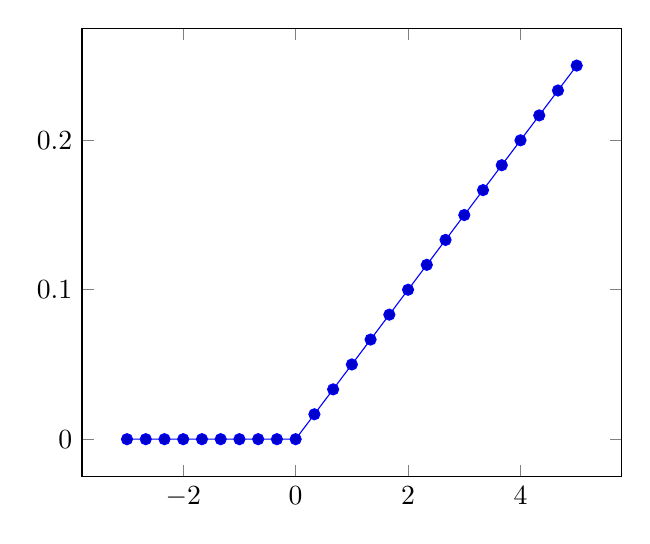
\begin{tikzpicture}
            \begin{axis}[
                domain=-3:5,
            ]
                \addplot{
                    ifthenelse(
                        x<0,            % if
                        0,              % then
                        0.05*x           % else
                    )
                };
            \end{axis}
        \end{tikzpicture}
    \end{center}
    \vspace{-0.2cm}
    \caption{修正线性单元和$\alpha=0.05$的leaky修正线性单元}
    \label{ReLU20200203001}
    \end{figure}
    \item \textbf{卷积}将输入图像放进一组卷积过滤器, 每个过滤器激活图像中的某些特征.
\end{itemize}
%%%%%%%%%%%%%%%%%%%%%%%%%%% M 代码  %%%%%%%%%%%%%%%%%%%%%%%%%%%
\lstinputlisting[language=matlab, caption={平均池化操作函数averagePooling2dLayer}]{code/averagePooling.m}
%%%%%%%%%%%%%%%%%%%%%%%%%%% M 代码  %%%%%%%%%%%%%%%%%%%%%%%%%%%
%%%%%%%%%%%%%%%%%%%%%%%%%%% M 代码  %%%%%%%%%%%%%%%%%%%%%%%%%%%
\lstinputlisting[language=matlab, caption={最大池化操作函数maxPooling2dLayer}]{code/maxPooling.m}
%%%%%%%%%%%%%%%%%%%%%%%%%%% M 代码  %%%%%%%%%%%%%%%%%%%%%%%%%%%
\begin{example}
卷积中的\href{https://blog.csdn.net/weicao1990/article/details/80282837}{滑动步长}是另一个构建卷积神经网络的基本操作.

1) 对默认滑动步长为1, 取左上方的$3\times 3$区域的元素的乘积, 再加起来, 卷积结果的第一个位置(1,1)为91.
%\begin{figure}[H]
%    \centering
%    \includegraphics[width=0.86\textwidth]{1e7180cfff7e697ef0.png}
%\end{figure}
\begin{align*}
\begin{array}{|c|c|c|c|c|c|c|}
\hline 2\;\; ^{3} & 3\;\;^{4} & 7\;\;^{4} & 4 & 6 & 2 & 9 \\
\hline 6\;\;^{1} & 6\;\;^{0} & 9\;\;^{9} & 8 & 7 & 4 & 3 \\
\hline 3\;\;^{-1} & 4\;\;^{0} & 8\;\;^{3} & 3 & 8 & 9 & 7 \\
\hline 7 & 8 & 3 & 6 & 6 & 3 & 4 \\
\hline 4 & 2 & 1 & 8 & 3 & 4 & 6 \\
\hline 3 & 2 & 4 & 1 & 9 & 8 & 3 \\
\hline 0 & 1 & 3 & 9 & 2 & 1 & 4 \\
\hline
\end{array}
\;*\;
\begin{array}{|c|c|c|}
\hline 3 & 4 & 4 \\
\hline 1 & 0 & 2 \\
\hline-1 & 0 & 3 \\
\hline
\end{array}
=
\begin{matrix}
91 &-&- \\
-&- &- \\
-&- &-\\
\end{matrix}
\end{align*}

2) 用$3\times 3$的过滤器卷积这个$7\times 7$的图像, 和之前不同的是, 我们把滑动步长设置成了2, 即stride=2.
\begin{align*}
\begin{array}{|c|c|c|c|c|c|c|}
\hline 2 & 3 & 7\;\; ^{3} & 4\;\; ^{4} & 6\;\; ^{4} & 2 & 9 \\
\hline 6 & 6 & 9\;\; ^{1} & 8\;\; ^{0} & 7\;\; ^{2} & 4 & 3 \\
\hline 3 & 4 & 8\;\; ^{-1} & 3\;\; ^{0} & 8\;\; ^{3} & 9 & 7 \\
\hline 7 & 8 & 3 & 6 & 6 & 3 & 4 \\
\hline 4 & 2 & 1 & 8 & 3 & 4 & 6 \\
\hline 3 & 2 & 4 & 1 & 9 & 8 & 3 \\
\hline 0 & 1 & 3 & 9 & 2 & 1 & 4 \\
\hline
\end{array}
\;*\;
\begin{array}{|c|c|c|}
\hline 3 & 4 & 4 \\
\hline 1 & 0 & 2 \\
\hline-1 & 0 & 3 \\
\hline
\end{array}
=
\begin{matrix}
91 &100&- \\
-&- &- \\
-&- &-\\
\end{matrix}
\end{align*}
%\begin{figure}[H]
%    \centering
%    \includegraphics[width=0.86\textwidth]{6d060f10dd7cb586c4.png}
%\end{figure}

现在移动的步长是2, 我们让过滤器跳过2个滑动步长, 注意一下左上角, 这个点移动到其后两格的点, 跳过了一个位置.
然后你还是将每个元素相乘并求和, (1,2)位置卷积的结果是100 .
\begin{align*}
\begin{array}{|l|l|l|l|l|l|l|}
\hline 2 & 3 & 7 & 4 & 6^{3} & 2^{4} & 9^{4} \\
\hline 6 & 6 & 9 & 8 & 7^{1} & 4^{0} & 3^{2} \\
\hline 3 & 4 & 8 & 3 & 8^{-1} & 9^{0} & 7^{3} \\
\hline 7 & 8 & 3 & 6 & 6 & 3 & 4 \\
\hline 4 & 2 & 1 & 8 & 3 & 4 & 6 \\
\hline 3 & 2 & 4 & 1 & 9 & 8 & 3 \\
\hline 0 & 1 & 3 & 9 & 2 & 1 & 4 \\
\hline
\end{array}
\;*\;
\begin{array}{|c|c|c|}
\hline 3 & 4 & 4 \\
\hline 1 & 0 & 2 \\
\hline-1 & 0 & 3 \\
\hline
\end{array}
=
\begin{matrix}
91 &100&83\\
-&- &- \\
-&- &-\\
\end{matrix}
\end{align*}
%\begin{figure}[H]
%    \centering
%    \includegraphics[width=0.86\textwidth]{2ee8aff917acab.png}
%\end{figure}

3) 为了表示方便, 将数据的分割线舍掉. 继续下一个位置的卷集运算, 将蓝色框移动两个步长, (1,3)位置卷积的结果为83.
%\begin{align*}
%\begin{array}{|l|l|l|l|l|l|l|}
%\hline 2 & 3 & 7 & 4 & 6 & 2 & 9 \\
%\hline 6 & 6 & 9 & 8 & 7 & 4 & 3 \\
%\hline 3\;\; ^{3} & 4\;\;^{4} & 8\;\;^{4} & 3 & 8 & 9 & 7 \\
%\hline 7\;\;^{1} & 8\;\;^{0} & 3\;\;^{2} & 6 & 6 & 3 & 4 \\
%\hline 4\;\;^{-1} &2\;\;^{2} & 1\;\;^{3} & 8 & 3 & 4 & 6 \\
%\hline 3 & 2 & 4 & 1 & 9 & 8 & 3 \\
%\hline 0 & 1 & 3 & 9 & 2 & 1 & 4 \\
%\hline
%\end{array}
%\;*\;
%\begin{array}{|c|c|c|}
%\hline 3 & 4 & 4 \\
%\hline 1 & 0 & 2 \\
%\hline-1 & 0 & 3 \\
%\hline
%\end{array}
%=
%\begin{matrix}
%91 &100&83\\
%69&- &- \\
%-&- &-\\
%\end{matrix}
%\end{align*}
\begin{align*}
\begin{tabularx}{0.4\textwidth}{llllllllllll}
2 & 3 & 7 & 4 & 6 & 2 & 9 \\
6 & 6 & 9 & 8 & 7 & 4 & 3 \\
\cellcolor{intnull} {3\;\; $^{3}$} & \cellcolor{intnull} {4\;\;$^{4}$} & \cellcolor{intnull} {8\;\;$^{4}$} & 3 & 8 & 9 & 7 \\
\cellcolor{intnull} {7\;\;$^{1}$} &\cellcolor{intnull} {8\;\;$^{0}$} & \cellcolor{intnull} {3\;\;$^{2}$} & 6 & 6 & 3 & 4 \\
\cellcolor{intnull} {4\;\;$^{-1}$} &\cellcolor{intnull} {2\;\;$^{2}$} & \cellcolor{intnull} {1\;\;$^{3}$} & 8 & 3 & 4 & 6 \\
3 & 2 & 4 & 1 & 9 & 8 & 3 \\
0 & 1 & 3 & 9 & 2 & 1 & 4 \\
\end{tabularx}
\;\cellcolor{intnull} {*}\;
\begin{tabularx}{0.15\textwidth}{llllllllllll}
3 & 4 & 4 \\
1 & 0 & 2 \\
-1 & 0 & 3 \\
\end{tabularx}
\cellcolor{intnull} {=}\;\;
\begin{matrix}
91 &100&83\\
69&- &- \\
-&- &-\\
\end{matrix}
\end{align*}

%\begin{figure}[H]
%    \centering
%    \includegraphics[width=0.86\textwidth]{54a3b259569f45.png}
%\end{figure}
4) 以此类推, 继续以步长2移动, 会得到91, 127, 最后一行分别是44, 72, 74.
%\begin{figure}[H]
%    \centering
%    \includegraphics[width=0.86\textwidth]{c4b80789d46ed.png}
%\end{figure}

例子用$3\times 3$的矩阵卷积一个$7\times 7$的矩阵, 得到一个$3\times 3$的输出.
输入和输出的维度是由公式 \eqref{AIC7} 决定的.
如果你用一个$N_2\times N_2$的过滤器卷积一个$N_1\times N_1$的图像, 填充数为$P$, 滑动步长为$S$, $3\times 3$的输出变为
\begin{align}\label{AIC7}
    \left\lfloor\frac{N_1+2P-N_2}{S}+1\right\rfloor \times \left\lfloor\frac{N_1+2P-N_2}{S}+1\right\rfloor
          \Rightarrow \left\lfloor\frac{7+0-3}2+1\right\rfloor\times\left\lfloor\frac{7+0-3}2+1\right\rfloor=3\times 3.
\end{align}
\vspace{-0.2cm}
\end{example}
\begin{remark}
滑动步长stride是图像处理中常用的概念.
\begin{example}
    一行有 11 个像素(Width = 11)的图像, 32 位(每个像素 4 字节), $\textup{Stride}= 11 \times 4 = 44$.
\vspace{-0.2cm}
\end{example}
\end{remark}

如果遇到商不是一个整数的情况, 可以向下取整, 这也叫做对进行地板除 (floor), 这意味着向下取整到最近的整数.
这个原则实现的方式是, 你只在蓝框完全包括在图像或填充完的图像内部时, 才对它进行运算.
如果有任意一个蓝框移动到了外面, 就不要进行相乘操作, 这是一个惯例.
$3\times 3$的过滤器必须完全处于图像中或者填充之后的图像区域内才输出相应结果, 这就是惯例.
因此正确计算输出维度的方法是向下取整, 保证结果是整数.

\begin{example}
一行有 11 个像素(Width = 11), 对一个 24 位(每个像素 3 字节)的图像, 按 4 字节对齐, 滑动步长$\textup{Stride} = 11 \times 3 + 3 = 36$.
手动计算 Stride值的步骤:

1) 滑动步长$\textup{Stride} = \textup{每像素占用的字节数(像素位数/8)} \times \textup{Width}$;

2) 如果滑动步长 Stride 不是 4 的倍数, 那么滑动步长 $\textup{Stride} = \textup{Stride} + (4 - \textup{Stride}\, \textup{mod}\, 4)$;
\vspace{-0.2cm}
\end{example} 

总结一下维度情况, 如果你有一个$M\times N_1$的矩阵或者$M\times N_1$的图像, 与一个$N_2\times N_2$的矩阵卷积, 或者说$N_2\times N_2$的过滤器. Padding是$P$, 滑动步长为$S$, 输出尺寸为
\begin{align*}
    \left\lfloor\frac{N_1+2 P-N_2}{S}+1\right\rfloor \quad \times \quad\left\lfloor\frac{N_1+2 P-N_2}{S}+1\right\rfloor.
\end{align*}
选择所有的数使结果是整数是不错的选择, 尽管只要向下取整也就可以.
\begin{example}
自己选择一些参数, 验证卷积输出.
\begin{align*}
\begin{array}{|c|c|c|c|c|c|}
\hline 2\;\;^{7} & 3\;\;^{2} & 7\;\;^{5} & 4 & 6 & 2 \\
\hline 6\;\;^{9} & 6\;\;^{0} & 9\;\;^{4} & 8 & 7 & 4 \\
\hline 3\;\;^{-1} & 4\;\;^{1} & 8\;\;^{3} & 3 & 8 & 9 \\
\hline 7 & 8 & 3 & 6 & 6 & 3 \\
\hline 4 & 2 & 1 & 8 & 3 & 4 \\
\hline 3 & 2 & 4 & 1 & 9 & 8 \\
\hline
\end{array}
\;*\;
\begin{array}{|c|c|c|}
\hline 7 & 2 & 5 \\
\hline 9 & 0 & 4 \\
\hline-1 & 1 & 3 \\
\hline
\end{array}
=?
\end{align*}
\end{example}
%\begin{figure}[H]
%    \centering
%    \includegraphics[width=0.86\textwidth]{962516fc6e636830a.png}
%\end{figure}

这里有一个关于互相关和卷积的技术性建议, 这不会影响到你构建卷积神经网络的方式, 但取决于你读的是数学教材还是信号处理教材, 在不同的教材里符号可能不一致.
\begin{remark}
冈萨雷斯的《数字图像处理》对相关与卷积有详细的介绍.
如果你看的是一本典型的数学教科书, 那么卷积的定义是做元素乘积求和, 实际上还有一个步骤是你首先要做的, 也就是在把这个$6\times 6$的矩阵和$3\times 3$的过滤器卷积之前,
首先你将$3\times 3$的过滤器沿水平和垂直轴翻转(旋转180$^\circ$), 即
\begin{align*}
\left[\begin{array}{ccc}
3 & 4 & 5 \\
1 & 0 & 2 \\
-1 & 9 & 7
\end{array}\right]\rightarrow\left[\begin{array}{crr}
7 & 2 & 5 \\
9 & 0 & 4 \\
-1 & 1 & 3
\end{array}\right].
\end{align*}
这相当于将$3\times 3$的过滤器做了个镜像, 在水平和垂直轴上, 此处应该是先顺时针旋转90得到如下矩阵
\begin{align*}
\left[\begin{array}{ccc}
-1 & 1 & 3 \\
9 & 0 & 4 \\
7 & 2 & 5
\end{array}\right]
\end{align*}
再水平翻转得到
\begin{align*}
\left[\begin{array}{ccc}
7 & 2 & 5 \\
9 & 0 & 4 \\
-1 & 1 & 3
\end{array}\right].
\end{align*}
然后你再把这个翻转后的矩阵复制到这里(左边的图像矩阵), 你要把这个翻转矩阵的元素相乘来计算输出的$4\times 4$矩阵左上角的元素,
9个数字依次平移一个位置, 再平移一格, 以此类推.
\end{remark}
\begin{remark}
    定义上述卷积运算时, 我们跳过了这个镜像操作. 从技术上讲, 我们实际上做的, 我们在前面视频中使用的操作, 有时被称为互相关而不是卷积.
    但在深度学习文献中, 按照惯例, 我们将这(不进行翻转操作)叫做卷积操作 (CS230课程,吴恩达, K. Katanforoosh).
\end{remark}

按照机器学习的惯例, 通常不进行翻转操作. 从技术上说, 这个操作可能叫做互相关更好.
但在大部分的深度学习文献中都把它叫做卷积运算.
很多机器学习的文献把这种运算叫做卷积运算, 不用翻转操作.

事实证明在信号处理中或某些数学分支中, 在卷积的定义包含翻转, 使得卷积运算符拥有这个性质, 即, 这在数学中被称为结合律.
这对于一些信号处理应用来说很好, 但对于深度神经网络来说它真的不重要, 因此省略了这个双重镜像操作, 就简化了代码, 并使神经网络也能正常工作.
大多数人都叫它卷积, 尽管数学家们更喜欢称之为互相关, 这不会影响你的编程练习和实践, 也不影响你理解深度学习.
%%%%%------------------------------------------------------------------
\subsubsection{高维卷积操作——3D卷积}
描述一个二维矩阵,使用行和列. 三维的,使用通道、行和列. 四维则多了一个参数batch.
四个维度(批次、通道、行和列)的逻辑顺序则和数据格式有关,常见的有 \href{https://mp.weixin.qq.com/s/I4Q1Bv7yecqYXUra49o7tw?}{NHWC和NCHW}:

假设过滤器窗口是 $3\times 3\times 3$(其中一个3代表了in\_depth).
有四个这样的窗口,
用于提取同一个图片的四个属性 (out\_depth指定,深度对应输出Out channel 0...3).
那么, 针对图片里面的某个 Batch (譬如Batch 0),其处理流程如下:
%%%%%%%%%%%%%%%%%%%%%%%%%%%%%%%%%%%%%%%%%%
\begin{figure}[H]
\centering
\includegraphics[width=\textwidth]{20190322141457724.PNG}
\caption{深度卷积示意图}
\label{20190322141457724}
\vspace{-0.4cm}
\end{figure}
\vspace{-0.4cm}
%%%%%-----------------------------------------------------
\subsubsection{池化操作}
\textbf{池化}是卷积神经网络中一个重要的概念, 通过执行非线性下采样, 减少网络需要学习的参数个数, 去除冗余信息的同时保留关键信息, 从而简化输出.

池化操作主要有两种方式( ICSIPA 2011 \cite{Nagi2011-6144164}), 一种是平均池化(Average Pooling), 即对邻域内的特征点求平均; 另一种是最大池化(Max Pooling), 即对邻域内的特征点取最大.
最大池化 (Max pooling) 是将输入的图像划分为若干个矩形区域, 对每个子区域输出最大值.
直觉上, 这种机制能够有效地原因在于, 在发现一个特征之后, 它的精确位置远不及它和其他特征的相对位置的关系重要.
池化层会不断地减小数据的空间大小, 因此参数的数量和计算量也会下降, 这在一定程度上也控制了过拟合.
通常来说, CNN的卷积层之间都会周期性地插入池化层.

\ding{171} \href{https://blog.csdn.net/tianwenbo6666/article/details/104349425}{池化(Pooling)} 实际上是一种形式的采样方法.
池化会压缩输入的特征图, 减少数据的特征和参数个数, 进而简化了卷积网络计算时的复杂度;另一方面保持了特征的某种不变性(旋转、平移、伸缩等)
\begin{tcolorbox}[title=池化层]
池化层通常会分别作用于每个输入的特征并减小其大小.
当前最常用形式的池化层是每隔2个元素从图像划分出$2\times 2$的区块, 然后对每个区块中的4个数取最大值.
这将会减少75\%的数据量.
\end{tcolorbox}
%\begin{figure}[H]
%    \centering
%    \includegraphics[width=0.7\textwidth]{Pooling14827576.png}
%    \vspace{-0.5cm}
%    \caption{池化结果}
%    \label{Pooling14827576}
%\end{figure}
池化结果如式 \eqref{AIC7Pooling747}.
\begin{align}\label{AIC7Pooling747}
\begin{tabularx}{0.25\textwidth}{llllllllllll}
\cellcolor{intnull} {1}&\cellcolor{intnull} { 0} & \cellcolor{intdrei}{2} & \cellcolor{intdrei}{3} \\
\cellcolor{intnull} {4} &\cellcolor{intnull} { 6} & \cellcolor{intdrei}{6} & \cellcolor{intdrei}{8} \\
\cellcolor{intdrei}{3} & \cellcolor{intdrei}{1} &\cellcolor{intnull} { 1} &\cellcolor{intnull} { 0 }\\
\cellcolor{intdrei}{1} & \cellcolor{intdrei}{2} &\cellcolor{intnull} { 2} &\cellcolor{intnull} { 4}
\end{tabularx}
\;\cellcolor{intnull} {\rightarrow}\quad
\begin{tabularx}{0.15\textwidth}{llllllllllll}
\cellcolor{intnull} {6} & \cellcolor{intdrei}{8} \\
\cellcolor{intdrei}{3} & \cellcolor{intnull} {4}\\
\end{tabularx}
\end{align}
池化方法特征提取误差主要来自两个部分:
一是, 邻域大小受限造成了估计值方差增大;
二是, 卷积层参数误差造成了估计均值的偏移.
一般来说, 在图像研究领域, 对图像进行平均池化操作能减少第一种误差, 同时更多地保留图像的背景信息;
而另一方面, 最大池化能减小第二种误差, 更多地保留纹理信息.
因此在进行卷积神经网络结构设计时, 这两种池化方式往往交替使用.

池化操作后的结果相比其输入缩小了. 池化层的引入是仿照人的视觉系统对视觉输入对象进行降维和抽象.
池化层有如下三个功效:
\begin{itemize}
    \item 特征不变形:池化操作时, 模型更加关注是否存在某些特征而不是特征具体的位置.
    \item 特征降维:池化相当于在空间范围内做了维度约减, 从而使模型可以抽取更加广范围的特征.
            同时减小了下一层的输入大小, 进而减少计算量和参数个数.
    \item 在一定程度上防止过拟合, 更方便优化.
\end{itemize}
%%%%%------------------------------------------------------------------
\subsubsection{激活函数和层范数}
\textbf{修正线性单元} (ReLU) 通过将负值映射到零和保持正数值, 实现更快、更高效的训练.
CNN的卷积、池化和修正单元三种操作在几十层或几百层上反复进行, 每一层都学习检测不同的特征.
\href{https://dashee87.github.io/deep\%20learning/visualising-activation-functions-in-neural-networks/}{在线绘制各类激活函数网站}.
\begin{remark}
Leaky ReLU激活函数是在声学模型 (2013) 中提出的, 给所有负值赋予一个非零斜率$\alpha=\frac 1 {a_i},\, a_i\in (1,\infty)$.
\end{remark}
\begin{remark}
    CELU \cite{hendrycks2016gelu} 定义为
\begin{align}
    CELU (x)=\max (0,x)+\min (0,\alpha (\exp (x/\alpha)-1)), x\in \mathbb R, \alpha> 0.
\end{align}
\end{remark}
\begin{remark}
    高斯线性误差单元 (GELU), 是高性能神经网络的一种激活函数. GELU 的非线性体现在它的随机正则化算子会随机地应用恒等映射和零映射到神经元的输入上.
GELU 的非线性权重输入由幅值决定, 不同于 ReLUs 中由符号决定.
\begin{align}
    \operatorname{GELU} (x)=x P (X \leq x)=x \Phi (x).
\end{align}
使用下式可以逼近GELU
\begin{align}
    0.5 x\left (1+\tanh \left[\sqrt{2 / \pi}\left (x+0.044715 x^{3}\right)\right]\right).
\end{align}
或者
\begin{align}
    x \sigma (1.702 x).
\end{align}
\end{remark}

Bent-identity \index{激活函数}
\begin{align}
    f (x) = \frac{\sqrt{x^2 + 1} - 1}{2} +x.
\end{align}
关于激活函数PReLU, ELU和SELU的有用性质以及在 CIFAR-10的实验结果  \cite{Godfrey2019-9846}.

Rothaus在1976年提出.因为Bent函数既是非线性度最优的布尔函数, 介于 Identity 与 ReLU 之间的一种折衷选择.
它允许非线性行为, 尽管其非零导数有效提升了学习并克服了与 ReLU相关的静默神经元的问题.
由于其导数可在 1 的任意一侧返回值, 因此它可能容易受到梯度爆炸和消失的影响.

\href{https://arxiv.org/pdf/1901.05894.pdf}{LiSHT (Linearly Scaled Hyperbolic Tangent) 函数}:
\begin{align}
    \phi (x)=x \cdot g (x),\, g (x)=\operatorname{Tanh} (x)=\frac{\exp ^{x}-\exp ^{-x}}{\exp ^{x}+\exp ^{-x}}.
\end{align}

Swish activation 函数 \cite{Ramachandran2018}
\begin{align}
    y (x)=x /\left (1+e^{-x}\right).
\end{align}

\href{https://arxiv.org/pdf/1808.00783.pdf}{Exponential Linear Sigmoid SquasHing} \cite{BasiratPeterandRoth2019}.

分段激活函数综合使用了 Swish 和 Sigmoid 激活函数, 正部  ELU 使用了Swish, 且在它的负部使用了 Sigmoid 激活函数.
对于 Swish, Sigmoid改善了信息的流动性, Linear 能够避免梯度消失, 这也是设计 \href{https://workshops.aapr.at/wp-content/uploads/2019/05/ARW-OAGM19_41.pdf}{ELiSH} 的初衷.
\begin{align}
    y (x)=\left\{\begin{array}{ll}
        x /\left (1+e^{-x}\right), & x \geq 0 \\
        \left (e^{x}-1\right) /\left (1+e^{-x}\right), & x<0
    \end{array}\right..
\end{align}

HardELiSH 的负部是 HardSigmoid 和 ELU 的乘积, 正部使用了 HardSigmoid 和 Linear 的乘积:
\begin{align}
    y (x)=\left\{
    \begin{array}{ll}
        x \times \max (0, \min (1, (x+1) / 2)), & x \geq 0 \\
        \left (e^{x}-1\right) \times \max (0, \min (1, (x+1) / 2)), & x<0
    \end{array}
    \right..
\end{align}

逐点定义的 Soft shrinkage 函数:
\begin{align}
\textup{Soft Shrinkage} (x)=
\left\{
\begin{array}{ll}
    x-\lambda, & \textup{若} x>\lambda \\
    x+\lambda, & \textup{若} x<-\lambda \\
    0,         & \textup{其他}
\end{array}
\right.
\end{align}
参数默认是$\lambda=0.5$.

Softsign

\begin{align}
    \operatorname{Soft} \operatorname{Sign} (x)=\frac{x}{1+|x|}.
\end{align}

Tanhshrink

\begin{align}
    \operatorname{Tanhshrink} (x)=x- \operatorname{Tanh} (x).
\end{align}

Softmin

\begin{align}
    \operatorname{Softmin}\left (x_{i}\right)=\frac{\exp \left (-x_{i}\right)}{\sum_{j} \exp \left (-x_{j}\right)}.
\end{align}

Softmax

\begin{align}
    \operatorname{Softmax}\left (x_{i}\right)=\frac{\exp \left (x_{i}\right)}{\sum_{j} \exp \left (x_{j}\right)}.
\end{align}

LogSoftmax

\begin{align}
    \log \operatorname{Softmax}\left (x_{i}\right)=\log \left (\frac{\exp \left (x_{i}\right)}{\sum_{j} \exp \left (x_{j}\right)}\right).
\end{align}


\href{https://pytorch.org/docs/stable/nn.html#torch.nn.Softshrink}{AdaptiveLogSoftmaxWithLoss}

\begin{align}
    y=\frac{x-\mathrm{E}[x]}{\sqrt{\mathrm{Var}[x]+\epsilon}}  \gamma+\beta.
\end{align}

BatchNorm1d

\begin{align}
    y=\frac{x-\mathrm{E}[x]}{\sqrt{\mathrm{Var}[x]+\epsilon}}  \gamma+\beta.
\end{align}

BatchNorm2d

\begin{align}
    y=\frac{x-\mathrm{E}[x]}{\sqrt{\operatorname{Var}[x]+\epsilon}}  \gamma+\beta.
\end{align}

BatchNorm3d

\begin{align}
    y=\frac{x-\mathrm{E}[x]}{\sqrt{\mathrm{Var}[x]+\epsilon}}  \gamma+\beta.
\end{align}

GroupNorm

\begin{align}
    y=\frac{x-\mathrm{E}[x]}{\sqrt{\mathrm{Var}[x]+\epsilon}}  \gamma+\beta.
\end{align}

SyncBatchNorm

\begin{align}
    y=\frac{x-\mathrm{E}[x]}{\sqrt{\mathrm{Var}[x]+\epsilon}}  \gamma+\beta.
\end{align}

InstanceNorm1d

\begin{align}
    y=\frac{x-\mathrm{E}[x]}{\sqrt{\operatorname{Var}[x]+\epsilon}}  \gamma+\beta.
\end{align}

SoftExponential
\begin{align}
  f (\alpha, x)=\left\{
  \begin{array}{ll}
    {-\frac{\ln (1-\alpha (x+\alpha))}{\alpha}}, & {\textup {当} \alpha<0} \\
    {x}, & {\textup {当} \alpha=0} \\
    {\frac{e^{\alpha x}-1}{\alpha}+\alpha}, & {\textup {当} \alpha>0}
\end{array}\right.,
x\in (-\infty, \infty).
\end{align}

InstanceNorm3d

\begin{align}
    y=\frac{x-\mathrm{E}|x|}{\sqrt{\mathrm{Var}[x]+\epsilon}}  \gamma+\beta.
\end{align}

LayerNorm

\begin{align}
    y=\frac{x-\mathrm{E}[x]}{\sqrt{\mathrm{Var}[x]+\epsilon}  \gamma+\beta}.
\end{align}

LocalResponseNorm

\begin{align}
    b_{c}=a_{c}\left (k+\frac{\alpha}{n} \sum_{c^{\prime}=\max (0, c-n / 2)}^{\min (N-1, c+n / 2)} a_{c^{\prime}}^{2}\right)^{-\beta}.
\end{align}

\href{http://www.gabormelli.com/RKB/Inverse_Square_Root_Unit_ (ISRU)_Activation_Function}{ISRU (Inverse Square Root Unit)} \cite{BradCarlile2017}
\begin{align}
    f (x)=\frac{x}{\sqrt{1+\alpha x^{2}}}, x\in \left (-\frac{1}{\sqrt{\alpha}}, \frac{1}{\sqrt{\alpha}}\right).
\end{align}

Inverse square root linear unit (ISRLU) \cite{BradCarlile2017}
\begin{align}
f (x)=\left\{\begin{array}{ll}
    \frac{x}{\sqrt{1+\alpha x^{2}}}, & \textup{当} x<0 \\
    x, &  \textup{当} x \geq 0
\end{array}\right.,
x\in \left (-\frac{1}{\sqrt{\alpha}}, \infty\right).
\end{align}

SoftPlus \cite{glorot2011}
\begin{align}
    f (x)=\ln \left (1+e^{x}\right), x\in (0, \infty).
\end{align}
%%%%---------------------------------------------------------
\subsection{其他网络结构}
输出序列Multi-layer long short-term memory (LSTM) RNN.
\begin{align}
\begin{array}{l}
{i_{t}=\sigma\left (W_{i i} x_{t}+b_{i i}+W_{h i} h_{ (t-1)}+b_{h i}\right)}, \\
{f_{t}=\sigma\left (W_{i f} x_{t}+b_{i f}+W_{h f} h_{ (t-1)}+b_{h f}\right)}, \\
{g_{t}=\tanh \left (W_{i g} x_{t}+b_{i g}+W_{h g} h_{ (t-1)}+b_{h g}\right)}, \\
{o_{t}=\sigma\left (W_{i o} x_{t}+b_{i o}+W_{h o} h_{ (t-1)}+b_{h o}\right)}, \\
{c_{t}=f_{t}  c_{ (t-1)}+i_{t}  g_{t}}, \\
{h_{t}=o_{t}  \tanh \left (c_{t}\right)}.
\end{array}
\end{align}
其中$h_t$ 是时间$t$时的隐含状态, $c_t$ 是时间$t$时的元胞状态, $x_t$是时间$t$时的输入, $h_{(t-1)}$是时间$t-1$时层的隐含状态, 或者是在初始时刻0的初始隐层状态,
$i_t$, $f_t, g_t, o_t$分别是输入、遗忘、元胞和输出门. $\sigma$ 是sigmoid 函数, $*$ 表示 Hadamard 积. \index{Hadamard 积}
%%%%%%%%%%%%%%%%%%%%%%%%%%%%%%%%%%%%%%%%%%
\begin{figure}[H]
\centering
\includegraphics[width=0.76\textwidth]{CNNStructure1225001.JPG}
\vspace{-0.2cm}
\caption{卷积神经网络}
\label{CNNStructure1225001}
\vspace{-0.4cm}
\end{figure}

\textbf{分类层}在特征检测之后, CNN 的架构转移到分类. 倒数第二层是全连接层 (FCL), 输出$K$维度的向量, 其中$K$是网络能够预测的类数量. 此向量包含任何图像的每个类进行分类的概率. CNN 架构的最后一层使用 softmax 函数提供分类输出.

\begin{remark}
    没有用于选择层数的确切公式. 最好的方法是尝试一些层, 查看工作效果如何, 或者使用预先训练好的网络.
\end{remark}
%%%%%%%%%%%%%%%%%%%%%%%%%%%%%%%%%%%%%%%%%%%
%\begin{figure}[H]
%\centering
%\includegraphics[width=0.76\textwidth]{CNNStructure1225002.JPG}
%\vspace{-0.2cm}
%\caption{卷积神经网络}
%\label{CNNStructure1225002}
%\vspace{-0.4cm}
%\end{figure}

深度学习是机器学习的子类型. 使用机器学习, 您手动提取图像的相关特征. 使用深度学习, 您将原始图像直接馈送给深度神经网络, 该网络自动学习特征.
为了获得最佳结果, 深度学习通常需要成百上千乃至数百万张图像. 而且属于计算密集型, 需要高性能 GPU.
%%%%%%%%%%%%%%%%%%%%%%%%%%%%%%%%%%%%%%%%%%
\begin{figure}[H]
\centering
\includegraphics[width=0.6\textwidth]{AlexNetdemo002.JPG}
\caption{AlexNet的识别对象}
\label{AlexNetdemo002}
\vspace{-0.4cm}
\end{figure}
刚接触深度学习, 快速而轻松的入门方法是使用现有网络, 比如 2012 年首次发布的AlexNet, 已成为研究团体中众所周知的模型.
用一百多万张图像训练好的 CNN.
AlexNet 最常用于图像分类. 它可将图像划分为 1000 个不同的类别, 包括键盘、鼠标、铅笔和其他办公设备, 以及各个品种的狗、猫、马和其他动物.
%%%%%%%%%%%%%%%%%%%%%%%%%%%%%%%%%%%%%%%%%%
\begin{figure}[H]
    \centering
    \includegraphics[width=0.76\textwidth]{CNNMLCompare001.JPG}
    \caption{机器学习和深度学习}
    \label{CNNMLCompare001}
    \vspace{-0.4cm}
\end{figure}
%%%%%%%%%%%%%%%%%%%%%%%%%%%%%%%%%%%%%%%%%%%%
\begin{example}
 (\textbf{AlexNet 的Matlab示例}) 使用 AlexNet 可对任何图像中的对象分类. 本例用它对桌上安装的网络摄像头捕获的图像中的对象分类.
 除了 MATLAB, 还需使用下列工具:
\begin{itemize}
\item Deep Learning Toolbox™;
\item 在 MATLAB 中使用网络摄像头的支持包;
\item 使用 AlexNet 的支持包.
\end{itemize}
在加载 AlexNet 后, 连接到网络摄像头,  拍摄一张实时图像.
\begin{Verbatim}
    camera = webcam; % 连接到摄像头
    nnet = AlexNet; % 加载神经网络
    picture = camera.snapshot;
    % 抓取图片
\end{Verbatim}
接下来, 调整图像大小为 227x227 像素, 即 AlexNet所需的大小.
\begin{Verbatim}
    picture = imresize (picture,[227,227]);
    % 调整图片大小
    AlexNet 现在可对我们的图像分类.
    label = classify (nnet, picture);
    % 对图片分类
    image (picture); % 显示图片
    title (char (label)); % 显示标签
\end{Verbatim}
\vspace{-0.3cm}
\end{example}
上例使用的是现成的网络. 完全不需要做任何修改, 因为 AlexNet 训练所用的图像类似于我们想要分类的图像.

要使用 AlexNet 对未在原有网络中训练的对象分类, 可以通过迁移学习重新训练.
迁移学习是将一个类型问题的知识应用于不同类型但相关的问题的学习方法. \index{迁移学习}
%%%%%%%%%%%%%%%%%%%%%%%%%%%%%%%%%%%%%%%%%%%%
\begin{example}
本例只剪去网络的最后3层, 用新图像重新训练.
%%%%%%%%%%%%%%%%%%%%%%%%%%%%%%%%%%%%%%%%%%
\begin{figure}[H]
\centering
\includegraphics[width=0.76\textwidth]{CNNMatlabGPU001.JPG}
\caption{深度学习和机器学习}
\label{CNNMatlabGPU001}
\end{figure}

如果迁移学习不适合自己的应用场景, 可能需要从头开始训练您自己的网络. 这种方法产生最精确的结果, 但一般需要成百上千张带标签的图像和大量的计算资源.
培训深度学习模型可能需要几小时、几天或几星期, 具体取决于数据量大小, 以及可投入使用的处理能力.
当前, 有三个计算选项: 基于 CPU、基于 GPU 和基于云三种.
选择计算资源是建立工作流程时的重要考虑因素.
\begin{itemize}
\item 基于 CPU 的计算是最简单、最容易得到的选项. 前面所述的示例在CPU 上运算, 只需对使用预先训练网络的简单示例, 一般推荐先使用基于 CPU 的计算.
\item 使用 GPU 可将网络训练时间从几天缩短到几小时. 可以在 MATLAB 中使用 GPU, 无需任何额外编程. 推荐具有 NVIDIA\textcopyright 3.0 以上计算能力的 GPU.
多个 GPU 能更加快地处理速度.
\item 基于云的 GPU 计算意味着不需自行购买和设置硬件, 以及为使用本地 GPU 而编写的 MATLAB 代码; 只需进行一些设置变更, 便可扩展为使用云资源.
\end{itemize}
\vspace{-0.2cm}
\end{example}

通常CNN网络在卷积层之后会接上若干个全连接层, 将卷积层产生的特征图映射成一个固定长度的特征向量.
以AlexNet为代表的经典CNN结构适合于图像级的分类和回归任务, 因为它们最后都期望得到整个输入图像的一个数值描述 (概率).
AlexNet的ImageNet模型输出一个1000维的向量表示输入图像属于每一类的概率 (softmax归一化).
如图 \ref{CNN10-01429-ag}, CNN在第三层后进行了特征融合. 通过最大池化融合了两个数据流, 同时, 进行了批量正则化和 relu层上的卷积运算.
最后, 两个输出进行了整合, 第四层输出形态含有分类结果 \cite{PiramanayagamSaber2018-9591}.
FCN对图像进行像素级的分类, 从而解决了语义级别的图像分割 (语义分割) 问题.
%%%%%%%%%%%%%%%%%%%%%%%%%%%%%%%%%%%%%%%%%%
\begin{figure}[H]
    \centering
    \includegraphics[width=0.76\textwidth]{CNN10-01429-ag.png}
    \caption{CNN第三层后的特征融合. 两个数据流通过最大池化, 批量正则化和 relu层上的卷积. 两个输出的整合以及第四层的输出形态等特征 \cite{PiramanayagamSaber2018-9591}}
    \label{CNN10-01429-ag}
    \vspace{-0.4cm}
\end{figure}

与经典的CNN在卷积层之后使用全连接层得到固定长度的特征向量进行分类 (全联接层+softmax输出) 不同, FCN可以接受任意尺寸的输入图像, 采用反卷积层对最后一个卷积层的特征映射进行上采样,
使它恢复到输入图像相同的尺寸, 从而可以对每个像素都产生了一个预测, 同时保留了原始输入图像中的空间信息, 最后在上采样的特征图上进行逐像素分类.
如图 \ref{CNNfcn320203} 给出了FCN-32学习网络的结构, Unet ushape网络 \ref{CNNUnetushape0203} 以及平直化后的 Unet 学习网络 \ref{CNNUnet0203} .
%%%%%%%%%%%%%%%%%%%%%%%%%%%%%%%%%%%%%%%%%%
\begin{figure}[H]
    \centering
    \includegraphics[width=0.86\textwidth]{fcn32.pdf}
    \caption{FCN-32学习网络}
    \label{CNNfcn320203}
    \vspace{-0.4cm}
\end{figure}

Softmax损失函数的结构如图 \ref{CNNSoftmaxLoss0203}.
%%%%%%%%%%%%%%%%%%%%%%%%%%%%%%%%%%%%%%%%%%
\begin{figure}[H]
    \centering
    \includegraphics[width=0.4\textwidth]{SoftmaxLoss.pdf}
    \caption{Softmax Loss}
    \label{CNNSoftmaxLoss0203}
    \vspace{-0.4cm}
\end{figure}
%%%%%%%%%%%%%%%%%%%%%%%%%%%%%%%%%%%%%%%%%%
\begin{figure}[H]
    \centering
    \includegraphics[width=0.5\textwidth]{Unetushape.pdf}
    \caption{Unet ushape网络}
    \label{CNNUnetushape0203}
    \vspace{-0.4cm}
\end{figure}
%%%%%%%%%%%%%%%%%%%%%%%%%%%%%%%%%%%%%%%%%%
\begin{figure}[H]
    \centering
    \includegraphics[width=0.86\textwidth]{Unet.pdf}
    \caption{Unet 学习网络}
    \label{CNNUnet0203}
    \vspace{-0.4cm}
\end{figure}
VGGNet是牛津大学计算机视觉组和 Google DeepMind 公司的研究员一起研发的深度卷积神经网络 \ref{CNNvgg16020301}.\index{VGGNet}
VGGNet探索了卷积神经网络的深度与其性能之间的关系, 通过反复堆叠$3\times 3$的小型卷积核和$2\times 2$的最大池化层,
VGGNet成功地构筑了 16\textasciitilde 19 层深的卷积神经网络.
VGGNet相比之前最前沿的网络结构, 错误率大幅下降,
VGGNet相关的论文全部使用了$3\times 3$的小型卷积核和$2\times 2$的最大池化核, 通过不断加深网络结构来提升性能.
%%%%%%%%%%%%%%%%%%%%%%%%%%%%%%%%%%%%%%%%%%
\begin{figure}[H]
    \centering
    \includegraphics[width=\textwidth]{vgg16.pdf}
    \caption{vgg-16 网络}
    \label{CNNvgg16020301}\vspace{-0.4cm}
\end{figure}
%%%%%%%%%%%%%%%%%%%%%%%%%%%%%%%%%%%%%%%%%%
\begin{figure}[H]
    \centering
    \includegraphics[width=0.9\textwidth]{CNNvgg16LayerPara.png}
    \caption{vgg-16各层的参数和内存使用情况}
    \label{CNNvgg16LayerPara020302}
    \vspace{-0.4cm}
\end{figure}
%%%%%%%%%%%%%%%%%%%%%%%%%%%%%%%%%%%%%%%%%
\subsection{防止CNN过拟合的方法——diffGrad}
Train CIFAR10 with PyTorch. \href{https://ieeexplore.ieee.org/document/8939562}{diffGrad: An Optimization Method for Convolutional Neural Networks}. IEEE Transactions on Neural Networks and Learning Systems, 2019.
DOI: 10.1109/TNNLS.2019.2955777, 2919-12-23.

DiffGrad是Dubey等人在论文《DiffGrad: CNN的优化器》中介绍的一种新的优化器, 它建立在Adam优化器的基础上, 开发了一种自适应的 ``friction clamp", 并监测梯度的局部变化, 以便自动锁定Adam可以跳过的最优参数值.
通过 ``friction clamping"锁定到最优的最小值: 相比之下, diffGrad监测当前梯度与前一步的即时变化, 并应用自适应 ``friction clamping", 可在梯度变化很小的时候迅速减速, 从而暗示最优解可能就在附近.
diffGrad能够以理想的损失锁定到全局最小值. Adam由于无法及时减速而跳到了更高的局部最小值.
一些论文已经提出了解决已知overshoot问题的解决方案, 但是diffGrad可以稳定地解决它, 还给出了其他几个变量如何应用clamping或friction系数.
\href{https://ieeexplore.ieee.org/document/8939562}{IEEE TNNLS version文献}, 实验室用的框架 \href{https://github.com/kuangliu/pytorch-cifar}{pytorch-cifar}.
%Abstract: Stochastic Gradient Decent (SGD) is one of the core techniques behind the success of deep neural networks. The gradient provides information on the direction in which 函数 has the steepest rate of change. The main problem with basic SGD is to change by equal sized steps for all parameters, irrespective of gradient behavior. Hence, an efficient way of deep network optimization is to make adaptive step sizes for each parameter. Recently, several attempts have been made to improve gradient descent methods such as AdaGrad, AdaDelta, RMSProp and Adam. These methods rely on the square roots of exponential moving averages of squared past gradients. Thus, these methods do not take the advantage of local change in gradients. In this paper, a novel optimizer is proposed based on the difference between the present and the immediate past gradient (i.e., diffGrad). In the proposed diffGrad optimization technique, the step size is adjusted for each parameter in such a way that it should have a larger step size for faster gradient changing parameters and lower step size for lower gradient changing parameters. The convergence analysis is done using the regret bound approach of online learning framework. Rigorous analysis is made in this paper over three synthetic complex non-convex 函数s. The image categorization experiments are also conducted over the CIFAR10 and CIFAR100 datasets to observe the performance of diffGrad with respect to the state-of-the-art optimizers such as SGDM, AdaGrad, AdaDelta, RMSProp, AMSGrad, and Adam. The residual unit (ResNet) based Convolutional Neural Networks (CNN) architecture is used in the experiments. The experiments show that diffGrad outperforms the other optimizers. Also, we showed that diffGrad performs uniformly well on network using different activation 函数s.
%%%%%%%%%%%%%%%%%%%%%%%%%%%%%%%%%%%%%%%
\subsubsection{ShuffleNet}
\begin{tcolorbox}[title=ShuffleNet]
$\bullet$ 逐点分组卷积;

$\bullet$ 通道重排 ( channel shuffle);

$\bullet$ 堆叠地使用瓶颈单元ShuffleNet单.
\end{tcolorbox}
%%%%%%%%%%%%%%%%%%%%%%%%%%%%%%%%%%%%%%%%%%%
%\begin{figure}[H]
%    \centering
%    \includegraphics[width=\textwidth]{RNNAPP2019121500007.PNG}
%    \caption{网络模型参数压缩}
%    \label{RNNAPP2019121500007}\vspace{-0.4cm}
%\end{figure}
%%%%%%%%%%%%%%%%%%%%%%%%%%%%%%%%%%%%%%%%%%
\begin{figure}[H]
    \centering
    \includegraphics[width=0.86\textwidth]{RNNAPP2019121500008.PNG}
    \caption{通道重排和ShuffleNet单元}
    \label{RNNAPP2019121500008}\vspace{-0.4cm}
\end{figure}
%%%%%%%%-------------------------------------------------------------------------------
%%%%%%%%%%%%%%%%%%%%%%%%%%%%%%%%%%%%%%
\subsection{CNN应用场景——计算机视觉问题}

\qquad\ding{172} 图像分类 : 识别出该图像属于哪个类别.

\qquad\ding{173} 目标定位: 在图像分类的基础上,  定位找到对象在图像中的位置.

\qquad\ding{174} 目标检测: 给出在图像内所有该类别的目标和对应的位置.

\qquad\ding{175} 图像分割: 具体到像素级别的图像处理.

\qquad\ding{176} 无人驾驶汽车在接近人行横道线时减速.

\qquad\ding{177} ATM 拒收假钞.

\qquad\ding{178} 智能手机应用程序即时翻译国外路标.

\qquad\ding{179} UCLA 研究人员建造了一种高级显微镜, 能产生高维的数据集, 用来训练深度学习网络, 在组织检体中识别癌细胞.

深度学习特别适合鉴别应用场景, 比如人脸辨识、文本翻译、语音识别以及高级驾驶辅助系统 (包括车道分类和交通标志识别).

先进的工具和技术极大改进了深度学习算法, 达到了很高的水平, 在图像分类上能够超越人类, 能打败世界最优秀的围棋选手, 还能实现语音控制助理功能, 如 Amazon Echo 和 Google Home, 可用来查找和下载您喜欢的新歌.

三个技术助推器让这种精确度成为可能:
\begin{itemize}
\item 大规模带标签的数据集ImageNet 和 PASCAL VoC 等数据集可以免费使用, 对于许多不同类型的对象训练十分有用.
%%%%%%%%%%%%%%%%%%%%%%%%%%%%%%%%%%%%%%%%%%
\begin{figure}[H]
    \centering
    \includegraphics[width=0.76\textwidth]{DNNUlabelSet.JPG}
    \caption{大规模带标签的免费数据集}
    \label{DNNUlabelSet201912250001}
    \vspace{-0.4cm}
\end{figure}
\item 增大的计算能力: 高性能 GPU加快了深度学习所需的海量数据的训练速度, 训练时间从几星期减少到几小时.
%%%%%%%%%%%%%%%%%%%%%%%%%%%%%%%%%%%%%%%%%%
\begin{figure}[H]
    \centering
    \includegraphics[width=0.76\textwidth]{GPUCloud.JPG}
    \caption{算力的规模}
    \label{GPUCloud201912250002}
\end{figure}
\item 由专家构建的预先训练好的模型可以重新训练 AlexNet之类的模型, 使用名为迁移学习的技术执行新识别任务.
虽然使用了 130万张高分辨率图像训练 AlexNet来识别 1000个不同的对象, 但可以使用较小的数据集实现精确的迁移学习.
\end{itemize}
%%%%%%%%%%%%%%%%%%%%%%%%%%%%%%%%%%%%%%%%%%
\begin{figure}[H]
    \centering
    \includegraphics[width=0.76\textwidth]{AleNet130.JPG}
    \caption{迁移学习模型}
    \label{AleNet130201912250003}
\end{figure}
%%%%%%%%%%%%%%%%%%%%%%%%%%%%%%%%%%%%%%%%%%
\begin{figure}[H]
    \centering
    \includegraphics[width=0.76\textwidth]{CNNAPP201912150001.PNG}
    \caption{ AlexNet的目标分割}
    \label{CNNAPP201912150001}
\end{figure}
%%%%%%%%------------------------------------------------------
\subsubsection{CNN解释器在线交互可视化工具}
佐治亚理工的Zijie Wang将CNN拆开, 做了一个CNN在线交互可视化工具,  解释器CNN如何识别人脸、听辨声音.
它用 TensorFlow.js 加载了一个10层的预训练模型, 相当于在你的浏览器上跑一个CNN模型, 只需要打开电脑, 就能了解CNN究竟是怎么回事.

\href{https://poloclub.github.io/cnn-explainer/}{CNN解释器}, \href{https://github.com/poloclub/cnn-explainer}{GitHub代码地址}和论文地址
\href{https://arxiv.org/abs/2004.1500}{《Toric Construction and Chow Ring of Moduli Space of Quasi Maps from $\mathbb P^1$ with Two Marked Points to $\mathbb P^1\times \mathbb P^1$》}
%%%%%%%%%%%%%%%%%%%%%%%%%%%%%%%%%%%%%%%%%%
\begin{figure}[H]
    \centering
    \includegraphics[width=0.6\textwidth]{CNNAPP201912150002.PNG}
    \caption{图像分类 ( AlexNet在ILSVRC-2012测试图像上预测的top-5标签)}
    \label{CNNAPP201912150002}
    \vspace{-0.4cm}
\end{figure}
%%%%%%%%%%%%%%%%%%%%%%%%%%%%%%%%%%%%%%%%%%
\begin{figure}[H]
    \centering
    \includegraphics[width=0.6\textwidth]{CNNAPP201912150003.PNG}
    \caption{目标检测 ( Faster R-CNN在COCO数据集的检测结果)}
    \label{CNNAPP201912150003}
    \vspace{-0.4cm}
\end{figure}
%%%%%%%%%%%%%%%%%%%%%%%%%%%%%%%%%%%%%%%%%%
\begin{figure}[H]
    \centering
    \includegraphics[width=0.76\textwidth]{CNNAPP201912150004.PNG}
    \caption{图像分割 ( SegNet模型分割结果)}
    \label{CNNAPP201912150004}
    \vspace{-0.4cm}
\end{figure}
%%%%%%%%%%%%%%%%%%%%%%%%%%%%%%%%%%%%%%%%%%
\begin{figure}[H]
    \centering
    \includegraphics[width=0.76\textwidth]{CNNAPP201912150005.PNG}
    \caption{人脸识别 ( DeepFace模型)}
    \label{CNNAPP201912150005}
    \vspace{-0.4cm}
\end{figure}
%%%%%%%%------------------------------------------------------
\subsubsection{卷积编译码网络学习语义图形实现水稻自动除草}
该方法将语义图形用于数据注释并结合高级编译码网络, 实现\href{https://doi.org/10.3389/fpls.2019.01404}{稻田中自动作物行和杂草检测} (\cite{Adhikari-2019}, 2019.10), 主要内容如下:
%%%%%%%%%%%%%%%%%%%%%%%%%%%%%%%%%%%%%%%%%%
\begin{figure}[H]
    \centering
    \includegraphics[width=0.76\textwidth]{CCNshuidao20191216181023.jpg}
    \caption{训练深度神经网络的方法使用语义图形来学习作物行的概念}
    \label{CCNshuidao20191216181023}
    \vspace{-0.4cm}
\end{figure}
杂草是农场侵略者, 与作物争夺营养及其他资源, 造成作物产量降低.
化学品的大量使用能够控制杂草, 但会对人类健康和环境造成意想不到的后果.
思路就是找到一种新型神经网络训练方法, 该方法将语义图形用于数据注释并结合高级编译码网络, 实现稻田中自动作物行和杂草检测.
利用检测到的作物行指导自动除草机器人行间除草, 而杂草检测则使自动行内除草成为可能. 提出的训练深度神经网络的方法使用语义图形来学习作物行的概念.
%%%%%%%%%%%%%%%%%%%%%%%%%%%%%%%%%%%%%%%%%%
\begin{figure}[H]
    \centering
    \includegraphics[width=0.6\textwidth]{CCNshuidao20191216181108.jpg}
    \caption{稻田数据集上使用语义扩展跳过网络学习语义线的定性结果}
    \label{CCNshuidao20191216181108}
    \vspace{-0.4cm}
\end{figure}

直观的稻谷数据集的语义图形.

所提出的数据注释方法语义图形直观, 并且注释所需目标的工作量很少. ``extended skip network"是一种改进的深卷积编译码神经网络, 用于语义图形的高效学习.
研究结果表明, 在水稻行和杂草检测中, 相对于基线网络, 联合平均交叉数 (mIoU)分别增加了6.29%和6.14%.
并且与当前流行的基于边界框的对象检测方法相比, 该方法也使得 mIoU 增加了3.56\%, 具有更高的召回率.
图 \ref{CCNshuidao20191216181108} 给出了在稻田数据集上使用拟议的扩展跳过网络学习语义线的定性结果.
图 \ref{CCNshuidao20191216181137} 给出了在稻谷数据集上使用拟议的卷积编码器/解码器网络学习语义图形的定性结果.
%%%%%%%%%%%%%%%%%%%%%%%%%%%%%%%%%%%%%%%%%%
\begin{figure}[H]
    \centering
    \includegraphics[width=0.6\textwidth]{CCNshuidao20191216181137.jpg}
    \caption{稻谷数据集上使用语义卷积编码器/解码器网络学习语义图形的定性结果}
    \label{CCNshuidao20191216181137}
    \vspace{-0.4cm}
\end{figure}
%%%%%%%%------------------------------------------------------
\section{图卷积神经网络}
\href{https://github.com/zggl/planetoid}{图卷积网络}由University of Amsterdam的Thomas N. Kipf提出, 2020年博士毕业, \href{https://arxiv.org/abs/1609.02907}{SEMI-SUPERVISED CLASSIFICATION WITH
GRAPH CONVOLUTIONAL NETWORKS}, 纽约大学, 纽约大学上海分校, AWS上海研究院以及 AWS MXNet Science Team 共同开发的 \href{https://www.dgl.ai/}{图神经网络的框架}

阿里如何把图卷积网络用于闲鱼的垃圾评论过滤. 目前该系统已经部署到了闲鱼使用环境中, 它每天能处理百万级的闲鱼评论, 并在其他强有力的深度学习模型基础上, 额外筛选出一千多条非常隐秘的垃圾评论.
基于图卷积的垃圾信息筛选是一种非常通用的思想, 它的应用范围远不止垃圾评论过滤, 淘宝信息的知识产权保护、淘宝商品管控和用户恶意评价等方面都可以采用.
GAS 的整体流程是 如图 \ref{GNNGAS20191216202234}, 模型会从左侧图抽取出表示商品、用户和评论的信息, 从右侧抽取出类似评论表示的意义. 最后结合这些信息进行分类, 模型就能很好地识别垃圾信息了.
%%%%%%%%%%%%%%%%%%%%%%%%%%%%%%%%%%%%%%%%%%
\begin{figure}[H]
    \centering
    \includegraphics[width=0.76\textwidth]{GNNGAS20191216202234.jpg}
    \caption{基于GCN的垃圾信息过滤系统 (GAS)}
    \label{GNNGAS20191216202234}
    \vspace{-0.4cm}
\end{figure}
%%%%%%%%%%%%%%%%%%%%%%%%%%%%%%%%%%%%%%%%%

百度全球顶会论文复现营202007-GAN
\begin{itemize}
\item \href{https://arxiv.org/abs/1809.11096}{Large scale GAN training for high fidelity natural image synthesis}
\item \href{https://arxiv.org/abs/1910.12713v1c}{Few-shot Video-toVideo Synthesis}
\item \href{https://arxiv.org/abs/1912.01865}{StarGAN v2: Diverse Image Synthesis for Multiple Domains}
\item \href{https://arxiv.org/abs/1907.10830?context=cs.CV}{U-GAT-IT: Unsupervised Generative Attentional Networks with Adaptive Layer-Instance Normalization for Image-to-Image Translation}
\item \href{http://papers.nips.cc/paper/8935-first-order-motion-model-for-image-animation}{First Order Motion Model for Image Animation}
\end{itemize}

图卷积的核心思想是希望利用近邻节点的信息进行聚合而生成当前节点的新表征, 这样的节点表示可以进一步用于下游任务.
如果我们直接从核心表达式出发, 跳过推导过程, 其实能更容易地理解. 如下所示为两层图卷积网络之间的传播方法, 它看起来只不过比常规的神经网络多了 $\tilde D$ 与$\tilde A$这几项.
\begin{align}
    H^{ (l+1)}=\sigma\left (\tilde{D}^{-\frac{1}{2}} \tilde{A} \tilde{D}^{-\frac{1}{2}} H^{ (l)} W^{ (l)}\right).
\end{align}
如果我们的图有 $n $个节点, 那么节点与节点之间的关系可以用$n\times n$的邻接矩阵表示, 它再加上由节点特征向量组成的矩阵$H$就是图卷积的输入.
在上式中, $\tilde A$以及$\tilde D$就是由邻接矩阵算出来的结果, 它对于同一张图是不变的, 因此可以预先计算好.
现在, 剩下的 $H\times W$ 就是输入Embedding H经过一层全连接层了, 以这样方式进行层级传播的卷积网络就是图卷积, 我们可以将传播理解为每个节点拿到邻居节点信息, 并聚合到自身嵌入向量上.
如图 \ref{GNNGAS20191216202340} 所示, 图卷积网络的输入是表示节点及边的特征向量, 经过一系列隐藏层的变换, 可以计算出每个节点的深度表征.
这样的 $Z$再来做预测或生成就会非常有效. 直观而言, 图卷积将图片的 RGB 像素值替换成节点特征, 并且通过边的关系引入了邻居的概念, 完成卷积运算.
%%%%%%%%%%%%%%%%%%%%%%%%%%%%%%%%%%%%%%%%%%
\begin{figure}[H]
    \centering
    \includegraphics[width=0.76\textwidth]{GNNGAS20191216202340.jpg}
    \caption{图卷积网络的输入输出结构}
    \label{GNNGAS20191216202340}
    \vspace{-0.4cm}
\end{figure}
%%%%%%%%%%%%%%%%%%%%%%%%%%%%%%%%%%%%%%%%%

\textbf{异构图上的图卷积}

阿里 GAS 一共有两种输入图, 它们分别用来表示局部信息与全局信息. 首先我们看看异构图, 一般只要边的种类加上节点的种类大于 2, 我们就可以称之为异构图.
如 \ref{GNNGAS20191216202359} 所示闲鱼图为一个标准的异构图, 目前图卷积网络大部分都关注更简单的同构图, 闲鱼图这种异构图很难处理.
从图 \ref{GNNGAS20191216202359} 我们可以看到, 闲鱼 Graph 有商品 $I$ 和用户 $U$ 这两种节点, 它们的边为评论 $E$.
如上, $e_2$,$e_4$ 和 $e_5$ 都是垃圾评论, 它们都来自于同一用户. 利用图来判断垃圾评论, 能利用更多的额外信息, 准确率也会比纯文本好得多.
现在回到图卷积, 一般图卷积的层级可以分为聚合 (aggregation)与结合 (combination)两大操作.
其中 AGG 会聚合邻近节点的嵌入向量, 例如最大池化或基于注意力权重的加权和等.
COMBINE 操作会结合自身的嵌入向量与前面聚合的嵌入向量, 很多 GCN 方法将 COMBINE 操作放到了 AGG 里面.
在阿里的 GAS 中, 研究者使用拼接的方式将信息聚合到边上. 比如说如果 GAS 需要将信息聚合到不同的边 (即评论)上, 那么比较核心的表达式可以写为:
\begin{align}
    h_{e}^{l}=\sigma\left (W_{E}^{l} \cdot A G G_{E}^{l}\left (h_{e}^{l-1}, h_{U (e)}^{l-1}, h_{I (e)}^{l-1}\right)\right),
\end{align}
其中
\begin{align*}
    A G G_{E}^{l}\left (h_{e}^{l-1}, h_{U (e)}^{l-1}, h_{I (e)}^{l-1}\right)=\operatorname{concat}\left (h_{e}^{l-1}, h_{U (e)}^{l-1}, h_{I (e)}^{l-1}\right),
\end{align*}
其中$ h^l$ 表示第 l 层边的隐藏向量, 它需要聚合 l-1 层自身的特征向量以及与它相连的两个节点向量, 聚合的方法是拼接三个向量.
$W^l$表示该神经网络层所需要学习的权重, $\sigma$表示激活函数.
看上去它其实和一般的卷积网络并没有什么差别, 只不过输入都是图的各种信息, 这样也能基于局部上下文判断该评论是否是垃圾评论.
%%%%%%%%%%%%%%%%%%%%%%%%%%%%%%%%%%%%%%%%%%
\begin{figure}[H]
    \centering
    \includegraphics[width=0.6\textwidth]{GNNGAS20191216202359.jpg}
    \caption{图卷积异构网络——闲鱼 Graph}
    \label{GNNGAS20191216202359}
    \vspace{-0.4cm}
\end{figure}
%%%%%%%%%%%%%%%%%%%%%%%%%%%%%%%%%%%%%%%%%
当然上面只是展示了边的聚合案例, 其它节点的 AGG 操作和 COMBINE 运算在原论文中都有详细的介绍.
此外, 如果从异构图卷积网络的输入与输出来考虑,
对于单个用户节点, 输入就是邻近商品节点以及邻近评价边的特征.
%%%%--------------------------------------------------------------------
\begin{example}
    一个用户评论了 10 件商品, 那么每一个商品向量拼接上对应评论向量, 这 10 个特征向量就可以作为输入, 后续图卷积就会对它们进行基于注意力机制的聚合等一系列操作.
\end{example}

\textbf{同构图上的图卷积}

对于闲鱼 Graph 这种大型图, 我们能处理邻近节点这些局部信息, 但与此同时还应该能处理全局信息, 这样才能有效地减轻用户的对抗行为.
为此, 模型应该站在所有评论的角度, 看看与当前相似的评论都是什么样, 它们是不是垃圾评论.
阿里的研究者基于闲鱼 Graph 构建了一种新的 Comment Graph, 它是一种同构图, 每一个节点为评论内容, 节点之间的边为两条评论之间的相似性.
因为相似的评论距离非常近, 因此模型可以考虑与当前评论相近的评论, 从而更好地判断当前评论是不是垃圾评论.

图 \ref{GNNGAS20191216202416} 给出了一小部分 Comment Graph, 如果说局部模型无法根据「add v」判断出意思是加微信, 那么放在 Comment Graph 中就非常明确了, 它与类似的说法都应该被判断为垃圾评论.
%%%%%%%%%%%%%%%%%%%%%%%%%%%%%%%%%%%%%%%%%%
\begin{figure}[H]
    \centering
    \includegraphics[width=0.7\textwidth]{GNNGAS20191216202416.jpg}
    \caption{基于闲鱼 Graph 构建的 同构Comment Graph}
    \label{GNNGAS20191216202416}
    \vspace{-0.4cm}
\end{figure}
%%%%%%%%%%%%%%%%%%%%%%%%%%%%%%%%%%%%%%%%%
简单而言, Comment Graph 的构建主要分为四个步骤: 移除所有重复的评论;
通过词嵌入模型为评论生成嵌入向量; 利用 KNN Graph 算法获得相似的评论对;
移除同一用户提出的评论对, 或者同一卖家提出的评论, 因为之前的闲鱼 Graph 已经考虑了这些信息.
构建了 Comment Graph, 再用图卷积就能抽取节点信息了, 因为每一个节点输出向量都聚合了周围节点的信息, 它就能代表全局上这一些相似评论的意义.
最后, 结合异构图卷积与同构图卷积的结果, 再来做个简单的分类就很合理了.
%%%%%%%%%%%%%%%%%%%%%%%%%%%%%%%%%%%%%%%%%
\section{循环神经网络 (Recurrent Neural Networks, RNN)}
针对对象: 序列数据. 例如文本是字母和词汇的序列; 语音是音节的序列; 视频是图像的序列;
气象观测数据, 股票交易数据等也都是序列数据. RNN 专门解决时间序列问题, 用来提取时间序列信息, 一般放在CNN特征提取层之后.

核心思想: 样本间存在顺序关系, 每个样本和它之前的样本存在关联.
通过神经网络在时序上的展开, 我们能够找到样本之间的序列相关性.
%%%%%%%%%%%%%%%%%%%%%%%%%%%%%%%%%%%%%%%%%%
\begin{figure}[H]
    \centering
    \includegraphics[width=0.76\textwidth]{RNN201912150001.PNG}
    \caption{RNN网络结构按时间展开}
    \label{RNN201912150001}
    \vspace{-0.4cm}
\end{figure}
%%%%%%%%%%%%%%%%%%%%%%%%%%%%%%%%%%%%%%%%%%
%%%%%%%%%%%%%%%%%%%%%%%%%%%%%%%%%%%%%%%%%%
\begin{figure}[H]
    \centering
    \includegraphics[width=0.76\textwidth]{RNNImage191229001.png}
    \caption{RNN网络结构}
    \label{RNNImage191229001}
    \vspace{-0.4cm}
\end{figure}

RNN主要用于序列分类

-情感分类和视频分类序列标记.

-语音标记和命名实体识别序列生成.

-机器翻译和音译.

在循环神经网络中的每个时间步处, 旧信息都会随着当前输入而发生变化.
对于较长的句子, 我们可以想象, 在$t$时间步之后, 存储在$t-k$时间步 ($k\ll t)$的信息会经历一个逐渐转变的过程.
在反向传播过程中, 信息必须流经较长的时间步才能更新网络参数, 以最大程度地减少网络的损失.

考虑一个场景, 在该场景中, 我们需要计算时间步$L$处的网络损失.
假定损失是由于在时间步$S_1$对隐藏表示的错误计算而产生的. $S$处的错误是由于向量$W$的参数不正确造成的. 此信息必须反向传播到$W$, 以便向量可以校正其参数.
\begin{align}
    a_{j}=U x_{j}+W s_{j-1}+b, s_{j}=\sigma\left (a_{j}\right).
\end{align}
%%%%%%%%%%%%%%%%%%%%%%%%%%%%%%%%%%%%%%%%%%
\begin{figure}[H]
    \centering
    \includegraphics[width=0.6\textwidth]{RNNImage191229002.png}
    \caption{RNN权重作用示意图}
    \label{RNNImage191229002}\vspace{-0.4cm}
\end{figure}

为了将信息传播回向量$W$, 我们需要用到链式法则的概念.
简而言之, 链式法则归结为特定时间步的所有隐藏表示的偏导数的乘积.
\begin{align}
    \frac{\partial \mathscr{L}_{t} (\theta)}{\partial W}&=\frac{\partial \mathscr{L}_{t} (\theta)}{\partial s_{t}} \sum_{k=1}^{t} \frac{\partial s_{t}}{\partial s_{k}} \frac{\partial s_{k}}{\partial W}\\
    \frac{\partial s_{t}}{\partial s_{k}}               &=\frac{\partial s_{t}}{\partial s_{t-1}} \frac{\partial s_{t-1}}{\partial s_{t-2}} \frac{\partial s_{t-2}}{\partial s_{t-3}} \cdots \frac{\partial
                                                               s_{k+1}}{\partial s_{k}} \Rightarrow \frac{\partial s_{t}}{\partial s_{k}}=\prod_{j=k+1}^{t} \frac{\partial s_{j}}{\partial s_{j-1}}.
\end{align}

如果我们有超过100个或者更长的序列的隐藏表示, 那么我们必须计算这些表示的乘积来进行反向传播.
假设其中一个偏导数值很大, 那么整个梯度值就会非常大, 从而导致梯度爆炸问题.
如果其中一个偏导数是一个很小的值, 那么整个梯度就会变得更小或消失, 使得网络难以训练, 导致出现梯度消失问题.
由于RNN具有有限的状态大小, 而不是从所有的时间步长中提取信息并计算隐藏状态表示.
在从不同的时间步长中提取信息时, 我们需要遵循选择性读 (read)、写 (write)和遗忘 (forget)策略.

\begin{example}RNN示例

让我们以使用RNN进行情感分析为例, 看看选择性读、写和遗忘策略的工作原理.

\begin{tcolorbox}
    评论: The first half of the movie is dry but the second half really picked up the pace. The lead actor delivered an amazing performance.
\end{tcolorbox}

评论始于负面情绪, 后来变成正面. 过程如下:

过程说明: 我们首先遗忘由stop words ($a$, the, is等) 添加的信息. 有选择地阅读由情感表达的单词所添加的信息 (amazing, awesome等).
有选择地将隐藏状态表示信息从当前单词写入新的隐藏状态.
使用选择性的读、写和遗忘策略, 我们可以控制信息流, 这样网络就不会出现短期记忆的问题, 也可以确保有限大小的状态向量得到有效的使用.

长期短期记忆— LSTM: 引入LSTM是为了克服vanilla RNN存在的短期记忆和梯度消失等问题.
在LSTM中, 通过使用门来调节信息流, 我们可以有选择地读写和遗忘信息.
%%%%%%%%%%%%%%%%%%%%%%%%%%%%%%%%%%%%%%%%%%
\begin{figure}[H]
    \centering
    \includegraphics[width=0.72\textwidth]{RNNImage191229003.png}
    \caption{RNN权重作用示意图}
    \label{RNNImage191229003}
    \vspace{-0.4cm}
\end{figure}

$\bullet$ RNN或LSTM中的写.

在vanilla RNN版本中, 隐藏表示 ($s_t$)为: 是根据前一个时间步长的输出计算得出的隐藏表示 ($s$)和当前输入 ($x$)以及偏差 ($b$).
\begin{align}
  s_{t}=\sigma\left (U x_{t}+W \mathbf{s}_{t-1}+b\right),
\end{align}
其中$s_{t-1}$为前一个时间步的隐藏表示, $x_t$当前输入, $b$为偏差.

在这里, 我们获取$s$的所有值并计算当前时间 ($s_t$)的隐藏状态表示.
%%%%%%%%%%%%%%%%%%%%%%%%%%%%%%%%%%%%%%%%%%
\begin{figure}[H]
\centering
\includegraphics[width=0.55\textwidth]{RNNImage191229004.png}
\caption{RNN节点计算}
\label{RNNImage191229004}\vspace{-0.4cm}
\end{figure}
%%%%%%%%%%%%%%%%%%%%%%%%%%%%%%%%%%%%%%%%%%
\begin{figure}[H]
\centering
\includegraphics[width=0.7\textwidth]{RNNImage191229005.png}
\caption{平面RNN节点计算}
\label{RNNImage191229005}\vspace{-0.4cm}
\end{figure}

$\bullet$ RNN或LSTM中的选择性写方式.

\indent 在 ``选择性写"中, 不是将所有信息写入$s_{t-1}$中以计算隐藏表示 ($s_t$).
我们只将有关$s_{t-1}$的一些信息传递给下一个状态来计算$s_t$.
一种方法是在0-1之间分配一个值, 该值确定将当前状态信息的哪一部分传递给下一个隐藏状态.
%%%%%%%%%%%%%%%%%%%%%%%%%%%%%%%%%%%%%%%%%%
\begin{figure}[H]
    \centering
    \includegraphics[width=0.86\textwidth]{RNNImage191229006.png}
    \caption{RNN节点计算}
    \label{RNNImage191229006}
    \vspace{-0.4cm}
\end{figure}
我们进行 ``选择性写"的方式是, 将$s_{t-1}$的每个元素乘以一个介于0到1之间的值, 以计算出一个新的向量$h_{t-1}$.
下面使用这个新向量来计算隐藏表示$s_t$.
就像我们使用基于梯度下降优化的参数学习来学习其他参数 (例如$U$和$W$)一样, 我们将从数据中学习$o_{t-1}$的数学方程式如下:
\begin{align}
    o_{t-1}&=\sigma\left (U_{o} x_{t-1}+W_{o} h_{t-2}+b_{o}\right),\\
    h_{t-1}&=s_{t-1} \odot o_{t-1}.
\end{align}
一旦我们从数据中获知$o_{t-1}$, 就将其与$s_{t-1}$相乘以获得新的向量$h_{t-1}$.
由于$o_{t-1}$正在控制哪些信息将进入下一个隐藏状态, 因此称为输出门.

$\bullet$ RNN或LSTM中的选择性读.

在计算了新向量$h_{t-1}$之后, 我们将计算一个中间隐藏状态向量$t$ (标记为绿色).
在本节中, 我们将讨论如何实现选择性读以获得最终的隐藏状态$s_t$.
数学公式$\tilde{s}_{t}$给出如下:
\begin{align}
    \tilde{s}_{t}=\sigma\left (U x_{t}+W h_{t-1}+b\right).
\end{align}
$t$从先前状态$h_{t-1}$和当前输入$x_t$捕获所有信息.
但是, 我们可能不希望使用所有新信息, 而只是在构造新的单元结构之前有选择地从中读取信息,
即我们只想从$t$中读取一些信息来计算$s_t$.
%%%%%%%%%%%%%%%%%%%%%%%%%%%%%%%%%%%%%%%%%%
\begin{figure}[H]
    \centering
    \includegraphics[width=0.7\textwidth]{RNNImage191229007.png}
    \caption{RNN节点计算}
    \label{RNNImage191229007}
    \vspace{-0.4cm}
\end{figure}
就像我们的输出门一样, 在这里, 我们将$t$的每个元素乘以一个新的向量$i_t$, 该向量的值在0–1之间.
由于向量$i_t$正在控制从当前输入中流入的信息, 因此称为输入门.

$i_t$的数学公式如下:

\quad\quad 输入门: $i_{t}=\sigma\left (W_{i} h_{t-1}+U_{i} x_{t}+b_{i}\right)$.

\quad\quad 选择性地度读: $i_{t} \odot \tilde{s_{t}}$.

在输入门中,\index{输入门} 我们将前一时间步的隐藏状态信息$h_{t-1}$和当前输入$x_t$连同偏差传递给 sigmoid 函数.
计算的输出将在0–1之间, 它将决定从当前输入和上一时间步隐藏状态流入哪些信息. 0表示不重要, 1表示重要.

回顾到目前为止所学的知识, 我们拥有先前的隐藏状态$s_{t-1}$, 我们的目标是使用选择性取、写和遗忘策略来计算当前状态$s_t$:

\quad\quad 前状态: $s_{t-1}$.

\quad\quad 输出门: $o_{t-1}=\sigma\left (W_{o} h_{t-2}+U_{o} x_{t-1}+b_{o}\right)$.

\quad\quad 选择性地写: $h_{t-1}=o_{t-1} \odot \sigma\left (s_{t-1}\right)$.

\quad\quad 当前(temporary)状态: $\tilde{s_{t}}=\sigma\left (W h_{t-1}+U x_{t}+b\right)$.

\quad\quad 输入门: $i_{t}=\sigma\left (W_{i} h_{t-1}+U_{i} x_{t}+b_{i}\right)$.

\quad 选择性地读: $i_{t} \odot \tilde{s_{t}}$.
\end{example}
$\bullet$ RNN或LSTM中的选择性遗忘.

%%%%%%%%%%%%%%%%%%%%%%%%%%%%%%%%%%%%%%%%%%
\begin{figure}[H]
    \centering
    \includegraphics[width=0.76\textwidth]{lstm20191229085814.png}
    \caption{LSTM结构}
    \label{lstm20191229085814}
    \vspace{-0.4cm}
\end{figure}
%%%%%%%%%%%%%%%%%%%%%%%%%%%%%%%%%%%%%%%%%

遗忘门决定从隐藏向量中保留或丢弃的信息部分. 本小节讨论如何结合$s_{t-1}$和来计算当前状态向量$s_t$.
%%%%%%%%%%%%%%%%%%%%%%%%%%%%%%%%%%%%%%%%%%
\begin{figure}[H]
    \centering
    \includegraphics[width=0.7\textwidth]{RNNImage191229008.png}
    \caption{RNN节点计算}
    \label{RNNImage191229008}\vspace{-0.4cm}
\end{figure}

遗忘门$f (t)$的数学方程式如下:
\begin{align}
    f_{t}=\sigma\left (U_{f} x_{t}+W_{f} h_{t-1}+b_{f}\right).
\end{align}
在 ``遗忘门"中, 我们将前一时间步的隐藏状态信息$h_{t-1}$和当前输入$x_t$连同偏差传递给sigmoid函数.
计算结果将在0–1之间, 它将决定要保留或丢弃的信息.
如果该值接近0, 则表示丢弃; 如果该值接近1, 则表示保留.

通过组合遗忘门和输入门, 我们可以计算当前的隐藏状态信息.
\begin{align}
    s_{t}=\tilde{s}_{t} \odot i_{t}+s_{t-1} \odot f_{t}.
\end{align}

最终如下所示:
%%%%%%%%%%%%%%%%%%%%%%%%%%%%%%%%%%%%%%%%%%
\begin{figure}[H]
    \centering
    \includegraphics[width=0.7\textwidth]{RNN20191229185940.JPG}
    \caption{RNN节点计算}
    \label{RNN20191229185940}
    \vspace{-0.4cm}
\end{figure}
完整的方程如下所示:
\begin{align}
\begin{aligned}
&\textup{门}                                                 & \textup{状态}\\
&o_{t} =\sigma\left (W_{o} h_{t-1}+U_{o} x_{t}+b_{o}\right) & \quad\tilde{s}_{t} =\sigma\left (W h_{t-1}+U x_{t}+b\right),\\
&i_{t} =\sigma\left (W_{i} h_{t-1}+U_{i} x_{t}+b_{i}\right) &  s_{t}=f_{t} \odot s_{t-1}+i_{t} \odot \tilde{s}_{t},\\
&f_{t} =\sigma\left (W_{f} h_{t-1}+U_{f} x_{t}+b_{f}\right) &  h_{t}=o_{t} \odot \sigma\left (s_{t}\right).
\end{aligned}
\end{align}
注意: 某些版本的LSTM架构不会具有 ``遗忘门"功能, 而是仅具有输出门和输入门来控制信息流.
它将仅实现选择性读和选择性写策略.

$\bullet$ 门控循环单元— GRU

门控循环单元是LSTM的一个变体. GRU使用的门较少.
在像LSTM一样的门控循环单元中, 我们有一个输出门, 可以控制哪些信息进入下一个隐藏状态. 同样, 我们还有一个输入门, 它控制从当前输入中流入的信息.
LSTM和GRU之间的主要区别在于它们将中间隐藏状态向量和先前的隐藏状态表示向量$s$组合的方式.
在LSTM中, 遗忘机制确定要从$s$中保留多少信息.
在GRU中, 我们根据输入门向量 (1-it)的剩余来决定保留或丢弃多少过去的信息, 而不是遗忘门.
\begin{align}
    f_{t} = 1-x_{t} (1-i_t).
\end{align}

GRU 的完整方程式如下:
\begin{align}
    \begin{aligned}
           &\textup{门}                                          &              & \textup{状态}\\
    o_{t} &=\sigma\left (W_{o} s_{t-1}+U_{o} x_{t}+b_{o}\right) & \tilde{s}_{t} &=\sigma\left (W\left (o_{t} \odot s_{t-1}\right)+U x_{t}+b\right) \\
    i_{t} &=\sigma\left (W_{i} s_{t-1}+U_{i} x_{t}+b_{i}\right) &          s_{t}&=\left (1-i_{t}\right) \odot s_{t-1}+i_{t} \odot \tilde{s}_{t}
    \end{aligned}
\end{align}
从方程式中, 我们可以注意到只有两个门 (输入和输出), 并且我们没有显式计算隐藏状态向量$h$.
因此, 我们没有在GRU中维护额外的状态向量, 即拥有比LSTM更少的计算和更快的训练.

循环神经网络在处理较长句子时的不足之处. RNN受短期记忆的困扰, 即在信息变形之前, 它只能存储有限数量的状态.
之后, 我们详细讨论了通过使用门机制控制信息流的选择性读, 写和遗忘策略在LSTM中的工作方式. 最后, 我们研究了LSTM的变体 (称为门控循环单元), 其门数和计算量均比LSTM模型少.
%%%%%%%%%%%%%%%%%%%%%%%%%%%%%%%%%%%%%%%%%%
\begin{figure}[H]
    \centering
    \includegraphics[width=0.76\textwidth]{RNN201912150002.PNG}
    \caption{长短期记忆 ( Long Short-Term Memory, LSTM)}
    \label{RNN201912150002}
    \vspace{-0.4cm}
\end{figure}
LSTM 改变了循环体A的网络结构, 引入 ``门"的概念, 让信息有选择地影响循环神经网络中每个时刻的状态.
长短期记忆 LSTM (Long Short-Term Memory, LSTM)可以解决梯度消失问题和长期依赖问题.
应用在诸如语言建模和文本生成、机器翻译、语音识别、生成图像描述和视频标记.
%%%%%%%%%%%%%%%%%%%%%%%%%%%%%%%%%%%%%%%%%%
\begin{figure}[H]
    \centering
    \includegraphics[width=0.6\textwidth]{RNNAPP2019121500003.PNG}
    \caption{机器翻译}
    \label{RNNAPP2019121500003}
    \vspace{-0.4cm}
\end{figure}
%%%%%%%%%%%%%%%%%%%%%%%%%%%%%%%%%%%%%%%%%%
\begin{figure}[H]
    \centering
    \includegraphics[width=0.76\textwidth]{RNNAPP2019121500004.PNG}
    \caption{生成图像描述}
    \label{RNNAPP2019121500005}
    \vspace{-0.4cm}
\end{figure}
%%%%%%%%%%%%%%%%%%%%%%%%%%%%%%%%%%%%%%%%%%
\begin{figure}[H]
    \centering
    \includegraphics[width=0.76\textwidth]{RNNAPP2019121500005.PNG}
    \caption{语音识别}
    \label{RNNAPP2019121500005}
    \vspace{-0.4cm}
\end{figure}
%%%%%%%%%%%%%%%%%%%%%%%%%%%%%%%%%%%%%%%%%%
%\section{强化学习及深度强化学习}
%%%%%%%%%%%%%%%%%%%%%%%%%%%%%%%%%%%%%%%%%%
%\section{AI的未来-NeurlPS 2019}
%%Thirty-third Conference on Neural Information Processing Systems.
%%The purpose of the Neural Information Processing Systems annual meeting is to foster the exchange of research on neural information processing systems in their biological, technological, mathematical, and theoretical aspects. The core focus is peer-reviewed novel research which is presented and discussed in the general session, along with invited talks by leaders in their field.
%%On Sunday is an Expo, where our top industry sponsors give talks, panels, demos, and workshops on topics that are of academic interest.
%%On Monday are tutorials, which cover a broad background on current lines of inquiry, affinity group meetings, and the opening talk \& reception.
%%The general sessions are held Tuesday - Thursday, and include talks, posters, and demonstrations.
%%Friday - Saturday are the workshops, which are smaller meetings focused on current topics, and provide an informal, cutting edge venue for discussion.
%
%2019年12月8日-14日在加拿大温哥华举行, 据官方消息, NeurIPS今年共收到投稿6743篇, 再次打破了历年来的接收记录.
%
%接收论文1429篇, 其中, Oral论文36篇, 占比0.5\%; Spotlight论文接收量为164篇, 占比2.4\%.
%
%强化学习61篇, 占比: 4.2\%
%
%理论大约 (21)篇,强化学习技巧 (3)篇,框架大约 (3)篇,探索和利用 (1)篇,元强化学习 (4)篇,
%
%分层强化学习 (2)篇, 逆强化学习 (2)篇, 多智能体 (6)篇,奖励函数 (2)篇,应用 (6)篇,其他 (4)篇
%
%Google对自动驾驶出租车实现的预测, 已经改变了原来的乐观态度, 变得充满克制.
%Facebook的AI副总裁Jerome Pesenti最近表示, 他的公司和其他公司不应该期待仅通过开发具有更多计算能力和数据的更大的深度学习系统来继续在AI方面取得进步.
%
%Arcas展示了一项模拟细菌的试验. 这些细菌通过人工进化的方式进行觅食和交流.
%而Yoshua Bengio认为深度学习这个方法行得通, 他正在往工具箱里增加更多的东西.
%他在会议上做了主题为从深度学习系统1到深度学习系统2的演讲, 提出软注意力和深度强化学习方式能够促进解决推理、计划、捕获因果关系等问题.
%他的新方法受到了自然智能的启发. 根据意识的先验性进行相关假设, 许多高级依赖关系可以通过稀疏因子图近似地捕获. 软注意力机制构成了一个关键因素, 它可以一次将计算集中于几个概念 (``意识思维").

%蒙特利尔大学副教授Irina Rish: 深度学习很棒, 但是我们需要一个不同的工具箱.
%2006年的一次非正式深度学习研讨会, 他比喻这次研讨会就像 ``宗教聚会", 组织者拒绝接受边缘的技术想法.
%虽然在今年的大会上, 深度学习是主流, 他希望自己的发言能够支持新的想法出现.

%Uber研究员Jeff Clune已经表示明年会加入Open AI.
%他还是新兴领域元学习metalearning的成员. 这一领域希望实现AI自己设计学习算法.
%在演讲中, 他介绍了POET成对结合开放式开拓者, 让AI掌握自我进化来变得更聪明.
%这一方法的灵感之一是自然进化.
%类似于动画中的一双腿可以自动学习在更复杂的地形上走路.
%%%%%%%%%%%%%%%%%%%%%%%%%%%%%%%%%%%%%%%%%%
\section{深度网络举例}
本文介绍了网络学习工具箱的两个实例DarkNet-53和DarkNet-19,所用Matlab的版本号为Matlab2020a
%%%%%%---------------------------------------------
\subsection{DarkNet-19网络}
DarkNet-19是一种预先训练的模型,已经在ImageNet数据库的子集上进行了训练。
该模型接受了超过一百万张图像的训练,可以将图像分类为1000个对象类别(例如键盘,鼠标,铅笔和许多动物)。

进入网站下载后用Matlab打开会自动安装好DarkNet-19,安装过程如DarkNet-53,显示结果和DarkNet-53一样。

随后在Matlab中输入以下代码:

%访问经过训练的模型

net = darknet19();%建立架构

net.Layers

I = imread('peppers.png');%读取图像以进行分类

sz = net.Layers(1).InputSize;%调整图像大小

I = I(1:sz(1),1:sz(2),1:sz(3));

label = classify(net, I);%使用DarkNet-19

figure(1) %显示图像和分类结果

imshow(I)

text(10,20,char(label),'Color','white')

GoogLeNet是一个22层的深度网络,2014年ILSVRC挑战赛冠军,将Top5的错误率降低到6.67\%。
而且在网络架构中引入了Inception单元,从而进一步提升模型整体的性能。虽然深度达到了22层,但大小却比AlexNet和VGG小很多,
GoogleNet参数为500万个,VGG16参数是138M,是GoogleNet的27倍多,而VGG16参数量则是AlexNet的两倍多。
我们先来看一下模型中的Inception单元结构,然后在此基础上详细分析GoogleNet网络结构


Inception 最初提出的版本主要思想是利用不同大小的卷积核实现不同尺度的感知,网络结构图如下:
\begin{figure}[htb]
\begin{center}
 \includegraphics[width=0.80\textwidth]{GoogLeNet7.7.pdf}
 \caption{Inception网络的结构}
\end{center}
\end{figure}

Inception Module基本组成结构有四个成分。1*1卷积,3*3卷积,5*5卷积,3*3最大池化。最后对四个成分运算结果进行通道上组合,
Naive Inception的核心思想:利用不同大小的卷积核实现不同尺度的感知,最后进行融合,可以得到图像更好的表征。

但是Naive Inception有两个非常严重的问题:首先,所有卷积层直接和前一层输入的数据对接,所以卷积层中的计算量会很大;
其次,在这个单元中使用的最大池化层保留了输入数据的特征图的深度,所以在最后进行合并时,总的输出的特征图的深度只会增加,这样增加了该单元之后的网络结构的计算量。
于是人们就要想办法减少参数量来减少计算量,在受到了模型 “Network in Network”的启发,开发出了在GoogleNet模型中使用的Inception单元。
%%%%%-----------------------------------------------------
\subsection{DarkNet-53网络}
DarkNet-53是预先训练的模型,已经在ImageNet数据库的子集上进行了训练。
该模型接受了超过一百万张图像的训练,可以将图像分类为1000个对象类别(例如键盘,鼠标,铅笔和许多动物)。

网络主要是由一系列$1\times 1$和$3\times 3$的卷积层组成(每个卷积层后都会跟一个BN层和一个LeakyReLU层)。
网络中有53个卷积层,所以叫Darknet—53。

首先打开网址\url{https://ww2.mathworks.cn/help/matlab/learn_matlab/help.html}下的Matlab在线帮助:
\begin{figure}[htb]
\centering
 \includegraphics[width=0.80\textwidth]{DarkNet7.1.png}
 \caption{Matlab帮助文档}
 \end{figure}

然后我们在搜索框中输入:Deep Learning ToolboxTM Model for DarkNet-53 Network,
搜索结果如图 \ref{DarkNet7.2} 所示:
\clearpage
\begin{figure}[htb]
\centering
 \includegraphics[width=0.80\textwidth]{DarkNet7.2.png}
 \caption{DarkNet-53 Network}\label{DarkNet7.2}
 \end{figure}

接着我们选择第一个并下载
\begin{figure}[htb]
\centering
 \includegraphics[width=0.80\textwidth]{DarkNet7.3.png}
 \caption{下载}
 \end{figure}

然后我们需要打开我们的Matlab, 双击我们刚才下载的文件,安装完成结果图 \ref{DarkNet7.4} 如下
\begin{figure}[htb]
\centering
 \includegraphics[width=0.80\textwidth]{DarkNet7.4.png}
 \caption{DarkNet-53安装完成}
 \end{figure}

输入以下代码:

%访问经过训练的模型

net = darknet53();

net.Layers %查看架构

I = imread('peppers.png'); %读取图像以进行分类

sz = net.Layers(1).InputSize;%调整图像大小

I = I(1:sz(1),1:sz(2),1:sz(3));

label = classify(net, I);%使用DarkNet-53

imshow(I)                %显示图像和分类结果

text(10,20,char(label),'Color','white')

\begin{figure}[htb]
\centering
 \includegraphics[width=0.80\textwidth]{DarkNet7.5.png}
 \caption{查看网络架构}
 \end{figure}

\begin{figure}[htb]
\centering
 \includegraphics[width=0.5\textwidth]{DarkNet7.6.png}
 \caption{显示结果}
 \label{DarkNet7.6}
 \end{figure}
 %%%%%%---------------------------------------------
\subsection{GoogLeNet网络结构}
\begin{figure}[htb]
\centering
 \includegraphics[width=0.76\textwidth]{GoogLeNet7.8.png}
 \caption{表格形式GoogLeNet网络的结构}
 \end{figure}

GoogLeNet每层使用的激活函数为ReLU激活函数,
一般来说,提升网络性能最直接的办法就是增加网络深度和宽度,这样会带来一些缺陷:
1) 参数太多,容易过拟合;
2) 网络越大计算复杂度越大,难以应用;
3) 网络越深,梯度越往后越容易消失。

GoogLeNet在深度方面做了改进,使得层数更深,采用了多达22层,为了避免梯度消失问题,GoogLeNet巧妙的在不同深度处增加了两个loss来保证梯度回传消失的现象。
采用了Inception宽度结构,Inception结构是一种网中网的结构,原来的结点也是一个网络。
Place365GoogLeNet是经过预训练的模型,已经在Places365数据集上进行了训练,并且具有与在ImageNet数据集上进行过训练的GoogLeNet相同的基础网络体系结构。
可在Matlab帮助文档中搜索Places365-GoogLeNet并下载。

语法:

net = googlenet('Weights',weights)返回在ImageNet或Places365数据集上训练的GoogLeNet网络。

如果权重等于“ imagenet”,则网络具有在ImageNet数据集上训练的权重。
如果权重等于“ places365”,则网络继承了在Places365数据集上训练的权重。

在MATLAB中打开place365googlenet.mlpkginstall文件,启动安装过程。

该mlpkginstall文件可用于R2019a及更高版本。

用法示例如下:
\begin{minipage}{\textwidth}
\begin{minipage}{0.46\textwidth}
net = googlenet('Weights','places365');%访问经过预训练的模型

im = imread('test.jpg'); %读取图像

sz = net.Layers(1).InputSize;

im = imresize(im,[sz(1) sz(2)]);

label = classify(net, im)%使用Places365-GoogLeNet

figure(2), imshow(im)%显示图像和分类结果

text(10,20,char(label),'Color','white')
\end{minipage}
\end{minipage}
%%%%%-----------------------------
\begin{figure}
\centering
 \includegraphics[width=0.70\textwidth]{GoogLeNet7.9.pdf}
 \vspace{-0.4cm}
 \caption{显示结果}
\end{figure}
%%%%%----------------------------------------------------
\subsection{卷积神经网络}
%%%%%-----------------------------------------
AlexNet是一个8层深度的卷积神经网络。AlexNet接受了超过一百万张图像的图像库,可以将图像分类为1000种对象类别,例如键盘,鼠标,铅笔和许多动物。
因此,该网络已经学习了大量图像的丰富特征表示。网络将图像作为输入,并输出图像中对象的标签以及每个对象类别的概率。
网络的图像输入大小为227×227。常用的相关语法见下表。

\begin{table}[H]
\centering
%\caption{\label{tab:test}示例表格}
\begin{tabular}{ll}
\toprule
常用语法 & 功能  \\
\midrule
net = alexnet & 返回一个在ImageNet数据集上训练过的AlexNet网络 \\
net = alexnet('Weights','imagenet') & 此语法相当于net=alexnet \\
\noindent layers = alexnet('Weights','none') & 返回未经培训的AlexNet网络架构\\
\bottomrule
\end{tabular}
\end{table}

运行环境为Windows 10 专业版。Matlab2020a。开始前需要确认Matlab中是否有AlexNet网络支持包的深度学习工具箱模型,方法为在Matlab的命令行中键入alexnet。如果未安装用于AlexNet网络的深度学习工具箱模型支持包,则该功能将提供指向附加资源管理器中所需支持包的链接,按步骤进行安装,之后可通过在命令行中键入alexnet来检查安装是否成功。如果安装了所需的支持包,则该函数将返回一个SeriesNetwork对象。\vspace{2ex}

\noindent \textbf{1.使用AlexNet转移学习}\vspace{2ex}

此示例显示了如何微调预训练的AlexNet卷积神经网络,以对新的图像集合进行分类。示例使用的数据集位Matlab中自带的MerchData数据集,这数据集包含55个训练图像和20个验证图像。\vspace{2ex}

\noindent $\blacktriangleright$ \textbf{载入数据}\vspace{2ex}

解压缩并将新图像加载为图像数据存储。imageDatastore根据文件夹名称自动标记图像,并将数据存储为ImageDatastore对象。

\begin{lstlisting}
unzip('MerchData.zip');
imds = imageDatastore('MerchData', ...
    'IncludeSubfolders',true, ...
    'LabelSource','foldernames');
\end{lstlisting}

将数据分为训练和验证数据集。将70%的图像用于训练,将30%的图像用于验证。splitEachLabel将images数据存储分为两个新的数据存储。

\begin{lstlisting}
[imdsTrain,imdsValidation] = splitEachLabel(imds,0.7,'randomized');
\end{lstlisting}

显示一些示例图像。

\begin{figure}[H]
  \centering
  \includegraphics[width=0.60\textwidth]{Alexnet001.eps}
%  \caption{xxx}
\end{figure}

\noindent $\blacktriangleright$ \textbf{加载预训练网络}\vspace{2ex}

加载预训练的AlexNet神经网络。

\begin{lstlisting}
net = alexnet;
\end{lstlisting}

使用analyzeNetwork以显示网络架构的交互式可视化和有关网络层的详细信息。网络的第一层是图像输入层,要求输入图像的尺寸为$227\times227\times3$,其中3是颜色通道的数量。

\noindent $\blacktriangleright$ \textbf{替换最终层}\vspace{2ex}

预训练网络的最后三层配置为1000个类。这三层必须针对新的分类问题进行微调。从预训练的网络中提取除最后三层外的所有层。

\begin{lstlisting}
layersTransfer = net.Layers(1:end-3);
\end{lstlisting}

通过将最后三层替换为完全连接层、softmax层和分类输出层,将层转移到新的分类任务。根据新数据指定新的完全连接图层的选项,将完全连接的层设置为与新数据中的类数相同的大小。要在新层中比在传输层中更快地学习,需要增加完全连接层的WeightLearnRateFactor和BiasLearnRateFactor值。

\begin{lstlisting}
numClasses = numel(categories(imdsTrain.Labels))
layers = [
    layersTransfer
    fullyConnectedLayer(numClasses,
        'WeightLearnRateFactor',20,
        'BiasLearnRateFactor',20)
    softmaxLayer
    classificationLayer];
\end{lstlisting}

\noindent $\blacktriangleright$ \textbf{训练网络}\vspace{2ex}

网络要求输入图像的大小为$227\times227\times3$,但是图像数据存储区中的图像具有不同的大小。使用增强图像数据存储区来自动调整训练图像的大小。
指定要在训练图像上执行的其他增强操作:沿垂直轴随机翻转训练图像,然后将它们随机水平和垂直平移最多30个像素。
数据增强有助于防止网络过度拟合和记忆训练图像的确切细节。

\begin{lstlisting}
pixelRange = [-30 30];
imageAugmenter = imageDataAugmenter( ...
    'RandXReflection',true, ...
    'RandXTranslation',pixelRange, ...
    'RandYTranslation',pixelRange);
augimdsTrain = augmentedImageDatastore(inputSize(1:2),imdsTrain, ...
    'DataAugmentation',imageAugmenter);
\end{lstlisting}

使用扩充图像数据存储在不执行进一步数据扩充的情况下自动调整验证图像的大小.

\begin{lstlisting}
augimdsValidation = augmentedImageDatastore(inputSize(1:2),imdsValidation);
\end{lstlisting}

指定训练选项并可视化训练过程。

\begin{lstlisting}
options = trainingOptions('sgdm', ...
    'MiniBatchSize',10, ...
    'MaxEpochs',6, ...
    'InitialLearnRate',1e-4, ...
    'Shuffle','every-epoch', ...
    'ValidationData',augimdsValidation, ...
    'ValidationFrequency',3, ...
    'Verbose',false, ...
    'Plots','training-progress');
\end{lstlisting}

训练由传输层和新层组成的网络。默认情况下,trainNetwork使用GPU(如果有)。否则,它使用CPU。

\begin{lstlisting}
netTransfer = trainNetwork(augimdsTrain,layers,options);
\end{lstlisting}

\begin{figure}[H]
  \centering
  \includegraphics[width=0.60\textwidth]{Alexnet002.png}
%  \caption{xxx}
\end{figure}

\noindent $\blacktriangleright$ \textbf{分类验证图像}\vspace{2ex}

使用微调网络对验证图像进行分类。

\begin{lstlisting}
[YPred,scores] = classify(netTransfer,augimdsValidation);
\end{lstlisting}

四个样本标签的预测显示。

\begin{lstlisting}
idx = randperm(numel(imdsValidation.Files),4);
figure
for i = 1:4
    subplot(2,2,i)
    I = readimage(imdsValidation,idx(i));
    imshow(I)
    label = YPred(idx(i));
    title(string(label));
end
\end{lstlisting}

\begin{figure}[H]
  \centering
  \includegraphics[width=0.60\textwidth]{Alexnet003.pdf}
%  \caption{xxx}
\end{figure}

\noindent \textbf{2.使用AlexNet对图像进行分类}\vspace{2ex}

使用AlexNet读取、调整图像大小并对其进行分类。首先,加载一个经过预训练的AlexNet模型。然后,使用imread读取图像。预训练模型要求图像大小与网络的输入大小相同。使用网络第一层的InputSize属性确定网络的输入大小,再将图像裁剪为网络的输入大小。

\begin{lstlisting}
net = alexnet;
I = imread('peppers.png');
figure
imshow(I)
sz = net.Layers(1).InputSize;
I = I(1:sz(1),1:sz(2),1:sz(3));
figure
imshow(I)
\end{lstlisting}

对该图像进行分类,结果和如图 \ref{DarkNet7.6}。

\begin{lstlisting}
label = classify(net,I);
figure
imshow(I)
title(label)
\end{lstlisting}
%%%%%%%%%%%%%%%%%%%%%%%%%%%%%%%%%%%%%%%%%
\section{作业}
%%%%%%---------------------------------
\begin{think}
    假设$w_1 (0)=0.2, w_2 (0)=0.4, \theta (0)=0.3, \eta=0.4$, 请用单层感知器完成逻辑或运算的学习过程.
\end{think}
%%%%%%---------------------------------
\begin{think}
使用TensorFlow 和 Keras 构建和训练神经网络,包括的网络结构有:
前馈神经网络, 卷积网络, 共生网络, LSTM网络, autoencoders 和生成对抗网络GAN.
%• Techniques for training deep neural nets.
%• Scaling neural networks for large datasets.
%• Learning strategies with Reinforcement Learning.
%• Handling uncertainty with Bayesian Deep Learning.
\end{think}
%%%%%%---------------------------------
\begin{think}
    学习无监督的方式快速训练生成型循环神经网络 (Recurrent World Models Facilitate Policy Evolution, David Ha 和Jürgen Schmidhuber) \cite{ha2018worldmodels}.
\end{think}
%%%%%%---------------------------------
\begin{think}
    运行如下位置的演示代码: \href{https://colab.research.google.com/drive/16a3G7Hh8Pv1X1PhZAUBEnZEkXThzDeHJ#scrollTo=D_a2USyd4giE}{Convolutional Neural Network}
\end{think}
%%%%%%---------------------------------
\begin{think}
  从网址下载\href{https://hyper.ai/datasets/5458}{Oxford 102 Flowers Dataset}数据集训练Alexnet;
它是用于图像分类的一个花卉集合,分为 102 个类别共计 102 种花,其中每个类别包含 40 到 258 张图像。
数据集由牛津大学工程科学系于 2008 年发布 \cite{Nilsback2008flowers}。
\end{think}    %第七章 ML
\include{tex/chapter8}   %第八章 自然语言理解
\include{tex/chapter9}   %第九章 Distributed AI
\include{tex/chapter10}  %第十章  专家系统 ES
%# -*- coding: utf-8-unix -*-
%%==================================================
\chapter{计算机视觉CV}\label{AIChapter11}
%%%%%%%%%%%%%%%%%%%%%%%%%%%%%%%%%%%%%%%%%%
\begin{figure}[H]
\centering
\includegraphics[width=0.76\textwidth]{CV20191218130058.jpg}
\label{CV20191218130058}
\end{figure}
%%%%%%%%%%%%%%%%%%%%%%%%%%%%%%%%%%%%%%%%%%
教案二维码下载地址: \qrcode[height=1in]{https://github.com/zggl/AITeachingPlanDraft2020/blob/master/AIMaster2020.pdf}
%\begin{figure}[htbp]
%	\centering
%	\includegraphics[width=0.75\textwidth]{AI20191217151400.jpg}
%   \label{AI:turingFig0000001}
%\end{figure} 深度学习扩展了数字图像处理的边界. 然而, 这并不代表在深度学习崛起之前不断发展进步的传统计算机视觉技术被淘汰. 近期, 来自爱尔兰垂利理工学院的研究者发表论文, 分析了这两种方法的优缺点.
%%%%%%%%%%%%%%%%%%%%%%%%%%%%%%%%%%%%%%%%%%
\newpage
\section{深度学习 VS 传统计算机视觉}
Deep Learning vs. Traditional Computer Vision, CVC 2019  Apr 25, 2019 - Apr 26, 2019. Las Vegas, Nevada, United States \cite{MahonyCVC2019}

Animal Face、Anime Face、Oxford Flower、CUB-200-2011和Caltech-256数据集


\subsection{深度学习的优势}

深度学习的快速发展和设备能力的改善(如算力、内存容量、能耗、图像传感器分辨率和光学器件)提升了视觉应用的性能和成本效益, 并进一步加快了此类应用的扩展. 与传统 CV 技术相比, 深度学习可以帮助 CV 工程师在图像分类、语义分割、目标检测和同步定位与地图构建(SLAM)等任务上获得更高的准确率. 由于深度学习所用的神经网络是训练得到而非编程得到, 因此使用该方法的应用所需的专家分析和微调较少, 且能够处理目前系统中的海量可用视频数据. 深度学习还具备绝佳的灵活性, 因为对于任意用例, CNN 模型和框架均可使用自定义数据集重新训练, 这与 CV 算法不同, 后者具备更强的领域特定性.

以移动机器人的目标检测问题为例, 对比这两类计算机视觉算法:

传统计算机视觉方法使用成熟的 CV 技术处理目标检测问题, 如特征描述子(SIFT、SUR、BRIEF 等). 在深度学习兴起前, 图像分类等任务需要用到特征提取步骤, 特征即图像中「有趣」、描述性或信息性的小图像块. 这一步可能涉及多种 CV 算法, 如边缘检测、角点检测或阈值分割算法. 从图像中提取出足够多的特征后, 这些特征可形成每个目标类别的定义(即「词袋」). 部署阶段中, 在其他图像中搜索这些定义. 如果在一张图像中找到了另一张图像词袋中的绝大多数特征, 则该图像也包含同样的目标(如椅子、马等).

传统 CV 方法的缺陷是:从每张图像中选择重要特征是必要步骤. 而随着类别数量的增加, 特征提取变得越来越麻烦. 要确定哪些特征最能描述不同的目标类别, 取决于 CV 工程师的判断和长期试错. 此外, 每个特征定义还需要处理大量参数, 所有参数必须由 CV 工程师进行调整.
深度学习引入了端到端学习的概念, 即向机器提供的图像数据集中的每张图像均已标注目标类别. 因而深度学习模型基于给定数据「训练」得到, 其中神经网络发现图像类别中的底层模式, 并自动提取出对于目标类别最具描述性和最显著的特征. 人们普遍认为 DNN 的性能大大超过传统算法, 虽然前者在计算要求和训练时间方面有所取舍. 随着 CV 领域中最优秀的方法纷纷使用深度学习, CV 工程师的工作流程出现巨大改变, 手动提取特征所需的知识和专业技能被使用深度学习架构进行迭代所需的知识和专业技能取代(见图 1).
%%%%%%%%%%%%%%%%%%%%%%%%%%%%%%%%%%%%%%%%%%
\begin{figure}[http]
    \centering
    \includegraphics[width=0.9\textwidth]{DPLandCV20191224001.png}
    \caption{a)传统计算机视觉工作流 ; b)深度学习工作流\cite{WANG2018144}}
    \label{DPLandCV20191224001}
\end{figure}

近年来, CNN 的发展对 CV 领域产生了巨大影响, 也使得目标识别能力出现大幅提升. 这种爆发与算力的提升、训练数据量的增加密不可分. 近期 CV 领域中深度神经网络架构出现井喷并得到广泛应用, 这从论文《\href{http://papers.nips.cc/paper/4824-imagenet-classification-with-deep-convolutional-neural-networks}{ImageNet Classification with Deep Convolutional Neural Networks}》引用量超 3000次, 可见一斑.

CNN 利用卷积核(又称滤波器)来检测图像中的特征(如边). 卷积核是权重矩阵, 这些权重被训练用于检测特定特征. 如名字所示, CNN 的主要思想是在给定输入图像上空间性地卷积内核, 检查是否出现检测所需特征. 为了用数值表示出现某个特征的置信度, 神经网络执行卷积操作, 即计算卷积核与它和输入图像重叠区域的点积(卷积核正在查看的原始图像区域叫做感受野).

为了促进卷积核权重的学习, 研究人员向卷积层的输出添加偏置项, 并馈入非线性激活函数中. 激活函数通常是非线性函数, 如 Sigmoid、TanH 和 ReLU. 激活函数的选择取决于数据和分类任务的性质. 例如, ReLU 具备更多生物表征(大脑中的神经元是否处于激活状态). 因此, 在图像识别任务中, ReLU 会得到更好的结果, 因为它对梯度消失问题具备更强的抵抗力, 而且它能够输出更稀疏、高效的表征.

为了加速训练过程, 减少网络消耗的内存量, 卷积层后通常跟着一个池化层, 用于移除输入特征中的冗余部分. 例如, 最大池化在输入上移动窗口, 仅输出窗口中的最大值, 从而高效减少图像中的冗余部分, 留下重要像素. 如图 2 所示, 深度 CNN 可能具备多对卷积和池化层. 最后, 全连接层将上一层压缩为特征向量, 然后输出层利用密集网络计算输出类别/特征的分数(置信度或概率). 将该输出输入到回归函数中, 如 Softmax 函数, 它将所有事物映射为向量且其中所有元素的总和为 1.
%%%%%%%%%%%%%%%%%%%%%%%%%%%%%%%%%%%%%%%%%%
\begin{figure}[http]
\centering
\includegraphics[width=0.86\textwidth]{DPLandCV20191224002.png}
\caption{CNN 构造块. (图源:\href{https://adeshpande3.github.io/adeshpande3.github.io/A-Beginner\%27s-Guide-To-Understanding-Convolutional-Neural-Networks/}{[13]})}
\label{DPLandCV20191224002}
\end{figure}

但是深度学习仍然只是 CV 领域的工具. 例如, CV 领域中最常用的神经网络是 CNN. 那么什么是卷积呢?卷积广泛应用于图像处理技术. (深度学习的优点很明确, 本文暂不讨论当前最优算法. )但深度学习并非解决所有问题的万灵药, 下文将介绍传统 CV 算法更适合的问题及应用.
%%%%%%%%%%%%%%%%%%%%%%%%%%%%%%%%%%%%%%%%%%
\subsection{传统 CV 技术的优势}

基于特征的传统方法在 CV 任务中能够有效提升性能的原因. 这些传统方法包括:
\begin{itemize}
\item 尺度不变特征变换(Scale Invariant Feature Transform, SIFT)[14]
\item 加速稳健特征(Speeded Up Robust Feature, SURF)[15]
\item 基于加速分割测试的特征(Features from Accelerated Segment Test, FAST)\cite{Rosten2006}
\item 霍夫变换(Hough transform)\cite{Goldenshluger2004}
\item 几何哈希(Geometric hashing)[18]
\item 特征描述子(如 SIFT 和 SURF)通常与传统机器学习分类算法(如支持向量机和 K 最近邻算法)结合使用, 来解决 CV 问题.
\end{itemize}

深度学习有时会「过犹不及」, 传统 CV 技术通常能够更高效地解决问题, 所用的代码行数也比深度学习少. SIFT, 甚至简单的色彩阈值和像素计数等算法, 都不是特定于某个类别的, 它们是通用算法, 可对任意图像执行同样的操作. 与之相反, 深度神经网络学得的特征是特定于训练数据的. 也就是说, 如果训练数据集的构建出现问题, 则网络对训练数据集以外的图像处理效果不好.

因此, SIFT 等算法通常用于图像拼接/3D 网格重建等应用, 这些应用不需要特定类别知识. 这些任务也可以通过训练大型数据集来实现, 但是这需要巨大的研究努力, 为一个封闭应用费这么大劲并不实际. 在面对一个 CV 应用时, 工程师需要培养选择哪种解决方案的常识. 例如, 对流水线传送带上的两类产品进行分类, 一类是红色一类是蓝色. 深度神经网络需要首先收集充足的训练数据. 然而, 使用简单的色彩阈值方法也能达到同样的效果. 一些问题可以使用更简单、快速的技术来解决.
如果 DNN 对训练数据以外的数据效果不好, 怎么办?在训练数据集有限的情况下, 神经网络可能出现过拟合, 无法进行有效泛化. 手动调参是非常困难的事情, 因为 DNN 拥有数百万参数, 且它们之间的关系错综复杂. 也因此, 深度学习模型被批评为黑箱. 传统的 CV 技术具备充分的透明性, 人们可以判断解决方案能否在训练环境外有效运转. CV 工程师了解其算法可以迁移至的问题, 这样一旦什么地方出错, 他们可以执行调参, 使算法能够有效处理大量图像.
现在, 传统 CV 技术常用于解决简单问题, 这样它们可在低成本微处理器上部署, 或者通过突出数据中的特定特征、增强数据或者辅助数据集标注, 来限定深度学习技术能解决的问题. 本文稍后将讨论, 在神经网络训练中可使用多少种图像变换技术. 最后, CV 领域存在很多更具挑战性的难题, 比如机器人学、增强现实、自动全景拼接、虚拟现实、3D 建模、运动估计、视频稳定、运动捕捉、视频处理和场景理解, 这些问题无法通过深度学习轻松实现, 但它可以从传统 CV 技术中受益.

传统 CV 技术与深度学习的融合

传统 CV+深度学习=更好的性能

传统 CV 技术和深度学习方法之间存在明确的权衡. 经典 CV 算法成熟、透明, 且为性能和能效进行过优化;深度学习提供更好的准确率和通用性, 但消耗的计算资源也更大.
混合方法结合传统 CV 技术和深度学习, 兼具这两种方法的优点. 它们尤其适用于需要快速实现的高性能系统.

机器学习度量和深度网络的混合已经非常流行, 因为这可以生成更好的模型. 混合视觉处理实现能够带来性能优势, 且将乘积累加运算减少到深度学习方法的 130-1000 分之一, 帧率相比深度学习方法有 10 倍提升. 此外, 混合方法使用的内存带宽仅为深度学习方法的一半, 消耗的 CPU 资源也少得多.

充分利用边缘计算

当算法和神经网络推断要在边缘设备上运行时, 其延迟、成本、云存储和处理要求比基于云的实现低. 边缘计算可以避免网络传输敏感或可确认数据, 因此具备更强的隐私性和安全性.
结合了传统 CV 和深度学习的混合方法充分利用边缘设备上可获取的异质计算能力. 异质计算架构包含 CPU、微控制器协同处理器、数字信号处理器(DSP)、现场可编程逻辑门阵列(FPGA)和 AI 加速设备, 通过将不同工作负载分配给最高效的计算引擎来降低能耗. 测试实现证明, 在 DSP 和 CPU 上分别执行深度学习推断时, 前者的目标检测延迟是后者的十分之一.
多种混合方法证明了其在边缘应用上的优势. 使用混合方法能够高效地整合来自边缘节点传感器的数据.

不适合深度学习的问题

CV 领域中存在一些难题, 如机器人学、增强现实、自动全景拼接、虚拟现实、3D 建模、运动估计、视频稳定、运动捕捉、视频处理和场景理解, 它们很难通过深度学习以可微方式轻松实现, 而是需要使用其他「传统」技术.
下文介绍了 CV 领域中的一些新兴问题, 在这些问题中深度学习面临新挑战, 而经典 CV 技术能够发挥更大作用.
3D 视觉
3D 输入的内存大小比传统的 RGB 图像大得多, 卷积核必须在三维输入空间中执行卷积(见图 3).
%%%%%%%%%%%%%%%%%%%%%%%%%%%%%%%%%%%%%%%%%%
\begin{figure}[H]
\centering
\includegraphics[width=0.66\textwidth]{DPLandCV20191224003.png}
\caption{图 3:2D CNN vs. 3D CNN [47]}
\label{DPLandCV20191224003}
\end{figure}


因此, 3D CNN 的计算复杂度随着分辨率呈现三次方增长. 相比于 2D 图像处理, 3D CV 更难, 因为增加的维度使得不确定性也随之增加, 如遮挡和不同的摄像头角度(见图 4).
下一节将涉及处理多种 3D 数据表征的解决方案, 这些方法具备新架构和预处理步骤, 专用于解决上述挑战.
%%%%%%%%%%%%%%%%%%%%%%%%%%%%%%%%%%%%%%%%%%
\section{几何深度学习}
几何深度学习(GDL)将深度学习技术扩展到 3D 数据. 3D 数据的表征方式多种多样, 总体上可分为欧几里得和非欧几里得. 3D 欧几里得结构化数据具备底层网格结构, 允许全局参数化, 此外, 它还具备和 2D 图像相同的坐标系统. 这使得现有的 2D 深度学习范式和 2D CNN 可应用于 3D 数据. 3D 欧几里得数据更适合通过基于体素的方法分析简单的刚性物体, 如椅子、飞机等. 另一方面, 3D 非欧几里得数据不具备网格数组结构, 即不允许全局参数化. 因此, 将经典深度学习技术扩展到此类表征是非常难的任务, 近期 [52] 提出的 Pointnet 解决了这个难题.
对目标识别有用的连续形状信息常常在转换为体素表征的过程中丢失. 使用传统 CV 算法, [53] 提出可应用于体素 CNN(voxel CNN)的一维特征. 这种基于平均曲率的新型旋转不变特征提升了体素 CNN 的形状识别性能. 该方法应用到当前最优的体素 CNN Octnet 架构时取得了极大成功, 它在 ModelNet10 数据集上取得了 1\% 的整体准确率提升.

SLAM

视觉 SLAM 是 SLAM 的子集, 它使用视觉系统(而非激光雷达)登记场景中的路标. 视觉 SLAM 具备摄影测量的优势(丰富的视觉数据、低成本、轻量级和低能耗), 且没有后处理通常需要的繁重计算工作负载. 视觉 SLAM 包含环境感知、数据匹配、运动估计、位置更新和新路标登记等步骤.
对在不同条件(如 3D 旋转、缩放、光照)中出现的视觉对象建模, 以及使用强大的迁移学习技术扩展表征以实现 zero/one shot learning, 是一道难题. 特征提取和数据表征方法可以有效地减少机器学习模型所需的训练样本数量.
图像定位中常使用一种两步方法:位置识别+姿势估计. 前者使用词袋方法, 通过累积局部图像描述子(如 SIFT)来计算每个图像的全局描述子. 每个全局描述子均被存储在数据库中, 一同存储的还有生成 3D 点云基准图的摄像头姿势. 从 query 图像中提取出类似的全局描述子, 数据库中最接近的全局描述子可以通过高效搜索检索出来. 最接近全局描述子的摄像头姿势可以帮助我们对 query 图像进行粗略定位. 在姿势估计中, 使用 Perspective-n-Point (PnP) [13] 和几何验证等算法更准确地计算 query 图像的确切姿势.
基于图像的位置识别的成功很大程度上归功于提取图像特征描述子的能力. 不幸的是, 在对激光雷达扫描图像执行局部特征提取时, 没有性能堪比 SIFT 的算法. 3D 场景由 3D 点和数据库图像构成. 一种方法是将每个 3D 点与一组 SIFT 描述子结合起来, 描述子对应该点被三角化的图像特征. 然后将这些描述子平均为一个 SIFT 描述子, 来描述该点的外观.
另一种方法基于 RGB-D 数据构建多模态特征, 而不是深度处理. 至于深度处理部分, 研究者采用基于表面法线的着色方法, 因为它对多种任务有效且具备稳健性. 另一种使用传统 CV 技术的替代方法提出基于图的层级描述子 Force Histogram Decomposition (FHD), 它可以定义对象的成对结构化子部分之间的空间关系和形状信息. 该学习步骤的优势是与传统词袋框架兼容, 从而出现结合了结构特征和局部特征的混合表征.

360 度摄像头

由于球面摄像头的成像特点, 每张图像都能够捕捉到 360 度全景场景, 消除了对转向选择的限制. 球面图像面临的一个主要挑战是超广角鱼眼镜头导致的严重桶形畸变, 这增加了受传统人类视觉启发的车道检测和轨迹追踪等方法的实现复杂度. 这通常需要额外的预处理步骤, 如先验校准(prior calibration)和 deworming. [60] 提出的一种替代方法将导航看作分类问题, 从而绕过了预处理步骤, 该方法基于原始未校准球面图像找出最优潜在路径方向.
全景拼接是该领域的另一个开放性问题. 实时拼接方法 [61] 使用一组可变形网格和最终图像, 并结合利用稳健像素着色器的输入. 另一种方法 [62] 将几何推理(线和消失点)提供的准确率和深度学习技术(边和法线图)实现的更高级数据提取和模式识别结合起来, 为室内场景提取结构化数据, 并生成布局假设. 在稀疏结构化场景中, 由于缺乏明显的图像特征, 基于特征的图像配准方法通常会失败. 这时可使用直接的图像配准方法, 如基于相位相关的图像配准算法. [23] 研究了基于判别相关滤波器(DCF)的图像配准技术, 证明基于 DCF 的方法优于基于相位相关的方法.

数据集标注和增强

对于 CV 和深度学习的结合存在一些反驳意见, 总结为一句话就是:我们需要重新评估方法, 不管是基于规则的方法还是数据驱动方法. 从信号处理的传统角度来看, 我们了解传统 CV 算法(如 SIFT 和 SURF)的运算内涵, 而深度学习无法展示这些意义, 你所需要的只是更多数据. 这可以被视为巨大的前进, 但也有可能是后退. 本论文提到了该争论的正反方观点, 但是如果未来的方法仅基于数据驱动, 那么研究重点应该放在更智能的数据集创建方法上.
当前研究的基础问题是:对于特殊应用的高级算法或模型, 没有足够的数据. 未来, 结合自定义数据集和深度学习模型将成为很多研究论文的主题. 因此研究者的输出不仅涉及算法或架构, 还包括数据集或数据收集方法. 数据集标注是深度学习工作流中的主要瓶颈, 需要大量的手动标注工作. 这在语义分割中尤为明显, 因为该领域需要准确标注每一个像素. [20] 讨论了很多有用的半自动流程工具, 其中一些利用了 ORB 特征、多边形变形(polygon morphing)、半自动感兴趣区域拟合等算法方法.
克服数据缺乏、减少图像分类深度学习模型过拟合现象最容易也最常见的方法是, 利用标签不变的图像变换(label-preserving transformation)人为地扩大数据集. 该过程叫做数据集增强, 指基于已有数据通过剪裁、缩放或旋转等方式生成额外的训练数据. 人们希望数据增强步骤需要极少的计算, 且可在深度学习训练流程中实现, 这样变换后的图像就不必存储在磁盘中了. 数据增强使用的传统算法方法包括主成分分析(PCA)、噪声添加、在特征空间的样本之间进行内插或外推, 以及基于分割标注建模视觉语境周边物体.

%%%%%%%%%%%%%%%%%%%%%%%%%%%%%%%%%%%%%%%%%%
\begin{figure}[H]
\centering
\includegraphics[width=0.66\textwidth]{tempsnip.png}
\caption{深度学习是否可以取代传统的计算机视觉}
\label{tempsnip}
\vspace{-0.4cm}
\end{figure}

在进行深度学习之前, 如果你有诸如图像分类之类的任务, 这时你需要执行一个称为特征提取的步骤, 特征提取是非常“有趣的”. 我这篇文章中将要提到一些传统的计算机视觉技术(包括诸如边缘检测, 角点检测, 物体检测等等).
在使用这些技术时, 例如在特征提取和图像分类方面, 我们想的是从一类对象(例如椅子, 马等)的图像中提取尽可能多的特征, 并将这些特征视为一种“定义”(被称为“袋”)的对象. 然后, 你会在其他图像中搜索这些“定义”. 如果一个袋子中的大量特征位于另一个图像中, 则该图像被分类为包含该特定对象(即椅子, 马等).
这种图像分类特征提取方法的难点在于, 你必须选择在每个给定图像中查找哪些特征. 当你尝试分类的类别数量开始增加, 例如10或20时, 这会变得很麻烦并且变得几乎不可能. 你是否寻找边缘?纹理信息?使用不同类型的功能可以更好地描述不同类别的对象. 如果你选择使用许多特征, 则必须处理大量参数, 所有这些参数都必须由你进行微调.
那么, 深度学习介绍了端到端的学习概念, 其中(简而言之)机器被告知要针对每个特定类别的对象学习要寻找什么. 它为每个对象提供了最具描述性和显着的特征. 换句话说, 神经网络已经被告知发现图像类别中的底层模式.
因此, 通过端到端的学习, 你不再需要手动决定使用传统计算机视觉技术来描述你的特征. 有线杂志这样说道:
例如, 如果你想教一个神经网络来识别一只猫, 那么你不要告诉它寻找胡须, 耳朵, 毛皮和眼睛. 你只需要展示成千上万张猫的照片, 最终就能解决问题. 如果它将狐狸误分类为猫, 你不需要重写代码, 你只需要做的是继续训练.
下面的图片描绘了特征提取(使用传统的方法)和端到端学习之间的差异:
%%%%%%%%%%%%%%%%%%%%%%%%%%%%%%%%%%%%%%%%%%
\begin{figure}[H]
\centering
\includegraphics[width=0.66\textwidth]{DEEPlearningFlow.JPG}
\caption{特征提取和端到端学习之间的差异}
\label{DEEPlearningFlow}
\vspace{-0.4cm}
\end{figure}
所以, 这是整篇文章的背景. 接下来, 让我们来看看为什么传统的计算机视觉仍然是必要的, 有益的. 深度学习需要大数据
首先, 深度学习需要数据, 很多很多的数据. 上面提到的那些著名的图像分类模型都是在大数据集上进行训练的, 这些用于训练的数据集的前三名是:

ImageNet——包含 1000个对象类别/类的 150万个图像.
上下文中的Microsoft通用对象(COCO)——250万个图像, 91个对象类别.
PASCAL VOC数据集 ——500K图像, 20个对象类别.

比一般图像分类更容易的任务不需要这么多的数据, 但你仍然需要很多数据. 如果你无法获得那么多的数据, 你根本不知道会发生什么?(确实也有一些技巧可以提高你的训练数据量, 但这些是人为的方法).
没有充足的数据, 训练出来的模型一般表现都不好, 因为一台机器没有洞察能力, 它不能在没有看到数据的情况下概括它看到的东西.
对于你来说, 看到训练好的模型并且手动调整一些东西太困难了, 因为深度学习模型里面有数百万个参数, 其中每个参数在训练过程中都会被调整. 从某种意义上说, 深度学习模式是一个黑匣子.
传统的计算机视觉为你提供了充分的透明度, 使你能够更好地评估和判断你的解决方案是否可以在训练环境之外进行工作. 你可以深入了解算法中存在的问题, 如果有任何不妥, 你可以很容易地弄清楚在哪里以及需要调整什么. 深度学习有时会发生过度拟合:
这可能是我支持传统计算机视觉技术研究的最佳理由. 训练深度神经网络需要很长时间, 你需要专用硬件(例如, 高性能GPU), 在很长的时间内训练最新的最先进的图像分类模型.
此外, 如果你的训练模型表现不佳, 会发生什么?你必须返回并用不同的训练参数重做整个过程, 而且这个过程有时可能重复数百次.
但有时候这些都是不必要的, 因为有时传统的CV技术可以比DL更有效地解决问题, 并且代码行数更少. 例如, 我曾经参与过一个项目, 以检测通过传送带的每个锡罐是否有红色的勺子. 现在, 你可以训练一个深度神经网络来检测勺子, 或者你可以对红色上编写简单的颜色阈值算法(红色的某个范围内的任何像素都是白色的, 每个其他像素是黑色的), 然后计算你有多少白色像素.
了解传统的计算机视觉可能会为你节省大量时间和减少一些不必要的麻烦. 传统的计算机视觉将提高你的深度学习技能:
理解传统的计算机视觉实际上可以帮助你更好地进行深度学习.
例如, 计算机视觉中使用的最常见的神经网络是卷积神经网络. 但什么是卷积?它实际上是一种广泛使用的图像处理技术(例如参见Sobel边缘检测). 了解这可以帮助你了解你的神经网络做了什么, 因此可以更好地设计和调整你尝试解决的任务.
然后还有一件事叫做预处理. 这是经常对你提供的模型的数据进行准备以进行训练. 这些预处理步骤主要通过传统的计算机视觉技术来完成. 例如, 如果你没有足够的训练数据, 则可以执行称为数据增加的任务. 数据增加可以包括对训练集中的图像执行随机旋转, 移位, 剪切等, 以创建“新”图像. 通过执行这些计算机视觉操作, 你可以大大增加你拥有的训练数据量. 结论:
在这篇文章中, 我解释了为什么深度学习没有取代传统的计算机视觉技术, 为什么后者仍应该学习. 首先, 我发现了DL经常需要大量数据才能执行的问题. 其次, 深度学习对于特定任务来说可能会出现过度拟合现象. 在这样的任务中, 标准的计算机视觉可以比DL更有效地解决问题, 并且代码行数更少. 第三, 认识传统的计算机视觉实际上可以让你更好地进行深度学习. 这是因为你可以更好地了解DL到底正在做什么, 并且你可以执行某些预处理步骤来改善DL结果.
简而言之, 深度学习只是计算机视觉的工具, 当然不是万能药. 不要只用它, 因为它现在是新潮. 传统的计算机视觉技术仍然非常有用, 知道它们可以为你节省时间和解决许多麻烦.
本文由阿里云云栖社区组织翻译.
文章原标题《Why Deep Learning Has Not Superseded Traditional Computer Vision》
作者:Zbigniew

北京大学信息科学技术学院教授黄铁军, 则基于自己的最新研究成果, 带来了主题为《视达(vidar):视觉新模型与超级视觉》的报告.


北京大学信息科学技术学院教授黄铁军先提出了一个问题:人为什么躲不过子弹?原因是:人的眼睛往大脑传送神经脉冲的速度比较慢, 而且每秒只能传几十个脉冲, 所以, 当一颗子弹飞过来时, 眼睛根本来不及向大脑传输信号.
基于此, 他较为尖锐地指出, 现在 90\% 做计算机视觉的研究者根本还没搞明白视觉到底是什么, 因而现在用摄像头采集视频+算法的技术研究路线和思维方式从根本上来说都是错误的. 并且, 用视频作为视觉信息的表达方式的这一起点, 就是错的.
视频实际上是影视产业发展的产物, 它利用的其实就是人类视觉系统的缺陷——视觉暂留, 来给人类以连续的画面感, 而生物视觉则是视网膜接收连续的光子撞击, 再由神经节细胞接收到足够刺激后发放脉冲, 接着脉冲序列被传送给大脑, 最后大脑从脉冲序列中解码出外部世界,
因此, 要真正实现机器智能, 就必须放弃视频这一概念, 用新的思路去做研究:了解从眼睛到大脑的神经脉冲是如何编码外界的视觉信息的. 基于这一思路, 黄铁军教授在视觉信息处理方面最近开展了一个工作, 便是模仿从视网膜到大脑的神经脉冲对外界视觉信息进行编码. 他将这项工作称之为视达(vidar).

计算机视觉的研究者应该彻底改变用摄像头+算法的研究思路:

第一, 不再用以前的识别摄像机, 而要用新的视达芯片和摄像机来抓识取过程;

第二, 不要在计算机上编算法, 而要在脉冲神经网络做脉冲序列.

山世光研究员指出, 随着人脸识别已经取得了非常大的进展, 接下来将会从「看脸」时代转向「读心」的时代, 从依赖强大的数据的学习算法转向弱监督小规模数据驱动的视觉学习算法. 因此, 打造有温度、有温情的 AI 系统, 非常重要.

对于「读心」, 他认为可以从三个层次来开展工作:

第一, 测量生理性特征, 比如身高、体重、心率、呼吸、血压、血氧、眨眼率、视线、瞳孔缩放、皮肤状况、醉酒状态等等.

第二, 评估心理状态. 表情很多时候是虚假的, 而微表情则更能体现人试图隐藏的内心情绪. 这些心理状态的评估可以应用到学习、驾驶、健康等方面.

第三, 通过观察生理特征和心理状态, 来评估人的内心精神状况, 包括是否抑郁、幸福等精神层面的辅助诊断.

然而在具体的技术实现上, 「读心」首先就面临着是数据稀缺的挑战, 比如针对自闭症儿童的数据, 有个几十人就已经算多的了. 那么如何在非常小规模的数据环境下做好机器学习呢?

可以从以下三个方向来克服这个挑战:

第一, 自监督学习, 思路是针对小样本, 尽可能地采用借鉴人的注意机制的方法, 找到最值得关注的区域并提取特征, 从而即便在小样本情况下也可以实现比较好的视觉特征学习.

第二, 弱监督学习, 思路是通过引入不同的任务, 进行多个任务的协同处理, 从而将不同任务的算法进行优势互补, 实现弱监督条件下的学习.

第三, 半监督学习, 思路是协同训练一部分带标签的数据和另一部分没有标签的数据, 让二者同时学习多个模型, 互相补充和支持, 将这些没有标签的数据也用起来.

未来十年, AI 会深刻地改变各行各业, AI 算法也会越来越深刻地了解人类, 然而现有的算法还不足以支撑社会各界对 AI 的预期. 如何在数据稀缺情况下做机器学习是未来要克服的挑战之一, 他今天分享的仅仅是实现标签从无到有、由弱变强、从小到大的思路, 而其他的思路, 例如如何将领域知识设计成一种通用的算法等, 也是值得领域研究者关注和研究的方向.

医学成像深度学习框架 \href{https://monai.io/}{MONAI}

百度全球顶会论文复现营202007-视频分类
\begin{itemize}
\item \href{https://arxiv.org/abs/1804.09066}{ECO: Efficient Convolutional Network for Online Video Understanding}
\item \href{https://arxiv.org/abs/2004.03548}{Temporal Pyramid Network for Action Recognition}
\item \href{https://arxiv.org/abs/1708.07632}{Learning Spatio-Temporal Features with 3D Residual Networks for Action Recognition}
\item \href{https://arxiv.org/abs/1810.01455v3}{Representation Flow for Action Recognition}
\end{itemize}

%%%%%%%%%%%%%%%%%%%%%%%%%%%%%%%%%%%%%%%%%%%%%%%%%%
\section{作 业 }
%%%%%%%%%%%%%%%%%%%%%%%%%%%%%%%%%%%%%%%%%%%%%%%%
\begin{custom}[explorecolor]{探索}

\end{custom}

%%%%%%---------------------------------
\begin{think}

\end{think}   %第十一章  计算机视觉 CV
%\include{tex/chapter12}  %说明文档
%\include{tex/chapter13}
%\include{tex/chapter14}
\backmatter	
%======================================================================
%参考文献
\phantomsection
\cleardoublepage
\addcontentsline{toc}{section}{参~考~文~献}
\addtolength{\itemsep}{-1.5ex}
\printbibliography
%% 索引
\phantomsection
\cleardoublepage

\addcontentsline{toc}{section}{索~引}
\printindex

%% 附录
\phantomsection
\cleardoublepage
\printindex
\addcontentsline{toc}{section}{附~录}
%\include{body/AppendixA}       % 附录A
\end{document} 